\documentclass[twoside]{book}

% Packages required by doxygen
\usepackage{fixltx2e}
\usepackage{calc}
\usepackage{doxygen}
\usepackage[export]{adjustbox} % also loads graphicx
\usepackage{graphicx}
\usepackage[utf8]{inputenc}
\usepackage{makeidx}
\usepackage{multicol}
\usepackage{multirow}
\PassOptionsToPackage{warn}{textcomp}
\usepackage{textcomp}
\usepackage[nointegrals]{wasysym}
\usepackage[table]{xcolor}

% Font selection
\usepackage[T1]{fontenc}
\usepackage[scaled=.90]{helvet}
\usepackage{courier}
\usepackage{amssymb}
\usepackage{sectsty}
\renewcommand{\familydefault}{\sfdefault}
\allsectionsfont{%
  \fontseries{bc}\selectfont%
  \color{darkgray}%
}
\renewcommand{\DoxyLabelFont}{%
  \fontseries{bc}\selectfont%
  \color{darkgray}%
}
\newcommand{\+}{\discretionary{\mbox{\scriptsize$\hookleftarrow$}}{}{}}

% Page & text layout
\usepackage{geometry}
\geometry{%
  a4paper,%
  top=2.5cm,%
  bottom=2.5cm,%
  left=2.5cm,%
  right=2.5cm%
}
\tolerance=750
\hfuzz=15pt
\hbadness=750
\setlength{\emergencystretch}{15pt}
\setlength{\parindent}{0cm}
\setlength{\parskip}{3ex plus 2ex minus 2ex}
\makeatletter
\renewcommand{\paragraph}{%
  \@startsection{paragraph}{4}{0ex}{-1.0ex}{1.0ex}{%
    \normalfont\normalsize\bfseries\SS@parafont%
  }%
}
\renewcommand{\subparagraph}{%
  \@startsection{subparagraph}{5}{0ex}{-1.0ex}{1.0ex}{%
    \normalfont\normalsize\bfseries\SS@subparafont%
  }%
}
\makeatother

% Headers & footers
\usepackage{fancyhdr}
\pagestyle{fancyplain}
\fancyhead[LE]{\fancyplain{}{\bfseries\thepage}}
\fancyhead[CE]{\fancyplain{}{}}
\fancyhead[RE]{\fancyplain{}{\bfseries\leftmark}}
\fancyhead[LO]{\fancyplain{}{\bfseries\rightmark}}
\fancyhead[CO]{\fancyplain{}{}}
\fancyhead[RO]{\fancyplain{}{\bfseries\thepage}}
\fancyfoot[LE]{\fancyplain{}{}}
\fancyfoot[CE]{\fancyplain{}{}}
\fancyfoot[RE]{\fancyplain{}{\bfseries\scriptsize Generated by Doxygen }}
\fancyfoot[LO]{\fancyplain{}{\bfseries\scriptsize Generated by Doxygen }}
\fancyfoot[CO]{\fancyplain{}{}}
\fancyfoot[RO]{\fancyplain{}{}}
\renewcommand{\footrulewidth}{0.4pt}
\renewcommand{\chaptermark}[1]{%
  \markboth{#1}{}%
}
\renewcommand{\sectionmark}[1]{%
  \markright{\thesection\ #1}%
}

% Indices & bibliography
\usepackage{natbib}
\usepackage[titles]{tocloft}
\setcounter{tocdepth}{3}
\setcounter{secnumdepth}{5}
\makeindex

% Hyperlinks (required, but should be loaded last)
\usepackage{ifpdf}
\ifpdf
  \usepackage[pdftex,pagebackref=true]{hyperref}
\else
  \usepackage[ps2pdf,pagebackref=true]{hyperref}
\fi
\hypersetup{%
  colorlinks=true,%
  linkcolor=blue,%
  citecolor=blue,%
  unicode%
}

% Custom commands
\newcommand{\clearemptydoublepage}{%
  \newpage{\pagestyle{empty}\cleardoublepage}%
}

\usepackage{caption}
\captionsetup{labelsep=space,justification=centering,font={bf},singlelinecheck=off,skip=4pt,position=top}

%===== C O N T E N T S =====

\begin{document}

% Titlepage & ToC
\hypersetup{pageanchor=false,
             bookmarksnumbered=true,
             pdfencoding=unicode
            }
\pagenumbering{roman}
\begin{titlepage}
\vspace*{7cm}
\begin{center}%
{\Large Canvas\+CV \\[1ex]\large 1.\+0.\+0 }\\
\vspace*{1cm}
{\large Generated by Doxygen 1.8.11}\\
\end{center}
\end{titlepage}
\clearemptydoublepage
\tableofcontents
\clearemptydoublepage
\pagenumbering{arabic}
\hypersetup{pageanchor=true}

%--- Begin generated contents ---
\chapter{Canvas\+CV documentation}
\label{index}\hypertarget{index}{}Canvas\+CV gives you a non intrusive, simple and extendable G\+UI system for Open\+CV, based on Open\+CV. It is released under the same license terms as Open\+CV, so you can basically use it for anything.

Table of contents
\begin{DoxyItemize}
\item \hyperlink{nutshell}{Usage in a nutshell}
\item \hyperlink{install}{Installation}
\item \hyperlink{multithreading}{Multithreading}
\item \hyperlink{tutorials}{Tutorials} 
\end{DoxyItemize}
\chapter{Installation}
\label{install}
\hypertarget{install}{}

\begin{DoxyItemize}
\item \href{https://github.com/sagi-z/CanvasCV/releases}{\tt Browse releases}
\item \hyperlink{installlinux}{Linux installation}
\item \hyperlink{installwindows}{Windows installation}
\item \hyperlink{cmake}{A c++ cmake using the installation} 
\end{DoxyItemize}\hypertarget{installlinux}{}\section{Linux installation}\label{installlinux}
\hypertarget{installlinux_ilsec1}{}\subsection{Build dependencies}\label{installlinux_ilsec1}
Make sure these are installed first and that their executables are {\bfseries in your path}\+:
\begin{DoxyItemize}
\item {\bfseries cmake} -\/ should already be installed since you built Open\+CV by yourself.
\item {\bfseries git} (optional) -\/ you can also download the sources from Git\+Hub. ~\newline

\end{DoxyItemize}\hypertarget{installlinux_ilsec2}{}\subsection{Prepare to build}\label{installlinux_ilsec2}
\begin{DoxyVerb}git clone https://github.com/sagi-z/CanvasCV.git
cd CanvasCV
git checkout tags/1.0.0
mkdir build
cd build
\end{DoxyVerb}
 ~\newline
\hypertarget{installlinux_ilsec3}{}\subsection{Building without the C++ examples}\label{installlinux_ilsec3}
\begin{DoxyVerb}cmake ..
make
\end{DoxyVerb}
 ~\newline
\hypertarget{installlinux_ilsec4}{}\subsection{Build with the examples}\label{installlinux_ilsec4}
\begin{DoxyVerb}cmake -DBUILD_EXAMPLES=ON ..
make
\end{DoxyVerb}
 ~\newline
\hypertarget{installlinux_ilsec5}{}\subsection{Install option 1}\label{installlinux_ilsec5}
\begin{DoxyVerb}sudo make install
\end{DoxyVerb}
 ~\newline
\hypertarget{installlinux_ilsec6}{}\subsection{Install option 2 -\/ cleaner}\label{installlinux_ilsec6}
\begin{DoxyVerb}cpack -G DEB
sudo dpkg -i ./canvascv-1.0.0-Linux.deb
\end{DoxyVerb}
 ~\newline
 \hypertarget{installwindows}{}\section{Windows installation}\label{installwindows}
\hypertarget{installwindows_iwsec1}{}\subsection{Build dependencies}\label{installwindows_iwsec1}
Make sure these are installed first and that their executables are {\bfseries in your path}\+:
\begin{DoxyItemize}
\item {\bfseries cmake} -\/ should already be installed if you built Open\+CV by yourself (configure {\itshape O\+P\+E\+N\+C\+V\+\_\+\+D\+IR} as required for build using Open\+CV with cmake).
\item {\bfseries Visual Studio} -\/ a C++ compiler -\/ I\textquotesingle{}m using {\itshape Visual Studio 2015}.
\item {\bfseries git} (optional) -\/ you can also download the sources from Git\+Hub.
\item {\bfseries N\+S\+IS} (optional) -\/ if you want to build a package installer. ~\newline

\end{DoxyItemize}\hypertarget{installwindows_iwsec2}{}\subsection{Building}\label{installwindows_iwsec2}

\begin{DoxyItemize}
\item This should be done from a {\bfseries Developer Command Prompt for V\+S2015} (Open it from the {\itshape Start} menu)\+:
\end{DoxyItemize}

\begin{DoxyVerb}REM check dependencies are in path/exist
REM ====================================
cd c:\users\sagiz
where git
where cmake
echo %OPENCV_DIR%
where msbuild
dir "c:\Program Files (x86)\NSIS\NSIS.exe"

REM get the sources
REM ===============
cd c:\users\sagiz
git clone https://github.com/sagi-z/CanvasCV.git
cd CanvasCV
git checkout tags/1.0.0
mkdir build
cd build

REM configure the build
REM ===================
cmake -G "Visual Studio 14 2015 Win64" -DBUILD_EXAMPLES=ON ..

REM build the sources
REM =================
msbuild ALL_BUILD.vcxproj /p:Configuration=Release

REM build the installer
REM ===================
msbuild PACKAGE.vcxproj /p:Configuration=Release

REM run the installer
REM =================
.\canvascv-1.0.0-win64.exe
\end{DoxyVerb}
 \hypertarget{cmake}{}\section{A c++ cmake using the installation}\label{cmake}
\hypertarget{cmake_cmakesec1}{}\subsection{Common cmake}\label{cmake_cmakesec1}
The tutorials in this documentation were built on Linux and Window with this {\itshape C\+Make\+Lists.\+txt} file\+:

(assuming a sub directory named {\itshape tutorials} with a target per cpp file)


\begin{DoxyCode}
1 cmake\_minimum\_required(VERSION 3.0.2)
2 
3 project (canvascv-tutorials)
4 
5 find\_package(OpenCV 3.1.0 REQUIRED)
6 
7 set(CMAKE\_CXX\_STANDARD\_REQUIRED ON)
8 set(CMAKE\_CXX\_STANDARD 11)
9 
10 # add include directories to the project
11 include\_directories(
12     $\{PROJECT\_SOURCE\_DIR\}/tutorials
13     $\{OpenCV\_INCLUDE\_DIRS\}
14 )
15 
16 file(GLOB\_RECURSE TUTORIAL\_SRCS
17     "tutorials/*.cpp"
18 )
19 
20 if(WIN32)
21     find\_library(CanvasCV\_LIB canvascv "C:/Program Files/canvascv 1.0.0/lib")
22     include\_directories("C:/Program Files/canvascv 1.0.0/include")
23 else()
24     find\_library(CanvasCV\_LIB canvascv "/usr/local/lib")
25     include\_directories(/usr/local/include)
26 endif()
27 
28 message ("Building these tutorials:")
29 foreach ( file $\{TUTORIAL\_SRCS\} )
30     get\_filename\_component( target\_name $\{file\} NAME\_WE )
31     message ( "Example '$\{target\_name\}' will be created")
32     add\_executable($\{target\_name\} $\{file\})
33     target\_link\_libraries ($\{target\_name\} $\{CanvasCV\_LIB\} $\{OpenCV\_LIBS\})
34 endforeach()
\end{DoxyCode}
 ~\newline
\hypertarget{cmake_cmakesec2}{}\subsection{Linux command line}\label{cmake_cmakesec2}
\begin{DoxyVerb}cd projectDir
mkdir build
cd build
cmake ..
make
ls
\end{DoxyVerb}
 ~\newline
\hypertarget{cmake_cmakesec3}{}\subsection{Windows command line}\label{cmake_cmakesec3}
This should be done from a {\bfseries Developer Command Prompt for V\+S2015} (Open it from the {\itshape Start} menu)\+: \begin{DoxyVerb}cd projectDir
mkdir build
cd build
cmake -G "Visual Studio 14 2015 Win64" ..
\end{DoxyVerb}


Now depending if you\textquotesingle{}re linking with a {\itshape Debug} or {\itshape Release} version (usually {\itshape Release})\+: \begin{DoxyVerb}msbuild ALL_BUILD.vcxproj /p:Configuration=Release
dir Release\*.exe
\end{DoxyVerb}


OR \begin{DoxyVerb}msbuild ALL_BUILD.vcxproj /p:Configuration=Debug
dir Debug\*.exe\end{DoxyVerb}
 
\chapter{Multithreading}
\label{multithreading}
\hypertarget{multithreading}{}
As G\+UI toolkits go, they are mostly {\bfseries not thread safe}. The other threads do they work and then G\+UI handling (update/paint/callbacks) is done in a dedicated thread.
\begin{DoxyItemize}
\item \href{https://www.theimpossiblecode.com/blog/faster-opencv-smiles-tbb}{\tt see a related example in this blog post} 
\end{DoxyItemize}
\chapter{Usage in a nutshell}
\label{nutshell}
\hypertarget{nutshell}{}

\begin{DoxyCode}
\textcolor{preprocessor}{#include <opencv2/highgui.hpp>}

\textcolor{preprocessor}{#include <canvascv/canvas.h>}
\textcolor{preprocessor}{#include <canvascv/colors.h>}
\textcolor{preprocessor}{#include <canvascv/widgets/msgbox.h>}

\textcolor{keyword}{using namespace }\hyperlink{namespacestd}{std};
\textcolor{keyword}{using namespace }\hyperlink{namespacecv}{cv};
\textcolor{keyword}{using namespace }\hyperlink{namespacecanvascv}{canvascv};

\textcolor{keywordtype}{int} main()
\{
    Mat image(600, 800, CV\_8UC3);
    image = Colors::White;

    \hyperlink{classcanvascv_1_1Canvas}{Canvas} c(\textcolor{stringliteral}{"Canvas"}, image.size());

    namedWindow(\textcolor{stringliteral}{"Canvas"},
                WINDOW\_AUTOSIZE); \textcolor{comment}{// diable mouse resize since resizing}
                                  \textcolor{comment}{// the window will stretch the widgets}

    c.setMouseCallback(); \textcolor{comment}{// optional for mouse usage (see also example\_selectbox.cpp)}

    \textcolor{keyword}{auto} msgBox = MsgBox::create(c, \textcolor{stringliteral}{"Do you really want to do that?"}, \{\textcolor{stringliteral}{"Yes"}, \textcolor{stringliteral}{"No"}\});

    \textcolor{keywordtype}{int} delay = 1000/25; \textcolor{comment}{// if using a polling API we need a delay}
    \textcolor{keywordtype}{int} key = -1;
    Mat out;
    \textcolor{keywordflow}{do}
    \{
        c.redrawOn(image, out);
        imshow(\textcolor{stringliteral}{"Canvas"}, out);
        key = c.waitKeyEx(delay);
    \} \textcolor{keywordflow}{while} (msgBox->getUserSelection() == -1);
    cout << \textcolor{stringliteral}{"user choose option with index "} << msgBox->getUserSelection() << endl;

    \textcolor{keywordflow}{return} 0;
\}
\end{DoxyCode}
 
\chapter{Tutorials}
\label{tutorials}
\hypertarget{tutorials}{}

\begin{DoxyItemize}
\item \hyperlink{tutscreentext}{Leaving the console} (start here)
\item \hyperlink{tutmsgbox}{Using the Msg\+Box}
\item \hyperlink{tutshapes}{Creating shapes}
\item \hyperlink{tutpersistency}{Persisting shapes}
\item \hyperlink{tutbuttons}{Using buttons}
\item \hyperlink{tutcheckbox}{Using Check\+Boxes (and Radio\+Buttons and a Selection\+Box)}
\item \hyperlink{tutlayouts}{Auto widget layouts} (puting widgets together)
\item \href{https://sagi-z.github.io/CanvasCV/support}{\tt more tutorials and help}
\end{DoxyItemize}

(see also the \href{examples.html}{\tt examples}) \hypertarget{tutscreentext}{}\section{Leaving the console}\label{tutscreentext}
Open\+CV examples and tutorials make heavy use of the console to commuincate with the user.

To start using the G\+UI instead of the console the first thing you need is to get to know the \hyperlink{classcanvascv_1_1Canvas}{canvascv\+::\+Canvas} class.\hypertarget{tutscreentext_screentext_s1}{}\subsection{Introducing the Canvas\+C\+V class}\label{tutscreentext_screentext_s1}
The Canvas class is associated with an Open\+CV window and it gives you another virtual layer on top of your displayed Mat.

This canvas class encapsulates {\bfseries a lot} of work for you, so you can focus on the CV. It also handles key presses and mouse events.

The basic flow is\+:
\begin{DoxyItemize}
\item Define a Canvas for a window of a specific size, usually to match the image you\textquotesingle{}re displayng. 
\begin{DoxyCode}
Canvas c(\textcolor{stringliteral}{"winName"}, frame.size());
\end{DoxyCode}

\item Create an Open\+CV window without resizing so the widgets cannot be stretched 
\begin{DoxyCode}
namedWindow(\textcolor{stringliteral}{"winName"}, WINDOW\_AUTOSIZE); \textcolor{comment}{// disable mouse resize}
\end{DoxyCode}

\item Let the Canvas\+CV handle your mouse events 
\begin{DoxyCode}
c.\hyperlink{classcanvascv_1_1Canvas_acf6e5d4b40aec610b0dc8c4f6bf93ac1}{setMouseCallback}(); \textcolor{comment}{// optional for mouse usage (see also example\_selectbox.cpp)}
\end{DoxyCode}

\item Create your widget on the Canvas (or in a frame/layout) for example\+: 
\begin{DoxyCode}
\textcolor{keyword}{auto} msgBox = MsgBox::create(c, \textcolor{stringliteral}{"Do you really want to do that?"}, \{\textcolor{stringliteral}{"Yes"}, \textcolor{stringliteral}{"No"}\});
\end{DoxyCode}

\item Redraw on your frame/image in your regular Open\+CV loop, as in\+: 
\begin{DoxyCode}
\textcolor{keywordtype}{int} delay = 1000/25; \textcolor{comment}{// for a single image, delay should be 0}
\textcolor{keywordtype}{int} key = -1;
Mat out;
\textcolor{keywordflow}{while} (\textcolor{keyword}{true})
\{
    c.\hyperlink{classcanvascv_1_1Canvas_a018c66e277de7904b8146ea3f3feebdd}{redrawOn}(frame, out);   \textcolor{comment}{// draws your virtual GUI layer on top of the 'frame'}
    c.\hyperlink{classcanvascv_1_1Canvas_acaf9494a5668046dd0a8908aa97a7a43}{imshow}(out);            \textcolor{comment}{// you can also use imshow directly for "winName"}
    key = c.\hyperlink{classcanvascv_1_1Canvas_a59397db05f5d9e45264f626f6a2ae528}{waitKeyEx}(delay); \textcolor{comment}{// forwards key presses to widgets and shapes}
\}
\end{DoxyCode}

\end{DoxyItemize}\hypertarget{tutscreentext_screentext_s2}{}\subsection{Some real use cases}\label{tutscreentext_screentext_s2}
\hypertarget{tutscreentext_screentext_s2_1}{}\subsubsection{Exiting on fatal errors}\label{tutscreentext_screentext_s2_1}
Your application/utility might need command line arguments, or cannot continue for some reason.

A simple write to the console before exiting is usually not enough to get the user attention.

For these simple cases you have a simple shortcut in \hyperlink{classcanvascv_1_1Canvas_add93c0d5cc1e9b49f97510952a8a1961}{canvascv\+::\+Canvas\+::fatal()}\+: 
\begin{DoxyCode}
\textcolor{preprocessor}{#include <canvascv/canvas.h>}

\textcolor{keyword}{using namespace }\hyperlink{namespacecanvascv}{canvascv};

\textcolor{keywordtype}{int} main(\textcolor{keywordtype}{int} argc, \textcolor{keywordtype}{char} **argv)
\{
    --argc;
    ++argv;
    \textcolor{keywordflow}{if} (! argc)
    \{
        \hyperlink{classcanvascv_1_1Canvas_add93c0d5cc1e9b49f97510952a8a1961}{Canvas::fatal}(\textcolor{stringliteral}{"Must get a path to an image as a parameter"} , -1);
    \}
    \textcolor{keywordflow}{return} 0;
\}
\end{DoxyCode}


which, besides an output to S\+T\+D\+E\+RR, gives you\+:  ~\newline
\hypertarget{tutscreentext_screentext_s2_2}{}\subsubsection{Displaying user text in a fixed location}\label{tutscreentext_screentext_s2_2}
Instead of displaying the help message or any other fixed text to the console use the \hyperlink{classcanvascv_1_1Canvas_ae68d3277e738d349232400b38f0e5f9e}{canvascv\+::\+Canvas\+::enable\+Screen\+Text()} and canvaccv\+::\+Canvas\+::set\+Screen\+Text(string) methods.

This flow is a little closer to the regular usage of the {\itshape Canvas}, but you don\textquotesingle{}t need to create a widget of your own.

Adding to the previous example (we want to display this on an image)\+: 
\begin{DoxyCode}
\textcolor{preprocessor}{#include <canvascv/canvas.h>}

\textcolor{keyword}{using namespace }\hyperlink{namespacecanvascv}{canvascv};

\textcolor{keywordtype}{void} help(\hyperlink{classcanvascv_1_1Canvas}{Canvas} &c)
\{
    \textcolor{keyword}{static} \textcolor{keywordtype}{bool} showHelp = \textcolor{keyword}{true};
    \textcolor{keyword}{static} \textcolor{keywordtype}{string} helpMsg =
            \textcolor{stringliteral}{"Usage:\(\backslash\)n"}
            \textcolor{stringliteral}{"=====\(\backslash\)n"}
            \textcolor{stringliteral}{"h: toggle usage message\(\backslash\)n"}
            \textcolor{stringliteral}{"*: toggle canvas on/off\(\backslash\)n"}
            \textcolor{stringliteral}{"q: exit"};


    \textcolor{keywordflow}{if} (showHelp) c.\hyperlink{classcanvascv_1_1Canvas_aaedea276b82a8a4cfc0895ae81113cfd}{setScreenText}(helpMsg);
    \textcolor{keywordflow}{else} c.\hyperlink{classcanvascv_1_1Canvas_aaedea276b82a8a4cfc0895ae81113cfd}{setScreenText}(\textcolor{stringliteral}{""});

    showHelp = ! showHelp;
\}

\textcolor{keywordtype}{int} main(\textcolor{keywordtype}{int} argc, \textcolor{keywordtype}{char} **argv)
\{
    --argc;
    ++argv;
    \textcolor{keywordflow}{if} (! argc)
    \{
        \hyperlink{classcanvascv_1_1Canvas_add93c0d5cc1e9b49f97510952a8a1961}{Canvas::fatal}(\textcolor{stringliteral}{"Must get a path to an image as a parameter"} , -1);
    \}

    Mat image = imread(argv[0]);
    \textcolor{keywordflow}{if} (image.empty())
    \{
        \hyperlink{classcanvascv_1_1Canvas_add93c0d5cc1e9b49f97510952a8a1961}{Canvas::fatal}(\textcolor{keywordtype}{string}(\textcolor{stringliteral}{"Cannot load image "}) + argv[0], -2);
    \}

    \hyperlink{classcanvascv_1_1Canvas}{Canvas} c(\textcolor{stringliteral}{"Canvas"}, image.size());
    c.\hyperlink{classcanvascv_1_1Canvas_ae68d3277e738d349232400b38f0e5f9e}{enableScreenText}(); \textcolor{comment}{// see it's documentation}

    help(c);

    namedWindow(\textcolor{stringliteral}{"Canvas"}, WINDOW\_AUTOSIZE); \textcolor{comment}{// disable mouse resize}

    \textcolor{keywordtype}{int} key = 0;
    Mat out;
    \textcolor{keywordflow}{do}
    \{
        \textcolor{keywordflow}{switch} (key)
        \{
        \textcolor{keywordflow}{case} \textcolor{charliteral}{'h'}:
            help(c);
            \textcolor{keywordflow}{break};
        \textcolor{keywordflow}{case} \textcolor{charliteral}{'*'}:
            c.\hyperlink{classcanvascv_1_1Canvas_aba149ea25c6cdad2673133a060355954}{setOn}(! c.\hyperlink{classcanvascv_1_1Canvas_afe6a2955a5bbee8903350b4fba3f4473}{getOn}());
            \textcolor{keywordflow}{break};
        \}

        c.\hyperlink{classcanvascv_1_1Canvas_a018c66e277de7904b8146ea3f3feebdd}{redrawOn}(image, out);   \textcolor{comment}{// draw the canvas on the image copy}

        imshow(\textcolor{stringliteral}{"Canvas"}, out);    \textcolor{comment}{// using cv::imshow works fine}

        key = c.\hyperlink{classcanvascv_1_1Canvas_a59397db05f5d9e45264f626f6a2ae528}{waitKeyEx}(); \textcolor{comment}{// GUI and callbacks happen here}

    \} \textcolor{keywordflow}{while} (key != \textcolor{charliteral}{'q'});

    destroyAllWindows();

    \textcolor{keywordflow}{return} 0;
\}
\end{DoxyCode}


Some notes here\+:
\begin{DoxyItemize}
\item Note the continued use of \hyperlink{classcanvascv_1_1Canvas_add93c0d5cc1e9b49f97510952a8a1961}{canvascv\+::\+Canvas\+::fatal()}.
\item Note that we didn\textquotesingle{}t need to use \hyperlink{classcanvascv_1_1Canvas_acf6e5d4b40aec610b0dc8c4f6bf93ac1}{canvascv\+::\+Canvas\+::set\+Mouse\+Callback()} or create a widget of our own here.
\item When you \hyperlink{classcanvascv_1_1Canvas_ae68d3277e738d349232400b38f0e5f9e}{canvascv\+::\+Canvas\+::enable\+Screen\+Text()} you can configure it\textquotesingle{}s display.
\item As you can see the {\itshape Canvas} instance can be completely turned on and off with the \hyperlink{classcanvascv_1_1Canvas_aba149ea25c6cdad2673133a060355954}{canvascv\+::\+Canvas\+::set\+On()} method.
\item \hyperlink{classcanvascv_1_1Canvas_a59397db05f5d9e45264f626f6a2ae528}{canvascv\+::\+Canvas\+::wait\+Key\+Ex()} knows to update it\textquotesingle{}s internal shapes and widgets even if you pass 0 as a blocking delay indicator.
\item When executed with a path to an image, this gives you (depends on your image)\+:  ~\newline

\end{DoxyItemize}\hypertarget{tutscreentext_screentext_s2_3}{}\subsubsection{Displaying text where ever you want}\label{tutscreentext_screentext_s2_3}
To display text where you want you need the \hyperlink{classcanvascv_1_1Text}{canvascv\+::\+Text} widget.

You can create position it on the Canvas at any XY location.

Add these lines to the previous example, after creating the named\+Window()\+: 
\begin{DoxyCode}
\textcolor{keyword}{using namespace }\hyperlink{namespacecanvascv}{canvascv};
    \textcolor{comment}{//...}

    \textcolor{keyword}{auto} txt = \hyperlink{classcanvascv_1_1Text_a7f3552263b6f185f78d90549e7ac38f7}{Text::create}(c, \textcolor{stringliteral}{"Target Acquired!"});
    txt->setFontHeight(50);
    txt->setOutlineColor(\hyperlink{classcanvascv_1_1Colors_a10aff24c53edf45b038d0636b061f9c2}{Colors::Red});
    txt->setThickness(2);
    txt->setLocation(\{30, image.rows / 2 - 15\});

    \textcolor{comment}{//...}
\end{DoxyCode}


Notes\+:
\begin{DoxyItemize}
\item All widgets have a static create methods, which is the only way to create them.
\item The \hyperlink{classcanvascv_1_1Text_a7f3552263b6f185f78d90549e7ac38f7}{canvascv\+::\+Text\+::create()} will return a shared\+\_\+ptr$<$\+Text$>$ instance, which you don\textquotesingle{}t have to keep since another one is kept by the \hyperlink{classcanvascv_1_1Layout}{canvascv\+::\+Layout}.
\item There are many Colors constants to choose from, see \hyperlink{classcanvascv_1_1Colors}{canvascv\+::\+Colors}.
\item The \hyperlink{classcanvascv_1_1Widget_a8a36b15a1c777baffbb4fcd4ccda3c45}{canvascv\+::\+Widget\+::set\+Location()} gives specific XY postion, but a \hyperlink{classcanvascv_1_1HorizontalLayout}{canvascv\+::\+Horizontal\+Layout} could help us put this in the {\itshape C\+E\+N\+T\+ER}.
\item When executed with a path to an image, this gives you (depends on your image)\+:  ~\newline

\end{DoxyItemize}

{\bfseries That\textquotesingle{}s all for this tutorial} \hypertarget{tutmsgbox}{}\section{Using the Msg\+Box}\label{tutmsgbox}
The \hyperlink{classcanvascv_1_1MsgBox}{canvascv\+::\+Msg\+Box} is a little different from other widgets, because it is very high level.

This makes it easy to use and a good starting example for widgets that get mouse input.

The {\itshape Msg\+Box} is a \char`\"{}one shot user pressed and widget died\char`\"{} kind of widget.\hypertarget{tutmsgbox_msgbox_s1}{}\subsection{Remember the main loop}\label{tutmsgbox_msgbox_s1}
Just to remind you from the previous tutotial, the main loop looks something like this\+: 
\begin{DoxyCode}
\textcolor{preprocessor}{#include <canvascv/canvas.h>}
\textcolor{preprocessor}{#include <canvascv/widgets/msgbox.h>}

\textcolor{keyword}{using namespace }\hyperlink{namespacecanvascv}{canvascv};

\textcolor{keywordtype}{int} main(\textcolor{keywordtype}{int} argc, \textcolor{keywordtype}{char} **argv)
\{
    --argc;
    ++argv;
    \textcolor{keywordflow}{if} (! argc)
    \{
        \hyperlink{classcanvascv_1_1Canvas_add93c0d5cc1e9b49f97510952a8a1961}{Canvas::fatal}(\textcolor{stringliteral}{"Must get a path to an image as a parameter"} , -1);
    \}

    Mat image = imread(argv[0]);
    \textcolor{keywordflow}{if} (image.empty())
    \{
        \hyperlink{classcanvascv_1_1Canvas_add93c0d5cc1e9b49f97510952a8a1961}{Canvas::fatal}(\textcolor{keywordtype}{string}(\textcolor{stringliteral}{"Cannot load image "}) + argv[0], -2);
    \}

    \hyperlink{classcanvascv_1_1Canvas}{Canvas} c(\textcolor{stringliteral}{"MsgBox example"}, image.size());
    c.\hyperlink{classcanvascv_1_1Canvas_ae68d3277e738d349232400b38f0e5f9e}{enableScreenText}();

    namedWindow(\textcolor{stringliteral}{"MsgBox example"}, WINDOW\_AUTOSIZE);

    \textcolor{keywordtype}{int} key = 0;
    Mat out;
    \textcolor{keywordflow}{do}
    \{
        c.\hyperlink{classcanvascv_1_1Canvas_a018c66e277de7904b8146ea3f3feebdd}{redrawOn}(image, out);  \textcolor{comment}{// draw the canvas on the image copy}

        imshow(\textcolor{stringliteral}{"MsgBox example"}, out);

        key = c.\hyperlink{classcanvascv_1_1Canvas_a59397db05f5d9e45264f626f6a2ae528}{waitKeyEx}(); \textcolor{comment}{// GUI and callbacks happen here}
    \} \textcolor{keywordflow}{while} (key != \textcolor{charliteral}{'q'});

    destroyAllWindows();

    \textcolor{keywordflow}{return} 0;
\}
\end{DoxyCode}


We want to work on top of an existing image so you can see the transparency.

Let\textquotesingle{}s add the real code now.\hypertarget{tutmsgbox_msgbox_s2}{}\subsection{A simple modal Msg\+Box}\label{tutmsgbox_msgbox_s2}
Since a {\itshape Msg\+Box} usually requires immediate user attention, you have a way to block other G\+UI while waiting for a user reaction.

Remeber that the {\itshape Msg\+Box} is a \char`\"{}one shot user pressed and widget died\char`\"{} kind of widget. Here we\textquotesingle{}re recreating the {\itshape Msg\+Box} each time it dies.

By default a {\itshape Msg\+Box} will be placed at the center of the screen.

You can poll it at each loop with \hyperlink{classcanvascv_1_1MsgBox_a8762fe664f293389a1b823c75dc545e1}{canvascv\+::\+Msg\+Box\+::get\+User\+Selection()} or you can use it in a modal way, in which you block everything else and wait on that line of code for the user selection.

This is what we\textquotesingle{}ll do here, with this code\+: 
\begin{DoxyCode}
\textcolor{preprocessor}{#include <canvascv/canvas.h>}
\textcolor{preprocessor}{#include <canvascv/widgets/msgbox.h>}

\textcolor{keyword}{using namespace }\hyperlink{namespacecanvascv}{canvascv};

\textcolor{keywordtype}{int} main(\textcolor{keywordtype}{int} argc, \textcolor{keywordtype}{char} **argv)
\{
    --argc;
    ++argv;
    \textcolor{keywordflow}{if} (! argc)
    \{
        \hyperlink{classcanvascv_1_1Canvas_add93c0d5cc1e9b49f97510952a8a1961}{Canvas::fatal}(\textcolor{stringliteral}{"Must get a path to an image as a parameter"} , -1);
    \}

    Mat image = imread(argv[0]);
    \textcolor{keywordflow}{if} (image.empty())
    \{
        \hyperlink{classcanvascv_1_1Canvas_add93c0d5cc1e9b49f97510952a8a1961}{Canvas::fatal}(\textcolor{keywordtype}{string}(\textcolor{stringliteral}{"Cannot load image "}) + argv[0], -2);
    \}

    \hyperlink{classcanvascv_1_1Canvas}{Canvas} c(\textcolor{stringliteral}{"MsgBox example"}, image.size());
    c.\hyperlink{classcanvascv_1_1Canvas_ae68d3277e738d349232400b38f0e5f9e}{enableScreenText}();

    namedWindow(\textcolor{stringliteral}{"MsgBox example"}, WINDOW\_AUTOSIZE);

    c.\hyperlink{classcanvascv_1_1Canvas_acf6e5d4b40aec610b0dc8c4f6bf93ac1}{setMouseCallback}(); \textcolor{comment}{// optional for mouse usage (see also example\_selectbox.cpp)}

    Mat out;
    \textcolor{keywordtype}{int} userSelection = 0;
    \textcolor{keywordtype}{int} cnt = 0;
    \textcolor{keywordflow}{do}
    \{
        c.\hyperlink{classcanvascv_1_1Canvas_a018c66e277de7904b8146ea3f3feebdd}{redrawOn}(image, out);  \textcolor{comment}{// draw the canvas on the image copy}

        imshow(\textcolor{stringliteral}{"MsgBox example"}, out);

        \textcolor{comment}{// the blocking API handles GUI internally}
        userSelection = \hyperlink{classcanvascv_1_1MsgBox_a3bf0019e83e367e415da29286db2c5d0}{MsgBox::create}(c, \textcolor{keywordtype}{string}(\textcolor{stringliteral}{"Notice #"}) + to\_string(++cnt) + \textcolor{stringliteral}{" this msg"}
      , \{
                                           \textcolor{stringliteral}{"Ok"}, \textcolor{stringliteral}{"Whatever"}
                                       \})->getUserSelection(\textcolor{keyword}{true});
        c.\hyperlink{classcanvascv_1_1Canvas_aaedea276b82a8a4cfc0895ae81113cfd}{setScreenText}(CCV\_STR(\textcolor{stringliteral}{"User pressed button with index '"} << userSelection << \textcolor{stringliteral}{"'\(\backslash\)n\(\backslash\)n"}
       <<
                                \textcolor{stringliteral}{"(Choose 'Whatever' to exit)"}));
    \} \textcolor{keywordflow}{while} (userSelection == 0);

    destroyAllWindows();

    \textcolor{keywordflow}{return} 0;
\}
\end{DoxyCode}
 Notes\+:
\begin{DoxyItemize}
\item We needed \hyperlink{classcanvascv_1_1Canvas_acf6e5d4b40aec610b0dc8c4f6bf93ac1}{canvascv\+::\+Canvas\+::set\+Mouse\+Callback()} since the Canvas will intercept mouse events for the {\itshape Msg\+Box} now.
\item All widgets have a static create methods, which is the only way to create them.
\item The \hyperlink{classcanvascv_1_1MsgBox_a3bf0019e83e367e415da29286db2c5d0}{canvascv\+::\+Msg\+Box\+::create()} will return a {\itshape shared\+\_\+ptr$<$\+Msg\+Box$>$} instance, which you don\textquotesingle{}t have to keep since another one is kept by the \hyperlink{classcanvascv_1_1Layout}{canvascv\+::\+Layout}.
\item Here we\textquotesingle{}re using canvascv\+::\+Msg\+Box\+::get\+User\+Selection(true) immediatly on that {\itshape shared\+\_\+ptr}, and by passing true we\textquotesingle{}re blocked at that line of code.
\item {\itshape C\+C\+V\+\_\+\+S\+TR} lets you create a string as you would write into a stream.
\item When executed with a path to an image, this gives you (depends on your image)\+:  ~\newline

\end{DoxyItemize}\hypertarget{tutmsgbox_msgbox_s3}{}\subsection{A non modal Msg\+Box}\label{tutmsgbox_msgbox_s3}
Remeber that the Msg\+Box is a \char`\"{}one shot user pressed and widget died\char`\"{} kind of widget. Here we\textquotesingle{}re recreating the {\itshape Msg\+Box} each time it dies, but with callbacks.

If you wan to see code also using the {\itshape Msg\+Box} without callback (polling) then see \hyperlink{example_msgbox_8cpp-example}{example\+\_\+msgbox.\+cpp}.

Here we\textquotesingle{}ll be working with callbacks. The callback is called when the user presses a button.

After the callback is called the {\itshape Msg\+Box} will be destroyed automatically by the framework.

In our callback we\textquotesingle{}ll immediatly create a new {\itshape Msg\+Box} with the same callback, just changing the message.

Add these lines to the \textquotesingle{}main loop reminder code\textquotesingle{} above, after creating the {\itshape named\+Window()}\+: 
\begin{DoxyCode}
\textcolor{keyword}{using namespace }\hyperlink{namespacecanvascv}{canvascv};
    \textcolor{comment}{//...}

    c.\hyperlink{classcanvascv_1_1Canvas_acf6e5d4b40aec610b0dc8c4f6bf93ac1}{setMouseCallback}(); \textcolor{comment}{// optional for mouse usage (see also example\_selectbox.cpp)}

    \hyperlink{classcanvascv_1_1Widget_a977cbd39cf203c5866f07f3645c7e4bc}{Widget::CBUserSelection}  cb;
    \textcolor{keywordtype}{int} cnt = 0;

    \textcolor{comment}{// initialize the cb with a C++11 lambda expression.}
    \textcolor{comment}{// this will be given to the MsgBoxes we'll create.}
    cb = [&c, &cb, &cnt](Widget *w, \textcolor{keywordtype}{int} index)
    \{
        \hyperlink{classcanvascv_1_1MsgBox}{MsgBox} *pMsgBox = (\hyperlink{classcanvascv_1_1MsgBox}{MsgBox}*) w;
        c.\hyperlink{classcanvascv_1_1Canvas_aaedea276b82a8a4cfc0895ae81113cfd}{setScreenText}(CCV\_STR( \textcolor{stringliteral}{"User pressed option numer '"} << index << \textcolor{stringliteral}{"'\(\backslash\)n"} <<
                                 \textcolor{stringliteral}{"The button text is '"} << pMsgBox->\hyperlink{classcanvascv_1_1MsgBox_af97285a26857652a316387505ff7dce0}{getTextAt}(index) << \textcolor{stringliteral}{"'\(\backslash\)n\(\backslash\)n"} <<
                                 \textcolor{stringliteral}{"(press q to exit)"}));
        \hyperlink{classcanvascv_1_1MsgBox_a3bf0019e83e367e415da29286db2c5d0}{MsgBox::create}(c, CCV\_STR(\textcolor{stringliteral}{"Do you really want to do that? "} << \textcolor{stringliteral}{"("} << ++cnt << \textcolor{stringliteral}{")"}), 
      \{
                           \textcolor{stringliteral}{"Yes"}, \textcolor{stringliteral}{"No"}
                       \}, cb);
    \};

    \textcolor{comment}{// the first MsgBox the user will see is this one.}
    \textcolor{comment}{// when it ends by a mouse press, the cb will be called to create a new MsgBox.}
    \hyperlink{classcanvascv_1_1MsgBox_a3bf0019e83e367e415da29286db2c5d0}{MsgBox::create}(c, \textcolor{stringliteral}{"Do you really want to do that?"}, \{\textcolor{stringliteral}{"Yes"}, \textcolor{stringliteral}{"No"}\}, cb);

    \textcolor{comment}{//...}
\end{DoxyCode}


Notes\+:
\begin{DoxyItemize}
\item All widgets have a static {\itshape create} methods, which is the only way to create them.
\item The \hyperlink{classcanvascv_1_1MsgBox_a3bf0019e83e367e415da29286db2c5d0}{canvascv\+::\+Msg\+Box\+::create()} will return a {\itshape shared\+\_\+ptr$<$\+Msg\+Box$>$} instance, which you don\textquotesingle{}t have to keep since another one is kept by the \hyperlink{classcanvascv_1_1Layout}{canvascv\+::\+Layout}.
\item This tutorial is using C++11 lambda expressions as callbacks, but anything which has the \char`\"{}void(\+Widget$\ast$,int)\char`\"{} signature will work.
\item We needed \hyperlink{classcanvascv_1_1Canvas_acf6e5d4b40aec610b0dc8c4f6bf93ac1}{canvascv\+::\+Canvas\+::set\+Mouse\+Callback()} since the Canvas will intercept mouse events for the {\itshape Msg\+Box} now.
\item {\itshape C\+C\+V\+\_\+\+S\+TR} lets you create a string as you would write into a stream.
\item When executed with a path to an image, this gives you (depends on your image)\+:  ~\newline

\end{DoxyItemize}\hypertarget{tutmsgbox_msgbox_s4}{}\subsection{An external window modal Msg\+Box}\label{tutmsgbox_msgbox_s4}
Since a {\itshape Msg\+Box} usually requires immediate user attention, you have another way to block other G\+UI while waiting for a user reaction.

This A\+PI opens an new independent Open\+CV window, occupying just the {\itshape Msg\+Box}, and waiting for a user response.

This is a blocking A\+PI, the code will wait for a user button press.

(You actually saw something like this when we explained the \hyperlink{classcanvascv_1_1Canvas_add93c0d5cc1e9b49f97510952a8a1961}{canvascv\+::\+Canvas\+::fatal()} in a previous tutorial)


\begin{DoxyCode}
\textcolor{preprocessor}{#include <canvascv/canvas.h>}
\textcolor{preprocessor}{#include <canvascv/widgets/msgbox.h>}

\textcolor{keyword}{using namespace }\hyperlink{namespacecanvascv}{canvascv};

\textcolor{keywordtype}{int} main(\textcolor{keywordtype}{int} argc, \textcolor{keywordtype}{char} **argv)
\{
    --argc;
    ++argv;
    \textcolor{keywordflow}{if} (! argc)
    \{
        \hyperlink{classcanvascv_1_1Canvas_add93c0d5cc1e9b49f97510952a8a1961}{Canvas::fatal}(\textcolor{stringliteral}{"Must get a path to an image as a parameter"} , -1);
    \}

    Mat image = imread(argv[0]);
    \textcolor{keywordflow}{if} (image.empty())
    \{
        \hyperlink{classcanvascv_1_1Canvas_add93c0d5cc1e9b49f97510952a8a1961}{Canvas::fatal}(\textcolor{keywordtype}{string}(\textcolor{stringliteral}{"Cannot load image "}) + argv[0], -2);
    \}

    \hyperlink{classcanvascv_1_1Canvas}{Canvas} c(\textcolor{stringliteral}{"MsgBox example"}, image.size());
    c.\hyperlink{classcanvascv_1_1Canvas_ae68d3277e738d349232400b38f0e5f9e}{enableScreenText}();

    namedWindow(\textcolor{stringliteral}{"MsgBox example"}, WINDOW\_AUTOSIZE);

    c.\hyperlink{classcanvascv_1_1Canvas_acf6e5d4b40aec610b0dc8c4f6bf93ac1}{setMouseCallback}(); \textcolor{comment}{// optional for mouse usage (see also example\_selectbox.cpp)}

    Mat out;
    \textcolor{keywordtype}{int} userSelection = 0;
    \textcolor{keywordflow}{do}
    \{
        c.\hyperlink{classcanvascv_1_1Canvas_a018c66e277de7904b8146ea3f3feebdd}{redrawOn}(image, out);  \textcolor{comment}{// draw the canvas on the image copy}

        imshow(\textcolor{stringliteral}{"MsgBox example"}, out);

        \textcolor{comment}{// the blocking API handles GUI internally}
        userSelection = \hyperlink{classcanvascv_1_1MsgBox_a1eb6af15c2393ce6cda9ce277c01d200}{MsgBox::createModal}(\textcolor{stringliteral}{"Modal MsgBox"}, \textcolor{stringliteral}{"Notice this window"}, \{\textcolor{stringliteral}{"Ok"},
       \textcolor{stringliteral}{"Whatever"}\});
        c.\hyperlink{classcanvascv_1_1Canvas_aaedea276b82a8a4cfc0895ae81113cfd}{setScreenText}(CCV\_STR(\textcolor{stringliteral}{"User pressed button with index '"} << userSelection << \textcolor{stringliteral}{"'\(\backslash\)n\(\backslash\)n"}
       <<
                                \textcolor{stringliteral}{"(Choose 'Whatever' to exit)"}));
    \} \textcolor{keywordflow}{while} (userSelection == 0);

    destroyAllWindows();

    \textcolor{keywordflow}{return} 0;
\}
\end{DoxyCode}


Notes\+:
\begin{DoxyItemize}
\item Again -\/ this is a blocking A\+PI. The line which is using \hyperlink{classcanvascv_1_1MsgBox_a1eb6af15c2393ce6cda9ce277c01d200}{canvascv\+::\+Msg\+Box\+::create\+Modal()} waits for a response.
\item Currently there is no control of where the Open\+CV window will be opened.
\item {\itshape C\+C\+V\+\_\+\+S\+TR} lets you create a string as you would write into a stream.
\item When executed with a path to an image, this gives you (depends on your image)\+:  ~\newline

\end{DoxyItemize}

{\bfseries That\textquotesingle{}s all for this tutorial} \hypertarget{tutshapes}{}\section{Creating shapes}\label{tutshapes}
Canvas\+CV\textquotesingle{}s support of shapes is one of it\textquotesingle{}s strongest points.

You have 2 ways of creating shapes\+:
\begin{DoxyItemize}
\item {\bfseries From the G\+UI} (with the mouse and keyboard) -\/ for example to let the user select a polygon mask as an area of intereset for the CV.
\item {\bfseries From the code} -\/ for example creating a clickable rectangle on screen to which a {\itshape Selection\+Box} widget can be applied.
\end{DoxyItemize}\hypertarget{tutshapes_shapes_s1}{}\subsection{Creating a polygon from the G\+UI}\label{tutshapes_shapes_s1}
In this example we want to user to mark a polygon area on the image or frame.

There could be various reasons for that\+:
\begin{DoxyItemize}
\item Maybe the camera is capturing a large area and we want to operate our algorithm on a relevant dynamic subset of it.
\item The user selects a polygon area that triggers an alert when tracked objects are inside it.
\item etc.
\end{DoxyItemize}

When the user creates/modifies/deletes the polygon we\textquotesingle{}ll just print the vertices to the screen.

Here is the code\+: 
\begin{DoxyCode}
\textcolor{preprocessor}{#include <canvascv/canvas.h>}
\textcolor{preprocessor}{#include <canvascv/shapes/polygon.h>}

\textcolor{preprocessor}{#include <opencv2/highgui.hpp>}

\textcolor{keyword}{using namespace }\hyperlink{namespacestd}{std};
\textcolor{keyword}{using namespace }\hyperlink{namespacecv}{cv};
\textcolor{keyword}{using namespace }\hyperlink{namespacecanvascv}{canvascv};

\textcolor{keywordtype}{void} handlePolyPoints(\hyperlink{classcanvascv_1_1Canvas}{Canvas} &c, \hyperlink{classcanvascv_1_1Polygon}{Polygon} &poly)
\{
    vector<Point> polyPoints;
    poly.\hyperlink{classcanvascv_1_1Polygon_ada0df457225c06769d7a90d71f58ed7f}{getPoints}(polyPoints);
    stringstream s;
    s <<  \textcolor{stringliteral}{"polygon points are at :\(\backslash\)n["};
    \textcolor{keywordflow}{for} (\textcolor{keyword}{auto} &v : polyPoints)
    \{
        s << \textcolor{stringliteral}{" "} << v << \textcolor{stringliteral}{" "};
    \}
    s <<  \textcolor{stringliteral}{"]\(\backslash\)n\(\backslash\)n"};
    s <<  \textcolor{stringliteral}{"Use q to exit."};
    c.\hyperlink{classcanvascv_1_1Canvas_aaedea276b82a8a4cfc0895ae81113cfd}{setScreenText}(s.str());
\}

\textcolor{keywordtype}{int} main(\textcolor{keywordtype}{int} argc, \textcolor{keywordtype}{char} **argv)
\{
    --argc;
    ++argv;
    \textcolor{keywordflow}{if} (! argc)
    \{
        Canvas::fatal(\textcolor{stringliteral}{"Must get a path to an image as a parameter"} , -1);
    \}

    Mat image = imread(argv[0]);
    \textcolor{keywordflow}{if} (image.empty())
    \{
        Canvas::fatal(\textcolor{keywordtype}{string}(\textcolor{stringliteral}{"Cannot load image "}) + argv[0], -2);
    \}

    \hyperlink{classcanvascv_1_1Canvas}{Canvas} c(\textcolor{stringliteral}{"Shapes"}, image.size());
    c.\hyperlink{classcanvascv_1_1Canvas_ae68d3277e738d349232400b38f0e5f9e}{enableScreenText}();

    c.\hyperlink{classcanvascv_1_1Canvas_a402c43a42c0089c48a96e5303c1c1fe8}{enableStatusMsg}();
    c.\hyperlink{classcanvascv_1_1Canvas_a14828809edd29d789170284a86f16f23}{setDefaultStatusMsg}(\textcolor{stringliteral}{"Click-Release-Drag to create a single polygon.\(\backslash\)n"}
                          \textcolor{stringliteral}{"Select/Unselect with the mouse.\(\backslash\)n"}
                          \textcolor{stringliteral}{"Drag selected polygon with the mouse.\(\backslash\)n"}
                          \textcolor{stringliteral}{"DEL deleted the selected shape."});

    c.\hyperlink{classcanvascv_1_1Canvas_ac61735c6f4cb6a88d84331540ab25d39}{setShapeType}(Polygon::type); \textcolor{comment}{// default shape type for direct GUI creation}
    c.\hyperlink{classcanvascv_1_1Canvas_a64a459b16965e23de992cd2a301c68f4}{notifyOnShapeCreate}([&c](\hyperlink{classcanvascv_1_1Shape}{Shape}* shape)
    \{
        handlePolyPoints(c, *(\hyperlink{classcanvascv_1_1Polygon}{Polygon}*) shape); \textcolor{comment}{// it can only be a Polygon}
        c.\hyperlink{classcanvascv_1_1Canvas_ac61735c6f4cb6a88d84331540ab25d39}{setShapeType}(\textcolor{stringliteral}{""}); \textcolor{comment}{// default shape type for direct GUI creation}
    \});
    c.\hyperlink{classcanvascv_1_1Canvas_a5a6da8ae08b08a20d7fe15564bda5515}{notifyOnShapeModify}([&c](\hyperlink{classcanvascv_1_1Shape}{Shape}* shape)
    \{
        handlePolyPoints(c, *(\hyperlink{classcanvascv_1_1Polygon}{Polygon}*) shape);
    \});
    c.\hyperlink{classcanvascv_1_1Canvas_a1e7c26b39fd247e85941a6542f1b94c3}{notifyOnShapeDelete}([&c](\hyperlink{classcanvascv_1_1Shape}{Shape}*)
    \{
        c.\hyperlink{classcanvascv_1_1Canvas_ac61735c6f4cb6a88d84331540ab25d39}{setShapeType}(Polygon::type); \textcolor{comment}{// default shape type for direct GUI creation}
    \});

    namedWindow(\textcolor{stringliteral}{"Shapes"}, WINDOW\_AUTOSIZE);
    c.\hyperlink{classcanvascv_1_1Canvas_acf6e5d4b40aec610b0dc8c4f6bf93ac1}{setMouseCallback}(); \textcolor{comment}{// optional for mouse usage see also (example\_selectbox.cpp)}

    \textcolor{keywordtype}{int} key = 0;
    Mat out; \textcolor{comment}{// keeping it out of the loop is a little more efficient}
    \textcolor{keywordflow}{do}
    \{
        \textcolor{keywordflow}{switch} (key)
        \{
        \textcolor{keywordflow}{case} 65535:
            c.\hyperlink{classcanvascv_1_1Canvas_a2fb88addb88a21757d4272e64acd30ae}{deleteActive}();
            c.\hyperlink{classcanvascv_1_1Canvas_aaedea276b82a8a4cfc0895ae81113cfd}{setScreenText}(\textcolor{stringliteral}{""});
            \textcolor{keywordflow}{break};
        \}

        c.\hyperlink{classcanvascv_1_1Canvas_a018c66e277de7904b8146ea3f3feebdd}{redrawOn}(image, out);
        c.\hyperlink{classcanvascv_1_1Canvas_acaf9494a5668046dd0a8908aa97a7a43}{imshow}(out);
        key = c.\hyperlink{classcanvascv_1_1Canvas_a59397db05f5d9e45264f626f6a2ae528}{waitKeyEx}(); \textcolor{comment}{// GUI and callbacks happen here}
    \} \textcolor{keywordflow}{while} (key != \textcolor{charliteral}{'q'});

    destroyAllWindows();
    \textcolor{keywordflow}{return} 0;
\}
\end{DoxyCode}
 Notes\+:
\begin{DoxyItemize}
\item \hyperlink{classcanvascv_1_1Canvas_a402c43a42c0089c48a96e5303c1c1fe8}{canvascv\+::\+Canvas\+::enable\+Status\+Msg()} is optional, but recommended when using shapes and widgets. It takes a small portion of the screen area, but gives helpful information to the user.
\item \hyperlink{classcanvascv_1_1Canvas_a14828809edd29d789170284a86f16f23}{canvascv\+::\+Canvas\+::set\+Default\+Status\+Msg()} is optional. There are built in status messages that are displayed during shape creation and editing. When nothing is selected, then your default status message will be displayed.
\item The Canvas needs to know what shape to create when the user left clicks with the mouse. This is done with \hyperlink{classcanvascv_1_1Canvas_ac61735c6f4cb6a88d84331540ab25d39}{canvascv\+::\+Canvas\+::set\+Shape\+Type()}.
\item You can register for Canvas create/modify/delete notification on the Shapes that it creates/modify/deletes. This is the place to react to the user\textquotesingle{}s G\+UI actions.
\item When executed with a path to an image, this gives you (depends on your image)\+:  ~\newline

\end{DoxyItemize}\hypertarget{tutshapes_shapes_s2}{}\subsection{Creating a clickable rectangle from code}\label{tutshapes_shapes_s2}
As you know, in CV tracking is split into 2 phases -\/ detection and tracking.

Let\textquotesingle{}s assume we have a people detection code, and we\textquotesingle{}re detecting people in a croud.

We want to enable the user to choose a specific detection to start tracking. In the most simple form -\/ we want the rectangles we draw to do something when they are clicked.

In this tutorial we won\textquotesingle{}t track anything, but just output the chosen rectangle coordinates to the screen.

The base code we\textquotesingle{}ll be using is from {\itshape Open\+C\+V-\/3.\+2.\+0/samples/cpp/peopledetect.cpp}.

The modified code can be optimized for performance, but here we just want to show the {\itshape Canvas\+CV} way of doing it.

You are encouraged to diff the tutorial version and the Open\+CV version with your favorite diff tool, but the most important difference is this\+:


\begin{DoxyCode}
1 <         rectangle(img, r.tl(), r.br(), cv::Scalar(0,255,0), 3);
2 ---
3 >         shared\_ptr<Rectangle> shapeRect = canvas.createShape<Rectangle>();
4 >         shapeRect->setRect(cv::RotatedRect(Point(r.x + r.width / 2., r.y + r.height / 2.), r.size(), 0));
5 >         shapeRect->setOutlineColor(Colors::Green);
6 >         shapeRect->setThickness(3);
7 >         shapeRect->setLocked(true); // cannot be dragged
8 >         shapeRect->notifyOnEvent([&canvas](Shape *shape, Shape::Event evt)
9 >         \{
10 >             if (evt == Shape::SELECT)
11 >             \{
12 >                 canvas.setScreenText(CCV\_STR("User clicked in rect " <<
       ((Rectangle*)shape)->getRect().boundingRect()));
13 >             \}
14 >         \});
\end{DoxyCode}


In the code above, instead of drawing a rectangle, we create a \hyperlink{classcanvascv_1_1Rectangle}{canvascv\+::\+Rectangle} object on the {\itshape Canvas} and attach a callback to that specific instance.

The \hyperlink{classcanvascv_1_1Shape_a3fa381d7be3c6bb3cd736e237a444d5c}{canvascv\+::\+Shape\+::\+Event} we want is {\itshape S\+E\+L\+E\+CT}, which is when a shape is selected with the mouse (Clicked).

The full code is a little long because the original code is long\+:


\begin{DoxyCode}
\textcolor{preprocessor}{#include <iostream>}
\textcolor{preprocessor}{#include <stdexcept>}
\textcolor{preprocessor}{#include <opencv2/objdetect.hpp>}
\textcolor{preprocessor}{#include <opencv2/highgui.hpp>}
\textcolor{preprocessor}{#include <opencv2/imgproc.hpp>}
\textcolor{preprocessor}{#include <opencv2/imgcodecs.hpp>}
\textcolor{preprocessor}{#include <opencv2/video.hpp>}
\textcolor{preprocessor}{#include <opencv2/videoio.hpp>}

\textcolor{keyword}{using namespace }\hyperlink{namespacecv}{cv};
\textcolor{keyword}{using namespace }\hyperlink{namespacestd}{std};

\textcolor{comment}{// CanvasCV change#1 - include and namespace}
\textcolor{preprocessor}{#include <canvascv/canvas.h>}
\textcolor{preprocessor}{#include <canvascv/shapes/rectangle.h>}
\textcolor{keyword}{using namespace }\hyperlink{namespacecanvascv}{canvascv};


\textcolor{keyword}{const} \textcolor{keywordtype}{char}* keys =
\{
    \textcolor{stringliteral}{"\{ help h      |                     | print help message \}"}
    \textcolor{stringliteral}{"\{ image i     |                     | specify input image\}"}
    \textcolor{stringliteral}{"\{ camera c    |                     | enable camera capturing \}"}
    \textcolor{stringliteral}{"\{ video v     | ../data/vtest.avi   | use video as input \}"}
    \textcolor{stringliteral}{"\{ directory d |                     | images directory\}"}
\};

\textcolor{comment}{// CanvasCV change#8 - we draw on the canvas instead of the real img}
\textcolor{keyword}{static} \textcolor{keywordtype}{void} detectAndDraw(\textcolor{keyword}{const} HOGDescriptor &hog, Mat &img, \hyperlink{classcanvascv_1_1Canvas}{Canvas} &canvas)
\{
    vector<Rect> found, found\_filtered;
    \textcolor{keywordtype}{double} t = (double) getTickCount();
    \textcolor{comment}{// Run the detector with default parameters. to get a higher hit-rate}
    \textcolor{comment}{// (and more false alarms, respectively), decrease the hitThreshold and}
    \textcolor{comment}{// groupThreshold (set groupThreshold to 0 to turn off the grouping completely).}
    hog.detectMultiScale(img, found, 0, Size(8,8), Size(32,32), 1.05, 2);
    t = (double) getTickCount() - t;
    cout << \textcolor{stringliteral}{"detection time = "} << (t*1000./cv::getTickFrequency()) << \textcolor{stringliteral}{" ms"} << endl;

    \textcolor{keywordflow}{for}(\textcolor{keywordtype}{size\_t} i = 0; i < found.size(); i++ )
    \{
        Rect r = found[i];

        \textcolor{keywordtype}{size\_t} j;
        \textcolor{comment}{// Do not add small detections inside a bigger detection.}
        \textcolor{keywordflow}{for} ( j = 0; j < found.size(); j++ )
            \textcolor{keywordflow}{if} ( j != i && (r & found[j]) == r )
                \textcolor{keywordflow}{break};

        \textcolor{keywordflow}{if} ( j == found.size() )
            found\_filtered.push\_back(r);
    \}

    \textcolor{keywordflow}{for} (\textcolor{keywordtype}{size\_t} i = 0; i < found\_filtered.size(); i++)
    \{
        Rect r = found\_filtered[i];

        \textcolor{comment}{// The HOG detector returns slightly larger rectangles than the real objects,}
        \textcolor{comment}{// so we slightly shrink the rectangles to get a nicer output.}
        r.x += cvRound(r.width*0.1);
        r.width = cvRound(r.width*0.8);
        r.y += cvRound(r.height*0.07);
        r.height = cvRound(r.height*0.8);
        shared\_ptr<Rectangle> shapeRect = canvas.\hyperlink{classcanvascv_1_1Canvas_a630ac92458f1718d0c597e96dd5a4aef}{createShape}<
      \hyperlink{classcanvascv_1_1Rectangle}{Rectangle}>();
        shapeRect->\hyperlink{classcanvascv_1_1Rectangle_a5149d50c87c3388619ace3badd868f50}{setRect}(cv::RotatedRect(Point(r.x + r.width / 2., r.y + r.height / 2.), r.size(),
       0));
        shapeRect->setOutlineColor(Colors::Green);
        shapeRect->setThickness(3);
        shapeRect->setLocked(\textcolor{keyword}{true}); \textcolor{comment}{// cannot be dragged}
        shapeRect->notifyOnEvent([&canvas](\hyperlink{classcanvascv_1_1Shape}{Shape} *shape, \hyperlink{classcanvascv_1_1Shape_a3fa381d7be3c6bb3cd736e237a444d5c}{Shape::Event} evt)
        \{
            \textcolor{keywordflow}{if} (evt == Shape::SELECT)
            \{
                canvas.\hyperlink{classcanvascv_1_1Canvas_aaedea276b82a8a4cfc0895ae81113cfd}{setScreenText}(CCV\_STR(\textcolor{stringliteral}{"User clicked in rect "} << ((
      \hyperlink{classcanvascv_1_1Rectangle}{Rectangle}*)shape)->getRect().boundingRect()));
            \}
        \});
    \}
\}

\textcolor{keywordtype}{int} main(\textcolor{keywordtype}{int} argc, \textcolor{keywordtype}{char}** argv)
\{
    CommandLineParser parser(argc, argv, keys);

    \textcolor{keywordflow}{if} (parser.has(\textcolor{stringliteral}{"help"}))
    \{
        cout << \textcolor{stringliteral}{"\(\backslash\)nThis program demonstrates the use of the HoG descriptor using\(\backslash\)n"}
            \textcolor{stringliteral}{" HOGDescriptor::hog.setSVMDetector(HOGDescriptor::getDefaultPeopleDetector());\(\backslash\)n"};
        parser.printMessage();
        cout << \textcolor{stringliteral}{"During execution:\(\backslash\)n\(\backslash\)tHit q or ESC key to quit.\(\backslash\)n"}
            \textcolor{stringliteral}{"\(\backslash\)tUsing OpenCV version "} << CV\_VERSION << \textcolor{stringliteral}{"\(\backslash\)n"}
            \textcolor{stringliteral}{"Note: camera device number must be different from -1.\(\backslash\)n"} << endl;
        \textcolor{keywordflow}{return} 0;
    \}

    HOGDescriptor hog;
    hog.setSVMDetector(HOGDescriptor::getDefaultPeopleDetector());
    namedWindow(\textcolor{stringliteral}{"people detector"}, 1);

    \textcolor{comment}{// CanvasCV change#2 - attach a canvas to a window with mouse callbacks}
    \hyperlink{classcanvascv_1_1Canvas}{Canvas} canvas(\textcolor{stringliteral}{"people detector"});
    canvas.\hyperlink{classcanvascv_1_1Canvas_ae68d3277e738d349232400b38f0e5f9e}{enableScreenText}();
    canvas.\hyperlink{classcanvascv_1_1Canvas_acf6e5d4b40aec610b0dc8c4f6bf93ac1}{setMouseCallback}();

    \textcolor{keywordtype}{string} pattern\_glob = \textcolor{stringliteral}{""};
    \textcolor{keywordtype}{string} video\_filename = \textcolor{stringliteral}{"../data/vtest.avi"};
    \textcolor{keywordtype}{int} camera\_id = -1;
    \textcolor{keywordflow}{if} (parser.has(\textcolor{stringliteral}{"directory"}))
    \{
        pattern\_glob = parser.get<\textcolor{keywordtype}{string}>(\textcolor{stringliteral}{"directory"});
    \}
    \textcolor{keywordflow}{else} \textcolor{keywordflow}{if} (parser.has(\textcolor{stringliteral}{"image"}))
    \{
        pattern\_glob = parser.get<\textcolor{keywordtype}{string}>(\textcolor{stringliteral}{"image"});
    \}
    \textcolor{keywordflow}{else} \textcolor{keywordflow}{if} (parser.has(\textcolor{stringliteral}{"camera"}))
    \{
        camera\_id = parser.get<\textcolor{keywordtype}{int}>(\textcolor{stringliteral}{"camera"});
    \}
    \textcolor{keywordflow}{else} \textcolor{keywordflow}{if} (parser.has(\textcolor{stringliteral}{"video"}))
    \{
        video\_filename = parser.get<\textcolor{keywordtype}{string}>(\textcolor{stringliteral}{"video"});
    \}

    \textcolor{keywordflow}{if} (!pattern\_glob.empty() || camera\_id != -1 || !video\_filename.empty())
    \{
        \textcolor{comment}{//Read from input image files}
        vector<String> filenames;
        \textcolor{comment}{//Read from video file}
        VideoCapture vc;
        Mat frame;

        \textcolor{keywordflow}{if} (!pattern\_glob.empty())
        \{
            String folder(pattern\_glob);
            glob(folder, filenames);
        \}
        \textcolor{keywordflow}{else} \textcolor{keywordflow}{if} (camera\_id != -1)
        \{
            vc.open(camera\_id);
            \textcolor{keywordflow}{if} (!vc.isOpened())
            \{
                \textcolor{comment}{// CanvasCV change#3 - using fatal}
                Canvas::fatal(CCV\_STR(\textcolor{stringliteral}{"can't open camera: "} << camera\_id), -1);
            \}
        \}
        \textcolor{keywordflow}{else}
        \{
            vc.open(video\_filename.c\_str());
            \textcolor{comment}{// CanvasCV change#4 - using fatal}
            \textcolor{keywordflow}{if} (!vc.isOpened())
                Canvas::fatal(CCV\_STR(\textcolor{stringliteral}{"can't open video file: "} << video\_filename), -1);
        \}

        vector<String>::const\_iterator it\_image = filenames.begin();

        Mat out;
        \textcolor{keywordflow}{for} (;;)
        \{
            \textcolor{keywordflow}{if} (!pattern\_glob.empty())
            \{
                \textcolor{keywordtype}{bool} read\_image\_ok = \textcolor{keyword}{false};
                \textcolor{keywordflow}{for} (; it\_image != filenames.end(); ++it\_image)
                \{
                    cout << \textcolor{stringliteral}{"\(\backslash\)nRead: "} << *it\_image << endl;
                    \textcolor{comment}{// Read current image}
                    frame = imread(*it\_image);

                    \textcolor{keywordflow}{if} (!frame.empty())
                    \{
                        ++it\_image;
                        read\_image\_ok = \textcolor{keyword}{true};
                        \textcolor{keywordflow}{break};
                    \}
                \}

                \textcolor{comment}{//No more valid images}
                \textcolor{keywordflow}{if} (!read\_image\_ok)
                \{
                    \textcolor{comment}{//Release the image in order to exit the while loop}
                    frame.release();
                \}
            \}
            \textcolor{keywordflow}{else}
            \{
                vc >> frame;
            \}

            \textcolor{keywordflow}{if} (frame.empty())
                \textcolor{keywordflow}{break};

            \textcolor{comment}{// CanvasCV change#5 - clean & set canvas limits}
            canvas.\hyperlink{classcanvascv_1_1Canvas_a8aa6686036b8a1a006718ae62f44b6c2}{clearShapes}();
            canvas.\hyperlink{classcanvascv_1_1Canvas_ab9ffc28f7a21e1375da18cc4f03343ae}{setSize}(frame.size());

            detectAndDraw(hog, frame, canvas);

            \textcolor{comment}{// CanvasCV change#6 - draw shapes & widgets}
            canvas.\hyperlink{classcanvascv_1_1Canvas_a018c66e277de7904b8146ea3f3feebdd}{redrawOn}(frame, out);
            canvas.\hyperlink{classcanvascv_1_1Canvas_acaf9494a5668046dd0a8908aa97a7a43}{imshow}(out);

            \textcolor{comment}{// CanvasCV change#7 - get keyboard events from the canvas}
            \textcolor{keywordtype}{int} c = canvas.\hyperlink{classcanvascv_1_1Canvas_a59397db05f5d9e45264f626f6a2ae528}{waitKeyEx}( vc.isOpened() ? 30 : 0 ) & 255;
            \textcolor{keywordflow}{if} ( c == \textcolor{charliteral}{'q'} || c == \textcolor{charliteral}{'Q'} || c == 27)
                \textcolor{keywordflow}{break};
        \}
    \}

    \textcolor{keywordflow}{return} 0;
\}
\end{DoxyCode}
 Notes for the {\ttfamily //\+Canvas\+CV change\#...} comments above\+:
\begin{DoxyItemize}
\item Here the canvas is cleared at each frame. There are ways to optimize this, but first you\textquotesingle{}ll need to see if this affects your performance at all.
\item As a general rule, if the image size changes, then use \hyperlink{classcanvascv_1_1Canvas_ab9ffc28f7a21e1375da18cc4f03343ae}{canvascv\+::\+Canvas\+::set\+Size()} to adapt to the new size.
\item When using the Canvas\+CV, you create shapes and widgets on the \hyperlink{classcanvascv_1_1Canvas}{canvascv\+::\+Canvas} and not on the {\itshape Mat}.
\item \hyperlink{classcanvascv_1_1Canvas_a59397db05f5d9e45264f626f6a2ae528}{canvascv\+::\+Canvas\+::wait\+Key\+Ex()} knows to update it\textquotesingle{}s internal shapes and widgets even if you pass 0 as a blocking delay indicator.
\item {\itshape C\+C\+V\+\_\+\+S\+TR} lets you create a string as you would write into a stream.
\item When executed with --video=\char`\"{}\+Path to opencv-\/3.\+2.\+0/samples/data/vtest.\+avi\char`\"{}, you can get  ~\newline

\end{DoxyItemize}

{\bfseries That\textquotesingle{}s all for this tutorial} \hypertarget{tutpersistency}{}\section{Persisting shapes}\label{tutpersistency}
What if your user created the shapes you needed from him, and you want to save that setup?

No problem! shapes can be saved to a file and read back from that file.

Currently only the shapes of the entire {\itshape Canvas} can be written to a file and read from it.\hypertarget{tutpersistency_persistency_s1}{}\subsection{Write and read of the user Polygon}\label{tutpersistency_persistency_s1}
This is the same program as from the previous tutorial (\hyperlink{tutshapes_shapes_s1}{Creating a polygon from the G\+UI})

Adding only these lines to screen text\+:


\begin{DoxyCode}
s <<  \textcolor{stringliteral}{"Use s to save.\(\backslash\)n"};
s <<  \textcolor{stringliteral}{"Use l to load."};
\end{DoxyCode}


And these lines to the switch\+:


\begin{DoxyCode}
\textcolor{keywordflow}{case} \textcolor{charliteral}{'s'}:
    c.\hyperlink{classcanvascv_1_1Canvas_a494bb06b1a29232f05807f4a0e480ebb}{writeShapesToFile}(\textcolor{stringliteral}{"canvas.xml"});
    \textcolor{keywordflow}{break};
\textcolor{keywordflow}{case} \textcolor{charliteral}{'l'}:
    c.\hyperlink{classcanvascv_1_1Canvas_ab68000bb631c2fa7bb8863e746a8cff3}{readShapesFromFile}(\textcolor{stringliteral}{"canvas.xml"});
    \textcolor{keywordflow}{break};
\end{DoxyCode}


Which gives\+:


\begin{DoxyCode}
\textcolor{preprocessor}{#include <canvascv/canvas.h>}
\textcolor{preprocessor}{#include <canvascv/shapes/polygon.h>}

\textcolor{preprocessor}{#include <opencv2/highgui.hpp>}

\textcolor{keyword}{using namespace }\hyperlink{namespacestd}{std};
\textcolor{keyword}{using namespace }\hyperlink{namespacecv}{cv};
\textcolor{keyword}{using namespace }\hyperlink{namespacecanvascv}{canvascv};

\textcolor{keywordtype}{void} handlePolyPoints(\hyperlink{classcanvascv_1_1Canvas}{Canvas} &c, \hyperlink{classcanvascv_1_1Polygon}{Polygon} &poly)
\{
    vector<Point> polyPoints;
    poly.\hyperlink{classcanvascv_1_1Polygon_ada0df457225c06769d7a90d71f58ed7f}{getPoints}(polyPoints);
    stringstream s;
    s <<  \textcolor{stringliteral}{"polygon points are at :\(\backslash\)n["};
    \textcolor{keywordflow}{for} (\textcolor{keyword}{auto} &v : polyPoints)
    \{
        s << \textcolor{stringliteral}{" "} << v << \textcolor{stringliteral}{" "};
    \}
    s <<  \textcolor{stringliteral}{"]\(\backslash\)n\(\backslash\)n"};
    s <<  \textcolor{stringliteral}{"Use q to exit.\(\backslash\)n"};
    s <<  \textcolor{stringliteral}{"Use s to save.\(\backslash\)n"};
    s <<  \textcolor{stringliteral}{"Use l to load."};
    c.\hyperlink{classcanvascv_1_1Canvas_aaedea276b82a8a4cfc0895ae81113cfd}{setScreenText}(s.str());
\}

\textcolor{keywordtype}{int} main(\textcolor{keywordtype}{int} argc, \textcolor{keywordtype}{char} **argv)
\{
    --argc;
    ++argv;
    \textcolor{keywordflow}{if} (! argc)
    \{
        Canvas::fatal(\textcolor{stringliteral}{"Must get a path to an image as a parameter"} , -1);
    \}

    Mat image = imread(argv[0]);
    \textcolor{keywordflow}{if} (image.empty())
    \{
        Canvas::fatal(\textcolor{keywordtype}{string}(\textcolor{stringliteral}{"Cannot load image "}) + argv[0], -2);
    \}

    \hyperlink{classcanvascv_1_1Canvas}{Canvas} c(\textcolor{stringliteral}{"Persistent Shapes"}, image.size());
    c.\hyperlink{classcanvascv_1_1Canvas_ae68d3277e738d349232400b38f0e5f9e}{enableScreenText}();

    c.\hyperlink{classcanvascv_1_1Canvas_a402c43a42c0089c48a96e5303c1c1fe8}{enableStatusMsg}();
    c.\hyperlink{classcanvascv_1_1Canvas_a14828809edd29d789170284a86f16f23}{setDefaultStatusMsg}(\textcolor{stringliteral}{"Click-Release-Drag to create a single polygon.\(\backslash\)n"}
                          \textcolor{stringliteral}{"Select/Unselect with the mouse.\(\backslash\)n"}
                          \textcolor{stringliteral}{"Drag selected polygon with the mouse.\(\backslash\)n"}
                          \textcolor{stringliteral}{"DEL deleted the selected shape."});

    c.\hyperlink{classcanvascv_1_1Canvas_ac61735c6f4cb6a88d84331540ab25d39}{setShapeType}(Polygon::type); \textcolor{comment}{// default shape type for direct GUI creation}
    c.\hyperlink{classcanvascv_1_1Canvas_a64a459b16965e23de992cd2a301c68f4}{notifyOnShapeCreate}([&c](\hyperlink{classcanvascv_1_1Shape}{Shape}* shape)
    \{
        handlePolyPoints(c, *(\hyperlink{classcanvascv_1_1Polygon}{Polygon}*) shape); \textcolor{comment}{// it can only be a Polygon}
        c.\hyperlink{classcanvascv_1_1Canvas_ac61735c6f4cb6a88d84331540ab25d39}{setShapeType}(\textcolor{stringliteral}{""}); \textcolor{comment}{// default shape type for direct GUI creation}
    \});
    c.\hyperlink{classcanvascv_1_1Canvas_a5a6da8ae08b08a20d7fe15564bda5515}{notifyOnShapeModify}([&c](\hyperlink{classcanvascv_1_1Shape}{Shape}* shape)
    \{
        handlePolyPoints(c, *(\hyperlink{classcanvascv_1_1Polygon}{Polygon}*) shape);
    \});
    c.\hyperlink{classcanvascv_1_1Canvas_a1e7c26b39fd247e85941a6542f1b94c3}{notifyOnShapeDelete}([&c](\hyperlink{classcanvascv_1_1Shape}{Shape}*)
    \{
        c.\hyperlink{classcanvascv_1_1Canvas_ac61735c6f4cb6a88d84331540ab25d39}{setShapeType}(Polygon::type); \textcolor{comment}{// default shape type for direct GUI creation}
    \});

    namedWindow(\textcolor{stringliteral}{"Persistent Shapes"}, WINDOW\_AUTOSIZE);
    c.\hyperlink{classcanvascv_1_1Canvas_acf6e5d4b40aec610b0dc8c4f6bf93ac1}{setMouseCallback}(); \textcolor{comment}{// optional for mouse usage see also (example\_selectbox.cpp)}

    \textcolor{keywordtype}{int} key = 0;
    Mat out; \textcolor{comment}{// keeping it out of the loop is a little more efficient}
    \textcolor{keywordflow}{do}
    \{
        \textcolor{keywordflow}{switch} (key)
        \{
        \textcolor{keywordflow}{case} \textcolor{charliteral}{'s'}:
            c.\hyperlink{classcanvascv_1_1Canvas_a494bb06b1a29232f05807f4a0e480ebb}{writeShapesToFile}(\textcolor{stringliteral}{"canvas.xml"});
            \textcolor{keywordflow}{break};
        \textcolor{keywordflow}{case} \textcolor{charliteral}{'l'}:
            c.\hyperlink{classcanvascv_1_1Canvas_ab68000bb631c2fa7bb8863e746a8cff3}{readShapesFromFile}(\textcolor{stringliteral}{"canvas.xml"});
            \textcolor{keywordflow}{break};
        \textcolor{keywordflow}{case} 65535:
            c.\hyperlink{classcanvascv_1_1Canvas_a2fb88addb88a21757d4272e64acd30ae}{deleteActive}();
            c.\hyperlink{classcanvascv_1_1Canvas_aaedea276b82a8a4cfc0895ae81113cfd}{setScreenText}(\textcolor{stringliteral}{""});
            \textcolor{keywordflow}{break};
        \}

        c.\hyperlink{classcanvascv_1_1Canvas_a018c66e277de7904b8146ea3f3feebdd}{redrawOn}(image, out);
        c.\hyperlink{classcanvascv_1_1Canvas_acaf9494a5668046dd0a8908aa97a7a43}{imshow}(out);
        key = c.\hyperlink{classcanvascv_1_1Canvas_a59397db05f5d9e45264f626f6a2ae528}{waitKeyEx}(); \textcolor{comment}{// GUI and callbacks happen here}
    \} \textcolor{keywordflow}{while} (key != \textcolor{charliteral}{'q'});

    destroyAllWindows();
    \textcolor{keywordflow}{return} 0;
\}
\end{DoxyCode}
 Notes\+:
\begin{DoxyItemize}
\item The \hyperlink{classcanvascv_1_1Canvas_ab68000bb631c2fa7bb8863e746a8cff3}{canvascv\+::\+Canvas\+::read\+Shapes\+From\+File()} will clear itself from shapes before reading the shapes from the file.
\item When executed with a path to an image, this gives you (depends on your image)\+:  ~\newline

\end{DoxyItemize}

{\bfseries That\textquotesingle{}s all for this tutorial} \hypertarget{tutbuttons}{}\section{Using buttons}\label{tutbuttons}
A {\itshape Button} is one of the most a basic widgets.

It changes its contour when pressed (according to the current \hyperlink{classcanvascv_1_1Theme}{canvascv\+::\+Theme}).

It has text displayed on it and you attach a callback to know when it was pressed.\hypertarget{tutbuttons_buttons_s1}{}\subsection{Resizing the image with buttons}\label{tutbuttons_buttons_s1}
Up to now we\textquotesingle{}ve been using W\+I\+N\+D\+O\+W\+\_\+\+A\+U\+T\+O\+S\+I\+ZE to avoid stretching the image when creating the window.

Let\textquotesingle{}s write a small program which allows resizing of the image.

This will be done with 2 buttons \char`\"{}+\char`\"{} and \char`\"{}-\/\char`\"{} to increse and decrease the size of the image respectively.

Here we also make an effort to keep a button location aligned to a changing Canvas size. This won\textquotesingle{}t be needed when you\textquotesingle{}ll learn about the layout managers.

Read the code and see the notes after it\+:


\begin{DoxyCode}
\textcolor{preprocessor}{#include <canvascv/canvas.h>}
\textcolor{preprocessor}{#include <canvascv/widgets/button.h>}

\textcolor{keyword}{using namespace }\hyperlink{namespacecv}{cv};
\textcolor{keyword}{using namespace }\hyperlink{namespacecanvascv}{canvascv};

\textcolor{keywordtype}{int} main(\textcolor{keywordtype}{int} argc, \textcolor{keywordtype}{char} **argv)
\{
    --argc;
    ++argv;
    \textcolor{keywordflow}{if} (! argc)
    \{
        Canvas::fatal(\textcolor{stringliteral}{"Must get a path to an image as a parameter"} , -1);
    \}

    Mat orig = imread(argv[0]);
    \textcolor{keywordflow}{if} (orig.empty())
    \{
        Canvas::fatal(\textcolor{keywordtype}{string}(\textcolor{stringliteral}{"Cannot load image "}) + argv[0], -2);
    \}
    Mat image = orig;

    namedWindow(\textcolor{stringliteral}{"Buttons"}, WINDOW\_AUTOSIZE); \textcolor{comment}{// disable mouse resize}
    \hyperlink{classcanvascv_1_1Canvas}{Canvas} c(\textcolor{stringliteral}{"Buttons"}, orig.size());
    c.\hyperlink{classcanvascv_1_1Canvas_a402c43a42c0089c48a96e5303c1c1fe8}{enableStatusMsg}(); \textcolor{comment}{// shows hover over button msgs}
    c.\hyperlink{classcanvascv_1_1Canvas_acf6e5d4b40aec610b0dc8c4f6bf93ac1}{setMouseCallback}();

    \textcolor{keywordtype}{double} ratio = 1.;

    \textcolor{keyword}{auto} rightSideButton = Button::create(c,                                 \textcolor{comment}{// on the canvas}
                                          Point(image.cols - 20, 0),         \textcolor{comment}{// top-right aligned on the
       screen}
                                          \textcolor{stringliteral}{"+"},                               \textcolor{comment}{// displayed on button}
                                          \textcolor{stringliteral}{"increase size"},                   \textcolor{comment}{// displayed during mouse
       hover}
                                          [&c, &orig, &image, &ratio](Widget *w) \textcolor{comment}{// callback can be a C++11
       lambda}
    \{
        ratio += 0.05;
        cv::resize(orig, image, Size(), ratio, ratio);
        c.setImage(image);  \textcolor{comment}{// change the image during waitKeyEx(0)}
        w->setLocation(Point(image.cols - 20, 0)); \textcolor{comment}{// keep aligned to top right without a layout manager}
    \}
    );

    Button::create(c,                               \textcolor{comment}{// on the canvas}
                   Point(0, 0),                     \textcolor{comment}{// top-left aligned on the screen}
                   \textcolor{stringliteral}{"-"},                             \textcolor{comment}{// displayed on button}
                   \textcolor{stringliteral}{"decrease size"},                 \textcolor{comment}{// displayed during mouse hover}
                   [&c, &orig, &image, &ratio, rightSideButton](Widget*) \textcolor{comment}{// callback can be a C++11 lambda}
    \{
        ratio -= 0.05;
        cv::resize(orig, image, Size(), ratio, ratio);
        c.\hyperlink{classcanvascv_1_1Canvas_a441c5882c7ebebd454a306b3c3478ae7}{setImage}(image);  \textcolor{comment}{// change the image during waitKeyEx(0)}
        rightSideButton->setLocation(Point(image.cols - 20, 0)); \textcolor{comment}{// keep aligned to top right without a
       layout manager}
    \}
    );

    \textcolor{keywordtype}{int} key = 0;
    Mat out;
    \textcolor{keywordflow}{do}
    \{
        c.\hyperlink{classcanvascv_1_1Canvas_a018c66e277de7904b8146ea3f3feebdd}{redrawOn}(image, out);  \textcolor{comment}{// draw the canvas on the image copy}
        c.\hyperlink{classcanvascv_1_1Canvas_acaf9494a5668046dd0a8908aa97a7a43}{imshow}(out);
        key = c.\hyperlink{classcanvascv_1_1Canvas_a59397db05f5d9e45264f626f6a2ae528}{waitKeyEx}(); \textcolor{comment}{// GUI and callbacks happen here}

    \} \textcolor{keywordflow}{while} (key != \textcolor{charliteral}{'q'});

    destroyAllWindows();

    \textcolor{keywordflow}{return} 0;
\}
\end{DoxyCode}
 Notes\+:
\begin{DoxyItemize}
\item We only need a variable to widgets we want to acces by code, so only the {\itshape right\+Side\+Button} has a variable, since we\textquotesingle{}re manually aligning it to the right on resizing.
\item For a single image display, the best practice is to use \hyperlink{classcanvascv_1_1Canvas_a59397db05f5d9e45264f626f6a2ae528}{canvascv\+::\+Canvas\+::wait\+Key\+Ex()} (default delay is 0).
\begin{DoxyItemize}
\item Since during a zero delay, the Canvas is self updating, it needs to know that the image has changed, and this is what \hyperlink{classcanvascv_1_1Canvas_a441c5882c7ebebd454a306b3c3478ae7}{canvascv\+::\+Canvas\+::set\+Image()} is for.
\end{DoxyItemize}
\item We\textquotesingle{}re using {\itshape enable\+Status\+Msg} since we want the mouse hover over the buttons to show our status message for it.
\item This tutorial is using C++11 lambda expressions as callbacks, but anything which has the \char`\"{}void(\+Widget$\ast$)\char`\"{} signature will work here.
\item Here is an image decreased by this code\+:  ~\newline

\end{DoxyItemize}\hypertarget{tutbuttons_buttons_s2}{}\subsection{Text alignment with buttons}\label{tutbuttons_buttons_s2}
This will be more relevant on the {\itshape layout managers} tutorial, later on.

Currently, lets assume we have a button with 2 lines of text, a short line and below it a long line.

We could want the text to be centered, or aligned to left, or aligned to right.

The way to do this is with anchoring to the flow. If you set your anchor at some point, then the text can\textquotesingle{}t move the anchor and flows to the other side. By doing that, it is aligned to the anchored side.

See this code\+: 
\begin{DoxyCode}
\textcolor{preprocessor}{#include <canvascv/canvas.h>}
\textcolor{preprocessor}{#include <canvascv/widgets/button.h>}

\textcolor{keyword}{using namespace }\hyperlink{namespacecv}{cv};
\textcolor{keyword}{using namespace }\hyperlink{namespacecanvascv}{canvascv};

\textcolor{keywordtype}{int} main(\textcolor{keywordtype}{int} argc, \textcolor{keywordtype}{char} **argv)
\{
    --argc;
    ++argv;
    \textcolor{keywordflow}{if} (! argc)
    \{
        Canvas::fatal(\textcolor{stringliteral}{"Must get a path to an image as a parameter"} , -1);
    \}

    Mat image = imread(argv[0]);
    \textcolor{keywordflow}{if} (image.empty())
    \{
        Canvas::fatal(\textcolor{keywordtype}{string}(\textcolor{stringliteral}{"Cannot load image "}) + argv[0], -2);
    \}

    namedWindow(\textcolor{stringliteral}{"ButTextAlign"}, WINDOW\_AUTOSIZE); \textcolor{comment}{// disable mouse resize}
    \hyperlink{classcanvascv_1_1Canvas}{Canvas} c(\textcolor{stringliteral}{"ButTextAlign"}, image.size());
    c.\hyperlink{classcanvascv_1_1Canvas_a402c43a42c0089c48a96e5303c1c1fe8}{enableStatusMsg}(); \textcolor{comment}{// shows hover over button msgs}
    c.\hyperlink{classcanvascv_1_1Canvas_acf6e5d4b40aec610b0dc8c4f6bf93ac1}{setMouseCallback}();

    \textcolor{keywordtype}{string} buttonText = \textcolor{stringliteral}{"short\(\backslash\)n"}
                        \textcolor{stringliteral}{"a longer line"};
    \textcolor{keyword}{auto} b1 = Button::create(c,               \textcolor{comment}{// on the canvas}
                             Point(10,10),    \textcolor{comment}{// top-right aligned on the screen}
                             buttonText,      \textcolor{comment}{// displayed on button}
                             \textcolor{stringliteral}{"centered"});     \textcolor{comment}{// displayed during mouse hover}
    b1->setFlowAnchor(Widget::CENTER);

    \textcolor{keyword}{auto} b2 = Button::create(c,               \textcolor{comment}{// on the canvas}
                             Point(10,110),    \textcolor{comment}{// top-right aligned on the screen}
                             buttonText,      \textcolor{comment}{// displayed on button}
                             \textcolor{stringliteral}{"left aligned"}); \textcolor{comment}{// displayed during mouse hover}
    b2->setFlowAnchor(Widget::LEFT);

    \textcolor{keyword}{auto} b3 = Button::create(c,               \textcolor{comment}{// on the canvas}
                             Point(10,210),    \textcolor{comment}{// top-right aligned on the screen}
                             buttonText,      \textcolor{comment}{// displayed on button}
                             \textcolor{stringliteral}{"right aligned"});\textcolor{comment}{// displayed during mouse hover}
    b3->setFlowAnchor(Widget::RIGHT);

    \textcolor{keywordtype}{int} key = 0;
    Mat out;
    \textcolor{keywordflow}{do}
    \{
        c.\hyperlink{classcanvascv_1_1Canvas_a018c66e277de7904b8146ea3f3feebdd}{redrawOn}(image, out);  \textcolor{comment}{// draw the canvas on the image copy}
        c.\hyperlink{classcanvascv_1_1Canvas_acaf9494a5668046dd0a8908aa97a7a43}{imshow}(out);
        key = c.\hyperlink{classcanvascv_1_1Canvas_a59397db05f5d9e45264f626f6a2ae528}{waitKeyEx}(); \textcolor{comment}{// GUI and callbacks happen here}

    \} \textcolor{keywordflow}{while} (key != \textcolor{charliteral}{'q'});

    destroyAllWindows();

    \textcolor{keywordflow}{return} 0;
\}
\end{DoxyCode}
 Notes\+:
\begin{DoxyItemize}
\item the \hyperlink{classcanvascv_1_1Widget_a69f455f7fbf67f636ee1155795057b87}{canvascv\+::\+Widget\+::set\+Flow\+Anchor()} does the work here.
\item Here is a possible outcome this code\+:  ~\newline

\end{DoxyItemize}

{\bfseries That\textquotesingle{}s all for this tutorial} \hypertarget{tutcheckbox}{}\section{Using Check\+Boxes (and Radio\+Buttons and a Selection\+Box)}\label{tutcheckbox}
Giving the user multiple options and collecting them is common to \hyperlink{classcanvascv_1_1CheckBoxes}{canvascv\+::\+Check\+Boxes}, \hyperlink{classcanvascv_1_1RadioButtons}{canvascv\+::\+Radio\+Buttons} and \hyperlink{classcanvascv_1_1SelectionBox}{canvascv\+::\+Selection\+Box}.

We going to take a look at using the {\itshape Check\+Boxes} now. The concept is similar to {\itshape Radio\+Buttons} and the {\itshape Selection\+Box}. In the tutorial about layout managers we\textquotesingle{}ll see an example frame with several of them together.\hypertarget{tutcheckbox_checkbox_s1}{}\subsection{Check\+Boxes with a callback}\label{tutcheckbox_checkbox_s1}
This is the normal and preffered way of working with widgets.

The {\itshape Check\+Box} alows you to register a \hyperlink{classcanvascv_1_1Widget_a977cbd39cf203c5866f07f3645c7e4bc}{canvascv\+::\+Widget\+::\+C\+B\+User\+Selection} callback, which will be called on user altering the widget selections.

You get the widget and an index to the item that changed. It is then up to you to inspect the widget at that index (or other indexes).

See this code example, and read the notes after it\+: 
\begin{DoxyCode}
\textcolor{preprocessor}{#include <canvascv/canvas.h>}
\textcolor{preprocessor}{#include <canvascv/widgets/checkboxes.h>}

\textcolor{keyword}{using namespace }\hyperlink{namespacecanvascv}{canvascv};

\textcolor{keywordtype}{int} main(\textcolor{keywordtype}{int} argc, \textcolor{keywordtype}{char} **argv)
\{
    --argc;
    ++argv;
    \textcolor{keywordflow}{if} (! argc)
    \{
        \hyperlink{classcanvascv_1_1Canvas_add93c0d5cc1e9b49f97510952a8a1961}{Canvas::fatal}(\textcolor{stringliteral}{"Must get a path to an image as a parameter"} , -1);
    \}

    Mat image = imread(argv[0]);
    \textcolor{keywordflow}{if} (image.empty())
    \{
        \hyperlink{classcanvascv_1_1Canvas_add93c0d5cc1e9b49f97510952a8a1961}{Canvas::fatal}(\textcolor{keywordtype}{string}(\textcolor{stringliteral}{"Cannot load image "}) + argv[0], -2);
    \}

    \hyperlink{classcanvascv_1_1Canvas}{Canvas} c(\textcolor{stringliteral}{"CheckBoxes"}, image.size());
    c.\hyperlink{classcanvascv_1_1Canvas_ae68d3277e738d349232400b38f0e5f9e}{enableScreenText}();
    c.\hyperlink{classcanvascv_1_1Canvas_aaedea276b82a8a4cfc0895ae81113cfd}{setScreenText}(\textcolor{stringliteral}{"Use q to exit"});

    namedWindow(\textcolor{stringliteral}{"CheckBoxes"}, WINDOW\_AUTOSIZE);

    c.\hyperlink{classcanvascv_1_1Canvas_acf6e5d4b40aec610b0dc8c4f6bf93ac1}{setMouseCallback}(); \textcolor{comment}{// optional for mouse usage (see also example\_selectbox.cpp)}

    \hyperlink{classcanvascv_1_1CheckBoxes_a5108f52385a5cb19ad7fe52a18a91df0}{CheckBoxes::create}(c, \{
                           \textcolor{stringliteral}{"Option1"},
                           \textcolor{stringliteral}{"Option2"},
                           \textcolor{stringliteral}{"Option3"}
                       \},
                       [&c](Widget *w, int)
    \{
        \hyperlink{classcanvascv_1_1CheckBoxes}{CheckBoxes} *checkBoxes = (\hyperlink{classcanvascv_1_1CheckBoxes}{CheckBoxes} *) w;
        c.\hyperlink{classcanvascv_1_1Canvas_aaedea276b82a8a4cfc0895ae81113cfd}{setScreenText}(CCV\_STR(
                            \textcolor{stringliteral}{"Option1:"} <<  checkBoxes->\hyperlink{classcanvascv_1_1CheckBoxes_a2e544c7f81248c6b297460be5852506e}{isChecked}(0) << \textcolor{stringliteral}{"\(\backslash\)n"} <<
                            \textcolor{stringliteral}{"Option2:"} <<  checkBoxes->\hyperlink{classcanvascv_1_1CheckBoxes_a2e544c7f81248c6b297460be5852506e}{isChecked}(1) << \textcolor{stringliteral}{"\(\backslash\)n"} <<
                            \textcolor{stringliteral}{"Option3:"} <<  checkBoxes->\hyperlink{classcanvascv_1_1CheckBoxes_a2e544c7f81248c6b297460be5852506e}{isChecked}(2) << \textcolor{stringliteral}{"\(\backslash\)n\(\backslash\)n"} <<
                            \textcolor{stringliteral}{"Use q to exit"}
                            ));
    \},
    \{image.cols / 2, image.rows / 2\});

    \textcolor{keywordtype}{int} key = 0;
    c.\hyperlink{classcanvascv_1_1Canvas_a441c5882c7ebebd454a306b3c3478ae7}{setImage}(image);
    \textcolor{keywordflow}{do}
    \{
        key = c.\hyperlink{classcanvascv_1_1Canvas_a59397db05f5d9e45264f626f6a2ae528}{waitKeyEx}(); \textcolor{comment}{// GUI and callbacks happen here}
    \} \textcolor{keywordflow}{while} (key != \textcolor{charliteral}{'q'});

    destroyAllWindows();

    \textcolor{keywordflow}{return} 0;
\}
\end{DoxyCode}
 Notes\+:
\begin{DoxyItemize}
\item {\itshape C\+C\+V\+\_\+\+S\+TR} lets you create a string as you would write into a stream.
\item This tutorial is using C++11 lambda expressions as callbacks, but anything which has the \char`\"{}void(\+Widget$\ast$,int)\char`\"{} signature will work.
\item Note the alternate way of displaying images
\begin{DoxyItemize}
\item use \hyperlink{classcanvascv_1_1Canvas_a441c5882c7ebebd454a306b3c3478ae7}{canvascv\+::\+Canvas\+::set\+Image()} for the image you\textquotesingle{}re showing.
\item use \hyperlink{classcanvascv_1_1Canvas_a59397db05f5d9e45264f626f6a2ae528}{canvascv\+::\+Canvas\+::wait\+Key\+Ex()} without arguments to refresh widgets and handle internal events with your image as the background.
\end{DoxyItemize}
\item Here is a possible outcome of this code\+:  ~\newline

\end{DoxyItemize}\hypertarget{tutcheckbox_checkbox_s2}{}\subsection{Check\+Boxes with polling}\label{tutcheckbox_checkbox_s2}
Using polling might serve you right for some reason...

Instead of using a callback, you can check the values on each iteration.

This is not the recommended way.

See this code and read the notes after it\+: 
\begin{DoxyCode}
\textcolor{preprocessor}{#include <canvascv/canvas.h>}
\textcolor{preprocessor}{#include <canvascv/widgets/checkboxes.h>}

\textcolor{keyword}{using namespace }\hyperlink{namespacecanvascv}{canvascv};

\textcolor{keywordtype}{int} main(\textcolor{keywordtype}{int} argc, \textcolor{keywordtype}{char} **argv)
\{
    --argc;
    ++argv;
    \textcolor{keywordflow}{if} (! argc)
    \{
        \hyperlink{classcanvascv_1_1Canvas_add93c0d5cc1e9b49f97510952a8a1961}{Canvas::fatal}(\textcolor{stringliteral}{"Must get a path to an image as a parameter"} , -1);
    \}

    Mat image = imread(argv[0]);
    \textcolor{keywordflow}{if} (image.empty())
    \{
        \hyperlink{classcanvascv_1_1Canvas_add93c0d5cc1e9b49f97510952a8a1961}{Canvas::fatal}(\textcolor{keywordtype}{string}(\textcolor{stringliteral}{"Cannot load image "}) + argv[0], -2);
    \}

    \hyperlink{classcanvascv_1_1Canvas}{Canvas} c(\textcolor{stringliteral}{"CheckBoxes"}, image.size());

    namedWindow(\textcolor{stringliteral}{"CheckBoxes"}, WINDOW\_AUTOSIZE);

    c.\hyperlink{classcanvascv_1_1Canvas_acf6e5d4b40aec610b0dc8c4f6bf93ac1}{setMouseCallback}(); \textcolor{comment}{// optional for mouse usage (see also example\_selectbox.cpp)}

    \textcolor{keyword}{auto} checkBox = \hyperlink{classcanvascv_1_1CheckBoxes_a5108f52385a5cb19ad7fe52a18a91df0}{CheckBoxes::create}(c, \{
                                           \textcolor{stringliteral}{"Option1"}, \textcolor{comment}{// index 0}
                                           \textcolor{stringliteral}{"Option2"}, \textcolor{comment}{// index 1}
                                           \textcolor{stringliteral}{"Exit"}     \textcolor{comment}{// index 2}
                                       \},
                                       \hyperlink{classcanvascv_1_1Widget_a977cbd39cf203c5866f07f3645c7e4bc}{Widget::CBUserSelection}(), \textcolor{comment}{// empty callback}
                                       Point(image.cols / 2, image.rows / 2));

    \textcolor{keywordtype}{int} key = 0;
    \textcolor{keywordtype}{int} delay = 1000 / 25; \textcolor{comment}{// must use a delay when polling}
    Mat out;
    \textcolor{keywordflow}{do}
    \{
        c.\hyperlink{classcanvascv_1_1Canvas_a018c66e277de7904b8146ea3f3feebdd}{redrawOn}(image, out);
        c.\hyperlink{classcanvascv_1_1Canvas_acaf9494a5668046dd0a8908aa97a7a43}{imshow}(out);
        key = c.\hyperlink{classcanvascv_1_1Canvas_a59397db05f5d9e45264f626f6a2ae528}{waitKeyEx}(delay); \textcolor{comment}{// GUI and callbacks happen here}
    \} \textcolor{keywordflow}{while} (! checkBox->isChecked(2));

    destroyAllWindows();

    \textcolor{keywordflow}{return} 0;
\}
\end{DoxyCode}
 Notes\+:
\begin{DoxyItemize}
\item When polling is used we need all these stages in the main loop -\/
\begin{DoxyItemize}
\item \hyperlink{classcanvascv_1_1Canvas_a018c66e277de7904b8146ea3f3feebdd}{canvascv\+::\+Canvas\+::redraw\+On()}
\item \hyperlink{classcanvascv_1_1Canvas_acaf9494a5668046dd0a8908aa97a7a43}{canvascv\+::\+Canvas\+::imshow()}
\item \hyperlink{classcanvascv_1_1Canvas_a59397db05f5d9e45264f626f6a2ae528}{canvascv\+::\+Canvas\+::wait\+Key\+Ex()} with a non zero delay
\end{DoxyItemize}
\item Here is a possible outcome of this code\+:  ~\newline

\end{DoxyItemize}

{\bfseries That\textquotesingle{}s all for this tutorial} \hypertarget{tutlayouts}{}\section{Auto widget layouts}\label{tutlayouts}
In the previous tutorials we\textquotesingle{}ve positioned the Widgets independetly.

In many cases you want a set of widgets to be located together in a certain order.

For this you need Auto\+Layout derived classes\+:
\begin{DoxyItemize}
\item \hyperlink{classcanvascv_1_1HorizontalLayout}{canvascv\+::\+Horizontal\+Layout}
\item \hyperlink{classcanvascv_1_1VerticalLayout}{canvascv\+::\+Vertical\+Layout}
\item \hyperlink{classcanvascv_1_1HFrame}{canvascv\+::\+H\+Frame}
\item \hyperlink{classcanvascv_1_1VFrame}{canvascv\+::\+V\+Frame}
\end{DoxyItemize}

In this tutorial we\textquotesingle{}ll return to some previous tutorial code and see how to do it in a layout. Then we\textquotesingle{}ll write a simple form which gets inputs from the user.

Notice along the tutorial the usage of anchors and and stretching.

For anchors, you have 2 different A\+P\+Is\+:
\begin{DoxyItemize}
\item \hyperlink{classcanvascv_1_1Widget_a69f455f7fbf67f636ee1155795057b87}{canvascv\+::\+Widget\+::set\+Flow\+Anchor()} -\/ used internally by the widget to determine into which direction to grow.
\item \hyperlink{classcanvascv_1_1Widget_a7180ca0054874c853e805e7842741596}{canvascv\+::\+Widget\+::set\+Layout\+Anchor()}-\/ used by the layout holding this widget for alignments.
\end{DoxyItemize}

For stretching, you have 2 different A\+P\+Is\+:
\begin{DoxyItemize}
\item \hyperlink{classcanvascv_1_1Widget_a7cdddebd755c499712793f727a057733}{canvascv\+::\+Widget\+::set\+Stretch\+X()} and \hyperlink{classcanvascv_1_1Widget_a3ef50b76d33c332cea4e632346b6df33}{canvascv\+::\+Widget\+::set\+Stretch\+Y()}, which tells if we want to be equal in width/height to the largest widget in our layout.
\item \hyperlink{classcanvascv_1_1Widget_a7b1ed6190950de22565c244f5aac49a4}{canvascv\+::\+Widget\+::set\+Stretch\+X\+To\+Parent()} and \hyperlink{classcanvascv_1_1Widget_a825028e2405bfdf9d92d372e60585703}{canvascv\+::\+Widget\+::set\+Stretch\+Y\+To\+Parent()}, which tells if we want to be streched to the full width/height of our layout.
\end{DoxyItemize}\hypertarget{tutlayouts_layouts_s1}{}\subsection{Center text on the screen}\label{tutlayouts_layouts_s1}
In the tutorial \hyperlink{tutscreentext_screentext_s2_3}{Displaying text where ever you want} we created a {\itshape Text} widget and manually tried to center it on the screen.

To center it vertically and horizontally, you would use 2 layout managers -\/ \hyperlink{classcanvascv_1_1VerticalLayout}{canvascv\+::\+Vertical\+Layout} and \hyperlink{classcanvascv_1_1HorizontalLayout}{canvascv\+::\+Horizontal\+Layout}.

The top layout should stretch to the full dimensions of the screen (because we want {\itshape C\+E\+N\+T\+ER} to be relative to that). Here we choose a {\itshape Vertical\+Layout}, in which widgets are layered automatically veritcally, but horizontally you can specify where to put your widget.

Now we\textquotesingle{}ll add a {\itshape Horizontal\+Layout} to the above layout and request to be anchored to the {\itshape C\+E\+N\+T\+ER}.

In the {\itshape Horizontal\+Layout}, widgets are layered automatically horizontally, but vertically you can specify where to put your widget. This widget will strectch in the Y direction, so {\itshape C\+E\+N\+T\+ER} in it will be relative to the height of the image.

So finally we\textquotesingle{}ll add our {\itshape Text}, just like before, but now instead of adding it to the {\itshape Canvas}, we\textquotesingle{}ll add it to the above {\itshape Horizontal\+Layout}, and ask to be anchored to the {\itshape C\+E\+N\+T\+ER} of it.

So the {\itshape Vertical\+Layout} will {\itshape C\+E\+N\+T\+ER} the {\itshape Horizontal\+Layout} and it will {\itshape C\+E\+N\+T\+ER} the {\itshape Text}. Since the layouts are stretching to the full dimension of the image, it will always be centered.

The added/changed code is much shorter than the explanation\+: 
\begin{DoxyCode}
\textcolor{keyword}{using namespace }\hyperlink{namespacecanvascv}{canvascv};

\textcolor{comment}{// ...}

\textcolor{keyword}{auto} vLayout = \hyperlink{classcanvascv_1_1VerticalLayout_a3e0ae249db062663815d2d822e178dd3}{VerticalLayout::create}(c);
vLayout->setStretchXToParent(\textcolor{keyword}{true});
vLayout->setStretchYToParent(\textcolor{keyword}{true});

\textcolor{keyword}{auto} hLayout = \hyperlink{classcanvascv_1_1HorizontalLayout_aea31dd787cbf985687ead6a55efa1839}{HorizontalLayout::create}(*vLayout);
hLayout->setLayoutAnchor(\hyperlink{classcanvascv_1_1Widget_a98ca3c300ba50b316fa5a1d300456abea2cd62693af40f3c5f559a07d6a61a55d}{Widget::CENTER});
hLayout->setStretchYToParent(\textcolor{keyword}{true});

\textcolor{keyword}{auto} txt = \hyperlink{classcanvascv_1_1Text_a7f3552263b6f185f78d90549e7ac38f7}{Text::create}(*hLayout, \textcolor{stringliteral}{"Target Acquired!"});
txt->setLayoutAnchor(\hyperlink{classcanvascv_1_1Widget_a98ca3c300ba50b316fa5a1d300456abea2cd62693af40f3c5f559a07d6a61a55d}{Widget::CENTER});

\textcolor{comment}{// ...}
\end{DoxyCode}


This is the full code\+: 
\begin{DoxyCode}
\textcolor{preprocessor}{#include <canvascv/canvas.h>}
\textcolor{preprocessor}{#include <canvascv/widgets/text.h>}
\textcolor{preprocessor}{#include <canvascv/widgets/verticallayout.h>}
\textcolor{preprocessor}{#include <canvascv/widgets/horizontallayout.h>}

\textcolor{keyword}{using namespace }\hyperlink{namespacecanvascv}{canvascv};

\textcolor{keywordtype}{void} help(\hyperlink{classcanvascv_1_1Canvas}{Canvas} &c)
\{
    \textcolor{keyword}{static} \textcolor{keywordtype}{bool} showHelp = \textcolor{keyword}{true};
    \textcolor{keyword}{static} \textcolor{keywordtype}{string} helpMsg =
            \textcolor{stringliteral}{"Usage:\(\backslash\)n"}
            \textcolor{stringliteral}{"=====\(\backslash\)n"}
            \textcolor{stringliteral}{"h: toggle usage message\(\backslash\)n"}
            \textcolor{stringliteral}{"*: toggle canvas on/off\(\backslash\)n"}
            \textcolor{stringliteral}{"q: exit"};


    \textcolor{keywordflow}{if} (showHelp) c.\hyperlink{classcanvascv_1_1Canvas_aaedea276b82a8a4cfc0895ae81113cfd}{setScreenText}(helpMsg);
    \textcolor{keywordflow}{else} c.\hyperlink{classcanvascv_1_1Canvas_aaedea276b82a8a4cfc0895ae81113cfd}{setScreenText}(\textcolor{stringliteral}{""});

    showHelp = ! showHelp;
\}

\textcolor{keywordtype}{int} main(\textcolor{keywordtype}{int} argc, \textcolor{keywordtype}{char} **argv)
\{
    --argc;
    ++argv;
    \textcolor{keywordflow}{if} (! argc)
    \{
        \hyperlink{classcanvascv_1_1Canvas_add93c0d5cc1e9b49f97510952a8a1961}{Canvas::fatal}(\textcolor{stringliteral}{"Must get a path to an image as a parameter"} , -1);
    \}

    Mat image = imread(argv[0]);
    \textcolor{keywordflow}{if} (image.empty())
    \{
        \hyperlink{classcanvascv_1_1Canvas_add93c0d5cc1e9b49f97510952a8a1961}{Canvas::fatal}(\textcolor{keywordtype}{string}(\textcolor{stringliteral}{"Cannot load image "}) + argv[0], -2);
    \}

    \hyperlink{classcanvascv_1_1Canvas}{Canvas} c(\textcolor{stringliteral}{"LayoutTxt"}, image.size());
    c.\hyperlink{classcanvascv_1_1Canvas_ae68d3277e738d349232400b38f0e5f9e}{enableScreenText}(); \textcolor{comment}{// see it's documentation}

    help(c);

    namedWindow(\textcolor{stringliteral}{"LayoutTxt"}, WINDOW\_AUTOSIZE); \textcolor{comment}{// disable mouse resize}

    \textcolor{keyword}{auto} vLayout = \hyperlink{classcanvascv_1_1VerticalLayout_a3e0ae249db062663815d2d822e178dd3}{VerticalLayout::create}(c);
    vLayout->setStretchXToParent(\textcolor{keyword}{true});
    vLayout->setStretchYToParent(\textcolor{keyword}{true});

    \textcolor{keyword}{auto} hLayout = \hyperlink{classcanvascv_1_1HorizontalLayout_aea31dd787cbf985687ead6a55efa1839}{HorizontalLayout::create}(*vLayout);
    hLayout->setLayoutAnchor(\hyperlink{classcanvascv_1_1Widget_a98ca3c300ba50b316fa5a1d300456abea2cd62693af40f3c5f559a07d6a61a55d}{Widget::CENTER});
    hLayout->setStretchYToParent(\textcolor{keyword}{true});

    \textcolor{keyword}{auto} txt = \hyperlink{classcanvascv_1_1Text_a7f3552263b6f185f78d90549e7ac38f7}{Text::create}(*hLayout, \textcolor{stringliteral}{"Target Acquired!"});
    txt->setLayoutAnchor(\hyperlink{classcanvascv_1_1Widget_a98ca3c300ba50b316fa5a1d300456abea2cd62693af40f3c5f559a07d6a61a55d}{Widget::CENTER});
    txt->setFontHeight(50);
    txt->setOutlineColor(\hyperlink{classcanvascv_1_1Colors_a10aff24c53edf45b038d0636b061f9c2}{Colors::Red});
    txt->setThickness(2);

    \textcolor{keywordtype}{int} key = 0;
    Mat out;
    \textcolor{keywordflow}{do}
    \{
        \textcolor{keywordflow}{switch} (key)
        \{
        \textcolor{keywordflow}{case} \textcolor{charliteral}{'h'}:
            help(c);
            \textcolor{keywordflow}{break};
        \textcolor{keywordflow}{case} \textcolor{charliteral}{'*'}:
            c.\hyperlink{classcanvascv_1_1Canvas_aba149ea25c6cdad2673133a060355954}{setOn}(! c.\hyperlink{classcanvascv_1_1Canvas_afe6a2955a5bbee8903350b4fba3f4473}{getOn}());
            \textcolor{keywordflow}{break};
        \}

        c.\hyperlink{classcanvascv_1_1Canvas_a018c66e277de7904b8146ea3f3feebdd}{redrawOn}(image, out);  \textcolor{comment}{// draw the canvas on the image copy}

        imshow(\textcolor{stringliteral}{"LayoutTxt"}, out);

        key = c.\hyperlink{classcanvascv_1_1Canvas_a59397db05f5d9e45264f626f6a2ae528}{waitKeyEx}(); \textcolor{comment}{// GUI and callbacks happen here}

    \} \textcolor{keywordflow}{while} (key != \textcolor{charliteral}{'q'});

    destroyAllWindows();

    \textcolor{keywordflow}{return} 0;
\}
\end{DoxyCode}
 Notes\+:
\begin{DoxyItemize}
\item To expand the widget to the full extent of it\textquotesingle{}s parent layout use \hyperlink{classcanvascv_1_1Widget_a7b1ed6190950de22565c244f5aac49a4}{canvascv\+::\+Widget\+::set\+Stretch\+X\+To\+Parent()} with {\itshape true} to match the layout width and \hyperlink{classcanvascv_1_1Widget_a825028e2405bfdf9d92d372e60585703}{canvascv\+::\+Widget\+::set\+Stretch\+Y\+To\+Parent()} with {\itshape true} to match the layout height.
\item Here is a possible outcome of this code\+:  ~\newline

\end{DoxyItemize}\hypertarget{tutlayouts_layouts_s2}{}\subsection{A simple buttons group}\label{tutlayouts_layouts_s2}
Here we\textquotesingle{}re going to create some buttons in a group.

The buttons are going to be evenly spaced in a {\itshape Vertical\+Layout}.

The code is simple\+: 
\begin{DoxyCode}
\textcolor{preprocessor}{#include <canvascv/canvas.h>}
\textcolor{preprocessor}{#include <canvascv/widgets/button.h>}
\textcolor{preprocessor}{#include <canvascv/widgets/verticallayout.h>}

\textcolor{keyword}{using namespace }\hyperlink{namespacecv}{cv};
\textcolor{keyword}{using namespace }\hyperlink{namespacecanvascv}{canvascv};

\textcolor{keywordtype}{int} main(\textcolor{keywordtype}{int} argc, \textcolor{keywordtype}{char} **argv)
\{
    --argc;
    ++argv;
    \textcolor{keywordflow}{if} (! argc)
    \{
        Canvas::fatal(\textcolor{stringliteral}{"Must get a path to an image as a parameter"} , -1);
    \}

    Mat image = imread(argv[0]);
    \textcolor{keywordflow}{if} (image.empty())
    \{
        Canvas::fatal(\textcolor{keywordtype}{string}(\textcolor{stringliteral}{"Cannot load image "}) + argv[0], -2);
    \}

    namedWindow(\textcolor{stringliteral}{"LayoutButtons"}, WINDOW\_AUTOSIZE); \textcolor{comment}{// disable mouse resize}
    \hyperlink{classcanvascv_1_1Canvas}{Canvas} c(\textcolor{stringliteral}{"LayoutButtons"}, image.size());
    c.\hyperlink{classcanvascv_1_1Canvas_acf6e5d4b40aec610b0dc8c4f6bf93ac1}{setMouseCallback}();
    c.\hyperlink{classcanvascv_1_1Canvas_a402c43a42c0089c48a96e5303c1c1fe8}{enableStatusMsg}();

    \textcolor{keyword}{auto} vLayout = VerticalLayout::create(c, \{100,100\});

    Button::create(*vLayout,        \textcolor{comment}{// on the canvas}
                   \textcolor{stringliteral}{"First Button"},  \textcolor{comment}{// displayed on button}
                   \textcolor{stringliteral}{"one"});          \textcolor{comment}{// displayed during mouse hover}

    Button::create(*vLayout,        \textcolor{comment}{// on the canvas}
                   \textcolor{stringliteral}{"Second Button"}, \textcolor{comment}{// displayed on button}
                   \textcolor{stringliteral}{"two"});          \textcolor{comment}{// displayed during mouse hover}

    Button::create(*vLayout,        \textcolor{comment}{// on the canvas}
                   \textcolor{stringliteral}{"Third Button"},  \textcolor{comment}{// displayed on button}
                   \textcolor{stringliteral}{"three"});        \textcolor{comment}{// displayed during mouse hover}

    \textcolor{keywordtype}{int} key = 0;
    c.\hyperlink{classcanvascv_1_1Canvas_a441c5882c7ebebd454a306b3c3478ae7}{setImage}(image);
    \textcolor{keywordflow}{do}
    \{
        key = c.\hyperlink{classcanvascv_1_1Canvas_a59397db05f5d9e45264f626f6a2ae528}{waitKeyEx}(); \textcolor{comment}{// GUI and callbacks happen here}

    \} \textcolor{keywordflow}{while} (key != \textcolor{charliteral}{'q'});

    destroyAllWindows();

    \textcolor{keywordflow}{return} 0;
\}
\end{DoxyCode}
 Notes\+:
\begin{DoxyItemize}
\item When creating widgets the first parameter is the containing layout (the {\itshape Canvas} is also a {\itshape Layout}).
\item As you can see, there is a possible problem with this code -\/ the length of the buttons\+: 
\item To fix this, add these lines after the creation of the buttons\+: 
\begin{DoxyCode}
\textcolor{keyword}{using namespace }\hyperlink{namespacecanvascv}{canvascv};
\textcolor{comment}{// ...}

vLayout->at<\hyperlink{classcanvascv_1_1Button}{Button}>(0)->setStretchX(\textcolor{keyword}{true});
vLayout->at<\hyperlink{classcanvascv_1_1Button}{Button}>(1)->setStretchX(\textcolor{keyword}{true});
vLayout->at<\hyperlink{classcanvascv_1_1Button}{Button}>(2)->setStretchX(\textcolor{keyword}{true});

\textcolor{comment}{// ...}
\end{DoxyCode}
 Notes\+:
\item Notice how we can access the items in a layout by their index.
\item Again -\/ \hyperlink{classcanvascv_1_1Widget_a7cdddebd755c499712793f727a057733}{canvascv\+::\+Widget\+::set\+Stretch\+X()} and \hyperlink{classcanvascv_1_1Widget_a3ef50b76d33c332cea4e632346b6df33}{canvascv\+::\+Widget\+::set\+Stretch\+Y()} will stretch self to size of the largest widget in our layout.
\item Now the buttons have the same length\+:  ~\newline

\end{DoxyItemize}\hypertarget{tutlayouts_layouts_s3}{}\subsection{A full dialog}\label{tutlayouts_layouts_s3}
Now it\textquotesingle{}s time to take all the widgets we\textquotesingle{}ve been talking about in the tutorials and make a dialog frame for our user.

As always it\textquotesingle{}s going to be displayed on an image, but this time we\textquotesingle{}ll make sure the image size fits into the screen. Since Open\+CV doesn\textquotesingle{}t expose the desktop size, we\textquotesingle{}ll hard code a rough estimation of 1024x768 maximum size.


\begin{DoxyItemize}
\item The dialog will be in a {\itshape V\+Frame}.
\begin{DoxyItemize}
\item top -\/ title in a {\itshape R\+A\+I\+S\+ED} V\+Frame/\+H\+Frame
\item bottom -\/ body in a {\itshape H\+Frame} -\/ split into 2 horizontal parts\+:
\begin{DoxyItemize}
\item Left part will have a {\itshape S\+U\+N\+K\+EN} V\+Frame with
\begin{DoxyItemize}
\item {\itshape Radio\+Buttons}
\item {\itshape Check\+Boxes}
\end{DoxyItemize}
\item Right part will have a {\itshape V\+Frame} with
\begin{DoxyItemize}
\item {\itshape H\+Frame} with {\itshape Text} to display the user\textquotesingle{}s {\itshape Radio\+Buttons} and {\itshape Check\+Boxes} selections
\item {\itshape Horizontal\+Layout} with \char`\"{}\+Reset\char`\"{}/\char`\"{}\+Cancel\char`\"{}/\char`\"{}\+Ok\char`\"{} buttons (aligned to {\itshape B\+O\+T\+T\+OM})
\end{DoxyItemize}
\end{DoxyItemize}
\end{DoxyItemize}
\end{DoxyItemize}


\begin{DoxyCode}
\textcolor{preprocessor}{#include <canvascv/canvas.h>}
\textcolor{preprocessor}{#include <canvascv/widgets/button.h>}
\textcolor{preprocessor}{#include <canvascv/widgets/hframe.h>}
\textcolor{preprocessor}{#include <canvascv/widgets/vframe.h>}
\textcolor{preprocessor}{#include <canvascv/widgets/radiobuttons.h>}
\textcolor{preprocessor}{#include <canvascv/widgets/checkboxes.h>}
\textcolor{preprocessor}{#include <canvascv/widgets/text.h>}

\textcolor{keyword}{using namespace }\hyperlink{namespacecv}{cv};
\textcolor{keyword}{using namespace }\hyperlink{namespacecanvascv}{canvascv};

\textcolor{keywordtype}{void} buildDemoDialog(\hyperlink{classcanvascv_1_1Canvas}{Canvas} &c)
\{
    \textcolor{keyword}{auto} topFrame = VFrame::create(c, \{100,100\});
    \textcolor{keyword}{auto} titleFrame = VFrame::create(*topFrame);
    \textcolor{keyword}{auto} bodyFrame = HFrame::create(*topFrame);
    \textcolor{keyword}{auto} leftBodyFrame = VFrame::create(*bodyFrame);
    \textcolor{keyword}{auto} rightBodyFrame = VFrame::create(*bodyFrame);
    \textcolor{keyword}{auto} textInfoFrame = HFrame::create(*rightBodyFrame);
    \textcolor{keyword}{auto} buttonsLayout = HorizontalLayout::create(*rightBodyFrame);

    leftBodyFrame->setFrameRelief(Widget::SUNKEN);
    textInfoFrame->setFrameRelief(Widget::SUNKEN);

    \textcolor{comment}{// The title frame and body frame adapt to each other width}
    titleFrame->setStretchX(\textcolor{keyword}{true});
    bodyFrame->setStretchX(\textcolor{keyword}{true});

    rightBodyFrame->setStretchY(\textcolor{keyword}{true});

    \textcolor{comment}{// Adjust to titleFrame width and put the text at the center}
    \textcolor{keyword}{auto} title = Text::create(*titleFrame, \textcolor{stringliteral}{"Dialog title goes here"}, Widget::CENTER);
    title->setStretchXToParent(\textcolor{keyword}{true});
    title->setAlpha(0);
    titleFrame->setFrameRelief(Widget::RAISED);

    shared\_ptr<Text> textInfo = Text::create(*textInfoFrame, \textcolor{stringliteral}{""});
    shared\_ptr<RadioButtons> radioButtons = RadioButtons::create(*leftBodyFrame, \{\textcolor{stringliteral}{"RBOption1"}, \textcolor{stringliteral}{"RBOption2"}\}
      , 0);
    shared\_ptr<CheckBoxes> checkBoxes = CheckBoxes::create(*leftBodyFrame, \{\textcolor{stringliteral}{"CBOption1"}, \textcolor{stringliteral}{"CBOption2"}, \textcolor{stringliteral}{"
      CBOption3"}\});

    \textcolor{comment}{// The same callback will be used for several widgets}
    \hyperlink{classcanvascv_1_1Widget_a977cbd39cf203c5866f07f3645c7e4bc}{Widget::CBUserSelection} cb = [textInfo, radioButtons, checkBoxes](Widget*,int)
    \{
        stringstream s;
        \textcolor{keywordflow}{for} (\textcolor{keywordtype}{int} i = 0; i < checkBoxes->size(); ++i)
            s << \textcolor{stringliteral}{"CheckBox option '"} << checkBoxes->\hyperlink{classcanvascv_1_1CheckBoxes_a1ca004ddd840090415924b1f79b2ee47}{getTextAt}(i) << \textcolor{stringliteral}{"' is "} << checkBoxes->
      isChecked(i) << \textcolor{stringliteral}{"\(\backslash\)n"};
        s << \textcolor{stringliteral}{"RadioButtons selection is '"} << radioButtons->getTextAt(radioButtons->getSelection())<< \textcolor{stringliteral}{"'\(\backslash\)n"}
      ;
        textInfo->setText(s.str());
    \};

    cb(0,0); \textcolor{comment}{// manually initialize the textInfo by invoking the callback}
    textInfo->setAlpha(0);

    radioButtons->setUserCB(cb);
    checkBoxes->setUserCB(cb);

    Button::create(*buttonsLayout, \textcolor{stringliteral}{"Reset"})->onPress([radioButtons, checkBoxes](Widget *)
    \{
        \textcolor{keywordflow}{for} (\textcolor{keywordtype}{int} i = 0; i < checkBoxes->size(); ++i)
            checkBoxes->setChecked(i, \textcolor{keyword}{false});
        radioButtons->setSelection(0);
    \});
    Button::create(*buttonsLayout, \textcolor{stringliteral}{"Cancel"});
    Button::create(*buttonsLayout, \textcolor{stringliteral}{"Ok"});
    buttonsLayout->setStretchYToParent(\textcolor{keyword}{true});
    buttonsLayout->setLayoutAnchor(Widget::CENTER);
    buttonsLayout->doForAll([](Widget *w)
    \{
        w->\hyperlink{classcanvascv_1_1Widget_a7cdddebd755c499712793f727a057733}{setStretchX}(\textcolor{keyword}{true});
        w->\hyperlink{classcanvascv_1_1Widget_a7180ca0054874c853e805e7842741596}{setLayoutAnchor}(Widget::BOTTOM);
    \}, 1, \textcolor{keyword}{false});
\}

\textcolor{keywordtype}{int} main(\textcolor{keywordtype}{int} argc, \textcolor{keywordtype}{char} **argv)
\{
    --argc;
    ++argv;
    Mat image;
    \textcolor{keywordflow}{if} (argc)
    \{
        Mat orig = imread(argv[0]);
        \textcolor{keywordflow}{if} (orig.empty())
        \{
            Canvas::fatal(\textcolor{keywordtype}{string}(\textcolor{stringliteral}{"Cannot load image "}) + argv[0], -1);
        \}
        \textcolor{keywordflow}{if} (orig.cols > 1024)
        \{
            \textcolor{keywordtype}{double} ratio = 1024. / orig.cols;
            cv::resize(orig, image, Size(), ratio, ratio);
        \}
        \textcolor{keywordflow}{else}
        \{
            image = orig;
        \}
    \}
    \textcolor{keywordflow}{else}
    \{
        Canvas::fatal(\textcolor{stringliteral}{"Must get a path to an image as a parameter"} , -2);
    \}

    namedWindow(\textcolor{stringliteral}{"Dialog"}, WINDOW\_AUTOSIZE); \textcolor{comment}{// disable mouse resize}
    moveWindow(\textcolor{stringliteral}{"Dialog"}, 10, 10); \textcolor{comment}{// optional - some control on window position}
    \hyperlink{classcanvascv_1_1Canvas}{Canvas} c(\textcolor{stringliteral}{"Dialog"}, image.size());
    c.\hyperlink{classcanvascv_1_1Canvas_acf6e5d4b40aec610b0dc8c4f6bf93ac1}{setMouseCallback}();
    c.\hyperlink{classcanvascv_1_1Canvas_a402c43a42c0089c48a96e5303c1c1fe8}{enableStatusMsg}();

    buildDemoDialog(c);

    \textcolor{keywordtype}{int} key = 0;
    c.\hyperlink{classcanvascv_1_1Canvas_a441c5882c7ebebd454a306b3c3478ae7}{setImage}(image);
    \textcolor{keywordflow}{do}
    \{
        key = c.\hyperlink{classcanvascv_1_1Canvas_a59397db05f5d9e45264f626f6a2ae528}{waitKeyEx}(); \textcolor{comment}{// GUI and callbacks happen here}

    \} \textcolor{keywordflow}{while} (key != \textcolor{charliteral}{'q'});

    destroyAllWindows();

    \textcolor{keywordflow}{return} 0;
\}
\end{DoxyCode}
 Notes\+:
\begin{DoxyItemize}
\item Creating the frames and layouts first is recommended. Everything is inserted into them after that.
\item We\textquotesingle{}re using the same callback here for handling changes in the {\itshape Check\+Boxes} and {\itshape Radio\+Buttons}.
\item Since widgets are layered on top of each other, you might want to make some of the widget transparent, by using \hyperlink{classcanvascv_1_1Widget_a4c16525b31e70acd43372af0c1e60d42}{canvascv\+::\+Widget\+::set\+Alpha()}.
\item You can perform actions recursively on {\itshape Compound\+Widgets} with \hyperlink{classcanvascv_1_1CompoundWidget_aa7d0f488468fca5707aa49ea35e9c67e}{canvascv\+::\+Compound\+Widget\+::do\+For\+All()}.
\item This is what you should get\+:  ~\newline

\end{DoxyItemize}

{\bfseries That\textquotesingle{}s all for this tutorial} 
\chapter{Namespace Index}
\section{Namespace List}
Here is a list of all documented namespaces with brief descriptions\+:\begin{DoxyCompactList}
\item\contentsline{section}{\hyperlink{namespacecanvascv}{canvascv} \\*This namespace holds all the classes of the Canvas\+CV library }{\pageref{namespacecanvascv}}{}
\item\contentsline{section}{\hyperlink{namespacecv}{cv} \\*The Open\+CV namespace }{\pageref{namespacecv}}{}
\item\contentsline{section}{\hyperlink{namespacestd}{std} \\*The c++ std namespace }{\pageref{namespacestd}}{}
\end{DoxyCompactList}

\chapter{Hierarchical Index}
\section{Class Hierarchy}
This inheritance list is sorted roughly, but not completely, alphabetically\+:\begin{DoxyCompactList}
\item \contentsline{section}{canvascv\+:\+:Colors}{\pageref{classcanvascv_1_1Colors}}{}
\item \contentsline{section}{canvascv\+:\+:Consts}{\pageref{classcanvascv_1_1Consts}}{}
\item \contentsline{section}{canvascv\+:\+:Layout}{\pageref{classcanvascv_1_1Layout}}{}
\begin{DoxyCompactList}
\item \contentsline{section}{canvascv\+:\+:Layout\+Base}{\pageref{classcanvascv_1_1LayoutBase}}{}
\begin{DoxyCompactList}
\item \contentsline{section}{canvascv\+:\+:Canvas}{\pageref{classcanvascv_1_1Canvas}}{}
\item \contentsline{section}{canvascv\+:\+:Compound\+Widget}{\pageref{classcanvascv_1_1CompoundWidget}}{}
\begin{DoxyCompactList}
\item \contentsline{section}{canvascv\+:\+:Auto\+Layout}{\pageref{classcanvascv_1_1AutoLayout}}{}
\begin{DoxyCompactList}
\item \contentsline{section}{canvascv\+:\+:Horizontal\+Layout}{\pageref{classcanvascv_1_1HorizontalLayout}}{}
\begin{DoxyCompactList}
\item \contentsline{section}{canvascv\+:\+:H\+Frame}{\pageref{classcanvascv_1_1HFrame}}{}
\end{DoxyCompactList}
\item \contentsline{section}{canvascv\+:\+:Vertical\+Layout}{\pageref{classcanvascv_1_1VerticalLayout}}{}
\begin{DoxyCompactList}
\item \contentsline{section}{canvascv\+:\+:V\+Frame}{\pageref{classcanvascv_1_1VFrame}}{}
\end{DoxyCompactList}
\end{DoxyCompactList}
\item \contentsline{section}{canvascv\+:\+:Check\+Boxes}{\pageref{classcanvascv_1_1CheckBoxes}}{}
\item \contentsline{section}{canvascv\+:\+:Msg\+Box}{\pageref{classcanvascv_1_1MsgBox}}{}
\item \contentsline{section}{canvascv\+:\+:Radio\+Buttons}{\pageref{classcanvascv_1_1RadioButtons}}{}
\item \contentsline{section}{canvascv\+:\+:Selection\+Box}{\pageref{classcanvascv_1_1SelectionBox}}{}
\end{DoxyCompactList}
\end{DoxyCompactList}
\end{DoxyCompactList}
\item \contentsline{section}{canvascv\+:\+:Shape}{\pageref{classcanvascv_1_1Shape}}{}
\begin{DoxyCompactList}
\item \contentsline{section}{canvascv\+:\+:Compound\+Shape}{\pageref{classcanvascv_1_1CompoundShape}}{}
\begin{DoxyCompactList}
\item \contentsline{section}{canvascv\+:\+:Line}{\pageref{classcanvascv_1_1Line}}{}
\begin{DoxyCompactList}
\item \contentsline{section}{canvascv\+:\+:Arrow}{\pageref{classcanvascv_1_1Arrow}}{}
\item \contentsline{section}{canvascv\+:\+:Shapes\+Connector}{\pageref{classcanvascv_1_1ShapesConnector}}{}
\begin{DoxyCompactList}
\item \contentsline{section}{canvascv\+:\+:Labeled\+Shapes\+Connector}{\pageref{classcanvascv_1_1LabeledShapesConnector}}{}
\end{DoxyCompactList}
\end{DoxyCompactList}
\item \contentsline{section}{canvascv\+:\+:Line\+Crossing}{\pageref{classcanvascv_1_1LineCrossing}}{}
\item \contentsline{section}{canvascv\+:\+:Polygon}{\pageref{classcanvascv_1_1Polygon}}{}
\item \contentsline{section}{canvascv\+:\+:Rectangle}{\pageref{classcanvascv_1_1Rectangle}}{}
\begin{DoxyCompactList}
\item \contentsline{section}{canvascv\+:\+:Ellipse}{\pageref{classcanvascv_1_1Ellipse}}{}
\end{DoxyCompactList}
\end{DoxyCompactList}
\item \contentsline{section}{canvascv\+:\+:Handle}{\pageref{classcanvascv_1_1Handle}}{}
\item \contentsline{section}{canvascv\+:\+:Text\+Box}{\pageref{classcanvascv_1_1TextBox}}{}
\end{DoxyCompactList}
\item \contentsline{section}{canvascv\+:\+:Shape\+Factory}{\pageref{classcanvascv_1_1ShapeFactory}}{}
\begin{DoxyCompactList}
\item \contentsline{section}{canvascv\+:\+:Shape\+FactoryT$<$ T $>$}{\pageref{classcanvascv_1_1ShapeFactoryT}}{}
\end{DoxyCompactList}
\item \contentsline{section}{canvascv\+:\+:Theme}{\pageref{classcanvascv_1_1Theme}}{}
\begin{DoxyCompactList}
\item \contentsline{section}{canvascv\+:\+:Two\+Colored\+Theme}{\pageref{classcanvascv_1_1TwoColoredTheme}}{}
\begin{DoxyCompactList}
\item \contentsline{section}{canvascv\+:\+:Theme\+Dark\+Blue}{\pageref{classcanvascv_1_1ThemeDarkBlue}}{}
\item \contentsline{section}{canvascv\+:\+:Theme\+Dark\+Orange}{\pageref{classcanvascv_1_1ThemeDarkOrange}}{}
\end{DoxyCompactList}
\end{DoxyCompactList}
\item \contentsline{section}{canvascv\+:\+:Theme\+Repository}{\pageref{classcanvascv_1_1ThemeRepository}}{}
\item \contentsline{section}{canvascv\+:\+:Widget}{\pageref{classcanvascv_1_1Widget}}{}
\begin{DoxyCompactList}
\item \contentsline{section}{canvascv\+:\+:Compound\+Widget}{\pageref{classcanvascv_1_1CompoundWidget}}{}
\item \contentsline{section}{canvascv\+:\+:Mat\+Widget}{\pageref{classcanvascv_1_1MatWidget}}{}
\item \contentsline{section}{canvascv\+:\+:Text}{\pageref{classcanvascv_1_1Text}}{}
\begin{DoxyCompactList}
\item \contentsline{section}{canvascv\+:\+:Button}{\pageref{classcanvascv_1_1Button}}{}
\end{DoxyCompactList}
\end{DoxyCompactList}
\item \contentsline{section}{canvascv\+:\+:Widget\+Factory}{\pageref{classcanvascv_1_1WidgetFactory}}{}
\begin{DoxyCompactList}
\item \contentsline{section}{canvascv\+:\+:Widget\+FactoryT$<$ T $>$}{\pageref{classcanvascv_1_1WidgetFactoryT}}{}
\end{DoxyCompactList}
\end{DoxyCompactList}

\chapter{Class Index}
\section{Class List}
Here are the classes, structs, unions and interfaces with brief descriptions\+:\begin{DoxyCompactList}
\item\contentsline{section}{\hyperlink{classcanvascv_1_1Arrow}{canvascv\+::\+Arrow} \\*The \hyperlink{classcanvascv_1_1Arrow}{Arrow} class }{\pageref{classcanvascv_1_1Arrow}}{}
\item\contentsline{section}{\hyperlink{classcanvascv_1_1AutoLayout}{canvascv\+::\+Auto\+Layout} \\*The \hyperlink{classcanvascv_1_1AutoLayout}{Auto\+Layout} class }{\pageref{classcanvascv_1_1AutoLayout}}{}
\item\contentsline{section}{\hyperlink{classcanvascv_1_1Button}{canvascv\+::\+Button} \\*The \hyperlink{classcanvascv_1_1Button}{Button} class }{\pageref{classcanvascv_1_1Button}}{}
\item\contentsline{section}{\hyperlink{classcanvascv_1_1Canvas}{canvascv\+::\+Canvas} \\*Entry point into Canvas\+CV }{\pageref{classcanvascv_1_1Canvas}}{}
\item\contentsline{section}{\hyperlink{classcanvascv_1_1CheckBoxes}{canvascv\+::\+Check\+Boxes} \\*The \hyperlink{classcanvascv_1_1CheckBoxes}{Check\+Boxes} class }{\pageref{classcanvascv_1_1CheckBoxes}}{}
\item\contentsline{section}{\hyperlink{classcanvascv_1_1Colors}{canvascv\+::\+Colors} \\*The \hyperlink{classcanvascv_1_1Colors}{Colors} class }{\pageref{classcanvascv_1_1Colors}}{}
\item\contentsline{section}{\hyperlink{classcanvascv_1_1CompoundShape}{canvascv\+::\+Compound\+Shape} \\*The \hyperlink{classcanvascv_1_1CompoundShape}{Compound\+Shape} class }{\pageref{classcanvascv_1_1CompoundShape}}{}
\item\contentsline{section}{\hyperlink{classcanvascv_1_1CompoundWidget}{canvascv\+::\+Compound\+Widget} \\*The \hyperlink{classcanvascv_1_1CompoundWidget}{Compound\+Widget} class }{\pageref{classcanvascv_1_1CompoundWidget}}{}
\item\contentsline{section}{\hyperlink{classcanvascv_1_1Consts}{canvascv\+::\+Consts} \\*The \hyperlink{classcanvascv_1_1Consts}{Consts} class }{\pageref{classcanvascv_1_1Consts}}{}
\item\contentsline{section}{\hyperlink{classcanvascv_1_1Ellipse}{canvascv\+::\+Ellipse} \\*The \hyperlink{classcanvascv_1_1Ellipse}{Ellipse} class }{\pageref{classcanvascv_1_1Ellipse}}{}
\item\contentsline{section}{\hyperlink{classcanvascv_1_1Handle}{canvascv\+::\+Handle} \\*The \hyperlink{classcanvascv_1_1Handle}{Handle} class }{\pageref{classcanvascv_1_1Handle}}{}
\item\contentsline{section}{\hyperlink{classcanvascv_1_1HFrame}{canvascv\+::\+H\+Frame} \\*The \hyperlink{classcanvascv_1_1HFrame}{H\+Frame} class }{\pageref{classcanvascv_1_1HFrame}}{}
\item\contentsline{section}{\hyperlink{classcanvascv_1_1HorizontalLayout}{canvascv\+::\+Horizontal\+Layout} \\*The \hyperlink{classcanvascv_1_1HorizontalLayout}{Horizontal\+Layout} class }{\pageref{classcanvascv_1_1HorizontalLayout}}{}
\item\contentsline{section}{\hyperlink{classcanvascv_1_1LabeledShapesConnector}{canvascv\+::\+Labeled\+Shapes\+Connector} \\*The \hyperlink{classcanvascv_1_1LabeledShapesConnector}{Labeled\+Shapes\+Connector} class }{\pageref{classcanvascv_1_1LabeledShapesConnector}}{}
\item\contentsline{section}{\hyperlink{classcanvascv_1_1Layout}{canvascv\+::\+Layout} \\*The \hyperlink{classcanvascv_1_1Layout}{Layout} class }{\pageref{classcanvascv_1_1Layout}}{}
\item\contentsline{section}{\hyperlink{classcanvascv_1_1LayoutBase}{canvascv\+::\+Layout\+Base} \\*The \hyperlink{classcanvascv_1_1LayoutBase}{Layout\+Base} class }{\pageref{classcanvascv_1_1LayoutBase}}{}
\item\contentsline{section}{\hyperlink{classcanvascv_1_1Line}{canvascv\+::\+Line} \\*The \hyperlink{classcanvascv_1_1Line}{Line} class }{\pageref{classcanvascv_1_1Line}}{}
\item\contentsline{section}{\hyperlink{classcanvascv_1_1LineCrossing}{canvascv\+::\+Line\+Crossing} \\*The \hyperlink{classcanvascv_1_1LineCrossing}{Line\+Crossing} class }{\pageref{classcanvascv_1_1LineCrossing}}{}
\item\contentsline{section}{\hyperlink{classcanvascv_1_1MatWidget}{canvascv\+::\+Mat\+Widget} \\*The \hyperlink{classcanvascv_1_1MatWidget}{Mat\+Widget} class }{\pageref{classcanvascv_1_1MatWidget}}{}
\item\contentsline{section}{\hyperlink{classcanvascv_1_1MsgBox}{canvascv\+::\+Msg\+Box} \\*The \hyperlink{classcanvascv_1_1MsgBox}{Msg\+Box} class }{\pageref{classcanvascv_1_1MsgBox}}{}
\item\contentsline{section}{\hyperlink{classcanvascv_1_1Polygon}{canvascv\+::\+Polygon} \\*The \hyperlink{classcanvascv_1_1Polygon}{Polygon} class }{\pageref{classcanvascv_1_1Polygon}}{}
\item\contentsline{section}{\hyperlink{classcanvascv_1_1RadioButtons}{canvascv\+::\+Radio\+Buttons} \\*The \hyperlink{classcanvascv_1_1RadioButtons}{Radio\+Buttons} class }{\pageref{classcanvascv_1_1RadioButtons}}{}
\item\contentsline{section}{\hyperlink{classcanvascv_1_1Rectangle}{canvascv\+::\+Rectangle} \\*The \hyperlink{classcanvascv_1_1Rectangle}{Rectangle} class }{\pageref{classcanvascv_1_1Rectangle}}{}
\item\contentsline{section}{\hyperlink{classcanvascv_1_1SelectionBox}{canvascv\+::\+Selection\+Box} \\*The \hyperlink{classcanvascv_1_1SelectionBox}{Selection\+Box} class }{\pageref{classcanvascv_1_1SelectionBox}}{}
\item\contentsline{section}{\hyperlink{classcanvascv_1_1Shape}{canvascv\+::\+Shape} \\*Hierarchy is for geomertric user interaction }{\pageref{classcanvascv_1_1Shape}}{}
\item\contentsline{section}{\hyperlink{classcanvascv_1_1ShapeFactory}{canvascv\+::\+Shape\+Factory} \\*The \hyperlink{classcanvascv_1_1ShapeFactory}{Shape\+Factory} class }{\pageref{classcanvascv_1_1ShapeFactory}}{}
\item\contentsline{section}{\hyperlink{classcanvascv_1_1ShapeFactoryT}{canvascv\+::\+Shape\+Factory\+T$<$ T $>$} \\*The \hyperlink{classcanvascv_1_1ShapeFactoryT}{Shape\+FactoryT} class }{\pageref{classcanvascv_1_1ShapeFactoryT}}{}
\item\contentsline{section}{\hyperlink{classcanvascv_1_1ShapesConnector}{canvascv\+::\+Shapes\+Connector} \\*The \hyperlink{classcanvascv_1_1ShapesConnector}{Shapes\+Connector} class }{\pageref{classcanvascv_1_1ShapesConnector}}{}
\item\contentsline{section}{\hyperlink{classcanvascv_1_1Text}{canvascv\+::\+Text} \\*The \hyperlink{classcanvascv_1_1Text}{Text} class }{\pageref{classcanvascv_1_1Text}}{}
\item\contentsline{section}{\hyperlink{classcanvascv_1_1TextBox}{canvascv\+::\+Text\+Box} \\*The \hyperlink{classcanvascv_1_1TextBox}{Text\+Box} class }{\pageref{classcanvascv_1_1TextBox}}{}
\item\contentsline{section}{\hyperlink{classcanvascv_1_1Theme}{canvascv\+::\+Theme} \\*The \hyperlink{classcanvascv_1_1Theme}{Theme} controls appearance of widgets and shapes }{\pageref{classcanvascv_1_1Theme}}{}
\item\contentsline{section}{\hyperlink{classcanvascv_1_1ThemeDarkBlue}{canvascv\+::\+Theme\+Dark\+Blue} \\*Implements a dark theme of blue over dark gray colors }{\pageref{classcanvascv_1_1ThemeDarkBlue}}{}
\item\contentsline{section}{\hyperlink{classcanvascv_1_1ThemeDarkOrange}{canvascv\+::\+Theme\+Dark\+Orange} \\*Implements a dark theme of orange over dark gray colors }{\pageref{classcanvascv_1_1ThemeDarkOrange}}{}
\item\contentsline{section}{\hyperlink{classcanvascv_1_1ThemeRepository}{canvascv\+::\+Theme\+Repository} \\*The \hyperlink{classcanvascv_1_1ThemeRepository}{Theme\+Repository} is used to add and get themes for \hyperlink{classcanvascv_1_1Widget}{Widget} and \hyperlink{classcanvascv_1_1Shape}{Shape} objects }{\pageref{classcanvascv_1_1ThemeRepository}}{}
\item\contentsline{section}{\hyperlink{classcanvascv_1_1TwoColoredTheme}{canvascv\+::\+Two\+Colored\+Theme} \\*The Theme\+Dark class implements a 2 colored theme base class }{\pageref{classcanvascv_1_1TwoColoredTheme}}{}
\item\contentsline{section}{\hyperlink{classcanvascv_1_1VerticalLayout}{canvascv\+::\+Vertical\+Layout} \\*The \hyperlink{classcanvascv_1_1VerticalLayout}{Vertical\+Layout} class }{\pageref{classcanvascv_1_1VerticalLayout}}{}
\item\contentsline{section}{\hyperlink{classcanvascv_1_1VFrame}{canvascv\+::\+V\+Frame} \\*The \hyperlink{classcanvascv_1_1VFrame}{V\+Frame} class }{\pageref{classcanvascv_1_1VFrame}}{}
\item\contentsline{section}{\hyperlink{classcanvascv_1_1Widget}{canvascv\+::\+Widget} \\*The \hyperlink{classcanvascv_1_1Widget}{Widget} class }{\pageref{classcanvascv_1_1Widget}}{}
\item\contentsline{section}{\hyperlink{classcanvascv_1_1WidgetFactory}{canvascv\+::\+Widget\+Factory} \\*The \hyperlink{classcanvascv_1_1WidgetFactory}{Widget\+Factory} class }{\pageref{classcanvascv_1_1WidgetFactory}}{}
\item\contentsline{section}{\hyperlink{classcanvascv_1_1WidgetFactoryT}{canvascv\+::\+Widget\+Factory\+T$<$ T $>$} \\*The \hyperlink{classcanvascv_1_1WidgetFactoryT}{Widget\+FactoryT} class }{\pageref{classcanvascv_1_1WidgetFactoryT}}{}
\end{DoxyCompactList}

\chapter{Namespace Documentation}
\hypertarget{namespacecanvascv}{}\section{canvascv Namespace Reference}
\label{namespacecanvascv}\index{canvascv@{canvascv}}


This namespace holds all the classes of the Canvas\+CV library.  


\subsection*{Classes}
\begin{DoxyCompactItemize}
\item 
class \hyperlink{classcanvascv_1_1Arrow}{Arrow}
\begin{DoxyCompactList}\small\item\em The \hyperlink{classcanvascv_1_1Arrow}{Arrow} class. \end{DoxyCompactList}\item 
class \hyperlink{classcanvascv_1_1AutoLayout}{Auto\+Layout}
\begin{DoxyCompactList}\small\item\em The \hyperlink{classcanvascv_1_1AutoLayout}{Auto\+Layout} class. \end{DoxyCompactList}\item 
class \hyperlink{classcanvascv_1_1Button}{Button}
\begin{DoxyCompactList}\small\item\em The \hyperlink{classcanvascv_1_1Button}{Button} class. \end{DoxyCompactList}\item 
class \hyperlink{classcanvascv_1_1Canvas}{Canvas}
\begin{DoxyCompactList}\small\item\em The \hyperlink{classcanvascv_1_1Canvas}{Canvas} class is the entry point into Canvas\+CV. \end{DoxyCompactList}\item 
class \hyperlink{classcanvascv_1_1CheckBoxes}{Check\+Boxes}
\begin{DoxyCompactList}\small\item\em The \hyperlink{classcanvascv_1_1CheckBoxes}{Check\+Boxes} class. \end{DoxyCompactList}\item 
class \hyperlink{classcanvascv_1_1Colors}{Colors}
\begin{DoxyCompactList}\small\item\em The \hyperlink{classcanvascv_1_1Colors}{Colors} class. \end{DoxyCompactList}\item 
class \hyperlink{classcanvascv_1_1CompoundShape}{Compound\+Shape}
\begin{DoxyCompactList}\small\item\em The \hyperlink{classcanvascv_1_1CompoundShape}{Compound\+Shape} class. \end{DoxyCompactList}\item 
class \hyperlink{classcanvascv_1_1CompoundWidget}{Compound\+Widget}
\begin{DoxyCompactList}\small\item\em The \hyperlink{classcanvascv_1_1CompoundWidget}{Compound\+Widget} class. \end{DoxyCompactList}\item 
class \hyperlink{classcanvascv_1_1Consts}{Consts}
\begin{DoxyCompactList}\small\item\em The \hyperlink{classcanvascv_1_1Consts}{Consts} class. \end{DoxyCompactList}\item 
class \hyperlink{classcanvascv_1_1Ellipse}{Ellipse}
\begin{DoxyCompactList}\small\item\em The \hyperlink{classcanvascv_1_1Ellipse}{Ellipse} class. \end{DoxyCompactList}\item 
class \hyperlink{classcanvascv_1_1Handle}{Handle}
\begin{DoxyCompactList}\small\item\em The \hyperlink{classcanvascv_1_1Handle}{Handle} class. \end{DoxyCompactList}\item 
class \hyperlink{classcanvascv_1_1HFrame}{H\+Frame}
\begin{DoxyCompactList}\small\item\em The \hyperlink{classcanvascv_1_1HFrame}{H\+Frame} class. \end{DoxyCompactList}\item 
class \hyperlink{classcanvascv_1_1HorizontalLayout}{Horizontal\+Layout}
\begin{DoxyCompactList}\small\item\em The \hyperlink{classcanvascv_1_1HorizontalLayout}{Horizontal\+Layout} class. \end{DoxyCompactList}\item 
class \hyperlink{classcanvascv_1_1LabeledShapesConnector}{Labeled\+Shapes\+Connector}
\begin{DoxyCompactList}\small\item\em The \hyperlink{classcanvascv_1_1LabeledShapesConnector}{Labeled\+Shapes\+Connector} class. \end{DoxyCompactList}\item 
class \hyperlink{classcanvascv_1_1Layout}{Layout}
\begin{DoxyCompactList}\small\item\em The \hyperlink{classcanvascv_1_1Layout}{Layout} class. \end{DoxyCompactList}\item 
class \hyperlink{classcanvascv_1_1LayoutBase}{Layout\+Base}
\begin{DoxyCompactList}\small\item\em The \hyperlink{classcanvascv_1_1LayoutBase}{Layout\+Base} class. \end{DoxyCompactList}\item 
class \hyperlink{classcanvascv_1_1Line}{Line}
\begin{DoxyCompactList}\small\item\em The \hyperlink{classcanvascv_1_1Line}{Line} class. \end{DoxyCompactList}\item 
class \hyperlink{classcanvascv_1_1LineCrossing}{Line\+Crossing}
\begin{DoxyCompactList}\small\item\em The \hyperlink{classcanvascv_1_1LineCrossing}{Line\+Crossing} class. \end{DoxyCompactList}\item 
class \hyperlink{classcanvascv_1_1MatWidget}{Mat\+Widget}
\begin{DoxyCompactList}\small\item\em The \hyperlink{classcanvascv_1_1MatWidget}{Mat\+Widget} class. \end{DoxyCompactList}\item 
class \hyperlink{classcanvascv_1_1MsgBox}{Msg\+Box}
\begin{DoxyCompactList}\small\item\em The \hyperlink{classcanvascv_1_1MsgBox}{Msg\+Box} class. \end{DoxyCompactList}\item 
class \hyperlink{classcanvascv_1_1Polygon}{Polygon}
\begin{DoxyCompactList}\small\item\em The \hyperlink{classcanvascv_1_1Polygon}{Polygon} class. \end{DoxyCompactList}\item 
class \hyperlink{classcanvascv_1_1RadioButtons}{Radio\+Buttons}
\begin{DoxyCompactList}\small\item\em The \hyperlink{classcanvascv_1_1RadioButtons}{Radio\+Buttons} class. \end{DoxyCompactList}\item 
class \hyperlink{classcanvascv_1_1Rectangle}{Rectangle}
\begin{DoxyCompactList}\small\item\em The \hyperlink{classcanvascv_1_1Rectangle}{Rectangle} class. \end{DoxyCompactList}\item 
class \hyperlink{classcanvascv_1_1SelectionBox}{Selection\+Box}
\begin{DoxyCompactList}\small\item\em The \hyperlink{classcanvascv_1_1SelectionBox}{Selection\+Box} class. \end{DoxyCompactList}\item 
class \hyperlink{classcanvascv_1_1Shape}{Shape}
\begin{DoxyCompactList}\small\item\em The \hyperlink{classcanvascv_1_1Shape}{Shape} class hierarchy is for geomertric user interaction. \end{DoxyCompactList}\item 
class \hyperlink{classcanvascv_1_1ShapeFactory}{Shape\+Factory}
\begin{DoxyCompactList}\small\item\em The \hyperlink{classcanvascv_1_1ShapeFactory}{Shape\+Factory} class. \end{DoxyCompactList}\item 
class \hyperlink{classcanvascv_1_1ShapeFactoryT}{Shape\+FactoryT}
\begin{DoxyCompactList}\small\item\em The \hyperlink{classcanvascv_1_1ShapeFactoryT}{Shape\+FactoryT} class. \end{DoxyCompactList}\item 
class \hyperlink{classcanvascv_1_1ShapesConnector}{Shapes\+Connector}
\begin{DoxyCompactList}\small\item\em The \hyperlink{classcanvascv_1_1ShapesConnector}{Shapes\+Connector} class. \end{DoxyCompactList}\item 
class \hyperlink{classcanvascv_1_1Text}{Text}
\begin{DoxyCompactList}\small\item\em The \hyperlink{classcanvascv_1_1Text}{Text} class. \end{DoxyCompactList}\item 
class \hyperlink{classcanvascv_1_1TextBox}{Text\+Box}
\begin{DoxyCompactList}\small\item\em The \hyperlink{classcanvascv_1_1TextBox}{Text\+Box} class. \end{DoxyCompactList}\item 
class \hyperlink{classcanvascv_1_1Theme}{Theme}
\begin{DoxyCompactList}\small\item\em The \hyperlink{classcanvascv_1_1Theme}{Theme} controls appearance of widgets and shapes. \end{DoxyCompactList}\item 
class \hyperlink{classcanvascv_1_1ThemeDarkBlue}{Theme\+Dark\+Blue}
\begin{DoxyCompactList}\small\item\em The \hyperlink{classcanvascv_1_1ThemeDarkBlue}{Theme\+Dark\+Blue} class implements a dark theme of blue over dark gray colors. \end{DoxyCompactList}\item 
class \hyperlink{classcanvascv_1_1ThemeDarkOrange}{Theme\+Dark\+Orange}
\begin{DoxyCompactList}\small\item\em The \hyperlink{classcanvascv_1_1ThemeDarkOrange}{Theme\+Dark\+Orange} class implements a dark theme of orange over dark gray colors. \end{DoxyCompactList}\item 
class \hyperlink{classcanvascv_1_1ThemeRepository}{Theme\+Repository}
\begin{DoxyCompactList}\small\item\em The \hyperlink{classcanvascv_1_1ThemeRepository}{Theme\+Repository} is used to add and get themes for \hyperlink{classcanvascv_1_1Widget}{Widget} and \hyperlink{classcanvascv_1_1Shape}{Shape} objects. \end{DoxyCompactList}\item 
class \hyperlink{classcanvascv_1_1TwoColoredTheme}{Two\+Colored\+Theme}
\begin{DoxyCompactList}\small\item\em The Theme\+Dark class implements a 2 colored theme base class. \end{DoxyCompactList}\item 
class \hyperlink{classcanvascv_1_1VerticalLayout}{Vertical\+Layout}
\begin{DoxyCompactList}\small\item\em The \hyperlink{classcanvascv_1_1VerticalLayout}{Vertical\+Layout} class. \end{DoxyCompactList}\item 
class \hyperlink{classcanvascv_1_1VFrame}{V\+Frame}
\begin{DoxyCompactList}\small\item\em The \hyperlink{classcanvascv_1_1VFrame}{V\+Frame} class. \end{DoxyCompactList}\item 
class \hyperlink{classcanvascv_1_1Widget}{Widget}
\begin{DoxyCompactList}\small\item\em The \hyperlink{classcanvascv_1_1Widget}{Widget} class. \end{DoxyCompactList}\item 
class \hyperlink{classcanvascv_1_1WidgetFactory}{Widget\+Factory}
\begin{DoxyCompactList}\small\item\em The \hyperlink{classcanvascv_1_1WidgetFactory}{Widget\+Factory} class. \end{DoxyCompactList}\item 
class \hyperlink{classcanvascv_1_1WidgetFactoryT}{Widget\+FactoryT}
\begin{DoxyCompactList}\small\item\em The \hyperlink{classcanvascv_1_1WidgetFactoryT}{Widget\+FactoryT} class. \end{DoxyCompactList}\end{DoxyCompactItemize}

\hypertarget{namespacecv}{}\section{cv Namespace Reference}
\label{namespacecv}\index{cv@{cv}}


The Open\+CV namespace.  



\hypertarget{namespacestd}{}\section{std Namespace Reference}
\label{namespacestd}\index{std@{std}}


The c++ std namespace.  



\chapter{Class Documentation}
\hypertarget{classcanvascv_1_1Arrow}{}\section{canvascv\+:\+:Arrow Class Reference}
\label{classcanvascv_1_1Arrow}\index{canvascv\+::\+Arrow@{canvascv\+::\+Arrow}}


The \hyperlink{classcanvascv_1_1Arrow}{Arrow} class.  




{\ttfamily \#include $<$arrow.\+h$>$}

Inheritance diagram for canvascv\+:\+:Arrow\+:\begin{figure}[H]
\begin{center}
\leavevmode
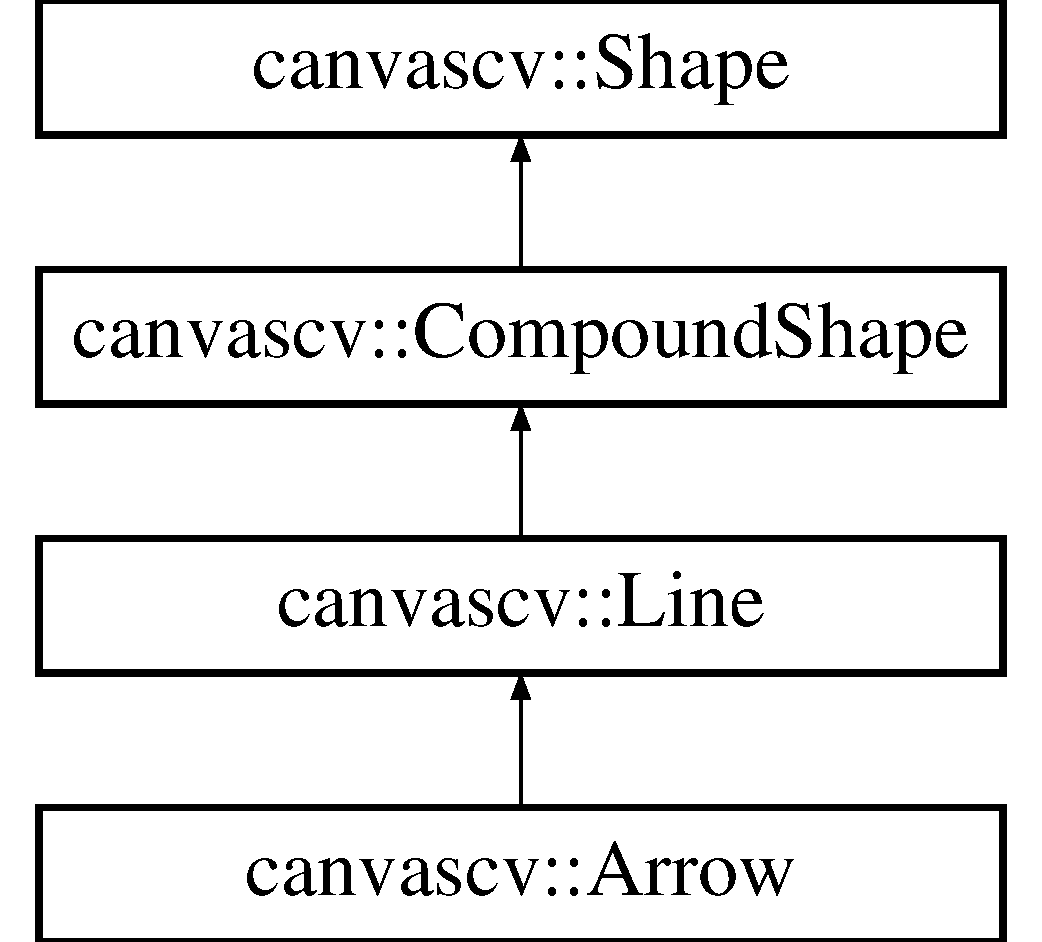
\includegraphics[height=4.000000cm]{classcanvascv_1_1Arrow}
\end{center}
\end{figure}
\subsection*{Public Member Functions}
\begin{DoxyCompactItemize}
\item 
virtual const char $\ast$ \hyperlink{classcanvascv_1_1Arrow_a4d0857dec7276f993bd390e944edef34}{get\+Type} () const 
\begin{DoxyCompactList}\small\item\em get\+Type is always implemented by derived to return the same static pointer per shape. \end{DoxyCompactList}\end{DoxyCompactItemize}
\subsection*{Protected Member Functions}
\begin{DoxyCompactItemize}
\item 
virtual void \hyperlink{classcanvascv_1_1Arrow_a8ba5b890df49a2d8fc6630df5fe80351}{draw} (cv\+::\+Mat \&canvas)
\begin{DoxyCompactList}\small\item\em draw shape on the canvas \end{DoxyCompactList}\end{DoxyCompactItemize}
\subsection*{Additional Inherited Members}


\subsection{Detailed Description}
A line in which the head has an arrow shape \begin{Desc}
\item[Examples\+: ]\par
\hyperlink{example_linecrossing_8cpp-example}{example\+\_\+linecrossing.\+cpp}.\end{Desc}


\subsection{Member Function Documentation}
\index{canvascv\+::\+Arrow@{canvascv\+::\+Arrow}!draw@{draw}}
\index{draw@{draw}!canvascv\+::\+Arrow@{canvascv\+::\+Arrow}}
\subsubsection[{\texorpdfstring{draw(cv\+::\+Mat \&canvas)}{draw(cv::Mat &canvas)}}]{\setlength{\rightskip}{0pt plus 5cm}virtual void canvascv\+::\+Arrow\+::draw (
\begin{DoxyParamCaption}
\item[{cv\+::\+Mat \&}]{canvas}
\end{DoxyParamCaption}
)\hspace{0.3cm}{\ttfamily [protected]}, {\ttfamily [virtual]}}\hypertarget{classcanvascv_1_1Arrow_a8ba5b890df49a2d8fc6630df5fe80351}{}\label{classcanvascv_1_1Arrow_a8ba5b890df49a2d8fc6630df5fe80351}

\begin{DoxyParams}{Parameters}
{\em canvas} & \\
\hline
\end{DoxyParams}


Reimplemented from \hyperlink{classcanvascv_1_1Line_aad801107019337b6e369fed331539d56}{canvascv\+::\+Line}.

\index{canvascv\+::\+Arrow@{canvascv\+::\+Arrow}!get\+Type@{get\+Type}}
\index{get\+Type@{get\+Type}!canvascv\+::\+Arrow@{canvascv\+::\+Arrow}}
\subsubsection[{\texorpdfstring{get\+Type() const }{getType() const }}]{\setlength{\rightskip}{0pt plus 5cm}virtual const char$\ast$ canvascv\+::\+Arrow\+::get\+Type (
\begin{DoxyParamCaption}
{}
\end{DoxyParamCaption}
) const\hspace{0.3cm}{\ttfamily [virtual]}}\hypertarget{classcanvascv_1_1Arrow_a4d0857dec7276f993bd390e944edef34}{}\label{classcanvascv_1_1Arrow_a4d0857dec7276f993bd390e944edef34}
\begin{DoxyReturn}{Returns}
const char $\ast$ pointer to string with shape type name 
\end{DoxyReturn}


Reimplemented from \hyperlink{classcanvascv_1_1Line_a863306159fbca892702fd3d0047b63c3}{canvascv\+::\+Line}.



The documentation for this class was generated from the following file\+:\begin{DoxyCompactItemize}
\item 
Canvas\+C\+V-\/doxygen/src/canvascv/shapes/arrow.\+h\end{DoxyCompactItemize}

\hypertarget{classcanvascv_1_1AutoLayout}{}\section{canvascv\+:\+:Auto\+Layout Class Reference}
\label{classcanvascv_1_1AutoLayout}\index{canvascv\+::\+Auto\+Layout@{canvascv\+::\+Auto\+Layout}}


The \hyperlink{classcanvascv_1_1AutoLayout}{Auto\+Layout} class.  




{\ttfamily \#include $<$autolayout.\+h$>$}

Inheritance diagram for canvascv\+:\+:Auto\+Layout\+:\begin{figure}[H]
\begin{center}
\leavevmode
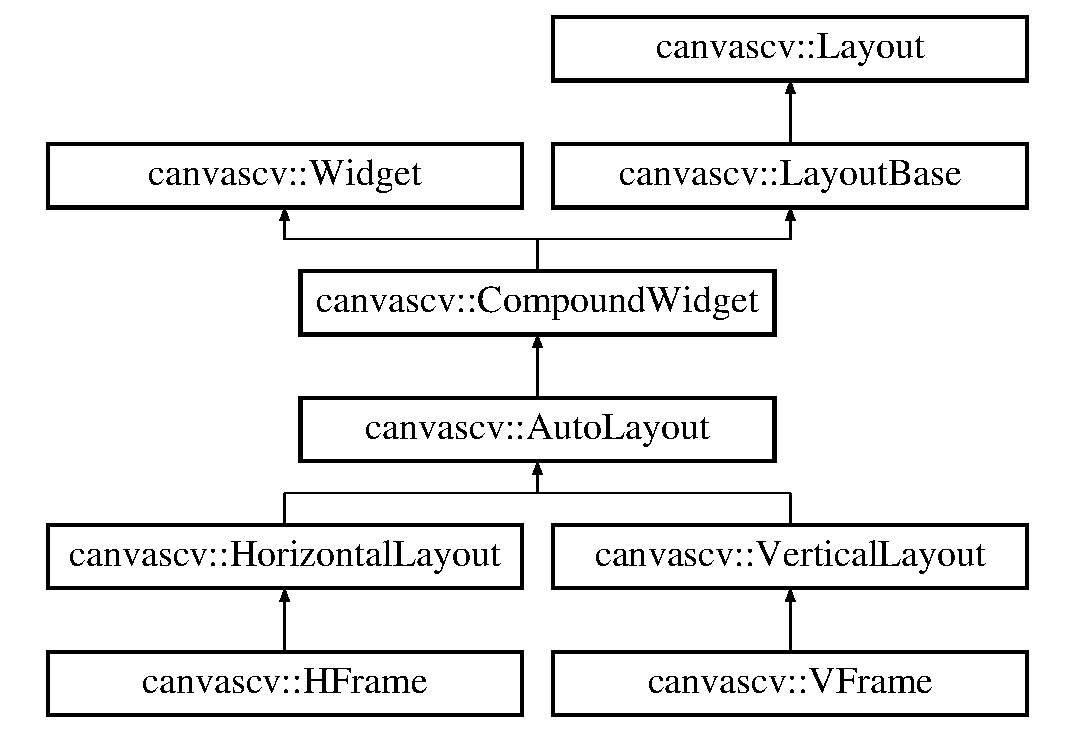
\includegraphics[height=6.000000cm]{classcanvascv_1_1AutoLayout}
\end{center}
\end{figure}
\subsection*{Public Member Functions}
\begin{DoxyCompactItemize}
\item 
int \hyperlink{classcanvascv_1_1AutoLayout_ade56b6a9186982fcf5fdcfbf39ac48df}{get\+Padding} () const 
\begin{DoxyCompactList}\small\item\em get\+Padding get number of pixels to pad from \hyperlink{classcanvascv_1_1Layout}{Layout} rect during layout \end{DoxyCompactList}\item 
void \hyperlink{classcanvascv_1_1AutoLayout_ab288ea25db0cdfe13887fdff4df1ac43}{set\+Padding} (int value)
\begin{DoxyCompactList}\small\item\em set\+Padding set number of pixels to pad from \hyperlink{classcanvascv_1_1Layout}{Layout} rect during layout \end{DoxyCompactList}\item 
virtual void \hyperlink{classcanvascv_1_1AutoLayout_a2f5bf030889e0792acc8f10d7b0ac191}{add\+Widget} (const std\+::shared\+\_\+ptr$<$ \hyperlink{classcanvascv_1_1Widget}{Widget} $>$ \&widget)\hypertarget{classcanvascv_1_1AutoLayout_a2f5bf030889e0792acc8f10d7b0ac191}{}\label{classcanvascv_1_1AutoLayout_a2f5bf030889e0792acc8f10d7b0ac191}

\begin{DoxyCompactList}\small\item\em adds the widget to this \hyperlink{classcanvascv_1_1Layout}{Layout} after removing it from it\textquotesingle{}s previous layout \end{DoxyCompactList}\item 
virtual std\+::shared\+\_\+ptr$<$ \hyperlink{classcanvascv_1_1Widget}{Widget} $>$ \hyperlink{classcanvascv_1_1AutoLayout_abc436c90f50a5331c391e351bef9e659}{rmv\+Widget} (const std\+::shared\+\_\+ptr$<$ \hyperlink{classcanvascv_1_1Widget}{Widget} $>$ \&widget)
\begin{DoxyCompactList}\small\item\em rmv\+Widget \end{DoxyCompactList}\item 
void \hyperlink{classcanvascv_1_1AutoLayout_a2e518f91b260856c3e22fcb7c61e841d}{rmv\+Widget} (int i)\hypertarget{classcanvascv_1_1AutoLayout_a2e518f91b260856c3e22fcb7c61e841d}{}\label{classcanvascv_1_1AutoLayout_a2e518f91b260856c3e22fcb7c61e841d}

\begin{DoxyCompactList}\small\item\em remove a widget at index \textquotesingle{}i\textquotesingle{} (silently ignores \textquotesingle{}i\textquotesingle{} too big) \end{DoxyCompactList}\item 
{\footnotesize template$<$typename T  = Widget$>$ }\\T $\ast$ \hyperlink{classcanvascv_1_1AutoLayout_a3735b4825af3732ebb183efdc55207f4}{at} (int index)\hypertarget{classcanvascv_1_1AutoLayout_a3735b4825af3732ebb183efdc55207f4}{}\label{classcanvascv_1_1AutoLayout_a3735b4825af3732ebb183efdc55207f4}

\begin{DoxyCompactList}\small\item\em return a widget at index \textquotesingle{}i\textquotesingle{} (or 0 if type is wrong ot \textquotesingle{}i\textquotesingle{} is too big) \end{DoxyCompactList}\item 
size\+\_\+t \hyperlink{classcanvascv_1_1AutoLayout_abda4b4eb07aab7d294b71f4135e1c8ed}{size} () const \hypertarget{classcanvascv_1_1AutoLayout_abda4b4eb07aab7d294b71f4135e1c8ed}{}\label{classcanvascv_1_1AutoLayout_abda4b4eb07aab7d294b71f4135e1c8ed}

\begin{DoxyCompactList}\small\item\em returns the number of widgets in the layout \end{DoxyCompactList}\item 
bool \hyperlink{classcanvascv_1_1AutoLayout_a33fda3ba2a72e60eec6f9cfec5bcea53}{get\+Wrap} () const \hypertarget{classcanvascv_1_1AutoLayout_a33fda3ba2a72e60eec6f9cfec5bcea53}{}\label{classcanvascv_1_1AutoLayout_a33fda3ba2a72e60eec6f9cfec5bcea53}

\begin{DoxyCompactList}\small\item\em get if the layout will wrap widgets past forced\+Width / forced\+Height \end{DoxyCompactList}\item 
void \hyperlink{classcanvascv_1_1AutoLayout_a633172f81a61be4e6840457ea538a694}{set\+Wrap} (bool value)\hypertarget{classcanvascv_1_1AutoLayout_a633172f81a61be4e6840457ea538a694}{}\label{classcanvascv_1_1AutoLayout_a633172f81a61be4e6840457ea538a694}

\begin{DoxyCompactList}\small\item\em set if the layout will wrap widgets past forced\+Width / forced\+Height \end{DoxyCompactList}\item 
int \hyperlink{classcanvascv_1_1AutoLayout_adc7737dce041188285c0026efb3d7c08}{get\+Max\+Widget\+Width} ()\hypertarget{classcanvascv_1_1AutoLayout_adc7737dce041188285c0026efb3d7c08}{}\label{classcanvascv_1_1AutoLayout_adc7737dce041188285c0026efb3d7c08}

\begin{DoxyCompactList}\small\item\em get the maximum width from all contained widgets \end{DoxyCompactList}\item 
int \hyperlink{classcanvascv_1_1AutoLayout_a7b2458bbef0c160ab0e2b138c802d188}{get\+Max\+Widget\+Height} ()\hypertarget{classcanvascv_1_1AutoLayout_a7b2458bbef0c160ab0e2b138c802d188}{}\label{classcanvascv_1_1AutoLayout_a7b2458bbef0c160ab0e2b138c802d188}

\begin{DoxyCompactList}\small\item\em get the maximum height from all contained widgets \end{DoxyCompactList}\end{DoxyCompactItemize}
\subsection*{Additional Inherited Members}


\subsection{Detailed Description}
Base class for all \hyperlink{classcanvascv_1_1Layout}{Layout} managers which are also widgets (not the \hyperlink{classcanvascv_1_1Canvas}{Canvas} class) 

\subsection{Member Function Documentation}
\index{canvascv\+::\+Auto\+Layout@{canvascv\+::\+Auto\+Layout}!get\+Padding@{get\+Padding}}
\index{get\+Padding@{get\+Padding}!canvascv\+::\+Auto\+Layout@{canvascv\+::\+Auto\+Layout}}
\subsubsection[{\texorpdfstring{get\+Padding() const }{getPadding() const }}]{\setlength{\rightskip}{0pt plus 5cm}int canvascv\+::\+Auto\+Layout\+::get\+Padding (
\begin{DoxyParamCaption}
{}
\end{DoxyParamCaption}
) const}\hypertarget{classcanvascv_1_1AutoLayout_ade56b6a9186982fcf5fdcfbf39ac48df}{}\label{classcanvascv_1_1AutoLayout_ade56b6a9186982fcf5fdcfbf39ac48df}
\begin{DoxyVerb}   +----------------------+
   |       PADDING        |
   |   +--------------+   |
   | P |   Widget     | P |
   | A +--------------+ A |
   | D     SPACING      D |
   | D +--------------+ D |
   | I |   Widget     | I |
   | N +--------------+ N |
   | G     PADDING      G |
   +----------------------+
\end{DoxyVerb}
 \begin{DoxyReturn}{Returns}
padding in pixels 
\end{DoxyReturn}
\index{canvascv\+::\+Auto\+Layout@{canvascv\+::\+Auto\+Layout}!rmv\+Widget@{rmv\+Widget}}
\index{rmv\+Widget@{rmv\+Widget}!canvascv\+::\+Auto\+Layout@{canvascv\+::\+Auto\+Layout}}
\subsubsection[{\texorpdfstring{rmv\+Widget(const std\+::shared\+\_\+ptr$<$ Widget $>$ \&widget)}{rmvWidget(const std::shared_ptr< Widget > &widget)}}]{\setlength{\rightskip}{0pt plus 5cm}virtual std\+::shared\+\_\+ptr$<${\bf Widget}$>$ canvascv\+::\+Auto\+Layout\+::rmv\+Widget (
\begin{DoxyParamCaption}
\item[{const std\+::shared\+\_\+ptr$<$ {\bf Widget} $>$ \&}]{widget}
\end{DoxyParamCaption}
)\hspace{0.3cm}{\ttfamily [virtual]}}\hypertarget{classcanvascv_1_1AutoLayout_abc436c90f50a5331c391e351bef9e659}{}\label{classcanvascv_1_1AutoLayout_abc436c90f50a5331c391e351bef9e659}

\begin{DoxyParams}{Parameters}
{\em widget} & will be removed from this \hyperlink{classcanvascv_1_1Layout}{Layout} \\
\hline
\end{DoxyParams}
\begin{DoxyReturn}{Returns}
filled shared\+\_\+ptr to removed widget or empty if not found 
\end{DoxyReturn}
\begin{DoxyNote}{Note}
Widgets must be in layouts to be displayed correctly. 
\end{DoxyNote}


Reimplemented from \hyperlink{classcanvascv_1_1CompoundWidget_ad4a37bf31f9cf6410b41526a5b83c75a}{canvascv\+::\+Compound\+Widget}.

\index{canvascv\+::\+Auto\+Layout@{canvascv\+::\+Auto\+Layout}!set\+Padding@{set\+Padding}}
\index{set\+Padding@{set\+Padding}!canvascv\+::\+Auto\+Layout@{canvascv\+::\+Auto\+Layout}}
\subsubsection[{\texorpdfstring{set\+Padding(int value)}{setPadding(int value)}}]{\setlength{\rightskip}{0pt plus 5cm}void canvascv\+::\+Auto\+Layout\+::set\+Padding (
\begin{DoxyParamCaption}
\item[{int}]{value}
\end{DoxyParamCaption}
)}\hypertarget{classcanvascv_1_1AutoLayout_ab288ea25db0cdfe13887fdff4df1ac43}{}\label{classcanvascv_1_1AutoLayout_ab288ea25db0cdfe13887fdff4df1ac43}
\begin{DoxyVerb}   +----------------------+
   |       PADDING        |
   |   +--------------+   |
   | P |   Widget     | P |
   | A +--------------+ A |
   | D     SPACING      D |
   | D +--------------+ D |
   | I |   Widget     | I |
   | N +--------------+ N |
   | G     PADDING      G |
   +----------------------+
\end{DoxyVerb}
 

The documentation for this class was generated from the following file\+:\begin{DoxyCompactItemize}
\item 
Canvas\+C\+V-\/doxygen/src/canvascv/widgets/autolayout.\+h\end{DoxyCompactItemize}

\hypertarget{classcanvascv_1_1Button}{}\section{canvascv\+:\+:Button Class Reference}
\label{classcanvascv_1_1Button}\index{canvascv\+::\+Button@{canvascv\+::\+Button}}


The \hyperlink{classcanvascv_1_1Button}{Button} class.  




{\ttfamily \#include $<$button.\+h$>$}

Inheritance diagram for canvascv\+:\+:Button\+:\begin{figure}[H]
\begin{center}
\leavevmode
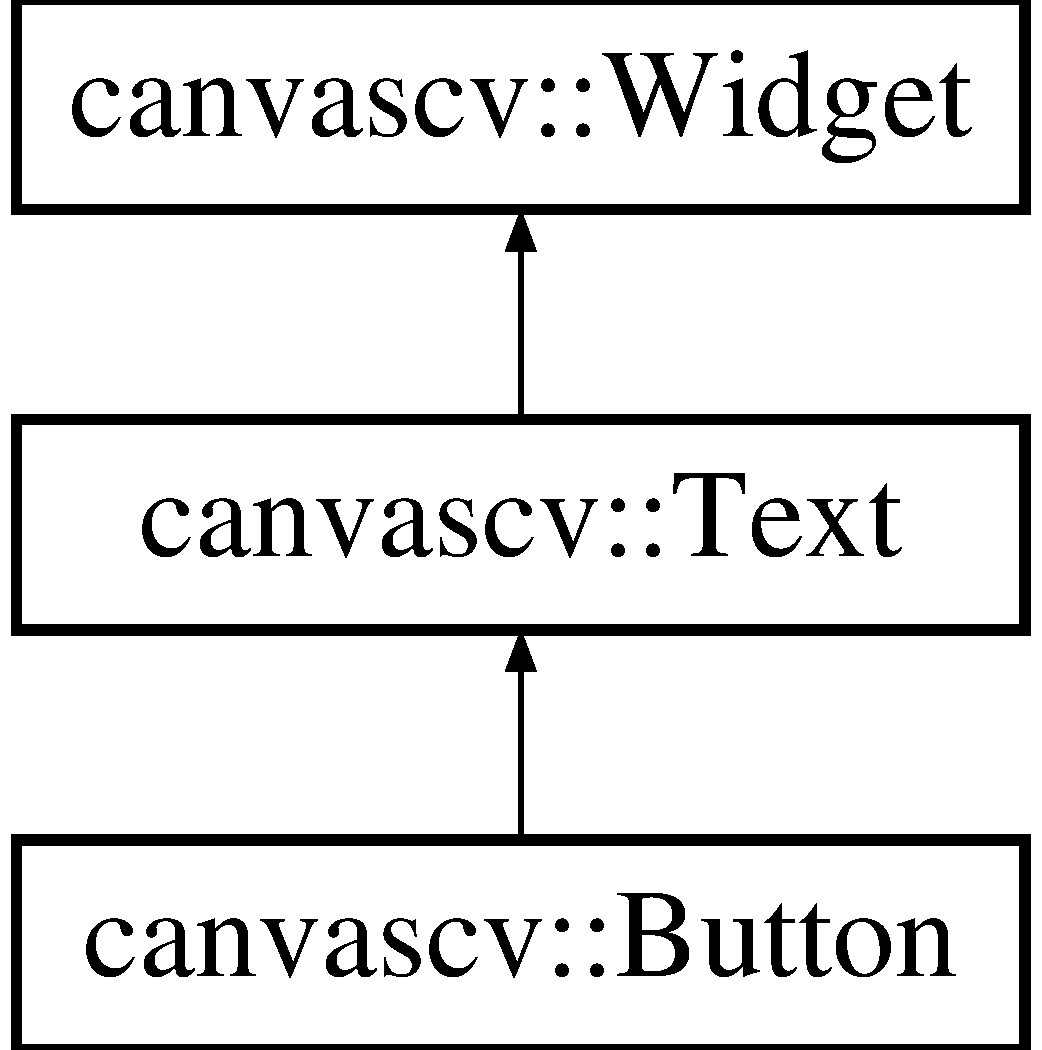
\includegraphics[height=3.000000cm]{classcanvascv_1_1Button}
\end{center}
\end{figure}
\subsection*{Public Member Functions}
\begin{DoxyCompactItemize}
\item 
void \hyperlink{classcanvascv_1_1Button_a7d2c79daa9d22bf02c2cc978ff10df7e}{set\+Flat\+Button} ()\hypertarget{classcanvascv_1_1Button_a7d2c79daa9d22bf02c2cc978ff10df7e}{}\label{classcanvascv_1_1Button_a7d2c79daa9d22bf02c2cc978ff10df7e}

\begin{DoxyCompactList}\small\item\em The button will always have a F\+L\+AT relief. \end{DoxyCompactList}\item 
void \hyperlink{classcanvascv_1_1Button_a274f428bce039ba2159b78d790c3ed94}{on\+Press} (\hyperlink{classcanvascv_1_1Widget_ad27bca771ee1c14454c77c91d9d49925}{C\+B\+Widget} value)\hypertarget{classcanvascv_1_1Button_a274f428bce039ba2159b78d790c3ed94}{}\label{classcanvascv_1_1Button_a274f428bce039ba2159b78d790c3ed94}

\begin{DoxyCompactList}\small\item\em Call a user CB when pressed. \end{DoxyCompactList}\item 
virtual const char $\ast$ \hyperlink{classcanvascv_1_1Button_ace294c72ce39507268ffd752f4ca0034}{get\+Type} () const 
\begin{DoxyCompactList}\small\item\em get\+Type is always implemented by derived to return the same static pointer per widget. \end{DoxyCompactList}\end{DoxyCompactItemize}
\subsection*{Static Public Member Functions}
\begin{DoxyCompactItemize}
\item 
static std\+::shared\+\_\+ptr$<$ \hyperlink{classcanvascv_1_1Button}{Button} $>$ \hyperlink{classcanvascv_1_1Button_a3557ea02dfca8d6cb92181a2d2b88112}{create} (\hyperlink{classcanvascv_1_1Layout}{Layout} \&layout, const cv\+::\+Point \&pos, const std\+::string \&button\+Text, const std\+::string \&status\+Msg=\char`\"{}\char`\"{}, \hyperlink{classcanvascv_1_1Widget_ad27bca771ee1c14454c77c91d9d49925}{C\+B\+Widget} cb\+Val=\hyperlink{classcanvascv_1_1Widget_ad27bca771ee1c14454c77c91d9d49925}{C\+B\+Widget}())
\begin{DoxyCompactList}\small\item\em create a button widget \end{DoxyCompactList}\item 
static std\+::shared\+\_\+ptr$<$ \hyperlink{classcanvascv_1_1Button}{Button} $>$ \hyperlink{classcanvascv_1_1Button_afcef2e139661b2b07da904899d83cfc8}{create} (\hyperlink{classcanvascv_1_1Layout}{Layout} \&layout, const std\+::string \&button\+Text, const std\+::string \&status\+Msg=\char`\"{}\char`\"{}, \hyperlink{classcanvascv_1_1Widget_ad27bca771ee1c14454c77c91d9d49925}{C\+B\+Widget} cb\+Val=\hyperlink{classcanvascv_1_1Widget_ad27bca771ee1c14454c77c91d9d49925}{C\+B\+Widget}())\hypertarget{classcanvascv_1_1Button_afcef2e139661b2b07da904899d83cfc8}{}\label{classcanvascv_1_1Button_afcef2e139661b2b07da904899d83cfc8}

\begin{DoxyCompactList}\small\item\em a convinient version to the above without the \textquotesingle{}pos\textquotesingle{} argument \end{DoxyCompactList}\end{DoxyCompactItemize}
\subsection*{Additional Inherited Members}


\subsection{Detailed Description}
a button widget to use on the Open\+CV Window \begin{Desc}
\item[Examples\+: ]\par
\hyperlink{example_add_widget_8cpp-example}{example\+\_\+add\+\_\+widget.\+cpp}.\end{Desc}


\subsection{Member Function Documentation}
\index{canvascv\+::\+Button@{canvascv\+::\+Button}!create@{create}}
\index{create@{create}!canvascv\+::\+Button@{canvascv\+::\+Button}}
\subsubsection[{\texorpdfstring{create(\+Layout \&layout, const cv\+::\+Point \&pos, const std\+::string \&button\+Text, const std\+::string \&status\+Msg="""", C\+B\+Widget cb\+Val=\+C\+B\+Widget())}{create(Layout &layout, const cv::Point &pos, const std::string &buttonText, const std::string &statusMsg="", CBWidget cbVal=CBWidget())}}]{\setlength{\rightskip}{0pt plus 5cm}static std\+::shared\+\_\+ptr$<${\bf Button}$>$ canvascv\+::\+Button\+::create (
\begin{DoxyParamCaption}
\item[{{\bf Layout} \&}]{layout, }
\item[{const cv\+::\+Point \&}]{pos, }
\item[{const std\+::string \&}]{button\+Text, }
\item[{const std\+::string \&}]{status\+Msg = {\ttfamily \char`\"{}\char`\"{}}, }
\item[{{\bf C\+B\+Widget}}]{cb\+Val = {\ttfamily {\bf C\+B\+Widget}()}}
\end{DoxyParamCaption}
)\hspace{0.3cm}{\ttfamily [static]}}\hypertarget{classcanvascv_1_1Button_a3557ea02dfca8d6cb92181a2d2b88112}{}\label{classcanvascv_1_1Button_a3557ea02dfca8d6cb92181a2d2b88112}

\begin{DoxyParams}{Parameters}
{\em layout} & widgets are placed in layouts Canvas/\+V\+Frame/\+H\+Frame/... \\
\hline
{\em pos} & location in the \hyperlink{classcanvascv_1_1Layout}{Layout} (Layouts can ignore that) \\
\hline
{\em button\+Text} & what to write on the button \\
\hline
{\em status\+Msg} & what to write during hover over the button \\
\hline
{\em cb\+Val} & a callback to invoke when the button is pressed \\
\hline
\end{DoxyParams}
\begin{DoxyReturn}{Returns}
a smart pointer copy of the object kept in the \hyperlink{classcanvascv_1_1Layout}{Layout} 
\end{DoxyReturn}
\begin{Desc}
\item[Examples\+: ]\par
\hyperlink{example_add_widget_8cpp-example}{example\+\_\+add\+\_\+widget.\+cpp}, and \hyperlink{example_shapes_widgets_8cpp-example}{example\+\_\+shapes\+\_\+widgets.\+cpp}.\end{Desc}
\index{canvascv\+::\+Button@{canvascv\+::\+Button}!get\+Type@{get\+Type}}
\index{get\+Type@{get\+Type}!canvascv\+::\+Button@{canvascv\+::\+Button}}
\subsubsection[{\texorpdfstring{get\+Type() const }{getType() const }}]{\setlength{\rightskip}{0pt plus 5cm}virtual const char$\ast$ canvascv\+::\+Button\+::get\+Type (
\begin{DoxyParamCaption}
{}
\end{DoxyParamCaption}
) const\hspace{0.3cm}{\ttfamily [virtual]}}\hypertarget{classcanvascv_1_1Button_ace294c72ce39507268ffd752f4ca0034}{}\label{classcanvascv_1_1Button_ace294c72ce39507268ffd752f4ca0034}
\begin{DoxyReturn}{Returns}
const char $\ast$ pointer to string with widget type name 
\end{DoxyReturn}


Reimplemented from \hyperlink{classcanvascv_1_1Text_ae81d87d43167c2e8d1e58fa620a80579}{canvascv\+::\+Text}.



The documentation for this class was generated from the following file\+:\begin{DoxyCompactItemize}
\item 
Canvas\+C\+V-\/doxygen/src/canvascv/widgets/button.\+h\end{DoxyCompactItemize}

\hypertarget{classcanvascv_1_1Canvas}{}\section{canvascv\+:\+:Canvas Class Reference}
\label{classcanvascv_1_1Canvas}\index{canvascv\+::\+Canvas@{canvascv\+::\+Canvas}}


The \hyperlink{classcanvascv_1_1Canvas}{Canvas} class is the entry point into Canvas\+CV.  




{\ttfamily \#include $<$canvas.\+h$>$}

Inheritance diagram for canvascv\+:\+:Canvas\+:\begin{figure}[H]
\begin{center}
\leavevmode
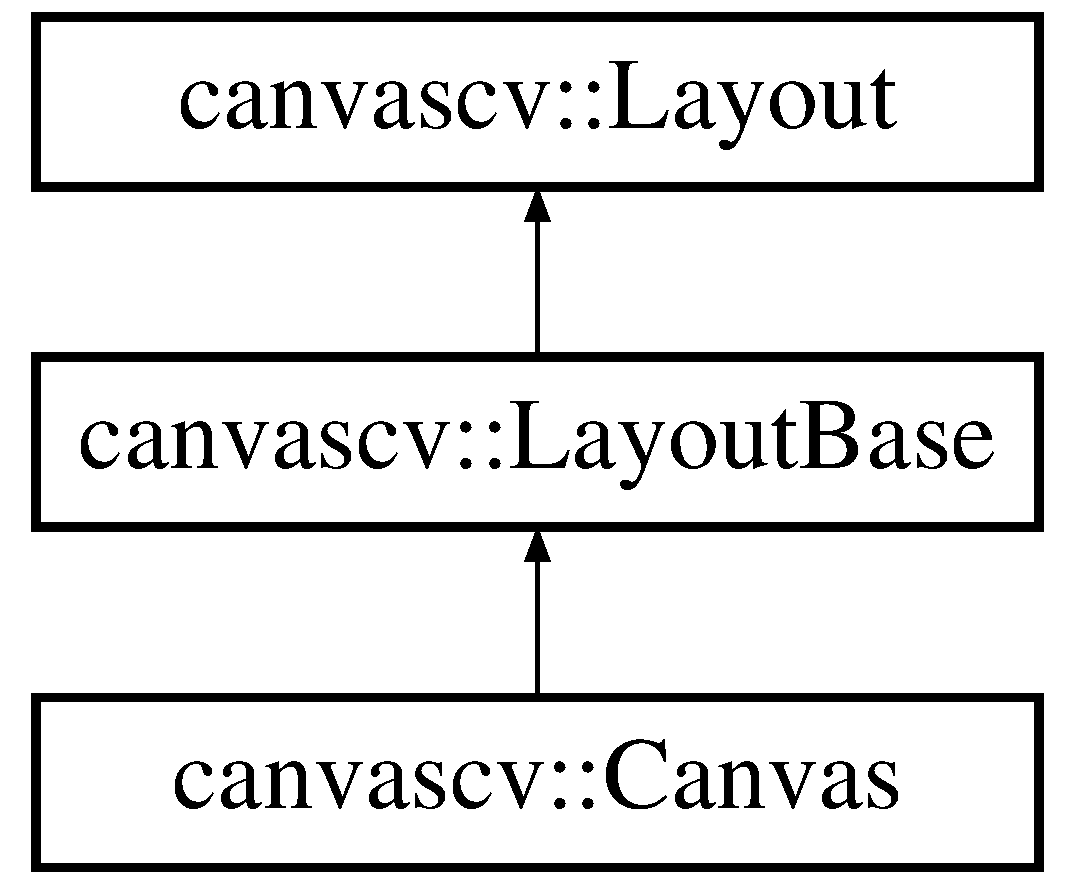
\includegraphics[height=3.000000cm]{classcanvascv_1_1Canvas}
\end{center}
\end{figure}
\subsection*{Public Types}
\begin{DoxyCompactItemize}
\item 
typedef std\+::function$<$ void(\hyperlink{classcanvascv_1_1Shape}{Shape} $\ast$)$>$ \hyperlink{classcanvascv_1_1Canvas_a6436ebb5dbadc3dbf9de3da8a499cf44}{C\+B\+Canvas\+Shape}\hypertarget{classcanvascv_1_1Canvas_a6436ebb5dbadc3dbf9de3da8a499cf44}{}\label{classcanvascv_1_1Canvas_a6436ebb5dbadc3dbf9de3da8a499cf44}

\begin{DoxyCompactList}\small\item\em notification on shapes create/modify/delete from this \hyperlink{classcanvascv_1_1Canvas}{Canvas} instance \end{DoxyCompactList}\end{DoxyCompactItemize}
\subsection*{Public Member Functions}
\begin{DoxyCompactItemize}
\item 
\hyperlink{classcanvascv_1_1Canvas_a7049e8c687a2ac33331820d32f4f6464}{Canvas} (const std\+::string \&win\+Name\+Val, cv\+::\+Size size\+Val=cv\+::\+Size())
\begin{DoxyCompactList}\small\item\em \hyperlink{classcanvascv_1_1Canvas}{Canvas}. \end{DoxyCompactList}\item 
\hyperlink{classcanvascv_1_1Canvas_a178be13c77efe0d5768fb7ca09873711}{$\sim$\+Canvas} ()\hypertarget{classcanvascv_1_1Canvas_a178be13c77efe0d5768fb7ca09873711}{}\label{classcanvascv_1_1Canvas_a178be13c77efe0d5768fb7ca09873711}

\begin{DoxyCompactList}\small\item\em release all shapes and widgets. \hyperlink{classcanvascv_1_1Shape}{Shape} callbacks are invoked doe delete. \end{DoxyCompactList}\item 
void \hyperlink{classcanvascv_1_1Canvas_a018c66e277de7904b8146ea3f3feebdd}{redraw\+On} (const cv\+::\+Mat \&src, cv\+::\+Mat \&dst)
\begin{DoxyCompactList}\small\item\em redraw\+On draws the shapes on dst \end{DoxyCompactList}\item 
void \hyperlink{classcanvascv_1_1Canvas_a0eed02e6923d903c3af1bf6692ad87fe}{redraw\+On} (cv\+::\+Mat \&dst)
\begin{DoxyCompactList}\small\item\em redraw\+On \end{DoxyCompactList}\item 
void \hyperlink{classcanvascv_1_1Canvas_a441c5882c7ebebd454a306b3c3478ae7}{set\+Image} (const cv\+::\+Mat \&img)
\begin{DoxyCompactList}\small\item\em set\+Image \end{DoxyCompactList}\item 
bool \hyperlink{classcanvascv_1_1Canvas_abe53228080133efe5d9fecf6982b823e}{on\+Mouse\+Press} (const cv\+::\+Point \&pos)\hypertarget{classcanvascv_1_1Canvas_abe53228080133efe5d9fecf6982b823e}{}\label{classcanvascv_1_1Canvas_abe53228080133efe5d9fecf6982b823e}

\begin{DoxyCompactList}\small\item\em You should delegate Open\+CV mouse callback events to this method -\/ returns true if did something at pos. \end{DoxyCompactList}\item 
void \hyperlink{classcanvascv_1_1Canvas_aca936fe492da286d5fb8eabbcd061793}{on\+Mouse\+Release} (const cv\+::\+Point \&pos)\hypertarget{classcanvascv_1_1Canvas_aca936fe492da286d5fb8eabbcd061793}{}\label{classcanvascv_1_1Canvas_aca936fe492da286d5fb8eabbcd061793}

\begin{DoxyCompactList}\small\item\em You should delegate Open\+CV mouse callback events to this method. \end{DoxyCompactList}\item 
void \hyperlink{classcanvascv_1_1Canvas_a1189823898c4022fd0eed4cfb99535c2}{on\+Mouse\+Move} (const cv\+::\+Point \&pos)\hypertarget{classcanvascv_1_1Canvas_a1189823898c4022fd0eed4cfb99535c2}{}\label{classcanvascv_1_1Canvas_a1189823898c4022fd0eed4cfb99535c2}

\begin{DoxyCompactList}\small\item\em You should delegate Open\+CV mouse callback events to this method. \end{DoxyCompactList}\item 
std\+::shared\+\_\+ptr$<$ \hyperlink{classcanvascv_1_1Shape}{Shape} $>$ \hyperlink{classcanvascv_1_1Canvas_a630ac92458f1718d0c597e96dd5a4aef}{create\+Shape} (std\+::string type, const cv\+::\+Point \&pos=cv\+::\+Point(0, 0))
\begin{DoxyCompactList}\small\item\em create\+Shape \end{DoxyCompactList}\item 
{\footnotesize template$<$class T $>$ }\\std\+::shared\+\_\+ptr$<$ T $>$ \hyperlink{classcanvascv_1_1Canvas_ac126ef1547509744d9968ba83ddfef36}{create\+Shape} (const cv\+::\+Point \&pos=cv\+::\+Point(0, 0))
\begin{DoxyCompactList}\small\item\em create\+Shape \end{DoxyCompactList}\item 
std\+::string \hyperlink{classcanvascv_1_1Canvas_a910107e17ee39da2074f9688e2a307ae}{get\+Shape\+Type} () const 
\begin{DoxyCompactList}\small\item\em get default shape type to draw \end{DoxyCompactList}\item 
void \hyperlink{classcanvascv_1_1Canvas_ac61735c6f4cb6a88d84331540ab25d39}{set\+Shape\+Type} (std\+::string value)
\begin{DoxyCompactList}\small\item\em set default shape type to draw (could be \char`\"{}\char`\"{}) \end{DoxyCompactList}\item 
void \hyperlink{classcanvascv_1_1Canvas_a2fb88addb88a21757d4272e64acd30ae}{delete\+Active} ()\hypertarget{classcanvascv_1_1Canvas_a2fb88addb88a21757d4272e64acd30ae}{}\label{classcanvascv_1_1Canvas_a2fb88addb88a21757d4272e64acd30ae}

\begin{DoxyCompactList}\small\item\em delete shape currenty selected \end{DoxyCompactList}\item 
void \hyperlink{classcanvascv_1_1Canvas_a4cabdb76b4f6854e957a065c29ab5669}{delete\+Shape} (const std\+::shared\+\_\+ptr$<$ \hyperlink{classcanvascv_1_1Shape}{Shape} $>$ \&shape)\hypertarget{classcanvascv_1_1Canvas_a4cabdb76b4f6854e957a065c29ab5669}{}\label{classcanvascv_1_1Canvas_a4cabdb76b4f6854e957a065c29ab5669}

\begin{DoxyCompactList}\small\item\em delete specific shape \end{DoxyCompactList}\item 
void \hyperlink{classcanvascv_1_1Canvas_ab72c0ea97fe435d9ce2aeffb4116faed}{delete\+Widget} (const std\+::shared\+\_\+ptr$<$ \hyperlink{classcanvascv_1_1Widget}{Widget} $>$ \&widget)\hypertarget{classcanvascv_1_1Canvas_ab72c0ea97fe435d9ce2aeffb4116faed}{}\label{classcanvascv_1_1Canvas_ab72c0ea97fe435d9ce2aeffb4116faed}

\begin{DoxyCompactList}\small\item\em delete specific widget \end{DoxyCompactList}\item 
void \hyperlink{classcanvascv_1_1Canvas_a64a459b16965e23de992cd2a301c68f4}{notify\+On\+Shape\+Create} (\hyperlink{classcanvascv_1_1Canvas_a6436ebb5dbadc3dbf9de3da8a499cf44}{C\+B\+Canvas\+Shape} cb)
\begin{DoxyCompactList}\small\item\em used to register for notifications on shape creation \end{DoxyCompactList}\item 
void \hyperlink{classcanvascv_1_1Canvas_a5a6da8ae08b08a20d7fe15564bda5515}{notify\+On\+Shape\+Modify} (\hyperlink{classcanvascv_1_1Canvas_a6436ebb5dbadc3dbf9de3da8a499cf44}{C\+B\+Canvas\+Shape} cb)
\begin{DoxyCompactList}\small\item\em used to register for notifications on shape modification (actually when it is deselected) \end{DoxyCompactList}\item 
void \hyperlink{classcanvascv_1_1Canvas_a1e7c26b39fd247e85941a6542f1b94c3}{notify\+On\+Shape\+Delete} (\hyperlink{classcanvascv_1_1Canvas_a6436ebb5dbadc3dbf9de3da8a499cf44}{C\+B\+Canvas\+Shape} cb)
\begin{DoxyCompactList}\small\item\em used to register for notifications on shape deletion \end{DoxyCompactList}\item 
void \hyperlink{classcanvascv_1_1Canvas_a8aa6686036b8a1a006718ae62f44b6c2}{clear\+Shapes} ()\hypertarget{classcanvascv_1_1Canvas_a8aa6686036b8a1a006718ae62f44b6c2}{}\label{classcanvascv_1_1Canvas_a8aa6686036b8a1a006718ae62f44b6c2}

\begin{DoxyCompactList}\small\item\em clear all shapes from \hyperlink{classcanvascv_1_1Canvas}{Canvas} \end{DoxyCompactList}\item 
void \hyperlink{classcanvascv_1_1Canvas_a94ee58b125af1d49baf921b7a65d0d8d}{clear\+Widgets} ()\hypertarget{classcanvascv_1_1Canvas_a94ee58b125af1d49baf921b7a65d0d8d}{}\label{classcanvascv_1_1Canvas_a94ee58b125af1d49baf921b7a65d0d8d}

\begin{DoxyCompactList}\small\item\em clear all widgets from \hyperlink{classcanvascv_1_1Canvas}{Canvas} \end{DoxyCompactList}\item 
{\footnotesize template$<$class T $>$ }\\void \hyperlink{classcanvascv_1_1Canvas_a6201675a6b8a13b3e004456225987dfa}{get\+Shapes} (std\+::list$<$ std\+::shared\+\_\+ptr$<$ T $>$$>$ \&result)
\begin{DoxyCompactList}\small\item\em get\+Shapes of a specific type \end{DoxyCompactList}\item 
std\+::shared\+\_\+ptr$<$ \hyperlink{classcanvascv_1_1Shape}{Shape} $>$ \hyperlink{classcanvascv_1_1Canvas_a7b799712dccb4316648a3c1a09a8279f}{get\+Shape} (int id)
\begin{DoxyCompactList}\small\item\em get\+Shape \end{DoxyCompactList}\item 
void \hyperlink{classcanvascv_1_1Canvas_aec742570f7a4fd9dc2671826ca3a159a}{get\+Shapes} (const cv\+::\+Point \&pos, std\+::list$<$ std\+::shared\+\_\+ptr$<$ \hyperlink{classcanvascv_1_1Shape}{Shape} $>$$>$ \&result)
\begin{DoxyCompactList}\small\item\em get\+Shapes \end{DoxyCompactList}\item 
void \hyperlink{classcanvascv_1_1Canvas_afbc5ba3255edc06c63ce2a64e732754b}{disable\+Screen\+Text} ()\hypertarget{classcanvascv_1_1Canvas_afbc5ba3255edc06c63ce2a64e732754b}{}\label{classcanvascv_1_1Canvas_afbc5ba3255edc06c63ce2a64e732754b}

\begin{DoxyCompactList}\small\item\em disable the top left text area for manual user messages \end{DoxyCompactList}\item 
void \hyperlink{classcanvascv_1_1Canvas_ad307658a70d97c360af99d3738fee972}{disable\+Status\+Msg} ()\hypertarget{classcanvascv_1_1Canvas_ad307658a70d97c360af99d3738fee972}{}\label{classcanvascv_1_1Canvas_ad307658a70d97c360af99d3738fee972}

\begin{DoxyCompactList}\small\item\em disable the bottom left text area for auto status messages \end{DoxyCompactList}\item 
void \hyperlink{classcanvascv_1_1Canvas_ae68d3277e738d349232400b38f0e5f9e}{enable\+Screen\+Text} (cv\+::\+Scalar color=\hyperlink{classcanvascv_1_1Colors_a934f65d826ab8b22e5bcfa6ce7816dbe}{Colors\+::\+Black}, cv\+::\+Scalar bg\+Color=\hyperlink{classcanvascv_1_1Colors_a4c2258611a1932339c02df35504f8f6d}{Colors\+::\+Light\+Gray}, double scale=Consts\+::\+D\+E\+F\+A\+U\+L\+T\+\_\+\+F\+O\+N\+T\+\_\+\+S\+C\+A\+LE, int thickness=Consts\+::\+D\+E\+F\+A\+U\+L\+T\+\_\+\+F\+O\+N\+T\+\_\+\+T\+H\+I\+C\+K\+N\+E\+SS, uchar alpha=80, int font\+Face=Consts\+::\+D\+E\+F\+A\+U\+L\+T\+\_\+\+F\+O\+NT)
\begin{DoxyCompactList}\small\item\em enable\+Screen\+Text enables the top left text area for manual user messages \end{DoxyCompactList}\item 
void \hyperlink{classcanvascv_1_1Canvas_a402c43a42c0089c48a96e5303c1c1fe8}{enable\+Status\+Msg} (cv\+::\+Scalar color=\hyperlink{classcanvascv_1_1Colors_a463fb59b35fb56e7a4eaa5976baaa411}{Colors\+::\+Orange}, cv\+::\+Scalar bg\+Color=\hyperlink{classcanvascv_1_1Colors_a4c2258611a1932339c02df35504f8f6d}{Colors\+::\+Light\+Gray}, double scale=Consts\+::\+D\+E\+F\+A\+U\+L\+T\+\_\+\+F\+O\+N\+T\+\_\+\+S\+C\+A\+LE, int thickness=Consts\+::\+D\+E\+F\+A\+U\+L\+T\+\_\+\+F\+O\+N\+T\+\_\+\+T\+H\+I\+C\+K\+N\+E\+SS, uchar alpha=80, int font\+Face=Consts\+::\+D\+E\+F\+A\+U\+L\+T\+\_\+\+F\+O\+NT)
\begin{DoxyCompactList}\small\item\em enable\+Status\+Msg enables the bottom left text area for auto status messages \end{DoxyCompactList}\item 
void \hyperlink{classcanvascv_1_1Canvas_a14828809edd29d789170284a86f16f23}{set\+Default\+Status\+Msg} (const std\+::string \&msg)\hypertarget{classcanvascv_1_1Canvas_a14828809edd29d789170284a86f16f23}{}\label{classcanvascv_1_1Canvas_a14828809edd29d789170284a86f16f23}

\begin{DoxyCompactList}\small\item\em set the default status message (active widget and shapes will override it) \end{DoxyCompactList}\item 
std\+::string \hyperlink{classcanvascv_1_1Canvas_a020df071c9ef8dd6a0582accb75553df}{get\+Default\+Status\+Msg} () const \hypertarget{classcanvascv_1_1Canvas_a020df071c9ef8dd6a0582accb75553df}{}\label{classcanvascv_1_1Canvas_a020df071c9ef8dd6a0582accb75553df}

\begin{DoxyCompactList}\small\item\em get the default status message (active widget and shapes will override it) \end{DoxyCompactList}\item 
void \hyperlink{classcanvascv_1_1Canvas_aaedea276b82a8a4cfc0895ae81113cfd}{set\+Screen\+Text} (const std\+::string \&msg)\hypertarget{classcanvascv_1_1Canvas_aaedea276b82a8a4cfc0895ae81113cfd}{}\label{classcanvascv_1_1Canvas_aaedea276b82a8a4cfc0895ae81113cfd}

\begin{DoxyCompactList}\small\item\em manually set the screen text message. It remains until disabled or changed. \end{DoxyCompactList}\item 
void \hyperlink{classcanvascv_1_1Canvas_ab9ffc28f7a21e1375da18cc4f03343ae}{set\+Size} (const cv\+::\+Size \&value)\hypertarget{classcanvascv_1_1Canvas_ab9ffc28f7a21e1375da18cc4f03343ae}{}\label{classcanvascv_1_1Canvas_ab9ffc28f7a21e1375da18cc4f03343ae}

\begin{DoxyCompactList}\small\item\em set the \hyperlink{classcanvascv_1_1Canvas}{Canvas} size to match the cv\+::\+Mat we\textquotesingle{}ll use in redraw\+On; \end{DoxyCompactList}\item 
cv\+::\+Size \hyperlink{classcanvascv_1_1Canvas_a749efce55cfc1a16f6fdb91fab435bc4}{get\+Size} ()\hypertarget{classcanvascv_1_1Canvas_a749efce55cfc1a16f6fdb91fab435bc4}{}\label{classcanvascv_1_1Canvas_a749efce55cfc1a16f6fdb91fab435bc4}

\begin{DoxyCompactList}\small\item\em get the \hyperlink{classcanvascv_1_1Canvas}{Canvas} size \end{DoxyCompactList}\item 
virtual void \hyperlink{classcanvascv_1_1Canvas_a830b59fb09fe8f493c895d96316f6f36}{add\+Widget} (const std\+::shared\+\_\+ptr$<$ \hyperlink{classcanvascv_1_1Widget}{Widget} $>$ \&widget)\hypertarget{classcanvascv_1_1Canvas_a830b59fb09fe8f493c895d96316f6f36}{}\label{classcanvascv_1_1Canvas_a830b59fb09fe8f493c895d96316f6f36}

\begin{DoxyCompactList}\small\item\em adds the widget to this \hyperlink{classcanvascv_1_1Layout}{Layout} after removing it from it\textquotesingle{}s previous layout \end{DoxyCompactList}\item 
virtual std\+::shared\+\_\+ptr$<$ \hyperlink{classcanvascv_1_1Widget}{Widget} $>$ \hyperlink{classcanvascv_1_1Canvas_a70248a9be2eedcacad74c9be5fd615eb}{rmv\+Widget} (const std\+::shared\+\_\+ptr$<$ \hyperlink{classcanvascv_1_1Widget}{Widget} $>$ \&widget)
\begin{DoxyCompactList}\small\item\em rmv\+Widget \end{DoxyCompactList}\item 
bool \hyperlink{classcanvascv_1_1Canvas_afe6a2955a5bbee8903350b4fba3f4473}{get\+On} () const \hypertarget{classcanvascv_1_1Canvas_afe6a2955a5bbee8903350b4fba3f4473}{}\label{classcanvascv_1_1Canvas_afe6a2955a5bbee8903350b4fba3f4473}

\begin{DoxyCompactList}\small\item\em is \hyperlink{classcanvascv_1_1Canvas_a018c66e277de7904b8146ea3f3feebdd}{redraw\+On()} on/off? \end{DoxyCompactList}\item 
void \hyperlink{classcanvascv_1_1Canvas_aba149ea25c6cdad2673133a060355954}{set\+On} (bool value)\hypertarget{classcanvascv_1_1Canvas_aba149ea25c6cdad2673133a060355954}{}\label{classcanvascv_1_1Canvas_aba149ea25c6cdad2673133a060355954}

\begin{DoxyCompactList}\small\item\em redraw\+On will do nothing if value is \textquotesingle{}false\textquotesingle{} \end{DoxyCompactList}\item 
void \hyperlink{classcanvascv_1_1Canvas_a494bb06b1a29232f05807f4a0e480ebb}{write\+Shapes\+To\+File} (const std\+::string \&filepath) const \hypertarget{classcanvascv_1_1Canvas_a494bb06b1a29232f05807f4a0e480ebb}{}\label{classcanvascv_1_1Canvas_a494bb06b1a29232f05807f4a0e480ebb}

\begin{DoxyCompactList}\small\item\em write all the shapes currently in the \hyperlink{classcanvascv_1_1Canvas}{Canvas} to a file \end{DoxyCompactList}\item 
void \hyperlink{classcanvascv_1_1Canvas_ab68000bb631c2fa7bb8863e746a8cff3}{read\+Shapes\+From\+File} (const std\+::string \&filepath)\hypertarget{classcanvascv_1_1Canvas_ab68000bb631c2fa7bb8863e746a8cff3}{}\label{classcanvascv_1_1Canvas_ab68000bb631c2fa7bb8863e746a8cff3}

\begin{DoxyCompactList}\small\item\em load all the from a file into the canvas (removing all current shapes in the process) \end{DoxyCompactList}\item 
void \hyperlink{classcanvascv_1_1Canvas_acf6e5d4b40aec610b0dc8c4f6bf93ac1}{set\+Mouse\+Callback} ()\hypertarget{classcanvascv_1_1Canvas_acf6e5d4b40aec610b0dc8c4f6bf93ac1}{}\label{classcanvascv_1_1Canvas_acf6e5d4b40aec610b0dc8c4f6bf93ac1}

\begin{DoxyCompactList}\small\item\em utility method to handle mouse events on the associated window \end{DoxyCompactList}\item 
void \hyperlink{classcanvascv_1_1Canvas_acaf9494a5668046dd0a8908aa97a7a43}{imshow} (Input\+Array mat)\hypertarget{classcanvascv_1_1Canvas_acaf9494a5668046dd0a8908aa97a7a43}{}\label{classcanvascv_1_1Canvas_acaf9494a5668046dd0a8908aa97a7a43}

\begin{DoxyCompactList}\small\item\em utility method which uses the win\+Name encapsulated in \hyperlink{classcanvascv_1_1Canvas}{Canvas} \end{DoxyCompactList}\item 
int \hyperlink{classcanvascv_1_1Canvas_a59397db05f5d9e45264f626f6a2ae528}{wait\+Key\+Ex} (int delay=0)
\begin{DoxyCompactList}\small\item\em wait\+Key\+Ex \end{DoxyCompactList}\item 
void \hyperlink{classcanvascv_1_1Canvas_a4915ddef2f0ff55a35f708d4721401d6}{apply\+Theme} (bool apply\+To\+Canvas\+Text=false)
\begin{DoxyCompactList}\small\item\em apply\+Theme \end{DoxyCompactList}\item 
void \hyperlink{classcanvascv_1_1Canvas_a9ead8dc40ae03cf1723e35e49a2ebaf5}{set\+Dirty} ()\hypertarget{classcanvascv_1_1Canvas_a9ead8dc40ae03cf1723e35e49a2ebaf5}{}\label{classcanvascv_1_1Canvas_a9ead8dc40ae03cf1723e35e49a2ebaf5}

\begin{DoxyCompactList}\small\item\em while waiting for events the \hyperlink{classcanvascv_1_1Canvas}{Canvas} is redrawn only if it is dirty \end{DoxyCompactList}\end{DoxyCompactItemize}
\subsection*{Static Public Member Functions}
\begin{DoxyCompactItemize}
\item 
static void \hyperlink{classcanvascv_1_1Canvas_add93c0d5cc1e9b49f97510952a8a1961}{fatal} (string error\+Msg, int exit\+Status)
\begin{DoxyCompactList}\small\item\em fatal \end{DoxyCompactList}\end{DoxyCompactItemize}
\subsection*{Additional Inherited Members}


\subsection{Detailed Description}
This is conceptually a canvas layer on top of your frame.
\begin{DoxyItemize}
\item It can be turned on and off.
\item It can show your messages on screen with a semi transparent background.
\item You can handle mouse and keyboard events\+:
\begin{DoxyEnumerate}
\item To create/edit/delete shapes on screen for user selections and landmark configuration.
\item To handle widgets you put on the screen for user input. 
\end{DoxyEnumerate}
\end{DoxyItemize}\begin{Desc}
\item[Examples\+: ]\par
\hyperlink{example_add_theme_8cpp-example}{example\+\_\+add\+\_\+theme.\+cpp}, \hyperlink{example_add_widget_8cpp-example}{example\+\_\+add\+\_\+widget.\+cpp}, \hyperlink{example_checkboxes_8cpp-example}{example\+\_\+checkboxes.\+cpp}, \hyperlink{example_linecrossing_8cpp-example}{example\+\_\+linecrossing.\+cpp}, \hyperlink{example_matwidget_8cpp-example}{example\+\_\+matwidget.\+cpp}, \hyperlink{example_msgbox_8cpp-example}{example\+\_\+msgbox.\+cpp}, \hyperlink{example_radiobuttons_8cpp-example}{example\+\_\+radiobuttons.\+cpp}, \hyperlink{example_selectbox_8cpp-example}{example\+\_\+selectbox.\+cpp}, \hyperlink{example_shapes_8cpp-example}{example\+\_\+shapes.\+cpp}, and \hyperlink{example_shapes_widgets_8cpp-example}{example\+\_\+shapes\+\_\+widgets.\+cpp}.\end{Desc}


\subsection{Constructor \& Destructor Documentation}
\index{canvascv\+::\+Canvas@{canvascv\+::\+Canvas}!Canvas@{Canvas}}
\index{Canvas@{Canvas}!canvascv\+::\+Canvas@{canvascv\+::\+Canvas}}
\subsubsection[{\texorpdfstring{Canvas(const std\+::string \&win\+Name\+Val, cv\+::\+Size size\+Val=cv\+::\+Size())}{Canvas(const std::string &winNameVal, cv::Size sizeVal=cv::Size())}}]{\setlength{\rightskip}{0pt plus 5cm}canvascv\+::\+Canvas\+::\+Canvas (
\begin{DoxyParamCaption}
\item[{const std\+::string \&}]{win\+Name\+Val, }
\item[{cv\+::\+Size}]{size\+Val = {\ttfamily cv\+:\+:Size()}}
\end{DoxyParamCaption}
)}\hypertarget{classcanvascv_1_1Canvas_a7049e8c687a2ac33331820d32f4f6464}{}\label{classcanvascv_1_1Canvas_a7049e8c687a2ac33331820d32f4f6464}
This class is associated with an Open\+CV window of a certain size. 
\begin{DoxyParams}{Parameters}
{\em win\+Name\+Val} & is the name of the Open\+CV window (it doesn\textquotesingle{}t have to exist yet) \\
\hline
{\em size\+Val} & is the size of the Open\+CV window \\
\hline
\end{DoxyParams}
\begin{DoxySeeAlso}{See also}
\hyperlink{classcanvascv_1_1Canvas_ab9ffc28f7a21e1375da18cc4f03343ae}{set\+Size()} 
\end{DoxySeeAlso}


\subsection{Member Function Documentation}
\index{canvascv\+::\+Canvas@{canvascv\+::\+Canvas}!apply\+Theme@{apply\+Theme}}
\index{apply\+Theme@{apply\+Theme}!canvascv\+::\+Canvas@{canvascv\+::\+Canvas}}
\subsubsection[{\texorpdfstring{apply\+Theme(bool apply\+To\+Canvas\+Text=false)}{applyTheme(bool applyToCanvasText=false)}}]{\setlength{\rightskip}{0pt plus 5cm}void canvascv\+::\+Canvas\+::apply\+Theme (
\begin{DoxyParamCaption}
\item[{bool}]{apply\+To\+Canvas\+Text = {\ttfamily false}}
\end{DoxyParamCaption}
)}\hypertarget{classcanvascv_1_1Canvas_a4915ddef2f0ff55a35f708d4721401d6}{}\label{classcanvascv_1_1Canvas_a4915ddef2f0ff55a35f708d4721401d6}
apply the current theme to all existing widgets and shapes in the canvas 
\begin{DoxyParams}{Parameters}
{\em apply\+To\+Canvas\+Text} & should be usually false (make it true to affect Status\&User\+Text of \hyperlink{classcanvascv_1_1Canvas}{Canvas}). \\
\hline
\end{DoxyParams}
\index{canvascv\+::\+Canvas@{canvascv\+::\+Canvas}!create\+Shape@{create\+Shape}}
\index{create\+Shape@{create\+Shape}!canvascv\+::\+Canvas@{canvascv\+::\+Canvas}}
\subsubsection[{\texorpdfstring{create\+Shape(std\+::string type, const cv\+::\+Point \&pos=cv\+::\+Point(0, 0))}{createShape(std::string type, const cv::Point &pos=cv::Point(0, 0))}}]{\setlength{\rightskip}{0pt plus 5cm}std\+::shared\+\_\+ptr$<${\bf Shape}$>$ canvascv\+::\+Canvas\+::create\+Shape (
\begin{DoxyParamCaption}
\item[{std\+::string}]{type, }
\item[{const cv\+::\+Point \&}]{pos = {\ttfamily cv\+:\+:Point(0,~0)}}
\end{DoxyParamCaption}
)}\hypertarget{classcanvascv_1_1Canvas_a630ac92458f1718d0c597e96dd5a4aef}{}\label{classcanvascv_1_1Canvas_a630ac92458f1718d0c597e96dd5a4aef}
Create shape by name on the canvas directly from code (instead of by the user using the mouse) 
\begin{DoxyParams}{Parameters}
{\em type} & name of the \hyperlink{classcanvascv_1_1Shape}{Shape} \\
\hline
{\em pos} & shape position \\
\hline
\end{DoxyParams}
\begin{DoxyReturn}{Returns}
This method will return a shared\+\_\+ptr$<$\+T$>$ instance, which you don\textquotesingle{}t have to keep since another one is kept by the \hyperlink{classcanvascv_1_1Canvas}{Canvas} in which the shape is placed. Never use delete on a \hyperlink{classcanvascv_1_1Shape}{Shape} pointer. 
\end{DoxyReturn}
\begin{Desc}
\item[Examples\+: ]\par
\hyperlink{example_shapes_widgets_8cpp-example}{example\+\_\+shapes\+\_\+widgets.\+cpp}.\end{Desc}
\index{canvascv\+::\+Canvas@{canvascv\+::\+Canvas}!create\+Shape@{create\+Shape}}
\index{create\+Shape@{create\+Shape}!canvascv\+::\+Canvas@{canvascv\+::\+Canvas}}
\subsubsection[{\texorpdfstring{create\+Shape(const cv\+::\+Point \&pos=cv\+::\+Point(0, 0))}{createShape(const cv::Point &pos=cv::Point(0, 0))}}]{\setlength{\rightskip}{0pt plus 5cm}template$<$class T $>$ std\+::shared\+\_\+ptr$<$ T $>$ canvascv\+::\+Canvas\+::create\+Shape (
\begin{DoxyParamCaption}
\item[{const cv\+::\+Point \&}]{pos = {\ttfamily cv\+:\+:Point(0,0)}}
\end{DoxyParamCaption}
)}\hypertarget{classcanvascv_1_1Canvas_ac126ef1547509744d9968ba83ddfef36}{}\label{classcanvascv_1_1Canvas_ac126ef1547509744d9968ba83ddfef36}
Create shape by type on the canvas directly from code (instead of by the user using the mouse) 
\begin{DoxyParams}{Parameters}
{\em pos} & shape position \\
\hline
\end{DoxyParams}
\begin{DoxyReturn}{Returns}
This method will return a shared\+\_\+ptr$<$\+T$>$ instance, which you don\textquotesingle{}t have to keep since another one is kept by the \hyperlink{classcanvascv_1_1Canvas}{Canvas} in which the shape is placed. Never use delete on a \hyperlink{classcanvascv_1_1Shape}{Shape} pointer. 
\end{DoxyReturn}
\index{canvascv\+::\+Canvas@{canvascv\+::\+Canvas}!enable\+Screen\+Text@{enable\+Screen\+Text}}
\index{enable\+Screen\+Text@{enable\+Screen\+Text}!canvascv\+::\+Canvas@{canvascv\+::\+Canvas}}
\subsubsection[{\texorpdfstring{enable\+Screen\+Text(cv\+::\+Scalar color=\+Colors\+::\+Black, cv\+::\+Scalar bg\+Color=\+Colors\+::\+Light\+Gray, double scale=\+Consts\+::\+D\+E\+F\+A\+U\+L\+T\+\_\+\+F\+O\+N\+T\+\_\+\+S\+C\+A\+L\+E, int thickness=\+Consts\+::\+D\+E\+F\+A\+U\+L\+T\+\_\+\+F\+O\+N\+T\+\_\+\+T\+H\+I\+C\+K\+N\+E\+S\+S, uchar alpha=80, int font\+Face=\+Consts\+::\+D\+E\+F\+A\+U\+L\+T\+\_\+\+F\+O\+N\+T)}{enableScreenText(cv::Scalar color=Colors::Black, cv::Scalar bgColor=Colors::LightGray, double scale=Consts::DEFAULT_FONT_SCALE, int thickness=Consts::DEFAULT_FONT_THICKNESS, uchar alpha=80, int fontFace=Consts::DEFAULT_FONT)}}]{\setlength{\rightskip}{0pt plus 5cm}void canvascv\+::\+Canvas\+::enable\+Screen\+Text (
\begin{DoxyParamCaption}
\item[{cv\+::\+Scalar}]{color = {\ttfamily {\bf Colors\+::\+Black}}, }
\item[{cv\+::\+Scalar}]{bg\+Color = {\ttfamily {\bf Colors\+::\+Light\+Gray}}, }
\item[{double}]{scale = {\ttfamily Consts\+:\+:DEFAULT\+\_\+FONT\+\_\+SCALE}, }
\item[{int}]{thickness = {\ttfamily Consts\+:\+:DEFAULT\+\_\+FONT\+\_\+THICKNESS}, }
\item[{uchar}]{alpha = {\ttfamily 80}, }
\item[{int}]{font\+Face = {\ttfamily Consts\+:\+:DEFAULT\+\_\+FONT}}
\end{DoxyParamCaption}
)}\hypertarget{classcanvascv_1_1Canvas_ae68d3277e738d349232400b38f0e5f9e}{}\label{classcanvascv_1_1Canvas_ae68d3277e738d349232400b38f0e5f9e}
During enable of this feature you can overide some default values. It is safe to call this method again just to change display settings. 
\begin{DoxyParams}{Parameters}
{\em color} & is font color \\
\hline
{\em bg\+Color} & is rect bg color \\
\hline
{\em scale} & is font scale \\
\hline
{\em thickness} & is font thickness \\
\hline
{\em alpha} & is the alpha value of the rect bg \mbox{[}0,255\mbox{]} =$>$ \mbox{[}transparent,opaque\mbox{]} \\
\hline
{\em font\+Face} & is the Open\+CV fonr to use \\
\hline
\end{DoxyParams}
\begin{Desc}
\item[Examples\+: ]\par
\hyperlink{example_checkboxes_8cpp-example}{example\+\_\+checkboxes.\+cpp}, \hyperlink{example_radiobuttons_8cpp-example}{example\+\_\+radiobuttons.\+cpp}, and \hyperlink{example_shapes_widgets_8cpp-example}{example\+\_\+shapes\+\_\+widgets.\+cpp}.\end{Desc}
\index{canvascv\+::\+Canvas@{canvascv\+::\+Canvas}!enable\+Status\+Msg@{enable\+Status\+Msg}}
\index{enable\+Status\+Msg@{enable\+Status\+Msg}!canvascv\+::\+Canvas@{canvascv\+::\+Canvas}}
\subsubsection[{\texorpdfstring{enable\+Status\+Msg(cv\+::\+Scalar color=\+Colors\+::\+Orange, cv\+::\+Scalar bg\+Color=\+Colors\+::\+Light\+Gray, double scale=\+Consts\+::\+D\+E\+F\+A\+U\+L\+T\+\_\+\+F\+O\+N\+T\+\_\+\+S\+C\+A\+L\+E, int thickness=\+Consts\+::\+D\+E\+F\+A\+U\+L\+T\+\_\+\+F\+O\+N\+T\+\_\+\+T\+H\+I\+C\+K\+N\+E\+S\+S, uchar alpha=80, int font\+Face=\+Consts\+::\+D\+E\+F\+A\+U\+L\+T\+\_\+\+F\+O\+N\+T)}{enableStatusMsg(cv::Scalar color=Colors::Orange, cv::Scalar bgColor=Colors::LightGray, double scale=Consts::DEFAULT_FONT_SCALE, int thickness=Consts::DEFAULT_FONT_THICKNESS, uchar alpha=80, int fontFace=Consts::DEFAULT_FONT)}}]{\setlength{\rightskip}{0pt plus 5cm}void canvascv\+::\+Canvas\+::enable\+Status\+Msg (
\begin{DoxyParamCaption}
\item[{cv\+::\+Scalar}]{color = {\ttfamily {\bf Colors\+::\+Orange}}, }
\item[{cv\+::\+Scalar}]{bg\+Color = {\ttfamily {\bf Colors\+::\+Light\+Gray}}, }
\item[{double}]{scale = {\ttfamily Consts\+:\+:DEFAULT\+\_\+FONT\+\_\+SCALE}, }
\item[{int}]{thickness = {\ttfamily Consts\+:\+:DEFAULT\+\_\+FONT\+\_\+THICKNESS}, }
\item[{uchar}]{alpha = {\ttfamily 80}, }
\item[{int}]{font\+Face = {\ttfamily Consts\+:\+:DEFAULT\+\_\+FONT}}
\end{DoxyParamCaption}
)}\hypertarget{classcanvascv_1_1Canvas_a402c43a42c0089c48a96e5303c1c1fe8}{}\label{classcanvascv_1_1Canvas_a402c43a42c0089c48a96e5303c1c1fe8}
During enable of this feature you can overide some default values. It is safe to call this method again just to change display settings. 
\begin{DoxyParams}{Parameters}
{\em color} & is font color \\
\hline
{\em bg\+Color} & is rect bg color \\
\hline
{\em scale} & is font scale \\
\hline
{\em thickness} & is font thickness \\
\hline
{\em alpha} & is the alpha value of the rect bg \mbox{[}0,255\mbox{]} =$>$ \mbox{[}transparent,opaque\mbox{]} \\
\hline
{\em font\+Face} & is the Open\+CV fonr to use \\
\hline
\end{DoxyParams}
\begin{Desc}
\item[Examples\+: ]\par
\hyperlink{example_shapes_widgets_8cpp-example}{example\+\_\+shapes\+\_\+widgets.\+cpp}.\end{Desc}
\index{canvascv\+::\+Canvas@{canvascv\+::\+Canvas}!fatal@{fatal}}
\index{fatal@{fatal}!canvascv\+::\+Canvas@{canvascv\+::\+Canvas}}
\subsubsection[{\texorpdfstring{fatal(string error\+Msg, int exit\+Status)}{fatal(string errorMsg, int exitStatus)}}]{\setlength{\rightskip}{0pt plus 5cm}static void canvascv\+::\+Canvas\+::fatal (
\begin{DoxyParamCaption}
\item[{string}]{error\+Msg, }
\item[{int}]{exit\+Status}
\end{DoxyParamCaption}
)\hspace{0.3cm}{\ttfamily [static]}}\hypertarget{classcanvascv_1_1Canvas_add93c0d5cc1e9b49f97510952a8a1961}{}\label{classcanvascv_1_1Canvas_add93c0d5cc1e9b49f97510952a8a1961}
A more elegant way for your app to exit on failures.
\begin{DoxyItemize}
\item A dedicated opencv window with a \hyperlink{classcanvascv_1_1MsgBox}{Msg\+Box} wil show your message.
\item The error code will be used with \+\_\+\+Exit()
\item The error\+Msg will also be written to the standard error 
\begin{DoxyParams}{Parameters}
{\em error\+Msg} & will be displayed to the user \\
\hline
{\em exit\+Status} & will be used with \+\_\+\+Exit() \\
\hline
\end{DoxyParams}

\end{DoxyItemize}\begin{Desc}
\item[Examples\+: ]\par
\hyperlink{example_add_widget_8cpp-example}{example\+\_\+add\+\_\+widget.\+cpp}, \hyperlink{example_checkboxes_8cpp-example}{example\+\_\+checkboxes.\+cpp}, \hyperlink{example_linecrossing_8cpp-example}{example\+\_\+linecrossing.\+cpp}, \hyperlink{example_matwidget_8cpp-example}{example\+\_\+matwidget.\+cpp}, \hyperlink{example_msgbox_8cpp-example}{example\+\_\+msgbox.\+cpp}, \hyperlink{example_radiobuttons_8cpp-example}{example\+\_\+radiobuttons.\+cpp}, \hyperlink{example_selectbox_8cpp-example}{example\+\_\+selectbox.\+cpp}, \hyperlink{example_shapes_8cpp-example}{example\+\_\+shapes.\+cpp}, and \hyperlink{example_shapes_widgets_8cpp-example}{example\+\_\+shapes\+\_\+widgets.\+cpp}.\end{Desc}
\index{canvascv\+::\+Canvas@{canvascv\+::\+Canvas}!get\+Shape@{get\+Shape}}
\index{get\+Shape@{get\+Shape}!canvascv\+::\+Canvas@{canvascv\+::\+Canvas}}
\subsubsection[{\texorpdfstring{get\+Shape(int id)}{getShape(int id)}}]{\setlength{\rightskip}{0pt plus 5cm}std\+::shared\+\_\+ptr$<${\bf Shape}$>$ canvascv\+::\+Canvas\+::get\+Shape (
\begin{DoxyParamCaption}
\item[{int}]{id}
\end{DoxyParamCaption}
)}\hypertarget{classcanvascv_1_1Canvas_a7b799712dccb4316648a3c1a09a8279f}{}\label{classcanvascv_1_1Canvas_a7b799712dccb4316648a3c1a09a8279f}

\begin{DoxyParams}{Parameters}
{\em id} & \\
\hline
\end{DoxyParams}
\begin{DoxyReturn}{Returns}
shape with requested id 
\end{DoxyReturn}
\index{canvascv\+::\+Canvas@{canvascv\+::\+Canvas}!get\+Shapes@{get\+Shapes}}
\index{get\+Shapes@{get\+Shapes}!canvascv\+::\+Canvas@{canvascv\+::\+Canvas}}
\subsubsection[{\texorpdfstring{get\+Shapes(std\+::list$<$ std\+::shared\+\_\+ptr$<$ T $>$$>$ \&result)}{getShapes(std::list< std::shared_ptr< T >> &result)}}]{\setlength{\rightskip}{0pt plus 5cm}template$<$class T $>$ void canvascv\+::\+Canvas\+::get\+Shapes (
\begin{DoxyParamCaption}
\item[{std\+::list$<$ std\+::shared\+\_\+ptr$<$ T $>$$>$ \&}]{result}
\end{DoxyParamCaption}
)}\hypertarget{classcanvascv_1_1Canvas_a6201675a6b8a13b3e004456225987dfa}{}\label{classcanvascv_1_1Canvas_a6201675a6b8a13b3e004456225987dfa}

\begin{DoxyParams}{Parameters}
{\em result} & will contain alll shapes of the T on return \\
\hline
\end{DoxyParams}
\begin{DoxyNote}{Note}
these are internal shapes used in the canvas, so changing them affects what is drawn on the \hyperlink{classcanvascv_1_1Canvas}{Canvas}. 
\end{DoxyNote}
\index{canvascv\+::\+Canvas@{canvascv\+::\+Canvas}!get\+Shapes@{get\+Shapes}}
\index{get\+Shapes@{get\+Shapes}!canvascv\+::\+Canvas@{canvascv\+::\+Canvas}}
\subsubsection[{\texorpdfstring{get\+Shapes(const cv\+::\+Point \&pos, std\+::list$<$ std\+::shared\+\_\+ptr$<$ Shape $>$$>$ \&result)}{getShapes(const cv::Point &pos, std::list< std::shared_ptr< Shape >> &result)}}]{\setlength{\rightskip}{0pt plus 5cm}void canvascv\+::\+Canvas\+::get\+Shapes (
\begin{DoxyParamCaption}
\item[{const cv\+::\+Point \&}]{pos, }
\item[{std\+::list$<$ std\+::shared\+\_\+ptr$<$ {\bf Shape} $>$$>$ \&}]{result}
\end{DoxyParamCaption}
)}\hypertarget{classcanvascv_1_1Canvas_aec742570f7a4fd9dc2671826ca3a159a}{}\label{classcanvascv_1_1Canvas_aec742570f7a4fd9dc2671826ca3a159a}

\begin{DoxyParams}{Parameters}
{\em pos} & is position to search for shapes \\
\hline
{\em result} & is all the shapes at pos \\
\hline
\end{DoxyParams}
\index{canvascv\+::\+Canvas@{canvascv\+::\+Canvas}!get\+Shape\+Type@{get\+Shape\+Type}}
\index{get\+Shape\+Type@{get\+Shape\+Type}!canvascv\+::\+Canvas@{canvascv\+::\+Canvas}}
\subsubsection[{\texorpdfstring{get\+Shape\+Type() const }{getShapeType() const }}]{\setlength{\rightskip}{0pt plus 5cm}std\+::string canvascv\+::\+Canvas\+::get\+Shape\+Type (
\begin{DoxyParamCaption}
{}
\end{DoxyParamCaption}
) const\hspace{0.3cm}{\ttfamily [inline]}}\hypertarget{classcanvascv_1_1Canvas_a910107e17ee39da2074f9688e2a307ae}{}\label{classcanvascv_1_1Canvas_a910107e17ee39da2074f9688e2a307ae}
\begin{DoxyReturn}{Returns}
returns the default current shape to create on mouse press 
\end{DoxyReturn}
\index{canvascv\+::\+Canvas@{canvascv\+::\+Canvas}!notify\+On\+Shape\+Create@{notify\+On\+Shape\+Create}}
\index{notify\+On\+Shape\+Create@{notify\+On\+Shape\+Create}!canvascv\+::\+Canvas@{canvascv\+::\+Canvas}}
\subsubsection[{\texorpdfstring{notify\+On\+Shape\+Create(\+C\+B\+Canvas\+Shape cb)}{notifyOnShapeCreate(CBCanvasShape cb)}}]{\setlength{\rightskip}{0pt plus 5cm}void canvascv\+::\+Canvas\+::notify\+On\+Shape\+Create (
\begin{DoxyParamCaption}
\item[{{\bf C\+B\+Canvas\+Shape}}]{cb}
\end{DoxyParamCaption}
)}\hypertarget{classcanvascv_1_1Canvas_a64a459b16965e23de992cd2a301c68f4}{}\label{classcanvascv_1_1Canvas_a64a459b16965e23de992cd2a301c68f4}
Multiple registrations are allowed. 
\begin{DoxyParams}{Parameters}
{\em cb} & to invoke on shape creation \\
\hline
\end{DoxyParams}
\begin{Desc}
\item[Examples\+: ]\par
\hyperlink{example_shapes_widgets_8cpp-example}{example\+\_\+shapes\+\_\+widgets.\+cpp}.\end{Desc}
\index{canvascv\+::\+Canvas@{canvascv\+::\+Canvas}!notify\+On\+Shape\+Delete@{notify\+On\+Shape\+Delete}}
\index{notify\+On\+Shape\+Delete@{notify\+On\+Shape\+Delete}!canvascv\+::\+Canvas@{canvascv\+::\+Canvas}}
\subsubsection[{\texorpdfstring{notify\+On\+Shape\+Delete(\+C\+B\+Canvas\+Shape cb)}{notifyOnShapeDelete(CBCanvasShape cb)}}]{\setlength{\rightskip}{0pt plus 5cm}void canvascv\+::\+Canvas\+::notify\+On\+Shape\+Delete (
\begin{DoxyParamCaption}
\item[{{\bf C\+B\+Canvas\+Shape}}]{cb}
\end{DoxyParamCaption}
)}\hypertarget{classcanvascv_1_1Canvas_a1e7c26b39fd247e85941a6542f1b94c3}{}\label{classcanvascv_1_1Canvas_a1e7c26b39fd247e85941a6542f1b94c3}
Multiple registrations are allowed. 
\begin{DoxyParams}{Parameters}
{\em cb} & to invoke on shape deletion \\
\hline
\end{DoxyParams}
\index{canvascv\+::\+Canvas@{canvascv\+::\+Canvas}!notify\+On\+Shape\+Modify@{notify\+On\+Shape\+Modify}}
\index{notify\+On\+Shape\+Modify@{notify\+On\+Shape\+Modify}!canvascv\+::\+Canvas@{canvascv\+::\+Canvas}}
\subsubsection[{\texorpdfstring{notify\+On\+Shape\+Modify(\+C\+B\+Canvas\+Shape cb)}{notifyOnShapeModify(CBCanvasShape cb)}}]{\setlength{\rightskip}{0pt plus 5cm}void canvascv\+::\+Canvas\+::notify\+On\+Shape\+Modify (
\begin{DoxyParamCaption}
\item[{{\bf C\+B\+Canvas\+Shape}}]{cb}
\end{DoxyParamCaption}
)}\hypertarget{classcanvascv_1_1Canvas_a5a6da8ae08b08a20d7fe15564bda5515}{}\label{classcanvascv_1_1Canvas_a5a6da8ae08b08a20d7fe15564bda5515}
Multiple registrations are allowed. 
\begin{DoxyParams}{Parameters}
{\em cb} & to invoke on shape modification \\
\hline
\end{DoxyParams}
\index{canvascv\+::\+Canvas@{canvascv\+::\+Canvas}!redraw\+On@{redraw\+On}}
\index{redraw\+On@{redraw\+On}!canvascv\+::\+Canvas@{canvascv\+::\+Canvas}}
\subsubsection[{\texorpdfstring{redraw\+On(const cv\+::\+Mat \&src, cv\+::\+Mat \&dst)}{redrawOn(const cv::Mat &src, cv::Mat &dst)}}]{\setlength{\rightskip}{0pt plus 5cm}void canvascv\+::\+Canvas\+::redraw\+On (
\begin{DoxyParamCaption}
\item[{const cv\+::\+Mat \&}]{src, }
\item[{cv\+::\+Mat \&}]{dst}
\end{DoxyParamCaption}
)}\hypertarget{classcanvascv_1_1Canvas_a018c66e277de7904b8146ea3f3feebdd}{}\label{classcanvascv_1_1Canvas_a018c66e277de7904b8146ea3f3feebdd}
Draws src with shapes and widgets onto dst. src is upgraded to 3 channels if it has 1 channel. 
\begin{DoxyParams}{Parameters}
{\em src} & can be also dst, in which case it is drawn on. src is B\+G\+R/\+B\+G\+R\+A/\+G\+R\+AY. \\
\hline
{\em dst} & if different than src, then src is cloned to it and drawn on. \\
\hline
\end{DoxyParams}
\begin{DoxySeeAlso}{See also}
\hyperlink{classcanvascv_1_1Canvas_a441c5882c7ebebd454a306b3c3478ae7}{set\+Image} 
\end{DoxySeeAlso}
\begin{Desc}
\item[Examples\+: ]\par
\hyperlink{example_shapes_widgets_8cpp-example}{example\+\_\+shapes\+\_\+widgets.\+cpp}.\end{Desc}
\index{canvascv\+::\+Canvas@{canvascv\+::\+Canvas}!redraw\+On@{redraw\+On}}
\index{redraw\+On@{redraw\+On}!canvascv\+::\+Canvas@{canvascv\+::\+Canvas}}
\subsubsection[{\texorpdfstring{redraw\+On(cv\+::\+Mat \&dst)}{redrawOn(cv::Mat &dst)}}]{\setlength{\rightskip}{0pt plus 5cm}void canvascv\+::\+Canvas\+::redraw\+On (
\begin{DoxyParamCaption}
\item[{cv\+::\+Mat \&}]{dst}
\end{DoxyParamCaption}
)}\hypertarget{classcanvascv_1_1Canvas_a0eed02e6923d903c3af1bf6692ad87fe}{}\label{classcanvascv_1_1Canvas_a0eed02e6923d903c3af1bf6692ad87fe}
A utility method that uses latest Mat used as \textquotesingle{}src\textquotesingle{} in the redraw\+On above. This methos is also used internally in wait\+Key\+Ex(0) 
\begin{DoxyParams}{Parameters}
{\em dst} & will be used as output. \\
\hline
\end{DoxyParams}
\begin{DoxySeeAlso}{See also}
\hyperlink{classcanvascv_1_1Canvas_a59397db05f5d9e45264f626f6a2ae528}{wait\+Key\+Ex} 
\end{DoxySeeAlso}
\index{canvascv\+::\+Canvas@{canvascv\+::\+Canvas}!rmv\+Widget@{rmv\+Widget}}
\index{rmv\+Widget@{rmv\+Widget}!canvascv\+::\+Canvas@{canvascv\+::\+Canvas}}
\subsubsection[{\texorpdfstring{rmv\+Widget(const std\+::shared\+\_\+ptr$<$ Widget $>$ \&widget)}{rmvWidget(const std::shared_ptr< Widget > &widget)}}]{\setlength{\rightskip}{0pt plus 5cm}virtual std\+::shared\+\_\+ptr$<${\bf Widget}$>$ canvascv\+::\+Canvas\+::rmv\+Widget (
\begin{DoxyParamCaption}
\item[{const std\+::shared\+\_\+ptr$<$ {\bf Widget} $>$ \&}]{widget}
\end{DoxyParamCaption}
)\hspace{0.3cm}{\ttfamily [virtual]}}\hypertarget{classcanvascv_1_1Canvas_a70248a9be2eedcacad74c9be5fd615eb}{}\label{classcanvascv_1_1Canvas_a70248a9be2eedcacad74c9be5fd615eb}

\begin{DoxyParams}{Parameters}
{\em widget} & will be removed from this \hyperlink{classcanvascv_1_1Layout}{Layout} \\
\hline
\end{DoxyParams}
\begin{DoxyReturn}{Returns}
filled shared\+\_\+ptr to removed widget or empty if not found 
\end{DoxyReturn}
\begin{DoxyNote}{Note}
Widgets must be in layouts to be displayed correctly. 
\end{DoxyNote}


Implements \hyperlink{classcanvascv_1_1Layout_a7b532816232c436ea5b6e7c4c3254779}{canvascv\+::\+Layout}.

\begin{Desc}
\item[Examples\+: ]\par
\hyperlink{example_shapes_widgets_8cpp-example}{example\+\_\+shapes\+\_\+widgets.\+cpp}.\end{Desc}
\index{canvascv\+::\+Canvas@{canvascv\+::\+Canvas}!set\+Image@{set\+Image}}
\index{set\+Image@{set\+Image}!canvascv\+::\+Canvas@{canvascv\+::\+Canvas}}
\subsubsection[{\texorpdfstring{set\+Image(const cv\+::\+Mat \&img)}{setImage(const cv::Mat &img)}}]{\setlength{\rightskip}{0pt plus 5cm}void canvascv\+::\+Canvas\+::set\+Image (
\begin{DoxyParamCaption}
\item[{const cv\+::\+Mat \&}]{img}
\end{DoxyParamCaption}
)}\hypertarget{classcanvascv_1_1Canvas_a441c5882c7ebebd454a306b3c3478ae7}{}\label{classcanvascv_1_1Canvas_a441c5882c7ebebd454a306b3c3478ae7}
sets the internal \textquotesingle{}latest\+Frame\+Src\textquotesingle{} used for G\+UI updates while wait\+Key\+Ex(0) is used, or with \hyperlink{classcanvascv_1_1Canvas_a0eed02e6923d903c3af1bf6692ad87fe}{redraw\+On(cv\+::\+Mat\&)} 
\begin{DoxyParams}{Parameters}
{\em img} & will be used to set\+Size and update internal latest\+Frame\+Src \\
\hline
\end{DoxyParams}
\index{canvascv\+::\+Canvas@{canvascv\+::\+Canvas}!set\+Shape\+Type@{set\+Shape\+Type}}
\index{set\+Shape\+Type@{set\+Shape\+Type}!canvascv\+::\+Canvas@{canvascv\+::\+Canvas}}
\subsubsection[{\texorpdfstring{set\+Shape\+Type(std\+::string value)}{setShapeType(std::string value)}}]{\setlength{\rightskip}{0pt plus 5cm}void canvascv\+::\+Canvas\+::set\+Shape\+Type (
\begin{DoxyParamCaption}
\item[{std\+::string}]{value}
\end{DoxyParamCaption}
)\hspace{0.3cm}{\ttfamily [inline]}}\hypertarget{classcanvascv_1_1Canvas_ac61735c6f4cb6a88d84331540ab25d39}{}\label{classcanvascv_1_1Canvas_ac61735c6f4cb6a88d84331540ab25d39}

\begin{DoxyParams}{Parameters}
{\em value} & will be the default current shape to create on mouse press \\
\hline
\end{DoxyParams}
\begin{Desc}
\item[Examples\+: ]\par
\hyperlink{example_linecrossing_8cpp-example}{example\+\_\+linecrossing.\+cpp}, \hyperlink{example_shapes_8cpp-example}{example\+\_\+shapes.\+cpp}, and \hyperlink{example_shapes_widgets_8cpp-example}{example\+\_\+shapes\+\_\+widgets.\+cpp}.\end{Desc}
\index{canvascv\+::\+Canvas@{canvascv\+::\+Canvas}!wait\+Key\+Ex@{wait\+Key\+Ex}}
\index{wait\+Key\+Ex@{wait\+Key\+Ex}!canvascv\+::\+Canvas@{canvascv\+::\+Canvas}}
\subsubsection[{\texorpdfstring{wait\+Key\+Ex(int delay=0)}{waitKeyEx(int delay=0)}}]{\setlength{\rightskip}{0pt plus 5cm}int canvascv\+::\+Canvas\+::wait\+Key\+Ex (
\begin{DoxyParamCaption}
\item[{int}]{delay = {\ttfamily 0}}
\end{DoxyParamCaption}
)}\hypertarget{classcanvascv_1_1Canvas_a59397db05f5d9e45264f626f6a2ae528}{}\label{classcanvascv_1_1Canvas_a59397db05f5d9e45264f626f6a2ae528}
utility method to handle key strokes -\/ you get the keystroke if a widget/shape didn\textquotesingle{}t consume it. 
\begin{DoxyParams}{Parameters}
{\em delay} & in milliseconds. If delay is 0, then the latest image used as input will be the background for internal updates. If you want to change it from a callback, then use set\+Image. \\
\hline
\end{DoxyParams}
\begin{DoxyReturn}{Returns}
the key press or -\/1 if the timeout reached 
\end{DoxyReturn}
\begin{DoxySeeAlso}{See also}
\hyperlink{classcanvascv_1_1Canvas_a441c5882c7ebebd454a306b3c3478ae7}{set\+Image} 
\end{DoxySeeAlso}
\begin{DoxyNote}{Note}
When using widgets with callback on the same image, the delay should be 0. If you\textquotesingle{}re changing frames or using only the polling A\+PI of the widgets, then specify a delay of your choice. 
\end{DoxyNote}
\begin{Desc}
\item[Examples\+: ]\par
\hyperlink{example_shapes_widgets_8cpp-example}{example\+\_\+shapes\+\_\+widgets.\+cpp}.\end{Desc}


The documentation for this class was generated from the following file\+:\begin{DoxyCompactItemize}
\item 
Canvas\+C\+V-\/doxygen/src/canvascv/canvas.\+h\end{DoxyCompactItemize}

\hypertarget{classcanvascv_1_1CheckBoxes}{}\section{canvascv\+:\+:Check\+Boxes Class Reference}
\label{classcanvascv_1_1CheckBoxes}\index{canvascv\+::\+Check\+Boxes@{canvascv\+::\+Check\+Boxes}}


The \hyperlink{classcanvascv_1_1CheckBoxes}{Check\+Boxes} class.  




{\ttfamily \#include $<$checkboxes.\+h$>$}

Inheritance diagram for canvascv\+:\+:Check\+Boxes\+:\begin{figure}[H]
\begin{center}
\leavevmode
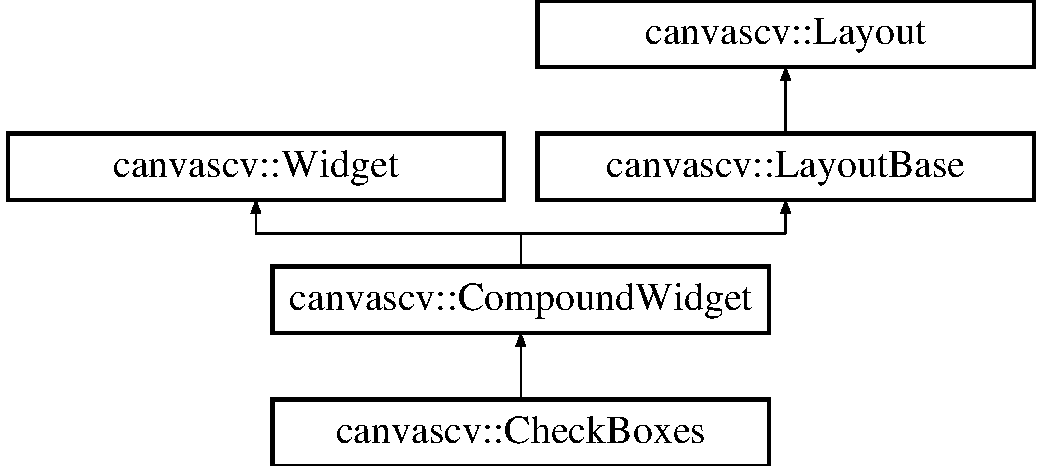
\includegraphics[height=4.000000cm]{classcanvascv_1_1CheckBoxes}
\end{center}
\end{figure}
\subsection*{Public Member Functions}
\begin{DoxyCompactItemize}
\item 
void \hyperlink{classcanvascv_1_1CheckBoxes_ae5614e44017cd8e7169448a9ea3269ec}{set\+Checked} (int index, bool checked)
\begin{DoxyCompactList}\small\item\em set\+Selection \end{DoxyCompactList}\item 
bool \hyperlink{classcanvascv_1_1CheckBoxes_a2e544c7f81248c6b297460be5852506e}{is\+Checked} (int index) const 
\begin{DoxyCompactList}\small\item\em is\+Checked \end{DoxyCompactList}\item 
std\+::string \hyperlink{classcanvascv_1_1CheckBoxes_a1ca004ddd840090415924b1f79b2ee47}{get\+Text\+At} (int index) const 
\begin{DoxyCompactList}\small\item\em get\+Text\+At \end{DoxyCompactList}\item 
size\+\_\+t \hyperlink{classcanvascv_1_1CheckBoxes_ac2e93b64ec078504230c7330d068248c}{size} () const \hypertarget{classcanvascv_1_1CheckBoxes_ac2e93b64ec078504230c7330d068248c}{}\label{classcanvascv_1_1CheckBoxes_ac2e93b64ec078504230c7330d068248c}

\begin{DoxyCompactList}\small\item\em return nunmber of check boxes in group \end{DoxyCompactList}\item 
void \hyperlink{classcanvascv_1_1CheckBoxes_a940fd899b9d206d4d2fc41b309bd0423}{set\+User\+CB} (\hyperlink{classcanvascv_1_1Widget_a977cbd39cf203c5866f07f3645c7e4bc}{Widget\+::\+C\+B\+User\+Selection} cb\+User\+Selection)\hypertarget{classcanvascv_1_1CheckBoxes_a940fd899b9d206d4d2fc41b309bd0423}{}\label{classcanvascv_1_1CheckBoxes_a940fd899b9d206d4d2fc41b309bd0423}

\begin{DoxyCompactList}\small\item\em cb\+User\+Selection will be invoked per user selection \end{DoxyCompactList}\item 
virtual const char $\ast$ \hyperlink{classcanvascv_1_1CheckBoxes_a59d8af71b4304f97f9caa178d38c99be}{get\+Type} () const 
\begin{DoxyCompactList}\small\item\em get\+Type is always implemented by derived to return the same static pointer per widget. \end{DoxyCompactList}\end{DoxyCompactItemize}
\subsection*{Static Public Member Functions}
\begin{DoxyCompactItemize}
\item 
static std\+::shared\+\_\+ptr$<$ \hyperlink{classcanvascv_1_1CheckBoxes}{Check\+Boxes} $>$ \hyperlink{classcanvascv_1_1CheckBoxes_a5108f52385a5cb19ad7fe52a18a91df0}{create} (\hyperlink{classcanvascv_1_1Layout}{Layout} \&layout\+Val, std\+::vector$<$ std\+::string $>$ check\+Box\+Names, \hyperlink{classcanvascv_1_1Widget_a977cbd39cf203c5866f07f3645c7e4bc}{Widget\+::\+C\+B\+User\+Selection} cb\+User\+Selection=\hyperlink{classcanvascv_1_1Widget_a977cbd39cf203c5866f07f3645c7e4bc}{Widget\+::\+C\+B\+User\+Selection}(), const cv\+::\+Point \&pos=cv\+::\+Point(0, 0))
\begin{DoxyCompactList}\small\item\em create a check box widget \end{DoxyCompactList}\end{DoxyCompactItemize}
\subsection*{Protected Member Functions}
\begin{DoxyCompactItemize}
\item 
virtual void \hyperlink{classcanvascv_1_1CheckBoxes_a50cae1ae73c9d69f864bc7fe6d6fedd6}{recalc\+Compound} ()
\begin{DoxyCompactList}\small\item\em recalc\+Compound \end{DoxyCompactList}\end{DoxyCompactItemize}
\subsection*{Additional Inherited Members}


\subsection{Detailed Description}
Use a check box to get a user selection for multiple options \begin{Desc}
\item[Examples\+: ]\par
\hyperlink{example_checkboxes_8cpp-example}{example\+\_\+checkboxes.\+cpp}.\end{Desc}


\subsection{Member Function Documentation}
\index{canvascv\+::\+Check\+Boxes@{canvascv\+::\+Check\+Boxes}!create@{create}}
\index{create@{create}!canvascv\+::\+Check\+Boxes@{canvascv\+::\+Check\+Boxes}}
\subsubsection[{\texorpdfstring{create(\+Layout \&layout\+Val, std\+::vector$<$ std\+::string $>$ check\+Box\+Names, Widget\+::\+C\+B\+User\+Selection cb\+User\+Selection=\+Widget\+::\+C\+B\+User\+Selection(), const cv\+::\+Point \&pos=cv\+::\+Point(0, 0))}{create(Layout &layoutVal, std::vector< std::string > checkBoxNames, Widget::CBUserSelection cbUserSelection=Widget::CBUserSelection(), const cv::Point &pos=cv::Point(0, 0))}}]{\setlength{\rightskip}{0pt plus 5cm}static std\+::shared\+\_\+ptr$<${\bf Check\+Boxes}$>$ canvascv\+::\+Check\+Boxes\+::create (
\begin{DoxyParamCaption}
\item[{{\bf Layout} \&}]{layout\+Val, }
\item[{std\+::vector$<$ std\+::string $>$}]{check\+Box\+Names, }
\item[{{\bf Widget\+::\+C\+B\+User\+Selection}}]{cb\+User\+Selection = {\ttfamily {\bf Widget\+::\+C\+B\+User\+Selection}()}, }
\item[{const cv\+::\+Point \&}]{pos = {\ttfamily cv\+:\+:Point(0,~0)}}
\end{DoxyParamCaption}
)\hspace{0.3cm}{\ttfamily [static]}}\hypertarget{classcanvascv_1_1CheckBoxes_a5108f52385a5cb19ad7fe52a18a91df0}{}\label{classcanvascv_1_1CheckBoxes_a5108f52385a5cb19ad7fe52a18a91df0}

\begin{DoxyParams}{Parameters}
{\em layout\+Val} & widgets are placed in layouts Canvas/\+V\+Frame/\+H\+Frame/... \\
\hline
{\em check\+Box\+Names} & automatically create items with names of check\+Box\+Names \\
\hline
{\em cb\+User\+Selection} & a callback to invoke with index of pressed check\+Box \\
\hline
{\em pos} & location in the \hyperlink{classcanvascv_1_1Layout}{Layout} (if the layout supports Point locations) \\
\hline
\end{DoxyParams}
\begin{DoxyReturn}{Returns}
a smart pointer copy of the object kept in the \hyperlink{classcanvascv_1_1Layout}{Layout} 
\begin{DoxyCode}
Canvas c(winName, image.size());
\textcolor{keyword}{auto} selectionBoxes = \hyperlink{classcanvascv_1_1CheckBoxes_a5108f52385a5cb19ad7fe52a18a91df0}{CheckBoxes::create}(c, \{
                                        \textcolor{stringliteral}{"Long Option1"},     \textcolor{comment}{// index 0}
                                        \textcolor{stringliteral}{"Option2\(\backslash\)n2 lines"}, \textcolor{comment}{// index 1}
                                        \textcolor{stringliteral}{"Option3"}           \textcolor{comment}{// index 2}
                                    \},
                                    [](Widget *w, \textcolor{keywordtype}{int} i) \{
    w->setVisible(\textcolor{keyword}{false});
    cout << \textcolor{stringliteral}{"Option "} << i << \textcolor{stringliteral}{" was chosen"} << endl;
\});
\textcolor{keywordflow}{while}(...)
\{
    c.\hyperlink{classcanvascv_1_1Canvas_a018c66e277de7904b8146ea3f3feebdd}{redrawOn}(...);
    imshow(...);
    key = c.\hyperlink{classcanvascv_1_1Canvas_a59397db05f5d9e45264f626f6a2ae528}{waitKeyEx}(...); \textcolor{comment}{// GUI and callbacks happen here}
\}
\end{DoxyCode}
 
\end{DoxyReturn}
\begin{Desc}
\item[Examples\+: ]\par
\hyperlink{example_checkboxes_8cpp-example}{example\+\_\+checkboxes.\+cpp}.\end{Desc}
\index{canvascv\+::\+Check\+Boxes@{canvascv\+::\+Check\+Boxes}!get\+Text\+At@{get\+Text\+At}}
\index{get\+Text\+At@{get\+Text\+At}!canvascv\+::\+Check\+Boxes@{canvascv\+::\+Check\+Boxes}}
\subsubsection[{\texorpdfstring{get\+Text\+At(int index) const }{getTextAt(int index) const }}]{\setlength{\rightskip}{0pt plus 5cm}std\+::string canvascv\+::\+Check\+Boxes\+::get\+Text\+At (
\begin{DoxyParamCaption}
\item[{int}]{index}
\end{DoxyParamCaption}
) const}\hypertarget{classcanvascv_1_1CheckBoxes_a1ca004ddd840090415924b1f79b2ee47}{}\label{classcanvascv_1_1CheckBoxes_a1ca004ddd840090415924b1f79b2ee47}
return the text at index index 
\begin{DoxyParams}{Parameters}
{\em index} & is the index you want the text for \\
\hline
\end{DoxyParams}
\begin{DoxyReturn}{Returns}
return the text at index index or empty string if invalid index 
\end{DoxyReturn}
\begin{Desc}
\item[Examples\+: ]\par
\hyperlink{example_checkboxes_8cpp-example}{example\+\_\+checkboxes.\+cpp}.\end{Desc}
\index{canvascv\+::\+Check\+Boxes@{canvascv\+::\+Check\+Boxes}!get\+Type@{get\+Type}}
\index{get\+Type@{get\+Type}!canvascv\+::\+Check\+Boxes@{canvascv\+::\+Check\+Boxes}}
\subsubsection[{\texorpdfstring{get\+Type() const }{getType() const }}]{\setlength{\rightskip}{0pt plus 5cm}virtual const char$\ast$ canvascv\+::\+Check\+Boxes\+::get\+Type (
\begin{DoxyParamCaption}
{}
\end{DoxyParamCaption}
) const\hspace{0.3cm}{\ttfamily [virtual]}}\hypertarget{classcanvascv_1_1CheckBoxes_a59d8af71b4304f97f9caa178d38c99be}{}\label{classcanvascv_1_1CheckBoxes_a59d8af71b4304f97f9caa178d38c99be}
\begin{DoxyReturn}{Returns}
const char $\ast$ pointer to string with widget type name 
\end{DoxyReturn}


Implements \hyperlink{classcanvascv_1_1Widget_a85884269bd53ab91203f099a586efa43}{canvascv\+::\+Widget}.

\index{canvascv\+::\+Check\+Boxes@{canvascv\+::\+Check\+Boxes}!is\+Checked@{is\+Checked}}
\index{is\+Checked@{is\+Checked}!canvascv\+::\+Check\+Boxes@{canvascv\+::\+Check\+Boxes}}
\subsubsection[{\texorpdfstring{is\+Checked(int index) const }{isChecked(int index) const }}]{\setlength{\rightskip}{0pt plus 5cm}bool canvascv\+::\+Check\+Boxes\+::is\+Checked (
\begin{DoxyParamCaption}
\item[{int}]{index}
\end{DoxyParamCaption}
) const}\hypertarget{classcanvascv_1_1CheckBoxes_a2e544c7f81248c6b297460be5852506e}{}\label{classcanvascv_1_1CheckBoxes_a2e544c7f81248c6b297460be5852506e}
is a box at index checked 
\begin{DoxyParams}{Parameters}
{\em index} & is box index \\
\hline
\end{DoxyParams}
\begin{DoxyReturn}{Returns}
true or flase for checked or unchecked 
\end{DoxyReturn}
\begin{Desc}
\item[Examples\+: ]\par
\hyperlink{example_checkboxes_8cpp-example}{example\+\_\+checkboxes.\+cpp}.\end{Desc}
\index{canvascv\+::\+Check\+Boxes@{canvascv\+::\+Check\+Boxes}!recalc\+Compound@{recalc\+Compound}}
\index{recalc\+Compound@{recalc\+Compound}!canvascv\+::\+Check\+Boxes@{canvascv\+::\+Check\+Boxes}}
\subsubsection[{\texorpdfstring{recalc\+Compound()}{recalcCompound()}}]{\setlength{\rightskip}{0pt plus 5cm}virtual void canvascv\+::\+Check\+Boxes\+::recalc\+Compound (
\begin{DoxyParamCaption}
{}
\end{DoxyParamCaption}
)\hspace{0.3cm}{\ttfamily [protected]}, {\ttfamily [virtual]}}\hypertarget{classcanvascv_1_1CheckBoxes_a50cae1ae73c9d69f864bc7fe6d6fedd6}{}\label{classcanvascv_1_1CheckBoxes_a50cae1ae73c9d69f864bc7fe6d6fedd6}
Your BG size recalculation/allocation and FG drawing is done here. It is done semi automatically. Is you invoke setters in this method on your internal widgets, then make sure to update them and/or their layout 

Implements \hyperlink{classcanvascv_1_1CompoundWidget_a4a4f8241d6fd187ffcae2c7968f13864}{canvascv\+::\+Compound\+Widget}.

\index{canvascv\+::\+Check\+Boxes@{canvascv\+::\+Check\+Boxes}!set\+Checked@{set\+Checked}}
\index{set\+Checked@{set\+Checked}!canvascv\+::\+Check\+Boxes@{canvascv\+::\+Check\+Boxes}}
\subsubsection[{\texorpdfstring{set\+Checked(int index, bool checked)}{setChecked(int index, bool checked)}}]{\setlength{\rightskip}{0pt plus 5cm}void canvascv\+::\+Check\+Boxes\+::set\+Checked (
\begin{DoxyParamCaption}
\item[{int}]{index, }
\item[{bool}]{checked}
\end{DoxyParamCaption}
)}\hypertarget{classcanvascv_1_1CheckBoxes_ae5614e44017cd8e7169448a9ea3269ec}{}\label{classcanvascv_1_1CheckBoxes_ae5614e44017cd8e7169448a9ea3269ec}
make a certain box checked 
\begin{DoxyParams}{Parameters}
{\em index} & is box index \\
\hline
{\em checked} & is true or false for checked or unchecked \\
\hline
\end{DoxyParams}


The documentation for this class was generated from the following file\+:\begin{DoxyCompactItemize}
\item 
Canvas\+C\+V-\/doxygen/src/canvascv/widgets/checkboxes.\+h\end{DoxyCompactItemize}

\hypertarget{classcanvascv_1_1Colors}{}\section{canvascv\+:\+:Colors Class Reference}
\label{classcanvascv_1_1Colors}\index{canvascv\+::\+Colors@{canvascv\+::\+Colors}}


The \hyperlink{classcanvascv_1_1Colors}{Colors} class.  




{\ttfamily \#include $<$colors.\+h$>$}

\subsection*{Static Public Attributes}
\begin{DoxyCompactItemize}
\item 
static const cv\+::\+Scalar \hyperlink{classcanvascv_1_1Colors_a8ce831ec6123adb0a5504fc515f15c72}{O\+P\+A\+Q\+UE}\hypertarget{classcanvascv_1_1Colors_a8ce831ec6123adb0a5504fc515f15c72}{}\label{classcanvascv_1_1Colors_a8ce831ec6123adb0a5504fc515f15c72}

\begin{DoxyCompactList}\small\item\em can be added to other colors \end{DoxyCompactList}\item 
static const cv\+::\+Scalar \hyperlink{classcanvascv_1_1Colors_afcf2e7359a45b54affb1d2c4df47730f}{T\+R\+A\+N\+S\+P\+A\+R\+E\+NT}\hypertarget{classcanvascv_1_1Colors_afcf2e7359a45b54affb1d2c4df47730f}{}\label{classcanvascv_1_1Colors_afcf2e7359a45b54affb1d2c4df47730f}

\begin{DoxyCompactList}\small\item\em can be added to other colors \end{DoxyCompactList}\item 
static const cv\+::\+Scalar \hyperlink{classcanvascv_1_1Colors_acb99327f0cf205bd37f5687d89ddec20}{Maroon}\hypertarget{classcanvascv_1_1Colors_acb99327f0cf205bd37f5687d89ddec20}{}\label{classcanvascv_1_1Colors_acb99327f0cf205bd37f5687d89ddec20}

\begin{DoxyCompactList}\small\item\em ~~ R\+GB\+: (128,0,0) H\+EX\+: \#800000 \end{DoxyCompactList}\item 
static const cv\+::\+Scalar \hyperlink{classcanvascv_1_1Colors_a29a1cd16453b2d75bdb4324b395f2796}{Dark\+Red}\hypertarget{classcanvascv_1_1Colors_a29a1cd16453b2d75bdb4324b395f2796}{}\label{classcanvascv_1_1Colors_a29a1cd16453b2d75bdb4324b395f2796}

\begin{DoxyCompactList}\small\item\em ~~ R\+GB\+: (139,0,0) H\+EX\+: \#8\+B0000 \end{DoxyCompactList}\item 
static const cv\+::\+Scalar \hyperlink{classcanvascv_1_1Colors_a30753a55b55b1798265d0ea9be44f7ca}{Brown}\hypertarget{classcanvascv_1_1Colors_a30753a55b55b1798265d0ea9be44f7ca}{}\label{classcanvascv_1_1Colors_a30753a55b55b1798265d0ea9be44f7ca}

\begin{DoxyCompactList}\small\item\em ~~ R\+GB\+: (165,42,42) H\+EX\+: \#\+A52\+A2A \end{DoxyCompactList}\item 
static const cv\+::\+Scalar \hyperlink{classcanvascv_1_1Colors_a9ad88cce0936f36c820a0942008ea0b7}{Firebrick}\hypertarget{classcanvascv_1_1Colors_a9ad88cce0936f36c820a0942008ea0b7}{}\label{classcanvascv_1_1Colors_a9ad88cce0936f36c820a0942008ea0b7}

\begin{DoxyCompactList}\small\item\em ~~ R\+GB\+: (178,34,34) H\+EX\+: \#\+B22222 \end{DoxyCompactList}\item 
static const cv\+::\+Scalar \hyperlink{classcanvascv_1_1Colors_a0ea3ae498dcd6dd86f3a2b1cffe23b26}{Crimson}\hypertarget{classcanvascv_1_1Colors_a0ea3ae498dcd6dd86f3a2b1cffe23b26}{}\label{classcanvascv_1_1Colors_a0ea3ae498dcd6dd86f3a2b1cffe23b26}

\begin{DoxyCompactList}\small\item\em ~~ R\+GB\+: (220,20,60) H\+EX\+: \#\+D\+C143C \end{DoxyCompactList}\item 
static const cv\+::\+Scalar \hyperlink{classcanvascv_1_1Colors_a10aff24c53edf45b038d0636b061f9c2}{Red}\hypertarget{classcanvascv_1_1Colors_a10aff24c53edf45b038d0636b061f9c2}{}\label{classcanvascv_1_1Colors_a10aff24c53edf45b038d0636b061f9c2}

\begin{DoxyCompactList}\small\item\em ~~ R\+GB\+: (255,0,0) H\+EX\+: \#\+F\+F0000 \end{DoxyCompactList}\item 
static const cv\+::\+Scalar \hyperlink{classcanvascv_1_1Colors_a07faee5fa36ce572e41255b05d442e99}{Tomato}\hypertarget{classcanvascv_1_1Colors_a07faee5fa36ce572e41255b05d442e99}{}\label{classcanvascv_1_1Colors_a07faee5fa36ce572e41255b05d442e99}

\begin{DoxyCompactList}\small\item\em ~~ R\+GB\+: (255,99,71) H\+EX\+: \#\+F\+F6347 \end{DoxyCompactList}\item 
static const cv\+::\+Scalar \hyperlink{classcanvascv_1_1Colors_a6635b8af8ff9745c0903cdbeb8901bf9}{Coral}\hypertarget{classcanvascv_1_1Colors_a6635b8af8ff9745c0903cdbeb8901bf9}{}\label{classcanvascv_1_1Colors_a6635b8af8ff9745c0903cdbeb8901bf9}

\begin{DoxyCompactList}\small\item\em ~~ R\+GB\+: (255,127,80) H\+EX\+: \#\+F\+F7\+F50 \end{DoxyCompactList}\item 
static const cv\+::\+Scalar \hyperlink{classcanvascv_1_1Colors_a525b441478da213c870396f2c422dcef}{Indian\+Red}\hypertarget{classcanvascv_1_1Colors_a525b441478da213c870396f2c422dcef}{}\label{classcanvascv_1_1Colors_a525b441478da213c870396f2c422dcef}

\begin{DoxyCompactList}\small\item\em ~~ R\+GB\+: (205,92,92) H\+EX\+: \#\+C\+D5\+C5C \end{DoxyCompactList}\item 
static const cv\+::\+Scalar \hyperlink{classcanvascv_1_1Colors_a327d0081cce9e8790721cb7fb5477511}{Light\+Coral}\hypertarget{classcanvascv_1_1Colors_a327d0081cce9e8790721cb7fb5477511}{}\label{classcanvascv_1_1Colors_a327d0081cce9e8790721cb7fb5477511}

\begin{DoxyCompactList}\small\item\em ~~ R\+GB\+: (240,128,128) H\+EX\+: \#\+F08080 \end{DoxyCompactList}\item 
static const cv\+::\+Scalar \hyperlink{classcanvascv_1_1Colors_a1d3a826928f24172701289b736bc3fd3}{Dark\+Salmon}\hypertarget{classcanvascv_1_1Colors_a1d3a826928f24172701289b736bc3fd3}{}\label{classcanvascv_1_1Colors_a1d3a826928f24172701289b736bc3fd3}

\begin{DoxyCompactList}\small\item\em ~~ R\+GB\+: (233,150,122) H\+EX\+: \#\+E9967A \end{DoxyCompactList}\item 
static const cv\+::\+Scalar \hyperlink{classcanvascv_1_1Colors_aeecdcae36abf9c0a5cad0f80c24ef485}{Salmon}\hypertarget{classcanvascv_1_1Colors_aeecdcae36abf9c0a5cad0f80c24ef485}{}\label{classcanvascv_1_1Colors_aeecdcae36abf9c0a5cad0f80c24ef485}

\begin{DoxyCompactList}\small\item\em ~~ R\+GB\+: (250,128,114) H\+EX\+: \#\+F\+A8072 \end{DoxyCompactList}\item 
static const cv\+::\+Scalar \hyperlink{classcanvascv_1_1Colors_a39315a311cfc672daafce66a259efc64}{Light\+Salmon}\hypertarget{classcanvascv_1_1Colors_a39315a311cfc672daafce66a259efc64}{}\label{classcanvascv_1_1Colors_a39315a311cfc672daafce66a259efc64}

\begin{DoxyCompactList}\small\item\em ~~ R\+GB\+: (255,160,122) H\+EX\+: \#\+F\+F\+A07A \end{DoxyCompactList}\item 
static const cv\+::\+Scalar \hyperlink{classcanvascv_1_1Colors_a3d259d4f4dfa7ec396abb053c8cb74cc}{Orange\+Red}\hypertarget{classcanvascv_1_1Colors_a3d259d4f4dfa7ec396abb053c8cb74cc}{}\label{classcanvascv_1_1Colors_a3d259d4f4dfa7ec396abb053c8cb74cc}

\begin{DoxyCompactList}\small\item\em ~~ R\+GB\+: (255,69,0) H\+EX\+: \#\+F\+F4500 \end{DoxyCompactList}\item 
static const cv\+::\+Scalar \hyperlink{classcanvascv_1_1Colors_a8b14aa892e77d94b86548ee54774d226}{Dark\+Orange}\hypertarget{classcanvascv_1_1Colors_a8b14aa892e77d94b86548ee54774d226}{}\label{classcanvascv_1_1Colors_a8b14aa892e77d94b86548ee54774d226}

\begin{DoxyCompactList}\small\item\em ~~ R\+GB\+: (255,140,0) H\+EX\+: \#\+F\+F8\+C00 \end{DoxyCompactList}\item 
static const cv\+::\+Scalar \hyperlink{classcanvascv_1_1Colors_a463fb59b35fb56e7a4eaa5976baaa411}{Orange}\hypertarget{classcanvascv_1_1Colors_a463fb59b35fb56e7a4eaa5976baaa411}{}\label{classcanvascv_1_1Colors_a463fb59b35fb56e7a4eaa5976baaa411}

\begin{DoxyCompactList}\small\item\em ~~ R\+GB\+: (255,165,0) H\+EX\+: \#\+F\+F\+A500 \end{DoxyCompactList}\item 
static const cv\+::\+Scalar \hyperlink{classcanvascv_1_1Colors_a14db295c402b60a93306c09f3e605467}{Gold}\hypertarget{classcanvascv_1_1Colors_a14db295c402b60a93306c09f3e605467}{}\label{classcanvascv_1_1Colors_a14db295c402b60a93306c09f3e605467}

\begin{DoxyCompactList}\small\item\em ~~ R\+GB\+: (255,215,0) H\+EX\+: \#\+F\+F\+D700 \end{DoxyCompactList}\item 
static const cv\+::\+Scalar \hyperlink{classcanvascv_1_1Colors_a693dabc1911a039a0e03d799beb1d41e}{Dark\+Golden\+Rod}\hypertarget{classcanvascv_1_1Colors_a693dabc1911a039a0e03d799beb1d41e}{}\label{classcanvascv_1_1Colors_a693dabc1911a039a0e03d799beb1d41e}

\begin{DoxyCompactList}\small\item\em ~~ R\+GB\+: (184,134,11) H\+EX\+: \#\+B8860B \end{DoxyCompactList}\item 
static const cv\+::\+Scalar \hyperlink{classcanvascv_1_1Colors_a3a58c44a1725a798b07ea4e2ccf1c220}{Golden\+Rod}\hypertarget{classcanvascv_1_1Colors_a3a58c44a1725a798b07ea4e2ccf1c220}{}\label{classcanvascv_1_1Colors_a3a58c44a1725a798b07ea4e2ccf1c220}

\begin{DoxyCompactList}\small\item\em ~~ R\+GB\+: (218,165,32) H\+EX\+: \#\+D\+A\+A520 \end{DoxyCompactList}\item 
static const cv\+::\+Scalar \hyperlink{classcanvascv_1_1Colors_a4f6c8acb35d839810e5c15648c5026a3}{Pale\+Golden\+Rod}\hypertarget{classcanvascv_1_1Colors_a4f6c8acb35d839810e5c15648c5026a3}{}\label{classcanvascv_1_1Colors_a4f6c8acb35d839810e5c15648c5026a3}

\begin{DoxyCompactList}\small\item\em ~~ R\+GB\+: (238,232,170) H\+EX\+: \#\+E\+E\+E8\+AA \end{DoxyCompactList}\item 
static const cv\+::\+Scalar \hyperlink{classcanvascv_1_1Colors_ad4a5d9248452a5aa5f91f406e00c035c}{Dark\+Khaki}\hypertarget{classcanvascv_1_1Colors_ad4a5d9248452a5aa5f91f406e00c035c}{}\label{classcanvascv_1_1Colors_ad4a5d9248452a5aa5f91f406e00c035c}

\begin{DoxyCompactList}\small\item\em ~~ R\+GB\+: (189,183,107) H\+EX\+: \#\+B\+D\+B76B \end{DoxyCompactList}\item 
static const cv\+::\+Scalar \hyperlink{classcanvascv_1_1Colors_a5e7e7dacf95d084b0a2f1e51f7ffc395}{Khaki}\hypertarget{classcanvascv_1_1Colors_a5e7e7dacf95d084b0a2f1e51f7ffc395}{}\label{classcanvascv_1_1Colors_a5e7e7dacf95d084b0a2f1e51f7ffc395}

\begin{DoxyCompactList}\small\item\em ~~ R\+GB\+: (240,230,140) H\+EX\+: \#\+F0\+E68C \end{DoxyCompactList}\item 
static const cv\+::\+Scalar \hyperlink{classcanvascv_1_1Colors_afb7b1c0683abcd39c97e4ba542f87172}{Olive}\hypertarget{classcanvascv_1_1Colors_afb7b1c0683abcd39c97e4ba542f87172}{}\label{classcanvascv_1_1Colors_afb7b1c0683abcd39c97e4ba542f87172}

\begin{DoxyCompactList}\small\item\em ~~ R\+GB\+: (128,128,0) H\+EX\+: \#808000 \end{DoxyCompactList}\item 
static const cv\+::\+Scalar \hyperlink{classcanvascv_1_1Colors_a92d369430d9d2436d45a34dff7b7bde8}{Yellow}\hypertarget{classcanvascv_1_1Colors_a92d369430d9d2436d45a34dff7b7bde8}{}\label{classcanvascv_1_1Colors_a92d369430d9d2436d45a34dff7b7bde8}

\begin{DoxyCompactList}\small\item\em ~~ R\+GB\+: (255,255,0) H\+EX\+: \#\+F\+F\+F\+F00 \end{DoxyCompactList}\item 
static const cv\+::\+Scalar \hyperlink{classcanvascv_1_1Colors_a00d0dd747f88c0b54818136af1038051}{Yellow\+Green}\hypertarget{classcanvascv_1_1Colors_a00d0dd747f88c0b54818136af1038051}{}\label{classcanvascv_1_1Colors_a00d0dd747f88c0b54818136af1038051}

\begin{DoxyCompactList}\small\item\em ~~ R\+GB\+: (154,205,50) H\+EX\+: \#9\+A\+C\+D32 \end{DoxyCompactList}\item 
static const cv\+::\+Scalar \hyperlink{classcanvascv_1_1Colors_a6fc99c0e07f0e56d91215438b32d368f}{Dark\+Olive\+Green}\hypertarget{classcanvascv_1_1Colors_a6fc99c0e07f0e56d91215438b32d368f}{}\label{classcanvascv_1_1Colors_a6fc99c0e07f0e56d91215438b32d368f}

\begin{DoxyCompactList}\small\item\em ~~ R\+GB\+: (85,107,47) H\+EX\+: \#556\+B2F \end{DoxyCompactList}\item 
static const cv\+::\+Scalar \hyperlink{classcanvascv_1_1Colors_a9543f13ad0145ccfbc2427a12898a40e}{Olive\+Drab}\hypertarget{classcanvascv_1_1Colors_a9543f13ad0145ccfbc2427a12898a40e}{}\label{classcanvascv_1_1Colors_a9543f13ad0145ccfbc2427a12898a40e}

\begin{DoxyCompactList}\small\item\em ~~ R\+GB\+: (107,142,35) H\+EX\+: \#6\+B8\+E23 \end{DoxyCompactList}\item 
static const cv\+::\+Scalar \hyperlink{classcanvascv_1_1Colors_a453e4e18b5f8b9e933f3cfb228757c81}{Lawn\+Green}\hypertarget{classcanvascv_1_1Colors_a453e4e18b5f8b9e933f3cfb228757c81}{}\label{classcanvascv_1_1Colors_a453e4e18b5f8b9e933f3cfb228757c81}

\begin{DoxyCompactList}\small\item\em ~~ R\+GB\+: (124,252,0) H\+EX\+: \#7\+C\+F\+C00 \end{DoxyCompactList}\item 
static const cv\+::\+Scalar \hyperlink{classcanvascv_1_1Colors_abfcdf0a760e45bd969686647de1f4c6b}{Chart\+Reuse}\hypertarget{classcanvascv_1_1Colors_abfcdf0a760e45bd969686647de1f4c6b}{}\label{classcanvascv_1_1Colors_abfcdf0a760e45bd969686647de1f4c6b}

\begin{DoxyCompactList}\small\item\em ~~ R\+GB\+: (127,255,0) H\+EX\+: \#7\+F\+F\+F00 \end{DoxyCompactList}\item 
static const cv\+::\+Scalar \hyperlink{classcanvascv_1_1Colors_a5c670b91d2875ec9f0c789ed7eddafc0}{Green\+Yellow}\hypertarget{classcanvascv_1_1Colors_a5c670b91d2875ec9f0c789ed7eddafc0}{}\label{classcanvascv_1_1Colors_a5c670b91d2875ec9f0c789ed7eddafc0}

\begin{DoxyCompactList}\small\item\em ~~ R\+GB\+: (173,255,47) H\+EX\+: \#\+A\+D\+F\+F2F \end{DoxyCompactList}\item 
static const cv\+::\+Scalar \hyperlink{classcanvascv_1_1Colors_acbd7ca16f07b5ff69f3f370951f061c8}{Dark\+Green}\hypertarget{classcanvascv_1_1Colors_acbd7ca16f07b5ff69f3f370951f061c8}{}\label{classcanvascv_1_1Colors_acbd7ca16f07b5ff69f3f370951f061c8}

\begin{DoxyCompactList}\small\item\em ~~ R\+GB\+: (0,100,0) H\+EX\+: \#006400 \end{DoxyCompactList}\item 
static const cv\+::\+Scalar \hyperlink{classcanvascv_1_1Colors_a93c492d5ea68350ee63d5b91315b5ea7}{Green}\hypertarget{classcanvascv_1_1Colors_a93c492d5ea68350ee63d5b91315b5ea7}{}\label{classcanvascv_1_1Colors_a93c492d5ea68350ee63d5b91315b5ea7}

\begin{DoxyCompactList}\small\item\em ~~ R\+GB\+: (0,128,0) H\+EX\+: \#008000 \end{DoxyCompactList}\item 
static const cv\+::\+Scalar \hyperlink{classcanvascv_1_1Colors_a886b107535e8ab3461d9b2d2b7e5a73c}{Forest\+Green}\hypertarget{classcanvascv_1_1Colors_a886b107535e8ab3461d9b2d2b7e5a73c}{}\label{classcanvascv_1_1Colors_a886b107535e8ab3461d9b2d2b7e5a73c}

\begin{DoxyCompactList}\small\item\em ~~ R\+GB\+: (34,139,34) H\+EX\+: \#228\+B22 \end{DoxyCompactList}\item 
static const cv\+::\+Scalar \hyperlink{classcanvascv_1_1Colors_a3212fe8ea3dc44c6fa68866f5217ba25}{Lime}\hypertarget{classcanvascv_1_1Colors_a3212fe8ea3dc44c6fa68866f5217ba25}{}\label{classcanvascv_1_1Colors_a3212fe8ea3dc44c6fa68866f5217ba25}

\begin{DoxyCompactList}\small\item\em ~~ R\+GB\+: (0,255,0) H\+EX\+: \#00\+F\+F00 \end{DoxyCompactList}\item 
static const cv\+::\+Scalar \hyperlink{classcanvascv_1_1Colors_a82ccef73fa5e513117fc7940f2681004}{Lime\+Green}\hypertarget{classcanvascv_1_1Colors_a82ccef73fa5e513117fc7940f2681004}{}\label{classcanvascv_1_1Colors_a82ccef73fa5e513117fc7940f2681004}

\begin{DoxyCompactList}\small\item\em ~~ R\+GB\+: (50,205,50) H\+EX\+: \#32\+C\+D32 \end{DoxyCompactList}\item 
static const cv\+::\+Scalar \hyperlink{classcanvascv_1_1Colors_a1f9941ac0c2677c2d346e78fbde8f3fe}{Light\+Green}\hypertarget{classcanvascv_1_1Colors_a1f9941ac0c2677c2d346e78fbde8f3fe}{}\label{classcanvascv_1_1Colors_a1f9941ac0c2677c2d346e78fbde8f3fe}

\begin{DoxyCompactList}\small\item\em ~~ R\+GB\+: (144,238,144) H\+EX\+: \#90\+E\+E90 \end{DoxyCompactList}\item 
static const cv\+::\+Scalar \hyperlink{classcanvascv_1_1Colors_a106e6b72b0a9be84da291d20ea6b86b9}{Pale\+Green}\hypertarget{classcanvascv_1_1Colors_a106e6b72b0a9be84da291d20ea6b86b9}{}\label{classcanvascv_1_1Colors_a106e6b72b0a9be84da291d20ea6b86b9}

\begin{DoxyCompactList}\small\item\em ~~ R\+GB\+: (152,251,152) H\+EX\+: \#98\+F\+B98 \end{DoxyCompactList}\item 
static const cv\+::\+Scalar \hyperlink{classcanvascv_1_1Colors_a94cfb2b88c10f848cb90d41fc70ac973}{Dark\+Sea\+Green}\hypertarget{classcanvascv_1_1Colors_a94cfb2b88c10f848cb90d41fc70ac973}{}\label{classcanvascv_1_1Colors_a94cfb2b88c10f848cb90d41fc70ac973}

\begin{DoxyCompactList}\small\item\em ~~ R\+GB\+: (143,188,143) H\+EX\+: \#8\+F\+B\+C8F \end{DoxyCompactList}\item 
static const cv\+::\+Scalar \hyperlink{classcanvascv_1_1Colors_a14b53e9c352337feb4776a868d265ed6}{Medium\+Spring\+Green}\hypertarget{classcanvascv_1_1Colors_a14b53e9c352337feb4776a868d265ed6}{}\label{classcanvascv_1_1Colors_a14b53e9c352337feb4776a868d265ed6}

\begin{DoxyCompactList}\small\item\em ~~ R\+GB\+: (0,250,154) H\+EX\+: \#00\+F\+A9A \end{DoxyCompactList}\item 
static const cv\+::\+Scalar \hyperlink{classcanvascv_1_1Colors_a6b3f1c0fed7b8bab92b0cd2576b9b56f}{Spring\+Green}\hypertarget{classcanvascv_1_1Colors_a6b3f1c0fed7b8bab92b0cd2576b9b56f}{}\label{classcanvascv_1_1Colors_a6b3f1c0fed7b8bab92b0cd2576b9b56f}

\begin{DoxyCompactList}\small\item\em ~~ R\+GB\+: (0,255,127) H\+EX\+: \#00\+F\+F7F \end{DoxyCompactList}\item 
static const cv\+::\+Scalar \hyperlink{classcanvascv_1_1Colors_a6f174f3d9ca64eae5ddbf0fa4621231e}{Sea\+Green}\hypertarget{classcanvascv_1_1Colors_a6f174f3d9ca64eae5ddbf0fa4621231e}{}\label{classcanvascv_1_1Colors_a6f174f3d9ca64eae5ddbf0fa4621231e}

\begin{DoxyCompactList}\small\item\em ~~ R\+GB\+: (46,139,87) H\+EX\+: \#2\+E8\+B57 \end{DoxyCompactList}\item 
static const cv\+::\+Scalar \hyperlink{classcanvascv_1_1Colors_a610e1866a7ea7aed27c24c0e3599b2c6}{Medium\+Aqua\+Marine}\hypertarget{classcanvascv_1_1Colors_a610e1866a7ea7aed27c24c0e3599b2c6}{}\label{classcanvascv_1_1Colors_a610e1866a7ea7aed27c24c0e3599b2c6}

\begin{DoxyCompactList}\small\item\em ~~ R\+GB\+: (102,205,170) H\+EX\+: \#66\+C\+D\+AA \end{DoxyCompactList}\item 
static const cv\+::\+Scalar \hyperlink{classcanvascv_1_1Colors_a624f5f14354588d4c729f9cd66d56103}{Medium\+Sea\+Green}\hypertarget{classcanvascv_1_1Colors_a624f5f14354588d4c729f9cd66d56103}{}\label{classcanvascv_1_1Colors_a624f5f14354588d4c729f9cd66d56103}

\begin{DoxyCompactList}\small\item\em ~~ R\+GB\+: (60,179,113) H\+EX\+: \#3\+C\+B371 \end{DoxyCompactList}\item 
static const cv\+::\+Scalar \hyperlink{classcanvascv_1_1Colors_aa2f72c17921fa5c893860fae6e4fdfc4}{Light\+Sea\+Green}\hypertarget{classcanvascv_1_1Colors_aa2f72c17921fa5c893860fae6e4fdfc4}{}\label{classcanvascv_1_1Colors_aa2f72c17921fa5c893860fae6e4fdfc4}

\begin{DoxyCompactList}\small\item\em ~~ R\+GB\+: (32,178,170) H\+EX\+: \#20\+B2\+AA \end{DoxyCompactList}\item 
static const cv\+::\+Scalar \hyperlink{classcanvascv_1_1Colors_ac66e6a923be591fb68570281286c7c05}{Dark\+Slate\+Gray}\hypertarget{classcanvascv_1_1Colors_ac66e6a923be591fb68570281286c7c05}{}\label{classcanvascv_1_1Colors_ac66e6a923be591fb68570281286c7c05}

\begin{DoxyCompactList}\small\item\em ~~ R\+GB\+: (47,79,79) H\+EX\+: \#2\+F4\+F4F \end{DoxyCompactList}\item 
static const cv\+::\+Scalar \hyperlink{classcanvascv_1_1Colors_a739bf703aca32d6ba82f871cff4edf10}{Teal}\hypertarget{classcanvascv_1_1Colors_a739bf703aca32d6ba82f871cff4edf10}{}\label{classcanvascv_1_1Colors_a739bf703aca32d6ba82f871cff4edf10}

\begin{DoxyCompactList}\small\item\em ~~ R\+GB\+: (0,128,128) H\+EX\+: \#008080 \end{DoxyCompactList}\item 
static const cv\+::\+Scalar \hyperlink{classcanvascv_1_1Colors_a8eaa68747a618e95e56cfc61d3e25f07}{Dark\+Cyan}\hypertarget{classcanvascv_1_1Colors_a8eaa68747a618e95e56cfc61d3e25f07}{}\label{classcanvascv_1_1Colors_a8eaa68747a618e95e56cfc61d3e25f07}

\begin{DoxyCompactList}\small\item\em ~~ R\+GB\+: (0,139,139) H\+EX\+: \#008\+B8B \end{DoxyCompactList}\item 
static const cv\+::\+Scalar \hyperlink{classcanvascv_1_1Colors_a1e18e84141ad99d86fdf133b70a6d47c}{Aqua}\hypertarget{classcanvascv_1_1Colors_a1e18e84141ad99d86fdf133b70a6d47c}{}\label{classcanvascv_1_1Colors_a1e18e84141ad99d86fdf133b70a6d47c}

\begin{DoxyCompactList}\small\item\em ~~ R\+GB\+: (0,255,255) H\+EX\+: \#00\+F\+F\+FF \end{DoxyCompactList}\item 
static const cv\+::\+Scalar \hyperlink{classcanvascv_1_1Colors_a5bb20fa77dd40915ce6949e7531f925c}{Cyan}\hypertarget{classcanvascv_1_1Colors_a5bb20fa77dd40915ce6949e7531f925c}{}\label{classcanvascv_1_1Colors_a5bb20fa77dd40915ce6949e7531f925c}

\begin{DoxyCompactList}\small\item\em ~~ R\+GB\+: (0,255,255) H\+EX\+: \#00\+F\+F\+FF \end{DoxyCompactList}\item 
static const cv\+::\+Scalar \hyperlink{classcanvascv_1_1Colors_a2133be4670f8c4cf45f1851feb792cbd}{Light\+Cyan}\hypertarget{classcanvascv_1_1Colors_a2133be4670f8c4cf45f1851feb792cbd}{}\label{classcanvascv_1_1Colors_a2133be4670f8c4cf45f1851feb792cbd}

\begin{DoxyCompactList}\small\item\em ~~ R\+GB\+: (224,255,255) H\+EX\+: \#\+E0\+F\+F\+FF \end{DoxyCompactList}\item 
static const cv\+::\+Scalar \hyperlink{classcanvascv_1_1Colors_a7f095f9f4b95e3d2443ad6cf67757d32}{Dark\+Turquoise}\hypertarget{classcanvascv_1_1Colors_a7f095f9f4b95e3d2443ad6cf67757d32}{}\label{classcanvascv_1_1Colors_a7f095f9f4b95e3d2443ad6cf67757d32}

\begin{DoxyCompactList}\small\item\em ~~ R\+GB\+: (0,206,209) H\+EX\+: \#00\+C\+E\+D1 \end{DoxyCompactList}\item 
static const cv\+::\+Scalar \hyperlink{classcanvascv_1_1Colors_a1634d6dbb7d8ababfe789402e09ec616}{Turquoise}\hypertarget{classcanvascv_1_1Colors_a1634d6dbb7d8ababfe789402e09ec616}{}\label{classcanvascv_1_1Colors_a1634d6dbb7d8ababfe789402e09ec616}

\begin{DoxyCompactList}\small\item\em ~~ R\+GB\+: (64,224,208) H\+EX\+: \#40\+E0\+D0 \end{DoxyCompactList}\item 
static const cv\+::\+Scalar \hyperlink{classcanvascv_1_1Colors_a8a89589625633b662742e10ff04c3315}{Medium\+Turquoise}\hypertarget{classcanvascv_1_1Colors_a8a89589625633b662742e10ff04c3315}{}\label{classcanvascv_1_1Colors_a8a89589625633b662742e10ff04c3315}

\begin{DoxyCompactList}\small\item\em ~~ R\+GB\+: (72,209,204) H\+EX\+: \#48\+D1\+CC \end{DoxyCompactList}\item 
static const cv\+::\+Scalar \hyperlink{classcanvascv_1_1Colors_ad3e7880020e9d94b2772daba5477e400}{Pale\+Turquoise}\hypertarget{classcanvascv_1_1Colors_ad3e7880020e9d94b2772daba5477e400}{}\label{classcanvascv_1_1Colors_ad3e7880020e9d94b2772daba5477e400}

\begin{DoxyCompactList}\small\item\em ~~ R\+GB\+: (175,238,238) H\+EX\+: \#\+A\+F\+E\+E\+EE \end{DoxyCompactList}\item 
static const cv\+::\+Scalar \hyperlink{classcanvascv_1_1Colors_afff6b965ad68a6dd820718fc15bcfb72}{Aqua\+Marine}\hypertarget{classcanvascv_1_1Colors_afff6b965ad68a6dd820718fc15bcfb72}{}\label{classcanvascv_1_1Colors_afff6b965ad68a6dd820718fc15bcfb72}

\begin{DoxyCompactList}\small\item\em ~~ R\+GB\+: (127,255,212) H\+EX\+: \#7\+F\+F\+F\+D4 \end{DoxyCompactList}\item 
static const cv\+::\+Scalar \hyperlink{classcanvascv_1_1Colors_a7fc255f9a1b3271e4b2e89ffdbd77a3e}{Powder\+Blue}\hypertarget{classcanvascv_1_1Colors_a7fc255f9a1b3271e4b2e89ffdbd77a3e}{}\label{classcanvascv_1_1Colors_a7fc255f9a1b3271e4b2e89ffdbd77a3e}

\begin{DoxyCompactList}\small\item\em ~~ R\+GB\+: (176,224,230) H\+EX\+: \#\+B0\+E0\+E6 \end{DoxyCompactList}\item 
static const cv\+::\+Scalar \hyperlink{classcanvascv_1_1Colors_aa13abe6a87f845ca8b9ca6422c93b341}{Cadet\+Blue}\hypertarget{classcanvascv_1_1Colors_aa13abe6a87f845ca8b9ca6422c93b341}{}\label{classcanvascv_1_1Colors_aa13abe6a87f845ca8b9ca6422c93b341}

\begin{DoxyCompactList}\small\item\em ~~ R\+GB\+: (95,158,160) H\+EX\+: \#5\+F9\+E\+A0 \end{DoxyCompactList}\item 
static const cv\+::\+Scalar \hyperlink{classcanvascv_1_1Colors_ad126676b619c3cd83b37d390144b81d6}{Steel\+Blue}\hypertarget{classcanvascv_1_1Colors_ad126676b619c3cd83b37d390144b81d6}{}\label{classcanvascv_1_1Colors_ad126676b619c3cd83b37d390144b81d6}

\begin{DoxyCompactList}\small\item\em ~~ R\+GB\+: (70,130,180) H\+EX\+: \#4682\+B4 \end{DoxyCompactList}\item 
static const cv\+::\+Scalar \hyperlink{classcanvascv_1_1Colors_a002b1335f384990794a04a56cef92959}{Corn\+Flower\+Blue}\hypertarget{classcanvascv_1_1Colors_a002b1335f384990794a04a56cef92959}{}\label{classcanvascv_1_1Colors_a002b1335f384990794a04a56cef92959}

\begin{DoxyCompactList}\small\item\em ~~ R\+GB\+: (100,149,237) H\+EX\+: \#6495\+ED \end{DoxyCompactList}\item 
static const cv\+::\+Scalar \hyperlink{classcanvascv_1_1Colors_a32106ce8f118e33a24a2c5f3048e6cd7}{Deep\+Sky\+Blue}\hypertarget{classcanvascv_1_1Colors_a32106ce8f118e33a24a2c5f3048e6cd7}{}\label{classcanvascv_1_1Colors_a32106ce8f118e33a24a2c5f3048e6cd7}

\begin{DoxyCompactList}\small\item\em ~~ R\+GB\+: (0,191,255) H\+EX\+: \#00\+B\+F\+FF \end{DoxyCompactList}\item 
static const cv\+::\+Scalar \hyperlink{classcanvascv_1_1Colors_a43b0172f931d81a957a172035966b8fa}{Dodger\+Blue}\hypertarget{classcanvascv_1_1Colors_a43b0172f931d81a957a172035966b8fa}{}\label{classcanvascv_1_1Colors_a43b0172f931d81a957a172035966b8fa}

\begin{DoxyCompactList}\small\item\em ~~ R\+GB\+: (30,144,255) H\+EX\+: \#1\+E90\+FF \end{DoxyCompactList}\item 
static const cv\+::\+Scalar \hyperlink{classcanvascv_1_1Colors_a48011d22ca034494ebd4af882edec154}{Light\+Blue}\hypertarget{classcanvascv_1_1Colors_a48011d22ca034494ebd4af882edec154}{}\label{classcanvascv_1_1Colors_a48011d22ca034494ebd4af882edec154}

\begin{DoxyCompactList}\small\item\em ~~ R\+GB\+: (173,216,230) H\+EX\+: \#\+A\+D\+D8\+E6 \end{DoxyCompactList}\item 
static const cv\+::\+Scalar \hyperlink{classcanvascv_1_1Colors_a86c13cd4b9a4c13831177623f70afb15}{Sky\+Blue}\hypertarget{classcanvascv_1_1Colors_a86c13cd4b9a4c13831177623f70afb15}{}\label{classcanvascv_1_1Colors_a86c13cd4b9a4c13831177623f70afb15}

\begin{DoxyCompactList}\small\item\em ~~ R\+GB\+: (135,206,235) H\+EX\+: \#87\+C\+E\+EB \end{DoxyCompactList}\item 
static const cv\+::\+Scalar \hyperlink{classcanvascv_1_1Colors_ad5adec81f45c8698e02480a3b801da56}{Light\+Sky\+Blue}\hypertarget{classcanvascv_1_1Colors_ad5adec81f45c8698e02480a3b801da56}{}\label{classcanvascv_1_1Colors_ad5adec81f45c8698e02480a3b801da56}

\begin{DoxyCompactList}\small\item\em ~~ R\+GB\+: (135,206,250) H\+EX\+: \#87\+C\+E\+FA \end{DoxyCompactList}\item 
static const cv\+::\+Scalar \hyperlink{classcanvascv_1_1Colors_ad02a085f60e38f4e5792674d76aff5ba}{Midnight\+Blue}\hypertarget{classcanvascv_1_1Colors_ad02a085f60e38f4e5792674d76aff5ba}{}\label{classcanvascv_1_1Colors_ad02a085f60e38f4e5792674d76aff5ba}

\begin{DoxyCompactList}\small\item\em ~~ R\+GB\+: (25,25,112) H\+EX\+: \#191970 \end{DoxyCompactList}\item 
static const cv\+::\+Scalar \hyperlink{classcanvascv_1_1Colors_a8a504bdb43bb7bf9b14e60de4b38d7a4}{Navy}\hypertarget{classcanvascv_1_1Colors_a8a504bdb43bb7bf9b14e60de4b38d7a4}{}\label{classcanvascv_1_1Colors_a8a504bdb43bb7bf9b14e60de4b38d7a4}

\begin{DoxyCompactList}\small\item\em ~~ R\+GB\+: (0,0,128) H\+EX\+: \#000080 \end{DoxyCompactList}\item 
static const cv\+::\+Scalar \hyperlink{classcanvascv_1_1Colors_a719690c9780f154593064e8c638ca8ed}{Dark\+Blue}\hypertarget{classcanvascv_1_1Colors_a719690c9780f154593064e8c638ca8ed}{}\label{classcanvascv_1_1Colors_a719690c9780f154593064e8c638ca8ed}

\begin{DoxyCompactList}\small\item\em ~~ R\+GB\+: (0,0,139) H\+EX\+: \#00008B \end{DoxyCompactList}\item 
static const cv\+::\+Scalar \hyperlink{classcanvascv_1_1Colors_a7b52ba1c8bcf608a0dabb9cc6319f43e}{Medium\+Blue}\hypertarget{classcanvascv_1_1Colors_a7b52ba1c8bcf608a0dabb9cc6319f43e}{}\label{classcanvascv_1_1Colors_a7b52ba1c8bcf608a0dabb9cc6319f43e}

\begin{DoxyCompactList}\small\item\em ~~ R\+GB\+: (0,0,205) H\+EX\+: \#0000\+CD \end{DoxyCompactList}\item 
static const cv\+::\+Scalar \hyperlink{classcanvascv_1_1Colors_a2a48572768ea2c3912a1a5c8de4f1954}{Blue}\hypertarget{classcanvascv_1_1Colors_a2a48572768ea2c3912a1a5c8de4f1954}{}\label{classcanvascv_1_1Colors_a2a48572768ea2c3912a1a5c8de4f1954}

\begin{DoxyCompactList}\small\item\em ~~ R\+GB\+: (0,0,255) H\+EX\+: \#0000\+FF \end{DoxyCompactList}\item 
static const cv\+::\+Scalar \hyperlink{classcanvascv_1_1Colors_acabb2042568dac2c0fbefcc92b48be0b}{Royal\+Blue}\hypertarget{classcanvascv_1_1Colors_acabb2042568dac2c0fbefcc92b48be0b}{}\label{classcanvascv_1_1Colors_acabb2042568dac2c0fbefcc92b48be0b}

\begin{DoxyCompactList}\small\item\em ~~ R\+GB\+: (65,105,225) H\+EX\+: \#4169\+E1 \end{DoxyCompactList}\item 
static const cv\+::\+Scalar \hyperlink{classcanvascv_1_1Colors_ae3e38807167fc22eb6929f54f7b5358e}{Blue\+Violet}\hypertarget{classcanvascv_1_1Colors_ae3e38807167fc22eb6929f54f7b5358e}{}\label{classcanvascv_1_1Colors_ae3e38807167fc22eb6929f54f7b5358e}

\begin{DoxyCompactList}\small\item\em ~~ R\+GB\+: (138,43,226) H\+EX\+: \#8\+A2\+B\+E2 \end{DoxyCompactList}\item 
static const cv\+::\+Scalar \hyperlink{classcanvascv_1_1Colors_ace69296b502904c57c3930cf432db858}{Indigo}\hypertarget{classcanvascv_1_1Colors_ace69296b502904c57c3930cf432db858}{}\label{classcanvascv_1_1Colors_ace69296b502904c57c3930cf432db858}

\begin{DoxyCompactList}\small\item\em ~~ R\+GB\+: (75,0,130) H\+EX\+: \#4\+B0082 \end{DoxyCompactList}\item 
static const cv\+::\+Scalar \hyperlink{classcanvascv_1_1Colors_ac20afd846ec87e7bdf9cc38c1c6755ba}{Dark\+Slate\+Blue}\hypertarget{classcanvascv_1_1Colors_ac20afd846ec87e7bdf9cc38c1c6755ba}{}\label{classcanvascv_1_1Colors_ac20afd846ec87e7bdf9cc38c1c6755ba}

\begin{DoxyCompactList}\small\item\em ~~ R\+GB\+: (72,61,139) H\+EX\+: \#483\+D8B \end{DoxyCompactList}\item 
static const cv\+::\+Scalar \hyperlink{classcanvascv_1_1Colors_ab95931f06bf0e363976219f00f38dc65}{Slate\+Blue}\hypertarget{classcanvascv_1_1Colors_ab95931f06bf0e363976219f00f38dc65}{}\label{classcanvascv_1_1Colors_ab95931f06bf0e363976219f00f38dc65}

\begin{DoxyCompactList}\small\item\em ~~ R\+GB\+: (106,90,205) H\+EX\+: \#6\+A5\+A\+CD \end{DoxyCompactList}\item 
static const cv\+::\+Scalar \hyperlink{classcanvascv_1_1Colors_a429a3009cc342de6203b7589e036def0}{Medium\+Slate\+Blue}\hypertarget{classcanvascv_1_1Colors_a429a3009cc342de6203b7589e036def0}{}\label{classcanvascv_1_1Colors_a429a3009cc342de6203b7589e036def0}

\begin{DoxyCompactList}\small\item\em ~~ R\+GB\+: (123,104,238) H\+EX\+: \#7\+B68\+EE \end{DoxyCompactList}\item 
static const cv\+::\+Scalar \hyperlink{classcanvascv_1_1Colors_a74712381a18f01741b83f6907c1426d2}{Medium\+Purple}\hypertarget{classcanvascv_1_1Colors_a74712381a18f01741b83f6907c1426d2}{}\label{classcanvascv_1_1Colors_a74712381a18f01741b83f6907c1426d2}

\begin{DoxyCompactList}\small\item\em ~~ R\+GB\+: (147,112,219) H\+EX\+: \#9370\+DB \end{DoxyCompactList}\item 
static const cv\+::\+Scalar \hyperlink{classcanvascv_1_1Colors_a4d36a8fd5dda17b145b1eecd97116fe2}{Dark\+Magenta}\hypertarget{classcanvascv_1_1Colors_a4d36a8fd5dda17b145b1eecd97116fe2}{}\label{classcanvascv_1_1Colors_a4d36a8fd5dda17b145b1eecd97116fe2}

\begin{DoxyCompactList}\small\item\em ~~ R\+GB\+: (139,0,139) H\+EX\+: \#8\+B008B \end{DoxyCompactList}\item 
static const cv\+::\+Scalar \hyperlink{classcanvascv_1_1Colors_a36da5ac0b100032fa3e0298d5950d32a}{Dark\+Violet}\hypertarget{classcanvascv_1_1Colors_a36da5ac0b100032fa3e0298d5950d32a}{}\label{classcanvascv_1_1Colors_a36da5ac0b100032fa3e0298d5950d32a}

\begin{DoxyCompactList}\small\item\em ~~ R\+GB\+: (148,0,211) H\+EX\+: \#9400\+D3 \end{DoxyCompactList}\item 
static const cv\+::\+Scalar \hyperlink{classcanvascv_1_1Colors_a92b4e5ffd1fba8499445819712595eb3}{Dark\+Orchid}\hypertarget{classcanvascv_1_1Colors_a92b4e5ffd1fba8499445819712595eb3}{}\label{classcanvascv_1_1Colors_a92b4e5ffd1fba8499445819712595eb3}

\begin{DoxyCompactList}\small\item\em ~~ R\+GB\+: (153,50,204) H\+EX\+: \#9932\+CC \end{DoxyCompactList}\item 
static const cv\+::\+Scalar \hyperlink{classcanvascv_1_1Colors_ae14078311181d06d36cac8cb40fc7571}{Medium\+Orchid}\hypertarget{classcanvascv_1_1Colors_ae14078311181d06d36cac8cb40fc7571}{}\label{classcanvascv_1_1Colors_ae14078311181d06d36cac8cb40fc7571}

\begin{DoxyCompactList}\small\item\em ~~ R\+GB\+: (186,85,211) H\+EX\+: \#\+B\+A55\+D3 \end{DoxyCompactList}\item 
static const cv\+::\+Scalar \hyperlink{classcanvascv_1_1Colors_a4b9e0c791c30e6a5bd9dd553ba609e78}{Purple}\hypertarget{classcanvascv_1_1Colors_a4b9e0c791c30e6a5bd9dd553ba609e78}{}\label{classcanvascv_1_1Colors_a4b9e0c791c30e6a5bd9dd553ba609e78}

\begin{DoxyCompactList}\small\item\em ~~ R\+GB\+: (128,0,128) H\+EX\+: \#800080 \end{DoxyCompactList}\item 
static const cv\+::\+Scalar \hyperlink{classcanvascv_1_1Colors_aa391df2a13b457cdd1c4ec693b3817a7}{Thistle}\hypertarget{classcanvascv_1_1Colors_aa391df2a13b457cdd1c4ec693b3817a7}{}\label{classcanvascv_1_1Colors_aa391df2a13b457cdd1c4ec693b3817a7}

\begin{DoxyCompactList}\small\item\em ~~ R\+GB\+: (216,191,216) H\+EX\+: \#\+D8\+B\+F\+D8 \end{DoxyCompactList}\item 
static const cv\+::\+Scalar \hyperlink{classcanvascv_1_1Colors_a86f8046c82086c08153f4f4ea80d41ad}{Plum}\hypertarget{classcanvascv_1_1Colors_a86f8046c82086c08153f4f4ea80d41ad}{}\label{classcanvascv_1_1Colors_a86f8046c82086c08153f4f4ea80d41ad}

\begin{DoxyCompactList}\small\item\em ~~ R\+GB\+: (221,160,221) H\+EX\+: \#\+D\+D\+A0\+DD \end{DoxyCompactList}\item 
static const cv\+::\+Scalar \hyperlink{classcanvascv_1_1Colors_aa460c32e69aeb81d3d3962d3d17106f3}{Violet}\hypertarget{classcanvascv_1_1Colors_aa460c32e69aeb81d3d3962d3d17106f3}{}\label{classcanvascv_1_1Colors_aa460c32e69aeb81d3d3962d3d17106f3}

\begin{DoxyCompactList}\small\item\em ~~ R\+GB\+: (238,130,238) H\+EX\+: \#\+E\+E82\+EE \end{DoxyCompactList}\item 
static const cv\+::\+Scalar \hyperlink{classcanvascv_1_1Colors_ad03cf7c8527fb8ea6c6d70b948894a12}{Magenta}\hypertarget{classcanvascv_1_1Colors_ad03cf7c8527fb8ea6c6d70b948894a12}{}\label{classcanvascv_1_1Colors_ad03cf7c8527fb8ea6c6d70b948894a12}

\begin{DoxyCompactList}\small\item\em ~~ R\+GB\+: (255,0,255) H\+EX\+: \#\+F\+F00\+FF \end{DoxyCompactList}\item 
static const cv\+::\+Scalar \hyperlink{classcanvascv_1_1Colors_ab0839cde478ab21af7741dee228192b4}{Fuchsia}\hypertarget{classcanvascv_1_1Colors_ab0839cde478ab21af7741dee228192b4}{}\label{classcanvascv_1_1Colors_ab0839cde478ab21af7741dee228192b4}

\begin{DoxyCompactList}\small\item\em ~~ R\+GB\+: (255,0,255) H\+EX\+: \#\+F\+F00\+FF \end{DoxyCompactList}\item 
static const cv\+::\+Scalar \hyperlink{classcanvascv_1_1Colors_a8eac7074ead796201ad2e5fcd7b37f55}{Orchid}\hypertarget{classcanvascv_1_1Colors_a8eac7074ead796201ad2e5fcd7b37f55}{}\label{classcanvascv_1_1Colors_a8eac7074ead796201ad2e5fcd7b37f55}

\begin{DoxyCompactList}\small\item\em ~~ R\+GB\+: (218,112,214) H\+EX\+: \#\+D\+A70\+D6 \end{DoxyCompactList}\item 
static const cv\+::\+Scalar \hyperlink{classcanvascv_1_1Colors_aeef7356ae9ddce20ad7a7653ff7f1319}{Medium\+Violet\+Red}\hypertarget{classcanvascv_1_1Colors_aeef7356ae9ddce20ad7a7653ff7f1319}{}\label{classcanvascv_1_1Colors_aeef7356ae9ddce20ad7a7653ff7f1319}

\begin{DoxyCompactList}\small\item\em ~~ R\+GB\+: (199,21,133) H\+EX\+: \#\+C71585 \end{DoxyCompactList}\item 
static const cv\+::\+Scalar \hyperlink{classcanvascv_1_1Colors_a7ba1b0dc2d489c51ddc7d0b7feb8d1d0}{Pale\+Violet\+Red}\hypertarget{classcanvascv_1_1Colors_a7ba1b0dc2d489c51ddc7d0b7feb8d1d0}{}\label{classcanvascv_1_1Colors_a7ba1b0dc2d489c51ddc7d0b7feb8d1d0}

\begin{DoxyCompactList}\small\item\em ~~ R\+GB\+: (219,112,147) H\+EX\+: \#\+D\+B7093 \end{DoxyCompactList}\item 
static const cv\+::\+Scalar \hyperlink{classcanvascv_1_1Colors_a9a83f4b13795374abb0a6dd4361f6ddb}{Deep\+Pink}\hypertarget{classcanvascv_1_1Colors_a9a83f4b13795374abb0a6dd4361f6ddb}{}\label{classcanvascv_1_1Colors_a9a83f4b13795374abb0a6dd4361f6ddb}

\begin{DoxyCompactList}\small\item\em ~~ R\+GB\+: (255,20,147) H\+EX\+: \#\+F\+F1493 \end{DoxyCompactList}\item 
static const cv\+::\+Scalar \hyperlink{classcanvascv_1_1Colors_af790e812a0f8e32106173e9c06f13f5f}{Hot\+Pink}\hypertarget{classcanvascv_1_1Colors_af790e812a0f8e32106173e9c06f13f5f}{}\label{classcanvascv_1_1Colors_af790e812a0f8e32106173e9c06f13f5f}

\begin{DoxyCompactList}\small\item\em ~~ R\+GB\+: (255,105,180) H\+EX\+: \#\+F\+F69\+B4 \end{DoxyCompactList}\item 
static const cv\+::\+Scalar \hyperlink{classcanvascv_1_1Colors_aee87ec44916305fcf1b9c8758213c2d8}{Light\+Pink}\hypertarget{classcanvascv_1_1Colors_aee87ec44916305fcf1b9c8758213c2d8}{}\label{classcanvascv_1_1Colors_aee87ec44916305fcf1b9c8758213c2d8}

\begin{DoxyCompactList}\small\item\em ~~ R\+GB\+: (255,182,193) H\+EX\+: \#\+F\+F\+B6\+C1 \end{DoxyCompactList}\item 
static const cv\+::\+Scalar \hyperlink{classcanvascv_1_1Colors_a85747d82637552b830d926f913aecb25}{Pink}\hypertarget{classcanvascv_1_1Colors_a85747d82637552b830d926f913aecb25}{}\label{classcanvascv_1_1Colors_a85747d82637552b830d926f913aecb25}

\begin{DoxyCompactList}\small\item\em ~~ R\+GB\+: (255,192,203) H\+EX\+: \#\+F\+F\+C0\+CB \end{DoxyCompactList}\item 
static const cv\+::\+Scalar \hyperlink{classcanvascv_1_1Colors_a76ffd50a1f955552099cd09965174367}{Antique\+White}\hypertarget{classcanvascv_1_1Colors_a76ffd50a1f955552099cd09965174367}{}\label{classcanvascv_1_1Colors_a76ffd50a1f955552099cd09965174367}

\begin{DoxyCompactList}\small\item\em ~~ R\+GB\+: (250,235,215) H\+EX\+: \#\+F\+A\+E\+B\+D7 \end{DoxyCompactList}\item 
static const cv\+::\+Scalar \hyperlink{classcanvascv_1_1Colors_ad2533524d2924906a8f3611f81dc6ffe}{Beige}\hypertarget{classcanvascv_1_1Colors_ad2533524d2924906a8f3611f81dc6ffe}{}\label{classcanvascv_1_1Colors_ad2533524d2924906a8f3611f81dc6ffe}

\begin{DoxyCompactList}\small\item\em ~~ R\+GB\+: (245,245,220) H\+EX\+: \#\+F5\+F5\+DC \end{DoxyCompactList}\item 
static const cv\+::\+Scalar \hyperlink{classcanvascv_1_1Colors_a6e56124a4455f69d1250a001524d70e2}{Bisque}\hypertarget{classcanvascv_1_1Colors_a6e56124a4455f69d1250a001524d70e2}{}\label{classcanvascv_1_1Colors_a6e56124a4455f69d1250a001524d70e2}

\begin{DoxyCompactList}\small\item\em ~~ R\+GB\+: (255,228,196) H\+EX\+: \#\+F\+F\+E4\+C4 \end{DoxyCompactList}\item 
static const cv\+::\+Scalar \hyperlink{classcanvascv_1_1Colors_a45eff66ca768534448da8739773b761d}{Blanched\+Almond}\hypertarget{classcanvascv_1_1Colors_a45eff66ca768534448da8739773b761d}{}\label{classcanvascv_1_1Colors_a45eff66ca768534448da8739773b761d}

\begin{DoxyCompactList}\small\item\em ~~ R\+GB\+: (255,235,205) H\+EX\+: \#\+F\+F\+E\+B\+CD \end{DoxyCompactList}\item 
static const cv\+::\+Scalar \hyperlink{classcanvascv_1_1Colors_abdf1b5b05df103dd98f0ece1a6e3719e}{Wheat}\hypertarget{classcanvascv_1_1Colors_abdf1b5b05df103dd98f0ece1a6e3719e}{}\label{classcanvascv_1_1Colors_abdf1b5b05df103dd98f0ece1a6e3719e}

\begin{DoxyCompactList}\small\item\em ~~ R\+GB\+: (245,222,179) H\+EX\+: \#\+F5\+D\+E\+B3 \end{DoxyCompactList}\item 
static const cv\+::\+Scalar \hyperlink{classcanvascv_1_1Colors_ae3c14894ce951c52ae5ad0b8f7f57bfc}{Corn\+Silk}\hypertarget{classcanvascv_1_1Colors_ae3c14894ce951c52ae5ad0b8f7f57bfc}{}\label{classcanvascv_1_1Colors_ae3c14894ce951c52ae5ad0b8f7f57bfc}

\begin{DoxyCompactList}\small\item\em ~~ R\+GB\+: (255,248,220) H\+EX\+: \#\+F\+F\+F8\+DC \end{DoxyCompactList}\item 
static const cv\+::\+Scalar \hyperlink{classcanvascv_1_1Colors_ad04b3f94f885606d167a4e4c8480e97c}{Lemon\+Chiffon}\hypertarget{classcanvascv_1_1Colors_ad04b3f94f885606d167a4e4c8480e97c}{}\label{classcanvascv_1_1Colors_ad04b3f94f885606d167a4e4c8480e97c}

\begin{DoxyCompactList}\small\item\em ~~ R\+GB\+: (255,250,205) H\+EX\+: \#\+F\+F\+F\+A\+CD \end{DoxyCompactList}\item 
static const cv\+::\+Scalar \hyperlink{classcanvascv_1_1Colors_a8b2919184b567020ab06f3fb428773cf}{Light\+Golden\+Rod\+Yellow}\hypertarget{classcanvascv_1_1Colors_a8b2919184b567020ab06f3fb428773cf}{}\label{classcanvascv_1_1Colors_a8b2919184b567020ab06f3fb428773cf}

\begin{DoxyCompactList}\small\item\em ~~ R\+GB\+: (250,250,210) H\+EX\+: \#\+F\+A\+F\+A\+D2 \end{DoxyCompactList}\item 
static const cv\+::\+Scalar \hyperlink{classcanvascv_1_1Colors_a6e2b95c2ef4ca3e4d536670e2091e21a}{Light\+Yellow}\hypertarget{classcanvascv_1_1Colors_a6e2b95c2ef4ca3e4d536670e2091e21a}{}\label{classcanvascv_1_1Colors_a6e2b95c2ef4ca3e4d536670e2091e21a}

\begin{DoxyCompactList}\small\item\em ~~ R\+GB\+: (255,255,224) H\+EX\+: \#\+F\+F\+F\+F\+E0 \end{DoxyCompactList}\item 
static const cv\+::\+Scalar \hyperlink{classcanvascv_1_1Colors_a9ce71fe6b5a49bb951c301062d84aa5c}{Saddle\+Brown}\hypertarget{classcanvascv_1_1Colors_a9ce71fe6b5a49bb951c301062d84aa5c}{}\label{classcanvascv_1_1Colors_a9ce71fe6b5a49bb951c301062d84aa5c}

\begin{DoxyCompactList}\small\item\em ~~ R\+GB\+: (139,69,19) H\+EX\+: \#8\+B4513 \end{DoxyCompactList}\item 
static const cv\+::\+Scalar \hyperlink{classcanvascv_1_1Colors_ab0d950de7f52bcdb182de73acfedbc45}{Sienna}\hypertarget{classcanvascv_1_1Colors_ab0d950de7f52bcdb182de73acfedbc45}{}\label{classcanvascv_1_1Colors_ab0d950de7f52bcdb182de73acfedbc45}

\begin{DoxyCompactList}\small\item\em ~~ R\+GB\+: (160,82,45) H\+EX\+: \#\+A0522D \end{DoxyCompactList}\item 
static const cv\+::\+Scalar \hyperlink{classcanvascv_1_1Colors_a0b50c3da054db3443093d62cf0de5004}{Chocolate}\hypertarget{classcanvascv_1_1Colors_a0b50c3da054db3443093d62cf0de5004}{}\label{classcanvascv_1_1Colors_a0b50c3da054db3443093d62cf0de5004}

\begin{DoxyCompactList}\small\item\em ~~ R\+GB\+: (210,105,30) H\+EX\+: \#\+D2691E \end{DoxyCompactList}\item 
static const cv\+::\+Scalar \hyperlink{classcanvascv_1_1Colors_a7e18fbb34046b99f8875ad6ab6c17175}{Peru}\hypertarget{classcanvascv_1_1Colors_a7e18fbb34046b99f8875ad6ab6c17175}{}\label{classcanvascv_1_1Colors_a7e18fbb34046b99f8875ad6ab6c17175}

\begin{DoxyCompactList}\small\item\em ~~ R\+GB\+: (205,133,63) H\+EX\+: \#\+C\+D853F \end{DoxyCompactList}\item 
static const cv\+::\+Scalar \hyperlink{classcanvascv_1_1Colors_a2f8549bf1e8867f800bfe83e35bce727}{Sandy\+Brown}\hypertarget{classcanvascv_1_1Colors_a2f8549bf1e8867f800bfe83e35bce727}{}\label{classcanvascv_1_1Colors_a2f8549bf1e8867f800bfe83e35bce727}

\begin{DoxyCompactList}\small\item\em ~~ R\+GB\+: (244,164,96) H\+EX\+: \#\+F4\+A460 \end{DoxyCompactList}\item 
static const cv\+::\+Scalar \hyperlink{classcanvascv_1_1Colors_a8a0a8db10d7e919d758c15eb3c4fe879}{Burly\+Wood}\hypertarget{classcanvascv_1_1Colors_a8a0a8db10d7e919d758c15eb3c4fe879}{}\label{classcanvascv_1_1Colors_a8a0a8db10d7e919d758c15eb3c4fe879}

\begin{DoxyCompactList}\small\item\em ~~ R\+GB\+: (222,184,135) H\+EX\+: \#\+D\+E\+B887 \end{DoxyCompactList}\item 
static const cv\+::\+Scalar \hyperlink{classcanvascv_1_1Colors_acc9ba39ebb412fff2e76684d65aa7556}{Tan}\hypertarget{classcanvascv_1_1Colors_acc9ba39ebb412fff2e76684d65aa7556}{}\label{classcanvascv_1_1Colors_acc9ba39ebb412fff2e76684d65aa7556}

\begin{DoxyCompactList}\small\item\em ~~ R\+GB\+: (210,180,140) H\+EX\+: \#\+D2\+B48C \end{DoxyCompactList}\item 
static const cv\+::\+Scalar \hyperlink{classcanvascv_1_1Colors_a490b8f4293572c230f377968f6ed1252}{Rosy\+Brown}\hypertarget{classcanvascv_1_1Colors_a490b8f4293572c230f377968f6ed1252}{}\label{classcanvascv_1_1Colors_a490b8f4293572c230f377968f6ed1252}

\begin{DoxyCompactList}\small\item\em ~~ R\+GB\+: (188,143,143) H\+EX\+: \#\+B\+C8\+F8F \end{DoxyCompactList}\item 
static const cv\+::\+Scalar \hyperlink{classcanvascv_1_1Colors_a1acea719ec9c94894974ea212c100538}{Moccasin}\hypertarget{classcanvascv_1_1Colors_a1acea719ec9c94894974ea212c100538}{}\label{classcanvascv_1_1Colors_a1acea719ec9c94894974ea212c100538}

\begin{DoxyCompactList}\small\item\em ~~ R\+GB\+: (255,228,181) H\+EX\+: \#\+F\+F\+E4\+B5 \end{DoxyCompactList}\item 
static const cv\+::\+Scalar \hyperlink{classcanvascv_1_1Colors_ad6023f66caf3b7497a9c93c62276bf48}{Navajo\+White}\hypertarget{classcanvascv_1_1Colors_ad6023f66caf3b7497a9c93c62276bf48}{}\label{classcanvascv_1_1Colors_ad6023f66caf3b7497a9c93c62276bf48}

\begin{DoxyCompactList}\small\item\em ~~ R\+GB\+: (255,222,173) H\+EX\+: \#\+F\+F\+D\+E\+AD \end{DoxyCompactList}\item 
static const cv\+::\+Scalar \hyperlink{classcanvascv_1_1Colors_aea0e345484553a018d5b97bf8fe46fe1}{Peach\+Puff}\hypertarget{classcanvascv_1_1Colors_aea0e345484553a018d5b97bf8fe46fe1}{}\label{classcanvascv_1_1Colors_aea0e345484553a018d5b97bf8fe46fe1}

\begin{DoxyCompactList}\small\item\em ~~ R\+GB\+: (255,218,185) H\+EX\+: \#\+F\+F\+D\+A\+B9 \end{DoxyCompactList}\item 
static const cv\+::\+Scalar \hyperlink{classcanvascv_1_1Colors_a277faa63d1ed9df6c4b8be82b4e3622a}{Misty\+Rose}\hypertarget{classcanvascv_1_1Colors_a277faa63d1ed9df6c4b8be82b4e3622a}{}\label{classcanvascv_1_1Colors_a277faa63d1ed9df6c4b8be82b4e3622a}

\begin{DoxyCompactList}\small\item\em ~~ R\+GB\+: (255,228,225) H\+EX\+: \#\+F\+F\+E4\+E1 \end{DoxyCompactList}\item 
static const cv\+::\+Scalar \hyperlink{classcanvascv_1_1Colors_a04f21ff0f561ba6d472767db9e1e88dd}{Lavender\+Blush}\hypertarget{classcanvascv_1_1Colors_a04f21ff0f561ba6d472767db9e1e88dd}{}\label{classcanvascv_1_1Colors_a04f21ff0f561ba6d472767db9e1e88dd}

\begin{DoxyCompactList}\small\item\em ~~ R\+GB\+: (255,240,245) H\+EX\+: \#\+F\+F\+F0\+F5 \end{DoxyCompactList}\item 
static const cv\+::\+Scalar \hyperlink{classcanvascv_1_1Colors_aff2a0026b59d84d047be8097d6dba07f}{Linen}\hypertarget{classcanvascv_1_1Colors_aff2a0026b59d84d047be8097d6dba07f}{}\label{classcanvascv_1_1Colors_aff2a0026b59d84d047be8097d6dba07f}

\begin{DoxyCompactList}\small\item\em ~~ R\+GB\+: (250,240,230) H\+EX\+: \#\+F\+A\+F0\+E6 \end{DoxyCompactList}\item 
static const cv\+::\+Scalar \hyperlink{classcanvascv_1_1Colors_a5225bce8494ff90a68e431e71f0dd4c2}{Old\+Lace}\hypertarget{classcanvascv_1_1Colors_a5225bce8494ff90a68e431e71f0dd4c2}{}\label{classcanvascv_1_1Colors_a5225bce8494ff90a68e431e71f0dd4c2}

\begin{DoxyCompactList}\small\item\em ~~ R\+GB\+: (253,245,230) H\+EX\+: \#\+F\+D\+F5\+E6 \end{DoxyCompactList}\item 
static const cv\+::\+Scalar \hyperlink{classcanvascv_1_1Colors_ae229196cabbf7a4a9b046781623ee711}{Papaya\+Whip}\hypertarget{classcanvascv_1_1Colors_ae229196cabbf7a4a9b046781623ee711}{}\label{classcanvascv_1_1Colors_ae229196cabbf7a4a9b046781623ee711}

\begin{DoxyCompactList}\small\item\em ~~ R\+GB\+: (255,239,213) H\+EX\+: \#\+F\+F\+E\+F\+D5 \end{DoxyCompactList}\item 
static const cv\+::\+Scalar \hyperlink{classcanvascv_1_1Colors_a9f67ac0a9ea18d2e84a000f9fef29fb0}{Sea\+Shell}\hypertarget{classcanvascv_1_1Colors_a9f67ac0a9ea18d2e84a000f9fef29fb0}{}\label{classcanvascv_1_1Colors_a9f67ac0a9ea18d2e84a000f9fef29fb0}

\begin{DoxyCompactList}\small\item\em ~~ R\+GB\+: (255,245,238) H\+EX\+: \#\+F\+F\+F5\+EE \end{DoxyCompactList}\item 
static const cv\+::\+Scalar \hyperlink{classcanvascv_1_1Colors_abccad45ffeb78d1dbc62511ee23b3358}{Mint\+Cream}\hypertarget{classcanvascv_1_1Colors_abccad45ffeb78d1dbc62511ee23b3358}{}\label{classcanvascv_1_1Colors_abccad45ffeb78d1dbc62511ee23b3358}

\begin{DoxyCompactList}\small\item\em ~~ R\+GB\+: (245,255,250) H\+EX\+: \#\+F5\+F\+F\+FA \end{DoxyCompactList}\item 
static const cv\+::\+Scalar \hyperlink{classcanvascv_1_1Colors_a98906a212b695bab221fd9bf94dfa555}{Slate\+Gray}\hypertarget{classcanvascv_1_1Colors_a98906a212b695bab221fd9bf94dfa555}{}\label{classcanvascv_1_1Colors_a98906a212b695bab221fd9bf94dfa555}

\begin{DoxyCompactList}\small\item\em ~~ R\+GB\+: (112,128,144) H\+EX\+: \#708090 \end{DoxyCompactList}\item 
static const cv\+::\+Scalar \hyperlink{classcanvascv_1_1Colors_afd9e6564fa162058f126069201f3a5fd}{Light\+Slate\+Gray}\hypertarget{classcanvascv_1_1Colors_afd9e6564fa162058f126069201f3a5fd}{}\label{classcanvascv_1_1Colors_afd9e6564fa162058f126069201f3a5fd}

\begin{DoxyCompactList}\small\item\em ~~ R\+GB\+: (119,136,153) H\+EX\+: \#778899 \end{DoxyCompactList}\item 
static const cv\+::\+Scalar \hyperlink{classcanvascv_1_1Colors_a3c883b8721f3d312d08e8867b9f9ebca}{Light\+Steel\+Blue}\hypertarget{classcanvascv_1_1Colors_a3c883b8721f3d312d08e8867b9f9ebca}{}\label{classcanvascv_1_1Colors_a3c883b8721f3d312d08e8867b9f9ebca}

\begin{DoxyCompactList}\small\item\em ~~ R\+GB\+: (176,196,222) H\+EX\+: \#\+B0\+C4\+DE \end{DoxyCompactList}\item 
static const cv\+::\+Scalar \hyperlink{classcanvascv_1_1Colors_ac61c426a9155614fa4b547c292ad284c}{Lavender}\hypertarget{classcanvascv_1_1Colors_ac61c426a9155614fa4b547c292ad284c}{}\label{classcanvascv_1_1Colors_ac61c426a9155614fa4b547c292ad284c}

\begin{DoxyCompactList}\small\item\em ~~ R\+GB\+: (230,230,250) H\+EX\+: \#\+E6\+E6\+FA \end{DoxyCompactList}\item 
static const cv\+::\+Scalar \hyperlink{classcanvascv_1_1Colors_a9f7ac3bc465468a092e235027460c522}{Floral\+White}\hypertarget{classcanvascv_1_1Colors_a9f7ac3bc465468a092e235027460c522}{}\label{classcanvascv_1_1Colors_a9f7ac3bc465468a092e235027460c522}

\begin{DoxyCompactList}\small\item\em ~~ R\+GB\+: (255,250,240) H\+EX\+: \#\+F\+F\+F\+A\+F0 \end{DoxyCompactList}\item 
static const cv\+::\+Scalar \hyperlink{classcanvascv_1_1Colors_a2c311a65b63b4bfd08e11aa409008789}{Alice\+Blue}\hypertarget{classcanvascv_1_1Colors_a2c311a65b63b4bfd08e11aa409008789}{}\label{classcanvascv_1_1Colors_a2c311a65b63b4bfd08e11aa409008789}

\begin{DoxyCompactList}\small\item\em ~~ R\+GB\+: (240,248,255) H\+EX\+: \#\+F0\+F8\+FF \end{DoxyCompactList}\item 
static const cv\+::\+Scalar \hyperlink{classcanvascv_1_1Colors_adc169e8c04b26459ea8ba5b74d7d70b2}{Ghost\+White}\hypertarget{classcanvascv_1_1Colors_adc169e8c04b26459ea8ba5b74d7d70b2}{}\label{classcanvascv_1_1Colors_adc169e8c04b26459ea8ba5b74d7d70b2}

\begin{DoxyCompactList}\small\item\em ~~ R\+GB\+: (248,248,255) H\+EX\+: \#\+F8\+F8\+FF \end{DoxyCompactList}\item 
static const cv\+::\+Scalar \hyperlink{classcanvascv_1_1Colors_ae189b3108351ad0f277f77c31fe259e0}{Honeydew}\hypertarget{classcanvascv_1_1Colors_ae189b3108351ad0f277f77c31fe259e0}{}\label{classcanvascv_1_1Colors_ae189b3108351ad0f277f77c31fe259e0}

\begin{DoxyCompactList}\small\item\em ~~ R\+GB\+: (240,255,240) H\+EX\+: \#\+F0\+F\+F\+F0 \end{DoxyCompactList}\item 
static const cv\+::\+Scalar \hyperlink{classcanvascv_1_1Colors_aa28b22e3a5684d3865453efde9018cfc}{Ivory}\hypertarget{classcanvascv_1_1Colors_aa28b22e3a5684d3865453efde9018cfc}{}\label{classcanvascv_1_1Colors_aa28b22e3a5684d3865453efde9018cfc}

\begin{DoxyCompactList}\small\item\em ~~ R\+GB\+: (255,255,240) H\+EX\+: \#\+F\+F\+F\+F\+F0 \end{DoxyCompactList}\item 
static const cv\+::\+Scalar \hyperlink{classcanvascv_1_1Colors_a21492c96cae77f57cf589c59c61fec19}{Azure}\hypertarget{classcanvascv_1_1Colors_a21492c96cae77f57cf589c59c61fec19}{}\label{classcanvascv_1_1Colors_a21492c96cae77f57cf589c59c61fec19}

\begin{DoxyCompactList}\small\item\em ~~ R\+GB\+: (240,255,255) H\+EX\+: \#\+F0\+F\+F\+FF \end{DoxyCompactList}\item 
static const cv\+::\+Scalar \hyperlink{classcanvascv_1_1Colors_ad216ac2fbbdb22a98ebcda7d10e4f54d}{Snow}\hypertarget{classcanvascv_1_1Colors_ad216ac2fbbdb22a98ebcda7d10e4f54d}{}\label{classcanvascv_1_1Colors_ad216ac2fbbdb22a98ebcda7d10e4f54d}

\begin{DoxyCompactList}\small\item\em ~~ R\+GB\+: (255,250,250) H\+EX\+: \#\+F\+F\+F\+A\+FA \end{DoxyCompactList}\item 
static const cv\+::\+Scalar \hyperlink{classcanvascv_1_1Colors_a934f65d826ab8b22e5bcfa6ce7816dbe}{Black}\hypertarget{classcanvascv_1_1Colors_a934f65d826ab8b22e5bcfa6ce7816dbe}{}\label{classcanvascv_1_1Colors_a934f65d826ab8b22e5bcfa6ce7816dbe}

\begin{DoxyCompactList}\small\item\em ~~ R\+GB\+: (0,0,0) H\+EX\+: \#000000 \end{DoxyCompactList}\item 
static const cv\+::\+Scalar \hyperlink{classcanvascv_1_1Colors_a8031ff6369deeccd839a066e4fd0bc1d}{Dim\+Gray}\hypertarget{classcanvascv_1_1Colors_a8031ff6369deeccd839a066e4fd0bc1d}{}\label{classcanvascv_1_1Colors_a8031ff6369deeccd839a066e4fd0bc1d}

\begin{DoxyCompactList}\small\item\em ~~ R\+GB\+: (105,105,105) H\+EX\+: \#696969 \end{DoxyCompactList}\item 
static const cv\+::\+Scalar \hyperlink{classcanvascv_1_1Colors_a465c7118cde62bc549bb3993693524ab}{Dim\+Grey}\hypertarget{classcanvascv_1_1Colors_a465c7118cde62bc549bb3993693524ab}{}\label{classcanvascv_1_1Colors_a465c7118cde62bc549bb3993693524ab}

\begin{DoxyCompactList}\small\item\em ~~ R\+GB\+: (105,105,105) H\+EX\+: \#696969 \end{DoxyCompactList}\item 
static const cv\+::\+Scalar \hyperlink{classcanvascv_1_1Colors_a3c1839c94c76e5d542fc56d7d9579fd8}{Gray}\hypertarget{classcanvascv_1_1Colors_a3c1839c94c76e5d542fc56d7d9579fd8}{}\label{classcanvascv_1_1Colors_a3c1839c94c76e5d542fc56d7d9579fd8}

\begin{DoxyCompactList}\small\item\em ~~ R\+GB\+: (128,128,128) H\+EX\+: \#808080 \end{DoxyCompactList}\item 
static const cv\+::\+Scalar \hyperlink{classcanvascv_1_1Colors_a70de80f9fe405c41e1fe1d21ecc3546c}{Grey}\hypertarget{classcanvascv_1_1Colors_a70de80f9fe405c41e1fe1d21ecc3546c}{}\label{classcanvascv_1_1Colors_a70de80f9fe405c41e1fe1d21ecc3546c}

\begin{DoxyCompactList}\small\item\em ~~ R\+GB\+: (128,128,128) H\+EX\+: \#808080 \end{DoxyCompactList}\item 
static const cv\+::\+Scalar \hyperlink{classcanvascv_1_1Colors_a4587bf616f720c3afe0724ca552b527b}{Dark\+Gray}\hypertarget{classcanvascv_1_1Colors_a4587bf616f720c3afe0724ca552b527b}{}\label{classcanvascv_1_1Colors_a4587bf616f720c3afe0724ca552b527b}

\begin{DoxyCompactList}\small\item\em ~~ R\+GB\+: (169,169,169) H\+EX\+: \#\+A9\+A9\+A9 \end{DoxyCompactList}\item 
static const cv\+::\+Scalar \hyperlink{classcanvascv_1_1Colors_ad4057ad27ddc1a360adaa6c6d8ad7327}{Dark\+Grey}\hypertarget{classcanvascv_1_1Colors_ad4057ad27ddc1a360adaa6c6d8ad7327}{}\label{classcanvascv_1_1Colors_ad4057ad27ddc1a360adaa6c6d8ad7327}

\begin{DoxyCompactList}\small\item\em ~~ R\+GB\+: (169,169,169) H\+EX\+: \#\+A9\+A9\+A9 \end{DoxyCompactList}\item 
static const cv\+::\+Scalar \hyperlink{classcanvascv_1_1Colors_aa42f116886c2954fa4b5be4b6d7a0d78}{Silver}\hypertarget{classcanvascv_1_1Colors_aa42f116886c2954fa4b5be4b6d7a0d78}{}\label{classcanvascv_1_1Colors_aa42f116886c2954fa4b5be4b6d7a0d78}

\begin{DoxyCompactList}\small\item\em ~~ R\+GB\+: (192,192,192) H\+EX\+: \#\+C0\+C0\+C0 \end{DoxyCompactList}\item 
static const cv\+::\+Scalar \hyperlink{classcanvascv_1_1Colors_a4c2258611a1932339c02df35504f8f6d}{Light\+Gray}\hypertarget{classcanvascv_1_1Colors_a4c2258611a1932339c02df35504f8f6d}{}\label{classcanvascv_1_1Colors_a4c2258611a1932339c02df35504f8f6d}

\begin{DoxyCompactList}\small\item\em ~~ R\+GB\+: (211,211,211) H\+EX\+: \#\+D3\+D3\+D3 \end{DoxyCompactList}\item 
static const cv\+::\+Scalar \hyperlink{classcanvascv_1_1Colors_aa236c061cb72a399dc169c3f4a7370bc}{Light\+Grey}\hypertarget{classcanvascv_1_1Colors_aa236c061cb72a399dc169c3f4a7370bc}{}\label{classcanvascv_1_1Colors_aa236c061cb72a399dc169c3f4a7370bc}

\begin{DoxyCompactList}\small\item\em ~~ R\+GB\+: (211,211,211) H\+EX\+: \#\+D3\+D3\+D3 \end{DoxyCompactList}\item 
static const cv\+::\+Scalar \hyperlink{classcanvascv_1_1Colors_aa04547843fb60b20ff8ea9f0d41b88cc}{Gainsboro}\hypertarget{classcanvascv_1_1Colors_aa04547843fb60b20ff8ea9f0d41b88cc}{}\label{classcanvascv_1_1Colors_aa04547843fb60b20ff8ea9f0d41b88cc}

\begin{DoxyCompactList}\small\item\em ~~ R\+GB\+: (220,220,220) H\+EX\+: \#\+D\+C\+D\+C\+DC \end{DoxyCompactList}\item 
static const cv\+::\+Scalar \hyperlink{classcanvascv_1_1Colors_a8dec9b80fab8ff9892ef13a29acd7928}{White\+Smoke}\hypertarget{classcanvascv_1_1Colors_a8dec9b80fab8ff9892ef13a29acd7928}{}\label{classcanvascv_1_1Colors_a8dec9b80fab8ff9892ef13a29acd7928}

\begin{DoxyCompactList}\small\item\em ~~ R\+GB\+: (245,245,245) H\+EX\+: \#\+F5\+F5\+F5 \end{DoxyCompactList}\item 
static const cv\+::\+Scalar \hyperlink{classcanvascv_1_1Colors_a79938bbb8f85fc8c8aa34a7934890c08}{White}\hypertarget{classcanvascv_1_1Colors_a79938bbb8f85fc8c8aa34a7934890c08}{}\label{classcanvascv_1_1Colors_a79938bbb8f85fc8c8aa34a7934890c08}

\begin{DoxyCompactList}\small\item\em ~~ R\+GB\+: (255,255,255) H\+EX\+: \#\+F\+F\+F\+F\+FF \end{DoxyCompactList}\end{DoxyCompactItemize}


\subsection{Detailed Description}
The place for color constants 

The documentation for this class was generated from the following file\+:\begin{DoxyCompactItemize}
\item 
Canvas\+C\+V-\/doxygen/src/canvascv/colors.\+h\end{DoxyCompactItemize}

\hypertarget{classcanvascv_1_1CompoundShape}{}\section{canvascv\+:\+:Compound\+Shape Class Reference}
\label{classcanvascv_1_1CompoundShape}\index{canvascv\+::\+Compound\+Shape@{canvascv\+::\+Compound\+Shape}}


The \hyperlink{classcanvascv_1_1CompoundShape}{Compound\+Shape} class.  




{\ttfamily \#include $<$compoundshape.\+h$>$}

Inheritance diagram for canvascv\+:\+:Compound\+Shape\+:\begin{figure}[H]
\begin{center}
\leavevmode
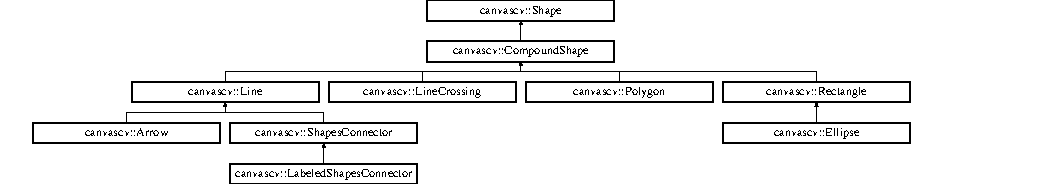
\includegraphics[height=2.466960cm]{classcanvascv_1_1CompoundShape}
\end{center}
\end{figure}
\subsection*{Public Member Functions}
\begin{DoxyCompactItemize}
\item 
virtual void \hyperlink{classcanvascv_1_1CompoundShape_a5b01540c58f0bb5d5a7feccfa38568f9}{set\+Outline\+Color} (const cv\+::\+Scalar \&value)\hypertarget{classcanvascv_1_1CompoundShape_a5b01540c58f0bb5d5a7feccfa38568f9}{}\label{classcanvascv_1_1CompoundShape_a5b01540c58f0bb5d5a7feccfa38568f9}

\begin{DoxyCompactList}\small\item\em set the outline color \end{DoxyCompactList}\item 
virtual void \hyperlink{classcanvascv_1_1CompoundShape_a1c9636ecf2f90a1c532bc8d117f23e79}{set\+Fill\+Color} (const cv\+::\+Scalar \&value)\hypertarget{classcanvascv_1_1CompoundShape_a1c9636ecf2f90a1c532bc8d117f23e79}{}\label{classcanvascv_1_1CompoundShape_a1c9636ecf2f90a1c532bc8d117f23e79}

\begin{DoxyCompactList}\small\item\em set the fill color (fill color is not very useful for shapes right now) \end{DoxyCompactList}\item 
virtual void \hyperlink{classcanvascv_1_1CompoundShape_ac47908d0fb7feb0cb76c4dfa1a3330df}{set\+Thickness} (int value)\hypertarget{classcanvascv_1_1CompoundShape_ac47908d0fb7feb0cb76c4dfa1a3330df}{}\label{classcanvascv_1_1CompoundShape_ac47908d0fb7feb0cb76c4dfa1a3330df}

\begin{DoxyCompactList}\small\item\em set line thickness to use when drawing \end{DoxyCompactList}\item 
virtual void \hyperlink{classcanvascv_1_1CompoundShape_afd64826624ed73c2a5a2ea49ae732b90}{set\+Line\+Type} (int value)\hypertarget{classcanvascv_1_1CompoundShape_afd64826624ed73c2a5a2ea49ae732b90}{}\label{classcanvascv_1_1CompoundShape_afd64826624ed73c2a5a2ea49ae732b90}

\begin{DoxyCompactList}\small\item\em set the line type (L\+I\+N\+E\+\_\+4, L\+I\+N\+E\+\_\+8, L\+I\+N\+E\+\_\+\+AA) \end{DoxyCompactList}\item 
virtual void \hyperlink{classcanvascv_1_1CompoundShape_ab3e29fabe368bd14343e9f7066fbc605}{set\+Locked} (bool value)\hypertarget{classcanvascv_1_1CompoundShape_ab3e29fabe368bd14343e9f7066fbc605}{}\label{classcanvascv_1_1CompoundShape_ab3e29fabe368bd14343e9f7066fbc605}

\begin{DoxyCompactList}\small\item\em set the shape lock state (can/can\textquotesingle{}t be moved/edited) \end{DoxyCompactList}\item 
virtual void \hyperlink{classcanvascv_1_1CompoundShape_a85f3aa483aa21bae7dc60de118a60580}{set\+Visible} (bool value)\hypertarget{classcanvascv_1_1CompoundShape_a85f3aa483aa21bae7dc60de118a60580}{}\label{classcanvascv_1_1CompoundShape_a85f3aa483aa21bae7dc60de118a60580}

\begin{DoxyCompactList}\small\item\em set the shape visible state \end{DoxyCompactList}\item 
virtual std\+::shared\+\_\+ptr$<$ \hyperlink{classcanvascv_1_1Shape}{Shape} $>$ \hyperlink{classcanvascv_1_1CompoundShape_aa9ef6ed91e5a2b6fbd3efe13fbd8e561}{get\+Shape} (int id)
\begin{DoxyCompactList}\small\item\em get\+Shape \end{DoxyCompactList}\end{DoxyCompactItemize}
\subsection*{Protected Member Functions}
\begin{DoxyCompactItemize}
\item 
virtual void \hyperlink{classcanvascv_1_1CompoundShape_a6ec60ee0340ed25274e3ac1349345953}{draw} (cv\+::\+Mat \&canvas)
\begin{DoxyCompactList}\small\item\em draw shape on the canvas \end{DoxyCompactList}\item 
virtual bool \hyperlink{classcanvascv_1_1CompoundShape_a821d046dceaba47114385d1c87e197ce}{mouse\+Pressed} (const cv\+::\+Point \&pos, bool on\+Create=false)
\begin{DoxyCompactList}\small\item\em mouse\+Pressed \end{DoxyCompactList}\item 
virtual bool \hyperlink{classcanvascv_1_1CompoundShape_a387d1705b99d2053306ffd8d8e67b63b}{mouse\+Moved} (const cv\+::\+Point \&pos)
\begin{DoxyCompactList}\small\item\em mouse\+Moved \end{DoxyCompactList}\item 
virtual bool \hyperlink{classcanvascv_1_1CompoundShape_a01cf027fd5f7ec96525949d0c8ae08a1}{mouse\+Released} (const cv\+::\+Point \&pos)
\begin{DoxyCompactList}\small\item\em mouse\+Released \end{DoxyCompactList}\item 
virtual bool \hyperlink{classcanvascv_1_1CompoundShape_ac739f68737099c6f5c6d2c70196cd07b}{key\+Pressed} (int \&key)
\begin{DoxyCompactList}\small\item\em key\+Pressed will be called by \hyperlink{classcanvascv_1_1Canvas}{Canvas} for active shapes \end{DoxyCompactList}\item 
virtual void \hyperlink{classcanvascv_1_1CompoundShape_a4a448d90183494b264d7f673f3c613b4}{lost\+Focus} ()\hypertarget{classcanvascv_1_1CompoundShape_a4a448d90183494b264d7f673f3c613b4}{}\label{classcanvascv_1_1CompoundShape_a4a448d90183494b264d7f673f3c613b4}

\begin{DoxyCompactList}\small\item\em lost\+Focus is called by \hyperlink{classcanvascv_1_1Canvas}{Canvas} if we\textquotesingle{}re in it and just became non-\/active \end{DoxyCompactList}\end{DoxyCompactItemize}
\subsection*{Additional Inherited Members}


\subsection{Detailed Description}
A utility class used by shapes which are the combination of other shapes 

\subsection{Member Function Documentation}
\index{canvascv\+::\+Compound\+Shape@{canvascv\+::\+Compound\+Shape}!draw@{draw}}
\index{draw@{draw}!canvascv\+::\+Compound\+Shape@{canvascv\+::\+Compound\+Shape}}
\subsubsection[{\texorpdfstring{draw(cv\+::\+Mat \&canvas)}{draw(cv::Mat &canvas)}}]{\setlength{\rightskip}{0pt plus 5cm}virtual void canvascv\+::\+Compound\+Shape\+::draw (
\begin{DoxyParamCaption}
\item[{cv\+::\+Mat \&}]{canvas}
\end{DoxyParamCaption}
)\hspace{0.3cm}{\ttfamily [protected]}, {\ttfamily [virtual]}}\hypertarget{classcanvascv_1_1CompoundShape_a6ec60ee0340ed25274e3ac1349345953}{}\label{classcanvascv_1_1CompoundShape_a6ec60ee0340ed25274e3ac1349345953}

\begin{DoxyParams}{Parameters}
{\em canvas} & \\
\hline
\end{DoxyParams}


Implements \hyperlink{classcanvascv_1_1Shape_ab064fdb03d0d94ce84bde0b76b9e62c0}{canvascv\+::\+Shape}.



Reimplemented in \hyperlink{classcanvascv_1_1Line_aad801107019337b6e369fed331539d56}{canvascv\+::\+Line}, \hyperlink{classcanvascv_1_1LineCrossing_a04d251f0cda9f4f51d98d483264fb2dd}{canvascv\+::\+Line\+Crossing}, \hyperlink{classcanvascv_1_1Polygon_a32e073cb9579fdf4645daf14e5143f22}{canvascv\+::\+Polygon}, \hyperlink{classcanvascv_1_1Rectangle_a6b75f528a26e50c35ef9adead3489fc8}{canvascv\+::\+Rectangle}, and \hyperlink{classcanvascv_1_1Arrow_a8ba5b890df49a2d8fc6630df5fe80351}{canvascv\+::\+Arrow}.

\index{canvascv\+::\+Compound\+Shape@{canvascv\+::\+Compound\+Shape}!get\+Shape@{get\+Shape}}
\index{get\+Shape@{get\+Shape}!canvascv\+::\+Compound\+Shape@{canvascv\+::\+Compound\+Shape}}
\subsubsection[{\texorpdfstring{get\+Shape(int id)}{getShape(int id)}}]{\setlength{\rightskip}{0pt plus 5cm}virtual std\+::shared\+\_\+ptr$<${\bf Shape}$>$ canvascv\+::\+Compound\+Shape\+::get\+Shape (
\begin{DoxyParamCaption}
\item[{int}]{id}
\end{DoxyParamCaption}
)\hspace{0.3cm}{\ttfamily [virtual]}}\hypertarget{classcanvascv_1_1CompoundShape_aa9ef6ed91e5a2b6fbd3efe13fbd8e561}{}\label{classcanvascv_1_1CompoundShape_aa9ef6ed91e5a2b6fbd3efe13fbd8e561}
Get internal shapes, which \hyperlink{classcanvascv_1_1Canvas}{Canvas} doesn\textquotesingle{}t know of. 
\begin{DoxyParams}{Parameters}
{\em id} & \\
\hline
\end{DoxyParams}
\begin{DoxyReturn}{Returns}
internal sub shape with requested id 
\end{DoxyReturn}


Reimplemented from \hyperlink{classcanvascv_1_1Shape_a89e585b5a1099f5ce291ded14db7181d}{canvascv\+::\+Shape}.

\index{canvascv\+::\+Compound\+Shape@{canvascv\+::\+Compound\+Shape}!key\+Pressed@{key\+Pressed}}
\index{key\+Pressed@{key\+Pressed}!canvascv\+::\+Compound\+Shape@{canvascv\+::\+Compound\+Shape}}
\subsubsection[{\texorpdfstring{key\+Pressed(int \&key)}{keyPressed(int &key)}}]{\setlength{\rightskip}{0pt plus 5cm}virtual bool canvascv\+::\+Compound\+Shape\+::key\+Pressed (
\begin{DoxyParamCaption}
\item[{int \&}]{key}
\end{DoxyParamCaption}
)\hspace{0.3cm}{\ttfamily [protected]}, {\ttfamily [virtual]}}\hypertarget{classcanvascv_1_1CompoundShape_ac739f68737099c6f5c6d2c70196cd07b}{}\label{classcanvascv_1_1CompoundShape_ac739f68737099c6f5c6d2c70196cd07b}

\begin{DoxyParams}{Parameters}
{\em key} & was pressed. You must set it to -\/1 if you consumed it. \\
\hline
\end{DoxyParams}
\begin{DoxyReturn}{Returns}
true if we want to stay in focus and false otherwise 
\end{DoxyReturn}


Reimplemented from \hyperlink{classcanvascv_1_1Shape_a7419dc43b9be99010e2b3bb973efbd37}{canvascv\+::\+Shape}.



Reimplemented in \hyperlink{classcanvascv_1_1Line_a4059736cde05ffc90dda8ed1ff4f9ba2}{canvascv\+::\+Line}, \hyperlink{classcanvascv_1_1Polygon_aca22b914de1ced559faf4fd5426073ff}{canvascv\+::\+Polygon}, and \hyperlink{classcanvascv_1_1Rectangle_a905ec50de408cbc2df0158bafff210d1}{canvascv\+::\+Rectangle}.

\index{canvascv\+::\+Compound\+Shape@{canvascv\+::\+Compound\+Shape}!mouse\+Moved@{mouse\+Moved}}
\index{mouse\+Moved@{mouse\+Moved}!canvascv\+::\+Compound\+Shape@{canvascv\+::\+Compound\+Shape}}
\subsubsection[{\texorpdfstring{mouse\+Moved(const cv\+::\+Point \&pos)}{mouseMoved(const cv::Point &pos)}}]{\setlength{\rightskip}{0pt plus 5cm}virtual bool canvascv\+::\+Compound\+Shape\+::mouse\+Moved (
\begin{DoxyParamCaption}
\item[{const cv\+::\+Point \&}]{pos}
\end{DoxyParamCaption}
)\hspace{0.3cm}{\ttfamily [protected]}, {\ttfamily [virtual]}}\hypertarget{classcanvascv_1_1CompoundShape_a387d1705b99d2053306ffd8d8e67b63b}{}\label{classcanvascv_1_1CompoundShape_a387d1705b99d2053306ffd8d8e67b63b}

\begin{DoxyEnumerate}
\item Was a mouse moved over this shape?
\item If shape is during edit, then these are the mouse position. 
\begin{DoxyParams}{Parameters}
{\em pos} & \\
\hline
\end{DoxyParams}
\begin{DoxyReturn}{Returns}
true if a mouse moved over this shape, or it is during edit. false otherwise. 
\end{DoxyReturn}

\end{DoxyEnumerate}

Implements \hyperlink{classcanvascv_1_1Shape_acc72c3f645927c135dbc589e2c8678d4}{canvascv\+::\+Shape}.



Reimplemented in \hyperlink{classcanvascv_1_1Line_ad758464d98d455d2ea3aa591667fb595}{canvascv\+::\+Line}, \hyperlink{classcanvascv_1_1Polygon_aacc442ef4c0438ddb78c6ccce8e86618}{canvascv\+::\+Polygon}, and \hyperlink{classcanvascv_1_1Rectangle_a0e363f915b93526e034dbfd5550597db}{canvascv\+::\+Rectangle}.

\index{canvascv\+::\+Compound\+Shape@{canvascv\+::\+Compound\+Shape}!mouse\+Pressed@{mouse\+Pressed}}
\index{mouse\+Pressed@{mouse\+Pressed}!canvascv\+::\+Compound\+Shape@{canvascv\+::\+Compound\+Shape}}
\subsubsection[{\texorpdfstring{mouse\+Pressed(const cv\+::\+Point \&pos, bool on\+Create=false)}{mousePressed(const cv::Point &pos, bool onCreate=false)}}]{\setlength{\rightskip}{0pt plus 5cm}virtual bool canvascv\+::\+Compound\+Shape\+::mouse\+Pressed (
\begin{DoxyParamCaption}
\item[{const cv\+::\+Point \&}]{pos, }
\item[{bool}]{on\+Create = {\ttfamily false}}
\end{DoxyParamCaption}
)\hspace{0.3cm}{\ttfamily [protected]}, {\ttfamily [virtual]}}\hypertarget{classcanvascv_1_1CompoundShape_a821d046dceaba47114385d1c87e197ce}{}\label{classcanvascv_1_1CompoundShape_a821d046dceaba47114385d1c87e197ce}

\begin{DoxyParams}{Parameters}
{\em pos} & \\
\hline
{\em on\+Create} & is true if this is the mouse press which cerated this shape \\
\hline
\end{DoxyParams}
\begin{DoxyReturn}{Returns}
true for keep in focus, false for leave focus 
\end{DoxyReturn}


Implements \hyperlink{classcanvascv_1_1Shape_aa332adef968829dd7744cb1f6a491879}{canvascv\+::\+Shape}.



Reimplemented in \hyperlink{classcanvascv_1_1Line_aab4d23d336fe71c6d7000d8da9a54269}{canvascv\+::\+Line}, \hyperlink{classcanvascv_1_1LineCrossing_a8232b4101d5533b12129c4d145ffc54d}{canvascv\+::\+Line\+Crossing}, \hyperlink{classcanvascv_1_1ShapesConnector_a6c6400403c6c2809af1e0a64e477f592}{canvascv\+::\+Shapes\+Connector}, \hyperlink{classcanvascv_1_1Polygon_a87ce20dbc22fd0ce39d6e81de5e515ae}{canvascv\+::\+Polygon}, and \hyperlink{classcanvascv_1_1Rectangle_ac39753497259e3f6a7fdac667cd08596}{canvascv\+::\+Rectangle}.

\index{canvascv\+::\+Compound\+Shape@{canvascv\+::\+Compound\+Shape}!mouse\+Released@{mouse\+Released}}
\index{mouse\+Released@{mouse\+Released}!canvascv\+::\+Compound\+Shape@{canvascv\+::\+Compound\+Shape}}
\subsubsection[{\texorpdfstring{mouse\+Released(const cv\+::\+Point \&pos)}{mouseReleased(const cv::Point &pos)}}]{\setlength{\rightskip}{0pt plus 5cm}virtual bool canvascv\+::\+Compound\+Shape\+::mouse\+Released (
\begin{DoxyParamCaption}
\item[{const cv\+::\+Point \&}]{pos}
\end{DoxyParamCaption}
)\hspace{0.3cm}{\ttfamily [protected]}, {\ttfamily [virtual]}}\hypertarget{classcanvascv_1_1CompoundShape_a01cf027fd5f7ec96525949d0c8ae08a1}{}\label{classcanvascv_1_1CompoundShape_a01cf027fd5f7ec96525949d0c8ae08a1}

\begin{DoxyParams}{Parameters}
{\em pos} & \\
\hline
\end{DoxyParams}
\begin{DoxyReturn}{Returns}
true for keep in focus, false for leave focus 
\end{DoxyReturn}


Implements \hyperlink{classcanvascv_1_1Shape_a8cbe386ff880c9830c0e4a97b335abf0}{canvascv\+::\+Shape}.



Reimplemented in \hyperlink{classcanvascv_1_1Line_ace7269cabd2acbb2c9da009740f46fa3}{canvascv\+::\+Line}, \hyperlink{classcanvascv_1_1ShapesConnector_a56ab827f3d72e495ccfd1101807413f8}{canvascv\+::\+Shapes\+Connector}, \hyperlink{classcanvascv_1_1Polygon_afea6bbe1beef916e6ec47ed257cb2374}{canvascv\+::\+Polygon}, and \hyperlink{classcanvascv_1_1Rectangle_a6a54774d57d88d053cfb8d5a41878b16}{canvascv\+::\+Rectangle}.



The documentation for this class was generated from the following file\+:\begin{DoxyCompactItemize}
\item 
Canvas\+C\+V-\/doxygen/src/canvascv/shapes/compoundshape.\+h\end{DoxyCompactItemize}

\hypertarget{classcanvascv_1_1CompoundWidget}{}\section{canvascv\+:\+:Compound\+Widget Class Reference}
\label{classcanvascv_1_1CompoundWidget}\index{canvascv\+::\+Compound\+Widget@{canvascv\+::\+Compound\+Widget}}


The \hyperlink{classcanvascv_1_1CompoundWidget}{Compound\+Widget} class.  




{\ttfamily \#include $<$compoundwidget.\+h$>$}

Inheritance diagram for canvascv\+:\+:Compound\+Widget\+:\begin{figure}[H]
\begin{center}
\leavevmode
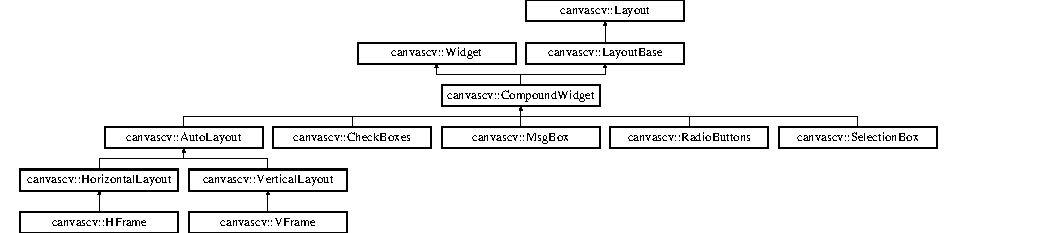
\includegraphics[height=3.128491cm]{classcanvascv_1_1CompoundWidget}
\end{center}
\end{figure}
\subsection*{Public Member Functions}
\begin{DoxyCompactItemize}
\item 
virtual void \hyperlink{classcanvascv_1_1CompoundWidget_a89acccaf003b00ec8310484e321d74a0}{set\+Outline\+Color} (const cv\+::\+Scalar \&value)\hypertarget{classcanvascv_1_1CompoundWidget_a89acccaf003b00ec8310484e321d74a0}{}\label{classcanvascv_1_1CompoundWidget_a89acccaf003b00ec8310484e321d74a0}

\begin{DoxyCompactList}\small\item\em delegate to internal \hyperlink{classcanvascv_1_1Widget}{Widget} parts added by derived classes \end{DoxyCompactList}\item 
virtual void \hyperlink{classcanvascv_1_1CompoundWidget_ae5b81096c6436130475e977e894257d9}{set\+Fill\+Color} (const cv\+::\+Scalar \&value)\hypertarget{classcanvascv_1_1CompoundWidget_ae5b81096c6436130475e977e894257d9}{}\label{classcanvascv_1_1CompoundWidget_ae5b81096c6436130475e977e894257d9}

\begin{DoxyCompactList}\small\item\em delegate to internal \hyperlink{classcanvascv_1_1Widget}{Widget} parts added by derived classes \end{DoxyCompactList}\item 
virtual void \hyperlink{classcanvascv_1_1CompoundWidget_a59188d0a0a947dab227b2b26263e8698}{set\+Select\+Color} (const cv\+::\+Scalar \&value)\hypertarget{classcanvascv_1_1CompoundWidget_a59188d0a0a947dab227b2b26263e8698}{}\label{classcanvascv_1_1CompoundWidget_a59188d0a0a947dab227b2b26263e8698}

\begin{DoxyCompactList}\small\item\em delegate to internal \hyperlink{classcanvascv_1_1Widget}{Widget} parts added by derived classes \end{DoxyCompactList}\item 
virtual void \hyperlink{classcanvascv_1_1CompoundWidget_abc8be92c3042fe25004c0638b64251b6}{set\+Thickness} (int value)\hypertarget{classcanvascv_1_1CompoundWidget_abc8be92c3042fe25004c0638b64251b6}{}\label{classcanvascv_1_1CompoundWidget_abc8be92c3042fe25004c0638b64251b6}

\begin{DoxyCompactList}\small\item\em delegate to internal \hyperlink{classcanvascv_1_1Widget}{Widget} parts added by derived classes \end{DoxyCompactList}\item 
virtual void \hyperlink{classcanvascv_1_1CompoundWidget_ac45ea9109d6b73c65b6a631dbc9595c5}{set\+Line\+Type} (int value)\hypertarget{classcanvascv_1_1CompoundWidget_ac45ea9109d6b73c65b6a631dbc9595c5}{}\label{classcanvascv_1_1CompoundWidget_ac45ea9109d6b73c65b6a631dbc9595c5}

\begin{DoxyCompactList}\small\item\em delegate to internal \hyperlink{classcanvascv_1_1Widget}{Widget} parts added by derived classes \end{DoxyCompactList}\item 
virtual void \hyperlink{classcanvascv_1_1CompoundWidget_ab81cd287c73d8ed098d0914596dd40ba}{set\+Visible} (bool value)\hypertarget{classcanvascv_1_1CompoundWidget_ab81cd287c73d8ed098d0914596dd40ba}{}\label{classcanvascv_1_1CompoundWidget_ab81cd287c73d8ed098d0914596dd40ba}

\begin{DoxyCompactList}\small\item\em delegate to internal \hyperlink{classcanvascv_1_1Widget}{Widget} parts added by derived classes \end{DoxyCompactList}\item 
virtual const std\+::string \& \hyperlink{classcanvascv_1_1CompoundWidget_a7b8afb0ea8e8803f201b9ee8aa7e153a}{get\+Status\+Msg} () const \hypertarget{classcanvascv_1_1CompoundWidget_a7b8afb0ea8e8803f201b9ee8aa7e153a}{}\label{classcanvascv_1_1CompoundWidget_a7b8afb0ea8e8803f201b9ee8aa7e153a}

\begin{DoxyCompactList}\small\item\em delegate to active widget or to our derived class if none active \end{DoxyCompactList}\item 
virtual void \hyperlink{classcanvascv_1_1CompoundWidget_a28d73640776bc428f008a9b14facd3f9}{translate} (const cv\+::\+Point \&translation)\hypertarget{classcanvascv_1_1CompoundWidget_a28d73640776bc428f008a9b14facd3f9}{}\label{classcanvascv_1_1CompoundWidget_a28d73640776bc428f008a9b14facd3f9}

\begin{DoxyCompactList}\small\item\em delegate to internal \hyperlink{classcanvascv_1_1Widget}{Widget} parts added by derived classes \end{DoxyCompactList}\item 
void \hyperlink{classcanvascv_1_1CompoundWidget_aa7d0f488468fca5707aa49ea35e9c67e}{do\+For\+All} (\hyperlink{classcanvascv_1_1Widget_ad27bca771ee1c14454c77c91d9d49925}{C\+B\+Widget} cb, int recurse\+Level, bool do\+On\+Self)
\begin{DoxyCompactList}\small\item\em do\+For\+All \end{DoxyCompactList}\item 
virtual const cv\+::\+Rect \& \hyperlink{classcanvascv_1_1CompoundWidget_a5dd95e74613437ed56821b8ae796d64f}{get\+Rect} ()\hypertarget{classcanvascv_1_1CompoundWidget_a5dd95e74613437ed56821b8ae796d64f}{}\label{classcanvascv_1_1CompoundWidget_a5dd95e74613437ed56821b8ae796d64f}

\begin{DoxyCompactList}\small\item\em Actual size the widget is occupying due to \hyperlink{classcanvascv_1_1Layout}{Layout} manager. \end{DoxyCompactList}\end{DoxyCompactItemize}
\subsection*{Protected Member Functions}
\begin{DoxyCompactItemize}
\item 
virtual void \hyperlink{classcanvascv_1_1CompoundWidget_aac9694f4fbc3e31d3b5d37df4a25a753}{recalc} () final\hypertarget{classcanvascv_1_1CompoundWidget_aac9694f4fbc3e31d3b5d37df4a25a753}{}\label{classcanvascv_1_1CompoundWidget_aac9694f4fbc3e31d3b5d37df4a25a753}

\begin{DoxyCompactList}\small\item\em delegate to internal \hyperlink{classcanvascv_1_1Widget}{Widget} parts added by derived classes \end{DoxyCompactList}\item 
virtual void \hyperlink{classcanvascv_1_1CompoundWidget_a4a4f8241d6fd187ffcae2c7968f13864}{recalc\+Compound} ()=0
\begin{DoxyCompactList}\small\item\em recalc\+Compound \end{DoxyCompactList}\item 
virtual void \hyperlink{classcanvascv_1_1CompoundWidget_aea537ebb4b6988a052dea60c1ab7772e}{add\+Widget} (const std\+::shared\+\_\+ptr$<$ \hyperlink{classcanvascv_1_1Widget}{Widget} $>$ \&widget)\hypertarget{classcanvascv_1_1CompoundWidget_aea537ebb4b6988a052dea60c1ab7772e}{}\label{classcanvascv_1_1CompoundWidget_aea537ebb4b6988a052dea60c1ab7772e}

\begin{DoxyCompactList}\small\item\em adds the widget to this \hyperlink{classcanvascv_1_1Layout}{Layout} after removing it from it\textquotesingle{}s previous layout \end{DoxyCompactList}\item 
virtual std\+::shared\+\_\+ptr$<$ \hyperlink{classcanvascv_1_1Widget}{Widget} $>$ \hyperlink{classcanvascv_1_1CompoundWidget_ad4a37bf31f9cf6410b41526a5b83c75a}{rmv\+Widget} (const std\+::shared\+\_\+ptr$<$ \hyperlink{classcanvascv_1_1Widget}{Widget} $>$ \&widget)
\begin{DoxyCompactList}\small\item\em rmv\+Widget \end{DoxyCompactList}\item 
virtual void \hyperlink{classcanvascv_1_1CompoundWidget_a1ceebdcae41eadc0796306ca88698411}{render\+On} (cv\+::\+Mat \&dst)
\begin{DoxyCompactList}\small\item\em render the widget to dst \end{DoxyCompactList}\item 
virtual void \hyperlink{classcanvascv_1_1CompoundWidget_a2cabb8158780247ddc9f2b7bc3db49ca}{draw\+FG} (cv\+::\+Mat \&dst)\hypertarget{classcanvascv_1_1CompoundWidget_a2cabb8158780247ddc9f2b7bc3db49ca}{}\label{classcanvascv_1_1CompoundWidget_a2cabb8158780247ddc9f2b7bc3db49ca}

\begin{DoxyCompactList}\small\item\em dst is the roi of the widget size and not the full image \end{DoxyCompactList}\item 
virtual bool \hyperlink{classcanvascv_1_1CompoundWidget_a00a67f3864155e74c60df66bc78c940e}{is\+At\+Pos} (const cv\+::\+Point \&pos)
\begin{DoxyCompactList}\small\item\em is\+At\+Pos \end{DoxyCompactList}\item 
virtual const cv\+::\+Rect \& \hyperlink{classcanvascv_1_1CompoundWidget_aa28f3ee799cc30222f0f272ea070ee30}{get\+Minimal\+Rect} ()\hypertarget{classcanvascv_1_1CompoundWidget_aa28f3ee799cc30222f0f272ea070ee30}{}\label{classcanvascv_1_1CompoundWidget_aa28f3ee799cc30222f0f272ea070ee30}

\begin{DoxyCompactList}\small\item\em Minimal size the widget coould have occupy. \end{DoxyCompactList}\end{DoxyCompactItemize}
\subsection*{Additional Inherited Members}


\subsection{Detailed Description}
Utility class to help easy creation of complex widgets and \hyperlink{classcanvascv_1_1Layout}{Layout} managers. \begin{Desc}
\item[Examples\+: ]\par
\hyperlink{example_add_widget_8cpp-example}{example\+\_\+add\+\_\+widget.\+cpp}.\end{Desc}


\subsection{Member Function Documentation}
\index{canvascv\+::\+Compound\+Widget@{canvascv\+::\+Compound\+Widget}!do\+For\+All@{do\+For\+All}}
\index{do\+For\+All@{do\+For\+All}!canvascv\+::\+Compound\+Widget@{canvascv\+::\+Compound\+Widget}}
\subsubsection[{\texorpdfstring{do\+For\+All(\+C\+B\+Widget cb, int recurse\+Level, bool do\+On\+Self)}{doForAll(CBWidget cb, int recurseLevel, bool doOnSelf)}}]{\setlength{\rightskip}{0pt plus 5cm}void canvascv\+::\+Compound\+Widget\+::do\+For\+All (
\begin{DoxyParamCaption}
\item[{{\bf C\+B\+Widget}}]{cb, }
\item[{int}]{recurse\+Level, }
\item[{bool}]{do\+On\+Self}
\end{DoxyParamCaption}
)}\hypertarget{classcanvascv_1_1CompoundWidget_aa7d0f488468fca5707aa49ea35e9c67e}{}\label{classcanvascv_1_1CompoundWidget_aa7d0f488468fca5707aa49ea35e9c67e}
invoke the cb for all included widgets. This is usually not necessary since the above methods delegate to both contained widgets and self. 
\begin{DoxyParams}{Parameters}
{\em cb} & is what to execute on widgets \\
\hline
{\em recurse\+Level} & is how deep to go when updating kids\+:
\begin{DoxyItemize}
\item -\/1 means all decendents at all levels
\item 0 means only current level (do\+On\+Self needs to be also \textquotesingle{}true\textquotesingle{})
\item n$>$0 means up to kids at level n (1 is children, 2 is also grandchildren, etc.) 
\end{DoxyItemize}\\
\hline
{\em do\+On\+Self} & is if to also invoke the cb on the first parent \\
\hline
\end{DoxyParams}
\index{canvascv\+::\+Compound\+Widget@{canvascv\+::\+Compound\+Widget}!is\+At\+Pos@{is\+At\+Pos}}
\index{is\+At\+Pos@{is\+At\+Pos}!canvascv\+::\+Compound\+Widget@{canvascv\+::\+Compound\+Widget}}
\subsubsection[{\texorpdfstring{is\+At\+Pos(const cv\+::\+Point \&pos)}{isAtPos(const cv::Point &pos)}}]{\setlength{\rightskip}{0pt plus 5cm}virtual bool canvascv\+::\+Compound\+Widget\+::is\+At\+Pos (
\begin{DoxyParamCaption}
\item[{const cv\+::\+Point \&}]{pos}
\end{DoxyParamCaption}
)\hspace{0.3cm}{\ttfamily [protected]}, {\ttfamily [virtual]}}\hypertarget{classcanvascv_1_1CompoundWidget_a00a67f3864155e74c60df66bc78c940e}{}\label{classcanvascv_1_1CompoundWidget_a00a67f3864155e74c60df66bc78c940e}

\begin{DoxyParams}{Parameters}
{\em pos} & \\
\hline
\end{DoxyParams}
\begin{DoxyReturn}{Returns}
true or false if at location 
\end{DoxyReturn}


Reimplemented from \hyperlink{classcanvascv_1_1Widget_a3ea1ca9e064178a5647ce04bc531655f}{canvascv\+::\+Widget}.

\index{canvascv\+::\+Compound\+Widget@{canvascv\+::\+Compound\+Widget}!recalc\+Compound@{recalc\+Compound}}
\index{recalc\+Compound@{recalc\+Compound}!canvascv\+::\+Compound\+Widget@{canvascv\+::\+Compound\+Widget}}
\subsubsection[{\texorpdfstring{recalc\+Compound()=0}{recalcCompound()=0}}]{\setlength{\rightskip}{0pt plus 5cm}virtual void canvascv\+::\+Compound\+Widget\+::recalc\+Compound (
\begin{DoxyParamCaption}
{}
\end{DoxyParamCaption}
)\hspace{0.3cm}{\ttfamily [protected]}, {\ttfamily [pure virtual]}}\hypertarget{classcanvascv_1_1CompoundWidget_a4a4f8241d6fd187ffcae2c7968f13864}{}\label{classcanvascv_1_1CompoundWidget_a4a4f8241d6fd187ffcae2c7968f13864}
Your BG size recalculation/allocation and FG drawing is done here. It is done semi automatically. Is you invoke setters in this method on your internal widgets, then make sure to update them and/or their layout 

Implemented in \hyperlink{classcanvascv_1_1MsgBox_a1eea452acb76e5a5a0588bf83cc91325}{canvascv\+::\+Msg\+Box}, \hyperlink{classcanvascv_1_1CheckBoxes_a50cae1ae73c9d69f864bc7fe6d6fedd6}{canvascv\+::\+Check\+Boxes}, \hyperlink{classcanvascv_1_1RadioButtons_af4f863f492ca723a0ddac03139a1f187}{canvascv\+::\+Radio\+Buttons}, \hyperlink{classcanvascv_1_1SelectionBox_a78bf141cda79618e972f173627d07e1a}{canvascv\+::\+Selection\+Box}, \hyperlink{classcanvascv_1_1VerticalLayout_a0d4661776d5cb6dc4eccebcb3e5ff17c}{canvascv\+::\+Vertical\+Layout}, and \hyperlink{classcanvascv_1_1HorizontalLayout_ab6e59f3499bde32be889d3898cdf6888}{canvascv\+::\+Horizontal\+Layout}.

\index{canvascv\+::\+Compound\+Widget@{canvascv\+::\+Compound\+Widget}!render\+On@{render\+On}}
\index{render\+On@{render\+On}!canvascv\+::\+Compound\+Widget@{canvascv\+::\+Compound\+Widget}}
\subsubsection[{\texorpdfstring{render\+On(cv\+::\+Mat \&dst)}{renderOn(cv::Mat &dst)}}]{\setlength{\rightskip}{0pt plus 5cm}virtual void canvascv\+::\+Compound\+Widget\+::render\+On (
\begin{DoxyParamCaption}
\item[{cv\+::\+Mat \&}]{dst}
\end{DoxyParamCaption}
)\hspace{0.3cm}{\ttfamily [protected]}, {\ttfamily [virtual]}}\hypertarget{classcanvascv_1_1CompoundWidget_a1ceebdcae41eadc0796306ca88698411}{}\label{classcanvascv_1_1CompoundWidget_a1ceebdcae41eadc0796306ca88698411}

\begin{DoxyParams}{Parameters}
{\em dst} & is the full size image \\
\hline
\end{DoxyParams}


Reimplemented from \hyperlink{classcanvascv_1_1Widget_a74130cdbcc974dfa7e8ceb9a53c112b9}{canvascv\+::\+Widget}.

\index{canvascv\+::\+Compound\+Widget@{canvascv\+::\+Compound\+Widget}!rmv\+Widget@{rmv\+Widget}}
\index{rmv\+Widget@{rmv\+Widget}!canvascv\+::\+Compound\+Widget@{canvascv\+::\+Compound\+Widget}}
\subsubsection[{\texorpdfstring{rmv\+Widget(const std\+::shared\+\_\+ptr$<$ Widget $>$ \&widget)}{rmvWidget(const std::shared_ptr< Widget > &widget)}}]{\setlength{\rightskip}{0pt plus 5cm}virtual std\+::shared\+\_\+ptr$<${\bf Widget}$>$ canvascv\+::\+Compound\+Widget\+::rmv\+Widget (
\begin{DoxyParamCaption}
\item[{const std\+::shared\+\_\+ptr$<$ {\bf Widget} $>$ \&}]{widget}
\end{DoxyParamCaption}
)\hspace{0.3cm}{\ttfamily [protected]}, {\ttfamily [virtual]}}\hypertarget{classcanvascv_1_1CompoundWidget_ad4a37bf31f9cf6410b41526a5b83c75a}{}\label{classcanvascv_1_1CompoundWidget_ad4a37bf31f9cf6410b41526a5b83c75a}

\begin{DoxyParams}{Parameters}
{\em widget} & will be removed from this \hyperlink{classcanvascv_1_1Layout}{Layout} \\
\hline
\end{DoxyParams}
\begin{DoxyReturn}{Returns}
filled shared\+\_\+ptr to removed widget or empty if not found 
\end{DoxyReturn}
\begin{DoxyNote}{Note}
Widgets must be in layouts to be displayed correctly. 
\end{DoxyNote}


Implements \hyperlink{classcanvascv_1_1Layout_a7b532816232c436ea5b6e7c4c3254779}{canvascv\+::\+Layout}.



Reimplemented in \hyperlink{classcanvascv_1_1AutoLayout_abc436c90f50a5331c391e351bef9e659}{canvascv\+::\+Auto\+Layout}.



The documentation for this class was generated from the following file\+:\begin{DoxyCompactItemize}
\item 
Canvas\+C\+V-\/doxygen/src/canvascv/widgets/compoundwidget.\+h\end{DoxyCompactItemize}

\hypertarget{classcanvascv_1_1Consts}{}\section{canvascv\+:\+:Consts Class Reference}
\label{classcanvascv_1_1Consts}\index{canvascv\+::\+Consts@{canvascv\+::\+Consts}}


The \hyperlink{classcanvascv_1_1Consts}{Consts} class.  




{\ttfamily \#include $<$consts.\+h$>$}



\subsection{Detailed Description}
The place for global constants constants 

The documentation for this class was generated from the following file\+:\begin{DoxyCompactItemize}
\item 
Canvas\+C\+V-\/doxygen/src/canvascv/consts.\+h\end{DoxyCompactItemize}

\hypertarget{classcanvascv_1_1Ellipse}{}\section{canvascv\+:\+:Ellipse Class Reference}
\label{classcanvascv_1_1Ellipse}\index{canvascv\+::\+Ellipse@{canvascv\+::\+Ellipse}}


The \hyperlink{classcanvascv_1_1Ellipse}{Ellipse} class.  




{\ttfamily \#include $<$ellipse.\+h$>$}

Inheritance diagram for canvascv\+:\+:Ellipse\+:\begin{figure}[H]
\begin{center}
\leavevmode
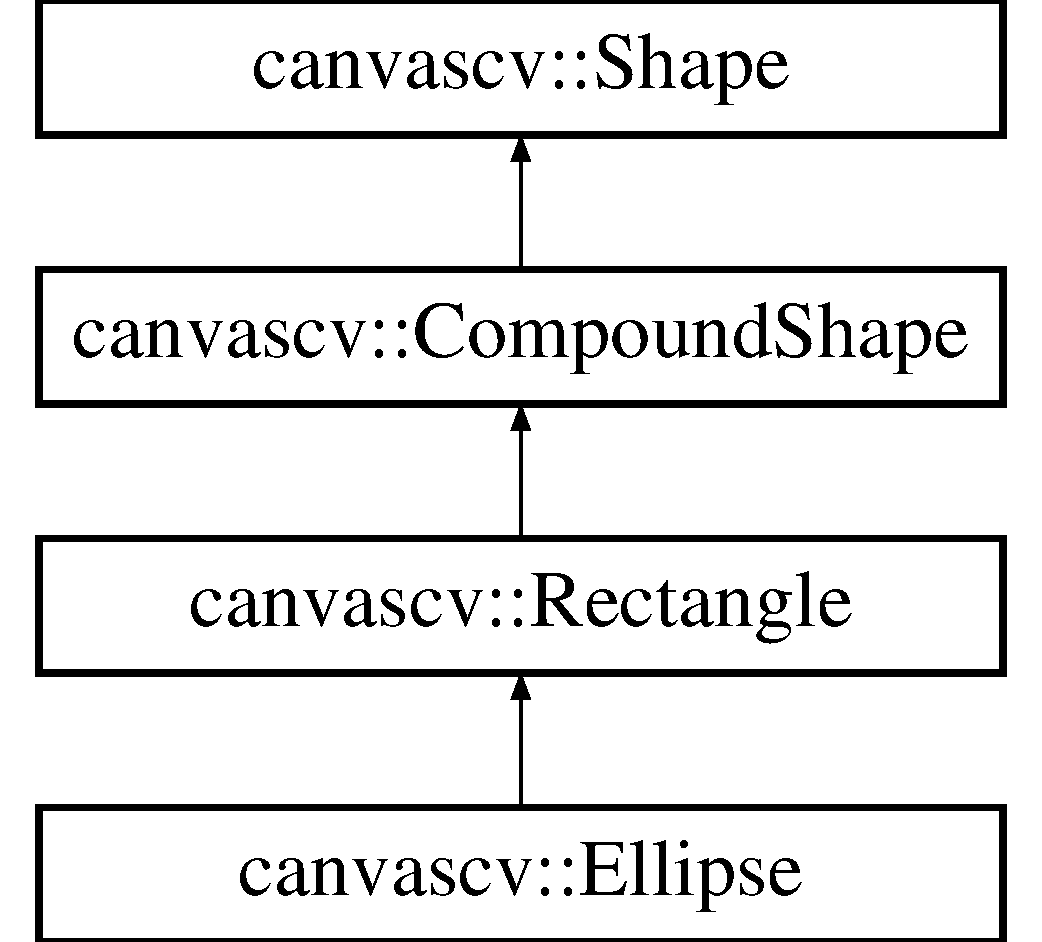
\includegraphics[height=4.000000cm]{classcanvascv_1_1Ellipse}
\end{center}
\end{figure}
\subsection*{Public Member Functions}
\begin{DoxyCompactItemize}
\item 
virtual const char $\ast$ \hyperlink{classcanvascv_1_1Ellipse_a15df73cf790d34b71749ec0e5d6d0331}{get\+Type} () const 
\begin{DoxyCompactList}\small\item\em get\+Type is always implemented by derived to return the same static pointer per shape. \end{DoxyCompactList}\end{DoxyCompactItemize}
\subsection*{Additional Inherited Members}


\subsection{Detailed Description}
Allows you to draw a rotatable ellipse by mouse or from code \begin{Desc}
\item[Examples\+: ]\par
\hyperlink{example_shapes_widgets_8cpp-example}{example\+\_\+shapes\+\_\+widgets.\+cpp}.\end{Desc}


\subsection{Member Function Documentation}
\index{canvascv\+::\+Ellipse@{canvascv\+::\+Ellipse}!get\+Type@{get\+Type}}
\index{get\+Type@{get\+Type}!canvascv\+::\+Ellipse@{canvascv\+::\+Ellipse}}
\subsubsection[{\texorpdfstring{get\+Type() const }{getType() const }}]{\setlength{\rightskip}{0pt plus 5cm}virtual const char$\ast$ canvascv\+::\+Ellipse\+::get\+Type (
\begin{DoxyParamCaption}
{}
\end{DoxyParamCaption}
) const\hspace{0.3cm}{\ttfamily [virtual]}}\hypertarget{classcanvascv_1_1Ellipse_a15df73cf790d34b71749ec0e5d6d0331}{}\label{classcanvascv_1_1Ellipse_a15df73cf790d34b71749ec0e5d6d0331}
\begin{DoxyReturn}{Returns}
const char $\ast$ pointer to string with shape type name 
\end{DoxyReturn}


Reimplemented from \hyperlink{classcanvascv_1_1Rectangle_aa66625e0e783029524f669a3113020f5}{canvascv\+::\+Rectangle}.



The documentation for this class was generated from the following file\+:\begin{DoxyCompactItemize}
\item 
Canvas\+C\+V-\/doxygen/src/canvascv/shapes/ellipse.\+h\end{DoxyCompactItemize}

\hypertarget{classcanvascv_1_1Handle}{}\section{canvascv\+:\+:Handle Class Reference}
\label{classcanvascv_1_1Handle}\index{canvascv\+::\+Handle@{canvascv\+::\+Handle}}


The \hyperlink{classcanvascv_1_1Handle}{Handle} class.  




{\ttfamily \#include $<$handle.\+h$>$}

Inheritance diagram for canvascv\+:\+:Handle\+:\begin{figure}[H]
\begin{center}
\leavevmode
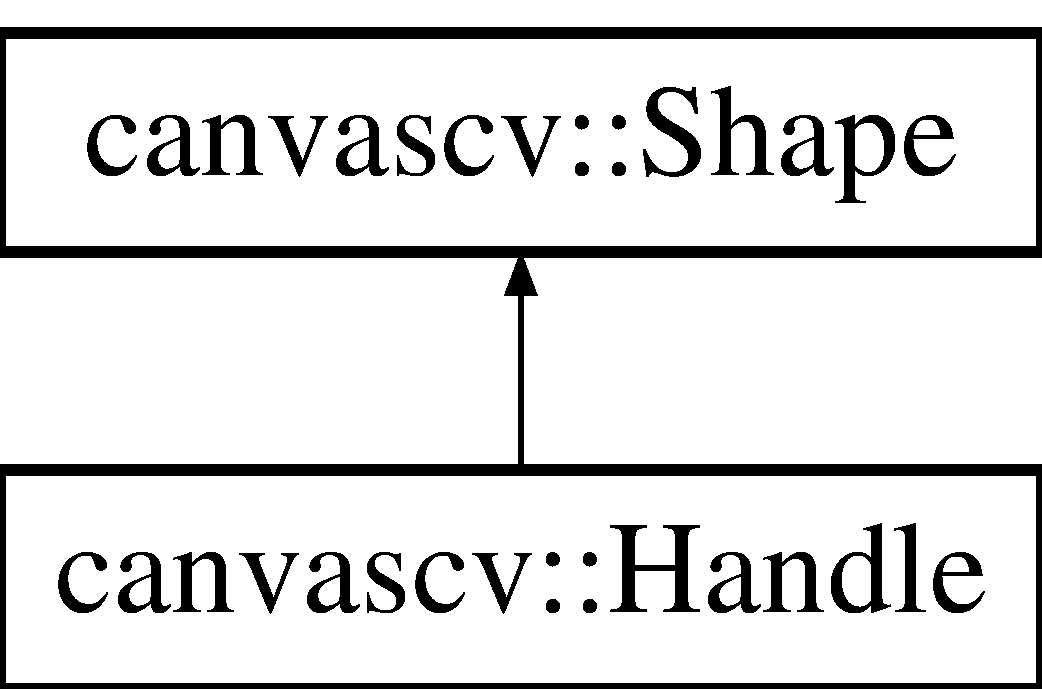
\includegraphics[height=2.000000cm]{classcanvascv_1_1Handle}
\end{center}
\end{figure}
\subsection*{Public Member Functions}
\begin{DoxyCompactItemize}
\item 
const cv\+::\+Point \& \hyperlink{classcanvascv_1_1Handle_af7f37f216c87e0ddb0c3028308a0ac08}{operator()} () const \hypertarget{classcanvascv_1_1Handle_af7f37f216c87e0ddb0c3028308a0ac08}{}\label{classcanvascv_1_1Handle_af7f37f216c87e0ddb0c3028308a0ac08}

\begin{DoxyCompactList}\small\item\em return the Point location of this \hyperlink{classcanvascv_1_1Handle}{Handle} \end{DoxyCompactList}\item 
void \hyperlink{classcanvascv_1_1Handle_a57758e2de29de462f4bda5f7a50b0c96}{set\+Pos} (const cv\+::\+Point \&pos, bool notify=true)
\begin{DoxyCompactList}\small\item\em set\+Pos \end{DoxyCompactList}\item 
int \hyperlink{classcanvascv_1_1Handle_a549813832ba1514040a0bf2c9397f10d}{get\+Radius} () const \hypertarget{classcanvascv_1_1Handle_a549813832ba1514040a0bf2c9397f10d}{}\label{classcanvascv_1_1Handle_a549813832ba1514040a0bf2c9397f10d}

\begin{DoxyCompactList}\small\item\em return the radius of this circled handle \end{DoxyCompactList}\item 
C\+B\+ID \hyperlink{classcanvascv_1_1Handle_adf028dcb7c12a711351d9a5794b1df69}{add\+Pos\+Changed\+CB} (Pos\+Changed\+CB cb)\hypertarget{classcanvascv_1_1Handle_adf028dcb7c12a711351d9a5794b1df69}{}\label{classcanvascv_1_1Handle_adf028dcb7c12a711351d9a5794b1df69}

\begin{DoxyCompactList}\small\item\em register to be notified when this handle changes \end{DoxyCompactList}\item 
void \hyperlink{classcanvascv_1_1Handle_a9d81b805be12d424bc59cbb7f73745ea}{del\+Pos\+Changed\+CB} (const C\+B\+ID \&id)\hypertarget{classcanvascv_1_1Handle_a9d81b805be12d424bc59cbb7f73745ea}{}\label{classcanvascv_1_1Handle_a9d81b805be12d424bc59cbb7f73745ea}

\begin{DoxyCompactList}\small\item\em unregister to be notified when this handle changes \end{DoxyCompactList}\item 
void \hyperlink{classcanvascv_1_1Handle_aca046d84a3e080af8b44a09b4efd6469}{connect} (\hyperlink{classcanvascv_1_1Handle}{Handle} \&other)\hypertarget{classcanvascv_1_1Handle_aca046d84a3e080af8b44a09b4efd6469}{}\label{classcanvascv_1_1Handle_aca046d84a3e080af8b44a09b4efd6469}

\begin{DoxyCompactList}\small\item\em connect to a handle to change when we change \end{DoxyCompactList}\item 
void \hyperlink{classcanvascv_1_1Handle_afa78f039c0544fe98f20a0e40fb2bb45}{disconnect} (\hyperlink{classcanvascv_1_1Handle}{Handle} \&other)\hypertarget{classcanvascv_1_1Handle_afa78f039c0544fe98f20a0e40fb2bb45}{}\label{classcanvascv_1_1Handle_afa78f039c0544fe98f20a0e40fb2bb45}

\begin{DoxyCompactList}\small\item\em disconnect from a handle that needed to change with us \end{DoxyCompactList}\item 
virtual bool \hyperlink{classcanvascv_1_1Handle_a87de6edeed8ca14dbc5c3a7a127fa5a5}{is\+At\+Pos} (const cv\+::\+Point \&pos)\hypertarget{classcanvascv_1_1Handle_a87de6edeed8ca14dbc5c3a7a127fa5a5}{}\label{classcanvascv_1_1Handle_a87de6edeed8ca14dbc5c3a7a127fa5a5}

\begin{DoxyCompactList}\small\item\em returns true if shape is at pos, false otherwise \end{DoxyCompactList}\item 
virtual std\+::list$<$ \hyperlink{classcanvascv_1_1Handle}{Handle} $\ast$ $>$ \hyperlink{classcanvascv_1_1Handle_a6cf6d2c4ad6a01a1e9e7c27f3c29ed57}{get\+Connection\+Targets} ()
\begin{DoxyCompactList}\small\item\em get\+Connection\+Targets \end{DoxyCompactList}\item 
virtual const char $\ast$ \hyperlink{classcanvascv_1_1Handle_a6d255d8bfe17209610ffb0143903dbdc}{get\+Type} () const 
\begin{DoxyCompactList}\small\item\em get\+Type is always implemented by derived to return the same static pointer per shape. \end{DoxyCompactList}\end{DoxyCompactItemize}
\subsection*{Protected Member Functions}
\begin{DoxyCompactItemize}
\item 
virtual void \hyperlink{classcanvascv_1_1Handle_aa1222a3978874c0a9534c2a86ef8b51f}{draw} (cv\+::\+Mat \&canvas)
\begin{DoxyCompactList}\small\item\em draw shape on the canvas \end{DoxyCompactList}\item 
virtual bool \hyperlink{classcanvascv_1_1Handle_ab6b57f86c6c8ae1385b495b9f790c742}{mouse\+Pressed} (const cv\+::\+Point \&pos, bool=false)
\begin{DoxyCompactList}\small\item\em mouse\+Pressed \end{DoxyCompactList}\item 
virtual bool \hyperlink{classcanvascv_1_1Handle_a68dee628b020ae4360e90c58b51d5291}{mouse\+Moved} (const cv\+::\+Point \&pos)
\begin{DoxyCompactList}\small\item\em mouse\+Moved \end{DoxyCompactList}\item 
virtual bool \hyperlink{classcanvascv_1_1Handle_a9d6a7db28837396d45b90db7bce79b76}{mouse\+Released} (const cv\+::\+Point \&pos)
\begin{DoxyCompactList}\small\item\em mouse\+Released \end{DoxyCompactList}\item 
virtual void \hyperlink{classcanvascv_1_1Handle_a8f689a060f2f1c6f9c465667dc54dc8f}{lost\+Focus} ()\hypertarget{classcanvascv_1_1Handle_a8f689a060f2f1c6f9c465667dc54dc8f}{}\label{classcanvascv_1_1Handle_a8f689a060f2f1c6f9c465667dc54dc8f}

\begin{DoxyCompactList}\small\item\em lost\+Focus is called by \hyperlink{classcanvascv_1_1Canvas}{Canvas} if we\textquotesingle{}re in it and just became non-\/active \end{DoxyCompactList}\end{DoxyCompactItemize}
\subsection*{Additional Inherited Members}


\subsection{Detailed Description}
The vertices by which the shape is defined and edited \begin{Desc}
\item[Examples\+: ]\par
\hyperlink{example_linecrossing_8cpp-example}{example\+\_\+linecrossing.\+cpp}, and \hyperlink{example_shapes_widgets_8cpp-example}{example\+\_\+shapes\+\_\+widgets.\+cpp}.\end{Desc}


\subsection{Member Function Documentation}
\index{canvascv\+::\+Handle@{canvascv\+::\+Handle}!draw@{draw}}
\index{draw@{draw}!canvascv\+::\+Handle@{canvascv\+::\+Handle}}
\subsubsection[{\texorpdfstring{draw(cv\+::\+Mat \&canvas)}{draw(cv::Mat &canvas)}}]{\setlength{\rightskip}{0pt plus 5cm}virtual void canvascv\+::\+Handle\+::draw (
\begin{DoxyParamCaption}
\item[{cv\+::\+Mat \&}]{canvas}
\end{DoxyParamCaption}
)\hspace{0.3cm}{\ttfamily [protected]}, {\ttfamily [virtual]}}\hypertarget{classcanvascv_1_1Handle_aa1222a3978874c0a9534c2a86ef8b51f}{}\label{classcanvascv_1_1Handle_aa1222a3978874c0a9534c2a86ef8b51f}

\begin{DoxyParams}{Parameters}
{\em canvas} & \\
\hline
\end{DoxyParams}


Implements \hyperlink{classcanvascv_1_1Shape_ab064fdb03d0d94ce84bde0b76b9e62c0}{canvascv\+::\+Shape}.

\index{canvascv\+::\+Handle@{canvascv\+::\+Handle}!get\+Connection\+Targets@{get\+Connection\+Targets}}
\index{get\+Connection\+Targets@{get\+Connection\+Targets}!canvascv\+::\+Handle@{canvascv\+::\+Handle}}
\subsubsection[{\texorpdfstring{get\+Connection\+Targets()}{getConnectionTargets()}}]{\setlength{\rightskip}{0pt plus 5cm}virtual std\+::list$<${\bf Handle} $\ast$$>$ canvascv\+::\+Handle\+::get\+Connection\+Targets (
\begin{DoxyParamCaption}
{}
\end{DoxyParamCaption}
)\hspace{0.3cm}{\ttfamily [virtual]}}\hypertarget{classcanvascv_1_1Handle_a6cf6d2c4ad6a01a1e9e7c27f3c29ed57}{}\label{classcanvascv_1_1Handle_a6cf6d2c4ad6a01a1e9e7c27f3c29ed57}
Return a list of Handles this shape allows to connect to from other shapes (mainly for \hyperlink{classcanvascv_1_1ShapesConnector}{Shapes\+Connector}) \begin{DoxyReturn}{Returns}
list of \hyperlink{classcanvascv_1_1Handle}{Handle} pointers we \hyperlink{classcanvascv_1_1ShapesConnector}{Shapes\+Connector} can use to connect 
\end{DoxyReturn}


Implements \hyperlink{classcanvascv_1_1Shape_a827822e17e24118e16fa932ac0e71cd2}{canvascv\+::\+Shape}.

\begin{Desc}
\item[Examples\+: ]\par
\hyperlink{example_shapes_widgets_8cpp-example}{example\+\_\+shapes\+\_\+widgets.\+cpp}.\end{Desc}
\index{canvascv\+::\+Handle@{canvascv\+::\+Handle}!get\+Type@{get\+Type}}
\index{get\+Type@{get\+Type}!canvascv\+::\+Handle@{canvascv\+::\+Handle}}
\subsubsection[{\texorpdfstring{get\+Type() const }{getType() const }}]{\setlength{\rightskip}{0pt plus 5cm}virtual const char$\ast$ canvascv\+::\+Handle\+::get\+Type (
\begin{DoxyParamCaption}
{}
\end{DoxyParamCaption}
) const\hspace{0.3cm}{\ttfamily [virtual]}}\hypertarget{classcanvascv_1_1Handle_a6d255d8bfe17209610ffb0143903dbdc}{}\label{classcanvascv_1_1Handle_a6d255d8bfe17209610ffb0143903dbdc}
\begin{DoxyReturn}{Returns}
const char $\ast$ pointer to string with shape type name 
\end{DoxyReturn}


Implements \hyperlink{classcanvascv_1_1Shape_adee3cc696c7e82b0d2946e7e667ddd46}{canvascv\+::\+Shape}.

\index{canvascv\+::\+Handle@{canvascv\+::\+Handle}!mouse\+Moved@{mouse\+Moved}}
\index{mouse\+Moved@{mouse\+Moved}!canvascv\+::\+Handle@{canvascv\+::\+Handle}}
\subsubsection[{\texorpdfstring{mouse\+Moved(const cv\+::\+Point \&pos)}{mouseMoved(const cv::Point &pos)}}]{\setlength{\rightskip}{0pt plus 5cm}virtual bool canvascv\+::\+Handle\+::mouse\+Moved (
\begin{DoxyParamCaption}
\item[{const cv\+::\+Point \&}]{pos}
\end{DoxyParamCaption}
)\hspace{0.3cm}{\ttfamily [protected]}, {\ttfamily [virtual]}}\hypertarget{classcanvascv_1_1Handle_a68dee628b020ae4360e90c58b51d5291}{}\label{classcanvascv_1_1Handle_a68dee628b020ae4360e90c58b51d5291}

\begin{DoxyEnumerate}
\item Was a mouse moved over this shape?
\item If shape is during edit, then these are the mouse position. 
\begin{DoxyParams}{Parameters}
{\em pos} & \\
\hline
\end{DoxyParams}
\begin{DoxyReturn}{Returns}
true if a mouse moved over this shape, or it is during edit. false otherwise. 
\end{DoxyReturn}

\end{DoxyEnumerate}

Implements \hyperlink{classcanvascv_1_1Shape_acc72c3f645927c135dbc589e2c8678d4}{canvascv\+::\+Shape}.

\index{canvascv\+::\+Handle@{canvascv\+::\+Handle}!mouse\+Pressed@{mouse\+Pressed}}
\index{mouse\+Pressed@{mouse\+Pressed}!canvascv\+::\+Handle@{canvascv\+::\+Handle}}
\subsubsection[{\texorpdfstring{mouse\+Pressed(const cv\+::\+Point \&pos, bool=false)}{mousePressed(const cv::Point &pos, bool=false)}}]{\setlength{\rightskip}{0pt plus 5cm}virtual bool canvascv\+::\+Handle\+::mouse\+Pressed (
\begin{DoxyParamCaption}
\item[{const cv\+::\+Point \&}]{pos, }
\item[{bool}]{on\+Create = {\ttfamily false}}
\end{DoxyParamCaption}
)\hspace{0.3cm}{\ttfamily [protected]}, {\ttfamily [virtual]}}\hypertarget{classcanvascv_1_1Handle_ab6b57f86c6c8ae1385b495b9f790c742}{}\label{classcanvascv_1_1Handle_ab6b57f86c6c8ae1385b495b9f790c742}

\begin{DoxyParams}{Parameters}
{\em pos} & \\
\hline
{\em on\+Create} & is true if this is the mouse press which cerated this shape \\
\hline
\end{DoxyParams}
\begin{DoxyReturn}{Returns}
true for keep in focus, false for leave focus 
\end{DoxyReturn}


Implements \hyperlink{classcanvascv_1_1Shape_aa332adef968829dd7744cb1f6a491879}{canvascv\+::\+Shape}.

\index{canvascv\+::\+Handle@{canvascv\+::\+Handle}!mouse\+Released@{mouse\+Released}}
\index{mouse\+Released@{mouse\+Released}!canvascv\+::\+Handle@{canvascv\+::\+Handle}}
\subsubsection[{\texorpdfstring{mouse\+Released(const cv\+::\+Point \&pos)}{mouseReleased(const cv::Point &pos)}}]{\setlength{\rightskip}{0pt plus 5cm}virtual bool canvascv\+::\+Handle\+::mouse\+Released (
\begin{DoxyParamCaption}
\item[{const cv\+::\+Point \&}]{pos}
\end{DoxyParamCaption}
)\hspace{0.3cm}{\ttfamily [protected]}, {\ttfamily [virtual]}}\hypertarget{classcanvascv_1_1Handle_a9d6a7db28837396d45b90db7bce79b76}{}\label{classcanvascv_1_1Handle_a9d6a7db28837396d45b90db7bce79b76}

\begin{DoxyParams}{Parameters}
{\em pos} & \\
\hline
\end{DoxyParams}
\begin{DoxyReturn}{Returns}
true for keep in focus, false for leave focus 
\end{DoxyReturn}


Implements \hyperlink{classcanvascv_1_1Shape_a8cbe386ff880c9830c0e4a97b335abf0}{canvascv\+::\+Shape}.

\index{canvascv\+::\+Handle@{canvascv\+::\+Handle}!set\+Pos@{set\+Pos}}
\index{set\+Pos@{set\+Pos}!canvascv\+::\+Handle@{canvascv\+::\+Handle}}
\subsubsection[{\texorpdfstring{set\+Pos(const cv\+::\+Point \&pos, bool notify=true)}{setPos(const cv::Point &pos, bool notify=true)}}]{\setlength{\rightskip}{0pt plus 5cm}void canvascv\+::\+Handle\+::set\+Pos (
\begin{DoxyParamCaption}
\item[{const cv\+::\+Point \&}]{pos, }
\item[{bool}]{notify = {\ttfamily true}}
\end{DoxyParamCaption}
)}\hypertarget{classcanvascv_1_1Handle_a57758e2de29de462f4bda5f7a50b0c96}{}\label{classcanvascv_1_1Handle_a57758e2de29de462f4bda5f7a50b0c96}
set the location of this handle 
\begin{DoxyParams}{Parameters}
{\em pos} & is the new location to change to \\
\hline
{\em notify} & determines if other cbs which want to know when we change should be notified (mostly \textquotesingle{}true\textquotesingle{}) \\
\hline
\end{DoxyParams}


The documentation for this class was generated from the following file\+:\begin{DoxyCompactItemize}
\item 
Canvas\+C\+V-\/doxygen/src/canvascv/shapes/handle.\+h\end{DoxyCompactItemize}

\hypertarget{classcanvascv_1_1HFrame}{}\section{canvascv\+:\+:H\+Frame Class Reference}
\label{classcanvascv_1_1HFrame}\index{canvascv\+::\+H\+Frame@{canvascv\+::\+H\+Frame}}


The \hyperlink{classcanvascv_1_1HFrame}{H\+Frame} class.  




{\ttfamily \#include $<$hframe.\+h$>$}

Inheritance diagram for canvascv\+:\+:H\+Frame\+:\begin{figure}[H]
\begin{center}
\leavevmode
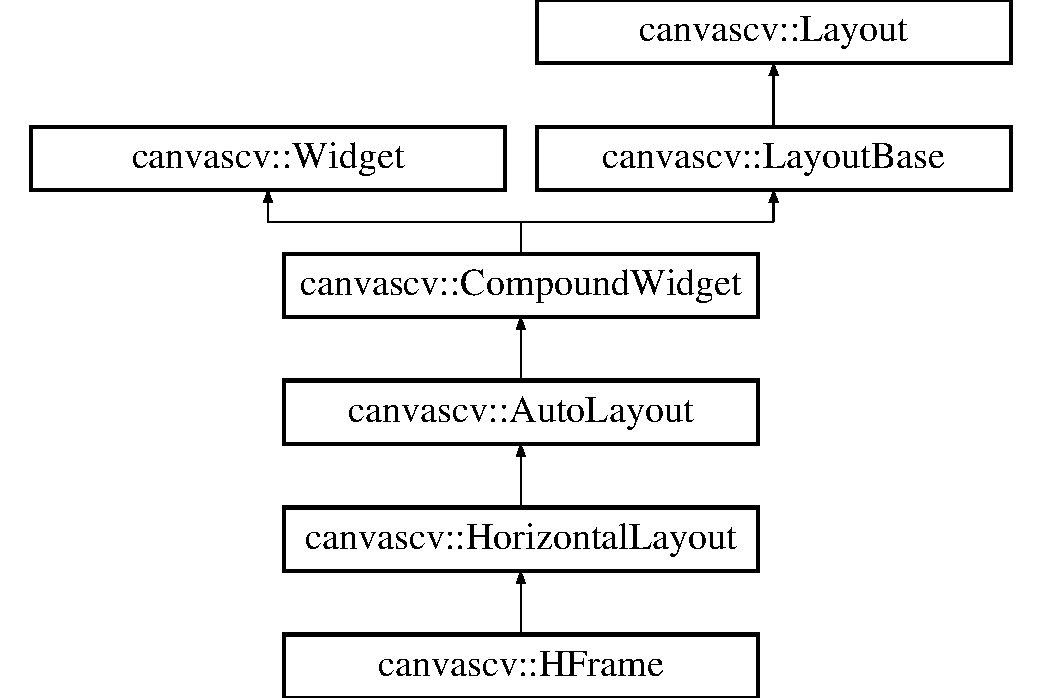
\includegraphics[height=6.000000cm]{classcanvascv_1_1HFrame}
\end{center}
\end{figure}
\subsection*{Public Member Functions}
\begin{DoxyCompactItemize}
\item 
void \hyperlink{classcanvascv_1_1HFrame_a7daeeda5533657170a35bdf78baf511c}{set\+Frame\+Relief} (\hyperlink{classcanvascv_1_1Widget_a8253daa509c55c24c92ce0d3dd93e4cd}{Relief} value)
\begin{DoxyCompactList}\small\item\em set\+Frame\+Relief \end{DoxyCompactList}\item 
virtual const char $\ast$ \hyperlink{classcanvascv_1_1HFrame_a32535b523b26b4db03f46a59fda8237a}{get\+Type} () const 
\begin{DoxyCompactList}\small\item\em get\+Type is always implemented by derived to return the same static pointer per widget. \end{DoxyCompactList}\end{DoxyCompactItemize}
\subsection*{Static Public Member Functions}
\begin{DoxyCompactItemize}
\item 
static std\+::shared\+\_\+ptr$<$ \hyperlink{classcanvascv_1_1HFrame}{H\+Frame} $>$ \hyperlink{classcanvascv_1_1HFrame_a0bd1d3df07a8c25f48e79048913f85fc}{create} (\hyperlink{classcanvascv_1_1Layout}{Layout} \&layout, const cv\+::\+Point \&pos=cv\+::\+Point(0, 0))
\begin{DoxyCompactList}\small\item\em create a \hyperlink{classcanvascv_1_1HFrame}{H\+Frame} widget \end{DoxyCompactList}\end{DoxyCompactItemize}
\subsection*{Additional Inherited Members}


\subsection{Detailed Description}
A frame with a background of a selected relief type. This is also a \hyperlink{classcanvascv_1_1Layout}{Layout} for other Widgets and it lays them horizontally. \begin{DoxySeeAlso}{See also}
\hyperlink{classcanvascv_1_1HorizontalLayout}{Horizontal\+Layout} 
\end{DoxySeeAlso}
\begin{Desc}
\item[Examples\+: ]\par
\hyperlink{example_add_widget_8cpp-example}{example\+\_\+add\+\_\+widget.\+cpp}.\end{Desc}


\subsection{Member Function Documentation}
\index{canvascv\+::\+H\+Frame@{canvascv\+::\+H\+Frame}!create@{create}}
\index{create@{create}!canvascv\+::\+H\+Frame@{canvascv\+::\+H\+Frame}}
\subsubsection[{\texorpdfstring{create(\+Layout \&layout, const cv\+::\+Point \&pos=cv\+::\+Point(0, 0))}{create(Layout &layout, const cv::Point &pos=cv::Point(0, 0))}}]{\setlength{\rightskip}{0pt plus 5cm}static std\+::shared\+\_\+ptr$<${\bf H\+Frame}$>$ canvascv\+::\+H\+Frame\+::create (
\begin{DoxyParamCaption}
\item[{{\bf Layout} \&}]{layout, }
\item[{const cv\+::\+Point \&}]{pos = {\ttfamily cv\+:\+:Point(0,~0)}}
\end{DoxyParamCaption}
)\hspace{0.3cm}{\ttfamily [static]}}\hypertarget{classcanvascv_1_1HFrame_a0bd1d3df07a8c25f48e79048913f85fc}{}\label{classcanvascv_1_1HFrame_a0bd1d3df07a8c25f48e79048913f85fc}

\begin{DoxyParams}{Parameters}
{\em layout} & widgets are placed in layouts Canvas/\+V\+Frame/\+H\+Frame/... \\
\hline
{\em pos} & location in the \hyperlink{classcanvascv_1_1Layout}{Layout} (Layouts can ignore that) \\
\hline
\end{DoxyParams}
\begin{DoxyReturn}{Returns}
a smart pointer copy of the object kept in the \hyperlink{classcanvascv_1_1Layout}{Layout} 
\end{DoxyReturn}
\begin{Desc}
\item[Examples\+: ]\par
\hyperlink{example_add_widget_8cpp-example}{example\+\_\+add\+\_\+widget.\+cpp}, and \hyperlink{example_shapes_widgets_8cpp-example}{example\+\_\+shapes\+\_\+widgets.\+cpp}.\end{Desc}
\index{canvascv\+::\+H\+Frame@{canvascv\+::\+H\+Frame}!get\+Type@{get\+Type}}
\index{get\+Type@{get\+Type}!canvascv\+::\+H\+Frame@{canvascv\+::\+H\+Frame}}
\subsubsection[{\texorpdfstring{get\+Type() const }{getType() const }}]{\setlength{\rightskip}{0pt plus 5cm}virtual const char$\ast$ canvascv\+::\+H\+Frame\+::get\+Type (
\begin{DoxyParamCaption}
{}
\end{DoxyParamCaption}
) const\hspace{0.3cm}{\ttfamily [virtual]}}\hypertarget{classcanvascv_1_1HFrame_a32535b523b26b4db03f46a59fda8237a}{}\label{classcanvascv_1_1HFrame_a32535b523b26b4db03f46a59fda8237a}
\begin{DoxyReturn}{Returns}
const char $\ast$ pointer to string with widget type name 
\end{DoxyReturn}


Reimplemented from \hyperlink{classcanvascv_1_1HorizontalLayout_a7ccafb8692a2a63eb645e9a9c6b2b9b8}{canvascv\+::\+Horizontal\+Layout}.

\index{canvascv\+::\+H\+Frame@{canvascv\+::\+H\+Frame}!set\+Frame\+Relief@{set\+Frame\+Relief}}
\index{set\+Frame\+Relief@{set\+Frame\+Relief}!canvascv\+::\+H\+Frame@{canvascv\+::\+H\+Frame}}
\subsubsection[{\texorpdfstring{set\+Frame\+Relief(\+Relief value)}{setFrameRelief(Relief value)}}]{\setlength{\rightskip}{0pt plus 5cm}void canvascv\+::\+H\+Frame\+::set\+Frame\+Relief (
\begin{DoxyParamCaption}
\item[{{\bf Relief}}]{value}
\end{DoxyParamCaption}
)}\hypertarget{classcanvascv_1_1HFrame_a7daeeda5533657170a35bdf78baf511c}{}\label{classcanvascv_1_1HFrame_a7daeeda5533657170a35bdf78baf511c}

\begin{DoxyParams}{Parameters}
{\em value} & is one of the supported relief types \\
\hline
\end{DoxyParams}
\begin{DoxySeeAlso}{See also}
\hyperlink{classcanvascv_1_1Widget_a8253daa509c55c24c92ce0d3dd93e4cd}{Widget\+::\+Relief} 
\end{DoxySeeAlso}


The documentation for this class was generated from the following file\+:\begin{DoxyCompactItemize}
\item 
Canvas\+C\+V-\/doxygen/src/canvascv/widgets/hframe.\+h\end{DoxyCompactItemize}

\hypertarget{classcanvascv_1_1HorizontalLayout}{}\section{canvascv\+:\+:Horizontal\+Layout Class Reference}
\label{classcanvascv_1_1HorizontalLayout}\index{canvascv\+::\+Horizontal\+Layout@{canvascv\+::\+Horizontal\+Layout}}


The \hyperlink{classcanvascv_1_1HorizontalLayout}{Horizontal\+Layout} class.  




{\ttfamily \#include $<$horizontallayout.\+h$>$}

Inheritance diagram for canvascv\+:\+:Horizontal\+Layout\+:\begin{figure}[H]
\begin{center}
\leavevmode
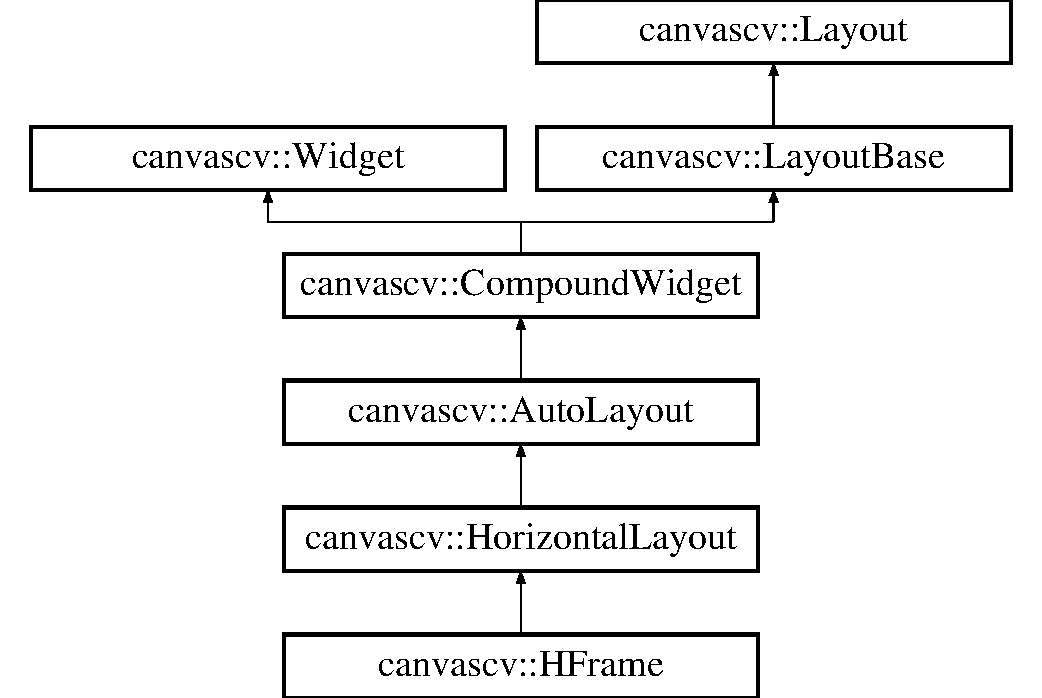
\includegraphics[height=6.000000cm]{classcanvascv_1_1HorizontalLayout}
\end{center}
\end{figure}
\subsection*{Public Member Functions}
\begin{DoxyCompactItemize}
\item 
virtual const char $\ast$ \hyperlink{classcanvascv_1_1HorizontalLayout_a7ccafb8692a2a63eb645e9a9c6b2b9b8}{get\+Type} () const 
\begin{DoxyCompactList}\small\item\em get\+Type is always implemented by derived to return the same static pointer per widget. \end{DoxyCompactList}\item 
int \hyperlink{classcanvascv_1_1HorizontalLayout_aefc6e2cc382de2755233f599bacbed16}{get\+Spacing} () const \hypertarget{classcanvascv_1_1HorizontalLayout_aefc6e2cc382de2755233f599bacbed16}{}\label{classcanvascv_1_1HorizontalLayout_aefc6e2cc382de2755233f599bacbed16}

\begin{DoxyCompactList}\small\item\em returns pixel spacing between items \end{DoxyCompactList}\item 
void \hyperlink{classcanvascv_1_1HorizontalLayout_ad00d6013c170b992322d8d7bfb9e50db}{set\+Spacing} (int value)\hypertarget{classcanvascv_1_1HorizontalLayout_ad00d6013c170b992322d8d7bfb9e50db}{}\label{classcanvascv_1_1HorizontalLayout_ad00d6013c170b992322d8d7bfb9e50db}

\begin{DoxyCompactList}\small\item\em sets pixel spacing between items \end{DoxyCompactList}\end{DoxyCompactItemize}
\subsection*{Static Public Member Functions}
\begin{DoxyCompactItemize}
\item 
static std\+::shared\+\_\+ptr$<$ \hyperlink{classcanvascv_1_1HorizontalLayout}{Horizontal\+Layout} $>$ \hyperlink{classcanvascv_1_1HorizontalLayout_aea31dd787cbf985687ead6a55efa1839}{create} (\hyperlink{classcanvascv_1_1Layout}{Layout} \&layout, const cv\+::\+Point \&pos=cv\+::\+Point(0, 0))
\begin{DoxyCompactList}\small\item\em create a \hyperlink{classcanvascv_1_1HorizontalLayout}{Horizontal\+Layout} widget \end{DoxyCompactList}\end{DoxyCompactItemize}
\subsection*{Protected Member Functions}
\begin{DoxyCompactItemize}
\item 
virtual void \hyperlink{classcanvascv_1_1HorizontalLayout_ab6e59f3499bde32be889d3898cdf6888}{recalc\+Compound} ()
\begin{DoxyCompactList}\small\item\em recalc\+Compound \end{DoxyCompactList}\end{DoxyCompactItemize}
\subsection*{Additional Inherited Members}


\subsection{Detailed Description}
A \hyperlink{classcanvascv_1_1Layout}{Layout} implementation which lays it\textquotesingle{}s internal widgets horizontally with a predefined spacing between widgets.
\begin{DoxyItemize}
\item Horizontal layout is automatic according to widget size and spacing.
\begin{DoxyEnumerate}
\item This layout can expand left (it\textquotesingle{}s \textquotesingle{}flow\+Anchor\textquotesingle{} is R\+I\+G\+HT), or left (it\textquotesingle{}s \textquotesingle{}flow\+Anchor\textquotesingle{} is R\+I\+G\+HT)
\end{DoxyEnumerate}
\item Vertical layout per laid widget is determined according to the laid widget \textquotesingle{}layout\+Anchor\textquotesingle{}\+:
\begin{DoxyEnumerate}
\item T\+OP will align the widget to the top (unless \hyperlink{classcanvascv_1_1Widget_a3ef50b76d33c332cea4e632346b6df33}{set\+Stretch\+Y()} is true in the laid widget)
\item C\+E\+N\+T\+ER will align the widget to the center (unless \hyperlink{classcanvascv_1_1Widget_a3ef50b76d33c332cea4e632346b6df33}{set\+Stretch\+Y()} is true in the laid widget)
\item B\+O\+T\+T\+OM will align the widget to the bottom (unless \hyperlink{classcanvascv_1_1Widget_a3ef50b76d33c332cea4e632346b6df33}{set\+Stretch\+Y()} is true in the laid widget) \begin{DoxyVerb}       layoutAnchor=whatever...(highest sets the standard for other)
           ^
           |
   +-------------------------------------------------------------------------------+
   |       PADDING            PADDING            PADDING            PADDING        |
   | P +--------------+ S +--------------+ S                  S                  P |
   | A |              | P |    Widget    | P +--------------+ P                  A |
   | D |    Widget    | A +--------------+ A |    Widget    | A                  D |
   | D |              | C                  C |              | C +--------------+ D |
   | I |              | I                  I +--------------+ I |    Widget    | I |
   | N +--------------+ N                  N                  N +--------------+ N |
   | G     PADDING      G     PADDING      G     PADDING      G     PADDING      G |
   +-------------------------------------------------------------------------------+
                         layoutAnchor=TOP   layoutAnchor=CENTER layoutAnchor=BOTTOM
\end{DoxyVerb}
 
\end{DoxyEnumerate}
\end{DoxyItemize}

\subsection{Member Function Documentation}
\index{canvascv\+::\+Horizontal\+Layout@{canvascv\+::\+Horizontal\+Layout}!create@{create}}
\index{create@{create}!canvascv\+::\+Horizontal\+Layout@{canvascv\+::\+Horizontal\+Layout}}
\subsubsection[{\texorpdfstring{create(\+Layout \&layout, const cv\+::\+Point \&pos=cv\+::\+Point(0, 0))}{create(Layout &layout, const cv::Point &pos=cv::Point(0, 0))}}]{\setlength{\rightskip}{0pt plus 5cm}static std\+::shared\+\_\+ptr$<${\bf Horizontal\+Layout}$>$ canvascv\+::\+Horizontal\+Layout\+::create (
\begin{DoxyParamCaption}
\item[{{\bf Layout} \&}]{layout, }
\item[{const cv\+::\+Point \&}]{pos = {\ttfamily cv\+:\+:Point(0,~0)}}
\end{DoxyParamCaption}
)\hspace{0.3cm}{\ttfamily [static]}}\hypertarget{classcanvascv_1_1HorizontalLayout_aea31dd787cbf985687ead6a55efa1839}{}\label{classcanvascv_1_1HorizontalLayout_aea31dd787cbf985687ead6a55efa1839}

\begin{DoxyParams}{Parameters}
{\em layout} & widgets are placed in layouts Canvas/\+V\+Frame/\+H\+Frame/... \\
\hline
{\em pos} & location in the \hyperlink{classcanvascv_1_1Layout}{Layout} (Layouts can ignore that) \\
\hline
\end{DoxyParams}
\begin{DoxyReturn}{Returns}
a smart pointer copy of the object kept in the \hyperlink{classcanvascv_1_1Layout}{Layout} 
\end{DoxyReturn}
\begin{Desc}
\item[Examples\+: ]\par
\hyperlink{example_add_widget_8cpp-example}{example\+\_\+add\+\_\+widget.\+cpp}.\end{Desc}
\index{canvascv\+::\+Horizontal\+Layout@{canvascv\+::\+Horizontal\+Layout}!get\+Type@{get\+Type}}
\index{get\+Type@{get\+Type}!canvascv\+::\+Horizontal\+Layout@{canvascv\+::\+Horizontal\+Layout}}
\subsubsection[{\texorpdfstring{get\+Type() const }{getType() const }}]{\setlength{\rightskip}{0pt plus 5cm}virtual const char$\ast$ canvascv\+::\+Horizontal\+Layout\+::get\+Type (
\begin{DoxyParamCaption}
{}
\end{DoxyParamCaption}
) const\hspace{0.3cm}{\ttfamily [virtual]}}\hypertarget{classcanvascv_1_1HorizontalLayout_a7ccafb8692a2a63eb645e9a9c6b2b9b8}{}\label{classcanvascv_1_1HorizontalLayout_a7ccafb8692a2a63eb645e9a9c6b2b9b8}
\begin{DoxyReturn}{Returns}
const char $\ast$ pointer to string with widget type name 
\end{DoxyReturn}


Implements \hyperlink{classcanvascv_1_1Widget_a85884269bd53ab91203f099a586efa43}{canvascv\+::\+Widget}.



Reimplemented in \hyperlink{classcanvascv_1_1HFrame_a32535b523b26b4db03f46a59fda8237a}{canvascv\+::\+H\+Frame}.

\index{canvascv\+::\+Horizontal\+Layout@{canvascv\+::\+Horizontal\+Layout}!recalc\+Compound@{recalc\+Compound}}
\index{recalc\+Compound@{recalc\+Compound}!canvascv\+::\+Horizontal\+Layout@{canvascv\+::\+Horizontal\+Layout}}
\subsubsection[{\texorpdfstring{recalc\+Compound()}{recalcCompound()}}]{\setlength{\rightskip}{0pt plus 5cm}virtual void canvascv\+::\+Horizontal\+Layout\+::recalc\+Compound (
\begin{DoxyParamCaption}
{}
\end{DoxyParamCaption}
)\hspace{0.3cm}{\ttfamily [protected]}, {\ttfamily [virtual]}}\hypertarget{classcanvascv_1_1HorizontalLayout_ab6e59f3499bde32be889d3898cdf6888}{}\label{classcanvascv_1_1HorizontalLayout_ab6e59f3499bde32be889d3898cdf6888}
Your BG size recalculation/allocation and FG drawing is done here. It is done semi automatically. Is you invoke setters in this method on your internal widgets, then make sure to update them and/or their layout 

Implements \hyperlink{classcanvascv_1_1CompoundWidget_a4a4f8241d6fd187ffcae2c7968f13864}{canvascv\+::\+Compound\+Widget}.



The documentation for this class was generated from the following file\+:\begin{DoxyCompactItemize}
\item 
Canvas\+C\+V-\/doxygen/src/canvascv/widgets/horizontallayout.\+h\end{DoxyCompactItemize}

\hypertarget{classcanvascv_1_1LabeledShapesConnector}{}\section{canvascv\+:\+:Labeled\+Shapes\+Connector Class Reference}
\label{classcanvascv_1_1LabeledShapesConnector}\index{canvascv\+::\+Labeled\+Shapes\+Connector@{canvascv\+::\+Labeled\+Shapes\+Connector}}


The \hyperlink{classcanvascv_1_1LabeledShapesConnector}{Labeled\+Shapes\+Connector} class.  




{\ttfamily \#include $<$labeledshapesconnector.\+h$>$}

Inheritance diagram for canvascv\+:\+:Labeled\+Shapes\+Connector\+:\begin{figure}[H]
\begin{center}
\leavevmode
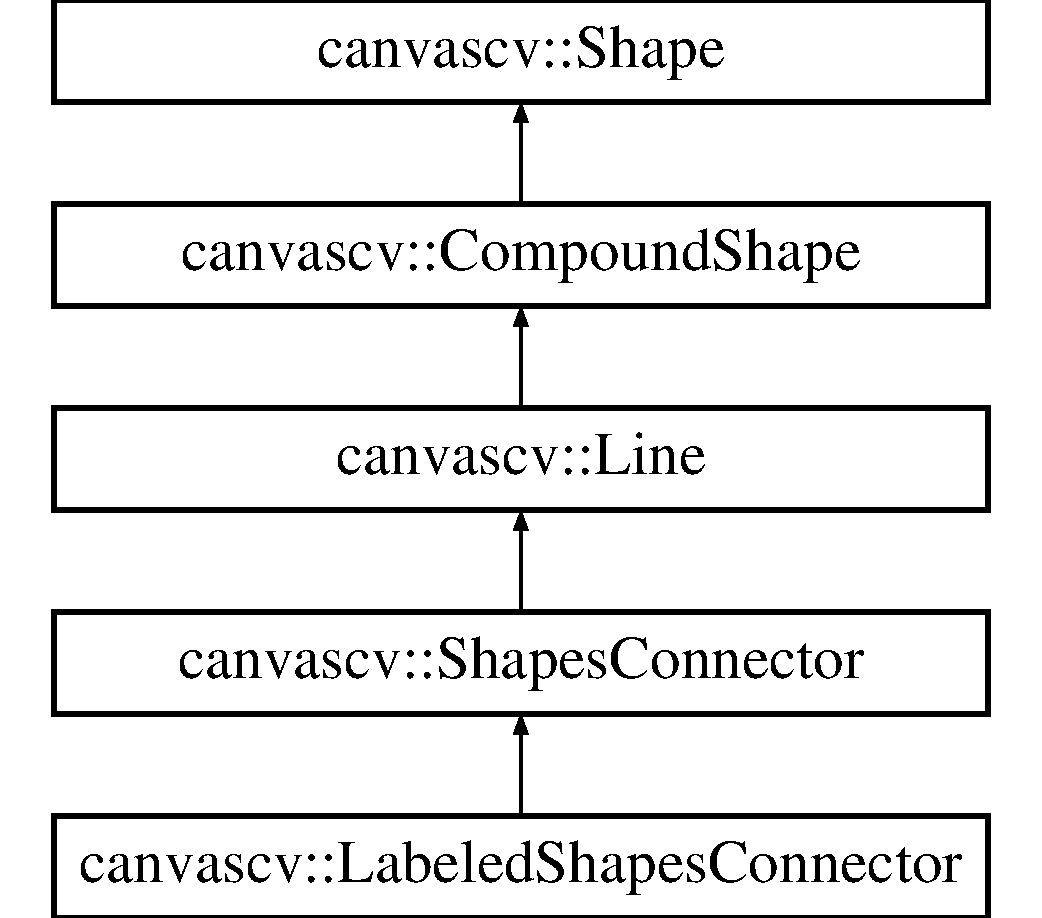
\includegraphics[height=5.000000cm]{classcanvascv_1_1LabeledShapesConnector}
\end{center}
\end{figure}
\subsection*{Public Member Functions}
\begin{DoxyCompactItemize}
\item 
virtual const char $\ast$ \hyperlink{classcanvascv_1_1LabeledShapesConnector_aebeccdf1e7c4efb0bde504b361eac801}{get\+Type} () const 
\begin{DoxyCompactList}\small\item\em get\+Type is always implemented by derived to return the same static pointer per shape. \end{DoxyCompactList}\end{DoxyCompactItemize}
\subsection*{Additional Inherited Members}


\subsection{Detailed Description}
Allows visually connecting 2 shapes from the code or by mouse. There is an additional label (aka \hyperlink{classcanvascv_1_1TextBox}{Text\+Box}) for this type. 

\subsection{Member Function Documentation}
\index{canvascv\+::\+Labeled\+Shapes\+Connector@{canvascv\+::\+Labeled\+Shapes\+Connector}!get\+Type@{get\+Type}}
\index{get\+Type@{get\+Type}!canvascv\+::\+Labeled\+Shapes\+Connector@{canvascv\+::\+Labeled\+Shapes\+Connector}}
\subsubsection[{\texorpdfstring{get\+Type() const }{getType() const }}]{\setlength{\rightskip}{0pt plus 5cm}virtual const char$\ast$ canvascv\+::\+Labeled\+Shapes\+Connector\+::get\+Type (
\begin{DoxyParamCaption}
{}
\end{DoxyParamCaption}
) const\hspace{0.3cm}{\ttfamily [virtual]}}\hypertarget{classcanvascv_1_1LabeledShapesConnector_aebeccdf1e7c4efb0bde504b361eac801}{}\label{classcanvascv_1_1LabeledShapesConnector_aebeccdf1e7c4efb0bde504b361eac801}
\begin{DoxyReturn}{Returns}
const char $\ast$ pointer to string with shape type name 
\end{DoxyReturn}


Reimplemented from \hyperlink{classcanvascv_1_1ShapesConnector_aedda9e8fd9c1be85704f289df94905a2}{canvascv\+::\+Shapes\+Connector}.



The documentation for this class was generated from the following file\+:\begin{DoxyCompactItemize}
\item 
Canvas\+C\+V-\/doxygen/src/canvascv/shapes/labeledshapesconnector.\+h\end{DoxyCompactItemize}

\hypertarget{classcanvascv_1_1Layout}{}\section{canvascv\+:\+:Layout Class Reference}
\label{classcanvascv_1_1Layout}\index{canvascv\+::\+Layout@{canvascv\+::\+Layout}}


The \hyperlink{classcanvascv_1_1Layout}{Layout} class.  




{\ttfamily \#include $<$layout.\+h$>$}

Inheritance diagram for canvascv\+:\+:Layout\+:\begin{figure}[H]
\begin{center}
\leavevmode
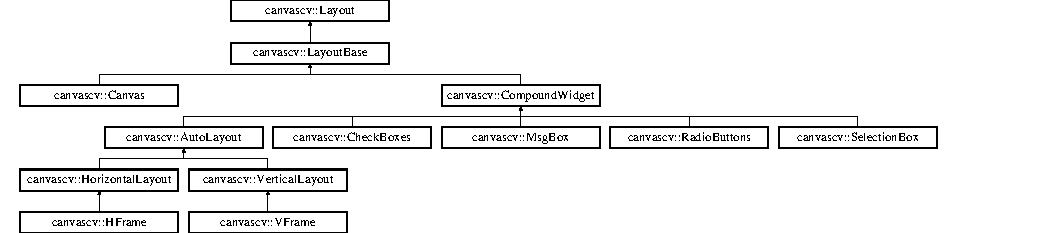
\includegraphics[height=3.128491cm]{classcanvascv_1_1Layout}
\end{center}
\end{figure}
\subsection*{Protected Member Functions}
\begin{DoxyCompactItemize}
\item 
virtual void \hyperlink{classcanvascv_1_1Layout_a90b4264dce5634f09d555c22358e35f0}{add\+Widget} (const std\+::shared\+\_\+ptr$<$ \hyperlink{classcanvascv_1_1Widget}{Widget} $>$ \&widget)=0\hypertarget{classcanvascv_1_1Layout_a90b4264dce5634f09d555c22358e35f0}{}\label{classcanvascv_1_1Layout_a90b4264dce5634f09d555c22358e35f0}

\begin{DoxyCompactList}\small\item\em adds the widget to this \hyperlink{classcanvascv_1_1Layout}{Layout} after removing it from it\textquotesingle{}s previous layout \end{DoxyCompactList}\item 
virtual std\+::shared\+\_\+ptr$<$ \hyperlink{classcanvascv_1_1Widget}{Widget} $>$ \hyperlink{classcanvascv_1_1Layout_a7b532816232c436ea5b6e7c4c3254779}{rmv\+Widget} (const std\+::shared\+\_\+ptr$<$ \hyperlink{classcanvascv_1_1Widget}{Widget} $>$ \&widget)=0
\begin{DoxyCompactList}\small\item\em rmv\+Widget \end{DoxyCompactList}\end{DoxyCompactItemize}


\subsection{Detailed Description}
This is the layout interface class. All widgets must go into a \hyperlink{classcanvascv_1_1Layout}{Layout}. All Layouts are also widgets except for the \hyperlink{classcanvascv_1_1Canvas}{Canvas} class. \begin{Desc}
\item[Examples\+: ]\par
\hyperlink{example_add_widget_8cpp-example}{example\+\_\+add\+\_\+widget.\+cpp}.\end{Desc}


\subsection{Member Function Documentation}
\index{canvascv\+::\+Layout@{canvascv\+::\+Layout}!rmv\+Widget@{rmv\+Widget}}
\index{rmv\+Widget@{rmv\+Widget}!canvascv\+::\+Layout@{canvascv\+::\+Layout}}
\subsubsection[{\texorpdfstring{rmv\+Widget(const std\+::shared\+\_\+ptr$<$ Widget $>$ \&widget)=0}{rmvWidget(const std::shared_ptr< Widget > &widget)=0}}]{\setlength{\rightskip}{0pt plus 5cm}virtual std\+::shared\+\_\+ptr$<${\bf Widget}$>$ canvascv\+::\+Layout\+::rmv\+Widget (
\begin{DoxyParamCaption}
\item[{const std\+::shared\+\_\+ptr$<$ {\bf Widget} $>$ \&}]{widget}
\end{DoxyParamCaption}
)\hspace{0.3cm}{\ttfamily [protected]}, {\ttfamily [pure virtual]}}\hypertarget{classcanvascv_1_1Layout_a7b532816232c436ea5b6e7c4c3254779}{}\label{classcanvascv_1_1Layout_a7b532816232c436ea5b6e7c4c3254779}

\begin{DoxyParams}{Parameters}
{\em widget} & will be removed from this \hyperlink{classcanvascv_1_1Layout}{Layout} \\
\hline
\end{DoxyParams}
\begin{DoxyReturn}{Returns}
filled shared\+\_\+ptr to removed widget or empty if not found 
\end{DoxyReturn}
\begin{DoxyNote}{Note}
Widgets must be in layouts to be displayed correctly. 
\end{DoxyNote}


Implemented in \hyperlink{classcanvascv_1_1Canvas_a70248a9be2eedcacad74c9be5fd615eb}{canvascv\+::\+Canvas}, \hyperlink{classcanvascv_1_1CompoundWidget_ad4a37bf31f9cf6410b41526a5b83c75a}{canvascv\+::\+Compound\+Widget}, and \hyperlink{classcanvascv_1_1AutoLayout_abc436c90f50a5331c391e351bef9e659}{canvascv\+::\+Auto\+Layout}.



The documentation for this class was generated from the following file\+:\begin{DoxyCompactItemize}
\item 
Canvas\+C\+V-\/doxygen/src/canvascv/widgets/layout.\+h\end{DoxyCompactItemize}

\hypertarget{classcanvascv_1_1LayoutBase}{}\section{canvascv\+:\+:Layout\+Base Class Reference}
\label{classcanvascv_1_1LayoutBase}\index{canvascv\+::\+Layout\+Base@{canvascv\+::\+Layout\+Base}}


The \hyperlink{classcanvascv_1_1LayoutBase}{Layout\+Base} class.  




{\ttfamily \#include $<$layoutbase.\+h$>$}

Inheritance diagram for canvascv\+:\+:Layout\+Base\+:\begin{figure}[H]
\begin{center}
\leavevmode
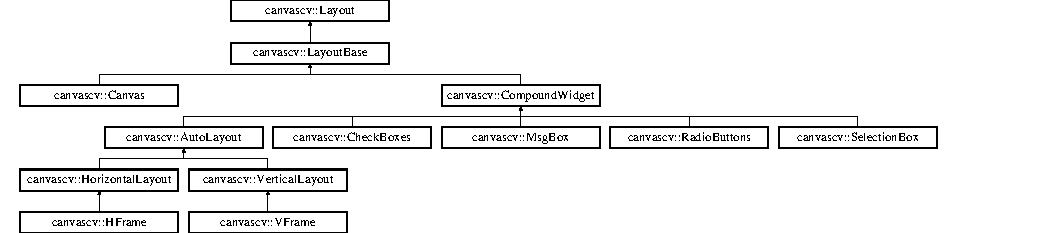
\includegraphics[height=3.128491cm]{classcanvascv_1_1LayoutBase}
\end{center}
\end{figure}
\subsection*{Additional Inherited Members}


\subsection{Detailed Description}
Common base class for all \hyperlink{classcanvascv_1_1Layout}{Layout} classes 

The documentation for this class was generated from the following file\+:\begin{DoxyCompactItemize}
\item 
Canvas\+C\+V-\/doxygen/src/canvascv/widgets/layoutbase.\+h\end{DoxyCompactItemize}

\hypertarget{classcanvascv_1_1Line}{}\section{canvascv\+:\+:Line Class Reference}
\label{classcanvascv_1_1Line}\index{canvascv\+::\+Line@{canvascv\+::\+Line}}


The \hyperlink{classcanvascv_1_1Line}{Line} class.  




{\ttfamily \#include $<$line.\+h$>$}

Inheritance diagram for canvascv\+:\+:Line\+:\begin{figure}[H]
\begin{center}
\leavevmode
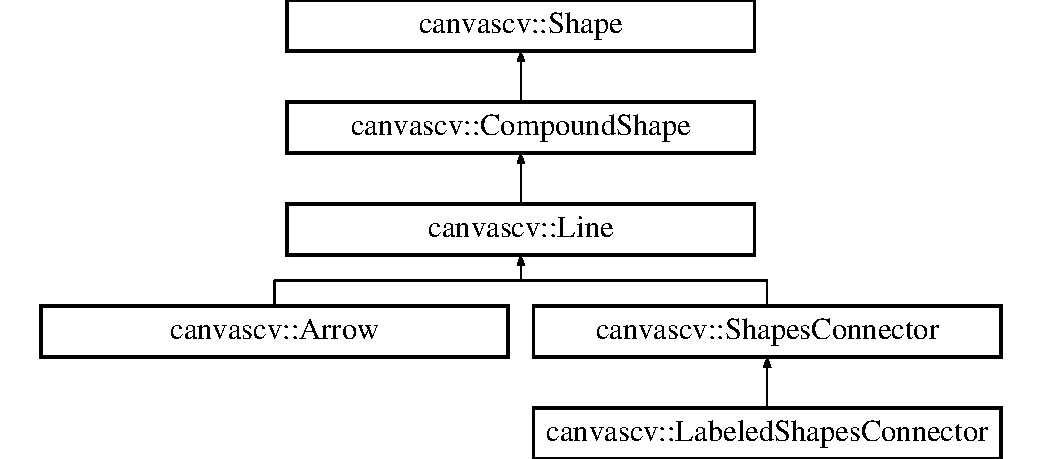
\includegraphics[height=5.000000cm]{classcanvascv_1_1Line}
\end{center}
\end{figure}
\subsection*{Public Member Functions}
\begin{DoxyCompactItemize}
\item 
void \hyperlink{classcanvascv_1_1Line_ad58eb26a9f759fcef069ef088eda016a}{lock\+Tail} (bool is\+Locked)\hypertarget{classcanvascv_1_1Line_ad58eb26a9f759fcef069ef088eda016a}{}\label{classcanvascv_1_1Line_ad58eb26a9f759fcef069ef088eda016a}

\begin{DoxyCompactList}\small\item\em set if to lock the tail (\hyperlink{classcanvascv_1_1Handle}{Handle}) of the line \end{DoxyCompactList}\item 
void \hyperlink{classcanvascv_1_1Line_a7ed04307f5469a0f3dbb56843e4def30}{lock\+Head} (bool is\+Locked)\hypertarget{classcanvascv_1_1Line_a7ed04307f5469a0f3dbb56843e4def30}{}\label{classcanvascv_1_1Line_a7ed04307f5469a0f3dbb56843e4def30}

\begin{DoxyCompactList}\small\item\em set if to lock the head (\hyperlink{classcanvascv_1_1Handle}{Handle}) of the line \end{DoxyCompactList}\item 
void \hyperlink{classcanvascv_1_1Line_ad8792291c57126a5ce100cc53c58ad59}{show\+Tail} (bool is\+Visible)\hypertarget{classcanvascv_1_1Line_ad8792291c57126a5ce100cc53c58ad59}{}\label{classcanvascv_1_1Line_ad8792291c57126a5ce100cc53c58ad59}

\begin{DoxyCompactList}\small\item\em set if to show the tail (\hyperlink{classcanvascv_1_1Handle}{Handle}) of the line \end{DoxyCompactList}\item 
void \hyperlink{classcanvascv_1_1Line_a606cc47470a49cb689f9a536d019552e}{show\+Head} (bool is\+Visible)\hypertarget{classcanvascv_1_1Line_a606cc47470a49cb689f9a536d019552e}{}\label{classcanvascv_1_1Line_a606cc47470a49cb689f9a536d019552e}

\begin{DoxyCompactList}\small\item\em set if to show the head (\hyperlink{classcanvascv_1_1Handle}{Handle}) of the line \end{DoxyCompactList}\item 
void \hyperlink{classcanvascv_1_1Line_a51eccef05df0ea69f99ee9eca3f3b12c}{set\+Tail\+Pos} (const cv\+::\+Point \&pos)\hypertarget{classcanvascv_1_1Line_a51eccef05df0ea69f99ee9eca3f3b12c}{}\label{classcanvascv_1_1Line_a51eccef05df0ea69f99ee9eca3f3b12c}

\begin{DoxyCompactList}\small\item\em will move the tail (\hyperlink{classcanvascv_1_1Handle}{Handle}) of the line to pos \end{DoxyCompactList}\item 
void \hyperlink{classcanvascv_1_1Line_a0aa66e5c23a5c1173786f6c7c9519bfa}{set\+Head\+Pos} (const cv\+::\+Point \&pos)\hypertarget{classcanvascv_1_1Line_a0aa66e5c23a5c1173786f6c7c9519bfa}{}\label{classcanvascv_1_1Line_a0aa66e5c23a5c1173786f6c7c9519bfa}

\begin{DoxyCompactList}\small\item\em will move the head (\hyperlink{classcanvascv_1_1Handle}{Handle}) of the line to pos \end{DoxyCompactList}\item 
double \hyperlink{classcanvascv_1_1Line_a7a076a5ac4f7f4aa99e0323daa04677c}{length} () const \hypertarget{classcanvascv_1_1Line_a7a076a5ac4f7f4aa99e0323daa04677c}{}\label{classcanvascv_1_1Line_a7a076a5ac4f7f4aa99e0323daa04677c}

\begin{DoxyCompactList}\small\item\em returns the length of the line in pixels \end{DoxyCompactList}\item 
bool \hyperlink{classcanvascv_1_1Line_a4b7e7bc0c752743768e9d0e850c27288}{is\+Point\+On\+Line} (const cv\+::\+Point \&p3, int threshold=3) const \hypertarget{classcanvascv_1_1Line_a4b7e7bc0c752743768e9d0e850c27288}{}\label{classcanvascv_1_1Line_a4b7e7bc0c752743768e9d0e850c27288}

\begin{DoxyCompactList}\small\item\em returns true if the point \textquotesingle{}p3\textquotesingle{} is on the line, give or take \textquotesingle{}threshold\textquotesingle{} pixels \end{DoxyCompactList}\item 
\hyperlink{classcanvascv_1_1Handle}{Handle} \& \hyperlink{classcanvascv_1_1Line_a685abcca89d05c63186ef71c0ef8b0a2}{get\+P\+T1} ()\hypertarget{classcanvascv_1_1Line_a685abcca89d05c63186ef71c0ef8b0a2}{}\label{classcanvascv_1_1Line_a685abcca89d05c63186ef71c0ef8b0a2}

\begin{DoxyCompactList}\small\item\em get the \hyperlink{classcanvascv_1_1Handle}{Handle} to the tail of the \end{DoxyCompactList}\item 
\hyperlink{classcanvascv_1_1Handle}{Handle} \& \hyperlink{classcanvascv_1_1Line_a7a0fc9d06ab0fc575b1596068dff0484}{get\+P\+T2} ()\hypertarget{classcanvascv_1_1Line_a7a0fc9d06ab0fc575b1596068dff0484}{}\label{classcanvascv_1_1Line_a7a0fc9d06ab0fc575b1596068dff0484}

\begin{DoxyCompactList}\small\item\em get the \hyperlink{classcanvascv_1_1Handle}{Handle} to the head of the \end{DoxyCompactList}\item 
const cv\+::\+Point \& \hyperlink{classcanvascv_1_1Line_a0f3a3d49c01ac13e45496f197a0b0ab8}{get\+Tail} () const \hypertarget{classcanvascv_1_1Line_a0f3a3d49c01ac13e45496f197a0b0ab8}{}\label{classcanvascv_1_1Line_a0f3a3d49c01ac13e45496f197a0b0ab8}

\begin{DoxyCompactList}\small\item\em get the Point position og the tail \hyperlink{classcanvascv_1_1Handle}{Handle} \end{DoxyCompactList}\item 
const cv\+::\+Point \& \hyperlink{classcanvascv_1_1Line_aa0dfcc4fcfbc07eefac5b962f12c7fb0}{get\+Head} () const \hypertarget{classcanvascv_1_1Line_aa0dfcc4fcfbc07eefac5b962f12c7fb0}{}\label{classcanvascv_1_1Line_aa0dfcc4fcfbc07eefac5b962f12c7fb0}

\begin{DoxyCompactList}\small\item\em get the Point position og the head \hyperlink{classcanvascv_1_1Handle}{Handle} \end{DoxyCompactList}\item 
virtual bool \hyperlink{classcanvascv_1_1Line_aa7bd63d71cc0f63cef68b397c0c24168}{is\+At\+Pos} (const cv\+::\+Point \&pos)\hypertarget{classcanvascv_1_1Line_aa7bd63d71cc0f63cef68b397c0c24168}{}\label{classcanvascv_1_1Line_aa7bd63d71cc0f63cef68b397c0c24168}

\begin{DoxyCompactList}\small\item\em returns true if shape is at pos, false otherwise \end{DoxyCompactList}\item 
virtual bool \hyperlink{classcanvascv_1_1Line_a4059736cde05ffc90dda8ed1ff4f9ba2}{key\+Pressed} (int \&key)
\begin{DoxyCompactList}\small\item\em key\+Pressed will be called by \hyperlink{classcanvascv_1_1Canvas}{Canvas} for active shapes \end{DoxyCompactList}\item 
virtual std\+::list$<$ \hyperlink{classcanvascv_1_1Handle}{Handle} $\ast$ $>$ \hyperlink{classcanvascv_1_1Line_a4a4293ae8f9600ee7f9d3a8089e6965a}{get\+Connection\+Targets} ()
\begin{DoxyCompactList}\small\item\em get\+Connection\+Targets \end{DoxyCompactList}\item 
virtual const char $\ast$ \hyperlink{classcanvascv_1_1Line_a863306159fbca892702fd3d0047b63c3}{get\+Type} () const 
\begin{DoxyCompactList}\small\item\em get\+Type is always implemented by derived to return the same static pointer per shape. \end{DoxyCompactList}\end{DoxyCompactItemize}
\subsection*{Protected Member Functions}
\begin{DoxyCompactItemize}
\item 
virtual void \hyperlink{classcanvascv_1_1Line_aad801107019337b6e369fed331539d56}{draw} (cv\+::\+Mat \&canvas)
\begin{DoxyCompactList}\small\item\em draw shape on the canvas \end{DoxyCompactList}\item 
virtual bool \hyperlink{classcanvascv_1_1Line_aab4d23d336fe71c6d7000d8da9a54269}{mouse\+Pressed} (const cv\+::\+Point \&pos, bool on\+Create=false)
\begin{DoxyCompactList}\small\item\em mouse\+Pressed \end{DoxyCompactList}\item 
virtual bool \hyperlink{classcanvascv_1_1Line_ad758464d98d455d2ea3aa591667fb595}{mouse\+Moved} (const cv\+::\+Point \&pos)
\begin{DoxyCompactList}\small\item\em mouse\+Moved \end{DoxyCompactList}\item 
virtual bool \hyperlink{classcanvascv_1_1Line_ace7269cabd2acbb2c9da009740f46fa3}{mouse\+Released} (const cv\+::\+Point \&pos)
\begin{DoxyCompactList}\small\item\em mouse\+Released \end{DoxyCompactList}\end{DoxyCompactItemize}
\subsection*{Additional Inherited Members}


\subsection{Detailed Description}
Allows you to draw a line by mouse or from code 

\subsection{Member Function Documentation}
\index{canvascv\+::\+Line@{canvascv\+::\+Line}!draw@{draw}}
\index{draw@{draw}!canvascv\+::\+Line@{canvascv\+::\+Line}}
\subsubsection[{\texorpdfstring{draw(cv\+::\+Mat \&canvas)}{draw(cv::Mat &canvas)}}]{\setlength{\rightskip}{0pt plus 5cm}virtual void canvascv\+::\+Line\+::draw (
\begin{DoxyParamCaption}
\item[{cv\+::\+Mat \&}]{canvas}
\end{DoxyParamCaption}
)\hspace{0.3cm}{\ttfamily [protected]}, {\ttfamily [virtual]}}\hypertarget{classcanvascv_1_1Line_aad801107019337b6e369fed331539d56}{}\label{classcanvascv_1_1Line_aad801107019337b6e369fed331539d56}

\begin{DoxyParams}{Parameters}
{\em canvas} & \\
\hline
\end{DoxyParams}


Reimplemented from \hyperlink{classcanvascv_1_1CompoundShape_a6ec60ee0340ed25274e3ac1349345953}{canvascv\+::\+Compound\+Shape}.



Reimplemented in \hyperlink{classcanvascv_1_1Arrow_a8ba5b890df49a2d8fc6630df5fe80351}{canvascv\+::\+Arrow}.

\index{canvascv\+::\+Line@{canvascv\+::\+Line}!get\+Connection\+Targets@{get\+Connection\+Targets}}
\index{get\+Connection\+Targets@{get\+Connection\+Targets}!canvascv\+::\+Line@{canvascv\+::\+Line}}
\subsubsection[{\texorpdfstring{get\+Connection\+Targets()}{getConnectionTargets()}}]{\setlength{\rightskip}{0pt plus 5cm}virtual std\+::list$<${\bf Handle} $\ast$$>$ canvascv\+::\+Line\+::get\+Connection\+Targets (
\begin{DoxyParamCaption}
{}
\end{DoxyParamCaption}
)\hspace{0.3cm}{\ttfamily [virtual]}}\hypertarget{classcanvascv_1_1Line_a4a4293ae8f9600ee7f9d3a8089e6965a}{}\label{classcanvascv_1_1Line_a4a4293ae8f9600ee7f9d3a8089e6965a}
Return a list of Handles this shape allows to connect to from other shapes (mainly for \hyperlink{classcanvascv_1_1ShapesConnector}{Shapes\+Connector}) \begin{DoxyReturn}{Returns}
list of \hyperlink{classcanvascv_1_1Handle}{Handle} pointers we \hyperlink{classcanvascv_1_1ShapesConnector}{Shapes\+Connector} can use to connect 
\end{DoxyReturn}


Implements \hyperlink{classcanvascv_1_1Shape_a827822e17e24118e16fa932ac0e71cd2}{canvascv\+::\+Shape}.



Reimplemented in \hyperlink{classcanvascv_1_1ShapesConnector_a90672acd22f69f3d143f08197d4108b8}{canvascv\+::\+Shapes\+Connector}.

\index{canvascv\+::\+Line@{canvascv\+::\+Line}!get\+Type@{get\+Type}}
\index{get\+Type@{get\+Type}!canvascv\+::\+Line@{canvascv\+::\+Line}}
\subsubsection[{\texorpdfstring{get\+Type() const }{getType() const }}]{\setlength{\rightskip}{0pt plus 5cm}virtual const char$\ast$ canvascv\+::\+Line\+::get\+Type (
\begin{DoxyParamCaption}
{}
\end{DoxyParamCaption}
) const\hspace{0.3cm}{\ttfamily [virtual]}}\hypertarget{classcanvascv_1_1Line_a863306159fbca892702fd3d0047b63c3}{}\label{classcanvascv_1_1Line_a863306159fbca892702fd3d0047b63c3}
\begin{DoxyReturn}{Returns}
const char $\ast$ pointer to string with shape type name 
\end{DoxyReturn}


Implements \hyperlink{classcanvascv_1_1Shape_adee3cc696c7e82b0d2946e7e667ddd46}{canvascv\+::\+Shape}.



Reimplemented in \hyperlink{classcanvascv_1_1ShapesConnector_aedda9e8fd9c1be85704f289df94905a2}{canvascv\+::\+Shapes\+Connector}, \hyperlink{classcanvascv_1_1LabeledShapesConnector_aebeccdf1e7c4efb0bde504b361eac801}{canvascv\+::\+Labeled\+Shapes\+Connector}, and \hyperlink{classcanvascv_1_1Arrow_a4d0857dec7276f993bd390e944edef34}{canvascv\+::\+Arrow}.

\index{canvascv\+::\+Line@{canvascv\+::\+Line}!key\+Pressed@{key\+Pressed}}
\index{key\+Pressed@{key\+Pressed}!canvascv\+::\+Line@{canvascv\+::\+Line}}
\subsubsection[{\texorpdfstring{key\+Pressed(int \&key)}{keyPressed(int &key)}}]{\setlength{\rightskip}{0pt plus 5cm}virtual bool canvascv\+::\+Line\+::key\+Pressed (
\begin{DoxyParamCaption}
\item[{int \&}]{key}
\end{DoxyParamCaption}
)\hspace{0.3cm}{\ttfamily [virtual]}}\hypertarget{classcanvascv_1_1Line_a4059736cde05ffc90dda8ed1ff4f9ba2}{}\label{classcanvascv_1_1Line_a4059736cde05ffc90dda8ed1ff4f9ba2}

\begin{DoxyParams}{Parameters}
{\em key} & was pressed. You must set it to -\/1 if you consumed it. \\
\hline
\end{DoxyParams}
\begin{DoxyReturn}{Returns}
true if we want to stay in focus and false otherwise 
\end{DoxyReturn}


Reimplemented from \hyperlink{classcanvascv_1_1CompoundShape_ac739f68737099c6f5c6d2c70196cd07b}{canvascv\+::\+Compound\+Shape}.

\index{canvascv\+::\+Line@{canvascv\+::\+Line}!mouse\+Moved@{mouse\+Moved}}
\index{mouse\+Moved@{mouse\+Moved}!canvascv\+::\+Line@{canvascv\+::\+Line}}
\subsubsection[{\texorpdfstring{mouse\+Moved(const cv\+::\+Point \&pos)}{mouseMoved(const cv::Point &pos)}}]{\setlength{\rightskip}{0pt plus 5cm}virtual bool canvascv\+::\+Line\+::mouse\+Moved (
\begin{DoxyParamCaption}
\item[{const cv\+::\+Point \&}]{pos}
\end{DoxyParamCaption}
)\hspace{0.3cm}{\ttfamily [protected]}, {\ttfamily [virtual]}}\hypertarget{classcanvascv_1_1Line_ad758464d98d455d2ea3aa591667fb595}{}\label{classcanvascv_1_1Line_ad758464d98d455d2ea3aa591667fb595}

\begin{DoxyEnumerate}
\item Was a mouse moved over this shape?
\item If shape is during edit, then these are the mouse position. 
\begin{DoxyParams}{Parameters}
{\em pos} & \\
\hline
\end{DoxyParams}
\begin{DoxyReturn}{Returns}
true if a mouse moved over this shape, or it is during edit. false otherwise. 
\end{DoxyReturn}

\end{DoxyEnumerate}

Reimplemented from \hyperlink{classcanvascv_1_1CompoundShape_a387d1705b99d2053306ffd8d8e67b63b}{canvascv\+::\+Compound\+Shape}.

\index{canvascv\+::\+Line@{canvascv\+::\+Line}!mouse\+Pressed@{mouse\+Pressed}}
\index{mouse\+Pressed@{mouse\+Pressed}!canvascv\+::\+Line@{canvascv\+::\+Line}}
\subsubsection[{\texorpdfstring{mouse\+Pressed(const cv\+::\+Point \&pos, bool on\+Create=false)}{mousePressed(const cv::Point &pos, bool onCreate=false)}}]{\setlength{\rightskip}{0pt plus 5cm}virtual bool canvascv\+::\+Line\+::mouse\+Pressed (
\begin{DoxyParamCaption}
\item[{const cv\+::\+Point \&}]{pos, }
\item[{bool}]{on\+Create = {\ttfamily false}}
\end{DoxyParamCaption}
)\hspace{0.3cm}{\ttfamily [protected]}, {\ttfamily [virtual]}}\hypertarget{classcanvascv_1_1Line_aab4d23d336fe71c6d7000d8da9a54269}{}\label{classcanvascv_1_1Line_aab4d23d336fe71c6d7000d8da9a54269}

\begin{DoxyParams}{Parameters}
{\em pos} & \\
\hline
{\em on\+Create} & is true if this is the mouse press which cerated this shape \\
\hline
\end{DoxyParams}
\begin{DoxyReturn}{Returns}
true for keep in focus, false for leave focus 
\end{DoxyReturn}


Reimplemented from \hyperlink{classcanvascv_1_1CompoundShape_a821d046dceaba47114385d1c87e197ce}{canvascv\+::\+Compound\+Shape}.



Reimplemented in \hyperlink{classcanvascv_1_1ShapesConnector_a6c6400403c6c2809af1e0a64e477f592}{canvascv\+::\+Shapes\+Connector}.

\index{canvascv\+::\+Line@{canvascv\+::\+Line}!mouse\+Released@{mouse\+Released}}
\index{mouse\+Released@{mouse\+Released}!canvascv\+::\+Line@{canvascv\+::\+Line}}
\subsubsection[{\texorpdfstring{mouse\+Released(const cv\+::\+Point \&pos)}{mouseReleased(const cv::Point &pos)}}]{\setlength{\rightskip}{0pt plus 5cm}virtual bool canvascv\+::\+Line\+::mouse\+Released (
\begin{DoxyParamCaption}
\item[{const cv\+::\+Point \&}]{pos}
\end{DoxyParamCaption}
)\hspace{0.3cm}{\ttfamily [protected]}, {\ttfamily [virtual]}}\hypertarget{classcanvascv_1_1Line_ace7269cabd2acbb2c9da009740f46fa3}{}\label{classcanvascv_1_1Line_ace7269cabd2acbb2c9da009740f46fa3}

\begin{DoxyParams}{Parameters}
{\em pos} & \\
\hline
\end{DoxyParams}
\begin{DoxyReturn}{Returns}
true for keep in focus, false for leave focus 
\end{DoxyReturn}


Reimplemented from \hyperlink{classcanvascv_1_1CompoundShape_a01cf027fd5f7ec96525949d0c8ae08a1}{canvascv\+::\+Compound\+Shape}.



Reimplemented in \hyperlink{classcanvascv_1_1ShapesConnector_a56ab827f3d72e495ccfd1101807413f8}{canvascv\+::\+Shapes\+Connector}.



The documentation for this class was generated from the following file\+:\begin{DoxyCompactItemize}
\item 
Canvas\+C\+V-\/doxygen/src/canvascv/shapes/line.\+h\end{DoxyCompactItemize}

\hypertarget{classcanvascv_1_1LineCrossing}{}\section{canvascv\+:\+:Line\+Crossing Class Reference}
\label{classcanvascv_1_1LineCrossing}\index{canvascv\+::\+Line\+Crossing@{canvascv\+::\+Line\+Crossing}}


The \hyperlink{classcanvascv_1_1LineCrossing}{Line\+Crossing} class.  




{\ttfamily \#include $<$linecrossing.\+h$>$}

Inheritance diagram for canvascv\+:\+:Line\+Crossing\+:\begin{figure}[H]
\begin{center}
\leavevmode
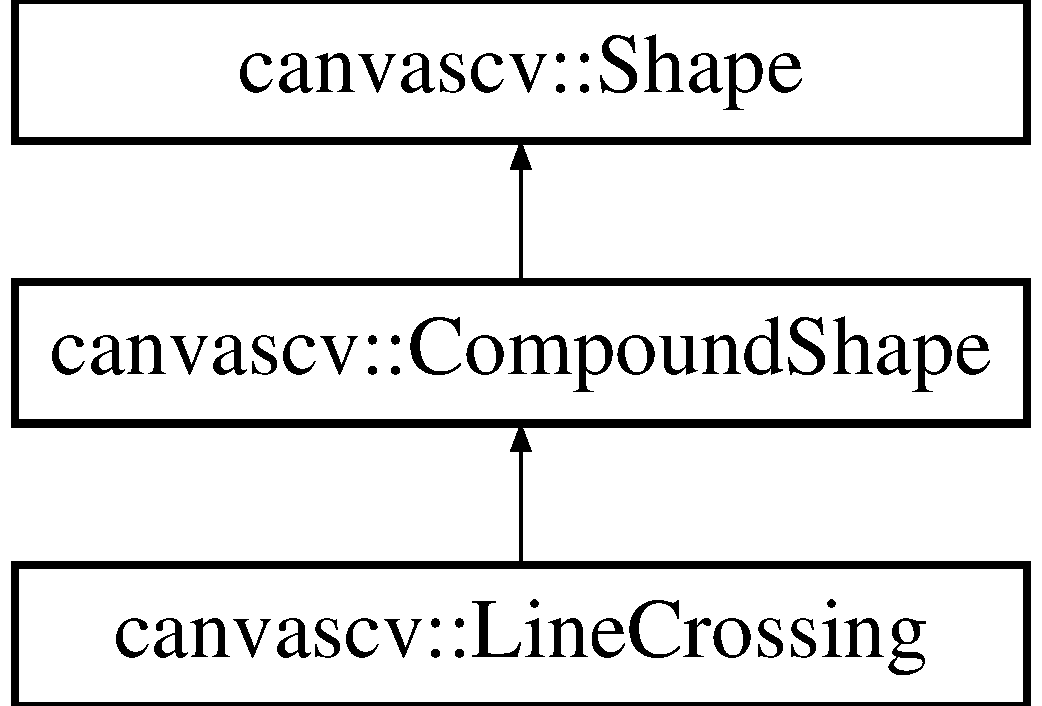
\includegraphics[height=3.000000cm]{classcanvascv_1_1LineCrossing}
\end{center}
\end{figure}
\subsection*{Public Member Functions}
\begin{DoxyCompactItemize}
\item 
int \hyperlink{classcanvascv_1_1LineCrossing_adfd51e0d8d224200b4466627241df4c9}{get\+Direction} () const \hypertarget{classcanvascv_1_1LineCrossing_adfd51e0d8d224200b4466627241df4c9}{}\label{classcanvascv_1_1LineCrossing_adfd51e0d8d224200b4466627241df4c9}

\begin{DoxyCompactList}\small\item\em -\/1 or 1 \end{DoxyCompactList}\item 
const std\+::string \& \hyperlink{classcanvascv_1_1LineCrossing_a3a2bdd022bca8469ebdc63572fe86f06}{get\+Name} () const \hypertarget{classcanvascv_1_1LineCrossing_a3a2bdd022bca8469ebdc63572fe86f06}{}\label{classcanvascv_1_1LineCrossing_a3a2bdd022bca8469ebdc63572fe86f06}

\begin{DoxyCompactList}\small\item\em gets the text from the attached \hyperlink{classcanvascv_1_1TextBox}{Text\+Box} \end{DoxyCompactList}\item 
void \hyperlink{classcanvascv_1_1LineCrossing_a577a282941ac95558da70bdcad0623ee}{set\+Name} (const std\+::string \&value) const \hypertarget{classcanvascv_1_1LineCrossing_a577a282941ac95558da70bdcad0623ee}{}\label{classcanvascv_1_1LineCrossing_a577a282941ac95558da70bdcad0623ee}

\begin{DoxyCompactList}\small\item\em sets the text in the attached \hyperlink{classcanvascv_1_1TextBox}{Text\+Box} \end{DoxyCompactList}\item 
\hyperlink{classcanvascv_1_1TextBox}{Text\+Box} $\ast$ \hyperlink{classcanvascv_1_1LineCrossing_a186d5a3556954ff2b50e21ba8c675792}{get\+Text\+Box} ()\hypertarget{classcanvascv_1_1LineCrossing_a186d5a3556954ff2b50e21ba8c675792}{}\label{classcanvascv_1_1LineCrossing_a186d5a3556954ff2b50e21ba8c675792}

\begin{DoxyCompactList}\small\item\em getter to internal \hyperlink{classcanvascv_1_1TextBox}{Text\+Box} \end{DoxyCompactList}\item 
\hyperlink{classcanvascv_1_1Line}{Line} $\ast$ \hyperlink{classcanvascv_1_1LineCrossing_a9ee35848f19c6841cc59a373726ba8dc}{get\+Line} ()\hypertarget{classcanvascv_1_1LineCrossing_a9ee35848f19c6841cc59a373726ba8dc}{}\label{classcanvascv_1_1LineCrossing_a9ee35848f19c6841cc59a373726ba8dc}

\begin{DoxyCompactList}\small\item\em getter to internal \hyperlink{classcanvascv_1_1Line}{Line} \end{DoxyCompactList}\item 
\hyperlink{classcanvascv_1_1Arrow}{Arrow} $\ast$ \hyperlink{classcanvascv_1_1LineCrossing_a37e267229ce3c0f326b002c4cff7a4ab}{get\+Arrow} ()\hypertarget{classcanvascv_1_1LineCrossing_a37e267229ce3c0f326b002c4cff7a4ab}{}\label{classcanvascv_1_1LineCrossing_a37e267229ce3c0f326b002c4cff7a4ab}

\begin{DoxyCompactList}\small\item\em getter to internal \hyperlink{classcanvascv_1_1Arrow}{Arrow} \end{DoxyCompactList}\item 
bool \hyperlink{classcanvascv_1_1LineCrossing_aced09c16d3b9ccaae29c02ac02147ee9}{was\+Crossed} (const Point \&pt) const 
\begin{DoxyCompactList}\small\item\em was\+Crossed \end{DoxyCompactList}\item 
int \hyperlink{classcanvascv_1_1LineCrossing_a940cbb0be9bea9acbd82493916b1b3d6}{is\+Crossed\+By\+Segment} (const Point \&line\+Start, const Point \&line\+End) const 
\begin{DoxyCompactList}\small\item\em is\+Crossed\+By \end{DoxyCompactList}\item 
virtual bool \hyperlink{classcanvascv_1_1LineCrossing_a5dcddad51aedc5f860a21d191266e862}{is\+At\+Pos} (const cv\+::\+Point \&pos)\hypertarget{classcanvascv_1_1LineCrossing_a5dcddad51aedc5f860a21d191266e862}{}\label{classcanvascv_1_1LineCrossing_a5dcddad51aedc5f860a21d191266e862}

\begin{DoxyCompactList}\small\item\em returns true if shape is at pos, false otherwise \end{DoxyCompactList}\item 
virtual std\+::list$<$ \hyperlink{classcanvascv_1_1Handle}{Handle} $\ast$ $>$ \hyperlink{classcanvascv_1_1LineCrossing_a8428e287e407e07cfaf11ea6d655e0e6}{get\+Connection\+Targets} ()
\begin{DoxyCompactList}\small\item\em get\+Connection\+Targets \end{DoxyCompactList}\item 
virtual const char $\ast$ \hyperlink{classcanvascv_1_1LineCrossing_a86757b4f629d3d03885f62976d5b7fc3}{get\+Type} () const 
\begin{DoxyCompactList}\small\item\em get\+Type is always implemented by derived to return the same static pointer per shape. \end{DoxyCompactList}\end{DoxyCompactItemize}
\subsection*{Protected Member Functions}
\begin{DoxyCompactItemize}
\item 
virtual void \hyperlink{classcanvascv_1_1LineCrossing_a04d251f0cda9f4f51d98d483264fb2dd}{draw} (cv\+::\+Mat \&canvas)
\begin{DoxyCompactList}\small\item\em draw shape on the canvas \end{DoxyCompactList}\item 
virtual bool \hyperlink{classcanvascv_1_1LineCrossing_a8232b4101d5533b12129c4d145ffc54d}{mouse\+Pressed} (const cv\+::\+Point \&pos, bool on\+Create=false)
\begin{DoxyCompactList}\small\item\em mouse\+Pressed \end{DoxyCompactList}\end{DoxyCompactItemize}
\subsection*{Additional Inherited Members}


\subsection{Detailed Description}

\begin{DoxyItemize}
\item Helps us know when something we tracked passed over a line.
\item We also need to know if it passed in one direction or another. 
\end{DoxyItemize}\begin{Desc}
\item[Examples\+: ]\par
\hyperlink{example_linecrossing_8cpp-example}{example\+\_\+linecrossing.\+cpp}, and \hyperlink{example_shapes_widgets_8cpp-example}{example\+\_\+shapes\+\_\+widgets.\+cpp}.\end{Desc}


\subsection{Member Function Documentation}
\index{canvascv\+::\+Line\+Crossing@{canvascv\+::\+Line\+Crossing}!draw@{draw}}
\index{draw@{draw}!canvascv\+::\+Line\+Crossing@{canvascv\+::\+Line\+Crossing}}
\subsubsection[{\texorpdfstring{draw(cv\+::\+Mat \&canvas)}{draw(cv::Mat &canvas)}}]{\setlength{\rightskip}{0pt plus 5cm}virtual void canvascv\+::\+Line\+Crossing\+::draw (
\begin{DoxyParamCaption}
\item[{cv\+::\+Mat \&}]{canvas}
\end{DoxyParamCaption}
)\hspace{0.3cm}{\ttfamily [protected]}, {\ttfamily [virtual]}}\hypertarget{classcanvascv_1_1LineCrossing_a04d251f0cda9f4f51d98d483264fb2dd}{}\label{classcanvascv_1_1LineCrossing_a04d251f0cda9f4f51d98d483264fb2dd}

\begin{DoxyParams}{Parameters}
{\em canvas} & \\
\hline
\end{DoxyParams}


Reimplemented from \hyperlink{classcanvascv_1_1CompoundShape_a6ec60ee0340ed25274e3ac1349345953}{canvascv\+::\+Compound\+Shape}.

\index{canvascv\+::\+Line\+Crossing@{canvascv\+::\+Line\+Crossing}!get\+Connection\+Targets@{get\+Connection\+Targets}}
\index{get\+Connection\+Targets@{get\+Connection\+Targets}!canvascv\+::\+Line\+Crossing@{canvascv\+::\+Line\+Crossing}}
\subsubsection[{\texorpdfstring{get\+Connection\+Targets()}{getConnectionTargets()}}]{\setlength{\rightskip}{0pt plus 5cm}virtual std\+::list$<${\bf Handle} $\ast$$>$ canvascv\+::\+Line\+Crossing\+::get\+Connection\+Targets (
\begin{DoxyParamCaption}
{}
\end{DoxyParamCaption}
)\hspace{0.3cm}{\ttfamily [virtual]}}\hypertarget{classcanvascv_1_1LineCrossing_a8428e287e407e07cfaf11ea6d655e0e6}{}\label{classcanvascv_1_1LineCrossing_a8428e287e407e07cfaf11ea6d655e0e6}
Return a list of Handles this shape allows to connect to from other shapes (mainly for \hyperlink{classcanvascv_1_1ShapesConnector}{Shapes\+Connector}) \begin{DoxyReturn}{Returns}
list of \hyperlink{classcanvascv_1_1Handle}{Handle} pointers we \hyperlink{classcanvascv_1_1ShapesConnector}{Shapes\+Connector} can use to connect 
\end{DoxyReturn}


Implements \hyperlink{classcanvascv_1_1Shape_a827822e17e24118e16fa932ac0e71cd2}{canvascv\+::\+Shape}.

\index{canvascv\+::\+Line\+Crossing@{canvascv\+::\+Line\+Crossing}!get\+Type@{get\+Type}}
\index{get\+Type@{get\+Type}!canvascv\+::\+Line\+Crossing@{canvascv\+::\+Line\+Crossing}}
\subsubsection[{\texorpdfstring{get\+Type() const }{getType() const }}]{\setlength{\rightskip}{0pt plus 5cm}virtual const char$\ast$ canvascv\+::\+Line\+Crossing\+::get\+Type (
\begin{DoxyParamCaption}
{}
\end{DoxyParamCaption}
) const\hspace{0.3cm}{\ttfamily [virtual]}}\hypertarget{classcanvascv_1_1LineCrossing_a86757b4f629d3d03885f62976d5b7fc3}{}\label{classcanvascv_1_1LineCrossing_a86757b4f629d3d03885f62976d5b7fc3}
\begin{DoxyReturn}{Returns}
const char $\ast$ pointer to string with shape type name 
\end{DoxyReturn}


Implements \hyperlink{classcanvascv_1_1Shape_adee3cc696c7e82b0d2946e7e667ddd46}{canvascv\+::\+Shape}.

\index{canvascv\+::\+Line\+Crossing@{canvascv\+::\+Line\+Crossing}!is\+Crossed\+By\+Segment@{is\+Crossed\+By\+Segment}}
\index{is\+Crossed\+By\+Segment@{is\+Crossed\+By\+Segment}!canvascv\+::\+Line\+Crossing@{canvascv\+::\+Line\+Crossing}}
\subsubsection[{\texorpdfstring{is\+Crossed\+By\+Segment(const Point \&line\+Start, const Point \&line\+End) const }{isCrossedBySegment(const Point &lineStart, const Point &lineEnd) const }}]{\setlength{\rightskip}{0pt plus 5cm}int canvascv\+::\+Line\+Crossing\+::is\+Crossed\+By\+Segment (
\begin{DoxyParamCaption}
\item[{const Point \&}]{line\+Start, }
\item[{const Point \&}]{line\+End}
\end{DoxyParamCaption}
) const}\hypertarget{classcanvascv_1_1LineCrossing_a940cbb0be9bea9acbd82493916b1b3d6}{}\label{classcanvascv_1_1LineCrossing_a940cbb0be9bea9acbd82493916b1b3d6}
Use cross product and predefined direction to tell if a given line path, starting at line\+Start and ending at line\+End is crossing this specific {\bfseries  line segment }. 
\begin{DoxyParams}{Parameters}
{\em line\+Start} & the start of the line to check against (path origin Point). \\
\hline
{\em line\+End} & the end of the line to check against (path latest Point). \\
\hline
\end{DoxyParams}
\begin{DoxyReturn}{Returns}

\begin{DoxyItemize}
\item 0 if the segments are not crossing 
\end{DoxyItemize}
\end{DoxyReturn}
\begin{Desc}
\item[Examples\+: ]\par
\hyperlink{example_linecrossing_8cpp-example}{example\+\_\+linecrossing.\+cpp}.\end{Desc}
\index{canvascv\+::\+Line\+Crossing@{canvascv\+::\+Line\+Crossing}!mouse\+Pressed@{mouse\+Pressed}}
\index{mouse\+Pressed@{mouse\+Pressed}!canvascv\+::\+Line\+Crossing@{canvascv\+::\+Line\+Crossing}}
\subsubsection[{\texorpdfstring{mouse\+Pressed(const cv\+::\+Point \&pos, bool on\+Create=false)}{mousePressed(const cv::Point &pos, bool onCreate=false)}}]{\setlength{\rightskip}{0pt plus 5cm}virtual bool canvascv\+::\+Line\+Crossing\+::mouse\+Pressed (
\begin{DoxyParamCaption}
\item[{const cv\+::\+Point \&}]{pos, }
\item[{bool}]{on\+Create = {\ttfamily false}}
\end{DoxyParamCaption}
)\hspace{0.3cm}{\ttfamily [protected]}, {\ttfamily [virtual]}}\hypertarget{classcanvascv_1_1LineCrossing_a8232b4101d5533b12129c4d145ffc54d}{}\label{classcanvascv_1_1LineCrossing_a8232b4101d5533b12129c4d145ffc54d}

\begin{DoxyParams}{Parameters}
{\em pos} & \\
\hline
{\em on\+Create} & is true if this is the mouse press which cerated this shape \\
\hline
\end{DoxyParams}
\begin{DoxyReturn}{Returns}
true for keep in focus, false for leave focus 
\end{DoxyReturn}


Reimplemented from \hyperlink{classcanvascv_1_1CompoundShape_a821d046dceaba47114385d1c87e197ce}{canvascv\+::\+Compound\+Shape}.

\index{canvascv\+::\+Line\+Crossing@{canvascv\+::\+Line\+Crossing}!was\+Crossed@{was\+Crossed}}
\index{was\+Crossed@{was\+Crossed}!canvascv\+::\+Line\+Crossing@{canvascv\+::\+Line\+Crossing}}
\subsubsection[{\texorpdfstring{was\+Crossed(const Point \&pt) const }{wasCrossed(const Point &pt) const }}]{\setlength{\rightskip}{0pt plus 5cm}bool canvascv\+::\+Line\+Crossing\+::was\+Crossed (
\begin{DoxyParamCaption}
\item[{const Point \&}]{pt}
\end{DoxyParamCaption}
) const}\hypertarget{classcanvascv_1_1LineCrossing_aced09c16d3b9ccaae29c02ac02147ee9}{}\label{classcanvascv_1_1LineCrossing_aced09c16d3b9ccaae29c02ac02147ee9}
Use cross product and predefined direction to tell if a given point is accross the {\bfseries  endless line } represented by this segment. 
\begin{DoxyParams}{Parameters}
{\em pt} & is the point we\textquotesingle{}re going to examine \\
\hline
\end{DoxyParams}
\begin{DoxyReturn}{Returns}
bool if line is on the other side of the line according to the direction arrow 
\end{DoxyReturn}


The documentation for this class was generated from the following file\+:\begin{DoxyCompactItemize}
\item 
Canvas\+C\+V-\/doxygen/src/canvascv/shapes/linecrossing.\+h\end{DoxyCompactItemize}

\hypertarget{classcanvascv_1_1MatWidget}{}\section{canvascv\+:\+:Mat\+Widget Class Reference}
\label{classcanvascv_1_1MatWidget}\index{canvascv\+::\+Mat\+Widget@{canvascv\+::\+Mat\+Widget}}


The \hyperlink{classcanvascv_1_1MatWidget}{Mat\+Widget} class.  




{\ttfamily \#include $<$matwidget.\+h$>$}

Inheritance diagram for canvascv\+:\+:Mat\+Widget\+:\begin{figure}[H]
\begin{center}
\leavevmode
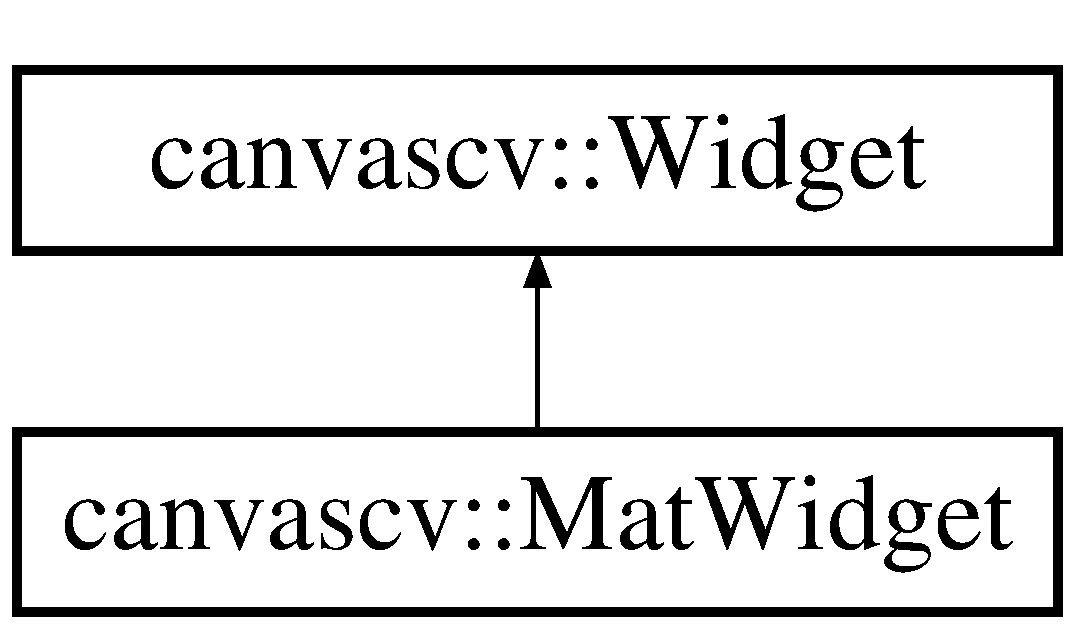
\includegraphics[height=2.000000cm]{classcanvascv_1_1MatWidget}
\end{center}
\end{figure}
\subsection*{Public Member Functions}
\begin{DoxyCompactItemize}
\item 
const cv\+::\+Mat \& \hyperlink{classcanvascv_1_1MatWidget_ae6d1de3cf8ba58584154fa4f5d38dbe6}{get\+Mat} () const \hypertarget{classcanvascv_1_1MatWidget_ae6d1de3cf8ba58584154fa4f5d38dbe6}{}\label{classcanvascv_1_1MatWidget_ae6d1de3cf8ba58584154fa4f5d38dbe6}

\begin{DoxyCompactList}\small\item\em get the FG Mat which is displayed by the widget \end{DoxyCompactList}\item 
void \hyperlink{classcanvascv_1_1MatWidget_af46e7d8f9a6c4a3688f1fad6e5ad351e}{set\+Mat} (const cv\+::\+Mat \&value)
\begin{DoxyCompactList}\small\item\em set\+Mat \end{DoxyCompactList}\item 
virtual const char $\ast$ \hyperlink{classcanvascv_1_1MatWidget_abb3e9e14071456367a4e6717d064f1dd}{get\+Type} () const 
\begin{DoxyCompactList}\small\item\em get\+Type is always implemented by derived to return the same static pointer per widget. \end{DoxyCompactList}\end{DoxyCompactItemize}
\subsection*{Static Public Member Functions}
\begin{DoxyCompactItemize}
\item 
static std\+::shared\+\_\+ptr$<$ \hyperlink{classcanvascv_1_1MatWidget}{Mat\+Widget} $>$ \hyperlink{classcanvascv_1_1MatWidget_aca0ea4c34265c70f59a929968ca64aba}{create} (\hyperlink{classcanvascv_1_1Layout}{Layout} \&layout, cv\+::\+Mat mat=cv\+::\+Mat(), const cv\+::\+Point \&pos=cv\+::\+Point(0, 0))
\begin{DoxyCompactList}\small\item\em create a \hyperlink{classcanvascv_1_1MatWidget}{Mat\+Widget} widget \end{DoxyCompactList}\end{DoxyCompactItemize}
\subsection*{Protected Member Functions}
\begin{DoxyCompactItemize}
\item 
virtual const cv\+::\+Rect \& \hyperlink{classcanvascv_1_1MatWidget_a318736f6602bc2fccc7758be88ca3c4d}{get\+Rect} ()\hypertarget{classcanvascv_1_1MatWidget_a318736f6602bc2fccc7758be88ca3c4d}{}\label{classcanvascv_1_1MatWidget_a318736f6602bc2fccc7758be88ca3c4d}

\begin{DoxyCompactList}\small\item\em Actual size the widget is occupying due to \hyperlink{classcanvascv_1_1Layout}{Layout} manager. \end{DoxyCompactList}\item 
virtual const cv\+::\+Rect \& \hyperlink{classcanvascv_1_1MatWidget_a8348b409495b367b48f297cef4c577c0}{get\+Minimal\+Rect} ()\hypertarget{classcanvascv_1_1MatWidget_a8348b409495b367b48f297cef4c577c0}{}\label{classcanvascv_1_1MatWidget_a8348b409495b367b48f297cef4c577c0}

\begin{DoxyCompactList}\small\item\em Minimal size the widget coould have occupy. \end{DoxyCompactList}\item 
virtual void \hyperlink{classcanvascv_1_1MatWidget_a01c9f938495de6c6d99ef6d41c925c21}{recalc} ()\hypertarget{classcanvascv_1_1MatWidget_a01c9f938495de6c6d99ef6d41c925c21}{}\label{classcanvascv_1_1MatWidget_a01c9f938495de6c6d99ef6d41c925c21}

\begin{DoxyCompactList}\small\item\em update self so next call to \textquotesingle{}draw\textquotesingle{} will display correctly \end{DoxyCompactList}\item 
virtual void \hyperlink{classcanvascv_1_1MatWidget_abea96f3d0ef3407bc63b112624756247}{draw\+FG} (cv\+::\+Mat \&dst)\hypertarget{classcanvascv_1_1MatWidget_abea96f3d0ef3407bc63b112624756247}{}\label{classcanvascv_1_1MatWidget_abea96f3d0ef3407bc63b112624756247}

\begin{DoxyCompactList}\small\item\em dst is the roi of the widget size and not the full image \end{DoxyCompactList}\end{DoxyCompactItemize}
\subsection*{Additional Inherited Members}


\subsection{Detailed Description}
Displaying a Mat on an Open\+CV window, with alpha channel support. 

\subsection{Member Function Documentation}
\index{canvascv\+::\+Mat\+Widget@{canvascv\+::\+Mat\+Widget}!create@{create}}
\index{create@{create}!canvascv\+::\+Mat\+Widget@{canvascv\+::\+Mat\+Widget}}
\subsubsection[{\texorpdfstring{create(\+Layout \&layout, cv\+::\+Mat mat=cv\+::\+Mat(), const cv\+::\+Point \&pos=cv\+::\+Point(0, 0))}{create(Layout &layout, cv::Mat mat=cv::Mat(), const cv::Point &pos=cv::Point(0, 0))}}]{\setlength{\rightskip}{0pt plus 5cm}static std\+::shared\+\_\+ptr$<${\bf Mat\+Widget}$>$ canvascv\+::\+Mat\+Widget\+::create (
\begin{DoxyParamCaption}
\item[{{\bf Layout} \&}]{layout, }
\item[{cv\+::\+Mat}]{mat = {\ttfamily cv\+:\+:Mat()}, }
\item[{const cv\+::\+Point \&}]{pos = {\ttfamily cv\+:\+:Point(0,~0)}}
\end{DoxyParamCaption}
)\hspace{0.3cm}{\ttfamily [static]}}\hypertarget{classcanvascv_1_1MatWidget_aca0ea4c34265c70f59a929968ca64aba}{}\label{classcanvascv_1_1MatWidget_aca0ea4c34265c70f59a929968ca64aba}

\begin{DoxyParams}{Parameters}
{\em layout} & widgets are placed in layouts Canvas/\+V\+Frame/\+H\+Frame/... \\
\hline
{\em mat} & will be referenced by this widget (not copied) \\
\hline
{\em pos} & location in the \hyperlink{classcanvascv_1_1Layout}{Layout} (Layouts can ignore that) \\
\hline
\end{DoxyParams}
\begin{Desc}
\item[Examples\+: ]\par
\hyperlink{example_matwidget_8cpp-example}{example\+\_\+matwidget.\+cpp}.\end{Desc}
\index{canvascv\+::\+Mat\+Widget@{canvascv\+::\+Mat\+Widget}!get\+Type@{get\+Type}}
\index{get\+Type@{get\+Type}!canvascv\+::\+Mat\+Widget@{canvascv\+::\+Mat\+Widget}}
\subsubsection[{\texorpdfstring{get\+Type() const }{getType() const }}]{\setlength{\rightskip}{0pt plus 5cm}virtual const char$\ast$ canvascv\+::\+Mat\+Widget\+::get\+Type (
\begin{DoxyParamCaption}
{}
\end{DoxyParamCaption}
) const\hspace{0.3cm}{\ttfamily [virtual]}}\hypertarget{classcanvascv_1_1MatWidget_abb3e9e14071456367a4e6717d064f1dd}{}\label{classcanvascv_1_1MatWidget_abb3e9e14071456367a4e6717d064f1dd}
\begin{DoxyReturn}{Returns}
const char $\ast$ pointer to string with widget type name 
\end{DoxyReturn}


Implements \hyperlink{classcanvascv_1_1Widget_a85884269bd53ab91203f099a586efa43}{canvascv\+::\+Widget}.

\index{canvascv\+::\+Mat\+Widget@{canvascv\+::\+Mat\+Widget}!set\+Mat@{set\+Mat}}
\index{set\+Mat@{set\+Mat}!canvascv\+::\+Mat\+Widget@{canvascv\+::\+Mat\+Widget}}
\subsubsection[{\texorpdfstring{set\+Mat(const cv\+::\+Mat \&value)}{setMat(const cv::Mat &value)}}]{\setlength{\rightskip}{0pt plus 5cm}void canvascv\+::\+Mat\+Widget\+::set\+Mat (
\begin{DoxyParamCaption}
\item[{const cv\+::\+Mat \&}]{value}
\end{DoxyParamCaption}
)}\hypertarget{classcanvascv_1_1MatWidget_af46e7d8f9a6c4a3688f1fad6e5ad351e}{}\label{classcanvascv_1_1MatWidget_af46e7d8f9a6c4a3688f1fad6e5ad351e}
set the FG Mat which is displayed by the widget 
\begin{DoxyParams}{Parameters}
{\em value} & will assigned (not copied) to an internal Mat \\
\hline
\end{DoxyParams}


The documentation for this class was generated from the following file\+:\begin{DoxyCompactItemize}
\item 
Canvas\+C\+V-\/doxygen/src/canvascv/widgets/matwidget.\+h\end{DoxyCompactItemize}

\hypertarget{classcanvascv_1_1MsgBox}{}\section{canvascv\+:\+:Msg\+Box Class Reference}
\label{classcanvascv_1_1MsgBox}\index{canvascv\+::\+Msg\+Box@{canvascv\+::\+Msg\+Box}}


The \hyperlink{classcanvascv_1_1MsgBox}{Msg\+Box} class.  




{\ttfamily \#include $<$msgbox.\+h$>$}

Inheritance diagram for canvascv\+:\+:Msg\+Box\+:\begin{figure}[H]
\begin{center}
\leavevmode
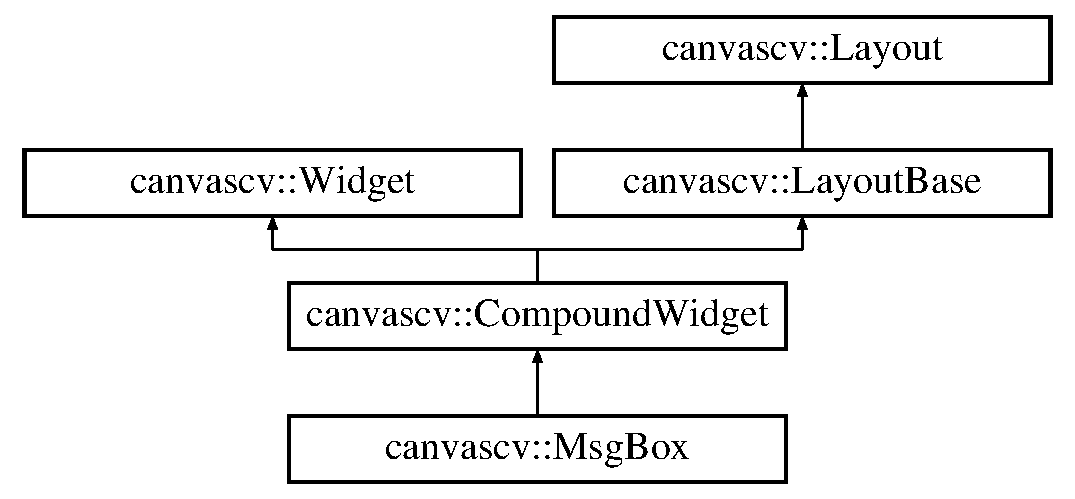
\includegraphics[height=4.000000cm]{classcanvascv_1_1MsgBox}
\end{center}
\end{figure}
\subsection*{Public Member Functions}
\begin{DoxyCompactItemize}
\item 
int \hyperlink{classcanvascv_1_1MsgBox_a8762fe664f293389a1b823c75dc545e1}{get\+User\+Selection} (bool blocking=false)
\begin{DoxyCompactList}\small\item\em get\+User\+Selection \end{DoxyCompactList}\item 
std\+::string \hyperlink{classcanvascv_1_1MsgBox_af97285a26857652a316387505ff7dce0}{get\+Text\+At} (int index) const 
\begin{DoxyCompactList}\small\item\em get\+Text\+At \end{DoxyCompactList}\item 
size\+\_\+t \hyperlink{classcanvascv_1_1MsgBox_adc1e629426ea62ff9b1391c18fcb3a4a}{size} () const \hypertarget{classcanvascv_1_1MsgBox_adc1e629426ea62ff9b1391c18fcb3a4a}{}\label{classcanvascv_1_1MsgBox_adc1e629426ea62ff9b1391c18fcb3a4a}

\begin{DoxyCompactList}\small\item\em return nunmber of buttons \end{DoxyCompactList}\item 
virtual const char $\ast$ \hyperlink{classcanvascv_1_1MsgBox_ad846e38adb000c10fac57e433d894001}{get\+Type} () const 
\begin{DoxyCompactList}\small\item\em get\+Type is always implemented by derived to return the same static pointer per widget. \end{DoxyCompactList}\end{DoxyCompactItemize}
\subsection*{Static Public Member Functions}
\begin{DoxyCompactItemize}
\item 
static std\+::shared\+\_\+ptr$<$ \hyperlink{classcanvascv_1_1MsgBox}{Msg\+Box} $>$ \hyperlink{classcanvascv_1_1MsgBox_a3bf0019e83e367e415da29286db2c5d0}{create} (\hyperlink{classcanvascv_1_1Canvas}{Canvas} \&canvas, const std\+::string \&msg, std\+::vector$<$ std\+::string $>$ button\+Names=\{\char`\"{}Ok\char`\"{}\}, Widget\+::\+C\+B\+User\+Selection cb\+User\+Selection=\hyperlink{classcanvascv_1_1Widget_a977cbd39cf203c5866f07f3645c7e4bc}{Widget\+::\+C\+B\+User\+Selection}(), const cv\+::\+Point \&pos=cv\+::\+Point(-\/1,-\/1))
\begin{DoxyCompactList}\small\item\em create a message box widget which is closed automatically \end{DoxyCompactList}\item 
static int \hyperlink{classcanvascv_1_1MsgBox_a1eb6af15c2393ce6cda9ce277c01d200}{create\+Modal} (const std\+::string \&title, const std\+::string \&msg, std\+::vector$<$ std\+::string $>$ button\+Names=\{\char`\"{}Ok\char`\"{}\}, Widget\+::\+C\+B\+User\+Selection cb\+User\+Selection=\hyperlink{classcanvascv_1_1Widget_a977cbd39cf203c5866f07f3645c7e4bc}{Widget\+::\+C\+B\+User\+Selection}())
\begin{DoxyCompactList}\small\item\em create\+Modal \end{DoxyCompactList}\end{DoxyCompactItemize}
\subsection*{Protected Member Functions}
\begin{DoxyCompactItemize}
\item 
virtual void \hyperlink{classcanvascv_1_1MsgBox_a1eea452acb76e5a5a0588bf83cc91325}{recalc\+Compound} ()
\begin{DoxyCompactList}\small\item\em recalc\+Compound \end{DoxyCompactList}\end{DoxyCompactItemize}
\subsection*{Additional Inherited Members}


\subsection{Detailed Description}
Use a message box with any number of buttons on an Open\+CV window 

\subsection{Member Function Documentation}
\index{canvascv\+::\+Msg\+Box@{canvascv\+::\+Msg\+Box}!create@{create}}
\index{create@{create}!canvascv\+::\+Msg\+Box@{canvascv\+::\+Msg\+Box}}
\subsubsection[{\texorpdfstring{create(\+Canvas \&canvas, const std\+::string \&msg, std\+::vector$<$ std\+::string $>$ button\+Names=\lcurly{}""Ok""\rcurly{}, Widget\+::\+C\+B\+User\+Selection cb\+User\+Selection=\+Widget\+::\+C\+B\+User\+Selection(), const cv\+::\+Point \&pos=cv\+::\+Point(-\/1,-\/1))}{create(Canvas &canvas, const std::string &msg, std::vector< std::string > buttonNames=\{"Ok"\}, Widget::CBUserSelection cbUserSelection=Widget::CBUserSelection(), const cv::Point &pos=cv::Point(-1,-1))}}]{\setlength{\rightskip}{0pt plus 5cm}static std\+::shared\+\_\+ptr$<${\bf Msg\+Box}$>$ canvascv\+::\+Msg\+Box\+::create (
\begin{DoxyParamCaption}
\item[{{\bf Canvas} \&}]{canvas, }
\item[{const std\+::string \&}]{msg, }
\item[{std\+::vector$<$ std\+::string $>$}]{button\+Names = {\ttfamily \{\char`\"{}Ok\char`\"{}\}}, }
\item[{{\bf Widget\+::\+C\+B\+User\+Selection}}]{cb\+User\+Selection = {\ttfamily {\bf Widget\+::\+C\+B\+User\+Selection}()}, }
\item[{const cv\+::\+Point \&}]{pos = {\ttfamily cv\+:\+:Point(-\/1,-\/1)}}
\end{DoxyParamCaption}
)\hspace{0.3cm}{\ttfamily [static]}}\hypertarget{classcanvascv_1_1MsgBox_a3bf0019e83e367e415da29286db2c5d0}{}\label{classcanvascv_1_1MsgBox_a3bf0019e83e367e415da29286db2c5d0}
The \hyperlink{classcanvascv_1_1MsgBox}{Msg\+Box} is not modal -\/ does not block input to other widgets. For a modal \hyperlink{classcanvascv_1_1MsgBox}{Msg\+Box} inside a \hyperlink{classcanvascv_1_1Canvas}{Canvas} use \hyperlink{classcanvascv_1_1MsgBox_a3bf0019e83e367e415da29286db2c5d0}{create()} and get\+User\+Selection(true). 
\begin{DoxyParams}{Parameters}
{\em canvas} & must be a \hyperlink{classcanvascv_1_1Canvas}{Canvas} reference for a \hyperlink{classcanvascv_1_1MsgBox}{Msg\+Box} \\
\hline
{\em msg} & what to display in the \hyperlink{classcanvascv_1_1MsgBox}{Msg\+Box} \\
\hline
{\em button\+Names} & automatically create buttons with names of button\+Names \\
\hline
{\em cb\+User\+Selection} & a callback to invoke with index of pressed button \\
\hline
{\em pos} & location in the \hyperlink{classcanvascv_1_1Canvas}{Canvas} (the default is the center of the \hyperlink{classcanvascv_1_1Canvas}{Canvas}) \\
\hline
\end{DoxyParams}
\begin{DoxyReturn}{Returns}
a smart pointer copy of the object kept in the \hyperlink{classcanvascv_1_1Layout}{Layout} 
\begin{DoxyCode}
Canvas c(winName, image.size());
\textcolor{keyword}{auto} msgBox = \hyperlink{classcanvascv_1_1MsgBox_a3bf0019e83e367e415da29286db2c5d0}{MsgBox::create}(c,
                             \textcolor{stringliteral}{"This is a MsgBox example\(\backslash\)n"}
                             \textcolor{stringliteral}{"with 2 lines"}, \{
                                 \textcolor{stringliteral}{"Ok"},           \textcolor{comment}{// 0}
                                 \textcolor{stringliteral}{"Cancel"},       \textcolor{comment}{// 1}
                                 \textcolor{stringliteral}{"Somthing else"} \textcolor{comment}{// 2}
                             \});

\textcolor{keywordflow}{while}(...)
\{
    \textcolor{keywordflow}{if} (msgBox && msgBox->getUserSelection() != -1)
    \{
        cout << \textcolor{stringliteral}{"MsgBox was pressed with key index "} << msgBox->getUserSelection() << endl;
        msgBox.reset();
    \}
    c.\hyperlink{classcanvascv_1_1Canvas_a018c66e277de7904b8146ea3f3feebdd}{redrawOn}(...);
    imshow(...);
    key = c.\hyperlink{classcanvascv_1_1Canvas_a59397db05f5d9e45264f626f6a2ae528}{waitKeyEx}(...); \textcolor{comment}{// GUI and callbacks happen here}
\}
\end{DoxyCode}
 Or you could use the callback version (see the example) 
\end{DoxyReturn}
\begin{DoxySeeAlso}{See also}
\hyperlink{classcanvascv_1_1MsgBox_a8762fe664f293389a1b823c75dc545e1}{get\+User\+Selection} 
\end{DoxySeeAlso}
\begin{Desc}
\item[Examples\+: ]\par
\hyperlink{example_msgbox_8cpp-example}{example\+\_\+msgbox.\+cpp}.\end{Desc}
\index{canvascv\+::\+Msg\+Box@{canvascv\+::\+Msg\+Box}!create\+Modal@{create\+Modal}}
\index{create\+Modal@{create\+Modal}!canvascv\+::\+Msg\+Box@{canvascv\+::\+Msg\+Box}}
\subsubsection[{\texorpdfstring{create\+Modal(const std\+::string \&title, const std\+::string \&msg, std\+::vector$<$ std\+::string $>$ button\+Names=\lcurly{}""Ok""\rcurly{}, Widget\+::\+C\+B\+User\+Selection cb\+User\+Selection=\+Widget\+::\+C\+B\+User\+Selection())}{createModal(const std::string &title, const std::string &msg, std::vector< std::string > buttonNames=\{"Ok"\}, Widget::CBUserSelection cbUserSelection=Widget::CBUserSelection())}}]{\setlength{\rightskip}{0pt plus 5cm}static int canvascv\+::\+Msg\+Box\+::create\+Modal (
\begin{DoxyParamCaption}
\item[{const std\+::string \&}]{title, }
\item[{const std\+::string \&}]{msg, }
\item[{std\+::vector$<$ std\+::string $>$}]{button\+Names = {\ttfamily \{\char`\"{}Ok\char`\"{}\}}, }
\item[{{\bf Widget\+::\+C\+B\+User\+Selection}}]{cb\+User\+Selection = {\ttfamily {\bf Widget\+::\+C\+B\+User\+Selection}()}}
\end{DoxyParamCaption}
)\hspace{0.3cm}{\ttfamily [static]}}\hypertarget{classcanvascv_1_1MsgBox_a1eb6af15c2393ce6cda9ce277c01d200}{}\label{classcanvascv_1_1MsgBox_a1eb6af15c2393ce6cda9ce277c01d200}
opens a modal (blocking) \hyperlink{classcanvascv_1_1MsgBox}{Msg\+Box} in it\textquotesingle{}s own window and immediatly waits for a user selection. For a modal \hyperlink{classcanvascv_1_1MsgBox}{Msg\+Box} inside a \hyperlink{classcanvascv_1_1Canvas}{Canvas} use \hyperlink{classcanvascv_1_1MsgBox_a3bf0019e83e367e415da29286db2c5d0}{create()} and get\+User\+Selection(true). 
\begin{DoxyParams}{Parameters}
{\em title} & is the title of the new window \\
\hline
{\em msg} & what to display in the \hyperlink{classcanvascv_1_1MsgBox}{Msg\+Box} \\
\hline
{\em button\+Names} & automatically create buttons with names of button\+Names \\
\hline
{\em cb\+User\+Selection} & a callback to invoke with index of pressed button \\
\hline
\end{DoxyParams}
\begin{DoxyReturn}{Returns}
return result of \hyperlink{classcanvascv_1_1MsgBox_a8762fe664f293389a1b823c75dc545e1}{get\+User\+Selection()} 
\end{DoxyReturn}
\begin{DoxySeeAlso}{See also}
get\+User\+Selection(true) 
\end{DoxySeeAlso}
\index{canvascv\+::\+Msg\+Box@{canvascv\+::\+Msg\+Box}!get\+Text\+At@{get\+Text\+At}}
\index{get\+Text\+At@{get\+Text\+At}!canvascv\+::\+Msg\+Box@{canvascv\+::\+Msg\+Box}}
\subsubsection[{\texorpdfstring{get\+Text\+At(int index) const }{getTextAt(int index) const }}]{\setlength{\rightskip}{0pt plus 5cm}std\+::string canvascv\+::\+Msg\+Box\+::get\+Text\+At (
\begin{DoxyParamCaption}
\item[{int}]{index}
\end{DoxyParamCaption}
) const}\hypertarget{classcanvascv_1_1MsgBox_af97285a26857652a316387505ff7dce0}{}\label{classcanvascv_1_1MsgBox_af97285a26857652a316387505ff7dce0}
return the text at index index 
\begin{DoxyParams}{Parameters}
{\em index} & is the index you want the text for \\
\hline
\end{DoxyParams}
\begin{DoxyReturn}{Returns}
return the text at index index or empty string if invalid index 
\end{DoxyReturn}
\index{canvascv\+::\+Msg\+Box@{canvascv\+::\+Msg\+Box}!get\+Type@{get\+Type}}
\index{get\+Type@{get\+Type}!canvascv\+::\+Msg\+Box@{canvascv\+::\+Msg\+Box}}
\subsubsection[{\texorpdfstring{get\+Type() const }{getType() const }}]{\setlength{\rightskip}{0pt plus 5cm}virtual const char$\ast$ canvascv\+::\+Msg\+Box\+::get\+Type (
\begin{DoxyParamCaption}
{}
\end{DoxyParamCaption}
) const\hspace{0.3cm}{\ttfamily [virtual]}}\hypertarget{classcanvascv_1_1MsgBox_ad846e38adb000c10fac57e433d894001}{}\label{classcanvascv_1_1MsgBox_ad846e38adb000c10fac57e433d894001}
\begin{DoxyReturn}{Returns}
const char $\ast$ pointer to string with widget type name 
\end{DoxyReturn}


Implements \hyperlink{classcanvascv_1_1Widget_a85884269bd53ab91203f099a586efa43}{canvascv\+::\+Widget}.

\index{canvascv\+::\+Msg\+Box@{canvascv\+::\+Msg\+Box}!get\+User\+Selection@{get\+User\+Selection}}
\index{get\+User\+Selection@{get\+User\+Selection}!canvascv\+::\+Msg\+Box@{canvascv\+::\+Msg\+Box}}
\subsubsection[{\texorpdfstring{get\+User\+Selection(bool blocking=false)}{getUserSelection(bool blocking=false)}}]{\setlength{\rightskip}{0pt plus 5cm}int canvascv\+::\+Msg\+Box\+::get\+User\+Selection (
\begin{DoxyParamCaption}
\item[{bool}]{blocking = {\ttfamily false}}
\end{DoxyParamCaption}
)}\hypertarget{classcanvascv_1_1MsgBox_a8762fe664f293389a1b823c75dc545e1}{}\label{classcanvascv_1_1MsgBox_a8762fe664f293389a1b823c75dc545e1}
get what the user pressed 
\begin{DoxyParams}{Parameters}
{\em blocking} & if true, block waiting on the \hyperlink{classcanvascv_1_1MsgBox}{Msg\+Box} until a button is pressed \\
\hline
\end{DoxyParams}
\begin{DoxyReturn}{Returns}
returns pressed button index or -\/1 if not pressed 
\end{DoxyReturn}
\index{canvascv\+::\+Msg\+Box@{canvascv\+::\+Msg\+Box}!recalc\+Compound@{recalc\+Compound}}
\index{recalc\+Compound@{recalc\+Compound}!canvascv\+::\+Msg\+Box@{canvascv\+::\+Msg\+Box}}
\subsubsection[{\texorpdfstring{recalc\+Compound()}{recalcCompound()}}]{\setlength{\rightskip}{0pt plus 5cm}virtual void canvascv\+::\+Msg\+Box\+::recalc\+Compound (
\begin{DoxyParamCaption}
{}
\end{DoxyParamCaption}
)\hspace{0.3cm}{\ttfamily [protected]}, {\ttfamily [virtual]}}\hypertarget{classcanvascv_1_1MsgBox_a1eea452acb76e5a5a0588bf83cc91325}{}\label{classcanvascv_1_1MsgBox_a1eea452acb76e5a5a0588bf83cc91325}
Your BG size recalculation/allocation and FG drawing is done here. It is done semi automatically. Is you invoke setters in this method on your internal widgets, then make sure to update them and/or their layout 

Implements \hyperlink{classcanvascv_1_1CompoundWidget_a4a4f8241d6fd187ffcae2c7968f13864}{canvascv\+::\+Compound\+Widget}.



The documentation for this class was generated from the following file\+:\begin{DoxyCompactItemize}
\item 
Canvas\+C\+V-\/doxygen/src/canvascv/widgets/msgbox.\+h\end{DoxyCompactItemize}

\hypertarget{classcanvascv_1_1Polygon}{}\section{canvascv\+:\+:Polygon Class Reference}
\label{classcanvascv_1_1Polygon}\index{canvascv\+::\+Polygon@{canvascv\+::\+Polygon}}


The \hyperlink{classcanvascv_1_1Polygon}{Polygon} class.  




{\ttfamily \#include $<$polygon.\+h$>$}

Inheritance diagram for canvascv\+:\+:Polygon\+:\begin{figure}[H]
\begin{center}
\leavevmode
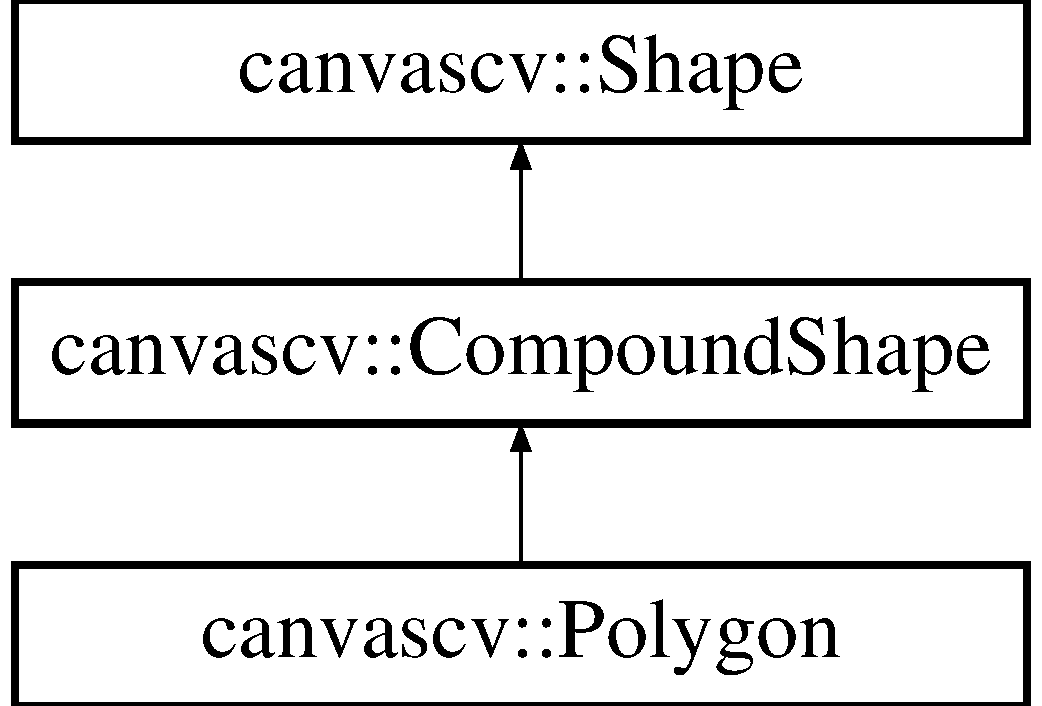
\includegraphics[height=3.000000cm]{classcanvascv_1_1Polygon}
\end{center}
\end{figure}
\subsection*{Public Member Functions}
\begin{DoxyCompactItemize}
\item 
bool \hyperlink{classcanvascv_1_1Polygon_a974ef1dbfb5314bd4c60fa07bf318b54}{is\+Point\+In\+Poly} (const cv\+::\+Point \&pos) const \hypertarget{classcanvascv_1_1Polygon_a974ef1dbfb5314bd4c60fa07bf318b54}{}\label{classcanvascv_1_1Polygon_a974ef1dbfb5314bd4c60fa07bf318b54}

\begin{DoxyCompactList}\small\item\em returns true if pos is in the polygon \end{DoxyCompactList}\item 
{\footnotesize template$<$typename \+\_\+\+TP $>$ }\\void \hyperlink{classcanvascv_1_1Polygon_ada0df457225c06769d7a90d71f58ed7f}{get\+Points} (vector$<$ Point\+\_\+$<$ \+\_\+\+TP $>$$>$ \&out)
\begin{DoxyCompactList}\small\item\em get\+Points \end{DoxyCompactList}\item 
virtual bool \hyperlink{classcanvascv_1_1Polygon_a9934b8f096b4eba4580f6bd0ce0a4ab9}{is\+At\+Pos} (const cv\+::\+Point \&pos)\hypertarget{classcanvascv_1_1Polygon_a9934b8f096b4eba4580f6bd0ce0a4ab9}{}\label{classcanvascv_1_1Polygon_a9934b8f096b4eba4580f6bd0ce0a4ab9}

\begin{DoxyCompactList}\small\item\em returns true if shape is at pos, false otherwise \end{DoxyCompactList}\item 
virtual std\+::list$<$ \hyperlink{classcanvascv_1_1Handle}{Handle} $\ast$ $>$ \hyperlink{classcanvascv_1_1Polygon_a4e15fc33d4dceb99e4f063b5dda2e658}{get\+Connection\+Targets} ()
\begin{DoxyCompactList}\small\item\em get\+Connection\+Targets \end{DoxyCompactList}\item 
virtual bool \hyperlink{classcanvascv_1_1Polygon_aca22b914de1ced559faf4fd5426073ff}{key\+Pressed} (int \&key)
\begin{DoxyCompactList}\small\item\em key\+Pressed will be called by \hyperlink{classcanvascv_1_1Canvas}{Canvas} for active shapes \end{DoxyCompactList}\item 
virtual const char $\ast$ \hyperlink{classcanvascv_1_1Polygon_a58dab27bcdfcaab026e0e79157e68318}{get\+Type} () const 
\begin{DoxyCompactList}\small\item\em get\+Type is always implemented by derived to return the same static pointer per shape. \end{DoxyCompactList}\end{DoxyCompactItemize}
\subsection*{Protected Member Functions}
\begin{DoxyCompactItemize}
\item 
virtual void \hyperlink{classcanvascv_1_1Polygon_a32e073cb9579fdf4645daf14e5143f22}{draw} (cv\+::\+Mat \&canvas)
\begin{DoxyCompactList}\small\item\em draw shape on the canvas \end{DoxyCompactList}\item 
virtual bool \hyperlink{classcanvascv_1_1Polygon_a87ce20dbc22fd0ce39d6e81de5e515ae}{mouse\+Pressed} (const cv\+::\+Point \&pos, bool on\+Create=false)
\begin{DoxyCompactList}\small\item\em mouse\+Pressed \end{DoxyCompactList}\item 
virtual bool \hyperlink{classcanvascv_1_1Polygon_aacc442ef4c0438ddb78c6ccce8e86618}{mouse\+Moved} (const cv\+::\+Point \&pos)
\begin{DoxyCompactList}\small\item\em mouse\+Moved \end{DoxyCompactList}\item 
virtual bool \hyperlink{classcanvascv_1_1Polygon_afea6bbe1beef916e6ec47ed257cb2374}{mouse\+Released} (const cv\+::\+Point \&pos)
\begin{DoxyCompactList}\small\item\em mouse\+Released \end{DoxyCompactList}\item 
virtual void \hyperlink{classcanvascv_1_1Polygon_a9cc78c0ace7940aa2cd78245b63938bc}{lost\+Focus} ()\hypertarget{classcanvascv_1_1Polygon_a9cc78c0ace7940aa2cd78245b63938bc}{}\label{classcanvascv_1_1Polygon_a9cc78c0ace7940aa2cd78245b63938bc}

\begin{DoxyCompactList}\small\item\em lost\+Focus is called by \hyperlink{classcanvascv_1_1Canvas}{Canvas} if we\textquotesingle{}re in it and just became non-\/active \end{DoxyCompactList}\end{DoxyCompactItemize}
\subsection*{Additional Inherited Members}


\subsection{Detailed Description}
Allows you to draw a polygon by mouse or from code \begin{DoxySeeAlso}{See also}

\end{DoxySeeAlso}


\subsection{Member Function Documentation}
\index{canvascv\+::\+Polygon@{canvascv\+::\+Polygon}!draw@{draw}}
\index{draw@{draw}!canvascv\+::\+Polygon@{canvascv\+::\+Polygon}}
\subsubsection[{\texorpdfstring{draw(cv\+::\+Mat \&canvas)}{draw(cv::Mat &canvas)}}]{\setlength{\rightskip}{0pt plus 5cm}virtual void canvascv\+::\+Polygon\+::draw (
\begin{DoxyParamCaption}
\item[{cv\+::\+Mat \&}]{canvas}
\end{DoxyParamCaption}
)\hspace{0.3cm}{\ttfamily [protected]}, {\ttfamily [virtual]}}\hypertarget{classcanvascv_1_1Polygon_a32e073cb9579fdf4645daf14e5143f22}{}\label{classcanvascv_1_1Polygon_a32e073cb9579fdf4645daf14e5143f22}

\begin{DoxyParams}{Parameters}
{\em canvas} & \\
\hline
\end{DoxyParams}


Reimplemented from \hyperlink{classcanvascv_1_1CompoundShape_a6ec60ee0340ed25274e3ac1349345953}{canvascv\+::\+Compound\+Shape}.

\index{canvascv\+::\+Polygon@{canvascv\+::\+Polygon}!get\+Connection\+Targets@{get\+Connection\+Targets}}
\index{get\+Connection\+Targets@{get\+Connection\+Targets}!canvascv\+::\+Polygon@{canvascv\+::\+Polygon}}
\subsubsection[{\texorpdfstring{get\+Connection\+Targets()}{getConnectionTargets()}}]{\setlength{\rightskip}{0pt plus 5cm}virtual std\+::list$<${\bf Handle} $\ast$$>$ canvascv\+::\+Polygon\+::get\+Connection\+Targets (
\begin{DoxyParamCaption}
{}
\end{DoxyParamCaption}
)\hspace{0.3cm}{\ttfamily [virtual]}}\hypertarget{classcanvascv_1_1Polygon_a4e15fc33d4dceb99e4f063b5dda2e658}{}\label{classcanvascv_1_1Polygon_a4e15fc33d4dceb99e4f063b5dda2e658}
Return a list of Handles this shape allows to connect to from other shapes (mainly for \hyperlink{classcanvascv_1_1ShapesConnector}{Shapes\+Connector}) \begin{DoxyReturn}{Returns}
list of \hyperlink{classcanvascv_1_1Handle}{Handle} pointers we \hyperlink{classcanvascv_1_1ShapesConnector}{Shapes\+Connector} can use to connect 
\end{DoxyReturn}


Implements \hyperlink{classcanvascv_1_1Shape_a827822e17e24118e16fa932ac0e71cd2}{canvascv\+::\+Shape}.

\index{canvascv\+::\+Polygon@{canvascv\+::\+Polygon}!get\+Points@{get\+Points}}
\index{get\+Points@{get\+Points}!canvascv\+::\+Polygon@{canvascv\+::\+Polygon}}
\subsubsection[{\texorpdfstring{get\+Points(vector$<$ Point\+\_\+$<$ \+\_\+\+T\+P $>$$>$ \&out)}{getPoints(vector< Point_< _TP >> &out)}}]{\setlength{\rightskip}{0pt plus 5cm}template$<$typename \+\_\+\+TP $>$ void canvascv\+::\+Polygon\+::get\+Points (
\begin{DoxyParamCaption}
\item[{vector$<$ Point\+\_\+$<$ \+\_\+\+TP $>$$>$ \&}]{out}
\end{DoxyParamCaption}
)}\hypertarget{classcanvascv_1_1Polygon_ada0df457225c06769d7a90d71f58ed7f}{}\label{classcanvascv_1_1Polygon_ada0df457225c06769d7a90d71f58ed7f}
return the vertices of the polygon 
\begin{DoxyParams}{Parameters}
{\em out} & will contain the vertices on return \\
\hline
\end{DoxyParams}
\index{canvascv\+::\+Polygon@{canvascv\+::\+Polygon}!get\+Type@{get\+Type}}
\index{get\+Type@{get\+Type}!canvascv\+::\+Polygon@{canvascv\+::\+Polygon}}
\subsubsection[{\texorpdfstring{get\+Type() const }{getType() const }}]{\setlength{\rightskip}{0pt plus 5cm}virtual const char$\ast$ canvascv\+::\+Polygon\+::get\+Type (
\begin{DoxyParamCaption}
{}
\end{DoxyParamCaption}
) const\hspace{0.3cm}{\ttfamily [virtual]}}\hypertarget{classcanvascv_1_1Polygon_a58dab27bcdfcaab026e0e79157e68318}{}\label{classcanvascv_1_1Polygon_a58dab27bcdfcaab026e0e79157e68318}
\begin{DoxyReturn}{Returns}
const char $\ast$ pointer to string with shape type name 
\end{DoxyReturn}


Implements \hyperlink{classcanvascv_1_1Shape_adee3cc696c7e82b0d2946e7e667ddd46}{canvascv\+::\+Shape}.

\index{canvascv\+::\+Polygon@{canvascv\+::\+Polygon}!key\+Pressed@{key\+Pressed}}
\index{key\+Pressed@{key\+Pressed}!canvascv\+::\+Polygon@{canvascv\+::\+Polygon}}
\subsubsection[{\texorpdfstring{key\+Pressed(int \&key)}{keyPressed(int &key)}}]{\setlength{\rightskip}{0pt plus 5cm}virtual bool canvascv\+::\+Polygon\+::key\+Pressed (
\begin{DoxyParamCaption}
\item[{int \&}]{key}
\end{DoxyParamCaption}
)\hspace{0.3cm}{\ttfamily [virtual]}}\hypertarget{classcanvascv_1_1Polygon_aca22b914de1ced559faf4fd5426073ff}{}\label{classcanvascv_1_1Polygon_aca22b914de1ced559faf4fd5426073ff}

\begin{DoxyParams}{Parameters}
{\em key} & was pressed. You must set it to -\/1 if you consumed it. \\
\hline
\end{DoxyParams}
\begin{DoxyReturn}{Returns}
true if we want to stay in focus and false otherwise 
\end{DoxyReturn}


Reimplemented from \hyperlink{classcanvascv_1_1CompoundShape_ac739f68737099c6f5c6d2c70196cd07b}{canvascv\+::\+Compound\+Shape}.

\index{canvascv\+::\+Polygon@{canvascv\+::\+Polygon}!mouse\+Moved@{mouse\+Moved}}
\index{mouse\+Moved@{mouse\+Moved}!canvascv\+::\+Polygon@{canvascv\+::\+Polygon}}
\subsubsection[{\texorpdfstring{mouse\+Moved(const cv\+::\+Point \&pos)}{mouseMoved(const cv::Point &pos)}}]{\setlength{\rightskip}{0pt plus 5cm}virtual bool canvascv\+::\+Polygon\+::mouse\+Moved (
\begin{DoxyParamCaption}
\item[{const cv\+::\+Point \&}]{pos}
\end{DoxyParamCaption}
)\hspace{0.3cm}{\ttfamily [protected]}, {\ttfamily [virtual]}}\hypertarget{classcanvascv_1_1Polygon_aacc442ef4c0438ddb78c6ccce8e86618}{}\label{classcanvascv_1_1Polygon_aacc442ef4c0438ddb78c6ccce8e86618}

\begin{DoxyEnumerate}
\item Was a mouse moved over this shape?
\item If shape is during edit, then these are the mouse position. 
\begin{DoxyParams}{Parameters}
{\em pos} & \\
\hline
\end{DoxyParams}
\begin{DoxyReturn}{Returns}
true if a mouse moved over this shape, or it is during edit. false otherwise. 
\end{DoxyReturn}

\end{DoxyEnumerate}

Reimplemented from \hyperlink{classcanvascv_1_1CompoundShape_a387d1705b99d2053306ffd8d8e67b63b}{canvascv\+::\+Compound\+Shape}.

\index{canvascv\+::\+Polygon@{canvascv\+::\+Polygon}!mouse\+Pressed@{mouse\+Pressed}}
\index{mouse\+Pressed@{mouse\+Pressed}!canvascv\+::\+Polygon@{canvascv\+::\+Polygon}}
\subsubsection[{\texorpdfstring{mouse\+Pressed(const cv\+::\+Point \&pos, bool on\+Create=false)}{mousePressed(const cv::Point &pos, bool onCreate=false)}}]{\setlength{\rightskip}{0pt plus 5cm}virtual bool canvascv\+::\+Polygon\+::mouse\+Pressed (
\begin{DoxyParamCaption}
\item[{const cv\+::\+Point \&}]{pos, }
\item[{bool}]{on\+Create = {\ttfamily false}}
\end{DoxyParamCaption}
)\hspace{0.3cm}{\ttfamily [protected]}, {\ttfamily [virtual]}}\hypertarget{classcanvascv_1_1Polygon_a87ce20dbc22fd0ce39d6e81de5e515ae}{}\label{classcanvascv_1_1Polygon_a87ce20dbc22fd0ce39d6e81de5e515ae}

\begin{DoxyParams}{Parameters}
{\em pos} & \\
\hline
{\em on\+Create} & is true if this is the mouse press which cerated this shape \\
\hline
\end{DoxyParams}
\begin{DoxyReturn}{Returns}
true for keep in focus, false for leave focus 
\end{DoxyReturn}


Reimplemented from \hyperlink{classcanvascv_1_1CompoundShape_a821d046dceaba47114385d1c87e197ce}{canvascv\+::\+Compound\+Shape}.

\index{canvascv\+::\+Polygon@{canvascv\+::\+Polygon}!mouse\+Released@{mouse\+Released}}
\index{mouse\+Released@{mouse\+Released}!canvascv\+::\+Polygon@{canvascv\+::\+Polygon}}
\subsubsection[{\texorpdfstring{mouse\+Released(const cv\+::\+Point \&pos)}{mouseReleased(const cv::Point &pos)}}]{\setlength{\rightskip}{0pt plus 5cm}virtual bool canvascv\+::\+Polygon\+::mouse\+Released (
\begin{DoxyParamCaption}
\item[{const cv\+::\+Point \&}]{pos}
\end{DoxyParamCaption}
)\hspace{0.3cm}{\ttfamily [protected]}, {\ttfamily [virtual]}}\hypertarget{classcanvascv_1_1Polygon_afea6bbe1beef916e6ec47ed257cb2374}{}\label{classcanvascv_1_1Polygon_afea6bbe1beef916e6ec47ed257cb2374}

\begin{DoxyParams}{Parameters}
{\em pos} & \\
\hline
\end{DoxyParams}
\begin{DoxyReturn}{Returns}
true for keep in focus, false for leave focus 
\end{DoxyReturn}


Reimplemented from \hyperlink{classcanvascv_1_1CompoundShape_a01cf027fd5f7ec96525949d0c8ae08a1}{canvascv\+::\+Compound\+Shape}.



The documentation for this class was generated from the following file\+:\begin{DoxyCompactItemize}
\item 
Canvas\+C\+V-\/doxygen/src/canvascv/shapes/polygon.\+h\end{DoxyCompactItemize}

\hypertarget{classcanvascv_1_1RadioButtons}{}\section{canvascv\+:\+:Radio\+Buttons Class Reference}
\label{classcanvascv_1_1RadioButtons}\index{canvascv\+::\+Radio\+Buttons@{canvascv\+::\+Radio\+Buttons}}


The \hyperlink{classcanvascv_1_1RadioButtons}{Radio\+Buttons} class.  




{\ttfamily \#include $<$radiobuttons.\+h$>$}

Inheritance diagram for canvascv\+:\+:Radio\+Buttons\+:\begin{figure}[H]
\begin{center}
\leavevmode
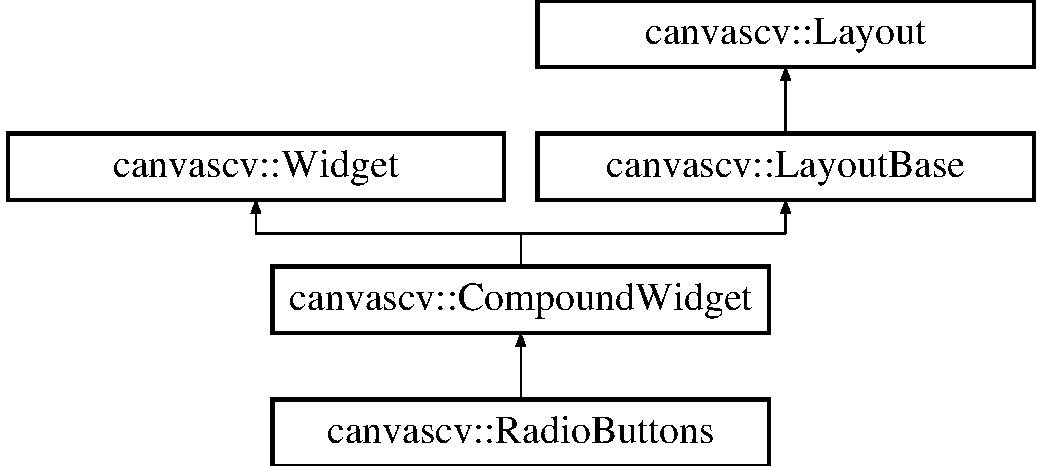
\includegraphics[height=4.000000cm]{classcanvascv_1_1RadioButtons}
\end{center}
\end{figure}
\subsection*{Public Member Functions}
\begin{DoxyCompactItemize}
\item 
void \hyperlink{classcanvascv_1_1RadioButtons_ae5da98c26e7e21d48201b2df06aeb9a3}{set\+Selection} (int value)
\begin{DoxyCompactList}\small\item\em set\+Selection \end{DoxyCompactList}\item 
int \hyperlink{classcanvascv_1_1RadioButtons_ae561b067a70c9e37ebf45befd62f842b}{get\+Selection} () const \hypertarget{classcanvascv_1_1RadioButtons_ae561b067a70c9e37ebf45befd62f842b}{}\label{classcanvascv_1_1RadioButtons_ae561b067a70c9e37ebf45befd62f842b}

\begin{DoxyCompactList}\small\item\em get the current selected option \end{DoxyCompactList}\item 
std\+::string \hyperlink{classcanvascv_1_1RadioButtons_a6a1570cb5b8328fba59bb0c17f63debc}{get\+Text\+At} (int index) const 
\begin{DoxyCompactList}\small\item\em get\+Text\+At \end{DoxyCompactList}\item 
size\+\_\+t \hyperlink{classcanvascv_1_1RadioButtons_a1763254613887741727490ec65c21399}{size} () const \hypertarget{classcanvascv_1_1RadioButtons_a1763254613887741727490ec65c21399}{}\label{classcanvascv_1_1RadioButtons_a1763254613887741727490ec65c21399}

\begin{DoxyCompactList}\small\item\em return nunmber of check boxes in group \end{DoxyCompactList}\item 
void \hyperlink{classcanvascv_1_1RadioButtons_abc50e587c83543df58d8cedcab44daaf}{set\+User\+CB} (\hyperlink{classcanvascv_1_1Widget_a977cbd39cf203c5866f07f3645c7e4bc}{Widget\+::\+C\+B\+User\+Selection} cb\+User\+Selection)\hypertarget{classcanvascv_1_1RadioButtons_abc50e587c83543df58d8cedcab44daaf}{}\label{classcanvascv_1_1RadioButtons_abc50e587c83543df58d8cedcab44daaf}

\begin{DoxyCompactList}\small\item\em cb\+User\+Selection will be invoked per user selection \end{DoxyCompactList}\item 
virtual const char $\ast$ \hyperlink{classcanvascv_1_1RadioButtons_ab62b0f2908eebb4881844bfc25f6319f}{get\+Type} () const 
\begin{DoxyCompactList}\small\item\em get\+Type is always implemented by derived to return the same static pointer per widget. \end{DoxyCompactList}\end{DoxyCompactItemize}
\subsection*{Static Public Member Functions}
\begin{DoxyCompactItemize}
\item 
static std\+::shared\+\_\+ptr$<$ \hyperlink{classcanvascv_1_1RadioButtons}{Radio\+Buttons} $>$ \hyperlink{classcanvascv_1_1RadioButtons_a302902d397822611546929f214604183}{create} (\hyperlink{classcanvascv_1_1Layout}{Layout} \&layout\+Val, std\+::vector$<$ std\+::string $>$ button\+Names, int default\+Selection=-\/1, \hyperlink{classcanvascv_1_1Widget_a977cbd39cf203c5866f07f3645c7e4bc}{Widget\+::\+C\+B\+User\+Selection} cb\+User\+Selection=\hyperlink{classcanvascv_1_1Widget_a977cbd39cf203c5866f07f3645c7e4bc}{Widget\+::\+C\+B\+User\+Selection}(), const cv\+::\+Point \&pos=cv\+::\+Point(0, 0))
\begin{DoxyCompactList}\small\item\em create a radio buttons widget \end{DoxyCompactList}\end{DoxyCompactItemize}
\subsection*{Protected Member Functions}
\begin{DoxyCompactItemize}
\item 
virtual void \hyperlink{classcanvascv_1_1RadioButtons_af4f863f492ca723a0ddac03139a1f187}{recalc\+Compound} ()
\begin{DoxyCompactList}\small\item\em recalc\+Compound \end{DoxyCompactList}\end{DoxyCompactItemize}
\subsection*{Additional Inherited Members}


\subsection{Detailed Description}
Use a radio buttons to get a user selection for multiple options \begin{Desc}
\item[Examples\+: ]\par
\hyperlink{example_add_theme_8cpp-example}{example\+\_\+add\+\_\+theme.\+cpp}, and \hyperlink{example_radiobuttons_8cpp-example}{example\+\_\+radiobuttons.\+cpp}.\end{Desc}


\subsection{Member Function Documentation}
\index{canvascv\+::\+Radio\+Buttons@{canvascv\+::\+Radio\+Buttons}!create@{create}}
\index{create@{create}!canvascv\+::\+Radio\+Buttons@{canvascv\+::\+Radio\+Buttons}}
\subsubsection[{\texorpdfstring{create(\+Layout \&layout\+Val, std\+::vector$<$ std\+::string $>$ button\+Names, int default\+Selection=-\/1, Widget\+::\+C\+B\+User\+Selection cb\+User\+Selection=\+Widget\+::\+C\+B\+User\+Selection(), const cv\+::\+Point \&pos=cv\+::\+Point(0, 0))}{create(Layout &layoutVal, std::vector< std::string > buttonNames, int defaultSelection=-1, Widget::CBUserSelection cbUserSelection=Widget::CBUserSelection(), const cv::Point &pos=cv::Point(0, 0))}}]{\setlength{\rightskip}{0pt plus 5cm}static std\+::shared\+\_\+ptr$<${\bf Radio\+Buttons}$>$ canvascv\+::\+Radio\+Buttons\+::create (
\begin{DoxyParamCaption}
\item[{{\bf Layout} \&}]{layout\+Val, }
\item[{std\+::vector$<$ std\+::string $>$}]{button\+Names, }
\item[{int}]{default\+Selection = {\ttfamily -\/1}, }
\item[{{\bf Widget\+::\+C\+B\+User\+Selection}}]{cb\+User\+Selection = {\ttfamily {\bf Widget\+::\+C\+B\+User\+Selection}()}, }
\item[{const cv\+::\+Point \&}]{pos = {\ttfamily cv\+:\+:Point(0,~0)}}
\end{DoxyParamCaption}
)\hspace{0.3cm}{\ttfamily [static]}}\hypertarget{classcanvascv_1_1RadioButtons_a302902d397822611546929f214604183}{}\label{classcanvascv_1_1RadioButtons_a302902d397822611546929f214604183}

\begin{DoxyParams}{Parameters}
{\em layout\+Val} & widgets are placed in layouts Canvas/\+V\+Frame/\+H\+Frame/... \\
\hline
{\em button\+Names} & automatically create items with names of button\+Names \\
\hline
{\em default\+Selection} & is the index to show as selected on start \\
\hline
{\em cb\+User\+Selection} & a callback to invoke with index of pressed button \\
\hline
{\em pos} & location in the \hyperlink{classcanvascv_1_1Layout}{Layout} (if the layout supports Point locations) \\
\hline
\end{DoxyParams}
\begin{DoxyReturn}{Returns}
a smart pointer copy of the object kept in the \hyperlink{classcanvascv_1_1Layout}{Layout} 
\begin{DoxyCode}
Canvas c(winName, image.size());
\textcolor{keyword}{auto} selectionBox = \hyperlink{classcanvascv_1_1RadioButtons_a302902d397822611546929f214604183}{RadioButtons::create}(c, \{
                                        \textcolor{stringliteral}{"Long Option1"},     \textcolor{comment}{// index 0}
                                        \textcolor{stringliteral}{"Option2\(\backslash\)n2 lines"}, \textcolor{comment}{// index 1}
                                        \textcolor{stringliteral}{"Option3"}           \textcolor{comment}{// index 2}
                                    \},
                                    [](Widget *w, \textcolor{keywordtype}{int} i) \{
    w->setVisible(\textcolor{keyword}{false});
    cout << \textcolor{stringliteral}{"Option "} << i << \textcolor{stringliteral}{" was chosen"} << endl;
\});
\textcolor{keywordflow}{while}(...)
\{
    c.\hyperlink{classcanvascv_1_1Canvas_a018c66e277de7904b8146ea3f3feebdd}{redrawOn}(...);
    imshow(...);
    key = c.\hyperlink{classcanvascv_1_1Canvas_a59397db05f5d9e45264f626f6a2ae528}{waitKeyEx}(...); \textcolor{comment}{// GUI and callbacks happen here}
\}
\end{DoxyCode}
 
\end{DoxyReturn}
\begin{Desc}
\item[Examples\+: ]\par
\hyperlink{example_radiobuttons_8cpp-example}{example\+\_\+radiobuttons.\+cpp}.\end{Desc}
\index{canvascv\+::\+Radio\+Buttons@{canvascv\+::\+Radio\+Buttons}!get\+Text\+At@{get\+Text\+At}}
\index{get\+Text\+At@{get\+Text\+At}!canvascv\+::\+Radio\+Buttons@{canvascv\+::\+Radio\+Buttons}}
\subsubsection[{\texorpdfstring{get\+Text\+At(int index) const }{getTextAt(int index) const }}]{\setlength{\rightskip}{0pt plus 5cm}std\+::string canvascv\+::\+Radio\+Buttons\+::get\+Text\+At (
\begin{DoxyParamCaption}
\item[{int}]{index}
\end{DoxyParamCaption}
) const}\hypertarget{classcanvascv_1_1RadioButtons_a6a1570cb5b8328fba59bb0c17f63debc}{}\label{classcanvascv_1_1RadioButtons_a6a1570cb5b8328fba59bb0c17f63debc}
return the text at index index 
\begin{DoxyParams}{Parameters}
{\em index} & is the index you want the text for \\
\hline
\end{DoxyParams}
\begin{DoxyReturn}{Returns}
return the text at index index or empty string if invalid index 
\end{DoxyReturn}
\begin{Desc}
\item[Examples\+: ]\par
\hyperlink{example_add_theme_8cpp-example}{example\+\_\+add\+\_\+theme.\+cpp}, and \hyperlink{example_radiobuttons_8cpp-example}{example\+\_\+radiobuttons.\+cpp}.\end{Desc}
\index{canvascv\+::\+Radio\+Buttons@{canvascv\+::\+Radio\+Buttons}!get\+Type@{get\+Type}}
\index{get\+Type@{get\+Type}!canvascv\+::\+Radio\+Buttons@{canvascv\+::\+Radio\+Buttons}}
\subsubsection[{\texorpdfstring{get\+Type() const }{getType() const }}]{\setlength{\rightskip}{0pt plus 5cm}virtual const char$\ast$ canvascv\+::\+Radio\+Buttons\+::get\+Type (
\begin{DoxyParamCaption}
{}
\end{DoxyParamCaption}
) const\hspace{0.3cm}{\ttfamily [virtual]}}\hypertarget{classcanvascv_1_1RadioButtons_ab62b0f2908eebb4881844bfc25f6319f}{}\label{classcanvascv_1_1RadioButtons_ab62b0f2908eebb4881844bfc25f6319f}
\begin{DoxyReturn}{Returns}
const char $\ast$ pointer to string with widget type name 
\end{DoxyReturn}


Implements \hyperlink{classcanvascv_1_1Widget_a85884269bd53ab91203f099a586efa43}{canvascv\+::\+Widget}.

\index{canvascv\+::\+Radio\+Buttons@{canvascv\+::\+Radio\+Buttons}!recalc\+Compound@{recalc\+Compound}}
\index{recalc\+Compound@{recalc\+Compound}!canvascv\+::\+Radio\+Buttons@{canvascv\+::\+Radio\+Buttons}}
\subsubsection[{\texorpdfstring{recalc\+Compound()}{recalcCompound()}}]{\setlength{\rightskip}{0pt plus 5cm}virtual void canvascv\+::\+Radio\+Buttons\+::recalc\+Compound (
\begin{DoxyParamCaption}
{}
\end{DoxyParamCaption}
)\hspace{0.3cm}{\ttfamily [protected]}, {\ttfamily [virtual]}}\hypertarget{classcanvascv_1_1RadioButtons_af4f863f492ca723a0ddac03139a1f187}{}\label{classcanvascv_1_1RadioButtons_af4f863f492ca723a0ddac03139a1f187}
Your BG size recalculation/allocation and FG drawing is done here. It is done semi automatically. Is you invoke setters in this method on your internal widgets, then make sure to update them and/or their layout 

Implements \hyperlink{classcanvascv_1_1CompoundWidget_a4a4f8241d6fd187ffcae2c7968f13864}{canvascv\+::\+Compound\+Widget}.

\index{canvascv\+::\+Radio\+Buttons@{canvascv\+::\+Radio\+Buttons}!set\+Selection@{set\+Selection}}
\index{set\+Selection@{set\+Selection}!canvascv\+::\+Radio\+Buttons@{canvascv\+::\+Radio\+Buttons}}
\subsubsection[{\texorpdfstring{set\+Selection(int value)}{setSelection(int value)}}]{\setlength{\rightskip}{0pt plus 5cm}void canvascv\+::\+Radio\+Buttons\+::set\+Selection (
\begin{DoxyParamCaption}
\item[{int}]{value}
\end{DoxyParamCaption}
)}\hypertarget{classcanvascv_1_1RadioButtons_ae5da98c26e7e21d48201b2df06aeb9a3}{}\label{classcanvascv_1_1RadioButtons_ae5da98c26e7e21d48201b2df06aeb9a3}
make a certain option selected 
\begin{DoxyParams}{Parameters}
{\em value} & will be shown as selected \\
\hline
\end{DoxyParams}


The documentation for this class was generated from the following file\+:\begin{DoxyCompactItemize}
\item 
Canvas\+C\+V-\/doxygen/src/canvascv/widgets/radiobuttons.\+h\end{DoxyCompactItemize}

\hypertarget{classcanvascv_1_1Rectangle}{}\section{canvascv\+:\+:Rectangle Class Reference}
\label{classcanvascv_1_1Rectangle}\index{canvascv\+::\+Rectangle@{canvascv\+::\+Rectangle}}


The \hyperlink{classcanvascv_1_1Rectangle}{Rectangle} class.  




{\ttfamily \#include $<$rectangle.\+h$>$}

Inheritance diagram for canvascv\+:\+:Rectangle\+:\begin{figure}[H]
\begin{center}
\leavevmode
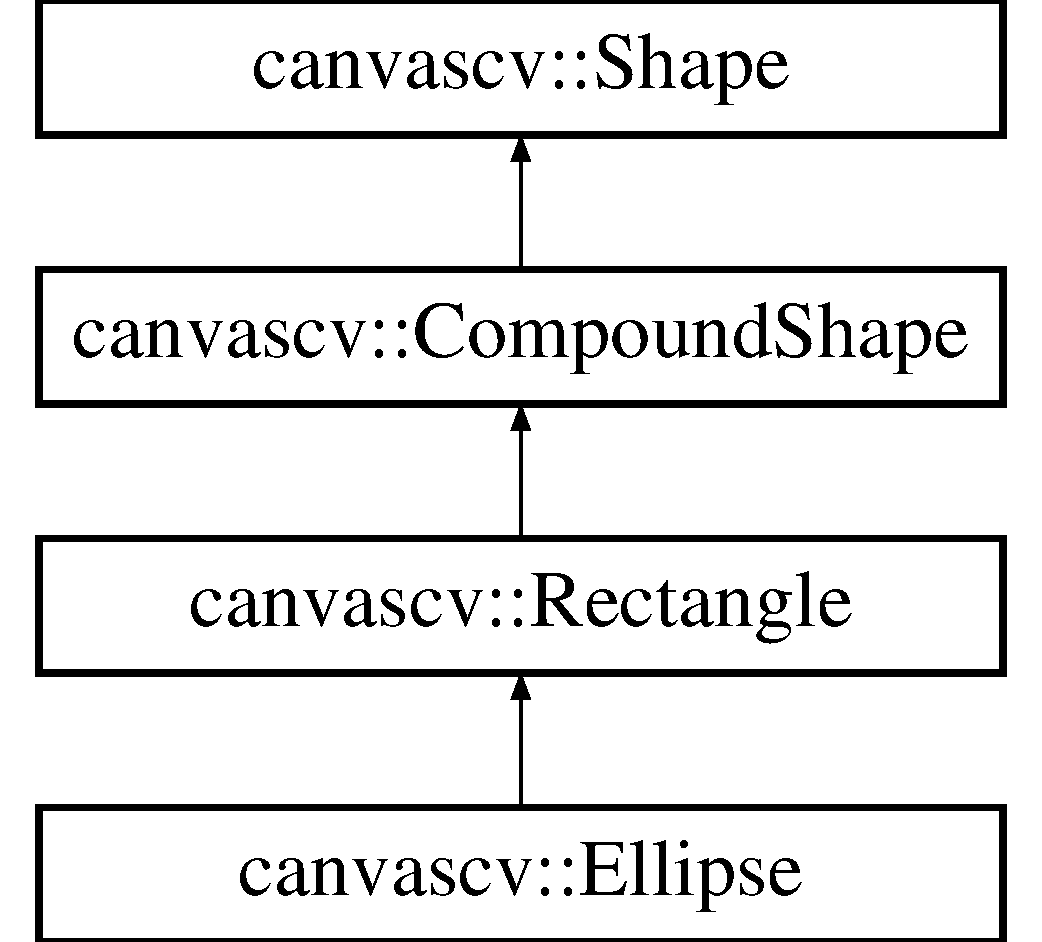
\includegraphics[height=4.000000cm]{classcanvascv_1_1Rectangle}
\end{center}
\end{figure}
\subsection*{Public Member Functions}
\begin{DoxyCompactItemize}
\item 
cv\+::\+Rotated\+Rect \hyperlink{classcanvascv_1_1Rectangle_aa821fa0533fed58ce488d796a25f7d74}{get\+Rect} () const \hypertarget{classcanvascv_1_1Rectangle_aa821fa0533fed58ce488d796a25f7d74}{}\label{classcanvascv_1_1Rectangle_aa821fa0533fed58ce488d796a25f7d74}

\begin{DoxyCompactList}\small\item\em get the Open\+CV representation of this shape \end{DoxyCompactList}\item 
void \hyperlink{classcanvascv_1_1Rectangle_a5149d50c87c3388619ace3badd868f50}{set\+Rect} (const cv\+::\+Rotated\+Rect \&rect)\hypertarget{classcanvascv_1_1Rectangle_a5149d50c87c3388619ace3badd868f50}{}\label{classcanvascv_1_1Rectangle_a5149d50c87c3388619ace3badd868f50}

\begin{DoxyCompactList}\small\item\em set this shape from the Open\+CV representation \end{DoxyCompactList}\item 
virtual bool \hyperlink{classcanvascv_1_1Rectangle_a905ec50de408cbc2df0158bafff210d1}{key\+Pressed} (int \&key)
\begin{DoxyCompactList}\small\item\em key\+Pressed will be called by \hyperlink{classcanvascv_1_1Canvas}{Canvas} for active shapes \end{DoxyCompactList}\item 
bool \hyperlink{classcanvascv_1_1Rectangle_a2562d2ae0fac60c5604b2b5c5a5a24d0}{is\+Point\+In\+Rectangle} (cv\+::\+Point pos)\hypertarget{classcanvascv_1_1Rectangle_a2562d2ae0fac60c5604b2b5c5a5a24d0}{}\label{classcanvascv_1_1Rectangle_a2562d2ae0fac60c5604b2b5c5a5a24d0}

\begin{DoxyCompactList}\small\item\em returns true if pos is in the rectangle representated by this shape \end{DoxyCompactList}\item 
virtual bool \hyperlink{classcanvascv_1_1Rectangle_a90af43d63545f799eda44a7d107358de}{is\+At\+Pos} (const cv\+::\+Point \&pos)\hypertarget{classcanvascv_1_1Rectangle_a90af43d63545f799eda44a7d107358de}{}\label{classcanvascv_1_1Rectangle_a90af43d63545f799eda44a7d107358de}

\begin{DoxyCompactList}\small\item\em returns true if shape is at pos, false otherwise \end{DoxyCompactList}\item 
virtual std\+::list$<$ \hyperlink{classcanvascv_1_1Handle}{Handle} $\ast$ $>$ \hyperlink{classcanvascv_1_1Rectangle_a90f186627bf00deb4ed1050f68190759}{get\+Connection\+Targets} ()
\begin{DoxyCompactList}\small\item\em get\+Connection\+Targets \end{DoxyCompactList}\item 
virtual const char $\ast$ \hyperlink{classcanvascv_1_1Rectangle_aa66625e0e783029524f669a3113020f5}{get\+Type} () const 
\begin{DoxyCompactList}\small\item\em get\+Type is always implemented by derived to return the same static pointer per shape. \end{DoxyCompactList}\end{DoxyCompactItemize}
\subsection*{Protected Member Functions}
\begin{DoxyCompactItemize}
\item 
virtual void \hyperlink{classcanvascv_1_1Rectangle_a6b75f528a26e50c35ef9adead3489fc8}{draw} (cv\+::\+Mat \&canvas)
\begin{DoxyCompactList}\small\item\em draw shape on the canvas \end{DoxyCompactList}\item 
virtual bool \hyperlink{classcanvascv_1_1Rectangle_ac39753497259e3f6a7fdac667cd08596}{mouse\+Pressed} (const cv\+::\+Point \&pos, bool on\+Create=false)
\begin{DoxyCompactList}\small\item\em mouse\+Pressed \end{DoxyCompactList}\item 
virtual bool \hyperlink{classcanvascv_1_1Rectangle_a0e363f915b93526e034dbfd5550597db}{mouse\+Moved} (const cv\+::\+Point \&pos)
\begin{DoxyCompactList}\small\item\em mouse\+Moved \end{DoxyCompactList}\item 
virtual bool \hyperlink{classcanvascv_1_1Rectangle_a6a54774d57d88d053cfb8d5a41878b16}{mouse\+Released} (const cv\+::\+Point \&pos)
\begin{DoxyCompactList}\small\item\em mouse\+Released \end{DoxyCompactList}\end{DoxyCompactItemize}
\subsection*{Additional Inherited Members}


\subsection{Detailed Description}
Allows you to draw a rotatable rectangle by mouse or from code 

\subsection{Member Function Documentation}
\index{canvascv\+::\+Rectangle@{canvascv\+::\+Rectangle}!draw@{draw}}
\index{draw@{draw}!canvascv\+::\+Rectangle@{canvascv\+::\+Rectangle}}
\subsubsection[{\texorpdfstring{draw(cv\+::\+Mat \&canvas)}{draw(cv::Mat &canvas)}}]{\setlength{\rightskip}{0pt plus 5cm}virtual void canvascv\+::\+Rectangle\+::draw (
\begin{DoxyParamCaption}
\item[{cv\+::\+Mat \&}]{canvas}
\end{DoxyParamCaption}
)\hspace{0.3cm}{\ttfamily [protected]}, {\ttfamily [virtual]}}\hypertarget{classcanvascv_1_1Rectangle_a6b75f528a26e50c35ef9adead3489fc8}{}\label{classcanvascv_1_1Rectangle_a6b75f528a26e50c35ef9adead3489fc8}

\begin{DoxyParams}{Parameters}
{\em canvas} & \\
\hline
\end{DoxyParams}


Reimplemented from \hyperlink{classcanvascv_1_1CompoundShape_a6ec60ee0340ed25274e3ac1349345953}{canvascv\+::\+Compound\+Shape}.

\index{canvascv\+::\+Rectangle@{canvascv\+::\+Rectangle}!get\+Connection\+Targets@{get\+Connection\+Targets}}
\index{get\+Connection\+Targets@{get\+Connection\+Targets}!canvascv\+::\+Rectangle@{canvascv\+::\+Rectangle}}
\subsubsection[{\texorpdfstring{get\+Connection\+Targets()}{getConnectionTargets()}}]{\setlength{\rightskip}{0pt plus 5cm}virtual std\+::list$<${\bf Handle} $\ast$$>$ canvascv\+::\+Rectangle\+::get\+Connection\+Targets (
\begin{DoxyParamCaption}
{}
\end{DoxyParamCaption}
)\hspace{0.3cm}{\ttfamily [virtual]}}\hypertarget{classcanvascv_1_1Rectangle_a90f186627bf00deb4ed1050f68190759}{}\label{classcanvascv_1_1Rectangle_a90f186627bf00deb4ed1050f68190759}
Return a list of Handles this shape allows to connect to from other shapes (mainly for \hyperlink{classcanvascv_1_1ShapesConnector}{Shapes\+Connector}) \begin{DoxyReturn}{Returns}
list of \hyperlink{classcanvascv_1_1Handle}{Handle} pointers we \hyperlink{classcanvascv_1_1ShapesConnector}{Shapes\+Connector} can use to connect 
\end{DoxyReturn}


Implements \hyperlink{classcanvascv_1_1Shape_a827822e17e24118e16fa932ac0e71cd2}{canvascv\+::\+Shape}.

\index{canvascv\+::\+Rectangle@{canvascv\+::\+Rectangle}!get\+Type@{get\+Type}}
\index{get\+Type@{get\+Type}!canvascv\+::\+Rectangle@{canvascv\+::\+Rectangle}}
\subsubsection[{\texorpdfstring{get\+Type() const }{getType() const }}]{\setlength{\rightskip}{0pt plus 5cm}virtual const char$\ast$ canvascv\+::\+Rectangle\+::get\+Type (
\begin{DoxyParamCaption}
{}
\end{DoxyParamCaption}
) const\hspace{0.3cm}{\ttfamily [virtual]}}\hypertarget{classcanvascv_1_1Rectangle_aa66625e0e783029524f669a3113020f5}{}\label{classcanvascv_1_1Rectangle_aa66625e0e783029524f669a3113020f5}
\begin{DoxyReturn}{Returns}
const char $\ast$ pointer to string with shape type name 
\end{DoxyReturn}


Implements \hyperlink{classcanvascv_1_1Shape_adee3cc696c7e82b0d2946e7e667ddd46}{canvascv\+::\+Shape}.



Reimplemented in \hyperlink{classcanvascv_1_1Ellipse_a15df73cf790d34b71749ec0e5d6d0331}{canvascv\+::\+Ellipse}.

\index{canvascv\+::\+Rectangle@{canvascv\+::\+Rectangle}!key\+Pressed@{key\+Pressed}}
\index{key\+Pressed@{key\+Pressed}!canvascv\+::\+Rectangle@{canvascv\+::\+Rectangle}}
\subsubsection[{\texorpdfstring{key\+Pressed(int \&key)}{keyPressed(int &key)}}]{\setlength{\rightskip}{0pt plus 5cm}virtual bool canvascv\+::\+Rectangle\+::key\+Pressed (
\begin{DoxyParamCaption}
\item[{int \&}]{key}
\end{DoxyParamCaption}
)\hspace{0.3cm}{\ttfamily [virtual]}}\hypertarget{classcanvascv_1_1Rectangle_a905ec50de408cbc2df0158bafff210d1}{}\label{classcanvascv_1_1Rectangle_a905ec50de408cbc2df0158bafff210d1}

\begin{DoxyParams}{Parameters}
{\em key} & was pressed. You must set it to -\/1 if you consumed it. \\
\hline
\end{DoxyParams}
\begin{DoxyReturn}{Returns}
true if we want to stay in focus and false otherwise 
\end{DoxyReturn}


Reimplemented from \hyperlink{classcanvascv_1_1CompoundShape_ac739f68737099c6f5c6d2c70196cd07b}{canvascv\+::\+Compound\+Shape}.

\index{canvascv\+::\+Rectangle@{canvascv\+::\+Rectangle}!mouse\+Moved@{mouse\+Moved}}
\index{mouse\+Moved@{mouse\+Moved}!canvascv\+::\+Rectangle@{canvascv\+::\+Rectangle}}
\subsubsection[{\texorpdfstring{mouse\+Moved(const cv\+::\+Point \&pos)}{mouseMoved(const cv::Point &pos)}}]{\setlength{\rightskip}{0pt plus 5cm}virtual bool canvascv\+::\+Rectangle\+::mouse\+Moved (
\begin{DoxyParamCaption}
\item[{const cv\+::\+Point \&}]{pos}
\end{DoxyParamCaption}
)\hspace{0.3cm}{\ttfamily [protected]}, {\ttfamily [virtual]}}\hypertarget{classcanvascv_1_1Rectangle_a0e363f915b93526e034dbfd5550597db}{}\label{classcanvascv_1_1Rectangle_a0e363f915b93526e034dbfd5550597db}

\begin{DoxyEnumerate}
\item Was a mouse moved over this shape?
\item If shape is during edit, then these are the mouse position. 
\begin{DoxyParams}{Parameters}
{\em pos} & \\
\hline
\end{DoxyParams}
\begin{DoxyReturn}{Returns}
true if a mouse moved over this shape, or it is during edit. false otherwise. 
\end{DoxyReturn}

\end{DoxyEnumerate}

Reimplemented from \hyperlink{classcanvascv_1_1CompoundShape_a387d1705b99d2053306ffd8d8e67b63b}{canvascv\+::\+Compound\+Shape}.

\index{canvascv\+::\+Rectangle@{canvascv\+::\+Rectangle}!mouse\+Pressed@{mouse\+Pressed}}
\index{mouse\+Pressed@{mouse\+Pressed}!canvascv\+::\+Rectangle@{canvascv\+::\+Rectangle}}
\subsubsection[{\texorpdfstring{mouse\+Pressed(const cv\+::\+Point \&pos, bool on\+Create=false)}{mousePressed(const cv::Point &pos, bool onCreate=false)}}]{\setlength{\rightskip}{0pt plus 5cm}virtual bool canvascv\+::\+Rectangle\+::mouse\+Pressed (
\begin{DoxyParamCaption}
\item[{const cv\+::\+Point \&}]{pos, }
\item[{bool}]{on\+Create = {\ttfamily false}}
\end{DoxyParamCaption}
)\hspace{0.3cm}{\ttfamily [protected]}, {\ttfamily [virtual]}}\hypertarget{classcanvascv_1_1Rectangle_ac39753497259e3f6a7fdac667cd08596}{}\label{classcanvascv_1_1Rectangle_ac39753497259e3f6a7fdac667cd08596}

\begin{DoxyParams}{Parameters}
{\em pos} & \\
\hline
{\em on\+Create} & is true if this is the mouse press which cerated this shape \\
\hline
\end{DoxyParams}
\begin{DoxyReturn}{Returns}
true for keep in focus, false for leave focus 
\end{DoxyReturn}


Reimplemented from \hyperlink{classcanvascv_1_1CompoundShape_a821d046dceaba47114385d1c87e197ce}{canvascv\+::\+Compound\+Shape}.

\index{canvascv\+::\+Rectangle@{canvascv\+::\+Rectangle}!mouse\+Released@{mouse\+Released}}
\index{mouse\+Released@{mouse\+Released}!canvascv\+::\+Rectangle@{canvascv\+::\+Rectangle}}
\subsubsection[{\texorpdfstring{mouse\+Released(const cv\+::\+Point \&pos)}{mouseReleased(const cv::Point &pos)}}]{\setlength{\rightskip}{0pt plus 5cm}virtual bool canvascv\+::\+Rectangle\+::mouse\+Released (
\begin{DoxyParamCaption}
\item[{const cv\+::\+Point \&}]{pos}
\end{DoxyParamCaption}
)\hspace{0.3cm}{\ttfamily [protected]}, {\ttfamily [virtual]}}\hypertarget{classcanvascv_1_1Rectangle_a6a54774d57d88d053cfb8d5a41878b16}{}\label{classcanvascv_1_1Rectangle_a6a54774d57d88d053cfb8d5a41878b16}

\begin{DoxyParams}{Parameters}
{\em pos} & \\
\hline
\end{DoxyParams}
\begin{DoxyReturn}{Returns}
true for keep in focus, false for leave focus 
\end{DoxyReturn}


Reimplemented from \hyperlink{classcanvascv_1_1CompoundShape_a01cf027fd5f7ec96525949d0c8ae08a1}{canvascv\+::\+Compound\+Shape}.



The documentation for this class was generated from the following file\+:\begin{DoxyCompactItemize}
\item 
Canvas\+C\+V-\/doxygen/src/canvascv/shapes/rectangle.\+h\end{DoxyCompactItemize}

\hypertarget{classcanvascv_1_1SelectionBox}{}\section{canvascv\+:\+:Selection\+Box Class Reference}
\label{classcanvascv_1_1SelectionBox}\index{canvascv\+::\+Selection\+Box@{canvascv\+::\+Selection\+Box}}


The \hyperlink{classcanvascv_1_1SelectionBox}{Selection\+Box} class.  




{\ttfamily \#include $<$selectionbox.\+h$>$}

Inheritance diagram for canvascv\+:\+:Selection\+Box\+:\begin{figure}[H]
\begin{center}
\leavevmode
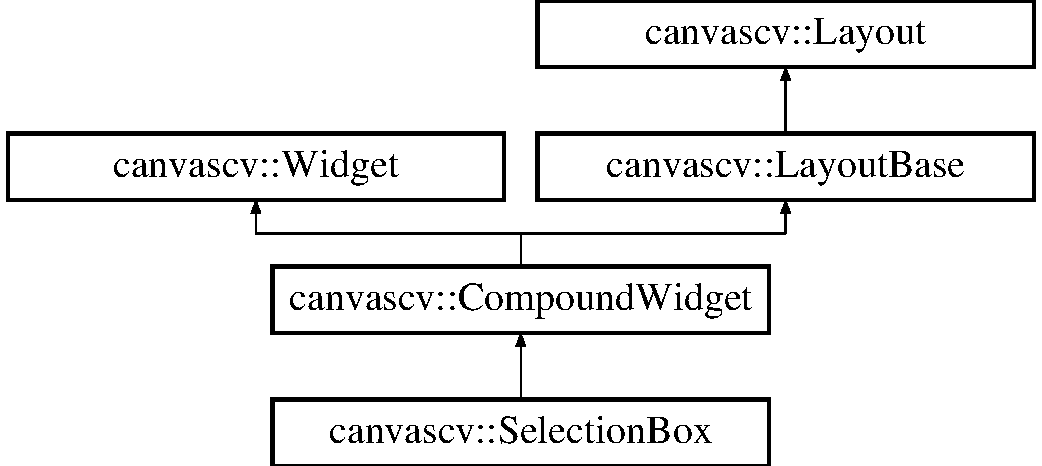
\includegraphics[height=4.000000cm]{classcanvascv_1_1SelectionBox}
\end{center}
\end{figure}
\subsection*{Public Member Functions}
\begin{DoxyCompactItemize}
\item 
std\+::string \hyperlink{classcanvascv_1_1SelectionBox_adb7793b6a0508af80e6320f87549a99e}{get\+Text\+At} (int index) const 
\begin{DoxyCompactList}\small\item\em get\+Text\+At \end{DoxyCompactList}\item 
size\+\_\+t \hyperlink{classcanvascv_1_1SelectionBox_aa24538ddb8d188e7db4c052ba2cf0728}{size} () const \hypertarget{classcanvascv_1_1SelectionBox_aa24538ddb8d188e7db4c052ba2cf0728}{}\label{classcanvascv_1_1SelectionBox_aa24538ddb8d188e7db4c052ba2cf0728}

\begin{DoxyCompactList}\small\item\em return nunmber of check boxes in group \end{DoxyCompactList}\item 
void \hyperlink{classcanvascv_1_1SelectionBox_a760cb57780d64eee6dda96b2971ea3af}{set\+User\+CB} (\hyperlink{classcanvascv_1_1Widget_a977cbd39cf203c5866f07f3645c7e4bc}{Widget\+::\+C\+B\+User\+Selection} cb\+User\+Selection)\hypertarget{classcanvascv_1_1SelectionBox_a760cb57780d64eee6dda96b2971ea3af}{}\label{classcanvascv_1_1SelectionBox_a760cb57780d64eee6dda96b2971ea3af}

\begin{DoxyCompactList}\small\item\em cb\+User\+Selection will be invoked per user selection \end{DoxyCompactList}\item 
virtual const char $\ast$ \hyperlink{classcanvascv_1_1SelectionBox_aef13ee1ea2023ccb5589b6328b458e1c}{get\+Type} () const 
\begin{DoxyCompactList}\small\item\em get\+Type is always implemented by derived to return the same static pointer per widget. \end{DoxyCompactList}\end{DoxyCompactItemize}
\subsection*{Static Public Member Functions}
\begin{DoxyCompactItemize}
\item 
static std\+::shared\+\_\+ptr$<$ \hyperlink{classcanvascv_1_1SelectionBox}{Selection\+Box} $>$ \hyperlink{classcanvascv_1_1SelectionBox_af1f8e0c480d006706bc5240cd1ebd075}{create} (\hyperlink{classcanvascv_1_1Layout}{Layout} \&layout\+Val, std\+::vector$<$ std\+::string $>$ selection\+Names, \hyperlink{classcanvascv_1_1Widget_a977cbd39cf203c5866f07f3645c7e4bc}{Widget\+::\+C\+B\+User\+Selection} cb\+User\+Selection=\hyperlink{classcanvascv_1_1Widget_a977cbd39cf203c5866f07f3645c7e4bc}{Widget\+::\+C\+B\+User\+Selection}(), const cv\+::\+Point \&pos=cv\+::\+Point(0, 0))
\begin{DoxyCompactList}\small\item\em create a selection box widget \end{DoxyCompactList}\end{DoxyCompactItemize}
\subsection*{Protected Member Functions}
\begin{DoxyCompactItemize}
\item 
virtual void \hyperlink{classcanvascv_1_1SelectionBox_a78bf141cda79618e972f173627d07e1a}{recalc\+Compound} ()
\begin{DoxyCompactList}\small\item\em recalc\+Compound \end{DoxyCompactList}\end{DoxyCompactItemize}
\subsection*{Additional Inherited Members}


\subsection{Detailed Description}
Use a message box with any number of buttons on an Open\+CV window \begin{Desc}
\item[Examples\+: ]\par
\hyperlink{example_selectbox_8cpp-example}{example\+\_\+selectbox.\+cpp}.\end{Desc}


\subsection{Member Function Documentation}
\index{canvascv\+::\+Selection\+Box@{canvascv\+::\+Selection\+Box}!create@{create}}
\index{create@{create}!canvascv\+::\+Selection\+Box@{canvascv\+::\+Selection\+Box}}
\subsubsection[{\texorpdfstring{create(\+Layout \&layout\+Val, std\+::vector$<$ std\+::string $>$ selection\+Names, Widget\+::\+C\+B\+User\+Selection cb\+User\+Selection=\+Widget\+::\+C\+B\+User\+Selection(), const cv\+::\+Point \&pos=cv\+::\+Point(0, 0))}{create(Layout &layoutVal, std::vector< std::string > selectionNames, Widget::CBUserSelection cbUserSelection=Widget::CBUserSelection(), const cv::Point &pos=cv::Point(0, 0))}}]{\setlength{\rightskip}{0pt plus 5cm}static std\+::shared\+\_\+ptr$<${\bf Selection\+Box}$>$ canvascv\+::\+Selection\+Box\+::create (
\begin{DoxyParamCaption}
\item[{{\bf Layout} \&}]{layout\+Val, }
\item[{std\+::vector$<$ std\+::string $>$}]{selection\+Names, }
\item[{{\bf Widget\+::\+C\+B\+User\+Selection}}]{cb\+User\+Selection = {\ttfamily {\bf Widget\+::\+C\+B\+User\+Selection}()}, }
\item[{const cv\+::\+Point \&}]{pos = {\ttfamily cv\+:\+:Point(0,~0)}}
\end{DoxyParamCaption}
)\hspace{0.3cm}{\ttfamily [static]}}\hypertarget{classcanvascv_1_1SelectionBox_af1f8e0c480d006706bc5240cd1ebd075}{}\label{classcanvascv_1_1SelectionBox_af1f8e0c480d006706bc5240cd1ebd075}

\begin{DoxyParams}{Parameters}
{\em layout\+Val} & widgets are placed in layouts Canvas/\+V\+Frame/\+H\+Frame/... \\
\hline
{\em selection\+Names} & automatically create items with names of selection\+Names \\
\hline
{\em cb\+User\+Selection} & a callback to invoke with index of pressed button \\
\hline
{\em pos} & location in the \hyperlink{classcanvascv_1_1Layout}{Layout} (if the layout supports Point locations) \\
\hline
\end{DoxyParams}
\begin{DoxyReturn}{Returns}
a smart pointer copy of the object kept in the \hyperlink{classcanvascv_1_1Layout}{Layout} 
\begin{DoxyCode}
Canvas c(winName, image.size());
\textcolor{keyword}{auto} selectionBox = \hyperlink{classcanvascv_1_1SelectionBox_af1f8e0c480d006706bc5240cd1ebd075}{SelectionBox::create}(c, \{
                                        \textcolor{stringliteral}{"Long Option1"},     \textcolor{comment}{// index 0}
                                        \textcolor{stringliteral}{"Option2\(\backslash\)n2 lines"}, \textcolor{comment}{// index 1}
                                        \textcolor{stringliteral}{"Option3"}           \textcolor{comment}{// index 2}
                                    \},
                                    [](Widget *w, \textcolor{keywordtype}{int} i) \{
    w->setVisible(\textcolor{keyword}{false});
    cout << \textcolor{stringliteral}{"Option "} << i << \textcolor{stringliteral}{" was chosen"} << endl;
\});
\textcolor{keywordflow}{while}(...)
\{
    c.\hyperlink{classcanvascv_1_1Canvas_a018c66e277de7904b8146ea3f3feebdd}{redrawOn}(...);
    imshow(...);
    key = c.\hyperlink{classcanvascv_1_1Canvas_a59397db05f5d9e45264f626f6a2ae528}{waitKeyEx}(...); \textcolor{comment}{// GUI and callbacks happen here}
\}
\end{DoxyCode}
 
\end{DoxyReturn}
\begin{Desc}
\item[Examples\+: ]\par
\hyperlink{example_selectbox_8cpp-example}{example\+\_\+selectbox.\+cpp}.\end{Desc}
\index{canvascv\+::\+Selection\+Box@{canvascv\+::\+Selection\+Box}!get\+Text\+At@{get\+Text\+At}}
\index{get\+Text\+At@{get\+Text\+At}!canvascv\+::\+Selection\+Box@{canvascv\+::\+Selection\+Box}}
\subsubsection[{\texorpdfstring{get\+Text\+At(int index) const }{getTextAt(int index) const }}]{\setlength{\rightskip}{0pt plus 5cm}std\+::string canvascv\+::\+Selection\+Box\+::get\+Text\+At (
\begin{DoxyParamCaption}
\item[{int}]{index}
\end{DoxyParamCaption}
) const}\hypertarget{classcanvascv_1_1SelectionBox_adb7793b6a0508af80e6320f87549a99e}{}\label{classcanvascv_1_1SelectionBox_adb7793b6a0508af80e6320f87549a99e}
return the text at index index 
\begin{DoxyParams}{Parameters}
{\em index} & is the index you want the text for \\
\hline
\end{DoxyParams}
\begin{DoxyReturn}{Returns}
return the text at index index or empty string if invalid index 
\end{DoxyReturn}
\begin{Desc}
\item[Examples\+: ]\par
\hyperlink{example_selectbox_8cpp-example}{example\+\_\+selectbox.\+cpp}.\end{Desc}
\index{canvascv\+::\+Selection\+Box@{canvascv\+::\+Selection\+Box}!get\+Type@{get\+Type}}
\index{get\+Type@{get\+Type}!canvascv\+::\+Selection\+Box@{canvascv\+::\+Selection\+Box}}
\subsubsection[{\texorpdfstring{get\+Type() const }{getType() const }}]{\setlength{\rightskip}{0pt plus 5cm}virtual const char$\ast$ canvascv\+::\+Selection\+Box\+::get\+Type (
\begin{DoxyParamCaption}
{}
\end{DoxyParamCaption}
) const\hspace{0.3cm}{\ttfamily [virtual]}}\hypertarget{classcanvascv_1_1SelectionBox_aef13ee1ea2023ccb5589b6328b458e1c}{}\label{classcanvascv_1_1SelectionBox_aef13ee1ea2023ccb5589b6328b458e1c}
\begin{DoxyReturn}{Returns}
const char $\ast$ pointer to string with widget type name 
\end{DoxyReturn}


Implements \hyperlink{classcanvascv_1_1Widget_a85884269bd53ab91203f099a586efa43}{canvascv\+::\+Widget}.

\index{canvascv\+::\+Selection\+Box@{canvascv\+::\+Selection\+Box}!recalc\+Compound@{recalc\+Compound}}
\index{recalc\+Compound@{recalc\+Compound}!canvascv\+::\+Selection\+Box@{canvascv\+::\+Selection\+Box}}
\subsubsection[{\texorpdfstring{recalc\+Compound()}{recalcCompound()}}]{\setlength{\rightskip}{0pt plus 5cm}virtual void canvascv\+::\+Selection\+Box\+::recalc\+Compound (
\begin{DoxyParamCaption}
{}
\end{DoxyParamCaption}
)\hspace{0.3cm}{\ttfamily [protected]}, {\ttfamily [virtual]}}\hypertarget{classcanvascv_1_1SelectionBox_a78bf141cda79618e972f173627d07e1a}{}\label{classcanvascv_1_1SelectionBox_a78bf141cda79618e972f173627d07e1a}
Your BG size recalculation/allocation and FG drawing is done here. It is done semi automatically. Is you invoke setters in this method on your internal widgets, then make sure to update them and/or their layout 

Implements \hyperlink{classcanvascv_1_1CompoundWidget_a4a4f8241d6fd187ffcae2c7968f13864}{canvascv\+::\+Compound\+Widget}.



The documentation for this class was generated from the following file\+:\begin{DoxyCompactItemize}
\item 
Canvas\+C\+V-\/doxygen/src/canvascv/widgets/selectionbox.\+h\end{DoxyCompactItemize}

\hypertarget{classcanvascv_1_1Shape}{}\section{canvascv\+:\+:Shape Class Reference}
\label{classcanvascv_1_1Shape}\index{canvascv\+::\+Shape@{canvascv\+::\+Shape}}


The \hyperlink{classcanvascv_1_1Shape}{Shape} class hierarchy is for geomertric user interaction.  




{\ttfamily \#include $<$shape.\+h$>$}

Inheritance diagram for canvascv\+:\+:Shape\+:\begin{figure}[H]
\begin{center}
\leavevmode
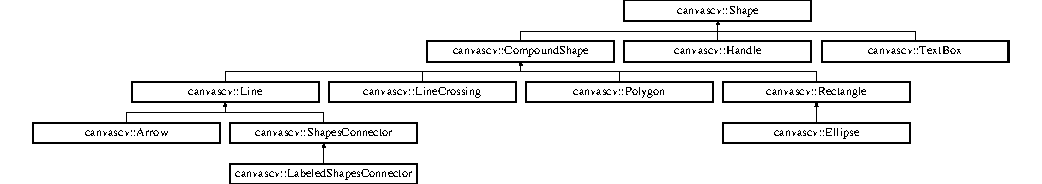
\includegraphics[height=2.466960cm]{classcanvascv_1_1Shape}
\end{center}
\end{figure}
\subsection*{Public Types}
\begin{DoxyCompactItemize}
\item 
typedef std\+::function$<$ void(\hyperlink{classcanvascv_1_1Shape}{Shape} $\ast$, \hyperlink{classcanvascv_1_1Shape_a3fa381d7be3c6bb3cd736e237a444d5c}{Event})$>$ \hyperlink{classcanvascv_1_1Shape_ab36440a99a65779c9b3270dc83625b9b}{C\+B\+Per\+Shape}\hypertarget{classcanvascv_1_1Shape_ab36440a99a65779c9b3270dc83625b9b}{}\label{classcanvascv_1_1Shape_ab36440a99a65779c9b3270dc83625b9b}

\begin{DoxyCompactList}\small\item\em signature of a callback which gets the Event \end{DoxyCompactList}\end{DoxyCompactItemize}
\subsection*{Public Member Functions}
\begin{DoxyCompactItemize}
\item 
\hyperlink{classcanvascv_1_1Shape_a291cd0e85563ad130fdb91882645b3ad}{Shape} ()\hypertarget{classcanvascv_1_1Shape_a291cd0e85563ad130fdb91882645b3ad}{}\label{classcanvascv_1_1Shape_a291cd0e85563ad130fdb91882645b3ad}

\begin{DoxyCompactList}\small\item\em constructor \end{DoxyCompactList}\item 
\hyperlink{classcanvascv_1_1Shape_a625c1941672f157dc6b9fdc83b7f360d}{Shape} (const \hyperlink{classcanvascv_1_1Shape}{Shape} \&other)\hypertarget{classcanvascv_1_1Shape_a625c1941672f157dc6b9fdc83b7f360d}{}\label{classcanvascv_1_1Shape_a625c1941672f157dc6b9fdc83b7f360d}

\begin{DoxyCompactList}\small\item\em copy constructor \end{DoxyCompactList}\item 
virtual \hyperlink{classcanvascv_1_1Shape_a5819d123de258453c06b0e9dcdf60e77}{$\sim$\+Shape} ()\hypertarget{classcanvascv_1_1Shape_a5819d123de258453c06b0e9dcdf60e77}{}\label{classcanvascv_1_1Shape_a5819d123de258453c06b0e9dcdf60e77}

\begin{DoxyCompactList}\small\item\em virtual destructor \end{DoxyCompactList}\item 
void \hyperlink{classcanvascv_1_1Shape_ad2ce0148fa4d79225976334dc1d0d287}{notify\+On\+Event} (\hyperlink{classcanvascv_1_1Shape_ab36440a99a65779c9b3270dc83625b9b}{C\+B\+Per\+Shape} cb)
\begin{DoxyCompactList}\small\item\em used to register for notifications on shape \end{DoxyCompactList}\item 
virtual std\+::list$<$ \hyperlink{classcanvascv_1_1Handle}{Handle} $\ast$ $>$ \hyperlink{classcanvascv_1_1Shape_a827822e17e24118e16fa932ac0e71cd2}{get\+Connection\+Targets} ()=0
\begin{DoxyCompactList}\small\item\em get\+Connection\+Targets \end{DoxyCompactList}\item 
cv\+::\+Scalar \hyperlink{classcanvascv_1_1Shape_a67d3bdec3be2a29c3612c87208589838}{get\+Outline\+Color} () const \hypertarget{classcanvascv_1_1Shape_a67d3bdec3be2a29c3612c87208589838}{}\label{classcanvascv_1_1Shape_a67d3bdec3be2a29c3612c87208589838}

\begin{DoxyCompactList}\small\item\em get the outline color \end{DoxyCompactList}\item 
virtual void \hyperlink{classcanvascv_1_1Shape_adc79bf6f5d81954d743bb255043784f0}{set\+Outline\+Color} (const cv\+::\+Scalar \&value)\hypertarget{classcanvascv_1_1Shape_adc79bf6f5d81954d743bb255043784f0}{}\label{classcanvascv_1_1Shape_adc79bf6f5d81954d743bb255043784f0}

\begin{DoxyCompactList}\small\item\em set the outline color \end{DoxyCompactList}\item 
cv\+::\+Scalar \hyperlink{classcanvascv_1_1Shape_a057f3ea47ffc60678feaa663b375ce27}{get\+Fill\+Color} () const \hypertarget{classcanvascv_1_1Shape_a057f3ea47ffc60678feaa663b375ce27}{}\label{classcanvascv_1_1Shape_a057f3ea47ffc60678feaa663b375ce27}

\begin{DoxyCompactList}\small\item\em get the fill color (fill color is not very useful for shapes right now) \end{DoxyCompactList}\item 
virtual void \hyperlink{classcanvascv_1_1Shape_aee4961631c033ff309e8993c0a8f57b0}{set\+Fill\+Color} (const cv\+::\+Scalar \&value)\hypertarget{classcanvascv_1_1Shape_aee4961631c033ff309e8993c0a8f57b0}{}\label{classcanvascv_1_1Shape_aee4961631c033ff309e8993c0a8f57b0}

\begin{DoxyCompactList}\small\item\em set the fill color (fill color is not very useful for shapes right now) \end{DoxyCompactList}\item 
bool \hyperlink{classcanvascv_1_1Shape_ad343afbb7312ed40e51abefb166cf3dd}{get\+Locked} () const \hypertarget{classcanvascv_1_1Shape_ad343afbb7312ed40e51abefb166cf3dd}{}\label{classcanvascv_1_1Shape_ad343afbb7312ed40e51abefb166cf3dd}

\begin{DoxyCompactList}\small\item\em is the shape locked (can\textquotesingle{}t be moved/edited) \end{DoxyCompactList}\item 
virtual void \hyperlink{classcanvascv_1_1Shape_a3d777d9ff2724ff61c30f45c526354a4}{set\+Locked} (bool value)\hypertarget{classcanvascv_1_1Shape_a3d777d9ff2724ff61c30f45c526354a4}{}\label{classcanvascv_1_1Shape_a3d777d9ff2724ff61c30f45c526354a4}

\begin{DoxyCompactList}\small\item\em set the shape lock state (can/can\textquotesingle{}t be moved/edited) \end{DoxyCompactList}\item 
bool \hyperlink{classcanvascv_1_1Shape_aab29458fc2f7173a2822243f5c5f102e}{get\+Visible} () const \hypertarget{classcanvascv_1_1Shape_aab29458fc2f7173a2822243f5c5f102e}{}\label{classcanvascv_1_1Shape_aab29458fc2f7173a2822243f5c5f102e}

\begin{DoxyCompactList}\small\item\em is the shape visible \end{DoxyCompactList}\item 
virtual void \hyperlink{classcanvascv_1_1Shape_ae35177d229d3e67a39043f82a73fda6a}{set\+Visible} (bool value)\hypertarget{classcanvascv_1_1Shape_ae35177d229d3e67a39043f82a73fda6a}{}\label{classcanvascv_1_1Shape_ae35177d229d3e67a39043f82a73fda6a}

\begin{DoxyCompactList}\small\item\em set the shape visible state \end{DoxyCompactList}\item 
virtual const char $\ast$ \hyperlink{classcanvascv_1_1Shape_adee3cc696c7e82b0d2946e7e667ddd46}{get\+Type} () const =0
\begin{DoxyCompactList}\small\item\em get\+Type is always implemented by derived to return the same static pointer per shape. \end{DoxyCompactList}\item 
int \hyperlink{classcanvascv_1_1Shape_a58991b0f8c38c5ca9a0dabac9a95b8c0}{get\+Thickness} () const \hypertarget{classcanvascv_1_1Shape_a58991b0f8c38c5ca9a0dabac9a95b8c0}{}\label{classcanvascv_1_1Shape_a58991b0f8c38c5ca9a0dabac9a95b8c0}

\begin{DoxyCompactList}\small\item\em get line thickness to use when drawing \end{DoxyCompactList}\item 
virtual void \hyperlink{classcanvascv_1_1Shape_a67c1ccb98b4d24735e368ebbd03fb76d}{set\+Thickness} (int value)\hypertarget{classcanvascv_1_1Shape_a67c1ccb98b4d24735e368ebbd03fb76d}{}\label{classcanvascv_1_1Shape_a67c1ccb98b4d24735e368ebbd03fb76d}

\begin{DoxyCompactList}\small\item\em set line thickness to use when drawing \end{DoxyCompactList}\item 
int \hyperlink{classcanvascv_1_1Shape_a7345362b773e581d7e595e5662491231}{get\+Line\+Type} () const \hypertarget{classcanvascv_1_1Shape_a7345362b773e581d7e595e5662491231}{}\label{classcanvascv_1_1Shape_a7345362b773e581d7e595e5662491231}

\begin{DoxyCompactList}\small\item\em get the line type (L\+I\+N\+E\+\_\+4, L\+I\+N\+E\+\_\+8, L\+I\+N\+E\+\_\+\+AA) \end{DoxyCompactList}\item 
virtual void \hyperlink{classcanvascv_1_1Shape_a83195df4dc837a950462a314467b8114}{set\+Line\+Type} (int value)\hypertarget{classcanvascv_1_1Shape_a83195df4dc837a950462a314467b8114}{}\label{classcanvascv_1_1Shape_a83195df4dc837a950462a314467b8114}

\begin{DoxyCompactList}\small\item\em set the line type (L\+I\+N\+E\+\_\+4, L\+I\+N\+E\+\_\+8, L\+I\+N\+E\+\_\+\+AA) \end{DoxyCompactList}\item 
virtual bool \hyperlink{classcanvascv_1_1Shape_a801866696093d085433d6bf9f256d6f1}{is\+At\+Pos} (const cv\+::\+Point \&pos)=0\hypertarget{classcanvascv_1_1Shape_a801866696093d085433d6bf9f256d6f1}{}\label{classcanvascv_1_1Shape_a801866696093d085433d6bf9f256d6f1}

\begin{DoxyCompactList}\small\item\em returns true if shape is at pos, false otherwise \end{DoxyCompactList}\item 
int \hyperlink{classcanvascv_1_1Shape_a47d76edb7fe4316ce5f8e17a5c38c886}{get\+Id} ()\hypertarget{classcanvascv_1_1Shape_a47d76edb7fe4316ce5f8e17a5c38c886}{}\label{classcanvascv_1_1Shape_a47d76edb7fe4316ce5f8e17a5c38c886}

\begin{DoxyCompactList}\small\item\em return a unique id for this shape \end{DoxyCompactList}\end{DoxyCompactItemize}
\subsection*{Protected Member Functions}
\begin{DoxyCompactItemize}
\item 
virtual bool \hyperlink{classcanvascv_1_1Shape_aa332adef968829dd7744cb1f6a491879}{mouse\+Pressed} (const cv\+::\+Point \&pos, bool on\+Create=false)=0
\begin{DoxyCompactList}\small\item\em mouse\+Pressed \end{DoxyCompactList}\item 
virtual bool \hyperlink{classcanvascv_1_1Shape_acc72c3f645927c135dbc589e2c8678d4}{mouse\+Moved} (const cv\+::\+Point \&pos)=0
\begin{DoxyCompactList}\small\item\em mouse\+Moved \end{DoxyCompactList}\item 
virtual std\+::shared\+\_\+ptr$<$ \hyperlink{classcanvascv_1_1Shape}{Shape} $>$ \hyperlink{classcanvascv_1_1Shape_a89e585b5a1099f5ce291ded14db7181d}{get\+Shape} (int id)
\begin{DoxyCompactList}\small\item\em get\+Shape \end{DoxyCompactList}\item 
virtual bool \hyperlink{classcanvascv_1_1Shape_a7419dc43b9be99010e2b3bb973efbd37}{key\+Pressed} (int \&key)
\begin{DoxyCompactList}\small\item\em key\+Pressed will be called by \hyperlink{classcanvascv_1_1Canvas}{Canvas} for active shapes \end{DoxyCompactList}\item 
virtual void \hyperlink{classcanvascv_1_1Shape_a9682a16069302dfc183ba04f7ad512db}{lost\+Focus} ()\hypertarget{classcanvascv_1_1Shape_a9682a16069302dfc183ba04f7ad512db}{}\label{classcanvascv_1_1Shape_a9682a16069302dfc183ba04f7ad512db}

\begin{DoxyCompactList}\small\item\em lost\+Focus is called by \hyperlink{classcanvascv_1_1Canvas}{Canvas} if we\textquotesingle{}re in it and just became non-\/active \end{DoxyCompactList}\item 
virtual bool \hyperlink{classcanvascv_1_1Shape_a8cbe386ff880c9830c0e4a97b335abf0}{mouse\+Released} (const cv\+::\+Point \&pos)=0
\begin{DoxyCompactList}\small\item\em mouse\+Released \end{DoxyCompactList}\item 
virtual void \hyperlink{classcanvascv_1_1Shape_ab064fdb03d0d94ce84bde0b76b9e62c0}{draw} (cv\+::\+Mat \&canvas)=0
\begin{DoxyCompactList}\small\item\em draw shape on the canvas \end{DoxyCompactList}\item 
void \hyperlink{classcanvascv_1_1Shape_a020a0b73278de5db5404b662b6a41363}{draw\+Helper} (cv\+::\+Mat \&canvas, \hyperlink{classcanvascv_1_1Shape}{Shape} $\ast$other)\hypertarget{classcanvascv_1_1Shape_a020a0b73278de5db5404b662b6a41363}{}\label{classcanvascv_1_1Shape_a020a0b73278de5db5404b662b6a41363}

\begin{DoxyCompactList}\small\item\em helper method for non compund shapes to draw their members \end{DoxyCompactList}\end{DoxyCompactItemize}


\subsection{Detailed Description}
Use shapes to get on screen selections and landmark settings from your user. \begin{DoxySeeAlso}{See also}
\hyperlink{classcanvascv_1_1ThemeRepository}{Theme\+Repository} for using themes. 

\hyperlink{classcanvascv_1_1Canvas}{Canvas} for creating shapes. 
\end{DoxySeeAlso}
\begin{DoxyNote}{Note}
All shapes are create either with the mouse or by the \hyperlink{classcanvascv_1_1Canvas_a630ac92458f1718d0c597e96dd5a4aef}{Canvas\+::create\+Shape()} methods. This method will return a shared\+\_\+ptr$<$\+T$>$ instance, which you don\textquotesingle{}t have to keep since another one is kept by the \hyperlink{classcanvascv_1_1Canvas}{Canvas} in which the shape is placed. Never use delete on a \hyperlink{classcanvascv_1_1Shape}{Shape} pointer. 
\end{DoxyNote}
\begin{Desc}
\item[Examples\+: ]\par
\hyperlink{example_linecrossing_8cpp-example}{example\+\_\+linecrossing.\+cpp}, and \hyperlink{example_shapes_widgets_8cpp-example}{example\+\_\+shapes\+\_\+widgets.\+cpp}.\end{Desc}


\subsection{Member Enumeration Documentation}
\index{canvascv\+::\+Shape@{canvascv\+::\+Shape}!Event@{Event}}
\index{Event@{Event}!canvascv\+::\+Shape@{canvascv\+::\+Shape}}
\subsubsection[{\texorpdfstring{Event}{Event}}]{\setlength{\rightskip}{0pt plus 5cm}enum {\bf canvascv\+::\+Shape\+::\+Event}}\hypertarget{classcanvascv_1_1Shape_a3fa381d7be3c6bb3cd736e237a444d5c}{}\label{classcanvascv_1_1Shape_a3fa381d7be3c6bb3cd736e237a444d5c}
\begin{Desc}
\item[Enumerator]\par
\begin{description}
\index{S\+E\+L\+E\+CT@{S\+E\+L\+E\+CT}!canvascv\+::\+Shape@{canvascv\+::\+Shape}}\index{canvascv\+::\+Shape@{canvascv\+::\+Shape}!S\+E\+L\+E\+CT@{S\+E\+L\+E\+CT}}\item[{\em 
S\+E\+L\+E\+CT\hypertarget{classcanvascv_1_1Shape_a3fa381d7be3c6bb3cd736e237a444d5cafeb2f2cbc576f5235afac464e54a7450}{}\label{classcanvascv_1_1Shape_a3fa381d7be3c6bb3cd736e237a444d5cafeb2f2cbc576f5235afac464e54a7450}
}]shape selected \index{U\+N\+S\+E\+L\+E\+CT@{U\+N\+S\+E\+L\+E\+CT}!canvascv\+::\+Shape@{canvascv\+::\+Shape}}\index{canvascv\+::\+Shape@{canvascv\+::\+Shape}!U\+N\+S\+E\+L\+E\+CT@{U\+N\+S\+E\+L\+E\+CT}}\item[{\em 
U\+N\+S\+E\+L\+E\+CT\hypertarget{classcanvascv_1_1Shape_a3fa381d7be3c6bb3cd736e237a444d5cafea26e438446b822586b19d85b9c1f44}{}\label{classcanvascv_1_1Shape_a3fa381d7be3c6bb3cd736e237a444d5cafea26e438446b822586b19d85b9c1f44}
}]shape unselected \index{R\+E\+M\+O\+V\+ED@{R\+E\+M\+O\+V\+ED}!canvascv\+::\+Shape@{canvascv\+::\+Shape}}\index{canvascv\+::\+Shape@{canvascv\+::\+Shape}!R\+E\+M\+O\+V\+ED@{R\+E\+M\+O\+V\+ED}}\item[{\em 
R\+E\+M\+O\+V\+ED\hypertarget{classcanvascv_1_1Shape_a3fa381d7be3c6bb3cd736e237a444d5caa6787a2dc8627b989f9befaf2e50c9ad}{}\label{classcanvascv_1_1Shape_a3fa381d7be3c6bb3cd736e237a444d5caa6787a2dc8627b989f9befaf2e50c9ad}
}]shape removed \end{description}
\end{Desc}


\subsection{Member Function Documentation}
\index{canvascv\+::\+Shape@{canvascv\+::\+Shape}!draw@{draw}}
\index{draw@{draw}!canvascv\+::\+Shape@{canvascv\+::\+Shape}}
\subsubsection[{\texorpdfstring{draw(cv\+::\+Mat \&canvas)=0}{draw(cv::Mat &canvas)=0}}]{\setlength{\rightskip}{0pt plus 5cm}virtual void canvascv\+::\+Shape\+::draw (
\begin{DoxyParamCaption}
\item[{cv\+::\+Mat \&}]{canvas}
\end{DoxyParamCaption}
)\hspace{0.3cm}{\ttfamily [protected]}, {\ttfamily [pure virtual]}}\hypertarget{classcanvascv_1_1Shape_ab064fdb03d0d94ce84bde0b76b9e62c0}{}\label{classcanvascv_1_1Shape_ab064fdb03d0d94ce84bde0b76b9e62c0}

\begin{DoxyParams}{Parameters}
{\em canvas} & \\
\hline
\end{DoxyParams}


Implemented in \hyperlink{classcanvascv_1_1Line_aad801107019337b6e369fed331539d56}{canvascv\+::\+Line}, \hyperlink{classcanvascv_1_1LineCrossing_a04d251f0cda9f4f51d98d483264fb2dd}{canvascv\+::\+Line\+Crossing}, \hyperlink{classcanvascv_1_1TextBox_a81bf5e2f8c85a805dfff4a401addd0bf}{canvascv\+::\+Text\+Box}, \hyperlink{classcanvascv_1_1Handle_aa1222a3978874c0a9534c2a86ef8b51f}{canvascv\+::\+Handle}, \hyperlink{classcanvascv_1_1Polygon_a32e073cb9579fdf4645daf14e5143f22}{canvascv\+::\+Polygon}, \hyperlink{classcanvascv_1_1Rectangle_a6b75f528a26e50c35ef9adead3489fc8}{canvascv\+::\+Rectangle}, \hyperlink{classcanvascv_1_1CompoundShape_a6ec60ee0340ed25274e3ac1349345953}{canvascv\+::\+Compound\+Shape}, and \hyperlink{classcanvascv_1_1Arrow_a8ba5b890df49a2d8fc6630df5fe80351}{canvascv\+::\+Arrow}.

\index{canvascv\+::\+Shape@{canvascv\+::\+Shape}!get\+Connection\+Targets@{get\+Connection\+Targets}}
\index{get\+Connection\+Targets@{get\+Connection\+Targets}!canvascv\+::\+Shape@{canvascv\+::\+Shape}}
\subsubsection[{\texorpdfstring{get\+Connection\+Targets()=0}{getConnectionTargets()=0}}]{\setlength{\rightskip}{0pt plus 5cm}virtual std\+::list$<${\bf Handle}$\ast$$>$ canvascv\+::\+Shape\+::get\+Connection\+Targets (
\begin{DoxyParamCaption}
{}
\end{DoxyParamCaption}
)\hspace{0.3cm}{\ttfamily [pure virtual]}}\hypertarget{classcanvascv_1_1Shape_a827822e17e24118e16fa932ac0e71cd2}{}\label{classcanvascv_1_1Shape_a827822e17e24118e16fa932ac0e71cd2}
Return a list of Handles this shape allows to connect to from other shapes (mainly for \hyperlink{classcanvascv_1_1ShapesConnector}{Shapes\+Connector}) \begin{DoxyReturn}{Returns}
list of \hyperlink{classcanvascv_1_1Handle}{Handle} pointers we \hyperlink{classcanvascv_1_1ShapesConnector}{Shapes\+Connector} can use to connect 
\end{DoxyReturn}


Implemented in \hyperlink{classcanvascv_1_1Line_a4a4293ae8f9600ee7f9d3a8089e6965a}{canvascv\+::\+Line}, \hyperlink{classcanvascv_1_1LineCrossing_a8428e287e407e07cfaf11ea6d655e0e6}{canvascv\+::\+Line\+Crossing}, \hyperlink{classcanvascv_1_1ShapesConnector_a90672acd22f69f3d143f08197d4108b8}{canvascv\+::\+Shapes\+Connector}, \hyperlink{classcanvascv_1_1Handle_a6cf6d2c4ad6a01a1e9e7c27f3c29ed57}{canvascv\+::\+Handle}, \hyperlink{classcanvascv_1_1TextBox_aef1fa0cd32292635c1b92b6ecd8b4aad}{canvascv\+::\+Text\+Box}, \hyperlink{classcanvascv_1_1Polygon_a4e15fc33d4dceb99e4f063b5dda2e658}{canvascv\+::\+Polygon}, and \hyperlink{classcanvascv_1_1Rectangle_a90f186627bf00deb4ed1050f68190759}{canvascv\+::\+Rectangle}.

\index{canvascv\+::\+Shape@{canvascv\+::\+Shape}!get\+Shape@{get\+Shape}}
\index{get\+Shape@{get\+Shape}!canvascv\+::\+Shape@{canvascv\+::\+Shape}}
\subsubsection[{\texorpdfstring{get\+Shape(int id)}{getShape(int id)}}]{\setlength{\rightskip}{0pt plus 5cm}virtual std\+::shared\+\_\+ptr$<${\bf Shape}$>$ canvascv\+::\+Shape\+::get\+Shape (
\begin{DoxyParamCaption}
\item[{int}]{id}
\end{DoxyParamCaption}
)\hspace{0.3cm}{\ttfamily [protected]}, {\ttfamily [virtual]}}\hypertarget{classcanvascv_1_1Shape_a89e585b5a1099f5ce291ded14db7181d}{}\label{classcanvascv_1_1Shape_a89e585b5a1099f5ce291ded14db7181d}
Get internal shapes, which \hyperlink{classcanvascv_1_1Canvas}{Canvas} doesn\textquotesingle{}t know of. 
\begin{DoxyParams}{Parameters}
{\em id} & \\
\hline
\end{DoxyParams}
\begin{DoxyReturn}{Returns}
internal sub shape with requested id 
\end{DoxyReturn}


Reimplemented in \hyperlink{classcanvascv_1_1TextBox_a100b59e6be1b9f9290e03654061c0ec1}{canvascv\+::\+Text\+Box}, and \hyperlink{classcanvascv_1_1CompoundShape_aa9ef6ed91e5a2b6fbd3efe13fbd8e561}{canvascv\+::\+Compound\+Shape}.

\index{canvascv\+::\+Shape@{canvascv\+::\+Shape}!get\+Type@{get\+Type}}
\index{get\+Type@{get\+Type}!canvascv\+::\+Shape@{canvascv\+::\+Shape}}
\subsubsection[{\texorpdfstring{get\+Type() const =0}{getType() const =0}}]{\setlength{\rightskip}{0pt plus 5cm}virtual const char$\ast$ canvascv\+::\+Shape\+::get\+Type (
\begin{DoxyParamCaption}
{}
\end{DoxyParamCaption}
) const\hspace{0.3cm}{\ttfamily [pure virtual]}}\hypertarget{classcanvascv_1_1Shape_adee3cc696c7e82b0d2946e7e667ddd46}{}\label{classcanvascv_1_1Shape_adee3cc696c7e82b0d2946e7e667ddd46}
\begin{DoxyReturn}{Returns}
const char $\ast$ pointer to string with shape type name 
\end{DoxyReturn}


Implemented in \hyperlink{classcanvascv_1_1Line_a863306159fbca892702fd3d0047b63c3}{canvascv\+::\+Line}, \hyperlink{classcanvascv_1_1LineCrossing_a86757b4f629d3d03885f62976d5b7fc3}{canvascv\+::\+Line\+Crossing}, \hyperlink{classcanvascv_1_1TextBox_aa9313765c2040647a8fc32d227139c4d}{canvascv\+::\+Text\+Box}, \hyperlink{classcanvascv_1_1ShapesConnector_aedda9e8fd9c1be85704f289df94905a2}{canvascv\+::\+Shapes\+Connector}, \hyperlink{classcanvascv_1_1Handle_a6d255d8bfe17209610ffb0143903dbdc}{canvascv\+::\+Handle}, \hyperlink{classcanvascv_1_1Polygon_a58dab27bcdfcaab026e0e79157e68318}{canvascv\+::\+Polygon}, \hyperlink{classcanvascv_1_1Rectangle_aa66625e0e783029524f669a3113020f5}{canvascv\+::\+Rectangle}, \hyperlink{classcanvascv_1_1LabeledShapesConnector_aebeccdf1e7c4efb0bde504b361eac801}{canvascv\+::\+Labeled\+Shapes\+Connector}, \hyperlink{classcanvascv_1_1Arrow_a4d0857dec7276f993bd390e944edef34}{canvascv\+::\+Arrow}, and \hyperlink{classcanvascv_1_1Ellipse_a15df73cf790d34b71749ec0e5d6d0331}{canvascv\+::\+Ellipse}.

\begin{Desc}
\item[Examples\+: ]\par
\hyperlink{example_linecrossing_8cpp-example}{example\+\_\+linecrossing.\+cpp}, and \hyperlink{example_shapes_widgets_8cpp-example}{example\+\_\+shapes\+\_\+widgets.\+cpp}.\end{Desc}
\index{canvascv\+::\+Shape@{canvascv\+::\+Shape}!key\+Pressed@{key\+Pressed}}
\index{key\+Pressed@{key\+Pressed}!canvascv\+::\+Shape@{canvascv\+::\+Shape}}
\subsubsection[{\texorpdfstring{key\+Pressed(int \&key)}{keyPressed(int &key)}}]{\setlength{\rightskip}{0pt plus 5cm}virtual bool canvascv\+::\+Shape\+::key\+Pressed (
\begin{DoxyParamCaption}
\item[{int \&}]{key}
\end{DoxyParamCaption}
)\hspace{0.3cm}{\ttfamily [protected]}, {\ttfamily [virtual]}}\hypertarget{classcanvascv_1_1Shape_a7419dc43b9be99010e2b3bb973efbd37}{}\label{classcanvascv_1_1Shape_a7419dc43b9be99010e2b3bb973efbd37}

\begin{DoxyParams}{Parameters}
{\em key} & was pressed. You must set it to -\/1 if you consumed it. \\
\hline
\end{DoxyParams}
\begin{DoxyReturn}{Returns}
true if we want to stay in focus and false otherwise 
\end{DoxyReturn}


Reimplemented in \hyperlink{classcanvascv_1_1Line_a4059736cde05ffc90dda8ed1ff4f9ba2}{canvascv\+::\+Line}, \hyperlink{classcanvascv_1_1TextBox_a4b9a7ecf58369f2161382d3c791542d7}{canvascv\+::\+Text\+Box}, \hyperlink{classcanvascv_1_1Polygon_aca22b914de1ced559faf4fd5426073ff}{canvascv\+::\+Polygon}, \hyperlink{classcanvascv_1_1CompoundShape_ac739f68737099c6f5c6d2c70196cd07b}{canvascv\+::\+Compound\+Shape}, and \hyperlink{classcanvascv_1_1Rectangle_a905ec50de408cbc2df0158bafff210d1}{canvascv\+::\+Rectangle}.

\index{canvascv\+::\+Shape@{canvascv\+::\+Shape}!mouse\+Moved@{mouse\+Moved}}
\index{mouse\+Moved@{mouse\+Moved}!canvascv\+::\+Shape@{canvascv\+::\+Shape}}
\subsubsection[{\texorpdfstring{mouse\+Moved(const cv\+::\+Point \&pos)=0}{mouseMoved(const cv::Point &pos)=0}}]{\setlength{\rightskip}{0pt plus 5cm}virtual bool canvascv\+::\+Shape\+::mouse\+Moved (
\begin{DoxyParamCaption}
\item[{const cv\+::\+Point \&}]{pos}
\end{DoxyParamCaption}
)\hspace{0.3cm}{\ttfamily [protected]}, {\ttfamily [pure virtual]}}\hypertarget{classcanvascv_1_1Shape_acc72c3f645927c135dbc589e2c8678d4}{}\label{classcanvascv_1_1Shape_acc72c3f645927c135dbc589e2c8678d4}

\begin{DoxyEnumerate}
\item Was a mouse moved over this shape?
\item If shape is during edit, then these are the mouse position. 
\begin{DoxyParams}{Parameters}
{\em pos} & \\
\hline
\end{DoxyParams}
\begin{DoxyReturn}{Returns}
true if a mouse moved over this shape, or it is during edit. false otherwise. 
\end{DoxyReturn}

\end{DoxyEnumerate}

Implemented in \hyperlink{classcanvascv_1_1Line_ad758464d98d455d2ea3aa591667fb595}{canvascv\+::\+Line}, \hyperlink{classcanvascv_1_1TextBox_a019cfc3fe096a51c65cc871d4e8be0b7}{canvascv\+::\+Text\+Box}, \hyperlink{classcanvascv_1_1Handle_a68dee628b020ae4360e90c58b51d5291}{canvascv\+::\+Handle}, \hyperlink{classcanvascv_1_1Polygon_aacc442ef4c0438ddb78c6ccce8e86618}{canvascv\+::\+Polygon}, \hyperlink{classcanvascv_1_1Rectangle_a0e363f915b93526e034dbfd5550597db}{canvascv\+::\+Rectangle}, and \hyperlink{classcanvascv_1_1CompoundShape_a387d1705b99d2053306ffd8d8e67b63b}{canvascv\+::\+Compound\+Shape}.

\index{canvascv\+::\+Shape@{canvascv\+::\+Shape}!mouse\+Pressed@{mouse\+Pressed}}
\index{mouse\+Pressed@{mouse\+Pressed}!canvascv\+::\+Shape@{canvascv\+::\+Shape}}
\subsubsection[{\texorpdfstring{mouse\+Pressed(const cv\+::\+Point \&pos, bool on\+Create=false)=0}{mousePressed(const cv::Point &pos, bool onCreate=false)=0}}]{\setlength{\rightskip}{0pt plus 5cm}virtual bool canvascv\+::\+Shape\+::mouse\+Pressed (
\begin{DoxyParamCaption}
\item[{const cv\+::\+Point \&}]{pos, }
\item[{bool}]{on\+Create = {\ttfamily false}}
\end{DoxyParamCaption}
)\hspace{0.3cm}{\ttfamily [protected]}, {\ttfamily [pure virtual]}}\hypertarget{classcanvascv_1_1Shape_aa332adef968829dd7744cb1f6a491879}{}\label{classcanvascv_1_1Shape_aa332adef968829dd7744cb1f6a491879}

\begin{DoxyParams}{Parameters}
{\em pos} & \\
\hline
{\em on\+Create} & is true if this is the mouse press which cerated this shape \\
\hline
\end{DoxyParams}
\begin{DoxyReturn}{Returns}
true for keep in focus, false for leave focus 
\end{DoxyReturn}


Implemented in \hyperlink{classcanvascv_1_1Line_aab4d23d336fe71c6d7000d8da9a54269}{canvascv\+::\+Line}, \hyperlink{classcanvascv_1_1LineCrossing_a8232b4101d5533b12129c4d145ffc54d}{canvascv\+::\+Line\+Crossing}, \hyperlink{classcanvascv_1_1TextBox_adaf9422ce68a31eda4fc683ee0b74b8a}{canvascv\+::\+Text\+Box}, \hyperlink{classcanvascv_1_1Handle_ab6b57f86c6c8ae1385b495b9f790c742}{canvascv\+::\+Handle}, \hyperlink{classcanvascv_1_1ShapesConnector_a6c6400403c6c2809af1e0a64e477f592}{canvascv\+::\+Shapes\+Connector}, \hyperlink{classcanvascv_1_1Polygon_a87ce20dbc22fd0ce39d6e81de5e515ae}{canvascv\+::\+Polygon}, \hyperlink{classcanvascv_1_1Rectangle_ac39753497259e3f6a7fdac667cd08596}{canvascv\+::\+Rectangle}, and \hyperlink{classcanvascv_1_1CompoundShape_a821d046dceaba47114385d1c87e197ce}{canvascv\+::\+Compound\+Shape}.

\index{canvascv\+::\+Shape@{canvascv\+::\+Shape}!mouse\+Released@{mouse\+Released}}
\index{mouse\+Released@{mouse\+Released}!canvascv\+::\+Shape@{canvascv\+::\+Shape}}
\subsubsection[{\texorpdfstring{mouse\+Released(const cv\+::\+Point \&pos)=0}{mouseReleased(const cv::Point &pos)=0}}]{\setlength{\rightskip}{0pt plus 5cm}virtual bool canvascv\+::\+Shape\+::mouse\+Released (
\begin{DoxyParamCaption}
\item[{const cv\+::\+Point \&}]{pos}
\end{DoxyParamCaption}
)\hspace{0.3cm}{\ttfamily [protected]}, {\ttfamily [pure virtual]}}\hypertarget{classcanvascv_1_1Shape_a8cbe386ff880c9830c0e4a97b335abf0}{}\label{classcanvascv_1_1Shape_a8cbe386ff880c9830c0e4a97b335abf0}

\begin{DoxyParams}{Parameters}
{\em pos} & \\
\hline
\end{DoxyParams}
\begin{DoxyReturn}{Returns}
true for keep in focus, false for leave focus 
\end{DoxyReturn}


Implemented in \hyperlink{classcanvascv_1_1Line_ace7269cabd2acbb2c9da009740f46fa3}{canvascv\+::\+Line}, \hyperlink{classcanvascv_1_1TextBox_ad048ee21fc55f500c6c85755d2d87aeb}{canvascv\+::\+Text\+Box}, \hyperlink{classcanvascv_1_1Handle_a9d6a7db28837396d45b90db7bce79b76}{canvascv\+::\+Handle}, \hyperlink{classcanvascv_1_1ShapesConnector_a56ab827f3d72e495ccfd1101807413f8}{canvascv\+::\+Shapes\+Connector}, \hyperlink{classcanvascv_1_1Polygon_afea6bbe1beef916e6ec47ed257cb2374}{canvascv\+::\+Polygon}, \hyperlink{classcanvascv_1_1Rectangle_a6a54774d57d88d053cfb8d5a41878b16}{canvascv\+::\+Rectangle}, and \hyperlink{classcanvascv_1_1CompoundShape_a01cf027fd5f7ec96525949d0c8ae08a1}{canvascv\+::\+Compound\+Shape}.

\index{canvascv\+::\+Shape@{canvascv\+::\+Shape}!notify\+On\+Event@{notify\+On\+Event}}
\index{notify\+On\+Event@{notify\+On\+Event}!canvascv\+::\+Shape@{canvascv\+::\+Shape}}
\subsubsection[{\texorpdfstring{notify\+On\+Event(\+C\+B\+Per\+Shape cb)}{notifyOnEvent(CBPerShape cb)}}]{\setlength{\rightskip}{0pt plus 5cm}void canvascv\+::\+Shape\+::notify\+On\+Event (
\begin{DoxyParamCaption}
\item[{{\bf C\+B\+Per\+Shape}}]{cb}
\end{DoxyParamCaption}
)}\hypertarget{classcanvascv_1_1Shape_ad2ce0148fa4d79225976334dc1d0d287}{}\label{classcanvascv_1_1Shape_ad2ce0148fa4d79225976334dc1d0d287}

\begin{DoxyParams}{Parameters}
{\em cb} & to invoke on shape event \\
\hline
\end{DoxyParams}


The documentation for this class was generated from the following file\+:\begin{DoxyCompactItemize}
\item 
Canvas\+C\+V-\/doxygen/src/canvascv/shapes/shape.\+h\end{DoxyCompactItemize}

\hypertarget{classcanvascv_1_1ShapeFactory}{}\section{canvascv\+:\+:Shape\+Factory Class Reference}
\label{classcanvascv_1_1ShapeFactory}\index{canvascv\+::\+Shape\+Factory@{canvascv\+::\+Shape\+Factory}}


The \hyperlink{classcanvascv_1_1ShapeFactory}{Shape\+Factory} class.  




{\ttfamily \#include $<$shapefactory.\+h$>$}

Inheritance diagram for canvascv\+:\+:Shape\+Factory\+:\begin{figure}[H]
\begin{center}
\leavevmode
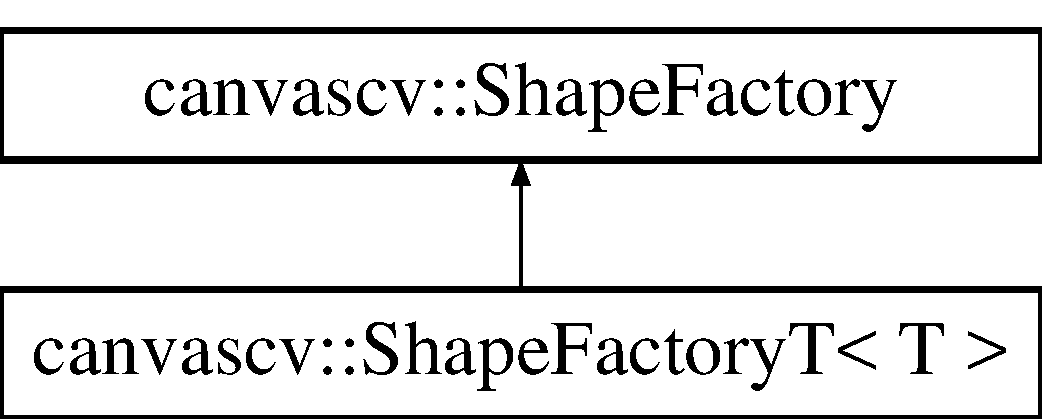
\includegraphics[height=2.000000cm]{classcanvascv_1_1ShapeFactory}
\end{center}
\end{figure}
\subsection*{Static Public Member Functions}
\begin{DoxyCompactItemize}
\item 
static \hyperlink{classcanvascv_1_1Shape}{Shape} $\ast$ \hyperlink{classcanvascv_1_1ShapeFactory_ac21c83f31513026566111cad2a63d359}{new\+Shape} (std\+::string type, const cv\+::\+Point \&pos)\hypertarget{classcanvascv_1_1ShapeFactory_ac21c83f31513026566111cad2a63d359}{}\label{classcanvascv_1_1ShapeFactory_ac21c83f31513026566111cad2a63d359}

\begin{DoxyCompactList}\small\item\em create a shape by type name at a certain initial pos (don\textquotesingle{}t use directly. Use \hyperlink{classcanvascv_1_1Canvas_a630ac92458f1718d0c597e96dd5a4aef}{Canvas\+::create\+Shape()} instead). \end{DoxyCompactList}\end{DoxyCompactItemize}


\subsection{Detailed Description}
Holds shape creation methods. Don\textquotesingle{}t use directly. Use \hyperlink{classcanvascv_1_1Canvas_a630ac92458f1718d0c597e96dd5a4aef}{Canvas\+::create\+Shape()} instead. \begin{DoxySeeAlso}{See also}
\hyperlink{classcanvascv_1_1Canvas_a630ac92458f1718d0c597e96dd5a4aef}{Canvas\+::create\+Shape()} 
\end{DoxySeeAlso}


The documentation for this class was generated from the following file\+:\begin{DoxyCompactItemize}
\item 
Canvas\+C\+V-\/doxygen/src/canvascv/shapes/shapefactory.\+h\end{DoxyCompactItemize}

\hypertarget{classcanvascv_1_1ShapeFactoryT}{}\section{canvascv\+:\+:Shape\+FactoryT$<$ T $>$ Class Template Reference}
\label{classcanvascv_1_1ShapeFactoryT}\index{canvascv\+::\+Shape\+Factory\+T$<$ T $>$@{canvascv\+::\+Shape\+Factory\+T$<$ T $>$}}


The \hyperlink{classcanvascv_1_1ShapeFactoryT}{Shape\+FactoryT} class.  




{\ttfamily \#include $<$shapefactory.\+h$>$}

Inheritance diagram for canvascv\+:\+:Shape\+FactoryT$<$ T $>$\+:\begin{figure}[H]
\begin{center}
\leavevmode
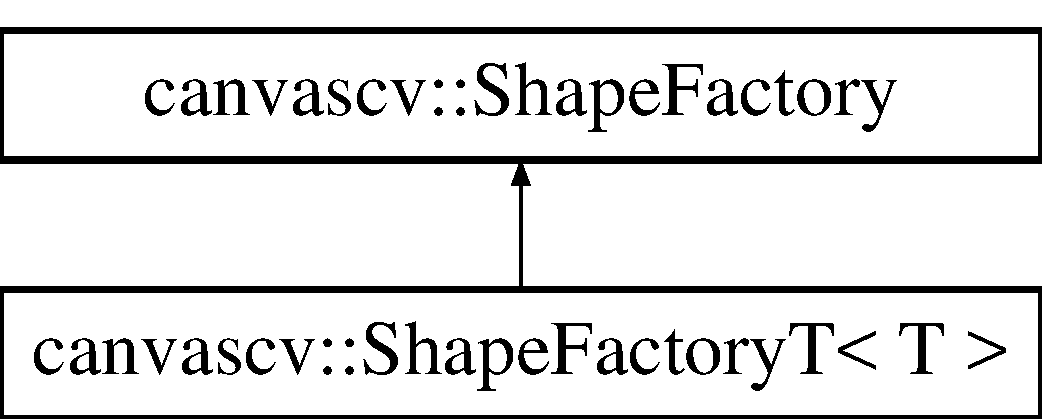
\includegraphics[height=2.000000cm]{classcanvascv_1_1ShapeFactoryT}
\end{center}
\end{figure}
\subsection*{Static Public Member Functions}
\begin{DoxyCompactItemize}
\item 
static bool \hyperlink{classcanvascv_1_1ShapeFactoryT_a7d2e3d1e856ba83cb107439ceee53229}{add\+Type} (std\+::string name)\hypertarget{classcanvascv_1_1ShapeFactoryT_a7d2e3d1e856ba83cb107439ceee53229}{}\label{classcanvascv_1_1ShapeFactoryT_a7d2e3d1e856ba83cb107439ceee53229}

\begin{DoxyCompactList}\small\item\em add a shape by compile time type -\/ use the macro C\+C\+V\+\_\+\+R\+E\+G\+I\+S\+T\+E\+R\+\_\+\+S\+H\+A\+PE \end{DoxyCompactList}\item 
static T $\ast$ \hyperlink{classcanvascv_1_1ShapeFactoryT_a0a0a0d4bae966b362ca68485d34fe1ae}{new\+Shape} (const cv\+::\+Point \&pos)\hypertarget{classcanvascv_1_1ShapeFactoryT_a0a0a0d4bae966b362ca68485d34fe1ae}{}\label{classcanvascv_1_1ShapeFactoryT_a0a0a0d4bae966b362ca68485d34fe1ae}

\begin{DoxyCompactList}\small\item\em create a shape by compile time type at a certain initial pos (don\textquotesingle{}t use directly. Use \hyperlink{classcanvascv_1_1Canvas_a630ac92458f1718d0c597e96dd5a4aef}{Canvas\+::create\+Shape()} instead) \end{DoxyCompactList}\end{DoxyCompactItemize}


\subsection{Detailed Description}
\subsubsection*{template$<$class T$>$\\*
class canvascv\+::\+Shape\+Factory\+T$<$ T $>$}

Holds shape creation methods. Don\textquotesingle{}t use directly. Use \hyperlink{classcanvascv_1_1Canvas_a630ac92458f1718d0c597e96dd5a4aef}{Canvas\+::create\+Shape()} instead. \begin{DoxySeeAlso}{See also}
\hyperlink{classcanvascv_1_1Canvas_a630ac92458f1718d0c597e96dd5a4aef}{Canvas\+::create\+Shape()} 
\end{DoxySeeAlso}


The documentation for this class was generated from the following file\+:\begin{DoxyCompactItemize}
\item 
Canvas\+C\+V-\/doxygen/src/canvascv/shapes/shapefactory.\+h\end{DoxyCompactItemize}

\hypertarget{classcanvascv_1_1ShapesConnector}{}\section{canvascv\+:\+:Shapes\+Connector Class Reference}
\label{classcanvascv_1_1ShapesConnector}\index{canvascv\+::\+Shapes\+Connector@{canvascv\+::\+Shapes\+Connector}}


The \hyperlink{classcanvascv_1_1ShapesConnector}{Shapes\+Connector} class.  




{\ttfamily \#include $<$shapesconnector.\+h$>$}

Inheritance diagram for canvascv\+:\+:Shapes\+Connector\+:\begin{figure}[H]
\begin{center}
\leavevmode
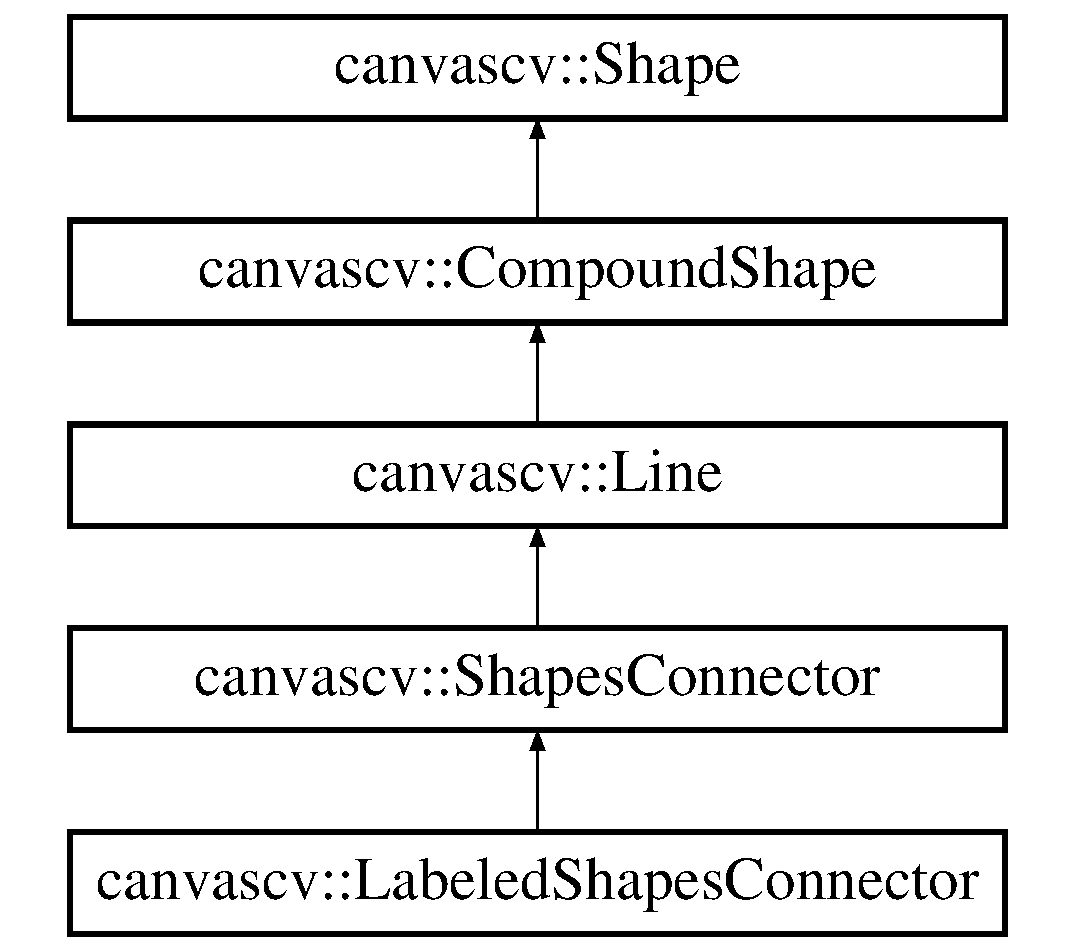
\includegraphics[height=5.000000cm]{classcanvascv_1_1ShapesConnector}
\end{center}
\end{figure}
\subsection*{Public Member Functions}
\begin{DoxyCompactItemize}
\item 
int \hyperlink{classcanvascv_1_1ShapesConnector_ac03d532ffefce9ce5033676a672b0b37}{get\+Spacing} () const \hypertarget{classcanvascv_1_1ShapesConnector_ac03d532ffefce9ce5033676a672b0b37}{}\label{classcanvascv_1_1ShapesConnector_ac03d532ffefce9ce5033676a672b0b37}

\begin{DoxyCompactList}\small\item\em get the spacing of the dotted connecting line \end{DoxyCompactList}\item 
void \hyperlink{classcanvascv_1_1ShapesConnector_aaa6f3f712c905df1c6dd33e535920293}{set\+Spacing} (int value)\hypertarget{classcanvascv_1_1ShapesConnector_aaa6f3f712c905df1c6dd33e535920293}{}\label{classcanvascv_1_1ShapesConnector_aaa6f3f712c905df1c6dd33e535920293}

\begin{DoxyCompactList}\small\item\em set the spacing of the dotted connecting line \end{DoxyCompactList}\item 
void \hyperlink{classcanvascv_1_1ShapesConnector_a949cf82640ba6977d8d1879702d1be89}{connect\+Tail} (\hyperlink{classcanvascv_1_1Shape}{Shape} \&shape, \hyperlink{classcanvascv_1_1Handle}{Handle} \&handle)\hypertarget{classcanvascv_1_1ShapesConnector_a949cf82640ba6977d8d1879702d1be89}{}\label{classcanvascv_1_1ShapesConnector_a949cf82640ba6977d8d1879702d1be89}

\begin{DoxyCompactList}\small\item\em Connect \textquotesingle{}shape\textquotesingle{} with it\textquotesingle{}s \hyperlink{classcanvascv_1_1Handle}{Handle} \textquotesingle{}handle\textquotesingle{} to our own tail \hyperlink{classcanvascv_1_1Handle}{Handle}. \end{DoxyCompactList}\item 
void \hyperlink{classcanvascv_1_1ShapesConnector_a1765b937ee22f9b3bf6920b0e1e4767c}{connect\+Head} (\hyperlink{classcanvascv_1_1Shape}{Shape} \&shape, \hyperlink{classcanvascv_1_1Handle}{Handle} \&handle)\hypertarget{classcanvascv_1_1ShapesConnector_a1765b937ee22f9b3bf6920b0e1e4767c}{}\label{classcanvascv_1_1ShapesConnector_a1765b937ee22f9b3bf6920b0e1e4767c}

\begin{DoxyCompactList}\small\item\em Connect \textquotesingle{}shape\textquotesingle{} with it\textquotesingle{}s \hyperlink{classcanvascv_1_1Handle}{Handle} \textquotesingle{}handle\textquotesingle{} to our own head \hyperlink{classcanvascv_1_1Handle}{Handle}. \end{DoxyCompactList}\item 
void \hyperlink{classcanvascv_1_1ShapesConnector_a583c55abfaccaf62f510281b56cc5059}{disconnect\+Tail} ()\hypertarget{classcanvascv_1_1ShapesConnector_a583c55abfaccaf62f510281b56cc5059}{}\label{classcanvascv_1_1ShapesConnector_a583c55abfaccaf62f510281b56cc5059}

\begin{DoxyCompactList}\small\item\em disconnect our own tail \hyperlink{classcanvascv_1_1Handle}{Handle} from any previously connected shape \end{DoxyCompactList}\item 
void \hyperlink{classcanvascv_1_1ShapesConnector_ae953fce050f2ceffa4eb2c17be416a84}{disconnect\+Head} ()\hypertarget{classcanvascv_1_1ShapesConnector_ae953fce050f2ceffa4eb2c17be416a84}{}\label{classcanvascv_1_1ShapesConnector_ae953fce050f2ceffa4eb2c17be416a84}

\begin{DoxyCompactList}\small\item\em disconnect our own head \hyperlink{classcanvascv_1_1Handle}{Handle} from any previously connected shape \end{DoxyCompactList}\item 
void \hyperlink{classcanvascv_1_1ShapesConnector_afddfa95e10779b106070a24177d9d9be}{reconnect} ()\hypertarget{classcanvascv_1_1ShapesConnector_afddfa95e10779b106070a24177d9d9be}{}\label{classcanvascv_1_1ShapesConnector_afddfa95e10779b106070a24177d9d9be}

\begin{DoxyCompactList}\small\item\em called after read of \hyperlink{classcanvascv_1_1Canvas}{Canvas} from file, assuming internals are filled, but not connected \end{DoxyCompactList}\item 
int \hyperlink{classcanvascv_1_1ShapesConnector_a977c1a582ae5fb3b17eff1eedb8cc808}{get\+Tail\+Shape\+Id} ()\hypertarget{classcanvascv_1_1ShapesConnector_a977c1a582ae5fb3b17eff1eedb8cc808}{}\label{classcanvascv_1_1ShapesConnector_a977c1a582ae5fb3b17eff1eedb8cc808}

\begin{DoxyCompactList}\small\item\em get the id of the shape connected to our tail \hyperlink{classcanvascv_1_1Handle}{Handle} \end{DoxyCompactList}\item 
int \hyperlink{classcanvascv_1_1ShapesConnector_aba1c81f24ddd2d75f8b5cee2a4ca211e}{get\+Head\+Shape\+Id} ()\hypertarget{classcanvascv_1_1ShapesConnector_aba1c81f24ddd2d75f8b5cee2a4ca211e}{}\label{classcanvascv_1_1ShapesConnector_aba1c81f24ddd2d75f8b5cee2a4ca211e}

\begin{DoxyCompactList}\small\item\em get the id of the shape connected to our head \hyperlink{classcanvascv_1_1Handle}{Handle} \end{DoxyCompactList}\item 
\hyperlink{classcanvascv_1_1Shape}{Shape} $\ast$ \hyperlink{classcanvascv_1_1ShapesConnector_ab25d6be02ace66e07d0265fa0cca9b6d}{get\+Tail\+Shape} ()\hypertarget{classcanvascv_1_1ShapesConnector_ab25d6be02ace66e07d0265fa0cca9b6d}{}\label{classcanvascv_1_1ShapesConnector_ab25d6be02ace66e07d0265fa0cca9b6d}

\begin{DoxyCompactList}\small\item\em get the shape connected to our tail \hyperlink{classcanvascv_1_1Handle}{Handle} \end{DoxyCompactList}\item 
\hyperlink{classcanvascv_1_1Shape}{Shape} $\ast$ \hyperlink{classcanvascv_1_1ShapesConnector_ab531d54fbe568a3c0bffe50399e0de34}{get\+Head\+Shape} ()\hypertarget{classcanvascv_1_1ShapesConnector_ab531d54fbe568a3c0bffe50399e0de34}{}\label{classcanvascv_1_1ShapesConnector_ab531d54fbe568a3c0bffe50399e0de34}

\begin{DoxyCompactList}\small\item\em get the shape connected to our head \hyperlink{classcanvascv_1_1Handle}{Handle} \end{DoxyCompactList}\item 
void \hyperlink{classcanvascv_1_1ShapesConnector_a1eda734d151a1d7abc9505ccd54d9c4e}{disconnect\+Shape} (int id)\hypertarget{classcanvascv_1_1ShapesConnector_a1eda734d151a1d7abc9505ccd54d9c4e}{}\label{classcanvascv_1_1ShapesConnector_a1eda734d151a1d7abc9505ccd54d9c4e}

\begin{DoxyCompactList}\small\item\em disconnect a previouslt connected shape with an \textquotesingle{}id\textquotesingle{} \end{DoxyCompactList}\item 
virtual std\+::list$<$ \hyperlink{classcanvascv_1_1Handle}{Handle} $\ast$ $>$ \hyperlink{classcanvascv_1_1ShapesConnector_a90672acd22f69f3d143f08197d4108b8}{get\+Connection\+Targets} ()
\begin{DoxyCompactList}\small\item\em get\+Connection\+Targets \end{DoxyCompactList}\item 
virtual const char $\ast$ \hyperlink{classcanvascv_1_1ShapesConnector_aedda9e8fd9c1be85704f289df94905a2}{get\+Type} () const 
\begin{DoxyCompactList}\small\item\em get\+Type is always implemented by derived to return the same static pointer per shape. \end{DoxyCompactList}\end{DoxyCompactItemize}
\subsection*{Protected Member Functions}
\begin{DoxyCompactItemize}
\item 
virtual bool \hyperlink{classcanvascv_1_1ShapesConnector_a6c6400403c6c2809af1e0a64e477f592}{mouse\+Pressed} (const cv\+::\+Point \&pos, bool on\+Create=false)
\begin{DoxyCompactList}\small\item\em mouse\+Pressed \end{DoxyCompactList}\item 
virtual bool \hyperlink{classcanvascv_1_1ShapesConnector_a56ab827f3d72e495ccfd1101807413f8}{mouse\+Released} (const cv\+::\+Point \&pos)
\begin{DoxyCompactList}\small\item\em mouse\+Released \end{DoxyCompactList}\end{DoxyCompactItemize}
\subsection*{Additional Inherited Members}


\subsection{Detailed Description}
Allows visually connecting 2 shapes from the code or by mouse \begin{Desc}
\item[Examples\+: ]\par
\hyperlink{example_shapes_widgets_8cpp-example}{example\+\_\+shapes\+\_\+widgets.\+cpp}.\end{Desc}


\subsection{Member Function Documentation}
\index{canvascv\+::\+Shapes\+Connector@{canvascv\+::\+Shapes\+Connector}!get\+Connection\+Targets@{get\+Connection\+Targets}}
\index{get\+Connection\+Targets@{get\+Connection\+Targets}!canvascv\+::\+Shapes\+Connector@{canvascv\+::\+Shapes\+Connector}}
\subsubsection[{\texorpdfstring{get\+Connection\+Targets()}{getConnectionTargets()}}]{\setlength{\rightskip}{0pt plus 5cm}virtual std\+::list$<${\bf Handle} $\ast$$>$ canvascv\+::\+Shapes\+Connector\+::get\+Connection\+Targets (
\begin{DoxyParamCaption}
{}
\end{DoxyParamCaption}
)\hspace{0.3cm}{\ttfamily [virtual]}}\hypertarget{classcanvascv_1_1ShapesConnector_a90672acd22f69f3d143f08197d4108b8}{}\label{classcanvascv_1_1ShapesConnector_a90672acd22f69f3d143f08197d4108b8}
Return a list of Handles this shape allows to connect to from other shapes (mainly for \hyperlink{classcanvascv_1_1ShapesConnector}{Shapes\+Connector}) \begin{DoxyReturn}{Returns}
list of \hyperlink{classcanvascv_1_1Handle}{Handle} pointers we \hyperlink{classcanvascv_1_1ShapesConnector}{Shapes\+Connector} can use to connect 
\end{DoxyReturn}


Reimplemented from \hyperlink{classcanvascv_1_1Line_a4a4293ae8f9600ee7f9d3a8089e6965a}{canvascv\+::\+Line}.

\index{canvascv\+::\+Shapes\+Connector@{canvascv\+::\+Shapes\+Connector}!get\+Type@{get\+Type}}
\index{get\+Type@{get\+Type}!canvascv\+::\+Shapes\+Connector@{canvascv\+::\+Shapes\+Connector}}
\subsubsection[{\texorpdfstring{get\+Type() const }{getType() const }}]{\setlength{\rightskip}{0pt plus 5cm}virtual const char$\ast$ canvascv\+::\+Shapes\+Connector\+::get\+Type (
\begin{DoxyParamCaption}
{}
\end{DoxyParamCaption}
) const\hspace{0.3cm}{\ttfamily [virtual]}}\hypertarget{classcanvascv_1_1ShapesConnector_aedda9e8fd9c1be85704f289df94905a2}{}\label{classcanvascv_1_1ShapesConnector_aedda9e8fd9c1be85704f289df94905a2}
\begin{DoxyReturn}{Returns}
const char $\ast$ pointer to string with shape type name 
\end{DoxyReturn}


Reimplemented from \hyperlink{classcanvascv_1_1Line_a863306159fbca892702fd3d0047b63c3}{canvascv\+::\+Line}.



Reimplemented in \hyperlink{classcanvascv_1_1LabeledShapesConnector_aebeccdf1e7c4efb0bde504b361eac801}{canvascv\+::\+Labeled\+Shapes\+Connector}.

\index{canvascv\+::\+Shapes\+Connector@{canvascv\+::\+Shapes\+Connector}!mouse\+Pressed@{mouse\+Pressed}}
\index{mouse\+Pressed@{mouse\+Pressed}!canvascv\+::\+Shapes\+Connector@{canvascv\+::\+Shapes\+Connector}}
\subsubsection[{\texorpdfstring{mouse\+Pressed(const cv\+::\+Point \&pos, bool on\+Create=false)}{mousePressed(const cv::Point &pos, bool onCreate=false)}}]{\setlength{\rightskip}{0pt plus 5cm}virtual bool canvascv\+::\+Shapes\+Connector\+::mouse\+Pressed (
\begin{DoxyParamCaption}
\item[{const cv\+::\+Point \&}]{pos, }
\item[{bool}]{on\+Create = {\ttfamily false}}
\end{DoxyParamCaption}
)\hspace{0.3cm}{\ttfamily [protected]}, {\ttfamily [virtual]}}\hypertarget{classcanvascv_1_1ShapesConnector_a6c6400403c6c2809af1e0a64e477f592}{}\label{classcanvascv_1_1ShapesConnector_a6c6400403c6c2809af1e0a64e477f592}

\begin{DoxyParams}{Parameters}
{\em pos} & \\
\hline
{\em on\+Create} & is true if this is the mouse press which cerated this shape \\
\hline
\end{DoxyParams}
\begin{DoxyReturn}{Returns}
true for keep in focus, false for leave focus 
\end{DoxyReturn}


Reimplemented from \hyperlink{classcanvascv_1_1Line_aab4d23d336fe71c6d7000d8da9a54269}{canvascv\+::\+Line}.

\index{canvascv\+::\+Shapes\+Connector@{canvascv\+::\+Shapes\+Connector}!mouse\+Released@{mouse\+Released}}
\index{mouse\+Released@{mouse\+Released}!canvascv\+::\+Shapes\+Connector@{canvascv\+::\+Shapes\+Connector}}
\subsubsection[{\texorpdfstring{mouse\+Released(const cv\+::\+Point \&pos)}{mouseReleased(const cv::Point &pos)}}]{\setlength{\rightskip}{0pt plus 5cm}virtual bool canvascv\+::\+Shapes\+Connector\+::mouse\+Released (
\begin{DoxyParamCaption}
\item[{const cv\+::\+Point \&}]{pos}
\end{DoxyParamCaption}
)\hspace{0.3cm}{\ttfamily [protected]}, {\ttfamily [virtual]}}\hypertarget{classcanvascv_1_1ShapesConnector_a56ab827f3d72e495ccfd1101807413f8}{}\label{classcanvascv_1_1ShapesConnector_a56ab827f3d72e495ccfd1101807413f8}

\begin{DoxyParams}{Parameters}
{\em pos} & \\
\hline
\end{DoxyParams}
\begin{DoxyReturn}{Returns}
true for keep in focus, false for leave focus 
\end{DoxyReturn}


Reimplemented from \hyperlink{classcanvascv_1_1Line_ace7269cabd2acbb2c9da009740f46fa3}{canvascv\+::\+Line}.



The documentation for this class was generated from the following file\+:\begin{DoxyCompactItemize}
\item 
Canvas\+C\+V-\/doxygen/src/canvascv/shapes/shapesconnector.\+h\end{DoxyCompactItemize}

\hypertarget{classcanvascv_1_1Text}{}\section{canvascv\+:\+:Text Class Reference}
\label{classcanvascv_1_1Text}\index{canvascv\+::\+Text@{canvascv\+::\+Text}}


The \hyperlink{classcanvascv_1_1Text}{Text} class.  




{\ttfamily \#include $<$text.\+h$>$}

Inheritance diagram for canvascv\+:\+:Text\+:\begin{figure}[H]
\begin{center}
\leavevmode
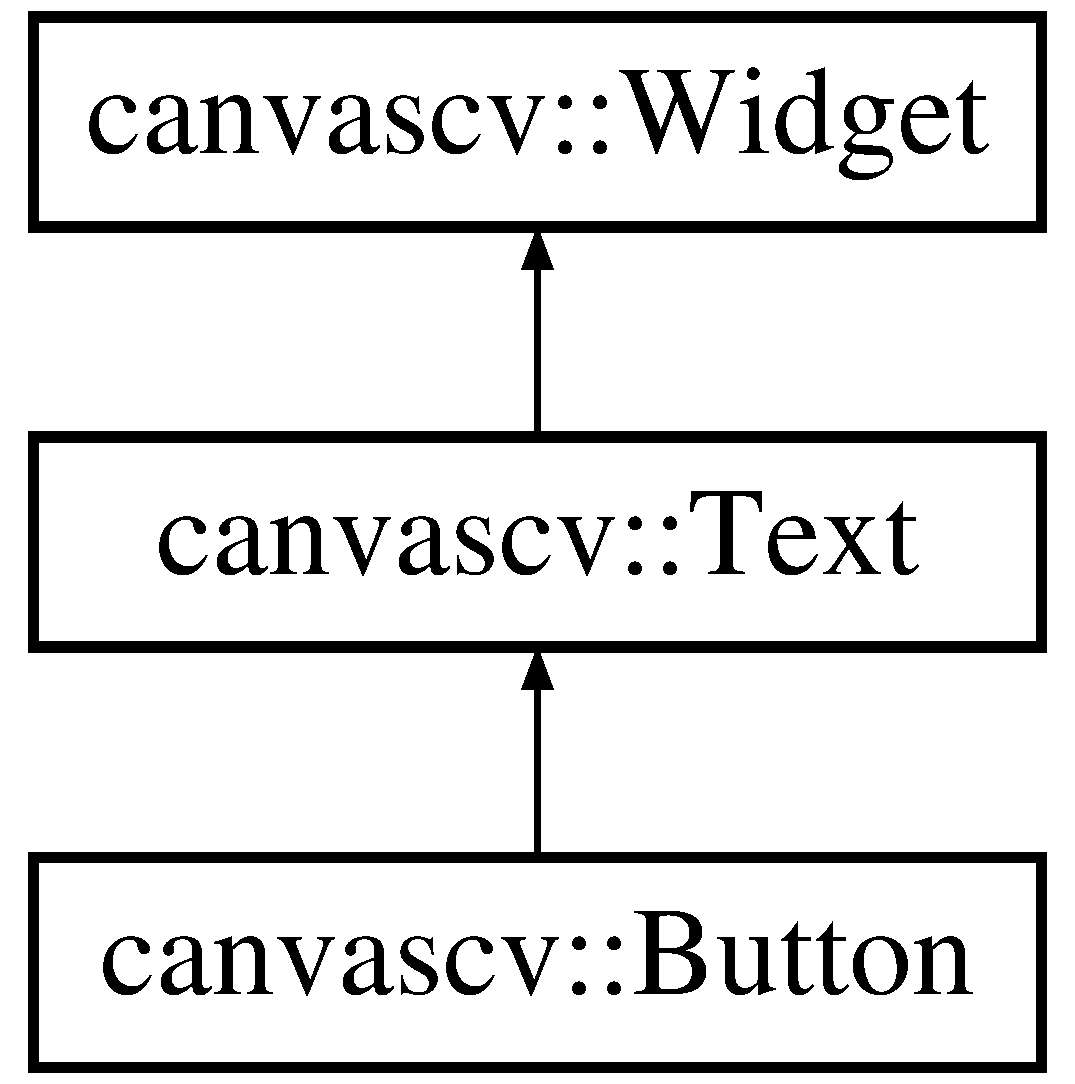
\includegraphics[height=3.000000cm]{classcanvascv_1_1Text}
\end{center}
\end{figure}
\subsection*{Public Member Functions}
\begin{DoxyCompactItemize}
\item 
virtual const char $\ast$ \hyperlink{classcanvascv_1_1Text_ae81d87d43167c2e8d1e58fa620a80579}{get\+Type} () const 
\begin{DoxyCompactList}\small\item\em get\+Type is always implemented by derived to return the same static pointer per widget. \end{DoxyCompactList}\item 
std\+::string \hyperlink{classcanvascv_1_1Text_acd9ec2f0271ac420775a029d84361581}{get\+Text} () const \hypertarget{classcanvascv_1_1Text_acd9ec2f0271ac420775a029d84361581}{}\label{classcanvascv_1_1Text_acd9ec2f0271ac420775a029d84361581}

\begin{DoxyCompactList}\small\item\em get the current text of the \hyperlink{classcanvascv_1_1Text}{Text} \end{DoxyCompactList}\item 
void \hyperlink{classcanvascv_1_1Text_aa54bad8c0b8eecdd5cd64138216ec83f}{set\+Text} (const std\+::string \&value)\hypertarget{classcanvascv_1_1Text_aa54bad8c0b8eecdd5cd64138216ec83f}{}\label{classcanvascv_1_1Text_aa54bad8c0b8eecdd5cd64138216ec83f}

\begin{DoxyCompactList}\small\item\em set the current text of the \hyperlink{classcanvascv_1_1Text}{Text} \end{DoxyCompactList}\item 
int \hyperlink{classcanvascv_1_1Text_ad535b8c794ff21380a7c9ccd7132d3ea}{get\+Font\+Face} () const \hypertarget{classcanvascv_1_1Text_ad535b8c794ff21380a7c9ccd7132d3ea}{}\label{classcanvascv_1_1Text_ad535b8c794ff21380a7c9ccd7132d3ea}

\begin{DoxyCompactList}\small\item\em get the Open\+CV font used \end{DoxyCompactList}\item 
void \hyperlink{classcanvascv_1_1Text_af0d610b5c5015df19befd15b3f600a4e}{set\+Font\+Face} (int value)\hypertarget{classcanvascv_1_1Text_af0d610b5c5015df19befd15b3f600a4e}{}\label{classcanvascv_1_1Text_af0d610b5c5015df19befd15b3f600a4e}

\begin{DoxyCompactList}\small\item\em set the Open\+CV font to use \end{DoxyCompactList}\item 
double \hyperlink{classcanvascv_1_1Text_a8af0c36c755f596b31cedf3043a51552}{get\+Font\+Scale} () const \hypertarget{classcanvascv_1_1Text_a8af0c36c755f596b31cedf3043a51552}{}\label{classcanvascv_1_1Text_a8af0c36c755f596b31cedf3043a51552}

\begin{DoxyCompactList}\small\item\em get the Open\+CV scale used for te font \end{DoxyCompactList}\item 
void \hyperlink{classcanvascv_1_1Text_a6541ae87e4577272feef0e30e1d5a24d}{set\+Font\+Scale} (double value)\hypertarget{classcanvascv_1_1Text_a6541ae87e4577272feef0e30e1d5a24d}{}\label{classcanvascv_1_1Text_a6541ae87e4577272feef0e30e1d5a24d}

\begin{DoxyCompactList}\small\item\em set the Open\+CV scale used for te font \end{DoxyCompactList}\item 
int \hyperlink{classcanvascv_1_1Text_ae314e7c415cc0b5aa7e56af8734fe526}{get\+Font\+Height} () const \hypertarget{classcanvascv_1_1Text_ae314e7c415cc0b5aa7e56af8734fe526}{}\label{classcanvascv_1_1Text_ae314e7c415cc0b5aa7e56af8734fe526}

\begin{DoxyCompactList}\small\item\em get the calculated font height (with padding and internal font spaces) \end{DoxyCompactList}\item 
void \hyperlink{classcanvascv_1_1Text_abb99c1a3328766b2079619db76de9f04}{set\+Font\+Height} (int value)\hypertarget{classcanvascv_1_1Text_abb99c1a3328766b2079619db76de9f04}{}\label{classcanvascv_1_1Text_abb99c1a3328766b2079619db76de9f04}

\begin{DoxyCompactList}\small\item\em set the font scale from a requested pixel height (with padding and internal font spaces) \end{DoxyCompactList}\item 
int \hyperlink{classcanvascv_1_1Text_a1c968ed06ba141eeeb99e3cc369988a3}{get\+Max\+Width} () const \hypertarget{classcanvascv_1_1Text_a1c968ed06ba141eeeb99e3cc369988a3}{}\label{classcanvascv_1_1Text_a1c968ed06ba141eeeb99e3cc369988a3}

\begin{DoxyCompactList}\small\item\em get the maxuimum allowed width of rows in pixels (0 means it\textquotesingle{}s disabled) \end{DoxyCompactList}\item 
void \hyperlink{classcanvascv_1_1Text_a6062c0756aceec5d6fe8f233173e4b03}{set\+Max\+Width} (int value)\hypertarget{classcanvascv_1_1Text_a6062c0756aceec5d6fe8f233173e4b03}{}\label{classcanvascv_1_1Text_a6062c0756aceec5d6fe8f233173e4b03}

\begin{DoxyCompactList}\small\item\em set the maxuimum allowed width of rows in pixels (0 to disable max width) \end{DoxyCompactList}\item 
virtual const cv\+::\+Rect \& \hyperlink{classcanvascv_1_1Text_a3b2c63327230c5763fe4262a804c41d0}{get\+Rect} ()\hypertarget{classcanvascv_1_1Text_a3b2c63327230c5763fe4262a804c41d0}{}\label{classcanvascv_1_1Text_a3b2c63327230c5763fe4262a804c41d0}

\begin{DoxyCompactList}\small\item\em Actual size the widget is occupying due to \hyperlink{classcanvascv_1_1Layout}{Layout} manager. \end{DoxyCompactList}\item 
virtual const cv\+::\+Rect \& \hyperlink{classcanvascv_1_1Text_a0cfed8ed9879101479795710dac4b1f2}{get\+Minimal\+Rect} ()\hypertarget{classcanvascv_1_1Text_a0cfed8ed9879101479795710dac4b1f2}{}\label{classcanvascv_1_1Text_a0cfed8ed9879101479795710dac4b1f2}

\begin{DoxyCompactList}\small\item\em Minimal size the widget coould have occupy. \end{DoxyCompactList}\item 
virtual void \hyperlink{classcanvascv_1_1Text_a94ccca8b1e03869a73699617a8c7f189}{recalc} ()\hypertarget{classcanvascv_1_1Text_a94ccca8b1e03869a73699617a8c7f189}{}\label{classcanvascv_1_1Text_a94ccca8b1e03869a73699617a8c7f189}

\begin{DoxyCompactList}\small\item\em update self so next call to \textquotesingle{}draw\textquotesingle{} will display correctly \end{DoxyCompactList}\item 
virtual void \hyperlink{classcanvascv_1_1Text_a2790e0fe1541df82c97879d393de687f}{draw\+FG} (cv\+::\+Mat \&dst)\hypertarget{classcanvascv_1_1Text_a2790e0fe1541df82c97879d393de687f}{}\label{classcanvascv_1_1Text_a2790e0fe1541df82c97879d393de687f}

\begin{DoxyCompactList}\small\item\em dst is the roi of the widget size and not the full image \end{DoxyCompactList}\end{DoxyCompactItemize}
\subsection*{Static Public Member Functions}
\begin{DoxyCompactItemize}
\item 
static std\+::shared\+\_\+ptr$<$ \hyperlink{classcanvascv_1_1Text}{Text} $>$ \hyperlink{classcanvascv_1_1Text_a7f3552263b6f185f78d90549e7ac38f7}{create} (\hyperlink{classcanvascv_1_1Layout}{Layout} \&layout, const cv\+::\+Point \&pos, const std\+::string \&text=\char`\"{}\char`\"{}, \hyperlink{classcanvascv_1_1Widget_a98ca3c300ba50b316fa5a1d300456abe}{Anchor} flow\+Anchor=\hyperlink{classcanvascv_1_1Widget_a98ca3c300ba50b316fa5a1d300456abeaa6a2c9d829ceed729afe8cb2f51b2f0c}{T\+OP}, \hyperlink{classcanvascv_1_1Widget_a98ca3c300ba50b316fa5a1d300456abe}{Anchor} layout\+Anchor=\hyperlink{classcanvascv_1_1Widget_a98ca3c300ba50b316fa5a1d300456abeaa6a2c9d829ceed729afe8cb2f51b2f0c}{T\+OP})
\begin{DoxyCompactList}\small\item\em create a \hyperlink{classcanvascv_1_1Text}{Text} widget \end{DoxyCompactList}\item 
static std\+::shared\+\_\+ptr$<$ \hyperlink{classcanvascv_1_1Text}{Text} $>$ \hyperlink{classcanvascv_1_1Text_ae95c6c8ba42111f81ce8120e9fe54fd6}{create} (\hyperlink{classcanvascv_1_1Layout}{Layout} \&layout, const std\+::string \&text=\char`\"{}\char`\"{}, \hyperlink{classcanvascv_1_1Widget_a98ca3c300ba50b316fa5a1d300456abe}{Anchor} flow\+Anchor=\hyperlink{classcanvascv_1_1Widget_a98ca3c300ba50b316fa5a1d300456abeaa6a2c9d829ceed729afe8cb2f51b2f0c}{T\+OP}, \hyperlink{classcanvascv_1_1Widget_a98ca3c300ba50b316fa5a1d300456abe}{Anchor} layout\+Anchor=\hyperlink{classcanvascv_1_1Widget_a98ca3c300ba50b316fa5a1d300456abeaa6a2c9d829ceed729afe8cb2f51b2f0c}{T\+OP})\hypertarget{classcanvascv_1_1Text_ae95c6c8ba42111f81ce8120e9fe54fd6}{}\label{classcanvascv_1_1Text_ae95c6c8ba42111f81ce8120e9fe54fd6}

\begin{DoxyCompactList}\small\item\em a convinient version to the above without the \textquotesingle{}pos\textquotesingle{} argument \end{DoxyCompactList}\end{DoxyCompactItemize}
\subsection*{Additional Inherited Members}


\subsection{Detailed Description}
Displaying text on the Open\+CV Window with/without a hilighting background. \begin{Desc}
\item[Examples\+: ]\par
\hyperlink{example_add_theme_8cpp-example}{example\+\_\+add\+\_\+theme.\+cpp}.\end{Desc}


\subsection{Member Function Documentation}
\index{canvascv\+::\+Text@{canvascv\+::\+Text}!create@{create}}
\index{create@{create}!canvascv\+::\+Text@{canvascv\+::\+Text}}
\subsubsection[{\texorpdfstring{create(\+Layout \&layout, const cv\+::\+Point \&pos, const std\+::string \&text="""", Anchor flow\+Anchor=\+T\+O\+P, Anchor layout\+Anchor=\+T\+O\+P)}{create(Layout &layout, const cv::Point &pos, const std::string &text="", Anchor flowAnchor=TOP, Anchor layoutAnchor=TOP)}}]{\setlength{\rightskip}{0pt plus 5cm}static std\+::shared\+\_\+ptr$<${\bf Text}$>$ canvascv\+::\+Text\+::create (
\begin{DoxyParamCaption}
\item[{{\bf Layout} \&}]{layout, }
\item[{const cv\+::\+Point \&}]{pos, }
\item[{const std\+::string \&}]{text = {\ttfamily \char`\"{}\char`\"{}}, }
\item[{{\bf Anchor}}]{flow\+Anchor = {\ttfamily {\bf T\+OP}}, }
\item[{{\bf Anchor}}]{layout\+Anchor = {\ttfamily {\bf T\+OP}}}
\end{DoxyParamCaption}
)\hspace{0.3cm}{\ttfamily [static]}}\hypertarget{classcanvascv_1_1Text_a7f3552263b6f185f78d90549e7ac38f7}{}\label{classcanvascv_1_1Text_a7f3552263b6f185f78d90549e7ac38f7}

\begin{DoxyParams}{Parameters}
{\em layout} & widgets are placed in layouts Canvas/\+V\+Frame/\+H\+Frame/... \\
\hline
{\em pos} & location in the \hyperlink{classcanvascv_1_1Layout}{Layout} (Layouts can ignore that) \\
\hline
{\em text} & what to write (accepts newline) \\
\hline
{\em flow\+Anchor} & affects the widget behavior
\begin{DoxyItemize}
\item T\+O\+P/\+B\+O\+T\+T\+OM -\/ text appears below or above pos
\item R\+I\+G\+H\+T/\+C\+E\+N\+T\+E\+R/\+L\+E\+FT is row alignment for multirows 
\end{DoxyItemize}\\
\hline
{\em layout\+Anchor} & affects the layout in the \hyperlink{classcanvascv_1_1Layout}{Layout} it belongs to
\begin{DoxyItemize}
\item T\+O\+P/\+C\+E\+N\+T\+E\+R/\+B\+O\+T\+T\+OM is relevat to a Horizontal\+Layout/\+H\+Frame (unless \hyperlink{classcanvascv_1_1Widget_a3ef50b76d33c332cea4e632346b6df33}{set\+Stretch\+Y()} is used)
\item R\+I\+G\+H\+T/\+C\+E\+N\+T\+E\+R/\+L\+E\+FT is relevat to a Vertical\+Layout/\+V\+Frame (unless \hyperlink{classcanvascv_1_1Widget_a7cdddebd755c499712793f727a057733}{set\+Stretch\+X()} is used) 
\end{DoxyItemize}\\
\hline
\end{DoxyParams}
\begin{DoxyReturn}{Returns}
a smart pointer copy of the object kept in the \hyperlink{classcanvascv_1_1Layout}{Layout} 
\end{DoxyReturn}
\begin{Desc}
\item[Examples\+: ]\par
\hyperlink{example_shapes_widgets_8cpp-example}{example\+\_\+shapes\+\_\+widgets.\+cpp}.\end{Desc}
\index{canvascv\+::\+Text@{canvascv\+::\+Text}!get\+Type@{get\+Type}}
\index{get\+Type@{get\+Type}!canvascv\+::\+Text@{canvascv\+::\+Text}}
\subsubsection[{\texorpdfstring{get\+Type() const }{getType() const }}]{\setlength{\rightskip}{0pt plus 5cm}virtual const char$\ast$ canvascv\+::\+Text\+::get\+Type (
\begin{DoxyParamCaption}
{}
\end{DoxyParamCaption}
) const\hspace{0.3cm}{\ttfamily [virtual]}}\hypertarget{classcanvascv_1_1Text_ae81d87d43167c2e8d1e58fa620a80579}{}\label{classcanvascv_1_1Text_ae81d87d43167c2e8d1e58fa620a80579}
\begin{DoxyReturn}{Returns}
const char $\ast$ pointer to string with widget type name 
\end{DoxyReturn}


Implements \hyperlink{classcanvascv_1_1Widget_a85884269bd53ab91203f099a586efa43}{canvascv\+::\+Widget}.



Reimplemented in \hyperlink{classcanvascv_1_1Button_ace294c72ce39507268ffd752f4ca0034}{canvascv\+::\+Button}.



The documentation for this class was generated from the following file\+:\begin{DoxyCompactItemize}
\item 
Canvas\+C\+V-\/doxygen/src/canvascv/widgets/text.\+h\end{DoxyCompactItemize}

\hypertarget{classcanvascv_1_1TextBox}{}\section{canvascv\+:\+:Text\+Box Class Reference}
\label{classcanvascv_1_1TextBox}\index{canvascv\+::\+Text\+Box@{canvascv\+::\+Text\+Box}}


The \hyperlink{classcanvascv_1_1TextBox}{Text\+Box} class.  




{\ttfamily \#include $<$textbox.\+h$>$}

Inheritance diagram for canvascv\+:\+:Text\+Box\+:\begin{figure}[H]
\begin{center}
\leavevmode
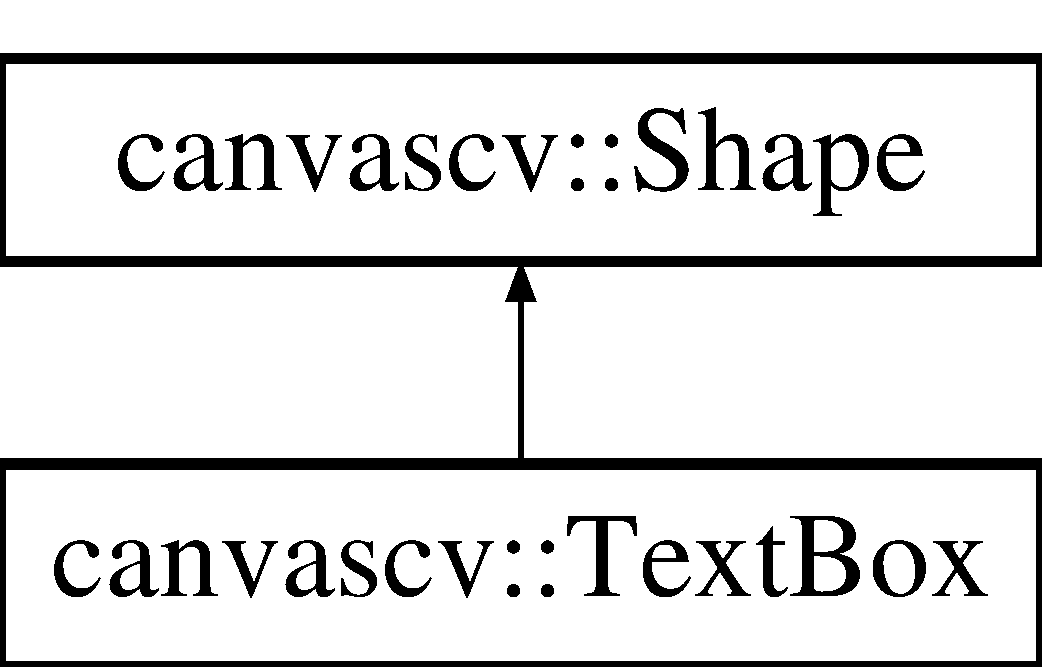
\includegraphics[height=2.000000cm]{classcanvascv_1_1TextBox}
\end{center}
\end{figure}
\subsection*{Public Member Functions}
\begin{DoxyCompactItemize}
\item 
const std\+::string \& \hyperlink{classcanvascv_1_1TextBox_a5e746210ed7911dc7a13751b38523b2f}{get\+Text} () const \hypertarget{classcanvascv_1_1TextBox_a5e746210ed7911dc7a13751b38523b2f}{}\label{classcanvascv_1_1TextBox_a5e746210ed7911dc7a13751b38523b2f}

\begin{DoxyCompactList}\small\item\em get the displayed text \end{DoxyCompactList}\item 
void \hyperlink{classcanvascv_1_1TextBox_a1470a20a5a732ac8bbed59b0fb88aaff}{set\+Text} (const std\+::string \&value)\hypertarget{classcanvascv_1_1TextBox_a1470a20a5a732ac8bbed59b0fb88aaff}{}\label{classcanvascv_1_1TextBox_a1470a20a5a732ac8bbed59b0fb88aaff}

\begin{DoxyCompactList}\small\item\em set the displayed text \end{DoxyCompactList}\item 
void \hyperlink{classcanvascv_1_1TextBox_ac948de159dd4f71fa9dfc686404386c5}{set\+TL} (const cv\+::\+Point \&value)\hypertarget{classcanvascv_1_1TextBox_ac948de159dd4f71fa9dfc686404386c5}{}\label{classcanvascv_1_1TextBox_ac948de159dd4f71fa9dfc686404386c5}

\begin{DoxyCompactList}\small\item\em set position (top left corner) \end{DoxyCompactList}\item 
int \hyperlink{classcanvascv_1_1TextBox_aa03df359a084e01741d6e67b16d6cb72}{get\+Font\+Face} () const \hypertarget{classcanvascv_1_1TextBox_aa03df359a084e01741d6e67b16d6cb72}{}\label{classcanvascv_1_1TextBox_aa03df359a084e01741d6e67b16d6cb72}

\begin{DoxyCompactList}\small\item\em get the font used \end{DoxyCompactList}\item 
void \hyperlink{classcanvascv_1_1TextBox_a12f81ba55169d9b611aed33e7a9d4267}{set\+Font\+Face} (int value)\hypertarget{classcanvascv_1_1TextBox_a12f81ba55169d9b611aed33e7a9d4267}{}\label{classcanvascv_1_1TextBox_a12f81ba55169d9b611aed33e7a9d4267}

\begin{DoxyCompactList}\small\item\em set the font used \end{DoxyCompactList}\item 
double \hyperlink{classcanvascv_1_1TextBox_a595171e5ca66b59554abc2cb930ad552}{get\+Font\+Scale} () const \hypertarget{classcanvascv_1_1TextBox_a595171e5ca66b59554abc2cb930ad552}{}\label{classcanvascv_1_1TextBox_a595171e5ca66b59554abc2cb930ad552}

\begin{DoxyCompactList}\small\item\em get the scale of the used font \end{DoxyCompactList}\item 
void \hyperlink{classcanvascv_1_1TextBox_a78870590353009cf8ef0bfd3cc05bb40}{set\+Font\+Scale} (double value)\hypertarget{classcanvascv_1_1TextBox_a78870590353009cf8ef0bfd3cc05bb40}{}\label{classcanvascv_1_1TextBox_a78870590353009cf8ef0bfd3cc05bb40}

\begin{DoxyCompactList}\small\item\em set the scale of the used font \end{DoxyCompactList}\item 
int \hyperlink{classcanvascv_1_1TextBox_a93bc214a13898e00d31ff2ddd2554c67}{get\+Font\+Thickness} () const \hypertarget{classcanvascv_1_1TextBox_a93bc214a13898e00d31ff2ddd2554c67}{}\label{classcanvascv_1_1TextBox_a93bc214a13898e00d31ff2ddd2554c67}

\begin{DoxyCompactList}\small\item\em get the thickness of the font \end{DoxyCompactList}\item 
void \hyperlink{classcanvascv_1_1TextBox_a0aea70368d5e4cf38a8e85177c612675}{set\+Font\+Thickness} (int value)\hypertarget{classcanvascv_1_1TextBox_a0aea70368d5e4cf38a8e85177c612675}{}\label{classcanvascv_1_1TextBox_a0aea70368d5e4cf38a8e85177c612675}

\begin{DoxyCompactList}\small\item\em set the thickness of the font \end{DoxyCompactList}\item 
cv\+::\+Scalar \hyperlink{classcanvascv_1_1TextBox_a9ff97837579ca91fe7266a86dffe35dd}{get\+Font\+Color} () const \hypertarget{classcanvascv_1_1TextBox_a9ff97837579ca91fe7266a86dffe35dd}{}\label{classcanvascv_1_1TextBox_a9ff97837579ca91fe7266a86dffe35dd}

\begin{DoxyCompactList}\small\item\em get the font color \end{DoxyCompactList}\item 
void \hyperlink{classcanvascv_1_1TextBox_ac2afa4502f04041000cd574fffaedcb4}{set\+Font\+Color} (const cv\+::\+Scalar \&value)\hypertarget{classcanvascv_1_1TextBox_ac2afa4502f04041000cd574fffaedcb4}{}\label{classcanvascv_1_1TextBox_ac2afa4502f04041000cd574fffaedcb4}

\begin{DoxyCompactList}\small\item\em set the font color \end{DoxyCompactList}\item 
virtual bool \hyperlink{classcanvascv_1_1TextBox_ab2545275695758bcd99c85560299bed8}{is\+At\+Pos} (const cv\+::\+Point \&pos)\hypertarget{classcanvascv_1_1TextBox_ab2545275695758bcd99c85560299bed8}{}\label{classcanvascv_1_1TextBox_ab2545275695758bcd99c85560299bed8}

\begin{DoxyCompactList}\small\item\em returns true if shape is at pos, false otherwise \end{DoxyCompactList}\item 
virtual std\+::list$<$ \hyperlink{classcanvascv_1_1Handle}{Handle} $\ast$ $>$ \hyperlink{classcanvascv_1_1TextBox_aef1fa0cd32292635c1b92b6ecd8b4aad}{get\+Connection\+Targets} ()
\begin{DoxyCompactList}\small\item\em get\+Connection\+Targets \end{DoxyCompactList}\item 
virtual std\+::shared\+\_\+ptr$<$ \hyperlink{classcanvascv_1_1Shape}{Shape} $>$ \hyperlink{classcanvascv_1_1TextBox_a100b59e6be1b9f9290e03654061c0ec1}{get\+Shape} (int id)
\begin{DoxyCompactList}\small\item\em get\+Shape \end{DoxyCompactList}\item 
virtual const char $\ast$ \hyperlink{classcanvascv_1_1TextBox_aa9313765c2040647a8fc32d227139c4d}{get\+Type} () const 
\begin{DoxyCompactList}\small\item\em get\+Type is always implemented by derived to return the same static pointer per shape. \end{DoxyCompactList}\end{DoxyCompactItemize}
\subsection*{Protected Member Functions}
\begin{DoxyCompactItemize}
\item 
virtual void \hyperlink{classcanvascv_1_1TextBox_a81bf5e2f8c85a805dfff4a401addd0bf}{draw} (cv\+::\+Mat \&canvas)
\begin{DoxyCompactList}\small\item\em draw shape on the canvas \end{DoxyCompactList}\item 
virtual bool \hyperlink{classcanvascv_1_1TextBox_adaf9422ce68a31eda4fc683ee0b74b8a}{mouse\+Pressed} (const cv\+::\+Point \&pos, bool on\+Create=false)
\begin{DoxyCompactList}\small\item\em mouse\+Pressed \end{DoxyCompactList}\item 
virtual bool \hyperlink{classcanvascv_1_1TextBox_a019cfc3fe096a51c65cc871d4e8be0b7}{mouse\+Moved} (const cv\+::\+Point \&pos)
\begin{DoxyCompactList}\small\item\em mouse\+Moved \end{DoxyCompactList}\item 
virtual bool \hyperlink{classcanvascv_1_1TextBox_ad048ee21fc55f500c6c85755d2d87aeb}{mouse\+Released} (const cv\+::\+Point \&pos)
\begin{DoxyCompactList}\small\item\em mouse\+Released \end{DoxyCompactList}\item 
virtual bool \hyperlink{classcanvascv_1_1TextBox_a4b9a7ecf58369f2161382d3c791542d7}{key\+Pressed} (int \&key)
\begin{DoxyCompactList}\small\item\em key\+Pressed will be called by \hyperlink{classcanvascv_1_1Canvas}{Canvas} for active shapes \end{DoxyCompactList}\item 
virtual void \hyperlink{classcanvascv_1_1TextBox_ab0dcb247e1aacf6d66879069d48975cd}{lost\+Focus} ()\hypertarget{classcanvascv_1_1TextBox_ab0dcb247e1aacf6d66879069d48975cd}{}\label{classcanvascv_1_1TextBox_ab0dcb247e1aacf6d66879069d48975cd}

\begin{DoxyCompactList}\small\item\em lost\+Focus is called by \hyperlink{classcanvascv_1_1Canvas}{Canvas} if we\textquotesingle{}re in it and just became non-\/active \end{DoxyCompactList}\end{DoxyCompactItemize}
\subsection*{Additional Inherited Members}


\subsection{Detailed Description}
Allows you to draw a line by mouse or from code \begin{Desc}
\item[Examples\+: ]\par
\hyperlink{example_shapes_widgets_8cpp-example}{example\+\_\+shapes\+\_\+widgets.\+cpp}.\end{Desc}


\subsection{Member Function Documentation}
\index{canvascv\+::\+Text\+Box@{canvascv\+::\+Text\+Box}!draw@{draw}}
\index{draw@{draw}!canvascv\+::\+Text\+Box@{canvascv\+::\+Text\+Box}}
\subsubsection[{\texorpdfstring{draw(cv\+::\+Mat \&canvas)}{draw(cv::Mat &canvas)}}]{\setlength{\rightskip}{0pt plus 5cm}virtual void canvascv\+::\+Text\+Box\+::draw (
\begin{DoxyParamCaption}
\item[{cv\+::\+Mat \&}]{canvas}
\end{DoxyParamCaption}
)\hspace{0.3cm}{\ttfamily [protected]}, {\ttfamily [virtual]}}\hypertarget{classcanvascv_1_1TextBox_a81bf5e2f8c85a805dfff4a401addd0bf}{}\label{classcanvascv_1_1TextBox_a81bf5e2f8c85a805dfff4a401addd0bf}

\begin{DoxyParams}{Parameters}
{\em canvas} & \\
\hline
\end{DoxyParams}


Implements \hyperlink{classcanvascv_1_1Shape_ab064fdb03d0d94ce84bde0b76b9e62c0}{canvascv\+::\+Shape}.

\index{canvascv\+::\+Text\+Box@{canvascv\+::\+Text\+Box}!get\+Connection\+Targets@{get\+Connection\+Targets}}
\index{get\+Connection\+Targets@{get\+Connection\+Targets}!canvascv\+::\+Text\+Box@{canvascv\+::\+Text\+Box}}
\subsubsection[{\texorpdfstring{get\+Connection\+Targets()}{getConnectionTargets()}}]{\setlength{\rightskip}{0pt plus 5cm}virtual std\+::list$<${\bf Handle} $\ast$$>$ canvascv\+::\+Text\+Box\+::get\+Connection\+Targets (
\begin{DoxyParamCaption}
{}
\end{DoxyParamCaption}
)\hspace{0.3cm}{\ttfamily [virtual]}}\hypertarget{classcanvascv_1_1TextBox_aef1fa0cd32292635c1b92b6ecd8b4aad}{}\label{classcanvascv_1_1TextBox_aef1fa0cd32292635c1b92b6ecd8b4aad}
Return a list of Handles this shape allows to connect to from other shapes (mainly for \hyperlink{classcanvascv_1_1ShapesConnector}{Shapes\+Connector}) \begin{DoxyReturn}{Returns}
list of \hyperlink{classcanvascv_1_1Handle}{Handle} pointers we \hyperlink{classcanvascv_1_1ShapesConnector}{Shapes\+Connector} can use to connect 
\end{DoxyReturn}


Implements \hyperlink{classcanvascv_1_1Shape_a827822e17e24118e16fa932ac0e71cd2}{canvascv\+::\+Shape}.

\index{canvascv\+::\+Text\+Box@{canvascv\+::\+Text\+Box}!get\+Shape@{get\+Shape}}
\index{get\+Shape@{get\+Shape}!canvascv\+::\+Text\+Box@{canvascv\+::\+Text\+Box}}
\subsubsection[{\texorpdfstring{get\+Shape(int id)}{getShape(int id)}}]{\setlength{\rightskip}{0pt plus 5cm}virtual std\+::shared\+\_\+ptr$<${\bf Shape}$>$ canvascv\+::\+Text\+Box\+::get\+Shape (
\begin{DoxyParamCaption}
\item[{int}]{id}
\end{DoxyParamCaption}
)\hspace{0.3cm}{\ttfamily [virtual]}}\hypertarget{classcanvascv_1_1TextBox_a100b59e6be1b9f9290e03654061c0ec1}{}\label{classcanvascv_1_1TextBox_a100b59e6be1b9f9290e03654061c0ec1}
Get internal shapes, which \hyperlink{classcanvascv_1_1Canvas}{Canvas} doesn\textquotesingle{}t know of. 
\begin{DoxyParams}{Parameters}
{\em id} & \\
\hline
\end{DoxyParams}
\begin{DoxyReturn}{Returns}
internal sub shape with requested id 
\end{DoxyReturn}


Reimplemented from \hyperlink{classcanvascv_1_1Shape_a89e585b5a1099f5ce291ded14db7181d}{canvascv\+::\+Shape}.

\index{canvascv\+::\+Text\+Box@{canvascv\+::\+Text\+Box}!get\+Type@{get\+Type}}
\index{get\+Type@{get\+Type}!canvascv\+::\+Text\+Box@{canvascv\+::\+Text\+Box}}
\subsubsection[{\texorpdfstring{get\+Type() const }{getType() const }}]{\setlength{\rightskip}{0pt plus 5cm}virtual const char$\ast$ canvascv\+::\+Text\+Box\+::get\+Type (
\begin{DoxyParamCaption}
{}
\end{DoxyParamCaption}
) const\hspace{0.3cm}{\ttfamily [virtual]}}\hypertarget{classcanvascv_1_1TextBox_aa9313765c2040647a8fc32d227139c4d}{}\label{classcanvascv_1_1TextBox_aa9313765c2040647a8fc32d227139c4d}
\begin{DoxyReturn}{Returns}
const char $\ast$ pointer to string with shape type name 
\end{DoxyReturn}


Implements \hyperlink{classcanvascv_1_1Shape_adee3cc696c7e82b0d2946e7e667ddd46}{canvascv\+::\+Shape}.

\index{canvascv\+::\+Text\+Box@{canvascv\+::\+Text\+Box}!key\+Pressed@{key\+Pressed}}
\index{key\+Pressed@{key\+Pressed}!canvascv\+::\+Text\+Box@{canvascv\+::\+Text\+Box}}
\subsubsection[{\texorpdfstring{key\+Pressed(int \&key)}{keyPressed(int &key)}}]{\setlength{\rightskip}{0pt plus 5cm}virtual bool canvascv\+::\+Text\+Box\+::key\+Pressed (
\begin{DoxyParamCaption}
\item[{int \&}]{key}
\end{DoxyParamCaption}
)\hspace{0.3cm}{\ttfamily [protected]}, {\ttfamily [virtual]}}\hypertarget{classcanvascv_1_1TextBox_a4b9a7ecf58369f2161382d3c791542d7}{}\label{classcanvascv_1_1TextBox_a4b9a7ecf58369f2161382d3c791542d7}

\begin{DoxyParams}{Parameters}
{\em key} & was pressed. You must set it to -\/1 if you consumed it. \\
\hline
\end{DoxyParams}
\begin{DoxyReturn}{Returns}
true if we want to stay in focus and false otherwise 
\end{DoxyReturn}


Reimplemented from \hyperlink{classcanvascv_1_1Shape_a7419dc43b9be99010e2b3bb973efbd37}{canvascv\+::\+Shape}.

\index{canvascv\+::\+Text\+Box@{canvascv\+::\+Text\+Box}!mouse\+Moved@{mouse\+Moved}}
\index{mouse\+Moved@{mouse\+Moved}!canvascv\+::\+Text\+Box@{canvascv\+::\+Text\+Box}}
\subsubsection[{\texorpdfstring{mouse\+Moved(const cv\+::\+Point \&pos)}{mouseMoved(const cv::Point &pos)}}]{\setlength{\rightskip}{0pt plus 5cm}virtual bool canvascv\+::\+Text\+Box\+::mouse\+Moved (
\begin{DoxyParamCaption}
\item[{const cv\+::\+Point \&}]{pos}
\end{DoxyParamCaption}
)\hspace{0.3cm}{\ttfamily [protected]}, {\ttfamily [virtual]}}\hypertarget{classcanvascv_1_1TextBox_a019cfc3fe096a51c65cc871d4e8be0b7}{}\label{classcanvascv_1_1TextBox_a019cfc3fe096a51c65cc871d4e8be0b7}

\begin{DoxyEnumerate}
\item Was a mouse moved over this shape?
\item If shape is during edit, then these are the mouse position. 
\begin{DoxyParams}{Parameters}
{\em pos} & \\
\hline
\end{DoxyParams}
\begin{DoxyReturn}{Returns}
true if a mouse moved over this shape, or it is during edit. false otherwise. 
\end{DoxyReturn}

\end{DoxyEnumerate}

Implements \hyperlink{classcanvascv_1_1Shape_acc72c3f645927c135dbc589e2c8678d4}{canvascv\+::\+Shape}.

\index{canvascv\+::\+Text\+Box@{canvascv\+::\+Text\+Box}!mouse\+Pressed@{mouse\+Pressed}}
\index{mouse\+Pressed@{mouse\+Pressed}!canvascv\+::\+Text\+Box@{canvascv\+::\+Text\+Box}}
\subsubsection[{\texorpdfstring{mouse\+Pressed(const cv\+::\+Point \&pos, bool on\+Create=false)}{mousePressed(const cv::Point &pos, bool onCreate=false)}}]{\setlength{\rightskip}{0pt plus 5cm}virtual bool canvascv\+::\+Text\+Box\+::mouse\+Pressed (
\begin{DoxyParamCaption}
\item[{const cv\+::\+Point \&}]{pos, }
\item[{bool}]{on\+Create = {\ttfamily false}}
\end{DoxyParamCaption}
)\hspace{0.3cm}{\ttfamily [protected]}, {\ttfamily [virtual]}}\hypertarget{classcanvascv_1_1TextBox_adaf9422ce68a31eda4fc683ee0b74b8a}{}\label{classcanvascv_1_1TextBox_adaf9422ce68a31eda4fc683ee0b74b8a}

\begin{DoxyParams}{Parameters}
{\em pos} & \\
\hline
{\em on\+Create} & is true if this is the mouse press which cerated this shape \\
\hline
\end{DoxyParams}
\begin{DoxyReturn}{Returns}
true for keep in focus, false for leave focus 
\end{DoxyReturn}


Implements \hyperlink{classcanvascv_1_1Shape_aa332adef968829dd7744cb1f6a491879}{canvascv\+::\+Shape}.

\index{canvascv\+::\+Text\+Box@{canvascv\+::\+Text\+Box}!mouse\+Released@{mouse\+Released}}
\index{mouse\+Released@{mouse\+Released}!canvascv\+::\+Text\+Box@{canvascv\+::\+Text\+Box}}
\subsubsection[{\texorpdfstring{mouse\+Released(const cv\+::\+Point \&pos)}{mouseReleased(const cv::Point &pos)}}]{\setlength{\rightskip}{0pt plus 5cm}virtual bool canvascv\+::\+Text\+Box\+::mouse\+Released (
\begin{DoxyParamCaption}
\item[{const cv\+::\+Point \&}]{pos}
\end{DoxyParamCaption}
)\hspace{0.3cm}{\ttfamily [protected]}, {\ttfamily [virtual]}}\hypertarget{classcanvascv_1_1TextBox_ad048ee21fc55f500c6c85755d2d87aeb}{}\label{classcanvascv_1_1TextBox_ad048ee21fc55f500c6c85755d2d87aeb}

\begin{DoxyParams}{Parameters}
{\em pos} & \\
\hline
\end{DoxyParams}
\begin{DoxyReturn}{Returns}
true for keep in focus, false for leave focus 
\end{DoxyReturn}


Implements \hyperlink{classcanvascv_1_1Shape_a8cbe386ff880c9830c0e4a97b335abf0}{canvascv\+::\+Shape}.



The documentation for this class was generated from the following file\+:\begin{DoxyCompactItemize}
\item 
Canvas\+C\+V-\/doxygen/src/canvascv/shapes/textbox.\+h\end{DoxyCompactItemize}

\hypertarget{classcanvascv_1_1Theme}{}\section{canvascv\+:\+:Theme Class Reference}
\label{classcanvascv_1_1Theme}\index{canvascv\+::\+Theme@{canvascv\+::\+Theme}}


The \hyperlink{classcanvascv_1_1Theme}{Theme} controls appearance of widgets and shapes.  




{\ttfamily \#include $<$theme.\+h$>$}

Inheritance diagram for canvascv\+:\+:Theme\+:\begin{figure}[H]
\begin{center}
\leavevmode
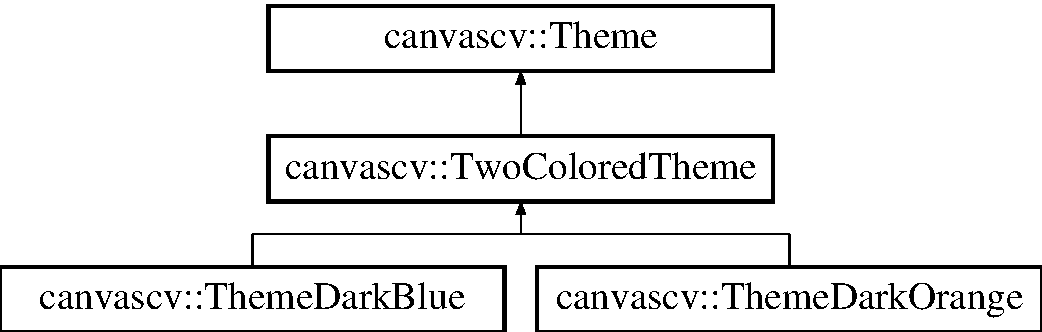
\includegraphics[height=3.000000cm]{classcanvascv_1_1Theme}
\end{center}
\end{figure}
\subsection*{Public Member Functions}
\begin{DoxyCompactItemize}
\item 
virtual void \hyperlink{classcanvascv_1_1Theme_a38ea37c836acfb37ee9b4d201c1f369b}{apply\+Style} (\hyperlink{classcanvascv_1_1Widget}{Widget} $\ast$widget)=0
\begin{DoxyCompactList}\small\item\em apply\+Style is called for every new widget created by the \hyperlink{classcanvascv_1_1WidgetFactory}{Widget\+Factory} \end{DoxyCompactList}\item 
virtual void \hyperlink{classcanvascv_1_1Theme_a0730fd4b881d57ee9d7b377238f8d24b}{apply\+Style} (\hyperlink{classcanvascv_1_1Shape}{Shape} $\ast$shape)=0
\begin{DoxyCompactList}\small\item\em apply\+Style is called for every new \hyperlink{classcanvascv_1_1Shape}{Shape} created by the \hyperlink{classcanvascv_1_1ShapeFactory}{Shape\+Factory} \end{DoxyCompactList}\item 
virtual void \hyperlink{classcanvascv_1_1Theme_a5f8c0e382d893419f9097bbc07e04130}{allocate\+BG} (cv\+::\+Mat \&dst, const cv\+::\+Size \&size, const cv\+::\+Scalar \&color)=0
\begin{DoxyCompactList}\small\item\em allocate\+BG creates the rect background for widgets \end{DoxyCompactList}\item 
virtual void \hyperlink{classcanvascv_1_1Theme_a2a7cbe4666031dcecfa50fa3dd1ec711}{flat} (cv\+::\+Mat \&bg, const cv\+::\+Scalar \&color)=0
\begin{DoxyCompactList}\small\item\em flat will cause bg to appear flat \end{DoxyCompactList}\item 
virtual void \hyperlink{classcanvascv_1_1Theme_ae23eaf232b60504c82fc46b59ccfee67}{raised} (cv\+::\+Mat \&bg, const cv\+::\+Scalar \&color)=0
\begin{DoxyCompactList}\small\item\em raised will cause bg to appear raised \end{DoxyCompactList}\item 
virtual void \hyperlink{classcanvascv_1_1Theme_a65ca2a83a09be3707304aeae3c53fd7e}{sunken} (cv\+::\+Mat \&bg, const cv\+::\+Scalar \&color)=0
\begin{DoxyCompactList}\small\item\em sunken will cause bg to appear sunken \end{DoxyCompactList}\item 
virtual void \hyperlink{classcanvascv_1_1Theme_aa92819f6a08112b5ff489b00f66a3ce0}{selected} (cv\+::\+Mat \&bg, const cv\+::\+Scalar \&color)=0
\begin{DoxyCompactList}\small\item\em selected will cause bg to appear selecte \end{DoxyCompactList}\end{DoxyCompactItemize}


\subsection{Detailed Description}
Themes are added to the \hyperlink{classcanvascv_1_1ThemeRepository}{Theme\+Repository}. You can add your own external themes. 

\subsection{Member Function Documentation}
\index{canvascv\+::\+Theme@{canvascv\+::\+Theme}!allocate\+BG@{allocate\+BG}}
\index{allocate\+BG@{allocate\+BG}!canvascv\+::\+Theme@{canvascv\+::\+Theme}}
\subsubsection[{\texorpdfstring{allocate\+B\+G(cv\+::\+Mat \&dst, const cv\+::\+Size \&size, const cv\+::\+Scalar \&color)=0}{allocateBG(cv::Mat &dst, const cv::Size &size, const cv::Scalar &color)=0}}]{\setlength{\rightskip}{0pt plus 5cm}virtual void canvascv\+::\+Theme\+::allocate\+BG (
\begin{DoxyParamCaption}
\item[{cv\+::\+Mat \&}]{dst, }
\item[{const cv\+::\+Size \&}]{size, }
\item[{const cv\+::\+Scalar \&}]{color}
\end{DoxyParamCaption}
)\hspace{0.3cm}{\ttfamily [pure virtual]}}\hypertarget{classcanvascv_1_1Theme_a5f8c0e382d893419f9097bbc07e04130}{}\label{classcanvascv_1_1Theme_a5f8c0e382d893419f9097bbc07e04130}

\begin{DoxyParams}{Parameters}
{\em dst} & is a Mat dedicated to hold the background will be filled with 4 channels \\
\hline
{\em size} & will be the size of dst when done \\
\hline
{\em color} & is the requested color, with alpha, which the theme is allowed to ignore \\
\hline
\end{DoxyParams}


Implemented in \hyperlink{classcanvascv_1_1TwoColoredTheme_ae085f9cd7f170e49fbc463348a4eb7b5}{canvascv\+::\+Two\+Colored\+Theme}.

\index{canvascv\+::\+Theme@{canvascv\+::\+Theme}!apply\+Style@{apply\+Style}}
\index{apply\+Style@{apply\+Style}!canvascv\+::\+Theme@{canvascv\+::\+Theme}}
\subsubsection[{\texorpdfstring{apply\+Style(\+Widget $\ast$widget)=0}{applyStyle(Widget *widget)=0}}]{\setlength{\rightskip}{0pt plus 5cm}virtual void canvascv\+::\+Theme\+::apply\+Style (
\begin{DoxyParamCaption}
\item[{{\bf Widget} $\ast$}]{widget}
\end{DoxyParamCaption}
)\hspace{0.3cm}{\ttfamily [pure virtual]}}\hypertarget{classcanvascv_1_1Theme_a38ea37c836acfb37ee9b4d201c1f369b}{}\label{classcanvascv_1_1Theme_a38ea37c836acfb37ee9b4d201c1f369b}

\begin{DoxyParams}{Parameters}
{\em widget} & will have setters invoked according to the theme \\
\hline
\end{DoxyParams}


Implemented in \hyperlink{classcanvascv_1_1TwoColoredTheme_a2a725588ca2e1c33900019622cc8fe9a}{canvascv\+::\+Two\+Colored\+Theme}.

\index{canvascv\+::\+Theme@{canvascv\+::\+Theme}!apply\+Style@{apply\+Style}}
\index{apply\+Style@{apply\+Style}!canvascv\+::\+Theme@{canvascv\+::\+Theme}}
\subsubsection[{\texorpdfstring{apply\+Style(\+Shape $\ast$shape)=0}{applyStyle(Shape *shape)=0}}]{\setlength{\rightskip}{0pt plus 5cm}virtual void canvascv\+::\+Theme\+::apply\+Style (
\begin{DoxyParamCaption}
\item[{{\bf Shape} $\ast$}]{shape}
\end{DoxyParamCaption}
)\hspace{0.3cm}{\ttfamily [pure virtual]}}\hypertarget{classcanvascv_1_1Theme_a0730fd4b881d57ee9d7b377238f8d24b}{}\label{classcanvascv_1_1Theme_a0730fd4b881d57ee9d7b377238f8d24b}

\begin{DoxyParams}{Parameters}
{\em shape} & will have setters invoked according to the theme \\
\hline
\end{DoxyParams}


Implemented in \hyperlink{classcanvascv_1_1TwoColoredTheme_ada225b2ed04e78caded01b23de343b1f}{canvascv\+::\+Two\+Colored\+Theme}.

\index{canvascv\+::\+Theme@{canvascv\+::\+Theme}!flat@{flat}}
\index{flat@{flat}!canvascv\+::\+Theme@{canvascv\+::\+Theme}}
\subsubsection[{\texorpdfstring{flat(cv\+::\+Mat \&bg, const cv\+::\+Scalar \&color)=0}{flat(cv::Mat &bg, const cv::Scalar &color)=0}}]{\setlength{\rightskip}{0pt plus 5cm}virtual void canvascv\+::\+Theme\+::flat (
\begin{DoxyParamCaption}
\item[{cv\+::\+Mat \&}]{bg, }
\item[{const cv\+::\+Scalar \&}]{color}
\end{DoxyParamCaption}
)\hspace{0.3cm}{\ttfamily [pure virtual]}}\hypertarget{classcanvascv_1_1Theme_a2a7cbe4666031dcecfa50fa3dd1ec711}{}\label{classcanvascv_1_1Theme_a2a7cbe4666031dcecfa50fa3dd1ec711}

\begin{DoxyParams}{Parameters}
{\em bg} & was previously allocated by \hyperlink{classcanvascv_1_1Theme_a5f8c0e382d893419f9097bbc07e04130}{allocate\+B\+G()} \\
\hline
{\em color} & could be used for drawing, but the theme is allowed to ignore it \\
\hline
\end{DoxyParams}


Implemented in \hyperlink{classcanvascv_1_1TwoColoredTheme_a76c1d4f249bb5d01ff07b4559cbdd592}{canvascv\+::\+Two\+Colored\+Theme}.

\index{canvascv\+::\+Theme@{canvascv\+::\+Theme}!raised@{raised}}
\index{raised@{raised}!canvascv\+::\+Theme@{canvascv\+::\+Theme}}
\subsubsection[{\texorpdfstring{raised(cv\+::\+Mat \&bg, const cv\+::\+Scalar \&color)=0}{raised(cv::Mat &bg, const cv::Scalar &color)=0}}]{\setlength{\rightskip}{0pt plus 5cm}virtual void canvascv\+::\+Theme\+::raised (
\begin{DoxyParamCaption}
\item[{cv\+::\+Mat \&}]{bg, }
\item[{const cv\+::\+Scalar \&}]{color}
\end{DoxyParamCaption}
)\hspace{0.3cm}{\ttfamily [pure virtual]}}\hypertarget{classcanvascv_1_1Theme_ae23eaf232b60504c82fc46b59ccfee67}{}\label{classcanvascv_1_1Theme_ae23eaf232b60504c82fc46b59ccfee67}

\begin{DoxyParams}{Parameters}
{\em bg} & was previously allocated by \hyperlink{classcanvascv_1_1Theme_a5f8c0e382d893419f9097bbc07e04130}{allocate\+B\+G()} \\
\hline
{\em color} & could be used for drawing, but the theme is allowed to ignore it \\
\hline
\end{DoxyParams}


Implemented in \hyperlink{classcanvascv_1_1TwoColoredTheme_a5c3d937a5e36e80eff6f7683f2898589}{canvascv\+::\+Two\+Colored\+Theme}.

\index{canvascv\+::\+Theme@{canvascv\+::\+Theme}!selected@{selected}}
\index{selected@{selected}!canvascv\+::\+Theme@{canvascv\+::\+Theme}}
\subsubsection[{\texorpdfstring{selected(cv\+::\+Mat \&bg, const cv\+::\+Scalar \&color)=0}{selected(cv::Mat &bg, const cv::Scalar &color)=0}}]{\setlength{\rightskip}{0pt plus 5cm}virtual void canvascv\+::\+Theme\+::selected (
\begin{DoxyParamCaption}
\item[{cv\+::\+Mat \&}]{bg, }
\item[{const cv\+::\+Scalar \&}]{color}
\end{DoxyParamCaption}
)\hspace{0.3cm}{\ttfamily [pure virtual]}}\hypertarget{classcanvascv_1_1Theme_aa92819f6a08112b5ff489b00f66a3ce0}{}\label{classcanvascv_1_1Theme_aa92819f6a08112b5ff489b00f66a3ce0}

\begin{DoxyParams}{Parameters}
{\em bg} & was previously allocated by \hyperlink{classcanvascv_1_1Theme_a5f8c0e382d893419f9097bbc07e04130}{allocate\+B\+G()} \\
\hline
{\em color} & could be used for drawing, but the theme is allowed to ignore it \\
\hline
\end{DoxyParams}


Implemented in \hyperlink{classcanvascv_1_1TwoColoredTheme_abee098f6af5b63fa06441184c2c331bb}{canvascv\+::\+Two\+Colored\+Theme}.

\index{canvascv\+::\+Theme@{canvascv\+::\+Theme}!sunken@{sunken}}
\index{sunken@{sunken}!canvascv\+::\+Theme@{canvascv\+::\+Theme}}
\subsubsection[{\texorpdfstring{sunken(cv\+::\+Mat \&bg, const cv\+::\+Scalar \&color)=0}{sunken(cv::Mat &bg, const cv::Scalar &color)=0}}]{\setlength{\rightskip}{0pt plus 5cm}virtual void canvascv\+::\+Theme\+::sunken (
\begin{DoxyParamCaption}
\item[{cv\+::\+Mat \&}]{bg, }
\item[{const cv\+::\+Scalar \&}]{color}
\end{DoxyParamCaption}
)\hspace{0.3cm}{\ttfamily [pure virtual]}}\hypertarget{classcanvascv_1_1Theme_a65ca2a83a09be3707304aeae3c53fd7e}{}\label{classcanvascv_1_1Theme_a65ca2a83a09be3707304aeae3c53fd7e}

\begin{DoxyParams}{Parameters}
{\em bg} & was previously allocated by \hyperlink{classcanvascv_1_1Theme_a5f8c0e382d893419f9097bbc07e04130}{allocate\+B\+G()} \\
\hline
{\em color} & could be used for drawing, but the theme is allowed to ignore it \\
\hline
\end{DoxyParams}


Implemented in \hyperlink{classcanvascv_1_1TwoColoredTheme_a2b39a62e7aa5836b9957d1c8257167c3}{canvascv\+::\+Two\+Colored\+Theme}.



The documentation for this class was generated from the following file\+:\begin{DoxyCompactItemize}
\item 
Canvas\+C\+V-\/doxygen/src/canvascv/themes/theme.\+h\end{DoxyCompactItemize}

\hypertarget{classcanvascv_1_1ThemeDarkBlue}{}\section{canvascv\+:\+:Theme\+Dark\+Blue Class Reference}
\label{classcanvascv_1_1ThemeDarkBlue}\index{canvascv\+::\+Theme\+Dark\+Blue@{canvascv\+::\+Theme\+Dark\+Blue}}


The \hyperlink{classcanvascv_1_1ThemeDarkBlue}{Theme\+Dark\+Blue} class implements a dark theme of blue over dark gray colors.  




{\ttfamily \#include $<$themedarkblue.\+h$>$}

Inheritance diagram for canvascv\+:\+:Theme\+Dark\+Blue\+:\begin{figure}[H]
\begin{center}
\leavevmode
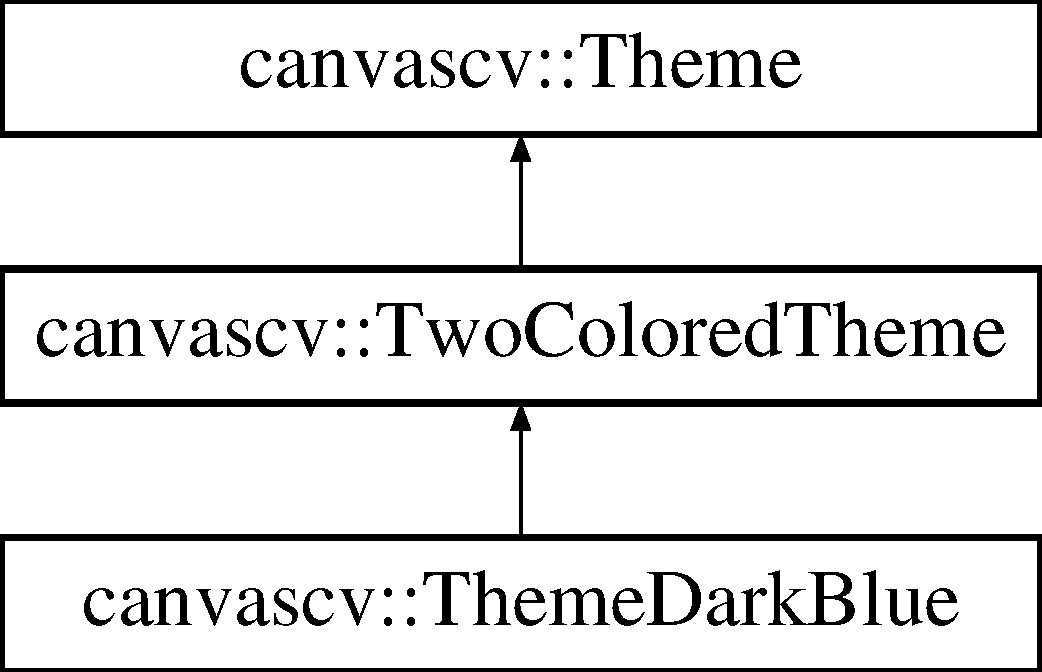
\includegraphics[height=3.000000cm]{classcanvascv_1_1ThemeDarkBlue}
\end{center}
\end{figure}
\subsection*{Additional Inherited Members}


The documentation for this class was generated from the following file\+:\begin{DoxyCompactItemize}
\item 
Canvas\+C\+V-\/doxygen/src/canvascv/themes/themedarkblue.\+h\end{DoxyCompactItemize}

\hypertarget{classcanvascv_1_1ThemeDarkOrange}{}\section{canvascv\+:\+:Theme\+Dark\+Orange Class Reference}
\label{classcanvascv_1_1ThemeDarkOrange}\index{canvascv\+::\+Theme\+Dark\+Orange@{canvascv\+::\+Theme\+Dark\+Orange}}


The \hyperlink{classcanvascv_1_1ThemeDarkOrange}{Theme\+Dark\+Orange} class implements a dark theme of orange over dark gray colors.  




{\ttfamily \#include $<$themedarkorange.\+h$>$}

Inheritance diagram for canvascv\+:\+:Theme\+Dark\+Orange\+:\begin{figure}[H]
\begin{center}
\leavevmode
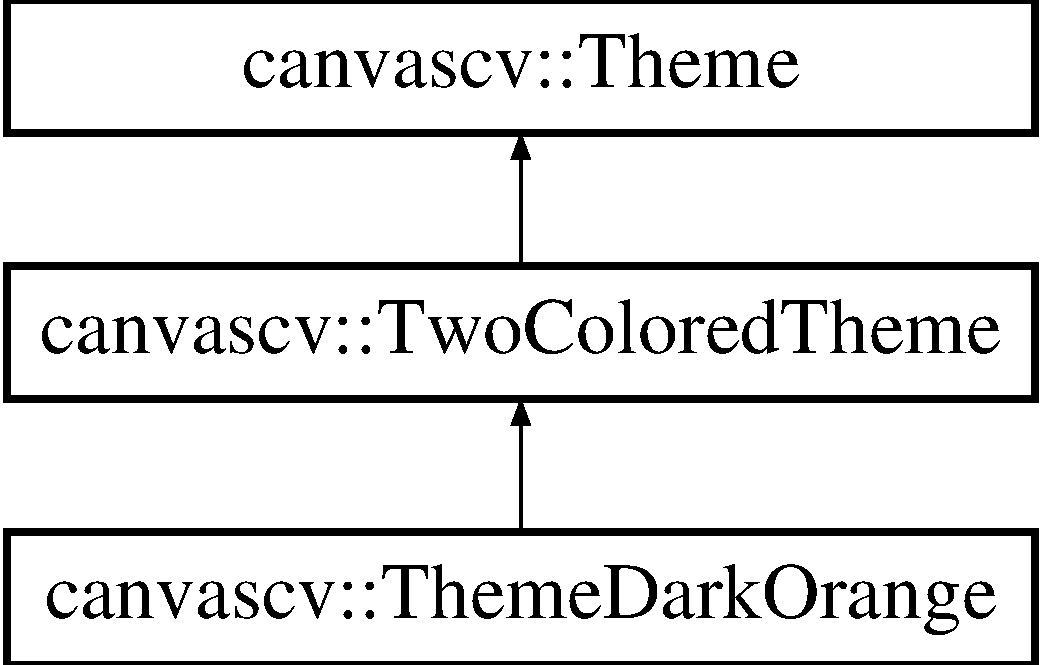
\includegraphics[height=3.000000cm]{classcanvascv_1_1ThemeDarkOrange}
\end{center}
\end{figure}
\subsection*{Additional Inherited Members}


The documentation for this class was generated from the following file\+:\begin{DoxyCompactItemize}
\item 
Canvas\+C\+V-\/doxygen/src/canvascv/themes/themedarkorange.\+h\end{DoxyCompactItemize}

\hypertarget{classcanvascv_1_1ThemeRepository}{}\section{canvascv\+:\+:Theme\+Repository Class Reference}
\label{classcanvascv_1_1ThemeRepository}\index{canvascv\+::\+Theme\+Repository@{canvascv\+::\+Theme\+Repository}}


The \hyperlink{classcanvascv_1_1ThemeRepository}{Theme\+Repository} is used to add and get themes for \hyperlink{classcanvascv_1_1Widget}{Widget} and \hyperlink{classcanvascv_1_1Shape}{Shape} objects.  




{\ttfamily \#include $<$themerepository.\+h$>$}

\subsection*{Static Public Member Functions}
\begin{DoxyCompactItemize}
\item 
static bool \hyperlink{classcanvascv_1_1ThemeRepository_ac4c17001de8990373066ee3cc9c8a167}{add\+Theme} (const std\+::string \&name, \hyperlink{classcanvascv_1_1Theme}{Theme} $\ast$theme)
\begin{DoxyCompactList}\small\item\em add\+Theme add a \hyperlink{classcanvascv_1_1Theme}{Theme} to the repository \end{DoxyCompactList}\item 
static void \hyperlink{classcanvascv_1_1ThemeRepository_a0adfc9060f4c9f274e3be5800b952a8f}{set\+Current\+Theme} (const std\+::string \&name)
\begin{DoxyCompactList}\small\item\em set\+Current\+Theme sets a previously added theme \end{DoxyCompactList}\item 
static \hyperlink{classcanvascv_1_1Theme}{Theme} $\ast$ \hyperlink{classcanvascv_1_1ThemeRepository_af63c1f2e5bac4f6adbaa328234aa476d}{get\+Current\+Theme} ()\hypertarget{classcanvascv_1_1ThemeRepository_af63c1f2e5bac4f6adbaa328234aa476d}{}\label{classcanvascv_1_1ThemeRepository_af63c1f2e5bac4f6adbaa328234aa476d}

\begin{DoxyCompactList}\small\item\em returns the current theme \end{DoxyCompactList}\item 
static std\+::string \hyperlink{classcanvascv_1_1ThemeRepository_a5cbfe3483cb442b3317f2d6dff983966}{get\+Current\+Theme\+Name} ()\hypertarget{classcanvascv_1_1ThemeRepository_a5cbfe3483cb442b3317f2d6dff983966}{}\label{classcanvascv_1_1ThemeRepository_a5cbfe3483cb442b3317f2d6dff983966}

\begin{DoxyCompactList}\small\item\em returns the current theme name \end{DoxyCompactList}\item 
static void \hyperlink{classcanvascv_1_1ThemeRepository_af64bf9462b980772c4c8c11132edec26}{apply\+Current\+Theme} (\hyperlink{classcanvascv_1_1Shape}{Shape} $\ast$shape)\hypertarget{classcanvascv_1_1ThemeRepository_af64bf9462b980772c4c8c11132edec26}{}\label{classcanvascv_1_1ThemeRepository_af64bf9462b980772c4c8c11132edec26}

\begin{DoxyCompactList}\small\item\em used automatically by the \hyperlink{classcanvascv_1_1ShapeFactory}{Shape\+Factory} when creating a shape \end{DoxyCompactList}\item 
static void \hyperlink{classcanvascv_1_1ThemeRepository_a92d582b9eef45fabdd2ff6dc354250cf}{apply\+Current\+Theme} (\hyperlink{classcanvascv_1_1Widget}{Widget} $\ast$widget)\hypertarget{classcanvascv_1_1ThemeRepository_a92d582b9eef45fabdd2ff6dc354250cf}{}\label{classcanvascv_1_1ThemeRepository_a92d582b9eef45fabdd2ff6dc354250cf}

\begin{DoxyCompactList}\small\item\em used automatically by the \hyperlink{classcanvascv_1_1WidgetFactory}{Widget\+Factory} when creating a widget \end{DoxyCompactList}\item 
static std\+::vector$<$ std\+::string $>$ \hyperlink{classcanvascv_1_1ThemeRepository_aec4b1a6a992907e16da57fde49e4b861}{avail\+Themes} ()\hypertarget{classcanvascv_1_1ThemeRepository_aec4b1a6a992907e16da57fde49e4b861}{}\label{classcanvascv_1_1ThemeRepository_aec4b1a6a992907e16da57fde49e4b861}

\begin{DoxyCompactList}\small\item\em get a list of available theme names \end{DoxyCompactList}\end{DoxyCompactItemize}


\subsection{Detailed Description}
This class must have at least a single theme. Themes can be a part of this library, or external to it, suplied by the user and added with \hyperlink{classcanvascv_1_1ThemeRepository_ac4c17001de8990373066ee3cc9c8a167}{Theme\+Repository\+::add\+Theme()} 

\subsection{Member Function Documentation}
\index{canvascv\+::\+Theme\+Repository@{canvascv\+::\+Theme\+Repository}!add\+Theme@{add\+Theme}}
\index{add\+Theme@{add\+Theme}!canvascv\+::\+Theme\+Repository@{canvascv\+::\+Theme\+Repository}}
\subsubsection[{\texorpdfstring{add\+Theme(const std\+::string \&name, Theme $\ast$theme)}{addTheme(const std::string &name, Theme *theme)}}]{\setlength{\rightskip}{0pt plus 5cm}static bool canvascv\+::\+Theme\+Repository\+::add\+Theme (
\begin{DoxyParamCaption}
\item[{const std\+::string \&}]{name, }
\item[{{\bf Theme} $\ast$}]{theme}
\end{DoxyParamCaption}
)\hspace{0.3cm}{\ttfamily [static]}}\hypertarget{classcanvascv_1_1ThemeRepository_ac4c17001de8990373066ee3cc9c8a167}{}\label{classcanvascv_1_1ThemeRepository_ac4c17001de8990373066ee3cc9c8a167}

\begin{DoxyParams}{Parameters}
{\em name} & is the name of the theme (to overide a theme, add something instead with the same name) \\
\hline
{\em theme} & is the theme associated with this name \\
\hline
\end{DoxyParams}
\begin{DoxyReturn}{Returns}
true if theme is not null 
\end{DoxyReturn}
\begin{DoxyNote}{Note}
that you cannot delete the \hyperlink{classcanvascv_1_1Theme}{Theme} pointer while it\textquotesingle{}s in use. 
\end{DoxyNote}
\begin{DoxySeeAlso}{See also}
\hyperlink{classcanvascv_1_1ThemeRepository_a0adfc9060f4c9f274e3be5800b952a8f}{set\+Current\+Theme()} 
\end{DoxySeeAlso}
\index{canvascv\+::\+Theme\+Repository@{canvascv\+::\+Theme\+Repository}!set\+Current\+Theme@{set\+Current\+Theme}}
\index{set\+Current\+Theme@{set\+Current\+Theme}!canvascv\+::\+Theme\+Repository@{canvascv\+::\+Theme\+Repository}}
\subsubsection[{\texorpdfstring{set\+Current\+Theme(const std\+::string \&name)}{setCurrentTheme(const std::string &name)}}]{\setlength{\rightskip}{0pt plus 5cm}static void canvascv\+::\+Theme\+Repository\+::set\+Current\+Theme (
\begin{DoxyParamCaption}
\item[{const std\+::string \&}]{name}
\end{DoxyParamCaption}
)\hspace{0.3cm}{\ttfamily [static]}}\hypertarget{classcanvascv_1_1ThemeRepository_a0adfc9060f4c9f274e3be5800b952a8f}{}\label{classcanvascv_1_1ThemeRepository_a0adfc9060f4c9f274e3be5800b952a8f}

\begin{DoxyParams}{Parameters}
{\em name} & is the name of the \hyperlink{classcanvascv_1_1Theme}{Theme} to set as default \\
\hline
\end{DoxyParams}
\begin{DoxyNote}{Note}
if the theme doesn\textquotesingle{}t exist then nothing happens 
\end{DoxyNote}


The documentation for this class was generated from the following file\+:\begin{DoxyCompactItemize}
\item 
Canvas\+C\+V-\/doxygen/src/canvascv/themes/themerepository.\+h\end{DoxyCompactItemize}

\hypertarget{classcanvascv_1_1TwoColoredTheme}{}\section{canvascv\+:\+:Two\+Colored\+Theme Class Reference}
\label{classcanvascv_1_1TwoColoredTheme}\index{canvascv\+::\+Two\+Colored\+Theme@{canvascv\+::\+Two\+Colored\+Theme}}


The Theme\+Dark class implements a 2 colored theme base class.  




{\ttfamily \#include $<$twocoloredtheme.\+h$>$}

Inheritance diagram for canvascv\+:\+:Two\+Colored\+Theme\+:\begin{figure}[H]
\begin{center}
\leavevmode
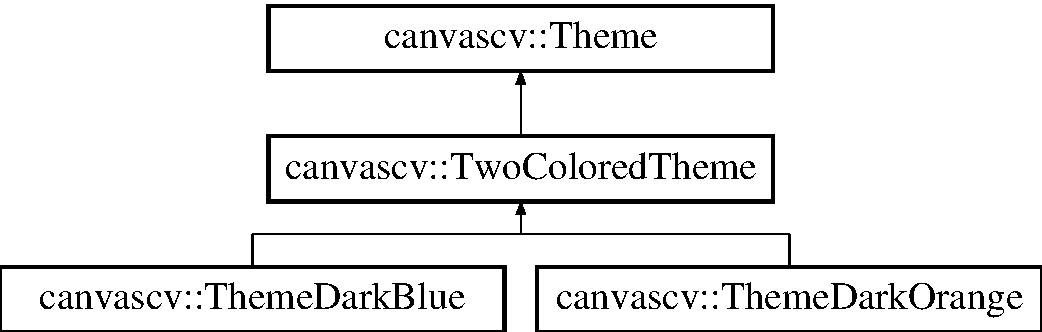
\includegraphics[height=3.000000cm]{classcanvascv_1_1TwoColoredTheme}
\end{center}
\end{figure}
\subsection*{Public Member Functions}
\begin{DoxyCompactItemize}
\item 
virtual void \hyperlink{classcanvascv_1_1TwoColoredTheme_a2a725588ca2e1c33900019622cc8fe9a}{apply\+Style} (\hyperlink{classcanvascv_1_1Widget}{Widget} $\ast$widget)
\begin{DoxyCompactList}\small\item\em apply\+Style is called for every new widget created by the \hyperlink{classcanvascv_1_1WidgetFactory}{Widget\+Factory} \end{DoxyCompactList}\item 
virtual void \hyperlink{classcanvascv_1_1TwoColoredTheme_ada225b2ed04e78caded01b23de343b1f}{apply\+Style} (\hyperlink{classcanvascv_1_1Shape}{Shape} $\ast$shape)
\begin{DoxyCompactList}\small\item\em apply\+Style is called for every new \hyperlink{classcanvascv_1_1Shape}{Shape} created by the \hyperlink{classcanvascv_1_1ShapeFactory}{Shape\+Factory} \end{DoxyCompactList}\item 
virtual void \hyperlink{classcanvascv_1_1TwoColoredTheme_ae085f9cd7f170e49fbc463348a4eb7b5}{allocate\+BG} (cv\+::\+Mat \&dst, const cv\+::\+Size \&size, const cv\+::\+Scalar \&color)
\begin{DoxyCompactList}\small\item\em allocate\+BG creates the rect background for widgets \end{DoxyCompactList}\item 
virtual void \hyperlink{classcanvascv_1_1TwoColoredTheme_a76c1d4f249bb5d01ff07b4559cbdd592}{flat} (cv\+::\+Mat \&bg, const cv\+::\+Scalar \&color)
\begin{DoxyCompactList}\small\item\em flat will cause bg to appear flat \end{DoxyCompactList}\item 
virtual void \hyperlink{classcanvascv_1_1TwoColoredTheme_a5c3d937a5e36e80eff6f7683f2898589}{raised} (cv\+::\+Mat \&bg, const cv\+::\+Scalar \&color)
\begin{DoxyCompactList}\small\item\em raised will cause bg to appear raised \end{DoxyCompactList}\item 
virtual void \hyperlink{classcanvascv_1_1TwoColoredTheme_a2b39a62e7aa5836b9957d1c8257167c3}{sunken} (cv\+::\+Mat \&bg, const cv\+::\+Scalar \&color)
\begin{DoxyCompactList}\small\item\em sunken will cause bg to appear sunken \end{DoxyCompactList}\item 
virtual void \hyperlink{classcanvascv_1_1TwoColoredTheme_abee098f6af5b63fa06441184c2c331bb}{selected} (cv\+::\+Mat \&bg, const cv\+::\+Scalar \&color)
\begin{DoxyCompactList}\small\item\em selected will cause bg to appear selecte \end{DoxyCompactList}\end{DoxyCompactItemize}


\subsection{Detailed Description}
\begin{Desc}
\item[Examples\+: ]\par
\hyperlink{example_add_theme_8cpp-example}{example\+\_\+add\+\_\+theme.\+cpp}.\end{Desc}


\subsection{Member Function Documentation}
\index{canvascv\+::\+Two\+Colored\+Theme@{canvascv\+::\+Two\+Colored\+Theme}!allocate\+BG@{allocate\+BG}}
\index{allocate\+BG@{allocate\+BG}!canvascv\+::\+Two\+Colored\+Theme@{canvascv\+::\+Two\+Colored\+Theme}}
\subsubsection[{\texorpdfstring{allocate\+B\+G(cv\+::\+Mat \&dst, const cv\+::\+Size \&size, const cv\+::\+Scalar \&color)}{allocateBG(cv::Mat &dst, const cv::Size &size, const cv::Scalar &color)}}]{\setlength{\rightskip}{0pt plus 5cm}virtual void canvascv\+::\+Two\+Colored\+Theme\+::allocate\+BG (
\begin{DoxyParamCaption}
\item[{cv\+::\+Mat \&}]{dst, }
\item[{const cv\+::\+Size \&}]{size, }
\item[{const cv\+::\+Scalar \&}]{color}
\end{DoxyParamCaption}
)\hspace{0.3cm}{\ttfamily [virtual]}}\hypertarget{classcanvascv_1_1TwoColoredTheme_ae085f9cd7f170e49fbc463348a4eb7b5}{}\label{classcanvascv_1_1TwoColoredTheme_ae085f9cd7f170e49fbc463348a4eb7b5}

\begin{DoxyParams}{Parameters}
{\em dst} & is a Mat dedicated to hold the background will be filled with 4 channels \\
\hline
{\em size} & will be the size of dst when done \\
\hline
{\em color} & is the requested color, with alpha, which the theme is allowed to ignore \\
\hline
\end{DoxyParams}


Implements \hyperlink{classcanvascv_1_1Theme_a5f8c0e382d893419f9097bbc07e04130}{canvascv\+::\+Theme}.

\index{canvascv\+::\+Two\+Colored\+Theme@{canvascv\+::\+Two\+Colored\+Theme}!apply\+Style@{apply\+Style}}
\index{apply\+Style@{apply\+Style}!canvascv\+::\+Two\+Colored\+Theme@{canvascv\+::\+Two\+Colored\+Theme}}
\subsubsection[{\texorpdfstring{apply\+Style(\+Widget $\ast$widget)}{applyStyle(Widget *widget)}}]{\setlength{\rightskip}{0pt plus 5cm}virtual void canvascv\+::\+Two\+Colored\+Theme\+::apply\+Style (
\begin{DoxyParamCaption}
\item[{{\bf Widget} $\ast$}]{widget}
\end{DoxyParamCaption}
)\hspace{0.3cm}{\ttfamily [virtual]}}\hypertarget{classcanvascv_1_1TwoColoredTheme_a2a725588ca2e1c33900019622cc8fe9a}{}\label{classcanvascv_1_1TwoColoredTheme_a2a725588ca2e1c33900019622cc8fe9a}

\begin{DoxyParams}{Parameters}
{\em widget} & will have setters invoked according to the theme \\
\hline
\end{DoxyParams}


Implements \hyperlink{classcanvascv_1_1Theme_a38ea37c836acfb37ee9b4d201c1f369b}{canvascv\+::\+Theme}.

\index{canvascv\+::\+Two\+Colored\+Theme@{canvascv\+::\+Two\+Colored\+Theme}!apply\+Style@{apply\+Style}}
\index{apply\+Style@{apply\+Style}!canvascv\+::\+Two\+Colored\+Theme@{canvascv\+::\+Two\+Colored\+Theme}}
\subsubsection[{\texorpdfstring{apply\+Style(\+Shape $\ast$shape)}{applyStyle(Shape *shape)}}]{\setlength{\rightskip}{0pt plus 5cm}virtual void canvascv\+::\+Two\+Colored\+Theme\+::apply\+Style (
\begin{DoxyParamCaption}
\item[{{\bf Shape} $\ast$}]{shape}
\end{DoxyParamCaption}
)\hspace{0.3cm}{\ttfamily [virtual]}}\hypertarget{classcanvascv_1_1TwoColoredTheme_ada225b2ed04e78caded01b23de343b1f}{}\label{classcanvascv_1_1TwoColoredTheme_ada225b2ed04e78caded01b23de343b1f}

\begin{DoxyParams}{Parameters}
{\em shape} & will have setters invoked according to the theme \\
\hline
\end{DoxyParams}


Implements \hyperlink{classcanvascv_1_1Theme_a0730fd4b881d57ee9d7b377238f8d24b}{canvascv\+::\+Theme}.

\index{canvascv\+::\+Two\+Colored\+Theme@{canvascv\+::\+Two\+Colored\+Theme}!flat@{flat}}
\index{flat@{flat}!canvascv\+::\+Two\+Colored\+Theme@{canvascv\+::\+Two\+Colored\+Theme}}
\subsubsection[{\texorpdfstring{flat(cv\+::\+Mat \&bg, const cv\+::\+Scalar \&color)}{flat(cv::Mat &bg, const cv::Scalar &color)}}]{\setlength{\rightskip}{0pt plus 5cm}virtual void canvascv\+::\+Two\+Colored\+Theme\+::flat (
\begin{DoxyParamCaption}
\item[{cv\+::\+Mat \&}]{bg, }
\item[{const cv\+::\+Scalar \&}]{color}
\end{DoxyParamCaption}
)\hspace{0.3cm}{\ttfamily [virtual]}}\hypertarget{classcanvascv_1_1TwoColoredTheme_a76c1d4f249bb5d01ff07b4559cbdd592}{}\label{classcanvascv_1_1TwoColoredTheme_a76c1d4f249bb5d01ff07b4559cbdd592}

\begin{DoxyParams}{Parameters}
{\em bg} & was previously allocated by \hyperlink{classcanvascv_1_1TwoColoredTheme_ae085f9cd7f170e49fbc463348a4eb7b5}{allocate\+B\+G()} \\
\hline
{\em color} & could be used for drawing, but the theme is allowed to ignore it \\
\hline
\end{DoxyParams}


Implements \hyperlink{classcanvascv_1_1Theme_a2a7cbe4666031dcecfa50fa3dd1ec711}{canvascv\+::\+Theme}.

\index{canvascv\+::\+Two\+Colored\+Theme@{canvascv\+::\+Two\+Colored\+Theme}!raised@{raised}}
\index{raised@{raised}!canvascv\+::\+Two\+Colored\+Theme@{canvascv\+::\+Two\+Colored\+Theme}}
\subsubsection[{\texorpdfstring{raised(cv\+::\+Mat \&bg, const cv\+::\+Scalar \&color)}{raised(cv::Mat &bg, const cv::Scalar &color)}}]{\setlength{\rightskip}{0pt plus 5cm}virtual void canvascv\+::\+Two\+Colored\+Theme\+::raised (
\begin{DoxyParamCaption}
\item[{cv\+::\+Mat \&}]{bg, }
\item[{const cv\+::\+Scalar \&}]{color}
\end{DoxyParamCaption}
)\hspace{0.3cm}{\ttfamily [virtual]}}\hypertarget{classcanvascv_1_1TwoColoredTheme_a5c3d937a5e36e80eff6f7683f2898589}{}\label{classcanvascv_1_1TwoColoredTheme_a5c3d937a5e36e80eff6f7683f2898589}

\begin{DoxyParams}{Parameters}
{\em bg} & was previously allocated by \hyperlink{classcanvascv_1_1TwoColoredTheme_ae085f9cd7f170e49fbc463348a4eb7b5}{allocate\+B\+G()} \\
\hline
{\em color} & could be used for drawing, but the theme is allowed to ignore it \\
\hline
\end{DoxyParams}


Implements \hyperlink{classcanvascv_1_1Theme_ae23eaf232b60504c82fc46b59ccfee67}{canvascv\+::\+Theme}.

\index{canvascv\+::\+Two\+Colored\+Theme@{canvascv\+::\+Two\+Colored\+Theme}!selected@{selected}}
\index{selected@{selected}!canvascv\+::\+Two\+Colored\+Theme@{canvascv\+::\+Two\+Colored\+Theme}}
\subsubsection[{\texorpdfstring{selected(cv\+::\+Mat \&bg, const cv\+::\+Scalar \&color)}{selected(cv::Mat &bg, const cv::Scalar &color)}}]{\setlength{\rightskip}{0pt plus 5cm}virtual void canvascv\+::\+Two\+Colored\+Theme\+::selected (
\begin{DoxyParamCaption}
\item[{cv\+::\+Mat \&}]{bg, }
\item[{const cv\+::\+Scalar \&}]{color}
\end{DoxyParamCaption}
)\hspace{0.3cm}{\ttfamily [virtual]}}\hypertarget{classcanvascv_1_1TwoColoredTheme_abee098f6af5b63fa06441184c2c331bb}{}\label{classcanvascv_1_1TwoColoredTheme_abee098f6af5b63fa06441184c2c331bb}

\begin{DoxyParams}{Parameters}
{\em bg} & was previously allocated by \hyperlink{classcanvascv_1_1TwoColoredTheme_ae085f9cd7f170e49fbc463348a4eb7b5}{allocate\+B\+G()} \\
\hline
{\em color} & could be used for drawing, but the theme is allowed to ignore it \\
\hline
\end{DoxyParams}


Implements \hyperlink{classcanvascv_1_1Theme_aa92819f6a08112b5ff489b00f66a3ce0}{canvascv\+::\+Theme}.

\index{canvascv\+::\+Two\+Colored\+Theme@{canvascv\+::\+Two\+Colored\+Theme}!sunken@{sunken}}
\index{sunken@{sunken}!canvascv\+::\+Two\+Colored\+Theme@{canvascv\+::\+Two\+Colored\+Theme}}
\subsubsection[{\texorpdfstring{sunken(cv\+::\+Mat \&bg, const cv\+::\+Scalar \&color)}{sunken(cv::Mat &bg, const cv::Scalar &color)}}]{\setlength{\rightskip}{0pt plus 5cm}virtual void canvascv\+::\+Two\+Colored\+Theme\+::sunken (
\begin{DoxyParamCaption}
\item[{cv\+::\+Mat \&}]{bg, }
\item[{const cv\+::\+Scalar \&}]{color}
\end{DoxyParamCaption}
)\hspace{0.3cm}{\ttfamily [virtual]}}\hypertarget{classcanvascv_1_1TwoColoredTheme_a2b39a62e7aa5836b9957d1c8257167c3}{}\label{classcanvascv_1_1TwoColoredTheme_a2b39a62e7aa5836b9957d1c8257167c3}

\begin{DoxyParams}{Parameters}
{\em bg} & was previously allocated by \hyperlink{classcanvascv_1_1TwoColoredTheme_ae085f9cd7f170e49fbc463348a4eb7b5}{allocate\+B\+G()} \\
\hline
{\em color} & could be used for drawing, but the theme is allowed to ignore it \\
\hline
\end{DoxyParams}


Implements \hyperlink{classcanvascv_1_1Theme_a65ca2a83a09be3707304aeae3c53fd7e}{canvascv\+::\+Theme}.



The documentation for this class was generated from the following file\+:\begin{DoxyCompactItemize}
\item 
Canvas\+C\+V-\/doxygen/src/canvascv/themes/twocoloredtheme.\+h\end{DoxyCompactItemize}

\hypertarget{classcanvascv_1_1VerticalLayout}{}\section{canvascv\+:\+:Vertical\+Layout Class Reference}
\label{classcanvascv_1_1VerticalLayout}\index{canvascv\+::\+Vertical\+Layout@{canvascv\+::\+Vertical\+Layout}}


The \hyperlink{classcanvascv_1_1VerticalLayout}{Vertical\+Layout} class.  




{\ttfamily \#include $<$verticallayout.\+h$>$}

Inheritance diagram for canvascv\+:\+:Vertical\+Layout\+:\begin{figure}[H]
\begin{center}
\leavevmode
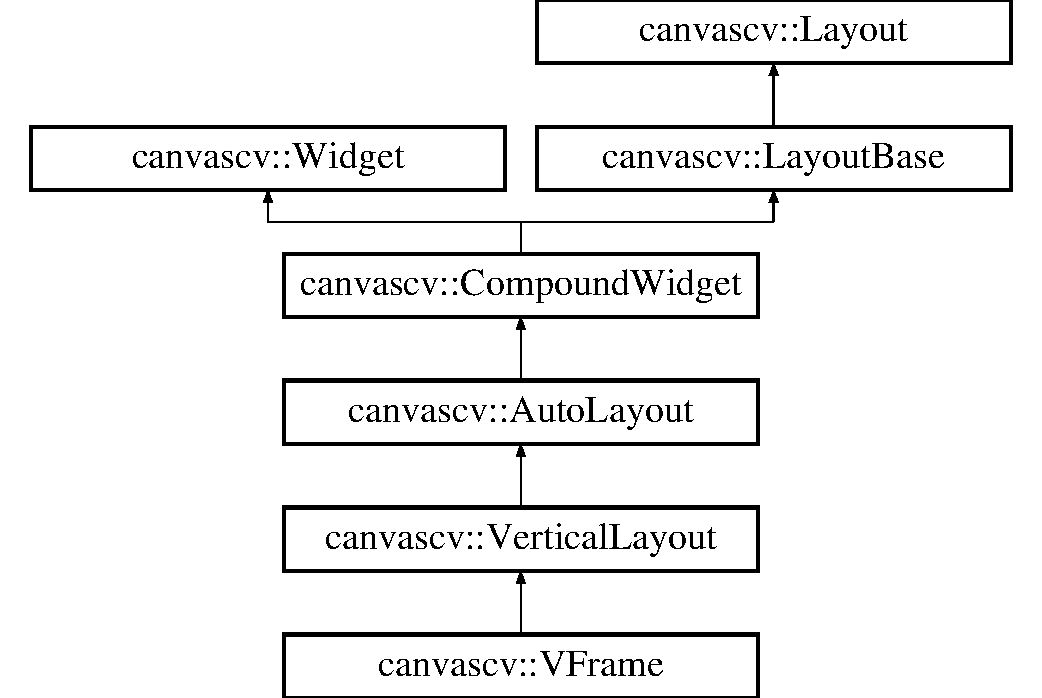
\includegraphics[height=6.000000cm]{classcanvascv_1_1VerticalLayout}
\end{center}
\end{figure}
\subsection*{Public Member Functions}
\begin{DoxyCompactItemize}
\item 
int \hyperlink{classcanvascv_1_1VerticalLayout_a49f7dd2e6eb7f60df3489069b4af500e}{get\+Spacing} () const \hypertarget{classcanvascv_1_1VerticalLayout_a49f7dd2e6eb7f60df3489069b4af500e}{}\label{classcanvascv_1_1VerticalLayout_a49f7dd2e6eb7f60df3489069b4af500e}

\begin{DoxyCompactList}\small\item\em returns pixel spacing between items \end{DoxyCompactList}\item 
void \hyperlink{classcanvascv_1_1VerticalLayout_ae3f58b90e8d957642feb2cc5e3100bd1}{set\+Spacing} (int value)\hypertarget{classcanvascv_1_1VerticalLayout_ae3f58b90e8d957642feb2cc5e3100bd1}{}\label{classcanvascv_1_1VerticalLayout_ae3f58b90e8d957642feb2cc5e3100bd1}

\begin{DoxyCompactList}\small\item\em sets pixel spacing between items \end{DoxyCompactList}\item 
virtual const char $\ast$ \hyperlink{classcanvascv_1_1VerticalLayout_a1b6eaaa782a4c9c880feb49d595d45b6}{get\+Type} () const 
\begin{DoxyCompactList}\small\item\em get\+Type is always implemented by derived to return the same static pointer per widget. \end{DoxyCompactList}\end{DoxyCompactItemize}
\subsection*{Static Public Member Functions}
\begin{DoxyCompactItemize}
\item 
static std\+::shared\+\_\+ptr$<$ \hyperlink{classcanvascv_1_1VerticalLayout}{Vertical\+Layout} $>$ \hyperlink{classcanvascv_1_1VerticalLayout_a3e0ae249db062663815d2d822e178dd3}{create} (\hyperlink{classcanvascv_1_1Layout}{Layout} \&layout, const cv\+::\+Point \&pos=cv\+::\+Point(0, 0))
\begin{DoxyCompactList}\small\item\em create a \hyperlink{classcanvascv_1_1VerticalLayout}{Vertical\+Layout} widget \end{DoxyCompactList}\end{DoxyCompactItemize}
\subsection*{Protected Member Functions}
\begin{DoxyCompactItemize}
\item 
virtual void \hyperlink{classcanvascv_1_1VerticalLayout_a0d4661776d5cb6dc4eccebcb3e5ff17c}{recalc\+Compound} ()
\begin{DoxyCompactList}\small\item\em recalc\+Compound \end{DoxyCompactList}\end{DoxyCompactItemize}
\subsection*{Additional Inherited Members}


\subsection{Detailed Description}
A \hyperlink{classcanvascv_1_1Layout}{Layout} implementation which lays it\textquotesingle{}s internal widgets vertically with a predefined spacing between widgets.
\begin{DoxyItemize}
\item Vertical layout is automatic according to widget size and spacing.
\begin{DoxyEnumerate}
\item This layout can expand up (it\textquotesingle{}s \textquotesingle{}flow\+Anchor\textquotesingle{} is B\+O\+T\+T\+OM), or down (it\textquotesingle{}s \textquotesingle{}flow\+Anchor\textquotesingle{} is T\+OP)
\end{DoxyEnumerate}
\item Horizontal layout per laid widget is determined according to the laid widget \textquotesingle{}layout\+Anchor\textquotesingle{}\+:
\begin{DoxyEnumerate}
\item L\+E\+FT will align the widget to the left (unless \hyperlink{classcanvascv_1_1Widget_a7cdddebd755c499712793f727a057733}{set\+Stretch\+X()} is true in the laid widget)
\item C\+E\+N\+T\+ER will align the widget to the center (unless \hyperlink{classcanvascv_1_1Widget_a7cdddebd755c499712793f727a057733}{set\+Stretch\+X()} is true in the laid widget)
\item R\+I\+G\+HT will align the widget to the right (unless \hyperlink{classcanvascv_1_1Widget_a7cdddebd755c499712793f727a057733}{set\+Stretch\+X()} is true in the laid widget) \begin{DoxyVerb}   +----------------------+
   |       PADDING        |
   | P +--------+       P |
   | A | Widget |       A |  layoutAnchor = LEFT
   | D +--------+       D |
   | D     SPACING      D |
   | I   +----------+   I |
   | N   |  Widget  |   N |  layoutAnchor = CENTER
   | G   +----------+   G |
   |       SPACING        |
   |        +---------+   |
   | P      | Widget  | P |  layoutAnchor = RIGHT
   | A      +---------+ A |
   | D     SPACING      D |
   | D +--------------+ D |
   | I |   Widget     | I |  layoutAnchor=whatever...(widest sets the standard for other)
   | N +--------------+ N |
   | G     PADDING      G |
   +----------------------+
\end{DoxyVerb}
 
\end{DoxyEnumerate}
\end{DoxyItemize}

\subsection{Member Function Documentation}
\index{canvascv\+::\+Vertical\+Layout@{canvascv\+::\+Vertical\+Layout}!create@{create}}
\index{create@{create}!canvascv\+::\+Vertical\+Layout@{canvascv\+::\+Vertical\+Layout}}
\subsubsection[{\texorpdfstring{create(\+Layout \&layout, const cv\+::\+Point \&pos=cv\+::\+Point(0, 0))}{create(Layout &layout, const cv::Point &pos=cv::Point(0, 0))}}]{\setlength{\rightskip}{0pt plus 5cm}static std\+::shared\+\_\+ptr$<${\bf Vertical\+Layout}$>$ canvascv\+::\+Vertical\+Layout\+::create (
\begin{DoxyParamCaption}
\item[{{\bf Layout} \&}]{layout, }
\item[{const cv\+::\+Point \&}]{pos = {\ttfamily cv\+:\+:Point(0,~0)}}
\end{DoxyParamCaption}
)\hspace{0.3cm}{\ttfamily [static]}}\hypertarget{classcanvascv_1_1VerticalLayout_a3e0ae249db062663815d2d822e178dd3}{}\label{classcanvascv_1_1VerticalLayout_a3e0ae249db062663815d2d822e178dd3}

\begin{DoxyParams}{Parameters}
{\em layout} & widgets are placed in layouts Canvas/\+V\+Frame/\+H\+Frame/... \\
\hline
{\em pos} & location in the \hyperlink{classcanvascv_1_1Layout}{Layout} (Layouts can ignore that) \\
\hline
\end{DoxyParams}
\begin{DoxyReturn}{Returns}
a smart pointer copy of the object kept in the \hyperlink{classcanvascv_1_1Layout}{Layout} 
\end{DoxyReturn}
\index{canvascv\+::\+Vertical\+Layout@{canvascv\+::\+Vertical\+Layout}!get\+Type@{get\+Type}}
\index{get\+Type@{get\+Type}!canvascv\+::\+Vertical\+Layout@{canvascv\+::\+Vertical\+Layout}}
\subsubsection[{\texorpdfstring{get\+Type() const }{getType() const }}]{\setlength{\rightskip}{0pt plus 5cm}virtual const char$\ast$ canvascv\+::\+Vertical\+Layout\+::get\+Type (
\begin{DoxyParamCaption}
{}
\end{DoxyParamCaption}
) const\hspace{0.3cm}{\ttfamily [virtual]}}\hypertarget{classcanvascv_1_1VerticalLayout_a1b6eaaa782a4c9c880feb49d595d45b6}{}\label{classcanvascv_1_1VerticalLayout_a1b6eaaa782a4c9c880feb49d595d45b6}
\begin{DoxyReturn}{Returns}
const char $\ast$ pointer to string with widget type name 
\end{DoxyReturn}


Implements \hyperlink{classcanvascv_1_1Widget_a85884269bd53ab91203f099a586efa43}{canvascv\+::\+Widget}.



Reimplemented in \hyperlink{classcanvascv_1_1VFrame_a8a87d2a05ca0f42a8deeaefa698347a9}{canvascv\+::\+V\+Frame}.

\index{canvascv\+::\+Vertical\+Layout@{canvascv\+::\+Vertical\+Layout}!recalc\+Compound@{recalc\+Compound}}
\index{recalc\+Compound@{recalc\+Compound}!canvascv\+::\+Vertical\+Layout@{canvascv\+::\+Vertical\+Layout}}
\subsubsection[{\texorpdfstring{recalc\+Compound()}{recalcCompound()}}]{\setlength{\rightskip}{0pt plus 5cm}virtual void canvascv\+::\+Vertical\+Layout\+::recalc\+Compound (
\begin{DoxyParamCaption}
{}
\end{DoxyParamCaption}
)\hspace{0.3cm}{\ttfamily [protected]}, {\ttfamily [virtual]}}\hypertarget{classcanvascv_1_1VerticalLayout_a0d4661776d5cb6dc4eccebcb3e5ff17c}{}\label{classcanvascv_1_1VerticalLayout_a0d4661776d5cb6dc4eccebcb3e5ff17c}
Your BG size recalculation/allocation and FG drawing is done here. It is done semi automatically. Is you invoke setters in this method on your internal widgets, then make sure to update them and/or their layout 

Implements \hyperlink{classcanvascv_1_1CompoundWidget_a4a4f8241d6fd187ffcae2c7968f13864}{canvascv\+::\+Compound\+Widget}.



The documentation for this class was generated from the following file\+:\begin{DoxyCompactItemize}
\item 
Canvas\+C\+V-\/doxygen/src/canvascv/widgets/verticallayout.\+h\end{DoxyCompactItemize}

\hypertarget{classcanvascv_1_1VFrame}{}\section{canvascv\+:\+:V\+Frame Class Reference}
\label{classcanvascv_1_1VFrame}\index{canvascv\+::\+V\+Frame@{canvascv\+::\+V\+Frame}}


The \hyperlink{classcanvascv_1_1VFrame}{V\+Frame} class.  




{\ttfamily \#include $<$vframe.\+h$>$}

Inheritance diagram for canvascv\+:\+:V\+Frame\+:\begin{figure}[H]
\begin{center}
\leavevmode
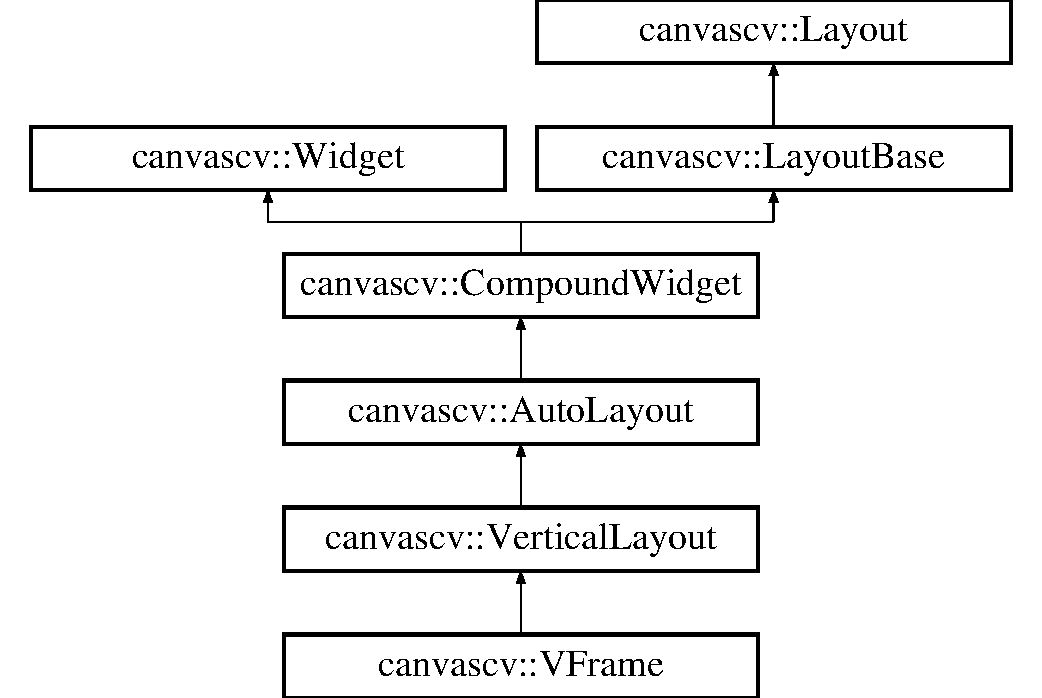
\includegraphics[height=6.000000cm]{classcanvascv_1_1VFrame}
\end{center}
\end{figure}
\subsection*{Public Member Functions}
\begin{DoxyCompactItemize}
\item 
void \hyperlink{classcanvascv_1_1VFrame_aa99d2a36a61eca36d3e3ba0972df65b4}{set\+Frame\+Relief} (\hyperlink{classcanvascv_1_1Widget_a8253daa509c55c24c92ce0d3dd93e4cd}{Relief} value)
\begin{DoxyCompactList}\small\item\em set\+Frame\+Relief \end{DoxyCompactList}\item 
virtual const char $\ast$ \hyperlink{classcanvascv_1_1VFrame_a8a87d2a05ca0f42a8deeaefa698347a9}{get\+Type} () const 
\begin{DoxyCompactList}\small\item\em get\+Type is always implemented by derived to return the same static pointer per widget. \end{DoxyCompactList}\end{DoxyCompactItemize}
\subsection*{Static Public Member Functions}
\begin{DoxyCompactItemize}
\item 
static std\+::shared\+\_\+ptr$<$ \hyperlink{classcanvascv_1_1VFrame}{V\+Frame} $>$ \hyperlink{classcanvascv_1_1VFrame_a013de150c59b8f7f37aa21ac59d78b10}{create} (\hyperlink{classcanvascv_1_1Layout}{Layout} \&layout, const cv\+::\+Point \&pos=cv\+::\+Point(0, 0))
\begin{DoxyCompactList}\small\item\em create a \hyperlink{classcanvascv_1_1VFrame}{V\+Frame} widget \end{DoxyCompactList}\end{DoxyCompactItemize}
\subsection*{Additional Inherited Members}


\subsection{Detailed Description}
A frame with a background of a selected relief type. This is also a \hyperlink{classcanvascv_1_1Layout}{Layout} for other Widgets and it lays them vertically. \begin{DoxySeeAlso}{See also}
\hyperlink{classcanvascv_1_1VerticalLayout}{Vertical\+Layout} 
\end{DoxySeeAlso}
\begin{Desc}
\item[Examples\+: ]\par
\hyperlink{example_add_widget_8cpp-example}{example\+\_\+add\+\_\+widget.\+cpp}.\end{Desc}


\subsection{Member Function Documentation}
\index{canvascv\+::\+V\+Frame@{canvascv\+::\+V\+Frame}!create@{create}}
\index{create@{create}!canvascv\+::\+V\+Frame@{canvascv\+::\+V\+Frame}}
\subsubsection[{\texorpdfstring{create(\+Layout \&layout, const cv\+::\+Point \&pos=cv\+::\+Point(0, 0))}{create(Layout &layout, const cv::Point &pos=cv::Point(0, 0))}}]{\setlength{\rightskip}{0pt plus 5cm}static std\+::shared\+\_\+ptr$<${\bf V\+Frame}$>$ canvascv\+::\+V\+Frame\+::create (
\begin{DoxyParamCaption}
\item[{{\bf Layout} \&}]{layout, }
\item[{const cv\+::\+Point \&}]{pos = {\ttfamily cv\+:\+:Point(0,~0)}}
\end{DoxyParamCaption}
)\hspace{0.3cm}{\ttfamily [static]}}\hypertarget{classcanvascv_1_1VFrame_a013de150c59b8f7f37aa21ac59d78b10}{}\label{classcanvascv_1_1VFrame_a013de150c59b8f7f37aa21ac59d78b10}

\begin{DoxyParams}{Parameters}
{\em layout} & widgets are placed in layouts Canvas/\+V\+Frame/\+H\+Frame/... \\
\hline
{\em pos} & location in the \hyperlink{classcanvascv_1_1Layout}{Layout} (Layouts can ignore that) \\
\hline
\end{DoxyParams}
\begin{DoxyReturn}{Returns}
a smart pointer copy of the object kept in the \hyperlink{classcanvascv_1_1Layout}{Layout} 
\end{DoxyReturn}
\begin{Desc}
\item[Examples\+: ]\par
\hyperlink{example_add_widget_8cpp-example}{example\+\_\+add\+\_\+widget.\+cpp}, and \hyperlink{example_shapes_widgets_8cpp-example}{example\+\_\+shapes\+\_\+widgets.\+cpp}.\end{Desc}
\index{canvascv\+::\+V\+Frame@{canvascv\+::\+V\+Frame}!get\+Type@{get\+Type}}
\index{get\+Type@{get\+Type}!canvascv\+::\+V\+Frame@{canvascv\+::\+V\+Frame}}
\subsubsection[{\texorpdfstring{get\+Type() const }{getType() const }}]{\setlength{\rightskip}{0pt plus 5cm}virtual const char$\ast$ canvascv\+::\+V\+Frame\+::get\+Type (
\begin{DoxyParamCaption}
{}
\end{DoxyParamCaption}
) const\hspace{0.3cm}{\ttfamily [virtual]}}\hypertarget{classcanvascv_1_1VFrame_a8a87d2a05ca0f42a8deeaefa698347a9}{}\label{classcanvascv_1_1VFrame_a8a87d2a05ca0f42a8deeaefa698347a9}
\begin{DoxyReturn}{Returns}
const char $\ast$ pointer to string with widget type name 
\end{DoxyReturn}


Reimplemented from \hyperlink{classcanvascv_1_1VerticalLayout_a1b6eaaa782a4c9c880feb49d595d45b6}{canvascv\+::\+Vertical\+Layout}.

\index{canvascv\+::\+V\+Frame@{canvascv\+::\+V\+Frame}!set\+Frame\+Relief@{set\+Frame\+Relief}}
\index{set\+Frame\+Relief@{set\+Frame\+Relief}!canvascv\+::\+V\+Frame@{canvascv\+::\+V\+Frame}}
\subsubsection[{\texorpdfstring{set\+Frame\+Relief(\+Relief value)}{setFrameRelief(Relief value)}}]{\setlength{\rightskip}{0pt plus 5cm}void canvascv\+::\+V\+Frame\+::set\+Frame\+Relief (
\begin{DoxyParamCaption}
\item[{{\bf Relief}}]{value}
\end{DoxyParamCaption}
)}\hypertarget{classcanvascv_1_1VFrame_aa99d2a36a61eca36d3e3ba0972df65b4}{}\label{classcanvascv_1_1VFrame_aa99d2a36a61eca36d3e3ba0972df65b4}

\begin{DoxyParams}{Parameters}
{\em value} & is one of the supported relief types \\
\hline
\end{DoxyParams}
\begin{DoxySeeAlso}{See also}
\hyperlink{classcanvascv_1_1Widget_a8253daa509c55c24c92ce0d3dd93e4cd}{Widget\+::\+Relief} 
\end{DoxySeeAlso}


The documentation for this class was generated from the following file\+:\begin{DoxyCompactItemize}
\item 
Canvas\+C\+V-\/doxygen/src/canvascv/widgets/vframe.\+h\end{DoxyCompactItemize}

\hypertarget{classcanvascv_1_1Widget}{}\section{canvascv\+:\+:Widget Class Reference}
\label{classcanvascv_1_1Widget}\index{canvascv\+::\+Widget@{canvascv\+::\+Widget}}


The \hyperlink{classcanvascv_1_1Widget}{Widget} class.  




{\ttfamily \#include $<$widget.\+h$>$}

Inheritance diagram for canvascv\+:\+:Widget\+:\begin{figure}[H]
\begin{center}
\leavevmode
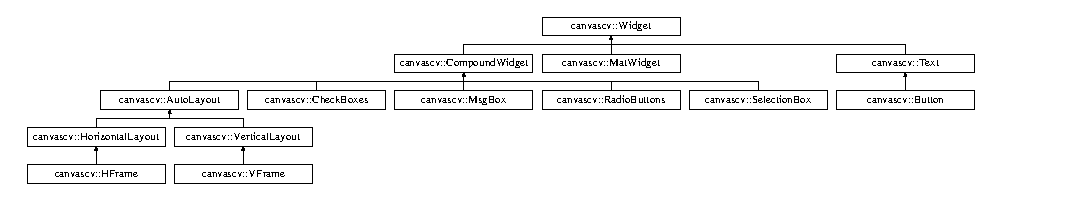
\includegraphics[height=2.234637cm]{classcanvascv_1_1Widget}
\end{center}
\end{figure}
\subsection*{Public Types}
\begin{DoxyCompactItemize}
\item 
typedef std\+::function$<$ void(\hyperlink{classcanvascv_1_1Widget}{Widget} $\ast$)$>$ \hyperlink{classcanvascv_1_1Widget_ad27bca771ee1c14454c77c91d9d49925}{C\+B\+Widget}\hypertarget{classcanvascv_1_1Widget_ad27bca771ee1c14454c77c91d9d49925}{}\label{classcanvascv_1_1Widget_ad27bca771ee1c14454c77c91d9d49925}

\begin{DoxyCompactList}\small\item\em signature of a callback which only gets the widget \end{DoxyCompactList}\item 
typedef std\+::function$<$ void(\hyperlink{classcanvascv_1_1Widget}{Widget} $\ast$, \hyperlink{classcanvascv_1_1Widget_afc39a6533455cbc3161ae3a021da0dc8}{State})$>$ \hyperlink{classcanvascv_1_1Widget_a410a6951e3d1f30b87702577a389d937}{C\+B\+Widget\+State}\hypertarget{classcanvascv_1_1Widget_a410a6951e3d1f30b87702577a389d937}{}\label{classcanvascv_1_1Widget_a410a6951e3d1f30b87702577a389d937}

\begin{DoxyCompactList}\small\item\em signature of a callback which gets the State \end{DoxyCompactList}\item 
typedef std\+::function$<$ void(\hyperlink{classcanvascv_1_1Widget}{Widget} $\ast$, int)$>$ \hyperlink{classcanvascv_1_1Widget_a977cbd39cf203c5866f07f3645c7e4bc}{C\+B\+User\+Selection}\hypertarget{classcanvascv_1_1Widget_a977cbd39cf203c5866f07f3645c7e4bc}{}\label{classcanvascv_1_1Widget_a977cbd39cf203c5866f07f3645c7e4bc}

\begin{DoxyCompactList}\small\item\em signature of a callback which gets a user selection \end{DoxyCompactList}\end{DoxyCompactItemize}
\subsection*{Public Member Functions}
\begin{DoxyCompactItemize}
\item 
\hyperlink{classcanvascv_1_1Widget_a1879deafb7cb8ad80e2262568ef2bde1}{Widget} (const cv\+::\+Point \&pos=cv\+::\+Point(0, 0))\hypertarget{classcanvascv_1_1Widget_a1879deafb7cb8ad80e2262568ef2bde1}{}\label{classcanvascv_1_1Widget_a1879deafb7cb8ad80e2262568ef2bde1}

\begin{DoxyCompactList}\small\item\em constructor \end{DoxyCompactList}\item 
virtual \hyperlink{classcanvascv_1_1Widget_abaa2a6266a947194fe240e9385cfaa6f}{$\sim$\+Widget} ()\hypertarget{classcanvascv_1_1Widget_abaa2a6266a947194fe240e9385cfaa6f}{}\label{classcanvascv_1_1Widget_abaa2a6266a947194fe240e9385cfaa6f}

\begin{DoxyCompactList}\small\item\em virtual destructor \end{DoxyCompactList}\item 
virtual const char $\ast$ \hyperlink{classcanvascv_1_1Widget_a85884269bd53ab91203f099a586efa43}{get\+Type} () const =0
\begin{DoxyCompactList}\small\item\em get\+Type is always implemented by derived to return the same static pointer per widget. \end{DoxyCompactList}\item 
void \hyperlink{classcanvascv_1_1Widget_abdb1aed0ca76845ba6a56c4f8db502c9}{notify\+On\+Change} (\hyperlink{classcanvascv_1_1Widget_a410a6951e3d1f30b87702577a389d937}{C\+B\+Widget\+State} cb)
\begin{DoxyCompactList}\small\item\em used to register for notifications on a widget \end{DoxyCompactList}\item 
cv\+::\+Scalar \hyperlink{classcanvascv_1_1Widget_aadbc81d960f158f2e3c8e0d96167408e}{get\+Outline\+Color} () const \hypertarget{classcanvascv_1_1Widget_aadbc81d960f158f2e3c8e0d96167408e}{}\label{classcanvascv_1_1Widget_aadbc81d960f158f2e3c8e0d96167408e}

\begin{DoxyCompactList}\small\item\em get the outline color \end{DoxyCompactList}\item 
virtual void \hyperlink{classcanvascv_1_1Widget_a6e79b6a861cfb54fea56d5705fec44d7}{set\+Outline\+Color} (const cv\+::\+Scalar \&value)\hypertarget{classcanvascv_1_1Widget_a6e79b6a861cfb54fea56d5705fec44d7}{}\label{classcanvascv_1_1Widget_a6e79b6a861cfb54fea56d5705fec44d7}

\begin{DoxyCompactList}\small\item\em set the outline color \end{DoxyCompactList}\item 
cv\+::\+Scalar \hyperlink{classcanvascv_1_1Widget_a0563e98b43c8eba6760a3f5157619104}{get\+Fill\+Color} () const \hypertarget{classcanvascv_1_1Widget_a0563e98b43c8eba6760a3f5157619104}{}\label{classcanvascv_1_1Widget_a0563e98b43c8eba6760a3f5157619104}

\begin{DoxyCompactList}\small\item\em get the bg color \end{DoxyCompactList}\item 
virtual void \hyperlink{classcanvascv_1_1Widget_a527b421eb4503da4275df8f6685ad8ea}{set\+Fill\+Color} (const cv\+::\+Scalar \&value)\hypertarget{classcanvascv_1_1Widget_a527b421eb4503da4275df8f6685ad8ea}{}\label{classcanvascv_1_1Widget_a527b421eb4503da4275df8f6685ad8ea}

\begin{DoxyCompactList}\small\item\em set the bg color \end{DoxyCompactList}\item 
bool \hyperlink{classcanvascv_1_1Widget_adc23c79ecc1cbb20343a678854b82c9f}{get\+Visible} () const \hypertarget{classcanvascv_1_1Widget_adc23c79ecc1cbb20343a678854b82c9f}{}\label{classcanvascv_1_1Widget_adc23c79ecc1cbb20343a678854b82c9f}

\begin{DoxyCompactList}\small\item\em is the widget visible \end{DoxyCompactList}\item 
virtual void \hyperlink{classcanvascv_1_1Widget_a3c9bd8b6b90dbe3958e452e04843feb1}{set\+Visible} (bool value)\hypertarget{classcanvascv_1_1Widget_a3c9bd8b6b90dbe3958e452e04843feb1}{}\label{classcanvascv_1_1Widget_a3c9bd8b6b90dbe3958e452e04843feb1}

\begin{DoxyCompactList}\small\item\em set the widget visible state \end{DoxyCompactList}\item 
int \hyperlink{classcanvascv_1_1Widget_a75c8818ca95f88f674d9e4668c5071c6}{get\+Thickness} () const \hypertarget{classcanvascv_1_1Widget_a75c8818ca95f88f674d9e4668c5071c6}{}\label{classcanvascv_1_1Widget_a75c8818ca95f88f674d9e4668c5071c6}

\begin{DoxyCompactList}\small\item\em get line thickness to use when drawing \end{DoxyCompactList}\item 
virtual void \hyperlink{classcanvascv_1_1Widget_a8514776cac6c75fb723eefafa9b5b8b6}{set\+Thickness} (int value)\hypertarget{classcanvascv_1_1Widget_a8514776cac6c75fb723eefafa9b5b8b6}{}\label{classcanvascv_1_1Widget_a8514776cac6c75fb723eefafa9b5b8b6}

\begin{DoxyCompactList}\small\item\em set line thickness to use when drawing \end{DoxyCompactList}\item 
int \hyperlink{classcanvascv_1_1Widget_a09656f51cc84ab95048191083ff7cfa7}{get\+Line\+Type} () const \hypertarget{classcanvascv_1_1Widget_a09656f51cc84ab95048191083ff7cfa7}{}\label{classcanvascv_1_1Widget_a09656f51cc84ab95048191083ff7cfa7}

\begin{DoxyCompactList}\small\item\em get the line type (L\+I\+N\+E\+\_\+4, L\+I\+N\+E\+\_\+8, L\+I\+N\+E\+\_\+\+AA) \end{DoxyCompactList}\item 
virtual void \hyperlink{classcanvascv_1_1Widget_ad61f8a9fe81e1d1e7247a83b2eefc52a}{set\+Line\+Type} (int value)\hypertarget{classcanvascv_1_1Widget_ad61f8a9fe81e1d1e7247a83b2eefc52a}{}\label{classcanvascv_1_1Widget_ad61f8a9fe81e1d1e7247a83b2eefc52a}

\begin{DoxyCompactList}\small\item\em set the line type (L\+I\+N\+E\+\_\+4, L\+I\+N\+E\+\_\+8, L\+I\+N\+E\+\_\+\+AA) \end{DoxyCompactList}\item 
uchar \hyperlink{classcanvascv_1_1Widget_a5e7e4bfb43a2c8179114ed63a2e25cff}{get\+Alpha} () const \hypertarget{classcanvascv_1_1Widget_a5e7e4bfb43a2c8179114ed63a2e25cff}{}\label{classcanvascv_1_1Widget_a5e7e4bfb43a2c8179114ed63a2e25cff}

\begin{DoxyCompactList}\small\item\em get the alpha value used for the widge background \mbox{[}0,255\mbox{]} =$>$ \mbox{[}transparent,opaque\mbox{]} \end{DoxyCompactList}\item 
void \hyperlink{classcanvascv_1_1Widget_a4c16525b31e70acd43372af0c1e60d42}{set\+Alpha} (uchar value)\hypertarget{classcanvascv_1_1Widget_a4c16525b31e70acd43372af0c1e60d42}{}\label{classcanvascv_1_1Widget_a4c16525b31e70acd43372af0c1e60d42}

\begin{DoxyCompactList}\small\item\em set the alpha value used for the widge background \mbox{[}0,255\mbox{]} =$>$ \mbox{[}transparent,opaque\mbox{]} \end{DoxyCompactList}\item 
\hyperlink{classcanvascv_1_1Widget_a98ca3c300ba50b316fa5a1d300456abe}{Anchor} \hyperlink{classcanvascv_1_1Widget_a3b460d40be2a634153bf0785c46383b9}{get\+Layout\+Anchor} () const 
\begin{DoxyCompactList}\small\item\em get\+Layout\+Anchor returns the anchor for using in the \hyperlink{classcanvascv_1_1Layout}{Layout} we\textquotesingle{}re in \end{DoxyCompactList}\item 
void \hyperlink{classcanvascv_1_1Widget_a7180ca0054874c853e805e7842741596}{set\+Layout\+Anchor} (const \hyperlink{classcanvascv_1_1Widget_a98ca3c300ba50b316fa5a1d300456abe}{Anchor} \&value)
\begin{DoxyCompactList}\small\item\em set\+Layout\+Anchor sets the anchor for using in the \hyperlink{classcanvascv_1_1Layout}{Layout} we\textquotesingle{}re in \end{DoxyCompactList}\item 
\hyperlink{classcanvascv_1_1Widget_a98ca3c300ba50b316fa5a1d300456abe}{Anchor} \hyperlink{classcanvascv_1_1Widget_a4956e8b0ced615c3177dc38f553732fb}{get\+Flow\+Anchor} () const 
\begin{DoxyCompactList}\small\item\em get\+Flow\+Anchor get internal widget alignment and direction of growth \end{DoxyCompactList}\item 
void \hyperlink{classcanvascv_1_1Widget_a69f455f7fbf67f636ee1155795057b87}{set\+Flow\+Anchor} (const \hyperlink{classcanvascv_1_1Widget_a98ca3c300ba50b316fa5a1d300456abe}{Anchor} \&value)
\begin{DoxyCompactList}\small\item\em set\+Flow\+Anchor set internal widget alignment and direction of growth \end{DoxyCompactList}\item 
int \hyperlink{classcanvascv_1_1Widget_af68aa024314497681d3f1cac1c511d53}{get\+Id} ()\hypertarget{classcanvascv_1_1Widget_af68aa024314497681d3f1cac1c511d53}{}\label{classcanvascv_1_1Widget_af68aa024314497681d3f1cac1c511d53}

\begin{DoxyCompactList}\small\item\em Widgets have a unique id per instance. \end{DoxyCompactList}\item 
virtual const std\+::string \& \hyperlink{classcanvascv_1_1Widget_a5619c96f65d3853f2463043a814191ac}{get\+Status\+Msg} () const 
\begin{DoxyCompactList}\small\item\em get\+Status\+Msg \end{DoxyCompactList}\item 
void \hyperlink{classcanvascv_1_1Widget_ac882ef922394c8d55cc824bf83be0004}{set\+Status\+Msg} (const std\+::string \&value)
\begin{DoxyCompactList}\small\item\em set\+Status\+Msg \end{DoxyCompactList}\item 
const cv\+::\+Point \& \hyperlink{classcanvascv_1_1Widget_a22aa393604eaa7fe6645a0b6422db9e6}{get\+Location} () const \hypertarget{classcanvascv_1_1Widget_a22aa393604eaa7fe6645a0b6422db9e6}{}\label{classcanvascv_1_1Widget_a22aa393604eaa7fe6645a0b6422db9e6}

\begin{DoxyCompactList}\small\item\em get widget position in \hyperlink{classcanvascv_1_1Canvas}{Canvas} \end{DoxyCompactList}\item 
virtual void \hyperlink{classcanvascv_1_1Widget_a8a36b15a1c777baffbb4fcd4ccda3c45}{set\+Location} (const cv\+::\+Point \&value)\hypertarget{classcanvascv_1_1Widget_a8a36b15a1c777baffbb4fcd4ccda3c45}{}\label{classcanvascv_1_1Widget_a8a36b15a1c777baffbb4fcd4ccda3c45}

\begin{DoxyCompactList}\small\item\em set widget position in \hyperlink{classcanvascv_1_1Canvas}{Canvas} \end{DoxyCompactList}\item 
virtual void \hyperlink{classcanvascv_1_1Widget_a05344fc28d0e558fd2e940e672329dec}{translate} (const cv\+::\+Point \&translation)\hypertarget{classcanvascv_1_1Widget_a05344fc28d0e558fd2e940e672329dec}{}\label{classcanvascv_1_1Widget_a05344fc28d0e558fd2e940e672329dec}

\begin{DoxyCompactList}\small\item\em move the widget \end{DoxyCompactList}\item 
bool \hyperlink{classcanvascv_1_1Widget_a7cc134719de14cfb5b391e1a950a4840}{get\+StretchX} () const \hypertarget{classcanvascv_1_1Widget_a7cc134719de14cfb5b391e1a950a4840}{}\label{classcanvascv_1_1Widget_a7cc134719de14cfb5b391e1a950a4840}

\begin{DoxyCompactList}\small\item\em get if the \hyperlink{classcanvascv_1_1Layout}{Layout} we\textquotesingle{}re in should stretch us in the X direction \end{DoxyCompactList}\item 
void \hyperlink{classcanvascv_1_1Widget_a7cdddebd755c499712793f727a057733}{set\+StretchX} (bool value)\hypertarget{classcanvascv_1_1Widget_a7cdddebd755c499712793f727a057733}{}\label{classcanvascv_1_1Widget_a7cdddebd755c499712793f727a057733}

\begin{DoxyCompactList}\small\item\em set if the \hyperlink{classcanvascv_1_1Layout}{Layout} we\textquotesingle{}re in should stretch us in the X direction (and calls set\+Stretch\+X\+To\+Parent(false)) \end{DoxyCompactList}\item 
bool \hyperlink{classcanvascv_1_1Widget_a267ab2d3df58dce8c1e823050d811157}{get\+StretchY} () const \hypertarget{classcanvascv_1_1Widget_a267ab2d3df58dce8c1e823050d811157}{}\label{classcanvascv_1_1Widget_a267ab2d3df58dce8c1e823050d811157}

\begin{DoxyCompactList}\small\item\em get if the \hyperlink{classcanvascv_1_1Layout}{Layout} we\textquotesingle{}re in should stretch us in the Y direction \end{DoxyCompactList}\item 
void \hyperlink{classcanvascv_1_1Widget_a3ef50b76d33c332cea4e632346b6df33}{set\+StretchY} (bool value)\hypertarget{classcanvascv_1_1Widget_a3ef50b76d33c332cea4e632346b6df33}{}\label{classcanvascv_1_1Widget_a3ef50b76d33c332cea4e632346b6df33}

\begin{DoxyCompactList}\small\item\em set if the \hyperlink{classcanvascv_1_1Layout}{Layout} we\textquotesingle{}re in should stretch us in the Y direction (and calls set\+Stretch\+Y\+To\+Parent(false)) \end{DoxyCompactList}\item 
cv\+::\+Scalar \hyperlink{classcanvascv_1_1Widget_a37432df7d7e0029c98154d99d1e621bc}{get\+Select\+Color} () const \hypertarget{classcanvascv_1_1Widget_a37432df7d7e0029c98154d99d1e621bc}{}\label{classcanvascv_1_1Widget_a37432df7d7e0029c98154d99d1e621bc}

\begin{DoxyCompactList}\small\item\em get the color to use when a widget is selected \end{DoxyCompactList}\item 
virtual void \hyperlink{classcanvascv_1_1Widget_a64e1123175981fca5219519fac987596}{set\+Select\+Color} (const cv\+::\+Scalar \&value)\hypertarget{classcanvascv_1_1Widget_a64e1123175981fca5219519fac987596}{}\label{classcanvascv_1_1Widget_a64e1123175981fca5219519fac987596}

\begin{DoxyCompactList}\small\item\em set the color to use when a widget is selected \end{DoxyCompactList}\item 
std\+::shared\+\_\+ptr$<$ \hyperlink{classcanvascv_1_1Widget}{Widget} $>$ \hyperlink{classcanvascv_1_1Widget_ac3f34f3b8b3b57f000e5f5182d6396ab}{rmv\+From\+Layout} ()\hypertarget{classcanvascv_1_1Widget_ac3f34f3b8b3b57f000e5f5182d6396ab}{}\label{classcanvascv_1_1Widget_ac3f34f3b8b3b57f000e5f5182d6396ab}

\begin{DoxyCompactList}\small\item\em get rid of the widget \end{DoxyCompactList}\item 
bool \hyperlink{classcanvascv_1_1Widget_a7a2e233c96587b142c6c937cc3bdeaa4}{get\+Is\+Selectable} () const \hypertarget{classcanvascv_1_1Widget_a7a2e233c96587b142c6c937cc3bdeaa4}{}\label{classcanvascv_1_1Widget_a7a2e233c96587b142c6c937cc3bdeaa4}

\begin{DoxyCompactList}\small\item\em get if the widget should appear as selected when the mouse is over it \end{DoxyCompactList}\item 
void \hyperlink{classcanvascv_1_1Widget_a2d873d23e3f7f07d2ea1a487ea4665e9}{set\+Is\+Selectable} (bool value)\hypertarget{classcanvascv_1_1Widget_a2d873d23e3f7f07d2ea1a487ea4665e9}{}\label{classcanvascv_1_1Widget_a2d873d23e3f7f07d2ea1a487ea4665e9}

\begin{DoxyCompactList}\small\item\em set if the widget should appear as selected when the mouse is over it \end{DoxyCompactList}\item 
int \hyperlink{classcanvascv_1_1Widget_a97720a3b8073edecd43fe32ad1ce4f93}{get\+Forced\+Width} () const \hypertarget{classcanvascv_1_1Widget_a97720a3b8073edecd43fe32ad1ce4f93}{}\label{classcanvascv_1_1Widget_a97720a3b8073edecd43fe32ad1ce4f93}

\begin{DoxyCompactList}\small\item\em get the forced width for this widget \end{DoxyCompactList}\item 
void \hyperlink{classcanvascv_1_1Widget_a2dec191f9e2be6a1a291e6da275adca5}{set\+Forced\+Width} (int value)\hypertarget{classcanvascv_1_1Widget_a2dec191f9e2be6a1a291e6da275adca5}{}\label{classcanvascv_1_1Widget_a2dec191f9e2be6a1a291e6da275adca5}

\begin{DoxyCompactList}\small\item\em set the forced width for this widget (and calls set\+Stretch\+X/set\+Stretch\+X\+To\+Parent(false)) \end{DoxyCompactList}\item 
int \hyperlink{classcanvascv_1_1Widget_afd30c281d961fa92498f1eea83c22e6a}{get\+Forced\+Height} () const \hypertarget{classcanvascv_1_1Widget_afd30c281d961fa92498f1eea83c22e6a}{}\label{classcanvascv_1_1Widget_afd30c281d961fa92498f1eea83c22e6a}

\begin{DoxyCompactList}\small\item\em get the forced height for this widget \end{DoxyCompactList}\item 
void \hyperlink{classcanvascv_1_1Widget_aa88e20a2d34e335b134213cccfdef529}{set\+Forced\+Height} (int value)\hypertarget{classcanvascv_1_1Widget_aa88e20a2d34e335b134213cccfdef529}{}\label{classcanvascv_1_1Widget_aa88e20a2d34e335b134213cccfdef529}

\begin{DoxyCompactList}\small\item\em set the forced height for this widget (and calls set\+Stretch\+Y/set\+Stretch\+Y\+To\+Parent(false)) \end{DoxyCompactList}\item 
void \hyperlink{classcanvascv_1_1Widget_a5cfbbfb73055a55d679c7519926793bc}{update} ()\hypertarget{classcanvascv_1_1Widget_a5cfbbfb73055a55d679c7519926793bc}{}\label{classcanvascv_1_1Widget_a5cfbbfb73055a55d679c7519926793bc}

\begin{DoxyCompactList}\small\item\em removes \textquotesingle{}dirty\textquotesingle{} state and invokes the derived \textquotesingle{}recalc/recalc\+Compound\textquotesingle{} \end{DoxyCompactList}\item 
bool \hyperlink{classcanvascv_1_1Widget_ae7ba2e02a399317607a2a5dcd3b4a800}{is\+Removed} () const \hypertarget{classcanvascv_1_1Widget_ae7ba2e02a399317607a2a5dcd3b4a800}{}\label{classcanvascv_1_1Widget_ae7ba2e02a399317607a2a5dcd3b4a800}

\begin{DoxyCompactList}\small\item\em returns true if the widget has no layout and false if it does \end{DoxyCompactList}\item 
virtual const cv\+::\+Rect \& \hyperlink{classcanvascv_1_1Widget_afa0105481f639d660de98287a879810c}{get\+Rect} ()=0\hypertarget{classcanvascv_1_1Widget_afa0105481f639d660de98287a879810c}{}\label{classcanvascv_1_1Widget_afa0105481f639d660de98287a879810c}

\begin{DoxyCompactList}\small\item\em Actual size the widget is occupying due to \hyperlink{classcanvascv_1_1Layout}{Layout} manager. \end{DoxyCompactList}\item 
bool \hyperlink{classcanvascv_1_1Widget_ac9c864272c04f65f233c470dec917930}{get\+Stretch\+X\+To\+Parent} () const \hypertarget{classcanvascv_1_1Widget_ac9c864272c04f65f233c470dec917930}{}\label{classcanvascv_1_1Widget_ac9c864272c04f65f233c470dec917930}

\begin{DoxyCompactList}\small\item\em get if this widget streches to parent layout width \end{DoxyCompactList}\item 
void \hyperlink{classcanvascv_1_1Widget_a7b1ed6190950de22565c244f5aac49a4}{set\+Stretch\+X\+To\+Parent} (bool value)\hypertarget{classcanvascv_1_1Widget_a7b1ed6190950de22565c244f5aac49a4}{}\label{classcanvascv_1_1Widget_a7b1ed6190950de22565c244f5aac49a4}

\begin{DoxyCompactList}\small\item\em set if this widget streches to parent layout width (and calls set\+Stretch\+X(false)) \end{DoxyCompactList}\item 
bool \hyperlink{classcanvascv_1_1Widget_a3423f2e0dab494c6da99d43d186760bc}{get\+Stretch\+Y\+To\+Parent} () const \hypertarget{classcanvascv_1_1Widget_a3423f2e0dab494c6da99d43d186760bc}{}\label{classcanvascv_1_1Widget_a3423f2e0dab494c6da99d43d186760bc}

\begin{DoxyCompactList}\small\item\em get if this widget streches to parent layout height \end{DoxyCompactList}\item 
void \hyperlink{classcanvascv_1_1Widget_a825028e2405bfdf9d92d372e60585703}{set\+Stretch\+Y\+To\+Parent} (bool value)\hypertarget{classcanvascv_1_1Widget_a825028e2405bfdf9d92d372e60585703}{}\label{classcanvascv_1_1Widget_a825028e2405bfdf9d92d372e60585703}

\begin{DoxyCompactList}\small\item\em set if this widget streches to parent layout height (and calls set\+Stretch\+Y(false)) \end{DoxyCompactList}\end{DoxyCompactItemize}
\subsection*{Protected Member Functions}
\begin{DoxyCompactItemize}
\item 
void \hyperlink{classcanvascv_1_1Widget_a5b94411875ff9f65b4da857e3ee2734a}{set\+State\+Changes\+BG} ()\hypertarget{classcanvascv_1_1Widget_a5b94411875ff9f65b4da857e3ee2734a}{}\label{classcanvascv_1_1Widget_a5b94411875ff9f65b4da857e3ee2734a}

\begin{DoxyCompactList}\small\item\em widgets like buttons change bg on mouse events \end{DoxyCompactList}\item 
void \hyperlink{classcanvascv_1_1Widget_a0102a02ca60dad4dafc4bb1d0bba046b}{allocate\+BG} (const cv\+::\+Size \&size)\hypertarget{classcanvascv_1_1Widget_a0102a02ca60dad4dafc4bb1d0bba046b}{}\label{classcanvascv_1_1Widget_a0102a02ca60dad4dafc4bb1d0bba046b}

\begin{DoxyCompactList}\small\item\em invokes \hyperlink{classcanvascv_1_1Theme_a5f8c0e382d893419f9097bbc07e04130}{Theme\+::allocate\+B\+G()} \end{DoxyCompactList}\item 
virtual void \hyperlink{classcanvascv_1_1Widget_a1d6d9b43efb60d591280cf5997380731}{recalc} ()=0\hypertarget{classcanvascv_1_1Widget_a1d6d9b43efb60d591280cf5997380731}{}\label{classcanvascv_1_1Widget_a1d6d9b43efb60d591280cf5997380731}

\begin{DoxyCompactList}\small\item\em update self so next call to \textquotesingle{}draw\textquotesingle{} will display correctly \end{DoxyCompactList}\item 
void \hyperlink{classcanvascv_1_1Widget_ae84a6b77b417f8b9eb6d2e4f8e0fde60}{flat\+Widget} ()\hypertarget{classcanvascv_1_1Widget_ae84a6b77b417f8b9eb6d2e4f8e0fde60}{}\label{classcanvascv_1_1Widget_ae84a6b77b417f8b9eb6d2e4f8e0fde60}

\begin{DoxyCompactList}\small\item\em delegate to \hyperlink{classcanvascv_1_1Theme}{Theme} \end{DoxyCompactList}\item 
void \hyperlink{classcanvascv_1_1Widget_a09cf72b5592a91ef0ff91a59c7d1852d}{raised\+Widget} ()\hypertarget{classcanvascv_1_1Widget_a09cf72b5592a91ef0ff91a59c7d1852d}{}\label{classcanvascv_1_1Widget_a09cf72b5592a91ef0ff91a59c7d1852d}

\begin{DoxyCompactList}\small\item\em delegate to \hyperlink{classcanvascv_1_1Theme}{Theme} \end{DoxyCompactList}\item 
void \hyperlink{classcanvascv_1_1Widget_ad4e11c2d30dc54520b80a442a07fb7a0}{sunken\+Widget} ()\hypertarget{classcanvascv_1_1Widget_ad4e11c2d30dc54520b80a442a07fb7a0}{}\label{classcanvascv_1_1Widget_ad4e11c2d30dc54520b80a442a07fb7a0}

\begin{DoxyCompactList}\small\item\em delegate to \hyperlink{classcanvascv_1_1Theme}{Theme} \end{DoxyCompactList}\item 
void \hyperlink{classcanvascv_1_1Widget_a92e0bbdd196ff9282ee738ad6861d4cb}{selected\+Widget} ()\hypertarget{classcanvascv_1_1Widget_a92e0bbdd196ff9282ee738ad6861d4cb}{}\label{classcanvascv_1_1Widget_a92e0bbdd196ff9282ee738ad6861d4cb}

\begin{DoxyCompactList}\small\item\em delegate to \hyperlink{classcanvascv_1_1Theme}{Theme} \end{DoxyCompactList}\item 
virtual void \hyperlink{classcanvascv_1_1Widget_a74130cdbcc974dfa7e8ceb9a53c112b9}{render\+On} (cv\+::\+Mat \&dst)
\begin{DoxyCompactList}\small\item\em render the widget to dst \end{DoxyCompactList}\item 
virtual void \hyperlink{classcanvascv_1_1Widget_a8143c9c92abd2a0e0e8ce4c3c50a0f7a}{draw\+FG} (cv\+::\+Mat \&dst)=0\hypertarget{classcanvascv_1_1Widget_a8143c9c92abd2a0e0e8ce4c3c50a0f7a}{}\label{classcanvascv_1_1Widget_a8143c9c92abd2a0e0e8ce4c3c50a0f7a}

\begin{DoxyCompactList}\small\item\em dst is the roi of the widget size and not the full image \end{DoxyCompactList}\item 
void \hyperlink{classcanvascv_1_1Widget_a4e25259aef4fd707add107f4e4229a9f}{call\+Draw\+FG} (bool pre\+Allocate\+Mat=true)\hypertarget{classcanvascv_1_1Widget_a4e25259aef4fd707add107f4e4229a9f}{}\label{classcanvascv_1_1Widget_a4e25259aef4fd707add107f4e4229a9f}

\begin{DoxyCompactList}\small\item\em helper method which delgates to draw\+FG for derived \end{DoxyCompactList}\item 
virtual const cv\+::\+Rect \& \hyperlink{classcanvascv_1_1Widget_a5bae1daca295a6d7e2d1932d76529207}{get\+Minimal\+Rect} ()=0\hypertarget{classcanvascv_1_1Widget_a5bae1daca295a6d7e2d1932d76529207}{}\label{classcanvascv_1_1Widget_a5bae1daca295a6d7e2d1932d76529207}

\begin{DoxyCompactList}\small\item\em Minimal size the widget coould have occupy. \end{DoxyCompactList}\item 
bool \hyperlink{classcanvascv_1_1Widget_ac98faa983ed13b0394ec1542d89997eb}{set\+Dirty} ()
\begin{DoxyCompactList}\small\item\em set\+Dirty \end{DoxyCompactList}\item 
virtual bool \hyperlink{classcanvascv_1_1Widget_a3ea1ca9e064178a5647ce04bc531655f}{is\+At\+Pos} (const cv\+::\+Point \&pos)
\begin{DoxyCompactList}\small\item\em is\+At\+Pos \end{DoxyCompactList}\end{DoxyCompactItemize}


\subsection{Detailed Description}
\begin{DoxyNote}{Note}
All widgets have a static create methods, which is the only way to create them. The create will return a shared\+\_\+ptr$<$\+T$>$ instance, which you don\textquotesingle{}t have to keep since another one is kept by the \hyperlink{classcanvascv_1_1Layout}{Layout} in which the widget is placed. Never use delete on a \hyperlink{classcanvascv_1_1Widget}{Widget} pointer. 
\end{DoxyNote}
\begin{Desc}
\item[Examples\+: ]\par
\hyperlink{example_add_theme_8cpp-example}{example\+\_\+add\+\_\+theme.\+cpp}, \hyperlink{example_add_widget_8cpp-example}{example\+\_\+add\+\_\+widget.\+cpp}, \hyperlink{example_checkboxes_8cpp-example}{example\+\_\+checkboxes.\+cpp}, \hyperlink{example_msgbox_8cpp-example}{example\+\_\+msgbox.\+cpp}, \hyperlink{example_radiobuttons_8cpp-example}{example\+\_\+radiobuttons.\+cpp}, \hyperlink{example_selectbox_8cpp-example}{example\+\_\+selectbox.\+cpp}, and \hyperlink{example_shapes_widgets_8cpp-example}{example\+\_\+shapes\+\_\+widgets.\+cpp}.\end{Desc}


\subsection{Member Enumeration Documentation}
\index{canvascv\+::\+Widget@{canvascv\+::\+Widget}!Anchor@{Anchor}}
\index{Anchor@{Anchor}!canvascv\+::\+Widget@{canvascv\+::\+Widget}}
\subsubsection[{\texorpdfstring{Anchor}{Anchor}}]{\setlength{\rightskip}{0pt plus 5cm}enum {\bf canvascv\+::\+Widget\+::\+Anchor}}\hypertarget{classcanvascv_1_1Widget_a98ca3c300ba50b316fa5a1d300456abe}{}\label{classcanvascv_1_1Widget_a98ca3c300ba50b316fa5a1d300456abe}
Used for both aligment in the \hyperlink{classcanvascv_1_1Layout}{Layout} we belong to and internal widget alignments \begin{DoxySeeAlso}{See also}
\hyperlink{classcanvascv_1_1Widget_a3b460d40be2a634153bf0785c46383b9}{get\+Layout\+Anchor()}, \hyperlink{classcanvascv_1_1Widget_a7180ca0054874c853e805e7842741596}{set\+Layout\+Anchor()}, \hyperlink{classcanvascv_1_1Widget_a4956e8b0ced615c3177dc38f553732fb}{get\+Flow\+Anchor()}, \hyperlink{classcanvascv_1_1Widget_a69f455f7fbf67f636ee1155795057b87}{set\+Flow\+Anchor()} 
\end{DoxySeeAlso}
\begin{Desc}
\item[Enumerator]\par
\begin{description}
\index{T\+OP@{T\+OP}!canvascv\+::\+Widget@{canvascv\+::\+Widget}}\index{canvascv\+::\+Widget@{canvascv\+::\+Widget}!T\+OP@{T\+OP}}\item[{\em 
T\+OP\hypertarget{classcanvascv_1_1Widget_a98ca3c300ba50b316fa5a1d300456abeaa6a2c9d829ceed729afe8cb2f51b2f0c}{}\label{classcanvascv_1_1Widget_a98ca3c300ba50b316fa5a1d300456abeaa6a2c9d829ceed729afe8cb2f51b2f0c}
}]top \index{B\+O\+T\+T\+OM@{B\+O\+T\+T\+OM}!canvascv\+::\+Widget@{canvascv\+::\+Widget}}\index{canvascv\+::\+Widget@{canvascv\+::\+Widget}!B\+O\+T\+T\+OM@{B\+O\+T\+T\+OM}}\item[{\em 
B\+O\+T\+T\+OM\hypertarget{classcanvascv_1_1Widget_a98ca3c300ba50b316fa5a1d300456abea8612ea17f4627ffaf6aa00af2595efe7}{}\label{classcanvascv_1_1Widget_a98ca3c300ba50b316fa5a1d300456abea8612ea17f4627ffaf6aa00af2595efe7}
}]bottom \index{L\+E\+FT@{L\+E\+FT}!canvascv\+::\+Widget@{canvascv\+::\+Widget}}\index{canvascv\+::\+Widget@{canvascv\+::\+Widget}!L\+E\+FT@{L\+E\+FT}}\item[{\em 
L\+E\+FT\hypertarget{classcanvascv_1_1Widget_a98ca3c300ba50b316fa5a1d300456abea684450835b6203aa50c0290911305c55}{}\label{classcanvascv_1_1Widget_a98ca3c300ba50b316fa5a1d300456abea684450835b6203aa50c0290911305c55}
}]left \index{R\+I\+G\+HT@{R\+I\+G\+HT}!canvascv\+::\+Widget@{canvascv\+::\+Widget}}\index{canvascv\+::\+Widget@{canvascv\+::\+Widget}!R\+I\+G\+HT@{R\+I\+G\+HT}}\item[{\em 
R\+I\+G\+HT\hypertarget{classcanvascv_1_1Widget_a98ca3c300ba50b316fa5a1d300456abeaa426f2ee5f621cfc973e1032931932ef}{}\label{classcanvascv_1_1Widget_a98ca3c300ba50b316fa5a1d300456abeaa426f2ee5f621cfc973e1032931932ef}
}]right \index{C\+E\+N\+T\+ER@{C\+E\+N\+T\+ER}!canvascv\+::\+Widget@{canvascv\+::\+Widget}}\index{canvascv\+::\+Widget@{canvascv\+::\+Widget}!C\+E\+N\+T\+ER@{C\+E\+N\+T\+ER}}\item[{\em 
C\+E\+N\+T\+ER\hypertarget{classcanvascv_1_1Widget_a98ca3c300ba50b316fa5a1d300456abea2cd62693af40f3c5f559a07d6a61a55d}{}\label{classcanvascv_1_1Widget_a98ca3c300ba50b316fa5a1d300456abea2cd62693af40f3c5f559a07d6a61a55d}
}]center \index{T\+O\+P\+\_\+\+L\+E\+FT@{T\+O\+P\+\_\+\+L\+E\+FT}!canvascv\+::\+Widget@{canvascv\+::\+Widget}}\index{canvascv\+::\+Widget@{canvascv\+::\+Widget}!T\+O\+P\+\_\+\+L\+E\+FT@{T\+O\+P\+\_\+\+L\+E\+FT}}\item[{\em 
T\+O\+P\+\_\+\+L\+E\+FT\hypertarget{classcanvascv_1_1Widget_a98ca3c300ba50b316fa5a1d300456abeade1c5e9202b56dcd7d2f5f9825a36cf9}{}\label{classcanvascv_1_1Widget_a98ca3c300ba50b316fa5a1d300456abeade1c5e9202b56dcd7d2f5f9825a36cf9}
}]top-\/left \index{T\+O\+P\+\_\+\+R\+I\+G\+HT@{T\+O\+P\+\_\+\+R\+I\+G\+HT}!canvascv\+::\+Widget@{canvascv\+::\+Widget}}\index{canvascv\+::\+Widget@{canvascv\+::\+Widget}!T\+O\+P\+\_\+\+R\+I\+G\+HT@{T\+O\+P\+\_\+\+R\+I\+G\+HT}}\item[{\em 
T\+O\+P\+\_\+\+R\+I\+G\+HT\hypertarget{classcanvascv_1_1Widget_a98ca3c300ba50b316fa5a1d300456abea28a2d9d47839ff200bcc800acc32bc92}{}\label{classcanvascv_1_1Widget_a98ca3c300ba50b316fa5a1d300456abea28a2d9d47839ff200bcc800acc32bc92}
}]top-\/right \index{B\+O\+T\+T\+O\+M\+\_\+\+L\+E\+FT@{B\+O\+T\+T\+O\+M\+\_\+\+L\+E\+FT}!canvascv\+::\+Widget@{canvascv\+::\+Widget}}\index{canvascv\+::\+Widget@{canvascv\+::\+Widget}!B\+O\+T\+T\+O\+M\+\_\+\+L\+E\+FT@{B\+O\+T\+T\+O\+M\+\_\+\+L\+E\+FT}}\item[{\em 
B\+O\+T\+T\+O\+M\+\_\+\+L\+E\+FT\hypertarget{classcanvascv_1_1Widget_a98ca3c300ba50b316fa5a1d300456abeac4159b45246e8422a6638f5cb32254d9}{}\label{classcanvascv_1_1Widget_a98ca3c300ba50b316fa5a1d300456abeac4159b45246e8422a6638f5cb32254d9}
}]bottom-\/left \index{B\+O\+T\+T\+O\+M\+\_\+\+R\+I\+G\+HT@{B\+O\+T\+T\+O\+M\+\_\+\+R\+I\+G\+HT}!canvascv\+::\+Widget@{canvascv\+::\+Widget}}\index{canvascv\+::\+Widget@{canvascv\+::\+Widget}!B\+O\+T\+T\+O\+M\+\_\+\+R\+I\+G\+HT@{B\+O\+T\+T\+O\+M\+\_\+\+R\+I\+G\+HT}}\item[{\em 
B\+O\+T\+T\+O\+M\+\_\+\+R\+I\+G\+HT\hypertarget{classcanvascv_1_1Widget_a98ca3c300ba50b316fa5a1d300456abea21bfb46eb1646b1bb4f7a11f5af11f06}{}\label{classcanvascv_1_1Widget_a98ca3c300ba50b316fa5a1d300456abea21bfb46eb1646b1bb4f7a11f5af11f06}
}]bottom-\/right \index{C\+E\+N\+T\+E\+R\+\_\+\+T\+OP@{C\+E\+N\+T\+E\+R\+\_\+\+T\+OP}!canvascv\+::\+Widget@{canvascv\+::\+Widget}}\index{canvascv\+::\+Widget@{canvascv\+::\+Widget}!C\+E\+N\+T\+E\+R\+\_\+\+T\+OP@{C\+E\+N\+T\+E\+R\+\_\+\+T\+OP}}\item[{\em 
C\+E\+N\+T\+E\+R\+\_\+\+T\+OP\hypertarget{classcanvascv_1_1Widget_a98ca3c300ba50b316fa5a1d300456abea53733f4c8ffd20b6a370dd4b57515568}{}\label{classcanvascv_1_1Widget_a98ca3c300ba50b316fa5a1d300456abea53733f4c8ffd20b6a370dd4b57515568}
}]center-\/top \index{C\+E\+N\+T\+E\+R\+\_\+\+B\+O\+T\+T\+OM@{C\+E\+N\+T\+E\+R\+\_\+\+B\+O\+T\+T\+OM}!canvascv\+::\+Widget@{canvascv\+::\+Widget}}\index{canvascv\+::\+Widget@{canvascv\+::\+Widget}!C\+E\+N\+T\+E\+R\+\_\+\+B\+O\+T\+T\+OM@{C\+E\+N\+T\+E\+R\+\_\+\+B\+O\+T\+T\+OM}}\item[{\em 
C\+E\+N\+T\+E\+R\+\_\+\+B\+O\+T\+T\+OM\hypertarget{classcanvascv_1_1Widget_a98ca3c300ba50b316fa5a1d300456abeae3610baf202db83817a7065a40172cf9}{}\label{classcanvascv_1_1Widget_a98ca3c300ba50b316fa5a1d300456abeae3610baf202db83817a7065a40172cf9}
}]center-\/bottom \index{C\+E\+N\+T\+E\+R\+\_\+\+L\+E\+FT@{C\+E\+N\+T\+E\+R\+\_\+\+L\+E\+FT}!canvascv\+::\+Widget@{canvascv\+::\+Widget}}\index{canvascv\+::\+Widget@{canvascv\+::\+Widget}!C\+E\+N\+T\+E\+R\+\_\+\+L\+E\+FT@{C\+E\+N\+T\+E\+R\+\_\+\+L\+E\+FT}}\item[{\em 
C\+E\+N\+T\+E\+R\+\_\+\+L\+E\+FT\hypertarget{classcanvascv_1_1Widget_a98ca3c300ba50b316fa5a1d300456abea26b8b7defafe6949d3f32e13f28b142d}{}\label{classcanvascv_1_1Widget_a98ca3c300ba50b316fa5a1d300456abea26b8b7defafe6949d3f32e13f28b142d}
}]center-\/left \index{C\+E\+N\+T\+E\+R\+\_\+\+R\+I\+G\+HT@{C\+E\+N\+T\+E\+R\+\_\+\+R\+I\+G\+HT}!canvascv\+::\+Widget@{canvascv\+::\+Widget}}\index{canvascv\+::\+Widget@{canvascv\+::\+Widget}!C\+E\+N\+T\+E\+R\+\_\+\+R\+I\+G\+HT@{C\+E\+N\+T\+E\+R\+\_\+\+R\+I\+G\+HT}}\item[{\em 
C\+E\+N\+T\+E\+R\+\_\+\+R\+I\+G\+HT\hypertarget{classcanvascv_1_1Widget_a98ca3c300ba50b316fa5a1d300456abea7b56bd20d12edab822694472014d868a}{}\label{classcanvascv_1_1Widget_a98ca3c300ba50b316fa5a1d300456abea7b56bd20d12edab822694472014d868a}
}]center-\/right \end{description}
\end{Desc}
\index{canvascv\+::\+Widget@{canvascv\+::\+Widget}!State@{State}}
\index{State@{State}!canvascv\+::\+Widget@{canvascv\+::\+Widget}}
\subsubsection[{\texorpdfstring{State}{State}}]{\setlength{\rightskip}{0pt plus 5cm}enum {\bf canvascv\+::\+Widget\+::\+State}}\hypertarget{classcanvascv_1_1Widget_afc39a6533455cbc3161ae3a021da0dc8}{}\label{classcanvascv_1_1Widget_afc39a6533455cbc3161ae3a021da0dc8}
\begin{Desc}
\item[Enumerator]\par
\begin{description}
\index{E\+N\+T\+ER@{E\+N\+T\+ER}!canvascv\+::\+Widget@{canvascv\+::\+Widget}}\index{canvascv\+::\+Widget@{canvascv\+::\+Widget}!E\+N\+T\+ER@{E\+N\+T\+ER}}\item[{\em 
E\+N\+T\+ER\hypertarget{classcanvascv_1_1Widget_afc39a6533455cbc3161ae3a021da0dc8a2aa88ba430e7c541fb251c57d448145b}{}\label{classcanvascv_1_1Widget_afc39a6533455cbc3161ae3a021da0dc8a2aa88ba430e7c541fb251c57d448145b}
}]got gocus \index{L\+E\+A\+VE@{L\+E\+A\+VE}!canvascv\+::\+Widget@{canvascv\+::\+Widget}}\index{canvascv\+::\+Widget@{canvascv\+::\+Widget}!L\+E\+A\+VE@{L\+E\+A\+VE}}\item[{\em 
L\+E\+A\+VE\hypertarget{classcanvascv_1_1Widget_afc39a6533455cbc3161ae3a021da0dc8a0e9a42432c62ead77dad3e4b9c0d6a9e}{}\label{classcanvascv_1_1Widget_afc39a6533455cbc3161ae3a021da0dc8a0e9a42432c62ead77dad3e4b9c0d6a9e}
}]lost focus \index{P\+R\+E\+SS@{P\+R\+E\+SS}!canvascv\+::\+Widget@{canvascv\+::\+Widget}}\index{canvascv\+::\+Widget@{canvascv\+::\+Widget}!P\+R\+E\+SS@{P\+R\+E\+SS}}\item[{\em 
P\+R\+E\+SS\hypertarget{classcanvascv_1_1Widget_afc39a6533455cbc3161ae3a021da0dc8abb395c6efa7fc11a3176d1f801bdbc86}{}\label{classcanvascv_1_1Widget_afc39a6533455cbc3161ae3a021da0dc8abb395c6efa7fc11a3176d1f801bdbc86}
}]mouse pressed \index{R\+E\+L\+E\+A\+SE@{R\+E\+L\+E\+A\+SE}!canvascv\+::\+Widget@{canvascv\+::\+Widget}}\index{canvascv\+::\+Widget@{canvascv\+::\+Widget}!R\+E\+L\+E\+A\+SE@{R\+E\+L\+E\+A\+SE}}\item[{\em 
R\+E\+L\+E\+A\+SE\hypertarget{classcanvascv_1_1Widget_afc39a6533455cbc3161ae3a021da0dc8a52f4926c38703c4bd44be4b04a4720e7}{}\label{classcanvascv_1_1Widget_afc39a6533455cbc3161ae3a021da0dc8a52f4926c38703c4bd44be4b04a4720e7}
}]mouse left \end{description}
\end{Desc}


\subsection{Member Function Documentation}
\index{canvascv\+::\+Widget@{canvascv\+::\+Widget}!get\+Flow\+Anchor@{get\+Flow\+Anchor}}
\index{get\+Flow\+Anchor@{get\+Flow\+Anchor}!canvascv\+::\+Widget@{canvascv\+::\+Widget}}
\subsubsection[{\texorpdfstring{get\+Flow\+Anchor() const }{getFlowAnchor() const }}]{\setlength{\rightskip}{0pt plus 5cm}{\bf Anchor} canvascv\+::\+Widget\+::get\+Flow\+Anchor (
\begin{DoxyParamCaption}
{}
\end{DoxyParamCaption}
) const\hspace{0.3cm}{\ttfamily [inline]}}\hypertarget{classcanvascv_1_1Widget_a4956e8b0ced615c3177dc38f553732fb}{}\label{classcanvascv_1_1Widget_a4956e8b0ced615c3177dc38f553732fb}
\begin{DoxyReturn}{Returns}
the Anchor of our own flow 
\end{DoxyReturn}
\begin{DoxySeeAlso}{See also}
\hyperlink{classcanvascv_1_1VerticalLayout}{Vertical\+Layout}, \hyperlink{classcanvascv_1_1HorizontalLayout}{Horizontal\+Layout}, \hyperlink{classcanvascv_1_1Text}{Text} 
\end{DoxySeeAlso}
\index{canvascv\+::\+Widget@{canvascv\+::\+Widget}!get\+Layout\+Anchor@{get\+Layout\+Anchor}}
\index{get\+Layout\+Anchor@{get\+Layout\+Anchor}!canvascv\+::\+Widget@{canvascv\+::\+Widget}}
\subsubsection[{\texorpdfstring{get\+Layout\+Anchor() const }{getLayoutAnchor() const }}]{\setlength{\rightskip}{0pt plus 5cm}{\bf Anchor} canvascv\+::\+Widget\+::get\+Layout\+Anchor (
\begin{DoxyParamCaption}
{}
\end{DoxyParamCaption}
) const\hspace{0.3cm}{\ttfamily [inline]}}\hypertarget{classcanvascv_1_1Widget_a3b460d40be2a634153bf0785c46383b9}{}\label{classcanvascv_1_1Widget_a3b460d40be2a634153bf0785c46383b9}
\begin{DoxyReturn}{Returns}
the Anchor related to the \hyperlink{classcanvascv_1_1Layout}{Layout} we\textquotesingle{}re in 
\end{DoxyReturn}
\begin{DoxySeeAlso}{See also}
\hyperlink{classcanvascv_1_1VerticalLayout}{Vertical\+Layout}, \hyperlink{classcanvascv_1_1HorizontalLayout}{Horizontal\+Layout} 
\end{DoxySeeAlso}
\index{canvascv\+::\+Widget@{canvascv\+::\+Widget}!get\+Status\+Msg@{get\+Status\+Msg}}
\index{get\+Status\+Msg@{get\+Status\+Msg}!canvascv\+::\+Widget@{canvascv\+::\+Widget}}
\subsubsection[{\texorpdfstring{get\+Status\+Msg() const }{getStatusMsg() const }}]{\setlength{\rightskip}{0pt plus 5cm}virtual const std\+::string\& canvascv\+::\+Widget\+::get\+Status\+Msg (
\begin{DoxyParamCaption}
{}
\end{DoxyParamCaption}
) const\hspace{0.3cm}{\ttfamily [virtual]}}\hypertarget{classcanvascv_1_1Widget_a5619c96f65d3853f2463043a814191ac}{}\label{classcanvascv_1_1Widget_a5619c96f65d3853f2463043a814191ac}
\begin{DoxyReturn}{Returns}
a message to display during mouse hover 
\end{DoxyReturn}
\begin{DoxySeeAlso}{See also}
\hyperlink{classcanvascv_1_1Canvas_a402c43a42c0089c48a96e5303c1c1fe8}{Canvas\+::enable\+Status\+Msg} 
\end{DoxySeeAlso}


Reimplemented in \hyperlink{classcanvascv_1_1CompoundWidget_a7b8afb0ea8e8803f201b9ee8aa7e153a}{canvascv\+::\+Compound\+Widget}.

\index{canvascv\+::\+Widget@{canvascv\+::\+Widget}!get\+Type@{get\+Type}}
\index{get\+Type@{get\+Type}!canvascv\+::\+Widget@{canvascv\+::\+Widget}}
\subsubsection[{\texorpdfstring{get\+Type() const =0}{getType() const =0}}]{\setlength{\rightskip}{0pt plus 5cm}virtual const char$\ast$ canvascv\+::\+Widget\+::get\+Type (
\begin{DoxyParamCaption}
{}
\end{DoxyParamCaption}
) const\hspace{0.3cm}{\ttfamily [pure virtual]}}\hypertarget{classcanvascv_1_1Widget_a85884269bd53ab91203f099a586efa43}{}\label{classcanvascv_1_1Widget_a85884269bd53ab91203f099a586efa43}
\begin{DoxyReturn}{Returns}
const char $\ast$ pointer to string with widget type name 
\end{DoxyReturn}


Implemented in \hyperlink{classcanvascv_1_1MsgBox_ad846e38adb000c10fac57e433d894001}{canvascv\+::\+Msg\+Box}, \hyperlink{classcanvascv_1_1CheckBoxes_a59d8af71b4304f97f9caa178d38c99be}{canvascv\+::\+Check\+Boxes}, \hyperlink{classcanvascv_1_1RadioButtons_ab62b0f2908eebb4881844bfc25f6319f}{canvascv\+::\+Radio\+Buttons}, \hyperlink{classcanvascv_1_1SelectionBox_aef13ee1ea2023ccb5589b6328b458e1c}{canvascv\+::\+Selection\+Box}, \hyperlink{classcanvascv_1_1VerticalLayout_a1b6eaaa782a4c9c880feb49d595d45b6}{canvascv\+::\+Vertical\+Layout}, \hyperlink{classcanvascv_1_1HorizontalLayout_a7ccafb8692a2a63eb645e9a9c6b2b9b8}{canvascv\+::\+Horizontal\+Layout}, \hyperlink{classcanvascv_1_1Button_ace294c72ce39507268ffd752f4ca0034}{canvascv\+::\+Button}, \hyperlink{classcanvascv_1_1Text_ae81d87d43167c2e8d1e58fa620a80579}{canvascv\+::\+Text}, \hyperlink{classcanvascv_1_1MatWidget_abb3e9e14071456367a4e6717d064f1dd}{canvascv\+::\+Mat\+Widget}, \hyperlink{classcanvascv_1_1HFrame_a32535b523b26b4db03f46a59fda8237a}{canvascv\+::\+H\+Frame}, and \hyperlink{classcanvascv_1_1VFrame_a8a87d2a05ca0f42a8deeaefa698347a9}{canvascv\+::\+V\+Frame}.

\index{canvascv\+::\+Widget@{canvascv\+::\+Widget}!is\+At\+Pos@{is\+At\+Pos}}
\index{is\+At\+Pos@{is\+At\+Pos}!canvascv\+::\+Widget@{canvascv\+::\+Widget}}
\subsubsection[{\texorpdfstring{is\+At\+Pos(const cv\+::\+Point \&pos)}{isAtPos(const cv::Point &pos)}}]{\setlength{\rightskip}{0pt plus 5cm}virtual bool canvascv\+::\+Widget\+::is\+At\+Pos (
\begin{DoxyParamCaption}
\item[{const cv\+::\+Point \&}]{pos}
\end{DoxyParamCaption}
)\hspace{0.3cm}{\ttfamily [protected]}, {\ttfamily [virtual]}}\hypertarget{classcanvascv_1_1Widget_a3ea1ca9e064178a5647ce04bc531655f}{}\label{classcanvascv_1_1Widget_a3ea1ca9e064178a5647ce04bc531655f}

\begin{DoxyParams}{Parameters}
{\em pos} & \\
\hline
\end{DoxyParams}
\begin{DoxyReturn}{Returns}
true or false if at location 
\end{DoxyReturn}


Reimplemented in \hyperlink{classcanvascv_1_1CompoundWidget_a00a67f3864155e74c60df66bc78c940e}{canvascv\+::\+Compound\+Widget}.

\index{canvascv\+::\+Widget@{canvascv\+::\+Widget}!notify\+On\+Change@{notify\+On\+Change}}
\index{notify\+On\+Change@{notify\+On\+Change}!canvascv\+::\+Widget@{canvascv\+::\+Widget}}
\subsubsection[{\texorpdfstring{notify\+On\+Change(\+C\+B\+Widget\+State cb)}{notifyOnChange(CBWidgetState cb)}}]{\setlength{\rightskip}{0pt plus 5cm}void canvascv\+::\+Widget\+::notify\+On\+Change (
\begin{DoxyParamCaption}
\item[{{\bf C\+B\+Widget\+State}}]{cb}
\end{DoxyParamCaption}
)}\hypertarget{classcanvascv_1_1Widget_abdb1aed0ca76845ba6a56c4f8db502c9}{}\label{classcanvascv_1_1Widget_abdb1aed0ca76845ba6a56c4f8db502c9}

\begin{DoxyParams}{Parameters}
{\em cb} & to invoke on widget state change \\
\hline
\end{DoxyParams}
\begin{Desc}
\item[Examples\+: ]\par
\hyperlink{example_add_widget_8cpp-example}{example\+\_\+add\+\_\+widget.\+cpp}.\end{Desc}
\index{canvascv\+::\+Widget@{canvascv\+::\+Widget}!render\+On@{render\+On}}
\index{render\+On@{render\+On}!canvascv\+::\+Widget@{canvascv\+::\+Widget}}
\subsubsection[{\texorpdfstring{render\+On(cv\+::\+Mat \&dst)}{renderOn(cv::Mat &dst)}}]{\setlength{\rightskip}{0pt plus 5cm}virtual void canvascv\+::\+Widget\+::render\+On (
\begin{DoxyParamCaption}
\item[{cv\+::\+Mat \&}]{dst}
\end{DoxyParamCaption}
)\hspace{0.3cm}{\ttfamily [protected]}, {\ttfamily [virtual]}}\hypertarget{classcanvascv_1_1Widget_a74130cdbcc974dfa7e8ceb9a53c112b9}{}\label{classcanvascv_1_1Widget_a74130cdbcc974dfa7e8ceb9a53c112b9}

\begin{DoxyParams}{Parameters}
{\em dst} & is the full size image \\
\hline
\end{DoxyParams}


Reimplemented in \hyperlink{classcanvascv_1_1CompoundWidget_a1ceebdcae41eadc0796306ca88698411}{canvascv\+::\+Compound\+Widget}.

\index{canvascv\+::\+Widget@{canvascv\+::\+Widget}!set\+Dirty@{set\+Dirty}}
\index{set\+Dirty@{set\+Dirty}!canvascv\+::\+Widget@{canvascv\+::\+Widget}}
\subsubsection[{\texorpdfstring{set\+Dirty()}{setDirty()}}]{\setlength{\rightskip}{0pt plus 5cm}bool canvascv\+::\+Widget\+::set\+Dirty (
\begin{DoxyParamCaption}
{}
\end{DoxyParamCaption}
)\hspace{0.3cm}{\ttfamily [protected]}}\hypertarget{classcanvascv_1_1Widget_ac98faa983ed13b0394ec1542d89997eb}{}\label{classcanvascv_1_1Widget_ac98faa983ed13b0394ec1542d89997eb}
Mark us as \textquotesingle{}dirty\textquotesingle{} so before the next draw, our \textquotesingle{}update\textquotesingle{} will be called \begin{DoxyReturn}{Returns}
true if marked as dirty for later or false if changes were done on the spot 
\end{DoxyReturn}
\index{canvascv\+::\+Widget@{canvascv\+::\+Widget}!set\+Flow\+Anchor@{set\+Flow\+Anchor}}
\index{set\+Flow\+Anchor@{set\+Flow\+Anchor}!canvascv\+::\+Widget@{canvascv\+::\+Widget}}
\subsubsection[{\texorpdfstring{set\+Flow\+Anchor(const Anchor \&value)}{setFlowAnchor(const Anchor &value)}}]{\setlength{\rightskip}{0pt plus 5cm}void canvascv\+::\+Widget\+::set\+Flow\+Anchor (
\begin{DoxyParamCaption}
\item[{const {\bf Anchor} \&}]{value}
\end{DoxyParamCaption}
)}\hypertarget{classcanvascv_1_1Widget_a69f455f7fbf67f636ee1155795057b87}{}\label{classcanvascv_1_1Widget_a69f455f7fbf67f636ee1155795057b87}

\begin{DoxyParams}{Parameters}
{\em value} & is used to set the flow\+Anchor \\
\hline
\end{DoxyParams}
\begin{DoxySeeAlso}{See also}
\hyperlink{classcanvascv_1_1VerticalLayout}{Vertical\+Layout}, \hyperlink{classcanvascv_1_1HorizontalLayout}{Horizontal\+Layout}, \hyperlink{classcanvascv_1_1Text}{Text} 
\end{DoxySeeAlso}
\index{canvascv\+::\+Widget@{canvascv\+::\+Widget}!set\+Layout\+Anchor@{set\+Layout\+Anchor}}
\index{set\+Layout\+Anchor@{set\+Layout\+Anchor}!canvascv\+::\+Widget@{canvascv\+::\+Widget}}
\subsubsection[{\texorpdfstring{set\+Layout\+Anchor(const Anchor \&value)}{setLayoutAnchor(const Anchor &value)}}]{\setlength{\rightskip}{0pt plus 5cm}void canvascv\+::\+Widget\+::set\+Layout\+Anchor (
\begin{DoxyParamCaption}
\item[{const {\bf Anchor} \&}]{value}
\end{DoxyParamCaption}
)}\hypertarget{classcanvascv_1_1Widget_a7180ca0054874c853e805e7842741596}{}\label{classcanvascv_1_1Widget_a7180ca0054874c853e805e7842741596}

\begin{DoxyParams}{Parameters}
{\em value} & is used to set the layout\+Anchor \\
\hline
\end{DoxyParams}
\begin{DoxySeeAlso}{See also}
\hyperlink{classcanvascv_1_1VerticalLayout}{Vertical\+Layout}, \hyperlink{classcanvascv_1_1HorizontalLayout}{Horizontal\+Layout} 
\end{DoxySeeAlso}
\index{canvascv\+::\+Widget@{canvascv\+::\+Widget}!set\+Status\+Msg@{set\+Status\+Msg}}
\index{set\+Status\+Msg@{set\+Status\+Msg}!canvascv\+::\+Widget@{canvascv\+::\+Widget}}
\subsubsection[{\texorpdfstring{set\+Status\+Msg(const std\+::string \&value)}{setStatusMsg(const std::string &value)}}]{\setlength{\rightskip}{0pt plus 5cm}void canvascv\+::\+Widget\+::set\+Status\+Msg (
\begin{DoxyParamCaption}
\item[{const std\+::string \&}]{value}
\end{DoxyParamCaption}
)}\hypertarget{classcanvascv_1_1Widget_ac882ef922394c8d55cc824bf83be0004}{}\label{classcanvascv_1_1Widget_ac882ef922394c8d55cc824bf83be0004}

\begin{DoxyParams}{Parameters}
{\em value} & a message to display during mouse hover \\
\hline
\end{DoxyParams}
\begin{DoxySeeAlso}{See also}
\hyperlink{classcanvascv_1_1Canvas_a402c43a42c0089c48a96e5303c1c1fe8}{Canvas\+::enable\+Status\+Msg} 
\end{DoxySeeAlso}


The documentation for this class was generated from the following file\+:\begin{DoxyCompactItemize}
\item 
Canvas\+C\+V-\/doxygen/src/canvascv/widgets/widget.\+h\end{DoxyCompactItemize}

\hypertarget{classcanvascv_1_1WidgetFactory}{}\section{canvascv\+:\+:Widget\+Factory Class Reference}
\label{classcanvascv_1_1WidgetFactory}\index{canvascv\+::\+Widget\+Factory@{canvascv\+::\+Widget\+Factory}}


The \hyperlink{classcanvascv_1_1WidgetFactory}{Widget\+Factory} class.  




{\ttfamily \#include $<$widgetfactory.\+h$>$}

Inheritance diagram for canvascv\+:\+:Widget\+Factory\+:\begin{figure}[H]
\begin{center}
\leavevmode
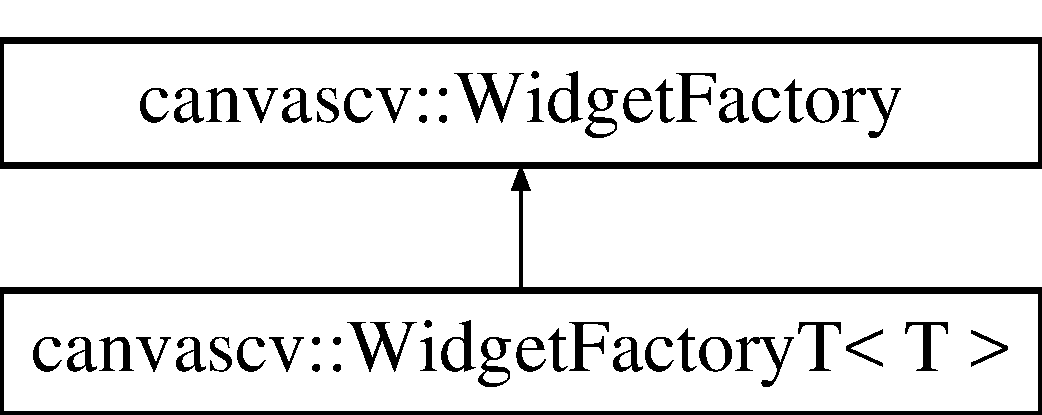
\includegraphics[height=2.000000cm]{classcanvascv_1_1WidgetFactory}
\end{center}
\end{figure}
\subsection*{Static Public Member Functions}
\begin{DoxyCompactItemize}
\item 
static std\+::shared\+\_\+ptr$<$ \hyperlink{classcanvascv_1_1Widget}{Widget} $>$ \hyperlink{classcanvascv_1_1WidgetFactory_abfde5dd5df7726be47f17a83197cb0c4}{new\+Widget} (std\+::string type, \hyperlink{classcanvascv_1_1Layout}{Layout} \&layout\+Val, const cv\+::\+Point \&pos)
\begin{DoxyCompactList}\small\item\em new\+Widget \end{DoxyCompactList}\end{DoxyCompactItemize}


\subsection{Detailed Description}
\hyperlink{classcanvascv_1_1Widget}{Widget} prototypes are added to this class with the help of the \hyperlink{classcanvascv_1_1WidgetFactoryT}{Widget\+FactoryT} class. You can create widgets with \hyperlink{classcanvascv_1_1WidgetFactory_abfde5dd5df7726be47f17a83197cb0c4}{new\+Widget()} of this class, but if you supply a wrong name you\textquotesingle{}ll get back a null pointer. \begin{Desc}
\item[Examples\+: ]\par
\hyperlink{example_add_widget_8cpp-example}{example\+\_\+add\+\_\+widget.\+cpp}.\end{Desc}


\subsection{Member Function Documentation}
\index{canvascv\+::\+Widget\+Factory@{canvascv\+::\+Widget\+Factory}!new\+Widget@{new\+Widget}}
\index{new\+Widget@{new\+Widget}!canvascv\+::\+Widget\+Factory@{canvascv\+::\+Widget\+Factory}}
\subsubsection[{\texorpdfstring{new\+Widget(std\+::string type, Layout \&layout\+Val, const cv\+::\+Point \&pos)}{newWidget(std::string type, Layout &layoutVal, const cv::Point &pos)}}]{\setlength{\rightskip}{0pt plus 5cm}static std\+::shared\+\_\+ptr$<${\bf Widget}$>$ canvascv\+::\+Widget\+Factory\+::new\+Widget (
\begin{DoxyParamCaption}
\item[{std\+::string}]{type, }
\item[{{\bf Layout} \&}]{layout\+Val, }
\item[{const cv\+::\+Point \&}]{pos}
\end{DoxyParamCaption}
)\hspace{0.3cm}{\ttfamily [static]}}\hypertarget{classcanvascv_1_1WidgetFactory_abfde5dd5df7726be47f17a83197cb0c4}{}\label{classcanvascv_1_1WidgetFactory_abfde5dd5df7726be47f17a83197cb0c4}
Use this to create widgets by name. 
\begin{DoxyParams}{Parameters}
{\em type} & is the name of the concrete \hyperlink{classcanvascv_1_1Widget}{Widget} sub type. \\
\hline
{\em layout\+Val} & is the parent layout \\
\hline
{\em pos} & is an intial location for the \hyperlink{classcanvascv_1_1Widget}{Widget} on the \hyperlink{classcanvascv_1_1Layout}{Layout} (if the layout supports specific positions). \\
\hline
\end{DoxyParams}
\begin{DoxyReturn}{Returns}
a pointer to a newly allocated widget of type \textquotesingle{}type\textquotesingle{} or nullptr if \textquotesingle{}type\textquotesingle{} doesn\textquotesingle{}t exist. 
\end{DoxyReturn}


The documentation for this class was generated from the following file\+:\begin{DoxyCompactItemize}
\item 
Canvas\+C\+V-\/doxygen/src/canvascv/widgets/widgetfactory.\+h\end{DoxyCompactItemize}

\hypertarget{classcanvascv_1_1WidgetFactoryT}{}\section{canvascv\+:\+:Widget\+FactoryT$<$ T $>$ Class Template Reference}
\label{classcanvascv_1_1WidgetFactoryT}\index{canvascv\+::\+Widget\+Factory\+T$<$ T $>$@{canvascv\+::\+Widget\+Factory\+T$<$ T $>$}}


The \hyperlink{classcanvascv_1_1WidgetFactoryT}{Widget\+FactoryT} class.  




{\ttfamily \#include $<$widgetfactory.\+h$>$}

Inheritance diagram for canvascv\+:\+:Widget\+FactoryT$<$ T $>$\+:\begin{figure}[H]
\begin{center}
\leavevmode
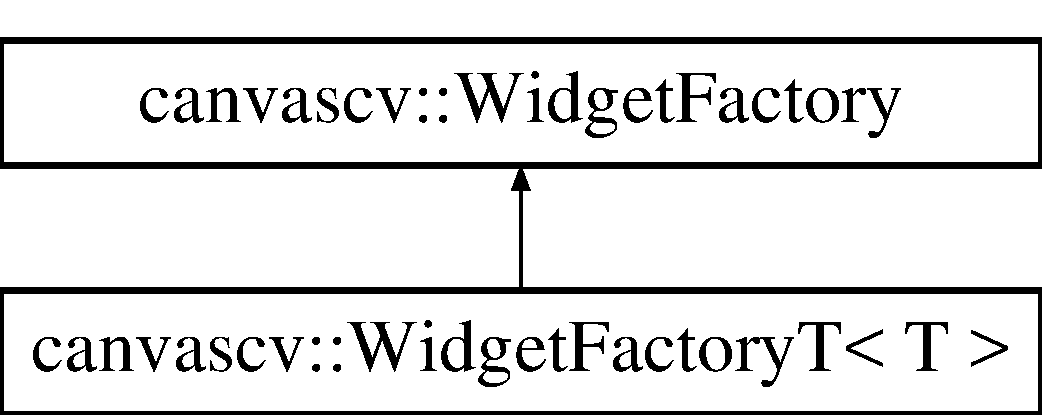
\includegraphics[height=2.000000cm]{classcanvascv_1_1WidgetFactoryT}
\end{center}
\end{figure}
\subsection*{Static Public Member Functions}
\begin{DoxyCompactItemize}
\item 
static bool \hyperlink{classcanvascv_1_1WidgetFactoryT_afc65f55a1043450975cc5431b10fbe89}{add\+Type} (std\+::string name)
\begin{DoxyCompactList}\small\item\em add\+Type adds type \textquotesingle{}T\textquotesingle{} under name \textquotesingle{}name\textquotesingle{} \end{DoxyCompactList}\item 
static std\+::shared\+\_\+ptr$<$ T $>$ \hyperlink{classcanvascv_1_1WidgetFactoryT_afa3a2961a2fdb649dacb86a07c3c26a0}{new\+Widget} (\hyperlink{classcanvascv_1_1Layout}{Layout} \&layout\+Val, const cv\+::\+Point \&pos=cv\+::\+Point(0, 0))
\begin{DoxyCompactList}\small\item\em new\+Widget \end{DoxyCompactList}\end{DoxyCompactItemize}


\subsection{Detailed Description}
\subsubsection*{template$<$class T$>$\\*
class canvascv\+::\+Widget\+Factory\+T$<$ T $>$}

This is the compile-\/time type-\/safe version of the \hyperlink{classcanvascv_1_1WidgetFactory}{Widget\+Factory}. Types added here with \hyperlink{classcanvascv_1_1WidgetFactoryT_afc65f55a1043450975cc5431b10fbe89}{add\+Type()} are guranteed to exist at compile time. Types created by \hyperlink{classcanvascv_1_1WidgetFactoryT_afa3a2961a2fdb649dacb86a07c3c26a0}{new\+Widget()} are guranteed to exist at compile time. \begin{Desc}
\item[Examples\+: ]\par
\hyperlink{example_add_widget_8cpp-example}{example\+\_\+add\+\_\+widget.\+cpp}.\end{Desc}


\subsection{Member Function Documentation}
\index{canvascv\+::\+Widget\+FactoryT@{canvascv\+::\+Widget\+FactoryT}!add\+Type@{add\+Type}}
\index{add\+Type@{add\+Type}!canvascv\+::\+Widget\+FactoryT@{canvascv\+::\+Widget\+FactoryT}}
\subsubsection[{\texorpdfstring{add\+Type(std\+::string name)}{addType(std::string name)}}]{\setlength{\rightskip}{0pt plus 5cm}template$<$class T $>$ bool {\bf canvascv\+::\+Widget\+FactoryT}$<$ T $>$\+::add\+Type (
\begin{DoxyParamCaption}
\item[{std\+::string}]{name}
\end{DoxyParamCaption}
)\hspace{0.3cm}{\ttfamily [static]}}\hypertarget{classcanvascv_1_1WidgetFactoryT_afc65f55a1043450975cc5431b10fbe89}{}\label{classcanvascv_1_1WidgetFactoryT_afc65f55a1043450975cc5431b10fbe89}

\begin{DoxyParams}{Parameters}
{\em name} & \\
\hline
\end{DoxyParams}
\begin{DoxyReturn}{Returns}
true if type \textquotesingle{}T\textquotesingle{} is registering for the first time ot false otherwise 
\end{DoxyReturn}
\begin{DoxySeeAlso}{See also}
C\+C\+V\+\_\+\+R\+E\+G\+I\+S\+T\+E\+R\+\_\+\+W\+I\+D\+G\+ET macro in Widget\+Factory.\+h 
\end{DoxySeeAlso}
\index{canvascv\+::\+Widget\+FactoryT@{canvascv\+::\+Widget\+FactoryT}!new\+Widget@{new\+Widget}}
\index{new\+Widget@{new\+Widget}!canvascv\+::\+Widget\+FactoryT@{canvascv\+::\+Widget\+FactoryT}}
\subsubsection[{\texorpdfstring{new\+Widget(\+Layout \&layout\+Val, const cv\+::\+Point \&pos=cv\+::\+Point(0, 0))}{newWidget(Layout &layoutVal, const cv::Point &pos=cv::Point(0, 0))}}]{\setlength{\rightskip}{0pt plus 5cm}template$<$class T $>$ std\+::shared\+\_\+ptr$<$ T $>$ {\bf canvascv\+::\+Widget\+FactoryT}$<$ T $>$\+::new\+Widget (
\begin{DoxyParamCaption}
\item[{{\bf Layout} \&}]{layout\+Val, }
\item[{const cv\+::\+Point \&}]{pos = {\ttfamily cv\+:\+:Point(0,0)}}
\end{DoxyParamCaption}
)\hspace{0.3cm}{\ttfamily [static]}}\hypertarget{classcanvascv_1_1WidgetFactoryT_afa3a2961a2fdb649dacb86a07c3c26a0}{}\label{classcanvascv_1_1WidgetFactoryT_afa3a2961a2fdb649dacb86a07c3c26a0}
Use this to create widgets by compile-\/time type. 
\begin{DoxyParams}{Parameters}
{\em layout\+Val} & is the parent layout \\
\hline
{\em pos} & is an intial location for the \hyperlink{classcanvascv_1_1Widget}{Widget} on the \hyperlink{classcanvascv_1_1Layout}{Layout} (if the layout supports specific positions). \\
\hline
\end{DoxyParams}
\begin{DoxyReturn}{Returns}
a pointer to a newly allocated widget of type \textquotesingle{}type\textquotesingle{}. 
\end{DoxyReturn}


The documentation for this class was generated from the following file\+:\begin{DoxyCompactItemize}
\item 
Canvas\+C\+V-\/doxygen/src/canvascv/widgets/widgetfactory.\+h\end{DoxyCompactItemize}

\chapter{Example Documentation}
\hypertarget{example_add_theme_8cpp-example}{}\section{example\+\_\+add\+\_\+theme.\+cpp}
This is an example of how to add a theme.


\begin{DoxyCodeInclude}
\textcolor{preprocessor}{#include "canvascv/canvas.h"}

\textcolor{comment}{// These are used to create widgets}
\textcolor{preprocessor}{#include "canvascv/widgets/radiobuttons.h"}
\textcolor{preprocessor}{#include "canvascv/widgets/text.h"}
\textcolor{preprocessor}{#include "canvascv/widgets/button.h"}
\textcolor{preprocessor}{#include "canvascv/widgets/hframe.h"}
\textcolor{preprocessor}{#include "canvascv/themes/themerepository.h"}
\textcolor{preprocessor}{#include "canvascv/themes/twocoloredtheme.h"}

\textcolor{preprocessor}{#include <iostream>}
\textcolor{preprocessor}{#include <iterator>}

\textcolor{preprocessor}{#include <opencv2/highgui.hpp>}

\textcolor{keyword}{using namespace }\hyperlink{namespacestd}{std};
\textcolor{keyword}{using namespace }\hyperlink{namespacecv}{cv};
\textcolor{keyword}{using namespace }\hyperlink{namespacecanvascv}{canvascv};

\textcolor{keyword}{class }MyTheme : \textcolor{keyword}{public} \hyperlink{classcanvascv_1_1TwoColoredTheme}{TwoColoredTheme}
\{
\textcolor{keyword}{public}:
    MyTheme(Scalar fgColor, Scalar bgColor, \textcolor{keywordtype}{int} widthVal)
        : \hyperlink{classcanvascv_1_1TwoColoredTheme}{TwoColoredTheme}(fgColor, bgColor),
          width(widthVal)
    \{\}

    \textcolor{keyword}{virtual} \textcolor{keywordtype}{void} allocateBG(Mat &dst, \textcolor{keyword}{const} Size &size, \textcolor{keyword}{const} Scalar &color)
    \{
        TwoColoredTheme::allocateBG(dst, size, color);
        \textcolor{keywordflow}{if} (! dst.empty())
        \{
            Point pFrom(0,0);
            Point pTo(0,size.height);
            \textcolor{keywordtype}{int} spacing = width * 2;
            \textcolor{keywordflow}{for} (pFrom.x = 0, pTo.x = pFrom.x - size.height ; pTo.x < size.width; pFrom.x += spacing, pTo.x
       += spacing)
            \{
                cv::line(dst, pFrom, pTo, color*1.5, width, LINE\_AA);
            \}
        \}
    \}
\textcolor{keyword}{private}:
    \textcolor{keywordtype}{int} width;
\};

\textcolor{keywordtype}{int} main(\textcolor{keywordtype}{int} argc, \textcolor{keywordtype}{char} **argv)
\{
    --argc;
    ++argv;
    Mat image;
    \textcolor{keywordflow}{if} (argc)
    \{
        Mat orig = imread(argv[0]);
        \textcolor{keywordflow}{if} (orig.empty())
        \{
            Canvas::fatal(\textcolor{keywordtype}{string}(\textcolor{stringliteral}{"Cannot load image "}) + argv[0], -1);
        \}
        \textcolor{keywordflow}{if} (orig.cols > 1024)
        \{
            \textcolor{keywordtype}{double} ratio = 1024. / orig.cols;
            cv::resize(orig, image, Size(), ratio, ratio);
        \}
        \textcolor{keywordflow}{else}
        \{
            image = orig;
        \}
    \}
    \textcolor{keywordflow}{else}
    \{
        Canvas::fatal(\textcolor{stringliteral}{"Must get a path to an image as a parameter"} , -1);
    \}

    \hyperlink{classcanvascv_1_1Canvas}{Canvas} c(\textcolor{stringliteral}{"Canvas"}, image.size());
    \textcolor{keyword}{auto} layout = HFrame::create(c, Point(5, image.rows / 2.));
    \hyperlink{classcanvascv_1_1Widget_a977cbd39cf203c5866f07f3645c7e4bc}{Widget::CBUserSelection} cb = [&c, &layout](\hyperlink{classcanvascv_1_1Widget}{Widget} *w, \textcolor{keywordtype}{int} index) \{
        \hyperlink{classcanvascv_1_1RadioButtons}{RadioButtons} *rb = (\hyperlink{classcanvascv_1_1RadioButtons}{RadioButtons}*)w;
        \textcolor{keywordtype}{string} themeName = rb->\hyperlink{classcanvascv_1_1RadioButtons_a6a1570cb5b8328fba59bb0c17f63debc}{getTextAt}(index);
        ThemeRepository::setCurrentTheme(themeName);
        c.applyTheme();
        layout->at<\hyperlink{classcanvascv_1_1Text}{Text}>(0)->setText(CCV\_STR(\textcolor{stringliteral}{"User selected theme '"} << index << \textcolor{stringliteral}{"': '"} << themeName <<
       \textcolor{stringliteral}{"'\(\backslash\)n"}));
    \};

    ThemeRepository::addTheme(\textcolor{stringliteral}{"MyTheme1"}, \textcolor{keyword}{new} MyTheme(Colors::Red, Colors::Pink, 10));
    ThemeRepository::addTheme(\textcolor{stringliteral}{"MyTheme2"}, \textcolor{keyword}{new} MyTheme(Colors::Red, Colors::Pink, 20));
    ThemeRepository::addTheme(\textcolor{stringliteral}{"MyTheme3"}, \textcolor{keyword}{new} MyTheme(Colors::Blue, Colors::Green, 20));
    vector<string> availThemes = ThemeRepository::availThemes();

    \textcolor{keyword}{auto} iter = std::find(availThemes.begin(), availThemes.end(), ThemeRepository::getCurrentThemeName());
    \textcolor{keywordtype}{int} i = std::distance(availThemes.begin(), iter);

    \textcolor{keyword}{auto} text = Text::create(*layout, \textcolor{stringliteral}{""}, Widget::TOP, Widget::CENTER);
    text->setMaxWidth(100);
    text->setAlpha(0);
    RadioButtons::create(*layout, availThemes, i, cb);
    Button::create(*layout, \textcolor{stringliteral}{"First button"})->setLayoutAnchor(Widget::CENTER);
    Button::create(*layout, \textcolor{stringliteral}{"Second button"})->setLayoutAnchor(Widget::CENTER);

    namedWindow(\textcolor{stringliteral}{"Canvas"}, WINDOW\_AUTOSIZE);
    c.setMouseCallback(); \textcolor{comment}{// optional for mouse usage see also (example\_selectbox.cpp)}

    \textcolor{keywordtype}{int} key = 0;
    Mat out; \textcolor{comment}{// keeping it out of the loop is a little more efficient}
    \textcolor{keywordflow}{while} (key != \textcolor{charliteral}{'q'})
    \{
        c.redrawOn(image, out);
        imshow(\textcolor{stringliteral}{"Canvas"}, out);
        key = c.waitKeyEx(); \textcolor{comment}{// GUI and callbacks happen here}
    \}

    destroyAllWindows();
    \textcolor{keywordflow}{return} 0;
\}


\end{DoxyCodeInclude}
 
\hypertarget{example_add_widget_8cpp-example}{}\section{example\+\_\+add\+\_\+widget.\+cpp}
This is an example of how to add a widget.


\begin{DoxyCodeInclude}
\textcolor{preprocessor}{#include "canvascv/canvas.h"}

\textcolor{comment}{// These are used to create widgets}
\textcolor{preprocessor}{#include "canvascv/widgets/text.h"}
\textcolor{preprocessor}{#include "canvascv/widgets/button.h"}
\textcolor{preprocessor}{#include "canvascv/widgets/hframe.h"}
\textcolor{preprocessor}{#include "canvascv/widgets/vframe.h"}
\textcolor{preprocessor}{#include "canvascv/widgets/widgetfactory.h"}

\textcolor{preprocessor}{#include <iostream>}

\textcolor{preprocessor}{#include <opencv2/highgui.hpp>}

\textcolor{comment}{// This was integrated into c++17, but experimental in c++11,}
\textcolor{comment}{//  which is currently our minimum version}
\textcolor{preprocessor}{#include <experimental/filesystem>}
\textcolor{keyword}{namespace }fs = std::experimental::filesystem;

\textcolor{keyword}{using namespace }\hyperlink{namespacestd}{std};
\textcolor{keyword}{using namespace }\hyperlink{namespacecv}{cv};
\textcolor{keyword}{using namespace }\hyperlink{namespacecanvascv}{canvascv};

\textcolor{keyword}{class }FileBrowser : \textcolor{keyword}{public} \hyperlink{classcanvascv_1_1CompoundWidget}{CompoundWidget}
\{
\textcolor{keyword}{public}:
    \textcolor{keyword}{static} std::shared\_ptr<FileBrowser> create(\hyperlink{classcanvascv_1_1Layout}{Layout} &layoutVal,
                                               \textcolor{keyword}{const} std::string &startPath,
                                               \hyperlink{classcanvascv_1_1Widget_a977cbd39cf203c5866f07f3645c7e4bc}{Widget::CBUserSelection} 
      cbUserSelection = \hyperlink{classcanvascv_1_1Widget_a977cbd39cf203c5866f07f3645c7e4bc}{Widget::CBUserSelection}(),
                                               \textcolor{keyword}{const} cv::Point &pos = cv::Point(-1,-1))
    \{
        shared\_ptr<FileBrowser> fb = \hyperlink{classcanvascv_1_1WidgetFactoryT}{WidgetFactoryT<FileBrowser>::newWidget}
      (layoutVal, pos);
        fb->setCurrentPath(startPath);
        fb->userCB = cbUserSelection;
        \textcolor{keywordflow}{return} fb;
    \}

    \textcolor{keywordtype}{string} getCurrentPath()\textcolor{keyword}{ const}
\textcolor{keyword}{    }\{
        \textcolor{keywordflow}{return} currentPath;
    \}

    \textcolor{keywordtype}{void} setCurrentPath(\textcolor{keyword}{const} \textcolor{keywordtype}{string} &value)
    \{
        \textcolor{keywordflow}{if} (currentPath != value)
        \{
            currentPath = value;
            setDirty();
        \}
    \}

    \textcolor{keyword}{virtual} \textcolor{keyword}{const} \textcolor{keywordtype}{char} *getType()\textcolor{keyword}{ const }\{\textcolor{keywordflow}{return} type;\}
    \textcolor{keyword}{static} \textcolor{keyword}{const} \textcolor{keywordtype}{char} *type;

    \textcolor{keywordtype}{string} getUserSelection()\textcolor{keyword}{ const}
\textcolor{keyword}{    }\{
        \textcolor{keywordflow}{return} userSelection;
    \}

\textcolor{keyword}{protected}:
    \textcolor{keyword}{friend} \textcolor{keyword}{class }\hyperlink{classcanvascv_1_1WidgetFactory}{canvascv::WidgetFactory};
    \textcolor{keyword}{template} <\textcolor{keyword}{class} T> \textcolor{keyword}{friend} \textcolor{keyword}{class }\hyperlink{classcanvascv_1_1WidgetFactoryT}{canvascv::WidgetFactoryT};

    FileBrowser(\textcolor{keyword}{const} cv::Point &pos)
        : \hyperlink{classcanvascv_1_1CompoundWidget}{CompoundWidget}(pos)
    \{
        top = \hyperlink{classcanvascv_1_1VFrame_a013de150c59b8f7f37aa21ac59d78b10}{VFrame::create}(*\textcolor{keyword}{this}, pos).get(); \textcolor{comment}{// note the get()}
        top->setFrameRelief(RAISED);
        top->setPadding(5);
        pathFrame = \hyperlink{classcanvascv_1_1HFrame_a0bd1d3df07a8c25f48e79048913f85fc}{HFrame::create}(*top).get(); \textcolor{comment}{// note the get()}
        pathFrame->setFrameRelief(Widget::SELECTED);
        pathFrame->setWrap(\textcolor{keyword}{true});
        filesFrame = \hyperlink{classcanvascv_1_1HFrame_a0bd1d3df07a8c25f48e79048913f85fc}{HFrame::create}(*top).get(); \textcolor{comment}{// note the get()}
        filesFrame->setFrameRelief(Widget::SELECTED);
        filesFrame->setWrap(\textcolor{keyword}{true});
        \textcolor{keyword}{auto} okCancel = \hyperlink{classcanvascv_1_1HorizontalLayout_aea31dd787cbf985687ead6a55efa1839}{HorizontalLayout::create}(*top);
        okCancel->setLayoutAnchor(CENTER);
        \hyperlink{classcanvascv_1_1Button_a3557ea02dfca8d6cb92181a2d2b88112}{Button::create}(*okCancel, \textcolor{stringliteral}{"Cancel"}, \textcolor{stringliteral}{""}, [\textcolor{keyword}{this}](\hyperlink{classcanvascv_1_1Widget}{Widget}*) \{rmvFromLayout();\});
        \hyperlink{classcanvascv_1_1Button_a3557ea02dfca8d6cb92181a2d2b88112}{Button::create}(*okCancel, \textcolor{stringliteral}{"Ok"}, \textcolor{stringliteral}{""}, [\textcolor{keyword}{this}](\hyperlink{classcanvascv_1_1Widget}{Widget}*)
        \{
            userSelection = currentPath;
            \textcolor{keywordflow}{if} (userCB) userCB(\textcolor{keyword}{this}, 0);
            rmvFromLayout();
        \});
    \}

    \textcolor{keyword}{virtual} \textcolor{keywordtype}{void} recalcCompound()
    \{
        fs::path pathObj(getCurrentPath());
        \textcolor{keywordflow}{if} (fs::is\_directory(pathObj) &&
                currentDir != pathObj.string())
        \{
            \textcolor{keywordflow}{for} (\textcolor{keyword}{auto} f : files) \{ f->rmvFromLayout(); \}
            files.clear();
            currentDir = pathObj.string();
            \textcolor{keywordflow}{for}(\textcolor{keyword}{auto}& p: fs::directory\_iterator(getCurrentPath()))
            \{
                \textcolor{keywordflow}{if} (fs::is\_directory(p))
                \{
                    \hyperlink{classcanvascv_1_1Button}{Button} *dir = \hyperlink{classcanvascv_1_1Button_a3557ea02dfca8d6cb92181a2d2b88112}{Button::create}(*filesFrame, p.path().filename().
      string()).\textcolor{keyword}{get}();
                    dir->\hyperlink{classcanvascv_1_1Widget_abdb1aed0ca76845ba6a56c4f8db502c9}{notifyOnChange}([\textcolor{keyword}{this}, p](\hyperlink{classcanvascv_1_1Widget}{Widget} *, 
      \hyperlink{classcanvascv_1_1Widget_afc39a6533455cbc3161ae3a021da0dc8}{Widget::State} state) \{
                        \textcolor{keywordflow}{if} (state == \hyperlink{classcanvascv_1_1Widget_afc39a6533455cbc3161ae3a021da0dc8abb395c6efa7fc11a3176d1f801bdbc86}{Widget::PRESS}) \{
                            setCurrentPath(p.path().string());
                        \}
                    \});
                    files.push\_back(dir);
                \}
                \textcolor{keywordflow}{else}
                \{
                    \hyperlink{classcanvascv_1_1Button}{Button} *file = \hyperlink{classcanvascv_1_1Button_a3557ea02dfca8d6cb92181a2d2b88112}{Button::create}(*filesFrame, p.path().filename().
      string()).\textcolor{keyword}{get}();
                    file->\hyperlink{classcanvascv_1_1Button_a7d2c79daa9d22bf02c2cc978ff10df7e}{setFlatButton}();
                    file->\hyperlink{classcanvascv_1_1Widget_abdb1aed0ca76845ba6a56c4f8db502c9}{notifyOnChange}([\textcolor{keyword}{this}, p](\hyperlink{classcanvascv_1_1Widget}{Widget} *, 
      \hyperlink{classcanvascv_1_1Widget_afc39a6533455cbc3161ae3a021da0dc8}{Widget::State} state) \{
                        \textcolor{keywordflow}{if} (state == \hyperlink{classcanvascv_1_1Widget_afc39a6533455cbc3161ae3a021da0dc8abb395c6efa7fc11a3176d1f801bdbc86}{Widget::PRESS}) \{
                            setCurrentPath(p.path().string());
                        \}
                    \});
                    files.push\_back(file);
                \}
            \}
        \}
        \textcolor{keywordflow}{for} (\textcolor{keyword}{auto} b : path) \{ b->rmvFromLayout(); \}
        path.clear();
        list<fs::path> parts;
        \textcolor{keywordflow}{do}
        \{
            parts.push\_front(pathObj);
            pathObj = pathObj.parent\_path();
        \} \textcolor{keywordflow}{while} (pathObj.string().length());
        \textcolor{keywordflow}{for} (\textcolor{keyword}{auto} &p : parts)
        \{
            \textcolor{keywordflow}{if} (fs::is\_directory(p))
            \{
                \hyperlink{classcanvascv_1_1Button}{Button} *dir = \hyperlink{classcanvascv_1_1Button_a3557ea02dfca8d6cb92181a2d2b88112}{Button::create}(*pathFrame, p.filename().string()).\textcolor{keyword}{get}();
                dir->\hyperlink{classcanvascv_1_1Widget_abdb1aed0ca76845ba6a56c4f8db502c9}{notifyOnChange}([\textcolor{keyword}{this}, p](\hyperlink{classcanvascv_1_1Widget}{Widget} *, 
      \hyperlink{classcanvascv_1_1Widget_afc39a6533455cbc3161ae3a021da0dc8}{Widget::State} state) \{
                    \textcolor{keywordflow}{if} (state == \hyperlink{classcanvascv_1_1Widget_afc39a6533455cbc3161ae3a021da0dc8abb395c6efa7fc11a3176d1f801bdbc86}{Widget::PRESS}) \{
                        setCurrentPath(p.string());
                    \}
                \});
                path.push\_back(dir);
            \}
            \textcolor{keywordflow}{else}
            \{
                \hyperlink{classcanvascv_1_1Button}{Button} *file = \hyperlink{classcanvascv_1_1Button_a3557ea02dfca8d6cb92181a2d2b88112}{Button::create}(*pathFrame, p.filename().string()).\textcolor{keyword}{get}();
                file->\hyperlink{classcanvascv_1_1Button_a7d2c79daa9d22bf02c2cc978ff10df7e}{setFlatButton}();
                path.push\_back(file);
            \}
        \}
        top->update(); \textcolor{comment}{// Since we're making widgets dirty in recalc*() we need to manually update them}
        recalcRect(0);
    \}

\textcolor{keyword}{private}:
    CBUserSelection userCB;
    fs::path currentDir;
    \textcolor{keywordtype}{string} currentPath;
    \textcolor{keywordtype}{string} userSelection;

    \textcolor{comment}{// It's enough to keep pointers.}
    \textcolor{comment}{// The layout is holding the smart pointers,}
    \textcolor{comment}{//  and that's keeping the reference count up.}
    \hyperlink{classcanvascv_1_1VFrame}{VFrame} *top;
    \hyperlink{classcanvascv_1_1HFrame}{HFrame} *pathFrame;
    list<Button*> path;
    \hyperlink{classcanvascv_1_1HFrame}{HFrame} *filesFrame;
    list<Button*> files;
\};
\textcolor{keyword}{const} \textcolor{keywordtype}{char} *FileBrowser::type = \textcolor{stringliteral}{"FileBrowser"};

CCV\_REGISTER\_WIDGET(FileBrowser);

\textcolor{keyword}{static} Mat readImg(\textcolor{keyword}{const} \textcolor{keywordtype}{string} &name)
\{
    Mat image;
    Mat orig = imread(name, IMREAD\_UNCHANGED);
    \textcolor{keywordflow}{if} (! orig.empty())
    \{
        \textcolor{keywordflow}{if} (orig.cols > 1024)
        \{
            \textcolor{keywordtype}{double} ratio = 1024. / orig.cols;
            cv::resize(orig, image, Size(), ratio, ratio);
        \}
        \textcolor{keywordflow}{else}
        \{
            image = orig;
        \}
    \}
    \textcolor{keywordflow}{return} image;
\}

\textcolor{keywordtype}{int} main(\textcolor{keywordtype}{int} argc, \textcolor{keywordtype}{char} **argv)
\{
    --argc;
    ++argv;
    Mat image;
    \textcolor{keywordflow}{if} (argc)
    \{
        image = readImg(argv[0]);
        \textcolor{keywordflow}{if} (image.empty())
        \{
            \hyperlink{classcanvascv_1_1Canvas_add93c0d5cc1e9b49f97510952a8a1961}{Canvas::fatal}(\textcolor{keywordtype}{string}(\textcolor{stringliteral}{"Cannot load image "}) + argv[0], -1);
        \}
    \}
    \textcolor{keywordflow}{else}
    \{
        \hyperlink{classcanvascv_1_1Canvas_add93c0d5cc1e9b49f97510952a8a1961}{Canvas::fatal}(\textcolor{stringliteral}{"Must get a path to an image as a parameter"} , -1);
    \}

    fs::path startPath(argv[0]);
    startPath = startPath.parent\_path();

    \hyperlink{classcanvascv_1_1Canvas}{Canvas} c(\textcolor{stringliteral}{"Canvas"}, image.size());

    namedWindow(\textcolor{stringliteral}{"Canvas"}, WINDOW\_AUTOSIZE);
    c.setMouseCallback(); \textcolor{comment}{// optional for mouse usage see also (example\_selectbox.cpp)}

    shared\_ptr<FileBrowser> fb;
    \hyperlink{classcanvascv_1_1Widget_a977cbd39cf203c5866f07f3645c7e4bc}{Widget::CBUserSelection} cb = [&c, &image](\hyperlink{classcanvascv_1_1Widget}{Widget} *w, int)
    \{
        cout << \textcolor{stringliteral}{"CB: Got user selection '"} << ((FileBrowser*)w)->getUserSelection() << \textcolor{stringliteral}{"'"} << endl;
        Mat tmp = readImg(((FileBrowser*)w)->getUserSelection());
        \textcolor{keywordflow}{if} (tmp.empty())
        \{
            cout << \textcolor{stringliteral}{"OpenCV cannot read this image"} << endl;
        \}
        \textcolor{keywordflow}{else}
        \{
            image = tmp;
            c.setSize(image.size());
        \}
    \};

    \textcolor{keywordtype}{int} delay = 1000/25; \textcolor{comment}{// if using a polling API we need a delay}
    \textcolor{keywordtype}{int} key = 0;
    Mat out; \textcolor{comment}{// keeping it out of the loop is a little more efficient}
    \textcolor{keywordflow}{while} (key != \textcolor{charliteral}{'q'})
    \{
        \textcolor{keywordflow}{if} (! fb)
        \{
            fb = FileBrowser::create(c, startPath.string(), cb);
            fb->setFillColor(\hyperlink{classcanvascv_1_1Colors_acabb2042568dac2c0fbefcc92b48be0b}{Colors::RoyalBlue});
            fb->setAlpha(128);
        \}
        c.redrawOn(image, out);
        imshow(\textcolor{stringliteral}{"Canvas"}, out);
        key = c.waitKeyEx(delay); \textcolor{comment}{// GUI and callbacks happen here}
        \textcolor{keywordflow}{if} (fb->getUserSelection().length())
        \{
            cout << \textcolor{stringliteral}{"Loop: Got user selection '"} << fb->getUserSelection() << \textcolor{stringliteral}{"'"} << endl;
            cout << \textcolor{stringliteral}{"Starting a new FileBrowser"} << endl;
            startPath = fb->getUserSelection();
            \textcolor{keywordflow}{if} (! fs::is\_directory(startPath)) startPath = startPath.parent\_path();
            fb = FileBrowser::create(c, startPath.string(), cb);
            fb->setFillColor(\hyperlink{classcanvascv_1_1Colors_acabb2042568dac2c0fbefcc92b48be0b}{Colors::RoyalBlue});
            fb->setAlpha(128);
        \}
        \textcolor{keywordflow}{if} (fb->isRemoved() && ! fb->getUserSelection().length())
        \{
            cout << \textcolor{stringliteral}{"User canceled"} << endl;
            \textcolor{keywordflow}{break};
        \}
    \}

    destroyAllWindows();
    \textcolor{keywordflow}{return} 0;
\}
\end{DoxyCodeInclude}
 
\hypertarget{example_checkboxes_8cpp-example}{}\section{example\+\_\+checkboxes.\+cpp}
This is an example of how to use the Check\+Boxes Widget.


\begin{DoxyCodeInclude}
\textcolor{preprocessor}{#include "canvascv/canvas.h"}

\textcolor{comment}{// These are used to create widgets}
\textcolor{preprocessor}{#include "canvascv/widgets/checkboxes.h"}

\textcolor{preprocessor}{#include <iostream>}
\textcolor{preprocessor}{#include <iterator>}

\textcolor{preprocessor}{#include <opencv2/highgui.hpp>}

\textcolor{keyword}{using namespace }\hyperlink{namespacestd}{std};
\textcolor{keyword}{using namespace }\hyperlink{namespacecv}{cv};
\textcolor{keyword}{using namespace }\hyperlink{namespacecanvascv}{canvascv};

\textcolor{keywordtype}{int} main(\textcolor{keywordtype}{int} argc, \textcolor{keywordtype}{char} **argv)
\{
    --argc;
    ++argv;
    Mat image;
    \textcolor{keywordflow}{if} (argc)
    \{
        Mat orig = imread(argv[0]);
        \textcolor{keywordflow}{if} (orig.empty())
        \{
            \hyperlink{classcanvascv_1_1Canvas_add93c0d5cc1e9b49f97510952a8a1961}{Canvas::fatal}(\textcolor{keywordtype}{string}(\textcolor{stringliteral}{"Cannot load image "}) + argv[0], -1);
        \}
        \textcolor{keywordflow}{if} (orig.cols > 1024)
        \{
            \textcolor{keywordtype}{double} ratio = 1024. / orig.cols;
            cv::resize(orig, image, Size(), ratio, ratio);
        \}
        \textcolor{keywordflow}{else}
        \{
            image = orig;
        \}
    \}
    \textcolor{keywordflow}{else}
    \{
        \hyperlink{classcanvascv_1_1Canvas_add93c0d5cc1e9b49f97510952a8a1961}{Canvas::fatal}(\textcolor{stringliteral}{"Must get a path to an image as a parameter"} , -1);
    \}

    \hyperlink{classcanvascv_1_1Canvas}{Canvas} c(\textcolor{stringliteral}{"Canvas"}, image.size());
    c.\hyperlink{classcanvascv_1_1Canvas_ae68d3277e738d349232400b38f0e5f9e}{enableScreenText}();
    c.setScreenText(\textcolor{stringliteral}{"Nothing selected"});
    \hyperlink{classcanvascv_1_1Widget_a977cbd39cf203c5866f07f3645c7e4bc}{Widget::CBUserSelection} cb = [&c](\hyperlink{classcanvascv_1_1Widget}{Widget} *w, \textcolor{keywordtype}{int} index) \{
        stringstream s;
        \hyperlink{classcanvascv_1_1CheckBoxes}{CheckBoxes} *boxes = (\hyperlink{classcanvascv_1_1CheckBoxes}{CheckBoxes}*)w;
        s << \textcolor{stringliteral}{"User selected option '"} << index << \textcolor{stringliteral}{"': '"} << boxes->\hyperlink{classcanvascv_1_1CheckBoxes_a1ca004ddd840090415924b1f79b2ee47}{getTextAt}(index) << \textcolor{stringliteral}{"'\(\backslash\)n"};
        \textcolor{keywordflow}{for} (\textcolor{keywordtype}{int} i = 0; i < boxes->\hyperlink{classcanvascv_1_1CheckBoxes_ac2e93b64ec078504230c7330d068248c}{size}(); ++i)
            s << \textcolor{stringliteral}{"Option '"} << boxes->\hyperlink{classcanvascv_1_1CheckBoxes_a1ca004ddd840090415924b1f79b2ee47}{getTextAt}(i) << \textcolor{stringliteral}{"' is "} << boxes->
      \hyperlink{classcanvascv_1_1CheckBoxes_a2e544c7f81248c6b297460be5852506e}{isChecked}(i) << \textcolor{stringliteral}{"\(\backslash\)n"};
        c.setScreenText(s.str());
    \};

    \hyperlink{classcanvascv_1_1CheckBoxes_a5108f52385a5cb19ad7fe52a18a91df0}{CheckBoxes::create}(c, \{
                           \textcolor{stringliteral}{"One"},  \textcolor{comment}{// index 0}
                           \textcolor{stringliteral}{"Two"}, \textcolor{comment}{// index 1}
                           \textcolor{stringliteral}{"Three"},   \textcolor{comment}{// index 2}
                           \textcolor{stringliteral}{"Four"}   \textcolor{comment}{// index 3}
                       \}, cb,
                       Point(image.cols / 2., image.rows / 2.));

    namedWindow(\textcolor{stringliteral}{"Canvas"}, WINDOW\_AUTOSIZE);
    c.setMouseCallback(); \textcolor{comment}{// optional for mouse usage see also (example\_selectbox.cpp)}

    \textcolor{keywordtype}{int} key = 0;
    Mat out; \textcolor{comment}{// keeping it out of the loop is a little more efficient}
    \textcolor{keywordflow}{while} (key != \textcolor{charliteral}{'q'})
    \{
        c.redrawOn(image, out);
        imshow(\textcolor{stringliteral}{"Canvas"}, out);
        key = c.waitKeyEx(); \textcolor{comment}{// GUI and callbacks happen here}
    \}

    destroyAllWindows();
    \textcolor{keywordflow}{return} 0;
\}
\end{DoxyCodeInclude}
 
\hypertarget{example_linecrossing_8cpp-example}{}\section{example\+\_\+linecrossing.\+cpp}
This is an example of how to use the Line\+Crossing shape.


\begin{DoxyCodeInclude}
\textcolor{comment}{// Mandator include file}
\textcolor{preprocessor}{#include "canvascv/canvas.h"}

\textcolor{comment}{// We need specific linecrossing and arrow features here}
\textcolor{preprocessor}{#include "canvascv/shapes/linecrossing.h"}
\textcolor{preprocessor}{#include "canvascv/shapes/arrow.h"}

\textcolor{preprocessor}{#include <iostream>}
\textcolor{preprocessor}{#include <iterator>}

\textcolor{preprocessor}{#include <opencv2/highgui.hpp>}

\textcolor{keyword}{using namespace }\hyperlink{namespacestd}{std};
\textcolor{keyword}{using namespace }\hyperlink{namespacecv}{cv};
\textcolor{keyword}{using namespace }\hyperlink{namespacecanvascv}{canvascv};

\textcolor{keyword}{static} \textcolor{keywordtype}{string} gHelpMsg =
\textcolor{stringliteral}{"Usage:\(\backslash\)n"}
\textcolor{stringliteral}{"=====\(\backslash\)n"}
\textcolor{stringliteral}{"Use the mouse and keyboard.\(\backslash\)n"}
\textcolor{stringliteral}{"Click and drag to create and drag arrows\(\backslash\)n"}
\textcolor{stringliteral}{"acrooss the LineCrossing.\(\backslash\)n"}
\textcolor{stringliteral}{"Change the LineCrossing direction and\(\backslash\)n"}
\textcolor{stringliteral}{"create/drag the arrows again.\(\backslash\)n"}
\textcolor{stringliteral}{"Use these keys:\(\backslash\)n"}
\textcolor{stringliteral}{"h: toggle usage message\(\backslash\)n"}
\textcolor{stringliteral}{"DEL: delete active shape (deleting the\(\backslash\)n"}
\textcolor{stringliteral}{"LineCrossing will exit)\(\backslash\)n"}
\textcolor{stringliteral}{"q: exit"};

\textcolor{keywordtype}{void} help(\hyperlink{classcanvascv_1_1Canvas}{Canvas} &c)
\{
    \textcolor{keyword}{static} \textcolor{keywordtype}{bool} showHelp = \textcolor{keyword}{true};
    \textcolor{keywordflow}{if} (showHelp)
    \{
        cout << gHelpMsg << endl;
        c.\hyperlink{classcanvascv_1_1Canvas_aaedea276b82a8a4cfc0895ae81113cfd}{setScreenText}(gHelpMsg);
    \}
    \textcolor{keywordflow}{else}
    \{
        c.\hyperlink{classcanvascv_1_1Canvas_aaedea276b82a8a4cfc0895ae81113cfd}{setScreenText}(\textcolor{stringliteral}{""});
    \}
    showHelp = ! showHelp;
\}

\textcolor{keywordtype}{void} setArrowColors(\hyperlink{classcanvascv_1_1LineCrossing}{LineCrossing} &lc, \hyperlink{classcanvascv_1_1Arrow}{Arrow} &arrow, Scalar defaultColor)
\{
    \hyperlink{classcanvascv_1_1Handle}{Handle} &tail = arrow.\hyperlink{classcanvascv_1_1Line_a685abcca89d05c63186ef71c0ef8b0a2}{getPT1}();
    \hyperlink{classcanvascv_1_1Handle}{Handle} &head = arrow.\hyperlink{classcanvascv_1_1Line_a7a0fc9d06ab0fc575b1596068dff0484}{getPT2}();
    \textcolor{keywordtype}{int} crossing = lc.\hyperlink{classcanvascv_1_1LineCrossing_a940cbb0be9bea9acbd82493916b1b3d6}{isCrossedBySegment}(tail(), head());
    \textcolor{keywordflow}{switch} (crossing)
    \{
    \textcolor{keywordflow}{case} 1:
        arrow.\hyperlink{classcanvascv_1_1CompoundShape_a5b01540c58f0bb5d5a7feccfa38568f9}{setOutlineColor}(\hyperlink{classcanvascv_1_1Colors_a93c492d5ea68350ee63d5b91315b5ea7}{Colors::Green});
        \textcolor{keywordflow}{break};
    \textcolor{keywordflow}{case} -1:
        arrow.\hyperlink{classcanvascv_1_1CompoundShape_a5b01540c58f0bb5d5a7feccfa38568f9}{setOutlineColor}(\hyperlink{classcanvascv_1_1Colors_a10aff24c53edf45b038d0636b061f9c2}{Colors::Red});
        \textcolor{keywordflow}{break};
    \textcolor{keywordflow}{default}:
        arrow.\hyperlink{classcanvascv_1_1CompoundShape_a5b01540c58f0bb5d5a7feccfa38568f9}{setOutlineColor}(defaultColor);
        \textcolor{keywordflow}{break};
    \}
\}

\textcolor{keywordtype}{int} main(\textcolor{keywordtype}{int} argc, \textcolor{keywordtype}{char} **argv)
\{
    --argc;
    ++argv;
    Mat image;
    \textcolor{keywordflow}{if} (argc)
    \{
        Mat orig = imread(argv[0], IMREAD\_UNCHANGED);
        \textcolor{keywordflow}{if} (orig.empty())
        \{
            \hyperlink{classcanvascv_1_1Canvas_add93c0d5cc1e9b49f97510952a8a1961}{Canvas::fatal}(\textcolor{keywordtype}{string}(\textcolor{stringliteral}{"Cannot load image "}) + argv[0], -1);
        \}
        \textcolor{keywordflow}{if} (orig.cols > 1024)
        \{
            \textcolor{keywordtype}{double} ratio = 1024. / orig.cols;
            cv::resize(orig, image, Size(), ratio, ratio);
        \}
        \textcolor{keywordflow}{else}
        \{
            image = orig;
        \}
    \}
    \textcolor{keywordflow}{else}
    \{
        image.create(600, 800, CV\_8UC3);
        image = \hyperlink{classcanvascv_1_1Colors_a79938bbb8f85fc8c8aa34a7934890c08}{Colors::White};
    \}

    \hyperlink{classcanvascv_1_1Canvas}{Canvas} c(\textcolor{stringliteral}{"Canvas"}, image.size());
    c.\hyperlink{classcanvascv_1_1Canvas_ac61735c6f4cb6a88d84331540ab25d39}{setShapeType}(\textcolor{stringliteral}{"Arrow"}); \textcolor{comment}{// default shape type for direct GUI creation}
    c.enableScreenText();
    c.enableStatusMsg();
    help(c);

    \textcolor{comment}{// create the line-crossing}
    shared\_ptr<LineCrossing> lc = c.createShape<\hyperlink{classcanvascv_1_1LineCrossing}{LineCrossing}>();
    lc->\hyperlink{classcanvascv_1_1LineCrossing_a9ee35848f19c6841cc59a373726ba8dc}{getLine}()->\hyperlink{classcanvascv_1_1Line_a51eccef05df0ea69f99ee9eca3f3b12c}{setTailPos}(Point(image.cols / 2, image.rows * 0.75));
    lc->getLine()->setHeadPos(Point(image.cols / 2, image.cols * 0.25));

    \textcolor{comment}{// notifyOnCreate callbacks can be used for many things.}
    \textcolor{comment}{// Here we bind Arrow modificatons and LineCrossing modifications}
    \textcolor{comment}{// to call setArrowColors()}
    c.notifyOnShapeCreate([lc, &c](\hyperlink{classcanvascv_1_1Shape}{Shape} *arrowShape)
    \{
        \textcolor{keywordflow}{if} (arrowShape->\hyperlink{classcanvascv_1_1Shape_adee3cc696c7e82b0d2946e7e667ddd46}{getType}() == Arrow::type)
        \{
            \hyperlink{classcanvascv_1_1Arrow}{Arrow} *arrow = (\hyperlink{classcanvascv_1_1Arrow}{Arrow}*) arrowShape;
            Scalar defaultColor = arrowShape->\hyperlink{classcanvascv_1_1Shape_a67d3bdec3be2a29c3612c87208589838}{getOutlineColor}();
            setArrowColors(*lc, *arrow, defaultColor);
            Handle::PosChangedCB cb = [arrow, defaultColor, lc](\textcolor{keyword}{const} Point&)
            \{
                setArrowColors(*lc, *arrow, defaultColor);
            \};
            arrow->\hyperlink{classcanvascv_1_1Line_a685abcca89d05c63186ef71c0ef8b0a2}{getPT1}().\hyperlink{classcanvascv_1_1Handle_adf028dcb7c12a711351d9a5794b1df69}{addPosChangedCB}(cb);
            arrow->\hyperlink{classcanvascv_1_1Line_a7a0fc9d06ab0fc575b1596068dff0484}{getPT2}().\hyperlink{classcanvascv_1_1Handle_adf028dcb7c12a711351d9a5794b1df69}{addPosChangedCB}(cb);

             \textcolor{comment}{// register for LineCrossing's directional arrow changes}
            \textcolor{keyword}{auto} cbId = lc->getArrow()->getPT1().addPosChangedCB(cb);

            \textcolor{comment}{// If an arrow is deleted, don't let the LineCrossing's directional}
            \textcolor{comment}{//  arrow notify it about changes}
            \textcolor{keywordtype}{int} shapeId = lc->getArrow()->getPT1().getId();
            c.notifyOnShapeDelete([&c, arrow, shapeId, cbId](\hyperlink{classcanvascv_1_1Shape}{Shape} *deleted)
            \{
                \textcolor{keywordflow}{if} (arrow == deleted)
                \{
                    \textcolor{keyword}{auto} shapePtr = c.getShape(shapeId);
                    \textcolor{keywordflow}{if} (shapePtr)
                    \{
                        ((\hyperlink{classcanvascv_1_1Handle}{Handle}*)shapePtr.get())->delPosChangedCB(cbId);
                    \}
                \}
            \});
        \}
    \});

    \textcolor{comment}{// when the LiceCrossing is reset the while loop will exit}
    c.notifyOnShapeDelete([&lc](\hyperlink{classcanvascv_1_1Shape}{Shape} *shape) \{ \textcolor{keywordflow}{if} (shape->\hyperlink{classcanvascv_1_1Shape_adee3cc696c7e82b0d2946e7e667ddd46}{getType}() == LineCrossing::type) lc.
      reset(); \});

    namedWindow(\textcolor{stringliteral}{"Canvas"}, WINDOW\_AUTOSIZE);
    c.setMouseCallback(); \textcolor{comment}{// optional for mouse usage see also (example\_selectbox.cpp)}

    \textcolor{keywordtype}{int} key = 0;
    Mat out; \textcolor{comment}{// keeping it out of the loop is a little more efficient}
    \textcolor{keywordflow}{while} (lc && key != \textcolor{charliteral}{'q'})
    \{
        \textcolor{keywordflow}{switch} (key)
        \{
        \textcolor{keywordflow}{case} \textcolor{charliteral}{'h'}:
            help(c);
            \textcolor{keywordflow}{break};
        \textcolor{keywordflow}{case} 65535:
            c.deleteActive();
            \textcolor{keywordflow}{break};
        \}

        c.redrawOn(image, out);
        imshow(\textcolor{stringliteral}{"Canvas"}, out);
        key = c.waitKeyEx(); \textcolor{comment}{// GUI and callbacks happen here}
    \}

    destroyAllWindows();
    \textcolor{keywordflow}{return} 0;
\}
\end{DoxyCodeInclude}
 
\hypertarget{example_matwidget_8cpp-example}{}\section{example\+\_\+matwidget.\+cpp}
This is an example of how to use the Mat\+Widget Widget.


\begin{DoxyCodeInclude}
\textcolor{preprocessor}{#include "canvascv/canvas.h"}

\textcolor{comment}{// These are used to create widgets}
\textcolor{preprocessor}{#include "canvascv/widgets/matwidget.h"}

\textcolor{preprocessor}{#include <iostream>}
\textcolor{preprocessor}{#include <iterator>}

\textcolor{preprocessor}{#include <opencv2/highgui.hpp>}

\textcolor{keyword}{using namespace }\hyperlink{namespacestd}{std};
\textcolor{keyword}{using namespace }\hyperlink{namespacecv}{cv};
\textcolor{keyword}{using namespace }\hyperlink{namespacecanvascv}{canvascv};

shared\_ptr<MatWidget> matWidget;

\textcolor{comment}{// This is needed for user interaction - creating/editing choosing shapes.}
\textcolor{comment}{// Clicking on interactive widgets.}
\textcolor{comment}{// We don't need this code if we only want to display "on screen" messages and "status bar" messages.}
\textcolor{keyword}{static} \textcolor{keywordtype}{void} mouseCB(\textcolor{keywordtype}{int} event, \textcolor{keywordtype}{int} x, \textcolor{keywordtype}{int} y, \textcolor{keywordtype}{int} flags, \textcolor{keywordtype}{void}* userData) \{
    (void)flags;
    \hyperlink{classcanvascv_1_1Canvas}{Canvas} *pCanvas=\textcolor{keyword}{reinterpret\_cast<}\hyperlink{classcanvascv_1_1Canvas}{Canvas}*\textcolor{keyword}{>}(userData);
    Point pos(x,y);
    \textcolor{keywordflow}{switch}( event )
    \{
    \textcolor{keywordflow}{case} EVENT\_LBUTTONDOWN:
        \textcolor{keywordflow}{if} (matWidget->getVisible() == \textcolor{keyword}{false})
        \{
            matWidget->setLocation(pos);
            matWidget->setVisible(\textcolor{keyword}{true});
        \}
        \textcolor{keywordflow}{else} \textcolor{keywordflow}{if} (! pCanvas->\hyperlink{classcanvascv_1_1Canvas_abe53228080133efe5d9fecf6982b823e}{onMousePress}(pos))
        \{
            matWidget->setLocation(pos);
        \}
        \textcolor{keywordflow}{break};
    \textcolor{keywordflow}{case} EVENT\_LBUTTONUP:
        pCanvas->\hyperlink{classcanvascv_1_1Canvas_aca936fe492da286d5fb8eabbcd061793}{onMouseRelease}(pos);
        \textcolor{keywordflow}{break};
    \textcolor{keywordflow}{case} EVENT\_MOUSEMOVE:
        pCanvas->\hyperlink{classcanvascv_1_1Canvas_a1189823898c4022fd0eed4cfb99535c2}{onMouseMove}(pos);
        \textcolor{keywordflow}{break};
    \}
\}

\textcolor{keyword}{static} Mat drawSmily()
\{
    Mat smily(48,48,CV\_8UC4);
    smily = Scalar::all(0); \textcolor{comment}{// transparent BG}
    Scalar orange = \hyperlink{classcanvascv_1_1Colors_a463fb59b35fb56e7a4eaa5976baaa411}{Colors::Orange};
    orange[3] = 255; \textcolor{comment}{// opaque FG}
    circle(smily, \{23,23\}, 23, orange, 2, LINE\_AA);
    circle(smily, \{15,15\}, 3, orange, 2, LINE\_AA);
    circle(smily, \{33,15\}, 3, orange, 2, LINE\_AA);
    ellipse(smily, \{23,33\}, Size(6,3), 0., 10., 170., orange, 2, LINE\_AA);
    \textcolor{keywordflow}{return} smily;
\}

\textcolor{keywordtype}{int} main(\textcolor{keywordtype}{int} argc, \textcolor{keywordtype}{char} **argv)
\{
    --argc;
    ++argv;
    Mat image;
    \textcolor{keywordflow}{if} (argc)
    \{
        Mat orig = imread(argv[0]);
        \textcolor{keywordflow}{if} (orig.empty()) \{
            \hyperlink{classcanvascv_1_1Canvas_add93c0d5cc1e9b49f97510952a8a1961}{Canvas::fatal}(\textcolor{keywordtype}{string}(\textcolor{stringliteral}{"Cannot load image "}) + argv[0], -1);
        \}
        \textcolor{keywordflow}{if} (orig.cols > 1024)
        \{
            \textcolor{keywordtype}{double} ratio = 1024. / orig.cols;
            cv::resize(orig, image, Size(), ratio, ratio);
        \}
        \textcolor{keywordflow}{else}
        \{
            image = orig;
        \}
    \}
    \textcolor{keywordflow}{else}
    \{
        \hyperlink{classcanvascv_1_1Canvas_add93c0d5cc1e9b49f97510952a8a1961}{Canvas::fatal}(\textcolor{stringliteral}{"Must get a path to an image as a parameter"} , -1);
    \}

    \hyperlink{classcanvascv_1_1Canvas}{Canvas} c(\textcolor{stringliteral}{"Canvas"}, image.size());
    Mat smily = drawSmily();
    matWidget = \hyperlink{classcanvascv_1_1MatWidget_aca0ea4c34265c70f59a929968ca64aba}{MatWidget::create}(c, smily);
    matWidget->setVisible(\textcolor{keyword}{false});
    matWidget->setAlpha(0.);

    namedWindow(\textcolor{stringliteral}{"Canvas"}, WINDOW\_AUTOSIZE);
    setMouseCallback(\textcolor{stringliteral}{"Canvas"}, mouseCB, &c);

    \textcolor{keywordtype}{int} key = 0;
    Mat out; \textcolor{comment}{// keeping it out of the loop is a little more efficient}
    \textcolor{keywordflow}{while} (key != \textcolor{charliteral}{'q'})
    \{
        c.redrawOn(image, out);
        imshow(\textcolor{stringliteral}{"Canvas"}, out);
        key = c.waitKeyEx(); \textcolor{comment}{// GUI and callbacks happen here}
    \}

    destroyAllWindows();
    \textcolor{keywordflow}{return} 0;
\}
\end{DoxyCodeInclude}
 
\hypertarget{example_msgbox_8cpp-example}{}\section{example\+\_\+msgbox.\+cpp}
This is an example of how to use the Msg\+Box Widget.


\begin{DoxyCodeInclude}
\textcolor{preprocessor}{#include "canvascv/canvas.h"}

\textcolor{comment}{// These are used to create widgets}
\textcolor{preprocessor}{#include "canvascv/widgets/msgbox.h"}

\textcolor{preprocessor}{#include <iostream>}
\textcolor{preprocessor}{#include <iterator>}

\textcolor{preprocessor}{#include <opencv2/highgui.hpp>}

\textcolor{keyword}{using namespace }\hyperlink{namespacestd}{std};
\textcolor{keyword}{using namespace }\hyperlink{namespacecv}{cv};
\textcolor{keyword}{using namespace }\hyperlink{namespacecanvascv}{canvascv};

\textcolor{comment}{// This is needed for user interaction - creating/editing choosing shapes.}
\textcolor{comment}{// Clicking on interactive widgets.}
\textcolor{comment}{// We don't need this code if we only want to display "on screen" messages and "status bar" messages.}
\textcolor{keyword}{static} \textcolor{keywordtype}{void} mouseCB(\textcolor{keywordtype}{int} event, \textcolor{keywordtype}{int} x, \textcolor{keywordtype}{int} y, \textcolor{keywordtype}{int} flags, \textcolor{keywordtype}{void}* userData) \{
    (void)flags;
    \hyperlink{classcanvascv_1_1Canvas}{Canvas} *pCanvas=\textcolor{keyword}{reinterpret\_cast<}\hyperlink{classcanvascv_1_1Canvas}{Canvas}*\textcolor{keyword}{>}(userData);
    \textcolor{keywordflow}{switch}( event )
    \{
    \textcolor{keywordflow}{case} EVENT\_LBUTTONDOWN:
        pCanvas->\hyperlink{classcanvascv_1_1Canvas_abe53228080133efe5d9fecf6982b823e}{onMousePress}(Point(x,y));
        \textcolor{keywordflow}{break};
    \textcolor{keywordflow}{case} EVENT\_LBUTTONUP:
        pCanvas->\hyperlink{classcanvascv_1_1Canvas_aca936fe492da286d5fb8eabbcd061793}{onMouseRelease}(Point(x,y));
        \textcolor{keywordflow}{break};
    \textcolor{keywordflow}{case} EVENT\_MOUSEMOVE:
        pCanvas->\hyperlink{classcanvascv_1_1Canvas_a1189823898c4022fd0eed4cfb99535c2}{onMouseMove}(Point(x,y));
        \textcolor{keywordflow}{break};
    \}
\}

\textcolor{keywordtype}{int} main(\textcolor{keywordtype}{int} argc, \textcolor{keywordtype}{char} **argv)
\{
    --argc;
    ++argv;
    Mat image;
    \textcolor{keywordflow}{if} (argc)
    \{
        Mat orig = imread(argv[0], IMREAD\_UNCHANGED);
        \textcolor{keywordflow}{if} (orig.empty()) \{
            \hyperlink{classcanvascv_1_1Canvas_add93c0d5cc1e9b49f97510952a8a1961}{Canvas::fatal}(\textcolor{keywordtype}{string}(\textcolor{stringliteral}{"Cannot load image "}) + argv[0], -1);
        \}
        \textcolor{keywordflow}{if} (orig.cols > 1024)
        \{
            \textcolor{keywordtype}{double} ratio = 1024. / orig.cols;
            cv::resize(orig, image, Size(), ratio, ratio);
        \}
        \textcolor{keywordflow}{else}
        \{
            image = orig;
        \}
    \}
    \textcolor{keywordflow}{else}
    \{
        \hyperlink{classcanvascv_1_1Canvas_add93c0d5cc1e9b49f97510952a8a1961}{Canvas::fatal}(\textcolor{stringliteral}{"Must get a path to an image as a parameter"} , -1);
    \}

    \hyperlink{classcanvascv_1_1Canvas}{Canvas} c(\textcolor{stringliteral}{"Canvas"}, image.size());
    \textcolor{keyword}{auto} msgBox = \hyperlink{classcanvascv_1_1MsgBox_a3bf0019e83e367e415da29286db2c5d0}{MsgBox::create}(c,
                                 \textcolor{stringliteral}{"This is a MsgBox example\(\backslash\)n"}
                                 \textcolor{stringliteral}{"with 2 lines"}, \{
                                     \textcolor{stringliteral}{"Ok"},           \textcolor{comment}{// index 0}
                                     \textcolor{stringliteral}{"Cancel"},       \textcolor{comment}{// index 1}
                                     \textcolor{stringliteral}{"Somthing else"} \textcolor{comment}{// index 2}
                                 \});

    namedWindow(\textcolor{stringliteral}{"Canvas"}, WINDOW\_AUTOSIZE);
    setMouseCallback(\textcolor{stringliteral}{"Canvas"}, mouseCB, &c);

    \textcolor{keywordtype}{int} key = 0;
    \textcolor{keywordtype}{int} delay = 1000/25;  \textcolor{comment}{// if using a polling API we need a delay}
    Mat out; \textcolor{comment}{// keeping it out of the loop is a little more efficient}
    \textcolor{keywordflow}{while} (msgBox && key != \textcolor{charliteral}{'q'})
    \{
        \textcolor{keywordflow}{if} (msgBox->getUserSelection() != -1)
        \{
            \textcolor{keywordtype}{int} selection = msgBox->getUserSelection();
            cout << \textcolor{stringliteral}{"MsgBox was pressed with key index "} << selection <<
                    \textcolor{stringliteral}{"("} << msgBox->getTextAt(selection) << \textcolor{stringliteral}{")"} << endl;
            msgBox = \hyperlink{classcanvascv_1_1MsgBox_a3bf0019e83e367e415da29286db2c5d0}{MsgBox::create}(c,
                                    \textcolor{stringliteral}{"Do you really want to exit?"},
                                    \{\textcolor{stringliteral}{"Yes"}, \textcolor{stringliteral}{"No"}\},
                                    [&c, &key, &msgBox](\hyperlink{classcanvascv_1_1Widget}{Widget} *, \textcolor{keywordtype}{int} i) \{
                \textcolor{keywordflow}{if} (i == 0) msgBox.reset();
                \textcolor{keywordflow}{else} msgBox = \hyperlink{classcanvascv_1_1MsgBox_a3bf0019e83e367e415da29286db2c5d0}{MsgBox::create}(c, \textcolor{stringliteral}{"Just another MsgBox\(\backslash\)nWaiting for exit
       approval"});
            \});
        \}
        c.redrawOn(image, out);
        imshow(\textcolor{stringliteral}{"Canvas"}, out);
        key = c.waitKeyEx(delay); \textcolor{comment}{// GUI and callbacks happen here}
    \}

    destroyAllWindows();
    \textcolor{keywordflow}{return} 0;
\}
\end{DoxyCodeInclude}
 
\hypertarget{example_radiobuttons_8cpp-example}{}\section{example\+\_\+radiobuttons.\+cpp}
This is an example of how to use the Radio\+Buttons Widget.


\begin{DoxyCodeInclude}
\textcolor{preprocessor}{#include "canvascv/canvas.h"}

\textcolor{comment}{// These are used to create widgets}
\textcolor{preprocessor}{#include "canvascv/widgets/radiobuttons.h"}

\textcolor{preprocessor}{#include <iostream>}
\textcolor{preprocessor}{#include <iterator>}

\textcolor{preprocessor}{#include <opencv2/highgui.hpp>}

\textcolor{keyword}{using namespace }\hyperlink{namespacestd}{std};
\textcolor{keyword}{using namespace }\hyperlink{namespacecv}{cv};
\textcolor{keyword}{using namespace }\hyperlink{namespacecanvascv}{canvascv};

\textcolor{keywordtype}{int} main(\textcolor{keywordtype}{int} argc, \textcolor{keywordtype}{char} **argv)
\{
    --argc;
    ++argv;
    Mat image;
    \textcolor{keywordflow}{if} (argc)
    \{
        Mat orig = imread(argv[0]);
        \textcolor{keywordflow}{if} (orig.empty())
        \{
            \hyperlink{classcanvascv_1_1Canvas_add93c0d5cc1e9b49f97510952a8a1961}{Canvas::fatal}(\textcolor{keywordtype}{string}(\textcolor{stringliteral}{"Cannot load image "}) + argv[0], -1);
        \}
        \textcolor{keywordflow}{if} (orig.cols > 1024)
        \{
            \textcolor{keywordtype}{double} ratio = 1024. / orig.cols;
            cv::resize(orig, image, Size(), ratio, ratio);
        \}
        \textcolor{keywordflow}{else}
        \{
            image = orig;
        \}
    \}
    \textcolor{keywordflow}{else}
    \{
        \hyperlink{classcanvascv_1_1Canvas_add93c0d5cc1e9b49f97510952a8a1961}{Canvas::fatal}(\textcolor{stringliteral}{"Must get a path to an image as a parameter"} , -1);
    \}

    \hyperlink{classcanvascv_1_1Canvas}{Canvas} c(\textcolor{stringliteral}{"Canvas"}, image.size());
    c.\hyperlink{classcanvascv_1_1Canvas_ae68d3277e738d349232400b38f0e5f9e}{enableScreenText}();
    \hyperlink{classcanvascv_1_1Widget_a977cbd39cf203c5866f07f3645c7e4bc}{Widget::CBUserSelection} cb = [&c](\hyperlink{classcanvascv_1_1Widget}{Widget} *w, \textcolor{keywordtype}{int} index) \{
        \hyperlink{classcanvascv_1_1RadioButtons}{RadioButtons} *rb = (\hyperlink{classcanvascv_1_1RadioButtons}{RadioButtons}*)w;
        c.setScreenText(CCV\_STR(\textcolor{stringliteral}{"User selected option '"} << index << \textcolor{stringliteral}{"': '"} << rb->
      \hyperlink{classcanvascv_1_1RadioButtons_a6a1570cb5b8328fba59bb0c17f63debc}{getTextAt}(index) << \textcolor{stringliteral}{"'\(\backslash\)n"}));
        \textcolor{keywordflow}{switch} (index)
        \{
        \textcolor{keywordflow}{case} 0:
            w->\hyperlink{classcanvascv_1_1Widget_a6e79b6a861cfb54fea56d5705fec44d7}{setOutlineColor}(\hyperlink{classcanvascv_1_1Colors_a2a48572768ea2c3912a1a5c8de4f1954}{Colors::Blue});
            \textcolor{keywordflow}{break};
        \textcolor{keywordflow}{case} 1:
            w->\hyperlink{classcanvascv_1_1Widget_a6e79b6a861cfb54fea56d5705fec44d7}{setOutlineColor}(\hyperlink{classcanvascv_1_1Colors_a93c492d5ea68350ee63d5b91315b5ea7}{Colors::Green});
            \textcolor{keywordflow}{break};
        \textcolor{keywordflow}{case} 2:
            w->\hyperlink{classcanvascv_1_1Widget_a6e79b6a861cfb54fea56d5705fec44d7}{setOutlineColor}(\hyperlink{classcanvascv_1_1Colors_a10aff24c53edf45b038d0636b061f9c2}{Colors::Red});
            \textcolor{keywordflow}{break};
        \}
    \};

    \textcolor{keyword}{auto} radioButtons = \hyperlink{classcanvascv_1_1RadioButtons_a302902d397822611546929f214604183}{RadioButtons::create}(c, \{
                                                 \textcolor{stringliteral}{"Blue"},  \textcolor{comment}{// index 0}
                                                 \textcolor{stringliteral}{"Green"}, \textcolor{comment}{// index 1}
                                                 \textcolor{stringliteral}{"Red"},   \textcolor{comment}{// index 2}
                                                 \textcolor{stringliteral}{"Exit"}   \textcolor{comment}{// index 3}
                                             \}, 0, cb,
                                             Point(image.cols / 2., image.rows / 2.));
    radioButtons->setOutlineColor(\hyperlink{classcanvascv_1_1Colors_a2a48572768ea2c3912a1a5c8de4f1954}{Colors::Blue});

    namedWindow(\textcolor{stringliteral}{"Canvas"}, WINDOW\_AUTOSIZE);
    c.setMouseCallback(); \textcolor{comment}{// optional for mouse usage see also (example\_selectbox.cpp)}

    \textcolor{keywordtype}{int} key = 0;
    \textcolor{keywordtype}{int} delay = 1000/25; \textcolor{comment}{// we use a delay for polling the radioButtons}
    Mat out; \textcolor{comment}{// keeping it out of the loop is a little more efficient}
    \textcolor{keywordflow}{while} (radioButtons->getSelection() != 3 && key != \textcolor{charliteral}{'q'})
    \{
        c.redrawOn(image, out);
        imshow(\textcolor{stringliteral}{"Canvas"}, out);
        key = c.waitKeyEx(delay); \textcolor{comment}{// GUI and callbacks happen here}
    \}

    destroyAllWindows();
    \textcolor{keywordflow}{return} 0;
\}
\end{DoxyCodeInclude}
 
\hypertarget{example_selectbox_8cpp-example}{}\section{example\+\_\+selectbox.\+cpp}
This is an example of how to use the Selection\+Box Widget.


\begin{DoxyCodeInclude}
\textcolor{preprocessor}{#include "canvascv/canvas.h"}

\textcolor{comment}{// These are used to create widgets}
\textcolor{preprocessor}{#include "canvascv/widgets/selectionbox.h"}

\textcolor{preprocessor}{#include <iostream>}
\textcolor{preprocessor}{#include <iterator>}

\textcolor{preprocessor}{#include <opencv2/highgui.hpp>}

\textcolor{keyword}{using namespace }\hyperlink{namespacestd}{std};
\textcolor{keyword}{using namespace }\hyperlink{namespacecv}{cv};
\textcolor{keyword}{using namespace }\hyperlink{namespacecanvascv}{canvascv};

shared\_ptr<SelectionBox> selectionBox;

\textcolor{comment}{// This is needed for user interaction - creating/editing choosing shapes.}
\textcolor{comment}{// Clicking on interactive widgets.}
\textcolor{comment}{// We don't need this code if we only want to display "on screen" messages and "status bar" messages.}
\textcolor{comment}{// see also Canvas::setMouseCallback()}
\textcolor{keyword}{static} \textcolor{keywordtype}{void} mouseCB(\textcolor{keywordtype}{int} event, \textcolor{keywordtype}{int} x, \textcolor{keywordtype}{int} y, \textcolor{keywordtype}{int} flags, \textcolor{keywordtype}{void}* userData) \{
    (void)flags;
    \hyperlink{classcanvascv_1_1Canvas}{Canvas} *pCanvas=\textcolor{keyword}{reinterpret\_cast<}\hyperlink{classcanvascv_1_1Canvas}{Canvas}*\textcolor{keyword}{>}(userData);
    Point pos(x,y);
    \textcolor{keywordflow}{switch}( event )
    \{
    \textcolor{keywordflow}{case} EVENT\_LBUTTONDOWN:
        \textcolor{keywordflow}{if} (selectionBox->getVisible() == \textcolor{keyword}{false})
        \{
            selectionBox->setLocation(pos);
            selectionBox->setVisible(\textcolor{keyword}{true});
        \}
        \textcolor{keywordflow}{else} \textcolor{keywordflow}{if} (! pCanvas->\hyperlink{classcanvascv_1_1Canvas_abe53228080133efe5d9fecf6982b823e}{onMousePress}(pos))
        \{
            selectionBox->setLocation(pos);
        \}
        \textcolor{keywordflow}{break};
    \textcolor{keywordflow}{case} EVENT\_LBUTTONUP:
        pCanvas->\hyperlink{classcanvascv_1_1Canvas_aca936fe492da286d5fb8eabbcd061793}{onMouseRelease}(pos);
        \textcolor{keywordflow}{break};
    \textcolor{keywordflow}{case} EVENT\_MOUSEMOVE:
        pCanvas->\hyperlink{classcanvascv_1_1Canvas_a1189823898c4022fd0eed4cfb99535c2}{onMouseMove}(pos);
        \textcolor{keywordflow}{break};
    \}
\}

\textcolor{keywordtype}{int} main(\textcolor{keywordtype}{int} argc, \textcolor{keywordtype}{char} **argv)
\{
    --argc;
    ++argv;
    Mat image;
    \textcolor{keywordflow}{if} (argc)
    \{
        Mat orig = imread(argv[0]);
        \textcolor{keywordflow}{if} (orig.empty())
        \{
            \hyperlink{classcanvascv_1_1Canvas_add93c0d5cc1e9b49f97510952a8a1961}{Canvas::fatal}(\textcolor{keywordtype}{string}(\textcolor{stringliteral}{"Cannot load image "}) + argv[0], -1);
        \}
        \textcolor{keywordflow}{if} (orig.cols > 1024)
        \{
            \textcolor{keywordtype}{double} ratio = 1024. / orig.cols;
            cv::resize(orig, image, Size(), ratio, ratio);
        \}
        \textcolor{keywordflow}{else}
        \{
            image = orig;
        \}
    \}
    \textcolor{keywordflow}{else}
    \{
        \hyperlink{classcanvascv_1_1Canvas_add93c0d5cc1e9b49f97510952a8a1961}{Canvas::fatal}(\textcolor{stringliteral}{"Must get a path to an image as a parameter"} , -1);
    \}

    \hyperlink{classcanvascv_1_1Canvas}{Canvas} c(\textcolor{stringliteral}{"Canvas"}, image.size());
    selectionBox = \hyperlink{classcanvascv_1_1SelectionBox_af1f8e0c480d006706bc5240cd1ebd075}{SelectionBox::create}(c, \{
                                            \textcolor{stringliteral}{"Long Option1"},     \textcolor{comment}{// index 0}
                                            \textcolor{stringliteral}{"Option2\(\backslash\)n2 lines"}, \textcolor{comment}{// index 1}
                                            \textcolor{stringliteral}{"Option3"}           \textcolor{comment}{// index 2}
                                        \}, [&c](\hyperlink{classcanvascv_1_1Widget}{Widget} *w, \textcolor{keywordtype}{int} i) \{
            w->\hyperlink{classcanvascv_1_1Widget_a3c9bd8b6b90dbe3958e452e04843feb1}{setVisible}(\textcolor{keyword}{false});
            cout << \textcolor{stringliteral}{"Option "} << i << \textcolor{stringliteral}{" was chosen"} << endl;
            \hyperlink{classcanvascv_1_1SelectionBox}{SelectionBox} *sb = (\hyperlink{classcanvascv_1_1SelectionBox}{SelectionBox}*)w;
            c.setScreenText(CCV\_STR(\textcolor{stringliteral}{"User selected option '"} << i<< \textcolor{stringliteral}{"': '"} << sb->
      \hyperlink{classcanvascv_1_1SelectionBox_adb7793b6a0508af80e6320f87549a99e}{getTextAt}(i) << \textcolor{stringliteral}{"'\(\backslash\)n"} <<
                                    \textcolor{stringliteral}{"left click to open selection box. left click to select an item\(\backslash\)n'q' to
       quit"}));
\});
    selectionBox->setVisible(\textcolor{keyword}{false});

    namedWindow(\textcolor{stringliteral}{"Canvas"}, WINDOW\_AUTOSIZE);
    setMouseCallback(\textcolor{stringliteral}{"Canvas"}, mouseCB, &c);

    c.enableScreenText();
    c.setScreenText(\textcolor{stringliteral}{"left click to open selection box. left click to select an item\(\backslash\)n'q' to quit"});

    \textcolor{keywordtype}{int} key = 0;
    Mat out; \textcolor{comment}{// keeping it out of the loop is a little more efficient}
    \textcolor{keywordflow}{while} (key != \textcolor{charliteral}{'q'})
    \{
        c.redrawOn(image, out);
        imshow(\textcolor{stringliteral}{"Canvas"}, out);
        key = c.waitKeyEx(); \textcolor{comment}{// GUI and callbacks happen here}
    \}

    destroyAllWindows();
    \textcolor{keywordflow}{return} 0;
\}
\end{DoxyCodeInclude}
 
\hypertarget{example_shapes_8cpp-example}{}\section{example\+\_\+shapes.\+cpp}
This is an example of how to create shapes by mouse.


\begin{DoxyCodeInclude}
\textcolor{comment}{// Mandator include file}
\textcolor{preprocessor}{#include "canvascv/canvas.h"}

\textcolor{preprocessor}{#include <iostream>}
\textcolor{preprocessor}{#include <iterator>}

\textcolor{preprocessor}{#include <opencv2/highgui.hpp>}

\textcolor{keyword}{using namespace }\hyperlink{namespacestd}{std};
\textcolor{keyword}{using namespace }\hyperlink{namespacecv}{cv};
\textcolor{keyword}{using namespace }\hyperlink{namespacecanvascv}{canvascv};

\textcolor{keyword}{static} \textcolor{keywordtype}{string} gHelpMsg =
\textcolor{stringliteral}{"Usage:\(\backslash\)n"}
\textcolor{stringliteral}{"=====\(\backslash\)n"}
\textcolor{stringliteral}{"Use these keys:\(\backslash\)n"}
\textcolor{stringliteral}{"1: Line\(\backslash\)n"}
\textcolor{stringliteral}{"2: Arrow\(\backslash\)n"}
\textcolor{stringliteral}{"3: TextBox\(\backslash\)n"}
\textcolor{stringliteral}{"4: LineCrossing\(\backslash\)n"}
\textcolor{stringliteral}{"5: Polygon\(\backslash\)n"}
\textcolor{stringliteral}{"6: Rectangle\(\backslash\)n"}
\textcolor{stringliteral}{"7: Ellipse\(\backslash\)n"}
\textcolor{stringliteral}{"8: ShapesConnector\(\backslash\)n"}
\textcolor{stringliteral}{"9: LabeledShapesConnector\(\backslash\)n"}
\textcolor{stringliteral}{"h: toggle usage message\(\backslash\)n"}
\textcolor{stringliteral}{"*: toggle canvas on/off\(\backslash\)n"}
\textcolor{stringliteral}{"c: clear the shapes from the canvas\(\backslash\)n"}
\textcolor{stringliteral}{"s: save shapes to config.xml\(\backslash\)n"}
\textcolor{stringliteral}{"l: load shapes from config.xml\(\backslash\)n"}
\textcolor{stringliteral}{"DEL: delete active shape\(\backslash\)n"}
\textcolor{stringliteral}{"q: exit"};

\textcolor{keywordtype}{void} help(\hyperlink{classcanvascv_1_1Canvas}{Canvas} &c)
\{
    \textcolor{keyword}{static} \textcolor{keywordtype}{bool} showHelp = \textcolor{keyword}{true};
    \textcolor{keywordflow}{if} (showHelp)
    \{
        cout << gHelpMsg << endl;
        c.\hyperlink{classcanvascv_1_1Canvas_aaedea276b82a8a4cfc0895ae81113cfd}{setScreenText}(gHelpMsg);
    \}
    \textcolor{keywordflow}{else}
    \{
        c.\hyperlink{classcanvascv_1_1Canvas_aaedea276b82a8a4cfc0895ae81113cfd}{setScreenText}(\textcolor{stringliteral}{""});
    \}
    showHelp = ! showHelp;
\}

\textcolor{keywordtype}{int} main(\textcolor{keywordtype}{int} argc, \textcolor{keywordtype}{char} **argv)
\{
    --argc;
    ++argv;
    Mat image;
    \textcolor{keywordflow}{if} (argc)
    \{
        Mat orig = imread(argv[0], IMREAD\_UNCHANGED);
        \textcolor{keywordflow}{if} (orig.empty())
        \{
            \hyperlink{classcanvascv_1_1Canvas_add93c0d5cc1e9b49f97510952a8a1961}{Canvas::fatal}(\textcolor{keywordtype}{string}(\textcolor{stringliteral}{"Cannot load image "}) + argv[0], -1);
        \}
        \textcolor{keywordflow}{if} (orig.cols > 1024)
        \{
            \textcolor{keywordtype}{double} ratio = 1024. / orig.cols;
            cv::resize(orig, image, Size(), ratio, ratio);
        \}
        \textcolor{keywordflow}{else}
        \{
            image = orig;
        \}
    \}
    \textcolor{keywordflow}{else}
    \{
        image.create(600, 800, CV\_8UC3);
        image = \hyperlink{classcanvascv_1_1Colors_a79938bbb8f85fc8c8aa34a7934890c08}{Colors::White};
    \}

    \hyperlink{classcanvascv_1_1Canvas}{Canvas} c(\textcolor{stringliteral}{"Canvas"}, image.size());
    c.\hyperlink{classcanvascv_1_1Canvas_ac61735c6f4cb6a88d84331540ab25d39}{setShapeType}(\textcolor{stringliteral}{"Line"}); \textcolor{comment}{// default shape type for direct GUI creation}
    c.enableScreenText();
    c.enableStatusMsg();
    c.setDefaultStatusMsg(\textcolor{stringliteral}{"Click-Release-Drag to create a new shape.\(\backslash\)nSelect/Unselect with the mouse.\(\backslash\)nDrag
       selected shapes with the mouse."});
    help(c);

    namedWindow(\textcolor{stringliteral}{"Canvas"}, WINDOW\_AUTOSIZE);

    c.setMouseCallback(); \textcolor{comment}{// optional for mouse usage see also (example\_selectbox.cpp)}

    \textcolor{keywordtype}{int} key = 0;
    Mat out; \textcolor{comment}{// keeping it out of the loop is a little more efficient}
    \textcolor{keywordflow}{do}
    \{
        \textcolor{keywordflow}{switch} (key)
        \{
        \textcolor{keywordflow}{case} \textcolor{charliteral}{'1'}:
            c.setShapeType(\textcolor{stringliteral}{"Line"});
            \textcolor{keywordflow}{break};
        \textcolor{keywordflow}{case} \textcolor{charliteral}{'2'}:
            c.setShapeType(\textcolor{stringliteral}{"Arrow"});
            \textcolor{keywordflow}{break};
        \textcolor{keywordflow}{case} \textcolor{charliteral}{'3'}:
            c.setShapeType(\textcolor{stringliteral}{"TextBox"});
            \textcolor{keywordflow}{break};
        \textcolor{keywordflow}{case} \textcolor{charliteral}{'4'}:
            c.setShapeType(\textcolor{stringliteral}{"LineCrossing"});
            \textcolor{keywordflow}{break};
        \textcolor{keywordflow}{case} \textcolor{charliteral}{'5'}:
            c.setShapeType(\textcolor{stringliteral}{"Polygon"});
            \textcolor{keywordflow}{break};
        \textcolor{keywordflow}{case} \textcolor{charliteral}{'6'}:
            c.setShapeType(\textcolor{stringliteral}{"Rectangle"});
            \textcolor{keywordflow}{break};
        \textcolor{keywordflow}{case} \textcolor{charliteral}{'7'}:
            c.setShapeType(\textcolor{stringliteral}{"Ellipse"});
            \textcolor{keywordflow}{break};
        \textcolor{keywordflow}{case} \textcolor{charliteral}{'8'}:
            c.setShapeType(\textcolor{stringliteral}{"ShapesConnector"});
            \textcolor{keywordflow}{break};
        \textcolor{keywordflow}{case} \textcolor{charliteral}{'9'}:
            c.setShapeType(\textcolor{stringliteral}{"LabeledShapesConnector"});
            \textcolor{keywordflow}{break};
        \textcolor{keywordflow}{case} \textcolor{charliteral}{'h'}:
            help(c);
            \textcolor{keywordflow}{break};
        \textcolor{keywordflow}{case} \textcolor{charliteral}{'*'}:
            c.setOn(! c.getOn());
            \textcolor{keywordflow}{break};
        \textcolor{keywordflow}{case} \textcolor{charliteral}{'c'}:
            c.clearShapes();
            \textcolor{keywordflow}{break};
        \textcolor{keywordflow}{case} \textcolor{charliteral}{'s'}:
            c.writeShapesToFile(\textcolor{stringliteral}{"config.xml"});
            \textcolor{keywordflow}{break};
        \textcolor{keywordflow}{case} \textcolor{charliteral}{'l'}:
            c.readShapesFromFile(\textcolor{stringliteral}{"config.xml"});
            \textcolor{keywordflow}{break};
        \textcolor{keywordflow}{case} 65535:
            c.deleteActive();
            \textcolor{keywordflow}{break};
        \}

        c.redrawOn(image, out);
        imshow(\textcolor{stringliteral}{"Canvas"}, out);
        key = c.waitKeyEx(); \textcolor{comment}{// GUI and callbacks happen here}
    \} \textcolor{keywordflow}{while} (key != \textcolor{charliteral}{'q'});

    destroyAllWindows();
    \textcolor{keywordflow}{return} 0;
\}
\end{DoxyCodeInclude}
 
\hypertarget{example_shapes_widgets_8cpp-example}{}\section{example\+\_\+shapes\+\_\+widgets.\+cpp}
This is an example of using shapes and widgets together.


\begin{DoxyCodeInclude}
\textcolor{comment}{// Mandator include file}
\textcolor{preprocessor}{#include "canvascv/canvas.h"}

\textcolor{comment}{// We don't need these includes for shape based interaction with the user.}
\textcolor{comment}{// We need these if we want to customize or create shapes on canvas form the code.}
\textcolor{preprocessor}{#include "canvascv/shapes/linecrossing.h"}
\textcolor{preprocessor}{#include "canvascv/shapes/textbox.h"}
\textcolor{preprocessor}{#include "canvascv/shapes/shapesconnector.h"}
\textcolor{preprocessor}{#include "canvascv/shapes/ellipse.h"}

\textcolor{comment}{// These are used to create widgets}
\textcolor{preprocessor}{#include "canvascv/widgets/button.h"}
\textcolor{preprocessor}{#include "canvascv/widgets/vframe.h"}
\textcolor{preprocessor}{#include "canvascv/widgets/hframe.h"}

\textcolor{preprocessor}{#include <iostream>}
\textcolor{preprocessor}{#include <iterator>}

\textcolor{preprocessor}{#include <opencv2/highgui.hpp>}

\textcolor{keyword}{using namespace }\hyperlink{namespacestd}{std};
\textcolor{keyword}{using namespace }\hyperlink{namespacecv}{cv};
\textcolor{keyword}{using namespace }\hyperlink{namespacecanvascv}{canvascv};

\textcolor{keyword}{static} \textcolor{keywordtype}{string} gHelpMsg =
\textcolor{stringliteral}{"Usage:\(\backslash\)n"}
\textcolor{stringliteral}{"=====\(\backslash\)n"}
\textcolor{stringliteral}{"Use the mouse and keyboard.\(\backslash\)n"}
\textcolor{stringliteral}{"Hover over and click on widgets and shapes.\(\backslash\)n"}
\textcolor{stringliteral}{"Select/Unselect the center Ellipse.\(\backslash\)n"}
\textcolor{stringliteral}{"Use these keys:\(\backslash\)n"}
\textcolor{stringliteral}{"1: Line\(\backslash\)n"}
\textcolor{stringliteral}{"2: Arrow\(\backslash\)n"}
\textcolor{stringliteral}{"3: TextBox\(\backslash\)n"}
\textcolor{stringliteral}{"4: LineCrossing\(\backslash\)n"}
\textcolor{stringliteral}{"5: Polygon\(\backslash\)n"}
\textcolor{stringliteral}{"6: Rectangle\(\backslash\)n"}
\textcolor{stringliteral}{"7: Ellipse\(\backslash\)n"}
\textcolor{stringliteral}{"8: ShapesConnector\(\backslash\)n"}
\textcolor{stringliteral}{"9: LabeledShapesConnector\(\backslash\)n"}
\textcolor{stringliteral}{"h: toggle usage message\(\backslash\)n"}
\textcolor{stringliteral}{"*: toggle canvas on/off\(\backslash\)n"}
\textcolor{stringliteral}{"c: clear the shapes from the canvas\(\backslash\)n"}
\textcolor{stringliteral}{"s: save shapes to config.xml\(\backslash\)n"}
\textcolor{stringliteral}{"l: load shapes from config.xml\(\backslash\)n"}
\textcolor{stringliteral}{"DEL: delete active shape\(\backslash\)n"}
\textcolor{stringliteral}{"q: exit"};

\textcolor{keywordtype}{void} help(\hyperlink{classcanvascv_1_1Canvas}{Canvas} &c)
\{
    \textcolor{keyword}{static} \textcolor{keywordtype}{bool} showHelp = \textcolor{keyword}{true};
    \textcolor{keywordflow}{if} (showHelp)
    \{
        cout << gHelpMsg << endl;
        c.\hyperlink{classcanvascv_1_1Canvas_aaedea276b82a8a4cfc0895ae81113cfd}{setScreenText}(gHelpMsg);
    \}
    \textcolor{keywordflow}{else}
    \{
        c.\hyperlink{classcanvascv_1_1Canvas_aaedea276b82a8a4cfc0895ae81113cfd}{setScreenText}(\textcolor{stringliteral}{""});
    \}
    showHelp = ! showHelp;
\}

\textcolor{comment}{/*}
\textcolor{comment}{ * Create a selectable ellipse with a text-box like this:}
\textcolor{comment}{ *}
\textcolor{comment}{ *                +--------------+}
\textcolor{comment}{ *                |locked ellipse|}
\textcolor{comment}{ *                +--------------+}
\textcolor{comment}{ *               /}
\textcolor{comment}{ *              /}
\textcolor{comment}{ *             O}
\textcolor{comment}{ *}
\textcolor{comment}{ */}
\textcolor{keyword}{static} \textcolor{keywordtype}{void} createShapesFromCodeExample(\hyperlink{classcanvascv_1_1Canvas}{Canvas} &c, Point center)
\{
    \textcolor{comment}{// Add some shapes to the canvas as an example.}
    shared\_ptr<TextBox> textBox = c.\hyperlink{classcanvascv_1_1Canvas_a630ac92458f1718d0c597e96dd5a4aef}{createShape}<\hyperlink{classcanvascv_1_1TextBox}{TextBox}>();
    shared\_ptr<ShapesConnector> connector = c.\hyperlink{classcanvascv_1_1Canvas_a630ac92458f1718d0c597e96dd5a4aef}{createShape}<
      \hyperlink{classcanvascv_1_1ShapesConnector}{ShapesConnector}>();
    shared\_ptr<Ellipse> ellipse = c.\hyperlink{classcanvascv_1_1Canvas_a630ac92458f1718d0c597e96dd5a4aef}{createShape}<\hyperlink{classcanvascv_1_1Ellipse}{Ellipse}>();

    textBox->setTL(\{int(center.x * 1.5), int(center.y * 0.5)\});
    textBox->setText(\textcolor{stringliteral}{"locked ellipse"});
    ellipse->\hyperlink{classcanvascv_1_1Rectangle_a5149d50c87c3388619ace3badd868f50}{setRect}(RotatedRect(center,
                                 Size2f(40,60), \textcolor{comment}{// width and height}
                                 0));     \textcolor{comment}{// angle in degrees}
    \hyperlink{classcanvascv_1_1Handle}{Handle} *head = *(std::next(ellipse->getConnectionTargets().begin(),3)); \textcolor{comment}{// 4th rotation handle}
    \hyperlink{classcanvascv_1_1Handle}{Handle} *tail = *textBox->\hyperlink{classcanvascv_1_1Handle_a6cf6d2c4ad6a01a1e9e7c27f3c29ed57}{getConnectionTargets}().begin();
    connector->connectHead(*ellipse, *head);
    connector->connectTail(*textBox, *tail);

    \textcolor{comment}{// Lock just the ellipse}
    ellipse->setLocked(\textcolor{keyword}{true});

    \textcolor{comment}{// create some widgets}
    \textcolor{keyword}{auto} msgs = \hyperlink{classcanvascv_1_1HFrame_a0bd1d3df07a8c25f48e79048913f85fc}{HFrame::create}(c, (*tail)());
    msgs->setFrameRelief(Widget::SUNKEN);
    msgs->setFlowAnchor(\hyperlink{classcanvascv_1_1Widget_a98ca3c300ba50b316fa5a1d300456abea21bfb46eb1646b1bb4f7a11f5af11f06}{Widget::BOTTOM\_RIGHT});
    msgs->setVisible(\textcolor{keyword}{false});

    \textcolor{keyword}{auto} buttons = \hyperlink{classcanvascv_1_1VFrame_a013de150c59b8f7f37aa21ac59d78b10}{VFrame::create}(c, (*head)());

    \hyperlink{classcanvascv_1_1Text_a7f3552263b6f185f78d90549e7ac38f7}{Text::create}(*msgs,
                 \textcolor{stringliteral}{"aligned to top"},
                 \hyperlink{classcanvascv_1_1Widget_a98ca3c300ba50b316fa5a1d300456abea8612ea17f4627ffaf6aa00af2595efe7}{Widget::BOTTOM})->setLayoutAnchor(\hyperlink{classcanvascv_1_1Widget_a98ca3c300ba50b316fa5a1d300456abeaa6a2c9d829ceed729afe8cb2f51b2f0c}{Widget::TOP});
    \hyperlink{classcanvascv_1_1Text_a7f3552263b6f185f78d90549e7ac38f7}{Text::create}(*msgs,
                 \textcolor{stringliteral}{"aligned to center"},
                 \hyperlink{classcanvascv_1_1Widget_a98ca3c300ba50b316fa5a1d300456abea8612ea17f4627ffaf6aa00af2595efe7}{Widget::BOTTOM})->setLayoutAnchor(\hyperlink{classcanvascv_1_1Widget_a98ca3c300ba50b316fa5a1d300456abea2cd62693af40f3c5f559a07d6a61a55d}{Widget::CENTER});
    \hyperlink{classcanvascv_1_1Text_a7f3552263b6f185f78d90549e7ac38f7}{Text::create}(*msgs,
                 \textcolor{stringliteral}{"These 3 objects where precreated.\(\backslash\)n"}
                 \textcolor{stringliteral}{"They are an Ellipse,\(\backslash\)n"}
                 \textcolor{stringliteral}{" ShapesConnector and a TextBox.\(\backslash\)n"}
                 \textcolor{stringliteral}{"You select/edit/move/delete them.\(\backslash\)n"}
                 \textcolor{stringliteral}{"The Ellipse is locked."},
                 \hyperlink{classcanvascv_1_1Widget_a98ca3c300ba50b316fa5a1d300456abea8612ea17f4627ffaf6aa00af2595efe7}{Widget::BOTTOM});

    \hyperlink{classcanvascv_1_1Button_a3557ea02dfca8d6cb92181a2d2b88112}{Button::create}(*buttons, \textcolor{stringliteral}{"right\(\backslash\)naligned"},
                   \textcolor{stringliteral}{"button 1\(\backslash\)n"}
                   \textcolor{stringliteral}{"Hover with mouse.\(\backslash\)n"}
                   \textcolor{stringliteral}{"Press with mouse."});
    \hyperlink{classcanvascv_1_1Button_a3557ea02dfca8d6cb92181a2d2b88112}{Button::create}(*buttons, \textcolor{stringliteral}{"centered"},
                   \textcolor{stringliteral}{"button 2\(\backslash\)n"}
                   \textcolor{stringliteral}{"Hover with mouse.\(\backslash\)n"}
                   \textcolor{stringliteral}{"Press with mouse."});
    \hyperlink{classcanvascv_1_1Button_a3557ea02dfca8d6cb92181a2d2b88112}{Button::create}(*buttons, \textcolor{stringliteral}{"this is a long text"},
                   \textcolor{stringliteral}{"button 3\(\backslash\)n"}
                   \textcolor{stringliteral}{"Hover with mouse.\(\backslash\)n"}
                   \textcolor{stringliteral}{"Press with mouse."});

    buttons->at(0)->setLayoutAnchor(\hyperlink{classcanvascv_1_1Widget_a98ca3c300ba50b316fa5a1d300456abeaa426f2ee5f621cfc973e1032931932ef}{Widget::RIGHT});
    buttons->at(0)->notifyOnChange([](\hyperlink{classcanvascv_1_1Widget}{Widget} *w, \hyperlink{classcanvascv_1_1Widget_afc39a6533455cbc3161ae3a021da0dc8}{Widget::State} state)
    \{
        cout << \textcolor{stringliteral}{"widget "} << w << \textcolor{stringliteral}{" at(0) got state "} << state << endl;
    \});

    buttons->at(1)->setLayoutAnchor(\hyperlink{classcanvascv_1_1Widget_a98ca3c300ba50b316fa5a1d300456abea2cd62693af40f3c5f559a07d6a61a55d}{Widget::CENTER});
    buttons->at(1)->notifyOnChange([](\hyperlink{classcanvascv_1_1Widget}{Widget} *w, \hyperlink{classcanvascv_1_1Widget_afc39a6533455cbc3161ae3a021da0dc8}{Widget::State} state)
    \{
        cout << \textcolor{stringliteral}{"widget "} << w << \textcolor{stringliteral}{" at(1) got state "} << state << endl;
    \});

    ellipse->notifyOnEvent([buttons, msgs, &c](\hyperlink{classcanvascv_1_1Shape}{Shape} *shape, \hyperlink{classcanvascv_1_1Shape_a3fa381d7be3c6bb3cd736e237a444d5c}{Shape::Event} event)
    \{
        cout << \textcolor{stringliteral}{"ellipse event is "}   << \textcolor{keyword}{event} << endl;
        \textcolor{keywordflow}{if} (event == \hyperlink{classcanvascv_1_1Shape_a3fa381d7be3c6bb3cd736e237a444d5cafeb2f2cbc576f5235afac464e54a7450}{Shape::SELECT})
        \{
            buttons->setVisible(\textcolor{keyword}{false});
            msgs->setVisible(\textcolor{keyword}{true});
        \}
        \textcolor{keywordflow}{else} \textcolor{keywordflow}{if} (event == \hyperlink{classcanvascv_1_1Shape_a3fa381d7be3c6bb3cd736e237a444d5cafea26e438446b822586b19d85b9c1f44}{Shape::UNSELECT})
        \{
            buttons->setVisible(\textcolor{keyword}{true});
            msgs->setVisible(\textcolor{keyword}{false});
        \}
        \textcolor{keywordflow}{else} \textcolor{keywordflow}{if} (event == \hyperlink{classcanvascv_1_1Shape_a3fa381d7be3c6bb3cd736e237a444d5caa6787a2dc8627b989f9befaf2e50c9ad}{Shape::REMOVED})
        \{
            c.\hyperlink{classcanvascv_1_1Canvas_a70248a9be2eedcacad74c9be5fd615eb}{rmvWidget}(buttons);
            c.\hyperlink{classcanvascv_1_1Canvas_a70248a9be2eedcacad74c9be5fd615eb}{rmvWidget}(msgs);
        \}
    \});
\}

\textcolor{keywordtype}{int} main(\textcolor{keywordtype}{int} argc, \textcolor{keywordtype}{char} **argv)
\{
    --argc;
    ++argv;
    Mat image;
    \textcolor{keywordflow}{if} (argc)
    \{
        Mat orig = imread(argv[0], IMREAD\_UNCHANGED);
        \textcolor{keywordflow}{if} (orig.empty())
        \{
            \hyperlink{classcanvascv_1_1Canvas_add93c0d5cc1e9b49f97510952a8a1961}{Canvas::fatal}(\textcolor{keywordtype}{string}(\textcolor{stringliteral}{"Cannot load image "}) + argv[0], -1);
        \}
        \textcolor{keywordflow}{if} (orig.cols > 1024)
        \{
            \textcolor{keywordtype}{double} ratio = 1024. / orig.cols;
            cv::resize(orig, image, Size(), ratio, ratio);
        \}
        \textcolor{keywordflow}{else}
        \{
            image = orig;
        \}
    \}
    \textcolor{keywordflow}{else}
    \{
        image.create(600, 800, CV\_8UC3);
        image = \hyperlink{classcanvascv_1_1Colors_a79938bbb8f85fc8c8aa34a7934890c08}{Colors::White};
    \}

    \hyperlink{classcanvascv_1_1Canvas}{Canvas} c(\textcolor{stringliteral}{"Canvas"}, image.size());
    c.\hyperlink{classcanvascv_1_1Canvas_ac61735c6f4cb6a88d84331540ab25d39}{setShapeType}(\textcolor{stringliteral}{"Line"}); \textcolor{comment}{// default shape type for direct GUI creation}
    c.\hyperlink{classcanvascv_1_1Canvas_ae68d3277e738d349232400b38f0e5f9e}{enableScreenText}();
    c.\hyperlink{classcanvascv_1_1Canvas_a402c43a42c0089c48a96e5303c1c1fe8}{enableStatusMsg}();
    help(c);

    \textcolor{comment}{// notifyOnCreate callbacks can be used for anything.}
    \textcolor{comment}{// here we overide the theme settings in case of LineCrossing}
    c.\hyperlink{classcanvascv_1_1Canvas_a64a459b16965e23de992cd2a301c68f4}{notifyOnShapeCreate}([](\hyperlink{classcanvascv_1_1Shape}{Shape} *shape)
    \{
        \textcolor{keywordflow}{if} (shape->\hyperlink{classcanvascv_1_1Shape_adee3cc696c7e82b0d2946e7e667ddd46}{getType}() == LineCrossing::type)
        \{
            ((\hyperlink{classcanvascv_1_1LineCrossing}{LineCrossing}*)shape)->setArrowMagnitude(50);
        \}
    \});

    \textcolor{comment}{// Creating shapes on the canvas from code is also possible}
    createShapesFromCodeExample(c, Point(image.cols / 2, image.rows / 2));

    namedWindow(\textcolor{stringliteral}{"Canvas"}, WINDOW\_AUTOSIZE);
    c.\hyperlink{classcanvascv_1_1Canvas_acf6e5d4b40aec610b0dc8c4f6bf93ac1}{setMouseCallback}(); \textcolor{comment}{// optional for mouse usage see also (example\_selectbox.cpp)}


    \textcolor{keywordtype}{int} key = 0;
    Mat out; \textcolor{comment}{// keeping it out of the loop is a little more efficient}
    \textcolor{keywordflow}{do}
    \{
        \textcolor{keywordflow}{switch} (key)
        \{
        \textcolor{keywordflow}{case} \textcolor{charliteral}{'1'}:
            c.\hyperlink{classcanvascv_1_1Canvas_ac61735c6f4cb6a88d84331540ab25d39}{setShapeType}(\textcolor{stringliteral}{"Line"});
            \textcolor{keywordflow}{break};
        \textcolor{keywordflow}{case} \textcolor{charliteral}{'2'}:
            c.\hyperlink{classcanvascv_1_1Canvas_ac61735c6f4cb6a88d84331540ab25d39}{setShapeType}(\textcolor{stringliteral}{"Arrow"});
            \textcolor{keywordflow}{break};
        \textcolor{keywordflow}{case} \textcolor{charliteral}{'3'}:
            c.\hyperlink{classcanvascv_1_1Canvas_ac61735c6f4cb6a88d84331540ab25d39}{setShapeType}(\textcolor{stringliteral}{"TextBox"});
            \textcolor{keywordflow}{break};
        \textcolor{keywordflow}{case} \textcolor{charliteral}{'4'}:
            c.\hyperlink{classcanvascv_1_1Canvas_ac61735c6f4cb6a88d84331540ab25d39}{setShapeType}(\textcolor{stringliteral}{"LineCrossing"});
            \textcolor{keywordflow}{break};
        \textcolor{keywordflow}{case} \textcolor{charliteral}{'5'}:
            c.\hyperlink{classcanvascv_1_1Canvas_ac61735c6f4cb6a88d84331540ab25d39}{setShapeType}(\textcolor{stringliteral}{"Polygon"});
            \textcolor{keywordflow}{break};
        \textcolor{keywordflow}{case} \textcolor{charliteral}{'6'}:
            c.\hyperlink{classcanvascv_1_1Canvas_ac61735c6f4cb6a88d84331540ab25d39}{setShapeType}(\textcolor{stringliteral}{"Rectangle"});
            \textcolor{keywordflow}{break};
        \textcolor{keywordflow}{case} \textcolor{charliteral}{'7'}:
            c.\hyperlink{classcanvascv_1_1Canvas_ac61735c6f4cb6a88d84331540ab25d39}{setShapeType}(\textcolor{stringliteral}{"Ellipse"});
            \textcolor{keywordflow}{break};
        \textcolor{keywordflow}{case} \textcolor{charliteral}{'8'}:
            c.\hyperlink{classcanvascv_1_1Canvas_ac61735c6f4cb6a88d84331540ab25d39}{setShapeType}(\textcolor{stringliteral}{"ShapesConnector"});
            \textcolor{keywordflow}{break};
        \textcolor{keywordflow}{case} \textcolor{charliteral}{'9'}:
            c.\hyperlink{classcanvascv_1_1Canvas_ac61735c6f4cb6a88d84331540ab25d39}{setShapeType}(\textcolor{stringliteral}{"LabeledShapesConnector"});
            \textcolor{keywordflow}{break};
        \textcolor{keywordflow}{case} \textcolor{charliteral}{'h'}:
            help(c);
            \textcolor{keywordflow}{break};
        \textcolor{keywordflow}{case} \textcolor{charliteral}{'*'}:
            c.\hyperlink{classcanvascv_1_1Canvas_aba149ea25c6cdad2673133a060355954}{setOn}(! c.\hyperlink{classcanvascv_1_1Canvas_afe6a2955a5bbee8903350b4fba3f4473}{getOn}());
            \textcolor{keywordflow}{break};
        \textcolor{keywordflow}{case} \textcolor{charliteral}{'c'}:
            c.\hyperlink{classcanvascv_1_1Canvas_a8aa6686036b8a1a006718ae62f44b6c2}{clearShapes}();
            \textcolor{keywordflow}{break};
        \textcolor{keywordflow}{case} \textcolor{charliteral}{'s'}:
        \{
            c.\hyperlink{classcanvascv_1_1Canvas_a494bb06b1a29232f05807f4a0e480ebb}{writeShapesToFile}(\textcolor{stringliteral}{"config.xml"});
        \}
            \textcolor{keywordflow}{break};
        \textcolor{keywordflow}{case} \textcolor{charliteral}{'l'}:
        \{
            c.\hyperlink{classcanvascv_1_1Canvas_ab68000bb631c2fa7bb8863e746a8cff3}{readShapesFromFile}(\textcolor{stringliteral}{"config.xml"});
        \}
            \textcolor{keywordflow}{break};
        \textcolor{keywordflow}{case} 65535:
            c.\hyperlink{classcanvascv_1_1Canvas_a2fb88addb88a21757d4272e64acd30ae}{deleteActive}();
            \textcolor{keywordflow}{break};
        \}

        c.\hyperlink{classcanvascv_1_1Canvas_a018c66e277de7904b8146ea3f3feebdd}{redrawOn}(image, out);
        imshow(\textcolor{stringliteral}{"Canvas"}, out);
        key = c.\hyperlink{classcanvascv_1_1Canvas_a59397db05f5d9e45264f626f6a2ae528}{waitKeyEx}(); \textcolor{comment}{// GUI and callbacks happen here}
    \} \textcolor{keywordflow}{while} (key != \textcolor{charliteral}{'q'});

    destroyAllWindows();
    \textcolor{keywordflow}{return} 0;
\}
\end{DoxyCodeInclude}
 
%--- End generated contents ---

% Index
\backmatter
\newpage
\phantomsection
\clearemptydoublepage
\addcontentsline{toc}{chapter}{Index}
\printindex

\end{document}
